\documentclass[ number=1
			   ,series=cmle
			   ,url=http://langsci-press.org/ 
			   ,isbn=978-3-944675-42-8
			   ,output=short   % long|short|inprep              
			   %,blackandwhite
			   ,smallfont
			   ,biblatex
			   ,draftmode  
			   ,draft
			  ]{LSP/langsci}                          
\usepackage{LSP/lsp-styles/lsp-gb4e}		% verhindert Komma bei mehrfachen Fußnoten?
\usepackage{LSP/lsp-styles/avm}                                                    
\usepackage{layout}  
\usepackage{lipsum}   
% \usepackage{covington}
% \usepackage{tipa}
% \usepackage[T1]{fontenc}
% \usepackage{tipx}
\usepackage{qtree}
\usepackage{amsmath}
\usepackage{multirow} 
\usepackage{multicol}
%\usepackage[latin1]{inputenc}
\usepackage{authorindex}
%\usepackage[round]{natbib}

\usepackage{localcommands}
 
\title{The Talking Heads Experiment}
\subtitle{Origins of Words and Meanings}
\BackTitle{The Talking Heads Experiment}% - \\ Origins of Words and Meanings}
\author{Luc Steels}
%\Affiliation{ Catalan Institute for Advanced Studies (ICREA) \\ %- Instituci\accute{o} Catalana de Recerca i Estudis Avan\cats\\
%Institut de Biologia Evolutiva (Universitat Pompeu Fabra and CSIC) Barcelona}
\dedication{For my daughter Lenie}
\BackBody{The Talking Heads Experiment, conducted in the years 1999-2001, was the first large-scale experiment 
in which open populations of situated embodied agents created for the first time ever a new shared vocabulary
by playing language games about real world scenes in front of them. The agents could teleport to different 
physical sites in the world through the Internet. Sites, in Antwerp, Brussels, Paris, Tokyo, London, Cambridge
and several other locations were linked into the network. Humans could interact with the robotic agents either
on site or remotely through the Internet and thus influence the evolving ontologies and languages of the 
artificial agents. 

The experiment tested theories of the origins of language and meaning and of the grounding of language in 
real world perception and action. The agents have been endowed with a cognitive architecture that enables them to 
invent their own ontologies and languages and acquire those already existing in the group. Biological principles
such as self-organisation and selectionism played a major role to attain the emergence and continued evolution of 
this agent-based information ecosystem.}
 
\bibliography{references} % References file
\begin{document} 


\maketitle                
\frontmatter
\addcontentsline{toc}{chapter}{Preface}
\chapter*{Preface}

This book is dedicated to the study of case -- an inflectional category system for marking the relations between events and the roles of their participants. However, I have to confess that it wasn't exactly love at first sight between case marking\is{case!case marking} and me. Or second. I can still recite the complete Latin\is{Latin} case paradigm\is{case!case paradigm} without batting an eyelash because me and my fellow pupils were drilled to do just that: \textit{ -us -a -um -i -ae -a}. Later, at the age of sixteen, I had an unpleasant encounter with what Mark Twain described as {\em ``that awful German\is{German} language''}. One time you had to say {\em den} and the other {\em dem} without any obvious reason. When I asked the teacher about it, I was literally told to just learn the dialogues in the book by rote and trust him that I was saying the right thing. In the meantime, English\is{English} and French\is{French} were stealing my heart because they opened new worlds to me without making a fuss about what seemed to be tiny little details at the time.

And yet, here I am presenting a book about the origins and evolution of case systems. You may interpret this as an unhealthy tendency towards masochism, but I am in fact making amends for my early prejudices against case. While working on my doctoral research, it dawned on me that case systems\is{case!case system} are very elegant solutions to a very complex communicative problem. Case marker\is{case!case marking}s turn out to be grammar's Swiss army knife\is{Swiss army knife|see{case}}: they can be used for expressing event structure\is{event structure}\is{event structure}, spatial\is{spatial language} and temporal\is{tense}\is{temporal|see{tense}} relations, gender\is{gender} and number\is{number} distinctions, and many other subtle grammatically relevant meanings. I marveled at this unexpected display of functionality and I got intrigued by the rise and fall of case paradigms\is{case!case paradigm}.

The research in this book therefore tries to be a new step in unravelling the secrets of case systems by modeling {\em how} such systems may emerge as the result of the processes whereby language users continuously (re)shape their language in locally situated communicative interactions. Since these processes are virtually impossible to grasp in natural languages, this book offers additional evidence through agent-based models in which a population of embodied artificial agents self-organize a case-like grammar with similar properties as found in case languages such as German, Latin and Turkish.

More specifically, two innovative experiments are reported. The first experiment offers the first multi-agent simulations ever that involve polysemous linguistic categories. Here, the agents are capable of inventing grammatical markers for indicating event structure relations, and of generalizing those markers to semantic roles by performing analogical reasoning over events. Extension by analogy occurs as a side-effect of the need to optimize communicative success. In the second experiment, agents are capable of combining case markers into larger argument structure constructions through pattern formation. The results show that languages become unsystematic if the linguistic inventory is unstructured and contains multiple levels of organization. This book demonstrates that this problem of systematicity can be solved through multilevel alignment. All the experiments are implemented in Fluid Construction Grammar (FCG)\is{Fluid Construction Grammar}, and use the first computational formalization of argument structure in a construction-based approach that works for both production and parsing.

Even though the experiments involve the formation of artificial languages, the results are highly relevant for natural language research as well. This book therefore engages in an interdisciplinary dialogue with linguistics and contributes to some currently ongoing debates such as the formalization of argument structure in construction grammar, the organization of the linguistic inventory, the status of semantic maps and thematic hierarchies and the mechanisms for explaining grammaticalization.


\tableofcontents    

\mainmatter 

\part{The 1999 Talking Heads Book}

%\thispagestyle{empty}
\begin{figure}[htbp]
  \centerline{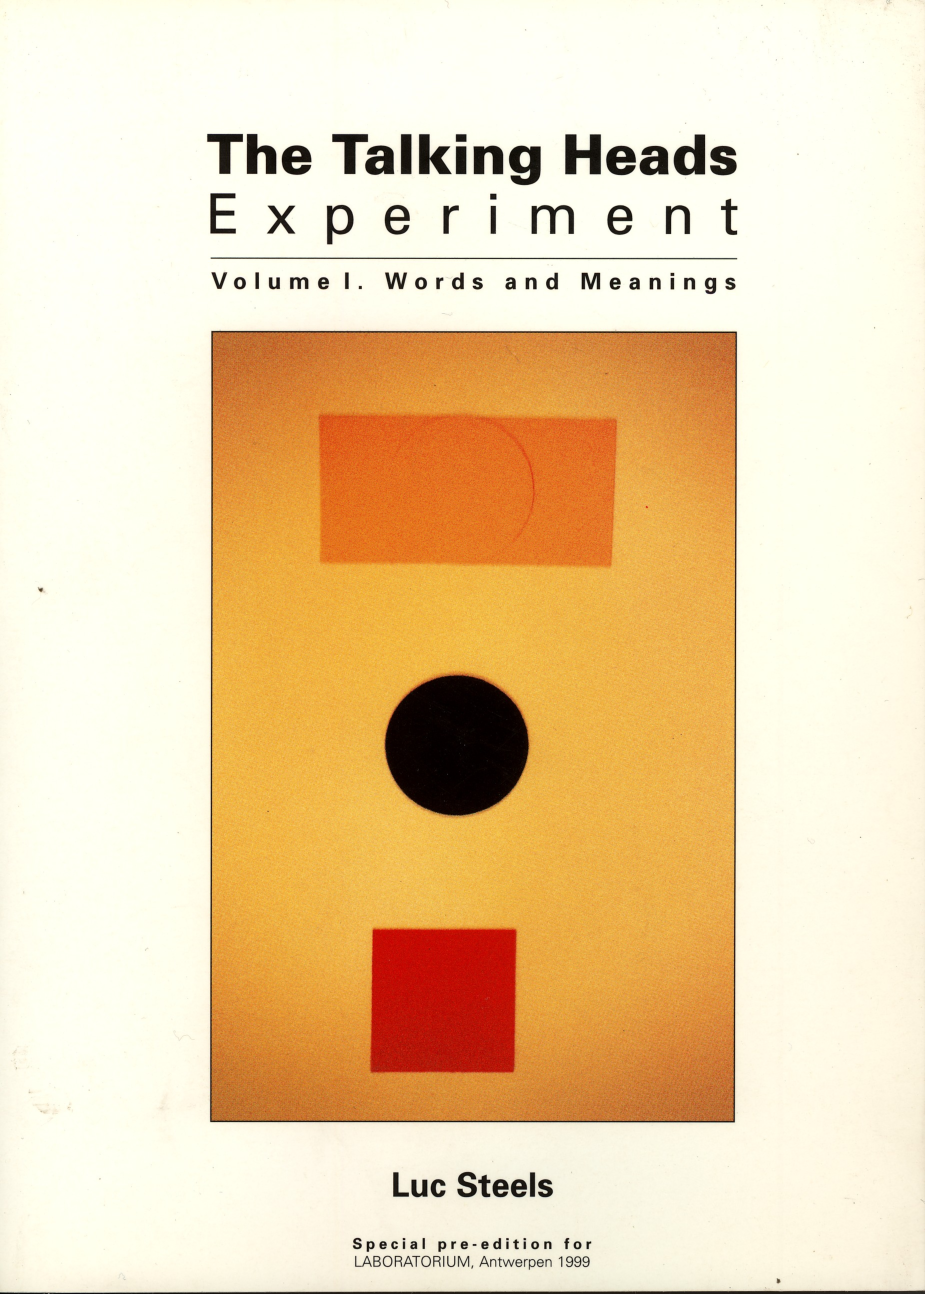
\includegraphics[width=1.0\textwidth]{extra/figs/cover-original-book}}
\caption{\small\label{left-right} Original cover of the Talking Heads book published in 1999 on the occasion of the 
Laboratorium exhibition in Antwerp.}
\label{f:cover}
\end{figure}
\chapter{Introduction}
\label{c:introduction}
\newcounter{foot}
\setcounter{foot}{1}
Inquiring about the origins of a phenomenon, 
as opposed to merely describing its present state, often 
leads to profound new discoveries. Biology provides a 
wealth of examples. 
Darwin asked the question of the origins of species diversity and 
thus discovered evolution by natural selection. Pasteur
wondered about the origins of life and thus
discovered the role of bacteria in 
human diseases. My approach in this book is going to 
be similar. In order to advance our understanding 
of human language and cognition, I propose to address
the fundamental question how language 
and meaning might ever have originated. I will not do 
this by a historical reconstruction, nor by an 
empirical investigation of child language acquisition or 
by examining data from the birth of new
languages.\footnote{
There has been a renewed interest the last five
years in the 
question of the origins of language from these various 
perspectives. \cite{Hurford:1998} contains 
a representative sample of the most recent work. 
Other samples of recent research 
can be found in \cite{Hawkins:1992} and \cite{Velichkovsky:1996}. 
}
Rather, 
I will pose the question in a completely general way: 
how can a physically embodied autonomous agent \is{agent} arrive 
at a repertoire of categories for conceptualising his
world and how can a group of such agents ever develop 
a shared communication system with the same complexity 
as human natural languages. 

\section{The Talking Heads experiment}

For centuries, philosophers, linguists, psychologists and 
neuroscientists have been groping with the amazing capacities
of the mind. By necessity, they have been doing this through
thought experiments or by observing human behavior and
brain anatomy. Although this has generated a wealth
of insights,\footnote{Attempts are made to bring together the insights from various
disciplines to establish a true `cognitive science'. 
\cite{Osherton:1995} contains an introduction into some of the main 
research trends in this very diverse scientific field. 
See also \cite{Luger:1994}. The work reported in the present book can be 
classified as theoretical
cognitive science because I try to formulate and test
the operational adequacy of possible models for the 
origins of language and meaning but do not claim nor
give any evidence that these models are also valid for
human cognition, just as the study of aerodynamics and 
aircraft design may help to understand how birds can 
fly but is more generic than its biological 
implementations.}
everyone involved in this research must surely 
agree that we are still lacking adequate models, 
particularly for higher order cognitive functions like language
processing, and definitely for understanding how such 
functions may have arisen. 
To discover or test such models, it therefore
remains useful to do experiments with artificial systems.
We can build robots that receive sensory inputs
through a camera or other sensors, give them computational 
power and memory, and empower them 
for action in the world by adding actuators. Given such a 
set-up, we can precisely examine the operational adequacy 
of an hypothesis. For example, if someone proposes
a process for segmenting images, we can test this process 
by capturing streams of images through a camera and 
see whether the process is indeed capable of performing 
segmentation. When someone proposes a process 
for parsing sentences, we 
can implement this process and confront it with a series of 
example sentences to measure success and failure. 
How else can we test the operational adequacy of a proposed
cognitive model, given the enormous complexity involved? 
Of course, building an artificial system in no way proves
that the principles that were used to construct it are valid
for natural systems. But it is an enormously valuable 
source of insight for approaching the extraordinarily 
complex phenomena observed in human cognition. 

\begin{figure}[htbp]
  \centerline{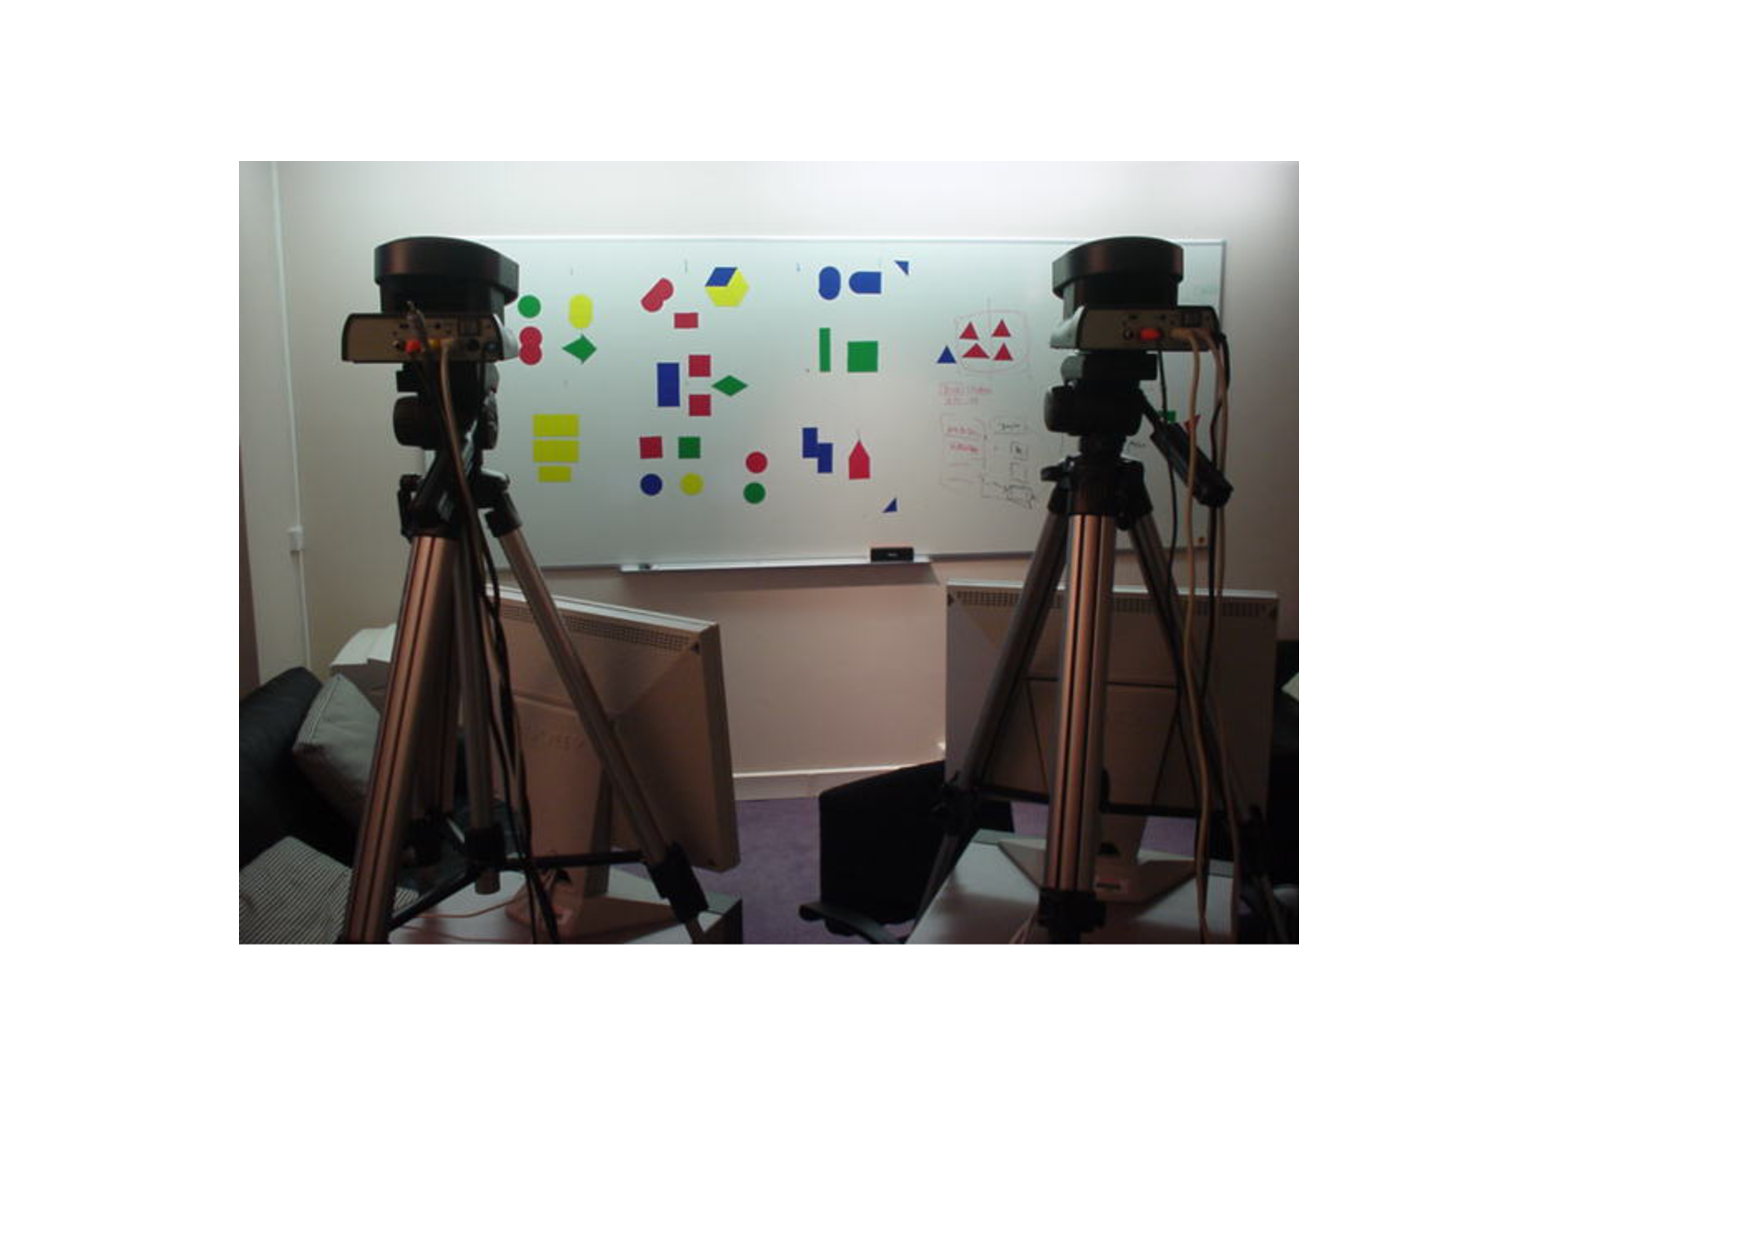
\includegraphics[width=.65\textwidth]{chap1/figs/heads}}
\caption{Two talking heads are shown {\bfshape a1} and 
{\bfshape a2} each seeing the scene on the white board from a slightly different viewpoint.}
\label{f:plate1}
\end{figure}

The Talking Heads experiment follows this research strategy. \is{Talking Heads Experiment}
It features an enormously challenging experimental
infrastructure to explore how a cognitive
system, like the one underlying human language, might
be able to bootstrap itself into interaction 
with other cognitive systems and driven by increasing
challenges from the environment. The experiment
involves a set of robotic `Talking Heads' engaged in language
games, with each other or with human interlocutors, 
about real world scenes they perceive through their sensors
(see Figures \ref{f:plate1} and \ref{f:plate2}). 
The robots use vision as major sensory source. They are located in
different places in the world and connected through the Internet. 
Two robotic agents can only engage in an interaction when they 
are instantiated in robot bodies in a shared physical environment. 
After an exchange, an agent can teleport himself to another body in 
another location and engage in interactions there. 

\begin{figure}[htbp]
  \centerline{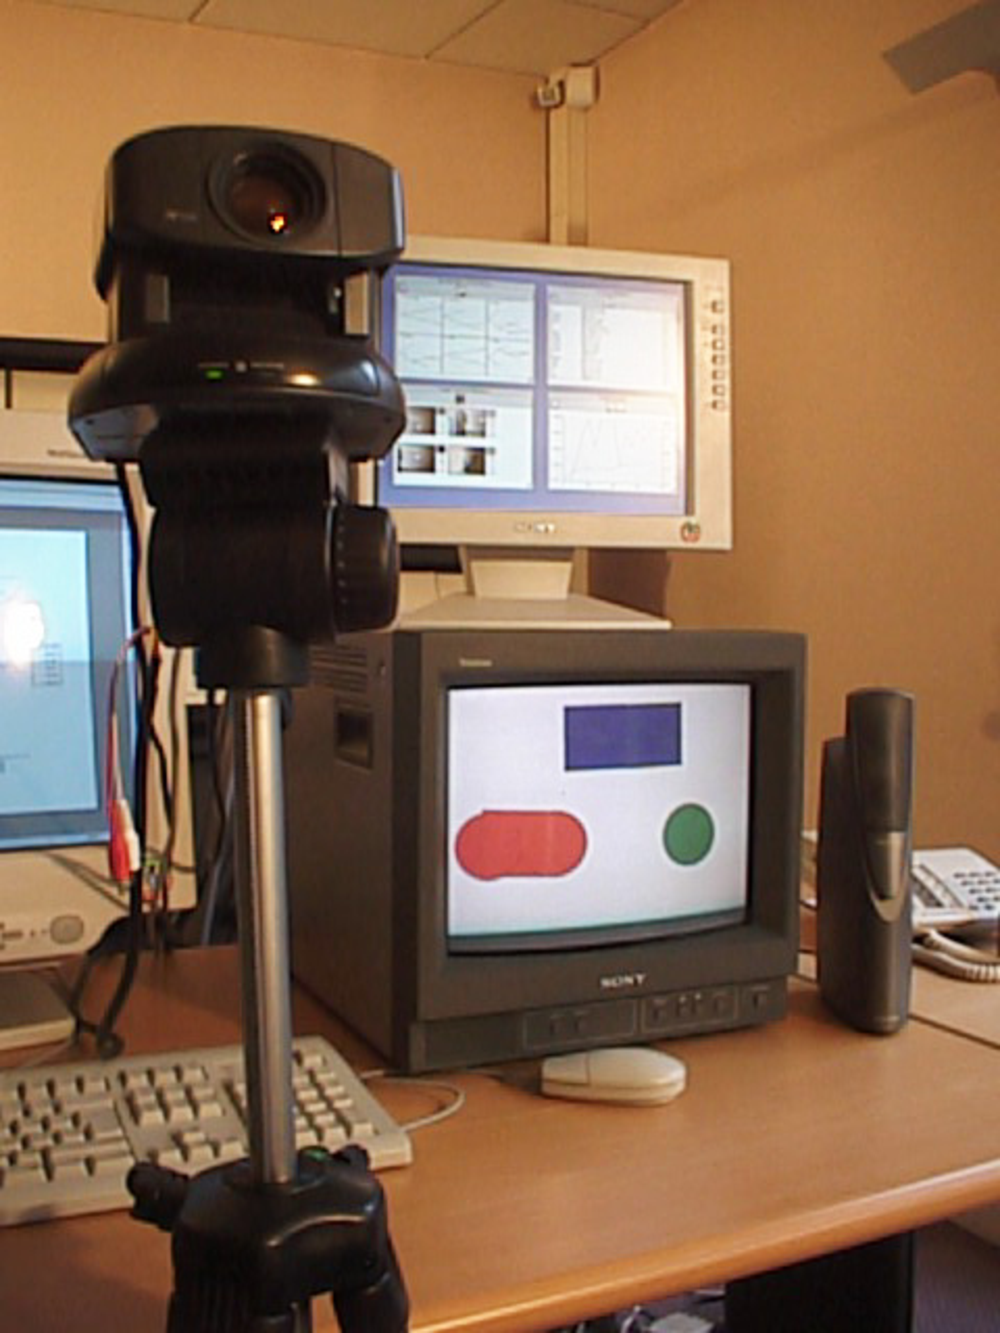
\includegraphics[width=.40\textwidth]{chap1/figs/head}}
\caption{ A single 'talking head'. There is a camera oriented towards a
white board. The bottom screen shows what the camera observes. The top right screen shows the result of processing.
A loudspeaker reproduces the utterances of the agent. }
\label{f:plate2}
\end{figure}

The agents' categorizations of
the world and their language is {\itshape not} programmed but
emerges. It is 
constructed and learned by the agents themselves. The more 
interactions they have with other humans the more they 
adopt our concepts and language. Interacting with the Talking 
Heads is a bit like interacting with two year old 
twins; they play  most of the time with each other and
develop their own language in the process, but the more
humans engage in interaction with them, the more the language
resembles existing human languages.\footnote{Often twins develop a private language, particularly 
if they do not interact much with adults. Compared
to other children, twins are usually 6 months behind 
in their language development but that delay and 
also the private languages that go with it disappear
by the age of 8.}

Although the agents invent their own 
language and conceptualisations of the world, we
had to program a basic cognitive architecture into 
the agents. This architecture is based on a set of relatively
simple, biologically plausible mechanisms, which 
nevertheless gives rise to enormous complexity.
The goal of the experiment is to examine the explanatory power of 
these mechanisms: What phenomena do they cause and
hence explain. 

\section{The main hypotheses}

The Talking Heads experiment is first and foremost
a scientific experiment. It subjects four radical ideas 
to experimental scrutiny. 
The first idea is that 
language emerges through self-organisation out of local
interactions of language users. It spontaneously 
becomes more complex to increase
reliability and optimise transmission across generations of 
users, without a central designer.
I call this {\itshape the selfish
language hypothesis}: Language colonises
brains and recruits available cognitive capacities to satisfy
its appetite for expressing ever more complex meaning with
minimal effort and maximum 
effectiveness.\footnote{
See \cite{Deacon:1998} for a discussion of 
co-evolution between cognitive and linguistic
capacities and brain structures.}
Language is 
not a uniform abstract system of rules (and definitely not an 
innate system of rules) but a creative open-ended complex
adaptive system, like a natural
ecology, in which certain solutions to relate forms with 
meanings become temporarily conventionalised in 
the community, even though new creative solutions
emerge almost any time someone speaks. Language
is in constant flux because new meanings continuously
arise and existing forms undergo change beyond the 
control of any individual language user. 

The second radical idea is that 
meaning is built up slowly by each individual in a cumulative
growth process. Meaning is not innate, as rationalists in the 
footprints of Plato have been arguing for centuries, nor 
learned through stepwise
induction from examples and counterexamples, as empiricists
have been saying. Meaning is at first very concrete and
strongly situated in the environment and bodily experiences.
I will take the suggestions made
by Wittgenstein \is{Wittgenstein} one step further, namely that meaning (and language) is constructed
and practised as part of
language games.\footnote{\cite{Wittgenstein:1953} emphasises the relativity 
of concepts and the role of language and hence
meaning in social interactions.}
I will introduce a selectionist approach to
the acquisition of meaning, introducing models to 
show that conceptual distinctions can `grow' in the brain
like the leaves and branches on a tree and be pruned to fit the
demands and characteristics of the environment in which
an agent finds itself. Even though non-verbal 
activities, like predicting the future based on a model 
or deciding what to do in specific circumstances, stimulates
the growth of distinctions, language use is probably one 
of the greatest stimulators of conceptual growth. It provides
feedback about which distinctions were successful in linguistic
communication and thus whether or not they should be preserved. 
Thus language and cognition co-evolve. Each one pushes the other 
up towards more complexity and they become tightly 
co-ordinated with neither a central co-ordinator nor prior innate design. 

A third idea concerns the characteristics of
cognitive architectures.
For centuries, the human cognitive system has been 
likened to a machine, most recently to the computer as 
an information processing machine.\footnote{See \cite{Newell:1976}}
Although there is a lot to say for adopting such a 
viewpoint, I will instead emphasise biological metaphors. 
Specifically, I will defend the idea that a living ecology 
is a better metaphor for a realistic cognitive system. 
In an ecology, there is constant change as 
the individual organisms adapt themselves to the 
physical environment and to other organisms sharing 
the same environment. There is evolution by selection so 
that successful adaptations survive and others disappear. 
There are failures but also repair processes 
happening at all levels of the ecological 
hierarchy. These various characteristics inspired
the artificial architectures used in 
the experiments. 

A fourth radical idea concerns the nature and origins of 
grammar. Rather than invoking the need of a highly 
specialised genetically determined language 
organ\footnote{
As strongly argued by Chomsky in various writings. 
See for example \cite{Chomsky:1968}. 
Praeger, New York. Even though Chomsky argues for 
an innate language acquisition device he has expressed
scepticism about evolution by natural selection
as an explanation for the 
origin of this device (and therefore of language). 
A genetic theory of language evolution 
has been suggested by \cite{Pinker:1994}.}
I believe that grammar spontaneously arises when 
generic capabilities to categorize reality, store past
events in terms of abstract schemas, remember associations
between events, etc., reach a critical level and are
applied to language itself. These capabilities are 
relevant across many different cognitive domains. 
In order to store linguistic
experiences, human memories spontaneously structure them, thus 
introducing abstract schemas, internal categories, and 
roles that substructures can play in schemas.
These organisational elements then become externalised. 
Categories are marked by enriching
the form of words, schema boundaries are marked by 
imposing patterns on the expression of a schema, 
roles are marked by assigning
them to specific positions in a 
pattern. This externalisation 
increases the reliability in communication because
it reduces ambiguities and supplies additional context. It 
also aids the stable transmission of the language from one
generation to the next because the language learner
gets additional hints to guess the meaning and function of unknown
words and constructions. 
Once such structuring devices are in place, they help 
to increase the expressive power of the language. The 
complexity of possible language interactions can increase, 
and words or word groups which had multiple usages
can become specialised for particular semantic functions. 

The various language construction processes gradually 
shaping a full-blown language 
are not under the conscious control of individuals but
instead constitute a collective enterprise. Language users 
structure and restructure their language and thus increase its
systematicity, but there are also forces causing a breakdown 
of systematicity, such as erosion of a form 
through sloppiness of pronunciation, in turn causing a grammatical 
regularity to break down. The interplay between 
these constructive and destructive forces helps to explain
the constant evolution of language and the growing 
diversity among languages emanating from the same source, such as
French, Italian, and Spanish from Latin. 

\section{A bottom-up approach to artificial intelligence}

\is{bottom-up approach} My daughter Lenie grew up surrounded by computers and 
robots which her obsessed father was trying to infuse
with artificial intelligence. When she was twelve, I asked
her whether she thought any of the machines or 
programs she had seen were intelligent. 
She said no, someone had programmed them, so they were
not intelligent themselves. The programmer was 
intelligent, not the machine. Indeed, this is true. 

In 1996, a computer program called Deep Blue
defeated the reigning world champion Kasparov in a game of 
chess.\footnote{See: \cite{Newborn:1996}}
Kasparov was astonished
and depressed, and claimed this was a defeat of humans in 
the 
race against machines. But was he actually beaten by {\itshape artificial}
intelligence? Not really. A team of engineers and scientists
from Carnegie Mellon University and from the IBM Watson 
research center had been working for ten years to program 
vast amounts of chess knowledge, invented by
human experts, into Deep Blue. They had built extremely 
sophisticated dedicated computing hardware to
apply this knowledge at a blinding speed. So, in beating Kasparov, 
other humans were the clever ones, not machines. 

Recently, the whole world looked on in fascination
for several weeks as a small robot, the Rover Sojourner, ventured
out on Mars, navigating through the rocky landscape, collecting
samples, taking pictures and performing 
experiments.\footnote{
See \cite{Wunsch:1998} (a book for children!)}
Was this a first sign of artificial life?\is{artificial life} Even though the 
behavior of the robot has some apparent characteristics
of living systems, people more
familiar with the project would say no. 
The robot was hardly autonomous; it continuously had to rely
on signals coming from human engineers in order to set
its next targets, or to deal with unforeseen circumstances. 
The robot's behaviors were
all human designed and carefully programmed. The robot 
itself was in no way adaptive. It did not learn new behaviors
nor new interaction modes, as a living system would do.
It was critically dependent on human engineers whenever its
functionality needed to be extended or modified. 

This in no way diminishes the achievement in
building these artificial devices, on the contrary, it
does show we have to be careful in ascribing mental or biological
qualities to machines. Despite the hype generated by the
media and the occasional researcher taking his dreams for reality, 
intelligence and life remain very much the property of
natural rather than artificial systems. In a way, our
powerful engineering methodologies make it too easy to 
succumb to a strategy of programming directly the human or animal 
behaviors we observe and interpret as being 
intelligent. But doing this, we keep simulating 
the end products of intelligence rather than getting at the heart of 
intelligence itself. We put our own human concepts explicitly
in the machine instead of implementing the mechanisms that
enable an artificial agent to acquire new categories itself, 
implementing by hand a fixed set of predetermined behaviors which 
we believe the agent should have, 
rather than supplying mechanisms that allow the agent to acquire new 
behaviors when faced with unforeseen circumstances, 
and so on. Things are done this way because we simply 
do not know how to do them otherwise. 

The goal of the fundamental research
reported in this book is not only to raise some 
profound fascinating questions about language, but also to lay 
the groundwork for an alternative bottom-up approach towards
artificial intelligence. In this approach, the human 
designer does not put his or her language and 
concepts into the computer, but tries to set up systems that
autonomously generate their own. Indeed, if we have scientific
models which explain how language originates, both in a language
community and in new individuals born 
into a community, we should be able to operationalise 
these models and show that they work on autonomous robotic
agents. This is exactly what the Talking Heads experiment
tries to accomplish. 

\section{History of the project}

The Talking Heads experiment is the culmination of one of
the most exciting scientific and engineering projects I have
ever been involved in. It has required the
creative efforts of a dozen excellent researchers 
over many years. The story started in 
1985. Instead of continuing to design and program intelligence
explicitly based on formalising human cognitive
capacities, as most of my colleagues
in artificial intelligence research 
labs were doing,\footnote{
Some recent overviews of this `classical' approach to 
artificial intelligence can be found in: \cite{Nilsson:1998} and 
\cite{Russell:1998}}
I started to focus on the 
question of how intelligence might
originate and evolve in physical agents as they 
interact autonomously with their environment or with 
other humans, and I encouraged my students
at the Artificial Intelligence laboratory of the University 
of Brussels (VUB) to experiment in the same direction. 
We initially developed a bottom-up, 
behavior-oriented approach to sensori-motor intelligence, 
which was also being explored around the same time by 
Rodney Brooks at the MIT Artificial Intelligence 
laboratory.
The behavior-oriented, bottom-up approach \is{behavior-based robots} was a 
counter reaction to the symbolic, top-down approach of 
earlier AI research. See \cite{Steels:1995} and \cite{Arkin:1998}. 
We built robots of various sizes and shapes, using simple
electronic circuits, Lego bricks, small motors, rechargeable
batteries, self-made 
sensors, single board computers, and everything else that 
appeared useful (\figref{f:plate3}). 

\begin{figure}[htbp]
  \centerline{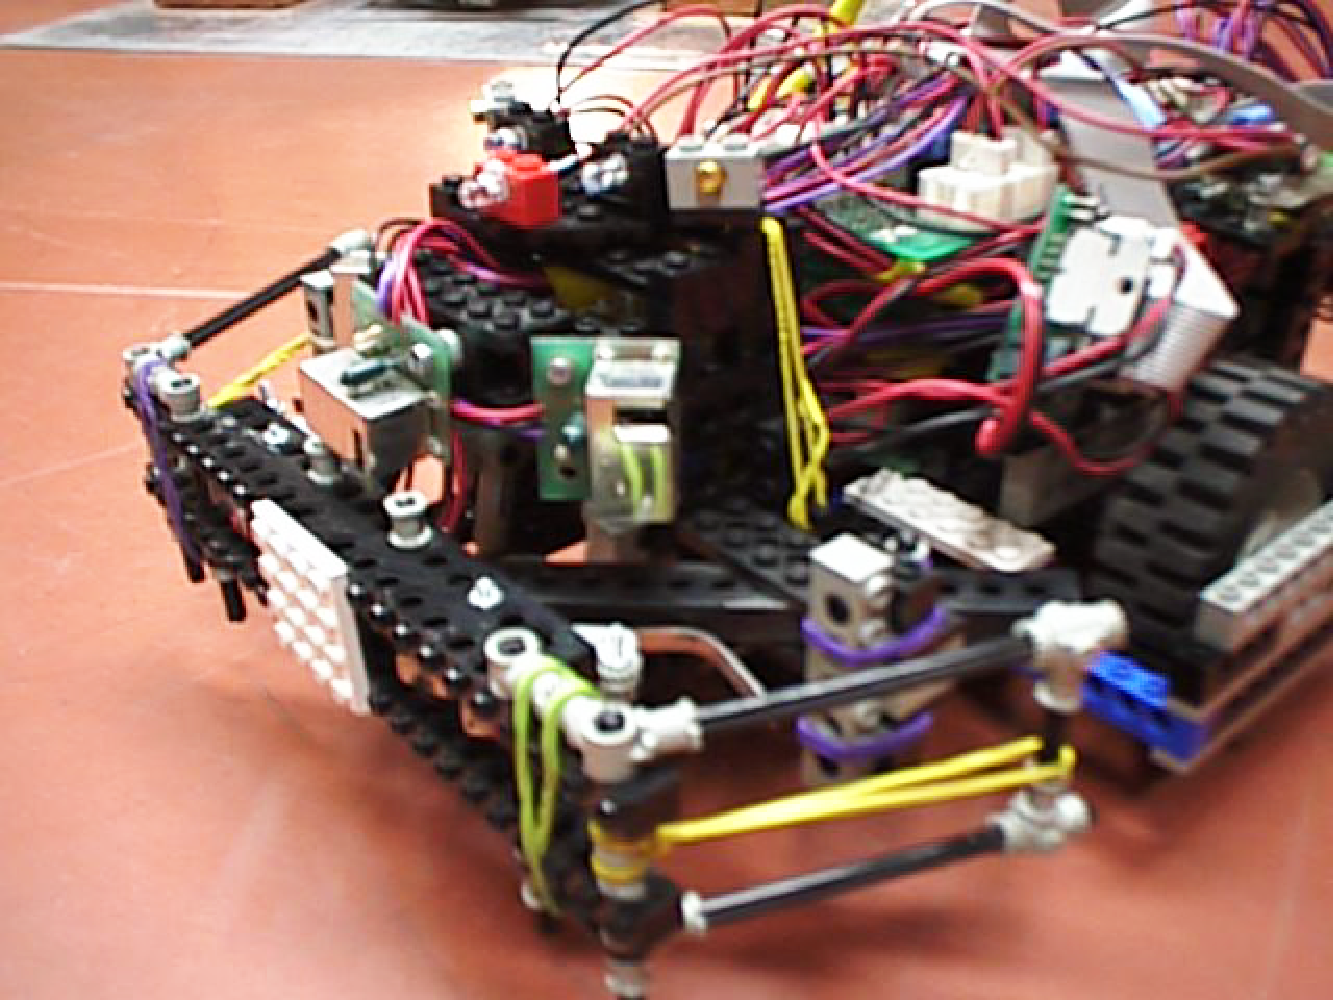
\includegraphics[width=.60\textwidth]{chap1/figs/robot}}
\caption{ Example of a 'Lego vehicle' built by Tim Smithers based on Lego bricks, a sensori-motor processing board, 
and a variety of 
sensors and actuators. We developed these robots in the early nineties for exploring a behavior-oriented 
approach to robotics.}
\label{f:plate3}
\end{figure}

Most robots drove around on wheels, but we also used balloons and propellers to build 
flying robots and experimented with a fish-shaped robot which swam in the university swimming pool by wagging 
its tail (see \figref{f:plate4}). 

\begin{figure}[htbp]
  \centerline{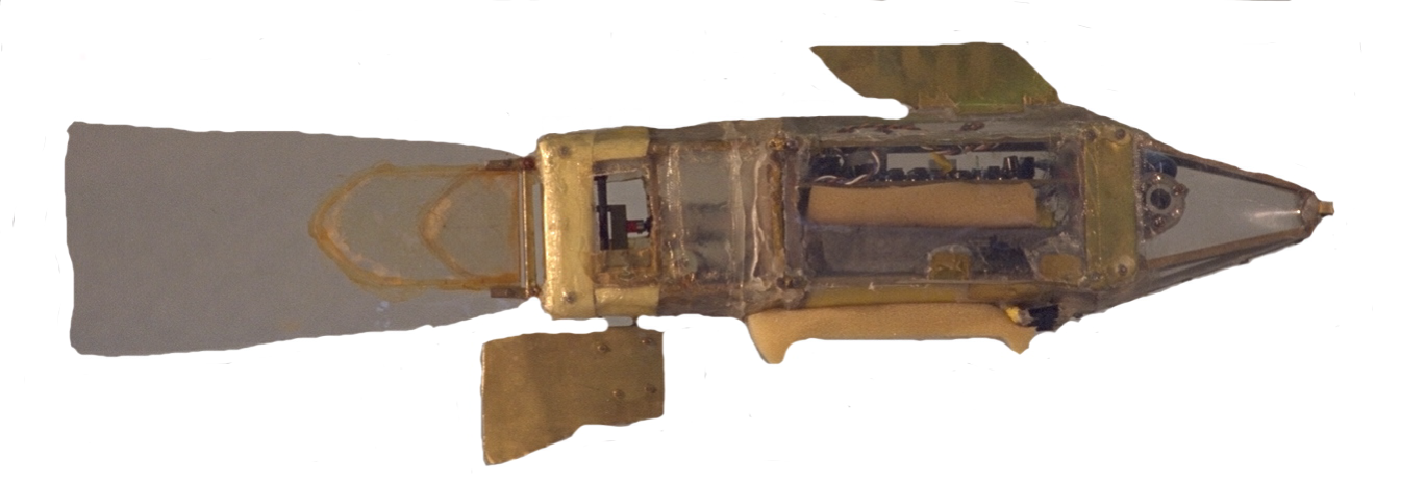
\includegraphics[width=.85\textwidth]{chap1/figs/fish}}
\caption{ Artificial fish built by Miles Pebody to explore influence of robot bodies on behavior. The fish could swim around by wagging 
its tail and avoid obstacles based on infrared sensing.}
\label{f:plate4}
\end{figure}

To investigate the role of the environment in shaping the
evolving sensori-motor capacities of these robots, 
we built various robotic 
ecosystems in which robots could recharge themselves but also
had to work for their living by 
dimming lights that took away energy from the total energy 
flowing in their ecosystem  \ref{f:plate6}). Visitors
to our lab could see robots helping each other or 
engaging in fierce competition for
the resources available for survival. In all of this
research, we tried to see how far behaviors would
autonomously evolve, in other words we tried to find 
mechanisms by which the robots would bootstrap themselves 
towards greater sensori-motor complexity. One of the 
main lessons from these experiments was that 
explanations for cognition lie partly outside the brain 
of the individual agent: The environment, the body, the 
sensori-motor apparatus and the behavior of the other 
agents all partly shaped their capacities and 
further development.\footnote{This approach is also known as `situated cognition'. 
\cite{Clancey:1997}, see also: \cite{Varela:1991}.}

\begin{figure}[htbp]
  \centerline{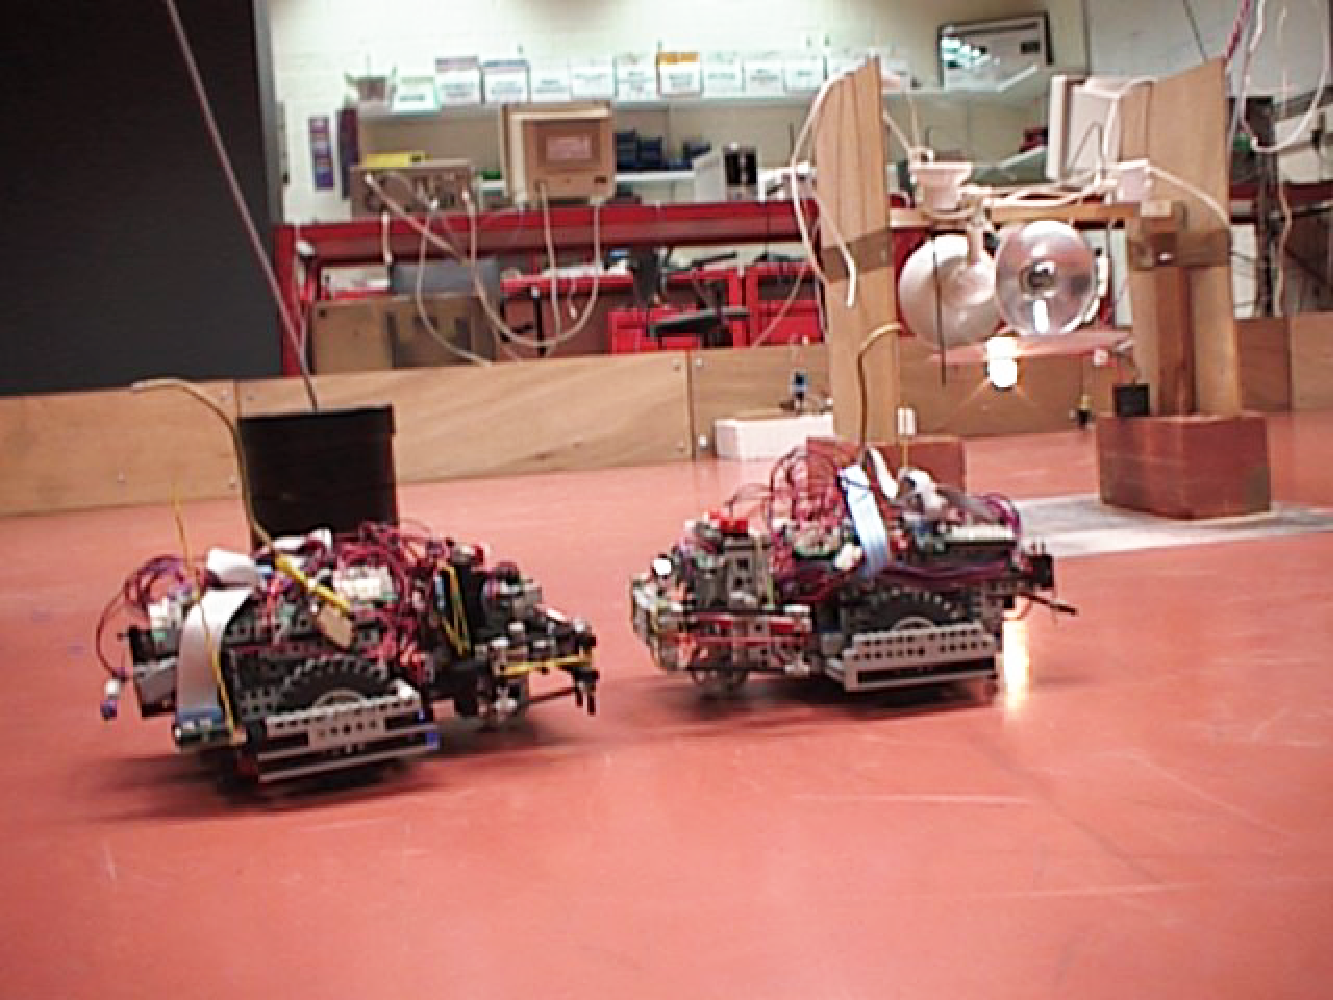
\includegraphics[width=.80\textwidth]{chap1/figs/ecosystem}}
\caption{ This ecosystem was designed together with David McFarland (Oxford University) to explore 
emergent cooperation and competition. The robots in the form of lego vehicles could recharge themselves in the charging 
station (shown in the right top corner). But they had to ensure that there was enough energy in the charging 
station by dimming a light in black cylinders by pushing against them.}
\label{f:plate6}
\end{figure}

Many fascinating tales can be told about this research but the intelligence being exhibited 
by these autonomous robots hardly seemed worthy of the name. Yes, they learned
by themselves how to avoid obstacles, how to recharge themselves
in a charging station, or how to co-ordinate efforts 
to exploit the resources in the ecosystems we had built for 
them. But critical observers did not see much more than 
rat intelligence and they were right. The original 
goal of reaching human 
cognitive levels, as observable for instance in 
expert problem solving or conversations in natural
language, remained elusive. The 
traditional Artificial Intelligence
approach of explicitly programming symbolic intelligence
still gave far superior performance in tasks requiring
cognition. Clearly, essential theoretical concepts were 
missing for a truly bottom-up approach to succeed. 

In the summer of 1995, a clear breakthrough occurred.  
I was working as a visiting researcher in the Sony
Computer Science laboratory in Tokyo, invited by its director
Mario Tokoro. Reflecting on our 
experiments from a distance, two new ideas occurred to me. 
First of all, language may have been the missing key
in the initial experiments. Language may 
be a necessary route by which the human cognitive system
bootstraps itself autonomously, in tight interaction with the
environment and aided by a community of other
language speakers. This suggested that if we wanted
to have emergent
forms of cognitive intelligence, we needed to go the same 
route. Second, the principles and mechanisms that had been
pouring out of the study of complexity had to be
relevant to understanding the origins and evolution of language,
because they provided generic explanations for how complexity 
may emerge. These principles include 
self-organisation, structural coupling, 
selectionism, level formation, 
and many others, \cite{Nicolis:1989}. The field of `Artificial Life' brings together researchers
exploring the insights of complex systems with computational
and robotic experiments, \cite{Langton:1995}.

Together with 
other researchers interested in the then-arising field of `artificial life', I had 
already been simulating path formation in 
ant societies and other biological phenomena exhibiting 
an emergence of complexity. It dawned on me that the
importance of these mechanisms for bootstrapping intelligence and
language might be much greater than 
thought so far.\footnote{The following reference provides a general survey of similar work in 
the area of lexicon formation: \cite{Steels:97b}. 
A representative sample of more recent work on syntax, is \cite{Briscoe:1999}.}

Back in Brussels, an extremely exciting but very 
intense period of research started as I tried to 
apply these principles to language
and subject them to experimental 
scrutiny.\footnote{The earliest papers on these mechanisms are in: \cite{Steels:95b} and 
\cite{Steels:96a}.}
We very quickly built a first 
prototype of a `Talking Head' with our own hardware
and low-level software (see \figref{f:plate7}) 
and experimented with language games on mobile 
robotic agents.\footnote{The electronics and tracking software for this 
active camera were built by Tony Belpaeme. The mobile
robot experiments were conducted with Paul Vogt \cite{Steels:97g}. 
Other early work on the grounding and autonomous acquisition of 
language-like communication systems by robotic systems is 
described in. See also: \cite{Billard:1998}.}
New fundamental insights and discoveries emerged almost daily. 
The first experiments, particularly in grounding
language on real robots, were extremely difficult but we 
were clearly making steady progress. 

\begin{figure}[htbp]
  \centerline{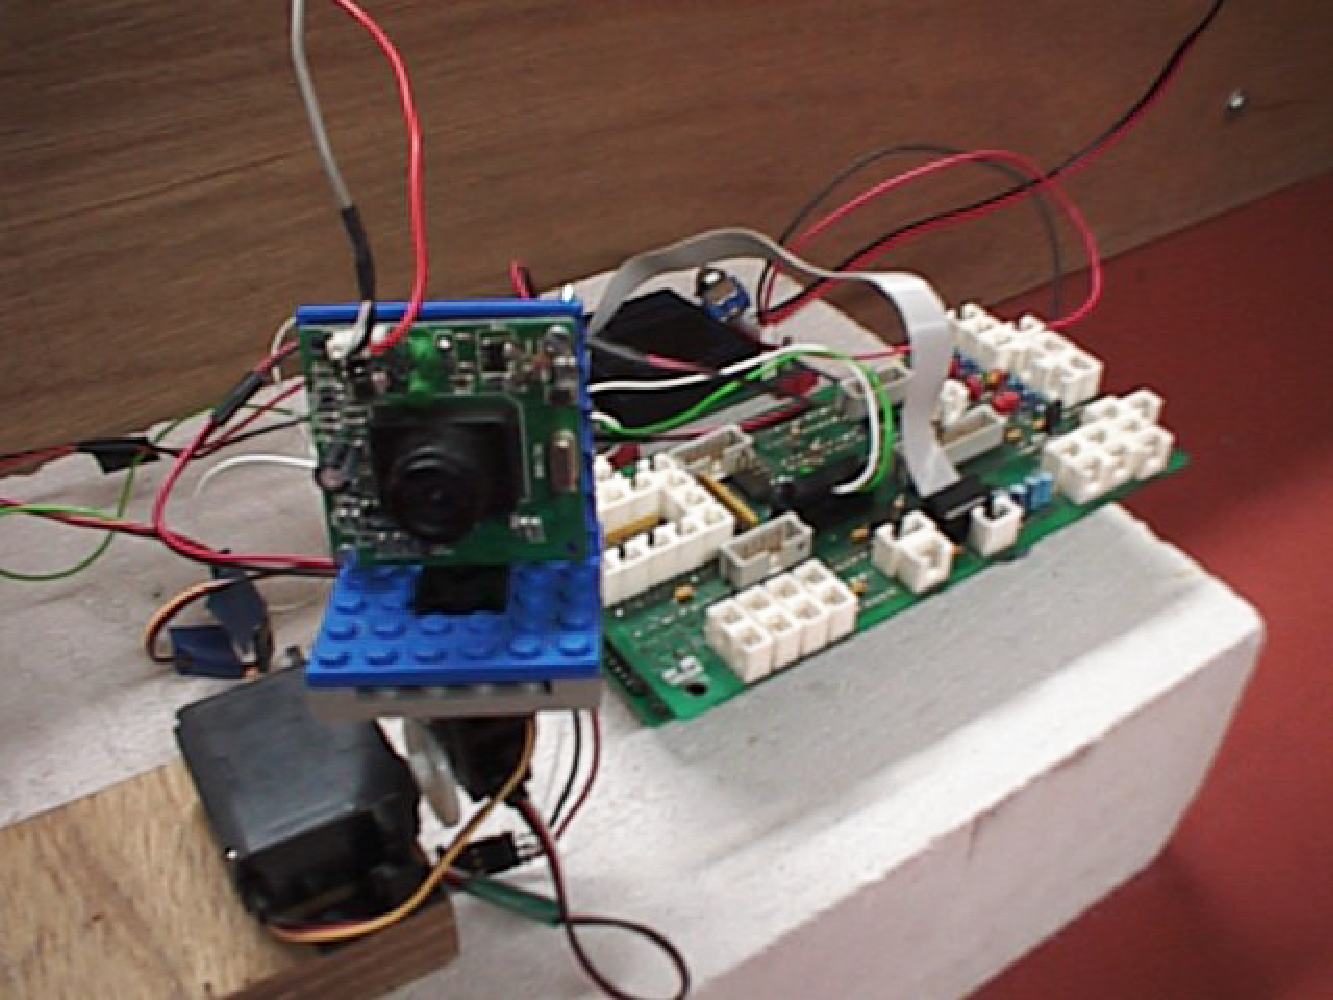
\includegraphics[width=.70\textwidth]{chap1/figs/eye}}
\caption{ First prototype of a `Talking Head' camera with 
associated electronics built by Tony Belpaeme. The camera is capable to track moving images. }
\label{f:plate7}
\end{figure}

As my research program grew more radical, it became more 
and more difficult to get funding. 
European `research' and development programs were 
increasingly demanding short-term projects that targeted information
technology products already available on the American or Japanese 
market. Increasingly, my
research proposals were being rejected and running projects were
cut off,
as reviewers could not see direct short-term 
commercial benefits. All this was endangering the further existence
of my Brussels laboratory, whereas I, paradoxically, thought that
our research had never been more promising. 
Fortunately at this critical moment Mario Tokoro
helped me again in a crucial way. He understood what I was
hoping to achieve and ensured secure and stable resources from 
the Sony Corporation. At the end of 1996, I consequently set up a new research
structure in Paris, a spin-off from the Sony Computer Science
Laboratory in Tokyo, where the bulk of the research reported
in this book could be done in almost ideal circumstances. 
The Paris research was complemented with many important 
contributions of my graduate students
at the VUB AI laboratory in Brussels. 

\section{Beyond Turing}

A scientific experiment creates, in a controlled
and repeatable way, phenomena which shed light on
similar phenomena observed in the natural
world. Initially there is
always some discussion about the relation between 
the artificially created phenomena and the natural
phenomena. Galileo dropped cannon balls from
the tower of Pisa and claimed that these experiments validated 
a general theory of falling bodies; but his contemporaries 
objected that birds graceously landing on a roof can
also be seen as falling bodies, so how general was 
his theory really?  

When dealing with cognitive phenomena such as language
and meaning, the same problem arises. To what extent
do the languages constructed by the Talking Heads count
as languages? Does it make any sense to say that these robotic 
agents categorize their world? Do the Talking
Heads learn? Do they genuinely understand each other? Do they 
understand us? To what extent 
is there a real increase in syntactic 
complexity? Intense discussions about whether cognitive phenomena can 
be recreated in artificial systems 
have raged since researchers have been exploring this 
route, and they have been shown extremely difficult to resolve to 
everyone's satisfaction. 

It seems unavoidable that there is disagreement because 
judgements about cognitive capabilities are to some 
extent subjective. Most people ascribe more intelligence
to their pets than a casual observer is willing to admit. 
In any case, judgements should clearly rest with humans, and
definitely {\itshape not} with the designers 
who are all too keen to call their systems intelligent. 
This was clearly recognised by Turing \is{Turing test} when he devised
his famous Turing test.\footnote{The Turing test is originally described in 
\cite{Turing:1950}.} Turing started from a popular societal 
game of his time, where an observer had to tell through
a dialog whether he was talking to a man or a woman. 
He proposed to call a computer program intelligent when 
it was capable of playing the role of a man or woman
so well that the observer could no longer tell whether
a person or a computer program was playing the game. 
The Turing test has rightfully been criticised as being
on the one hand too difficult, because it is completely 
open-ended, and on the other hand too narrow, because it 
does not incorporate important aspects of intelligence such 
as learning or sensori-motor intelligence. The only way 
to have a decent showing in the Turing test is to
cheat, i.\,e. to let the computer mimic intelligence 
by manipulating symbolic patterns without any notion of what 
they mean. It is therefore desirable to have an alternative
set up which still preserves some of Turing's original 
ideas. 

The goal of the Talking Heads experiment is not to demonstrate 
an artificial intelligence with the same capacities as 
human intelligence, but to perform
scientific experiments so as to examinine aspects 
of a theory of the origins of language and meaning. 
However, as in Turing's proposal, the public should be 
the ultimate judge whether cognitive phenomena are taking
place, and the artificial agents should be able to play their role
in interaction with humans. 
Sound scientific methodology requires that 
the experimental apparatus is a white box which can be fully probed 
by anyone who wants, that the experiments are repeatable, 
and that the phenomena that are generated 
(for example, the complexity of the lexicons or 
grammars) can be 
compared by anyone to human cognitive phenomena in order to gage 
their similarity and thus their relevance for understanding
human cognition. 

In 1999, a golden opportunity presented itself to 
expose our theories and systems to public scrutiny and thus solicit
judgements from a wide range of human observers. Barbara
Vanderlinden and Hans-Ulrich Obrist, two internationally 
renowned young curators, had been put in charge of 
an important art event in the city of Antwerp (Belgium)
and made the brilliant decision to organise a 
confrontation/co-operation between art and 
science.\footnote{The catalog of this event, edited by Obrist and Vanderlinden \cite{Obrist:1999}, gives an idea of 
the other laboratories and the coming together of art and science.}
They invited \is{Laboratorium exhibition}
artists and scientists to set up 
a public laboratory in the city and conduct experiments 
from the viewpoint of their discipline. This is how 
the Talking Heads experiment came to be installed in 
a public space in Antwerp and how thousands of people, 
some more bewildered than others, took part in the first
ever large-scale public experiment in artificial intelligence. 
Everybody was encouraged to interact with the robots and 
to try and understand what was going on. This was not an obvious
thing to do because the Talking Heads
construct their own language and their own conceptualisation of 
the world. Understanding what they are talking about, resembles the work 
of an anthropologist who is studying the language and
conceptualisations of a newly discovered tribe living
secluded in the rainforest. 

The `laboratory for cognitive robots and 
teleportation' that housed the 
Talking Heads experiment also contained  
a documentation room in which the audience could 
get additional background information and 
provide feedback and commentary 
on the experiment. We created a Web site that was accessible 
worldwide through the Internet. This allowed viewers from anywhere
in the world to follow the dialogs, inspect the lexicons
and ontologies 
of the robots, and even interact remotely with the 
physical robots, playing language games 
and doing their own experiments. We also added
other physical sites in Tokyo, Brussels, Paris, Amsterdam, 
San Jose (US) and other places, to increase the environmental complexity that 
the agents could experience. 

The massive response and thoughtful judgements of the 
public were crucial to validate many aspects of the 
theories put forward in this book. 
But the interactions with a broad public and
the intense discussions that it generated also added new
dimensions to the research. First of all, a whole 
new type of interface between man and machine was
taking shape under our very eyes. In contrast to pre-programmed
computer interfaces, which more often than not make it
difficult to do what one wants, the Talking Heads demonstrated
for the first time the concept of {\itshape negotiated user
interfaces}. The interaction was based on mutual respect
and adaptation of man {\itshape and} machine. Communicative
failure was not fatal but 
an opportunity to fine-tune and negotiate the way communication
would take place in the future. 

Secondly, the Talking Heads experiment turned out to be 
an ideal learning environment for raising philosophical
issues. Children and adults alike
started to ask questions about the nature of
meaning, the relation between language
and reality, the mind-body problem, 
the origins and evolution of language, 
consciousness, social identity, and so on. They 
start to play language games among themselves and some of
them reported profound changes in the way they 
think about language. If these reflections create 
greater tolerance towards other languages and 
the conceptualisations of the world
they implicitly embody, then I consider the
Talking Heads experiment of great societal value, irrespective of
the scientific and engineering breakthroughs
the project has generated. 

\section{The book}

This book describes in detail the rationale behind the 
Talking Heads experiment, the mechanisms that make it
all work, the ontologies (sets of perceptually 
grounded concepts) and 
languages the agents develop, and what happened
when the Talking Heads were exposed to public scrutiny. 
It studies processes which must already be active in the 
very first stages of language use in the child, and 
must also have been present in the early phases of 
human language genesis. 

The main text contains the
principled line of the argument in a form which is intended to be generally
accessible - without compromising exactness. The notes after
each chapter contain references to other work, as well 
as details or additional material of relevance to the 
specialist. Each chapter also contains a set of references to
literature on the same topic. 

This book starts with a preview of the 
experiment and a brief illustration of the core ideas (chapter 2). 
I then cover the 
different tasks step-by-step that speakers and hearers must carry out: 
perception (chapter 3), conceptualisation (chapter 4), 
and lexicalisation (chapter 5). Each 
chapter discusses the 
architectural components with which the Talking Heads 
have been endowed and the kinds of cognitive structures that 
the agents generate in interaction with the environment 
and the other agents. Chapter 6 and 7 then bring all these 
results together and tests the rich complex semiotic dynamics that 
arises when the Talking Heads effectively interact 
with real world environments. 

The research discussed in this book is far from finished. It is 
still science in the making. Many cognitive structures
and capabilities, even very elementary ones arising 
during the first years of human life, are still unveiled. Many
language issues
have not been covered yet. The current set-up 
shows only inklings of what future forms of man-machine
interaction might be like. Nevertheless, I believe that 
the hypotheses proposed in this book, and the 
methodology of experimentation that has been used to 
explore these hypotheses, open new venues for 
a scientific understanding of the human mind. Building 
artificial systems that exhibit cognitive capabilities
does not de-humanise the mind - in the 
same way as the telescope does not demystify the cosmos. 
We see much more and what we see is infinitely more 
beautiful and impressive. 

%\end{document}

%\documentclass{../_combined/fcg-book}
\chapter{Preview}

\setcounter{foot}{1}
When people see the Talking Heads for the first time, they 
are stunned. It takes a while before
one gets used to the self-generated movements of each robot, 
the strange dialogs in an incomprehensible language, 
the graphs plotting the evolution of their internal
states, 
and the colourful environment which is the subject of their 
language games. But after some time, almost everyone gets involved 
in the game and attempts to figure out the language the robots
have developed or to teach them his own. 
Some people come back
day after day to follow the progression
of the language and conceptualisations that the Talking Heads 
build in collaboration with interacting observers.
Children are the first ones to 
start playing with neither fear nor preconception. 

This chapter explains the general setup of the 
experiment and gives a rough idea of what is going on. 
The various principles and mechanisms at work 
will be discussed in more detail later and I will also give many 
more examples taken from concrete interactions.

\section{The Main Components}

Clearly in the development of language and meaning, 
the group and the environment matter. A child 
who grows up without a caring 
community or without sufficient environmental stimuli
never develops the rich cognitive capacities 
normal adults have. From attempts to educate `wolf children'
who grow up in isolation from a human community, or 
impaired children for whom the intensity of early 
interactions are limited, we know that 
there are critical periods
where a community and a challenging environment must be
present otherwise the child's capacities for language
are damaged for the 
rest of his or her life.\footnote{See \cite{Tager:1994}.}

But how can we sufficiently 
recreate these social conditions in experiments 
with artificial systems? 
Building colonies of physical autonomous robots
roaming the world in search of stimulating 
environments and rich interactions with
other robots is not feasable today. So how 
can we ever test seriously situated and 
socially embedded approaches to cognition? 

\subsection{Teleporting}

Let me make a distinction between the physical aspects of 
a cognitive agent and the mental aspects. The physical aspects include the 
agent's body, the sensors and articulators, 
the physical location, the objects in this location, and the other
agents physically present in the environment. The 
mental aspects include the agent's repertoire of behaviors, 
the brain structures and processes
performing categorizations of reality, his
memory, lexicon, grammar, and so on. 
In the case of humans, these two aspects are intimately 
connected and indivisible. We cannot teleport our mental 
faculties into another body, or into another copy of 
our body, even though there have been speculations that 
we could in the future record human 
brain states,\footnote{
Such visions of the future have been put forward
by Hans Moravec \cite{Moravec:1995}. Neither current artificial intelligence technology nor
the state of the art in brain state recording are anywhere 
near to realising these visions.}
I believe that this will still not enable teleportation
because in human brains there is no distinction between 
hardware and software. The architecture of a human brain, 
the physical connections between cells, and the 
biochemical processes in each cell determine the brain's behavior.
There is no separation between a `brain program' and
an interpreter that reads brain programs and 
executes them. The brain is a special-purpose 
hardware device which is unique to each individual. 
To copy such a device we would have to rebuild it physically,
atom by atom, and integrate it in an exact copy of the 
same body. 


\begin{figure}[htbp]
  \centerline{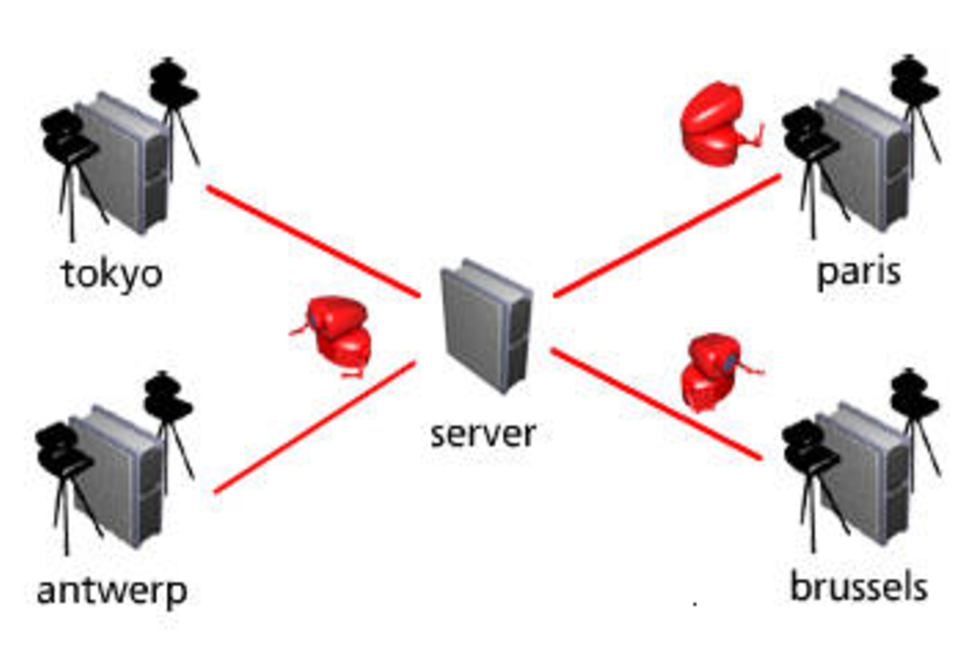
\includegraphics[width=.50\textwidth]{chap1/figs/teleportation}}
\caption{ The Talking Heads agents are implemented as software entities that can travel over the internet. 
To play a game, they get downloaded in a local server that drives the cameras and orchestrates a game. After a game, the software 
state is uploaded again to travel towards another location.}
\label{f:teleport}
\end{figure}

However, in the case of computer-based \is{teleportation}
artificial agents, we {\itshape can} 
make the distinction. It is possible to capture the mental state
of an agent in software, load this into a physical 
body, and then operate 
the agent. Afterwards the agent can extract himself
again from the body, teleport himself 
to another physical location through a data transmission network
like the Internet, get instantiated there in another
body, and experience another reality and physically meet
other agents. This is exactly how we have implemented the 
Talking Heads experiment.\footnote{
The agent teleportation infrastructure is in itself a 
fascinating non-trivial engineering project. Contributions 
from Angus McIntyre, Alexis Agahi, Sylvere Tajan and
Frederic Kaplan are gratefully acknowledged \cite{McIntyre:1999}. 
The fact that agents can teleport proves that we are dealing 
with a truly distributed multi-agent system. It also 
introduces physical parallelism in the agent-agent and 
agent-environment interactions. 
For a general introduction into multi-agent system
technologies and design methodologies, 
see \cite{Ferber:1999}.}
There are on the one hand
the physical structures, which I will refer to as the {\it
robot bodies}. They are installed in different physical 
locations somewhere in the world and connected
with each other through the Internet. Then there is 
a population of software structures that 
are occasionally loaded and instantiated in specific
robots. I will call these software structures
{\itshape virtual agents}. 
A {\itshape real agent} (a Talking Head) 
only exists when the virtual agent is
loaded in a physical robot body. 

Virtual agents cannot interact and 
an interaction between two `real' agents
can only take place when they are both physically present
in the same location. Thus an agent can travel from
Paris to Tokyo at the blink of an eye, rather than having
to take a plane, but two agents can only interact when they
are instantiated in the same physical environment. 
It is in principle possible that agents in different 
physical locations describe to each other the environment that they 
see (but which the other one does not see), just as we 
would do in a telephone conversation. This is only possible,
however, after the agents have had sufficient interactions
with each other in a shared physical world to have 
developed and learned a grounded shared language. 

The teleporting setup enables some fascinating 
experiments, engulfing the 
whole globe. The same agent can look at a scene from
different points of view or at scenes in different
physical locations in the world by teleporting himself in different 
bodies. He can develop categories in one location
and enrich his learning experience by moving to a new 
location which has different objects and thus poses new 
categorial challenges.
There can be populations of varying sizes with new 
agents being born and older agents dying, just like in 
natural human populations, so that we can study the 
transmission of language from one generation to the next
or the resilience of a language against an influx and 
outflux of agents. We can also let agents develop in
different parts of the world and have them migrate to
study intercultural exchange and language contact. 

\subsection{The robots}

A blind person who receives sight after the critical 
period for acquiring visual categorization undergoes a 
traumatic experience, \cite{Zeki:1993}. 
We could in principle build robot bodies
through which agents can experience their world with tactile
sensing and other robot bodies which support visual sensing, or both. 
But then an agent which had only access to tactile
sensing might suddenly find himself in a body equiped with 
vision. This pathological complication will 
be avoided by using the same robotic infrastructure
in every location, even though it would be fascinating and 
technically possible to study multi-modality in its 
own right. 
We also decided to make the robots vision-based, because visual 
sensing is one of the major sources of meaning in
human natural languages. 

Concretely, each robot consists of five building blocks (see \figref{f:plate2}):
\begin{itemize}
\item A camera mounted on pan/tilt motors so that it can move 
up or down and left or right. 
\item A loudspeaker (for voice output) and a microphone (for 
voice input). Each agent has a particular quality of voice
output with male and female voices, so that it is possible 
to keep them apart in the dialog. 
\item A computer that can house an agent's 
cognitive architecture as well as peripheral 
control software to steer the movements of the camera, 
receive and preprocess images, or synthesise and analyse 
sound. This computer is connected 
to the Internet to allow virtual agents to be loaded and instantiated. 
\item A television screen that shows {\itshape us} what the agent
instantiated in a body currently sees through the camera. 
\item A computer screen that shows {\itshape us} what is going on inside
the brain of the agent currently installed in the robot (\figref{f:agentview})
\end{itemize}


\begin{figure}[htbp]
  \centerline{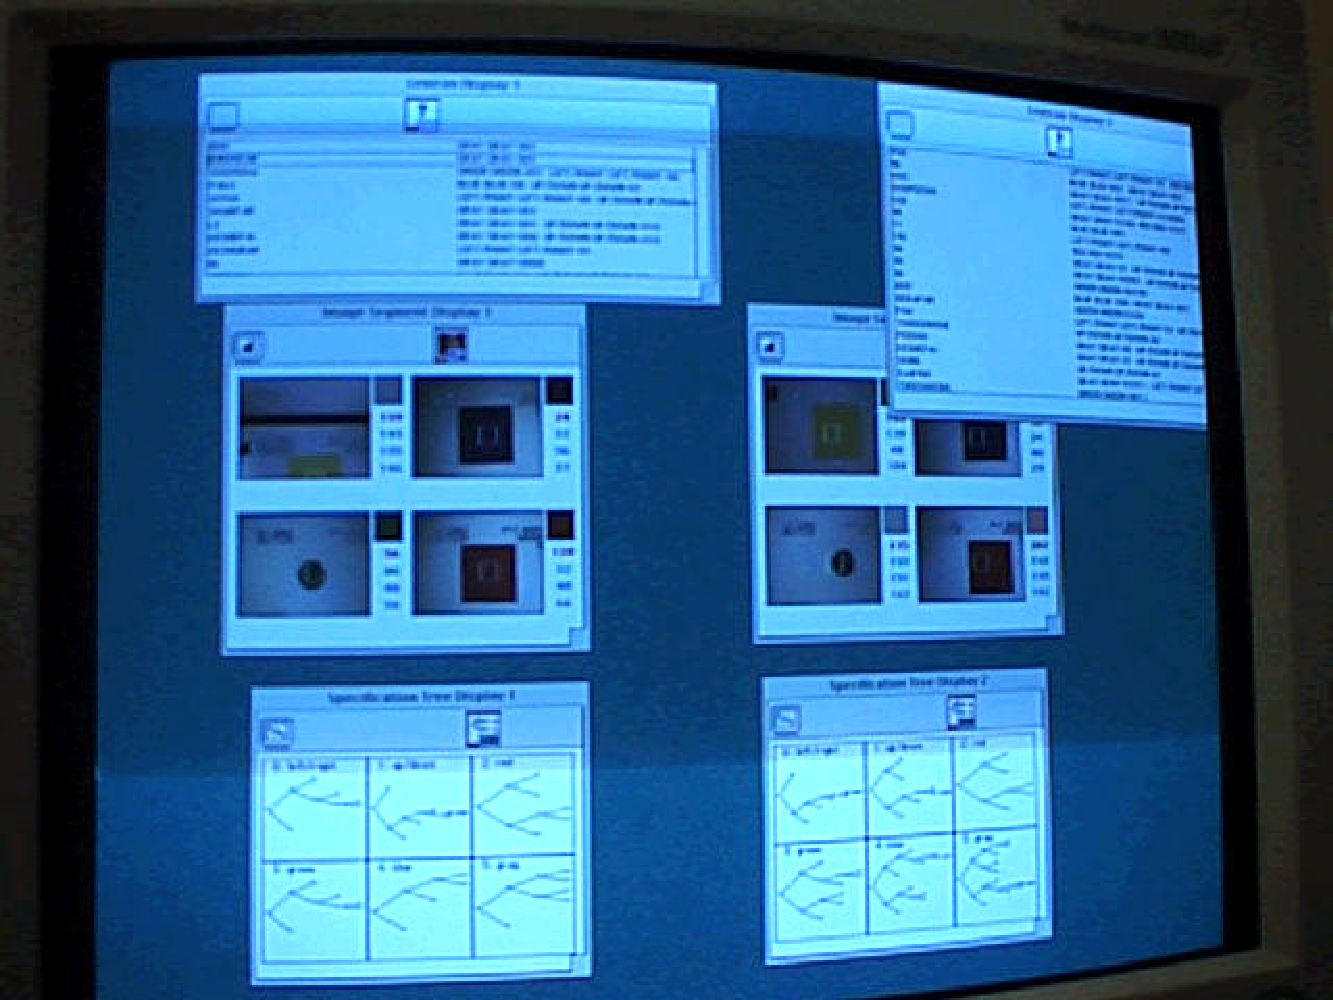
\includegraphics[width=.60\textwidth]{chap1/figs/Interface}}
\caption{ Interface through which the internal states of agents can 
be inspected. Two agents are shown. The top windows show the state of an agent, 
the middle windows the camera inputs that the agent sees and the bottom windows show 
their discrimination trees.}
\label{f:agentview}
\end{figure}

In constructing the robot bodies, we have used as much as
possible off-the-shelf standard 
components so that we could focus almost completely on issues
directly relevant to language and meaning.
Each robot's low-level vision system
(integrated in the camera) is already very sophisticated.\footnote{
The camera is a Sony EVI-D31. The main computer is a Power 
Macintosh from Apple, Inc. The agent servers run under the 
Lynux operating system.}
It can focus automatically to get a sharper image
and autonomously track a moving object. The speech signal is 
produced with a standard text-to-speech system 
so that we did not have to 
worry about building complex audio modules ourselves.
The computer hardware 
is powerful, but not specialised nor in the supercomputer 
range. All programs have been written in the standard symbolic 
programming language of artificial intelligence 
research, namely LISP.\footnote{
The construction of the programs underlying the 
Talking Heads experiment has required advanced
artificial intelligence programming techniques, 
such as discussed by \cite{Norvig:1996}. A general
toolkit for the systematic execution of 
simulation and physical experiments, called BABEL, has been
designed and implemented by Angus McIntyre. The 
toolkit allows the definition and modular composition
of cognitive architectures, the design of 
experiments, and the monitoring and displaying of 
results, \cite{McIntyre:1998}.} What makes the Talking Heads experiment
special is not the hardware or software tools
but what we have done with it.

\subsection{The agents}
\is{agent}

Agents can only engage in interactions with other agents 
when they are physically instantiated
in a robot. Each agent has a basic brain architecture
with different layers performing the cognitive functions 
relevant for playing language games: 
\begin{itemize}
\item A perceptual layer which performs low level signal 
processing to segment the image and collect data about 
each segment such as the colour, size, position or shape
of a segment. 
\item A conceptual layer which categorizes and 
conceptualises the segmented and processed image. 
It is based on a self-generated and evolving repertoire
of categorial distinctions, such as red versus green, or
small versus large. Such a repertoire is referred to as 
the agent's ontology in this book. 
\item A lexical layer which maintains an evolving repertoire
of associations between meanings and words, which I will refer to 
as the lexicon, and performs lexical lookup while parsing 
or producing utterances. 
\item A syntactic layer which uses 
grammatical schemata for organising words
in larger structures or for recognising these structures and
reconstructing complex meanings. 
\item A pragmatic layer which carries out the
scripts for playing language games and maintains the machinery 
for engaging in interactions with other agents in a 
shared environment. 
\end{itemize}
Each of these layers is described in more detail 
later. The internals of the layers are not static but
constantly evolving and adapting. They are not strictly 
modular but coupled in various ways to each other.
Each verbal interaction 
in effect changes the agent's internal state and thus 
influences future behavior. A new, virgin agent 
starts without any built-in ontology, lexicon, nor grammar. 
This is one of the crucial points of the whole experiment, 
because we want to test possible theories on how language
and meaning can evolve and be acquired {\itshape ab initio}. 

Agents are part of populations which determine the probability
with which they encounter each other. This generates 
a dynamic process at two levels: There is the dynamics of the evolving
cognitive competence of each agent (the ontologies, 
the lexicon, the grammar), and there are 
the evolving macroscopic structures which arise in a population
of agents, such as the common lexicons or shared grammars. 
We will see that the mental 
characteristics of agents, even in a single population, are never 
identical because each agent has his own history of 
interactions with the environment and with other agents. 
This is another crucial aspect of the experiment. 
We want to investigate in how far communication is possible
without complete ontological or linguistic coherence. 

\subsection{Interactivity}

To qualify as a sound scientific experiment, anybody 
who wishes to challenge the claims should be given 
the tools `to see for himself'. There are three 
ways in which we have empowered observers to do so. 

First, each physical Talking Heads site has 
a complex infrastructure to organise the interactions between
agents operating in that location, and to support the
arrival and teleporting of agents. This infrastructure also houses
a {\itshape commentator}, a computer program that
monitors the dialogs, inspects the internal states of each
agent, and displays useful statistics such as the degree
of sharing of the lexicon, the competition between different
words to express a particular meaning, the stability of 
certain syntactic constructions, etc. The commentator 
produces spoken or written comments and displays
measurement results on an additional computer screen. 

Second, the teleporting infrastructure makes it possible 
to implement interactions between humans and artificial agents, 
either directly in the shared physical environment or 
through the Internet. At any time, a human experimenter can
pretend to be one of the agents: seize 
a robot, partly control the
camera to set the context of an interaction, and type 
in expressions playing the role of speaker or hearer in 
a language game. The human experimenter can create a 
new, virgin agent, track in detail how this agent acquires the 
categories and language in an existing group, 
or try to influence the currently dominating language
by introducing new words or constructs and following
their propagation (see \figref{f:plate8}). 


\begin{figure}[htbp]
  \centerline{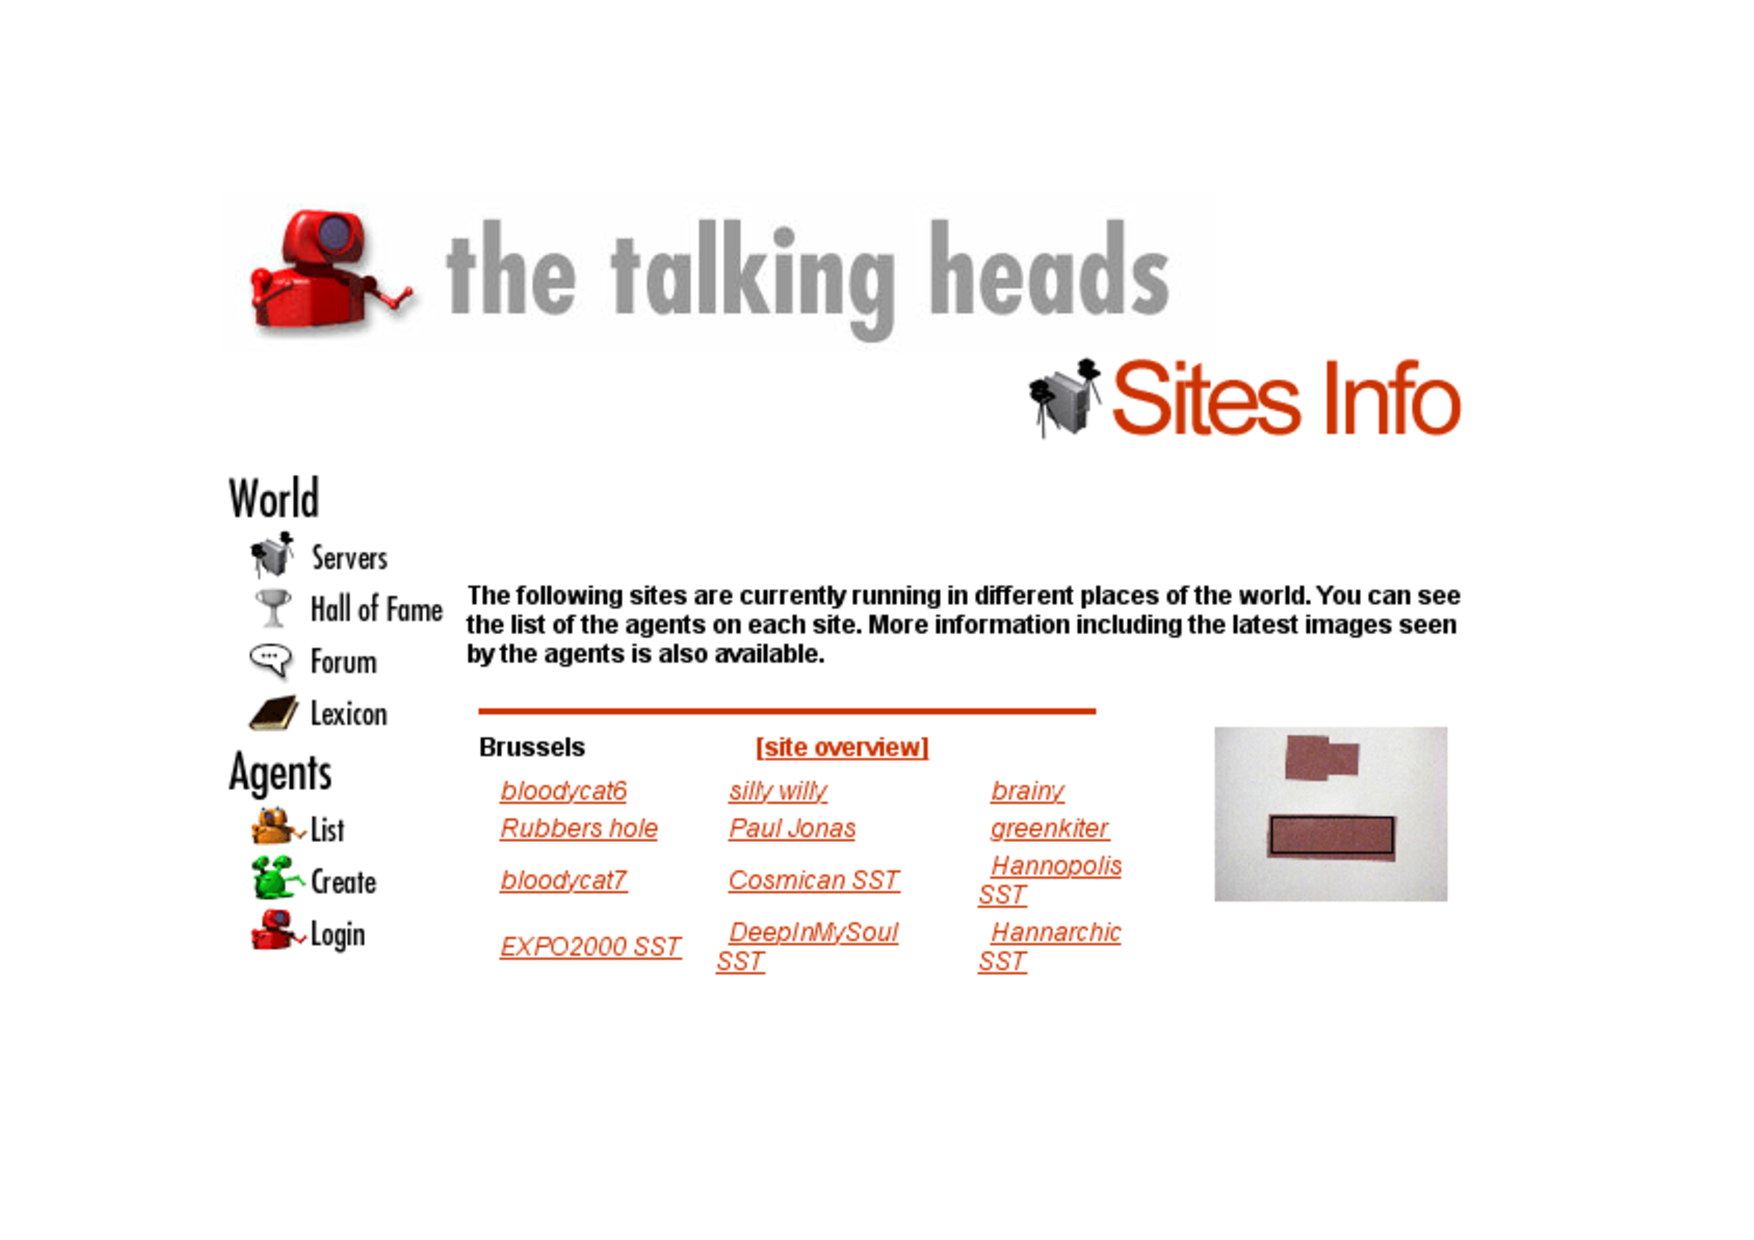
\includegraphics[width=.80\textwidth]{chap2/figs/interface}}
\caption{ Internet interface through which users can 
access the state of games on remote sites and 
follow the experiment.}
\label{f:plate8}
\end{figure}

Finally, the environment has been restricted to 
increase the transparency of experimental results. It 
consists in all locations of a magnetic white board mounted
on the wall in front of the robots (see \figref{f:plate9}). On this
board, the human experimenter can paste various
figures, typically stylised geometric figures like 
rectangles, circles, and squares,
in various sizes, shapes and colours. By changing the 
environment, the experimenter can try to find out what
visual categories the agents employ and force the expansion 
of categorial repertoires, for example by pasting
new types of figures on the board. He can probe the 
adaptivity of the agents by setting up situations that 
destabilise an existing lexicon and see how long it 
takes before a new, perhaps more abstract lexicon emerges. 
All these tools generate unprecedented opportunities to apply 
the most rigid scientific evaluation criteria to the
theories of language and cognition that I will propose in this
book. 

\begin{figure}[htbp]
  \centerline{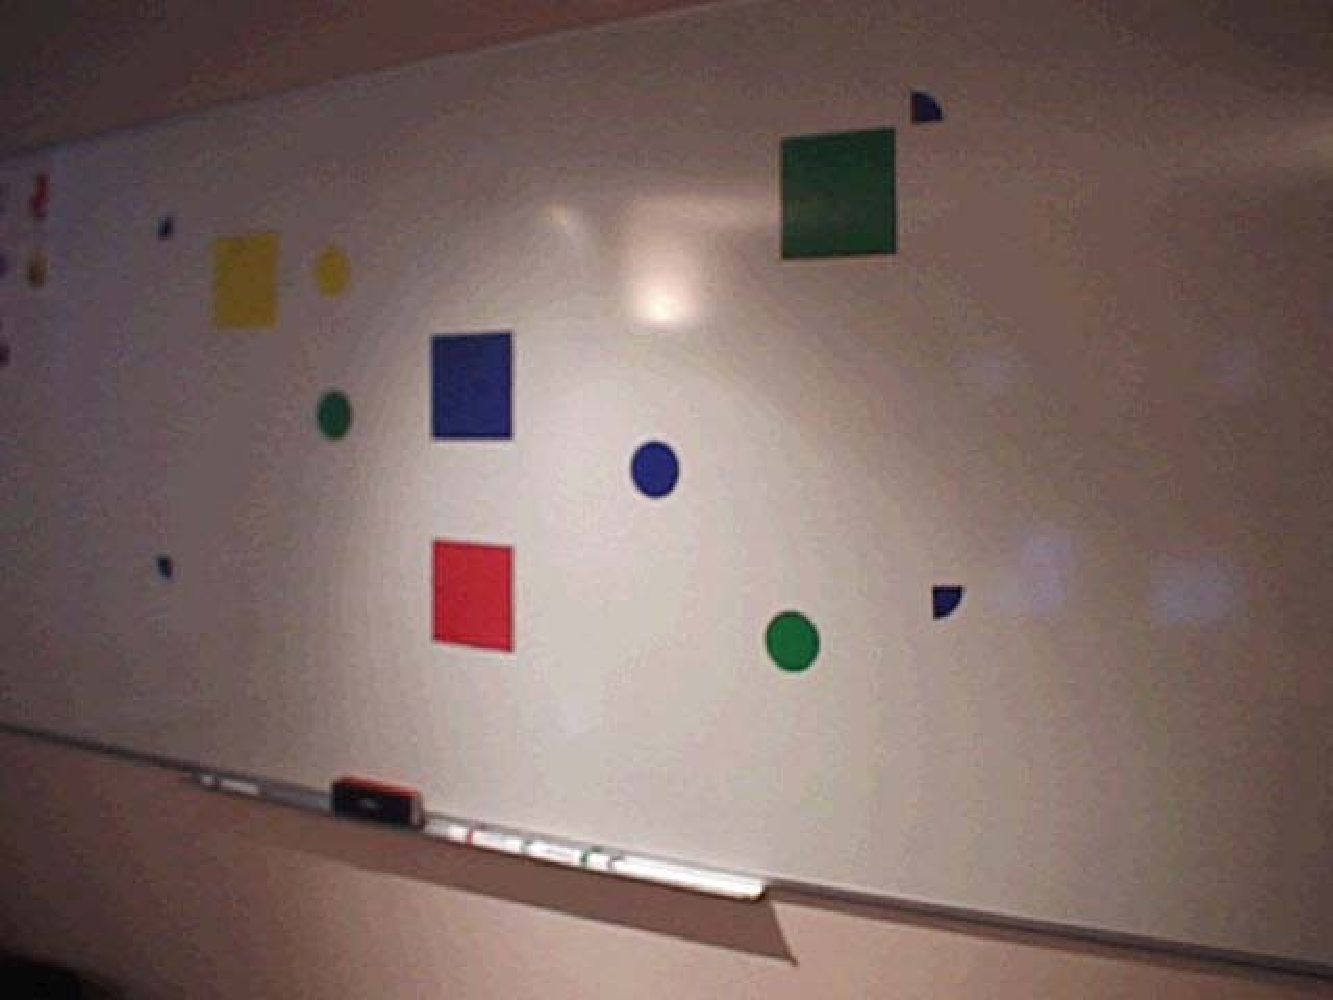
\includegraphics[width=.60\textwidth]{chap1/figs/Whiteboard}}
\caption{ The physical environment of the Talking Heads  
consists of a white board on which various
geometric figures can be pasted. The light conditions were not under the control 
of the experimenters in most locations.}
\label{f:plate9}
\end{figure}

\section{The Guessing Game}

Given this rich computational and robotic infrastructure, many \is{Guessing Game}
specific experiments are possible. 
Each experiment could explore
a particular interaction between the robots, the environment, 
and human observers. In this book, I explore only 
one type of interaction, which I call the
{\itshape guessing game}.\footnote{
A very similar game has been called the original 
language game by \cite{Brown:1973} in the context of
research on child language acquisition. See also 
the thoughtful analysis in \cite{Halliday:1975}. 
Research on child language has inspired the 
agent architectures and behaviors but they should not
be seen as a realistic model of child language acquisition.}
The Talking Heads play this game 
either among themselves or with a human experimenter. 

\subsection{Rules of the game}

The guessing game is played between two 
physically instantiated agents. Agents in 
a virtual state must queue up to have access to one of the 
robot bodies installed in a particular site before
they can play the game. One agent 
plays the role of {\itshape speaker} and the other then plays the 
role of {\itshape hearer}. Agents take turn playing games 
so that all of them develop the capacity to be speaker or hearer.
A human experimenter can pick one of these roles and 
play the game instead of an artificial agent. 

The speaker first looks at one area of the white board and 
directs the attention of the hearer to the same area.\footnote{
I will explain later how exactly agents
decide on a particular scene and how they are able to 
draw each other's attention to specific areas of the 
white board.}
The objects located in this area constitute the {\itshape context}. 
The speaker then chooses one object from the context, which 
I will call the {\itshape topic}, and gives a verbal hint
to the hearer. The {\itshape verbal hint} is an expression
that identifies the topic 
with respect to the other objects in the context. For example, 
if the context contains a red square, a blue triangle, 
and a green circle, then the speaker may say something like 
"the red one'' to identify the red square as the topic. 
If the context contains also a red triangle, he has to be more 
precise and say something like ``the red square'' to delineate
the topic from the non-squares as well as
from the blue square. 
Of course, the Talking Heads do not say ``the red square''
but use their own language and concepts which are not 
necessarily the same as those used in English. For example, 
they may say ``malewina'' to mean [UPPER EXTREME-LEFT LOW-REDNESS]. 

Based on the verbal hint, the hearer tries to guess what
topic the speaker has chosen, and communicates his choice 
to the speaker by pointing to the object. Given that 
the robots do not have arms, pointing is realised by 
focusing on an object. One robot can `see' in which direction another one 
is looking, and thus know where he is `pointing'. 
The game succeeds if the topic guessed by the hearer is 
equal to the topic chosen by the speaker. 
The game fails if the guess was wrong or 
if the speaker or the hearer failed at some earlier point in the 
game. 

In case of a failure, the speaker gives an extra non-verbal
hint to the hearer by himself pointing to the topic, 
and both agents try to repair
their internal structures to be more successful in future
games: The speaker weakens his hypothesis that the words
and constructions he used 
were `right', in the sense of shared by other agents. 
The hearer tries to guess what meanings the speaker 
might have used and deduce what form-meaning relations or 
syntactic constructions he is missing. Pointing by gesturing is
always vague, and the repair actions are far from guaranteed to succeed. 
Nevertheless, they gradually lead (as we will see) to 
a sufficiently shared communication system meaning that 
success in guessing the topic purely based on language
communication increases to reach almost 100 \%. 

\subsection{Nature of the game}

The Guessing Game is one of the common things we do with language. 
For example, I play a similar game when I sit with a friend
at the dining table and say ``could you give me the salt''. 
If she guesses correctly what I mean and hands 
me the salt, the game has succeeded. If she looks at me 
with a puzzled face (maybe she does not speak English) or hands me
the salmon instead of the salt, the game has failed. In that case, 
I can gesture in the direction of the salt and say ``no, no, the {\itshape salt}
please'', and perhaps then she hopefully realises and gives the salt to me. Failure 
is common in natural language dialogs and may be caused by 
many factors. For example, the salmon could indeed 
be close to the salt and my pronounciation of the word ``salt''
may have sounded a bit like ``salmon'', perhaps because there was
loud music playing in the background or perhaps
my friend does not understand English. 
A failure is often 
an opportunity to negotiate how something will be expressed
in the future. For example, the hearer may pick up a new word
or the speaker may realise that a certain word is 
not appropriate in this particular context. 

The guessing game is not a game of winners and losers because both 
agents win or both agents lose at the same time. But it is a game
nevertheless, because it is played with clear rules, 
with a clear outcome and strict limitations on how 
success can be achieved. An agent can not look inside another
agent's brain state. Agents can only interact through the 
external environment. There is no global control 
center that is monitoring the behavior and internal states
of all agents and setting the way they should speak or 
perceive their world. The artificial agents are autonomous and
fully distributed, just like human beings. 

The game is different from a closed world game like 
chess, because the environment is open. The human 
experimenter may introduce new objects at any
time, any one agent can extend
the language (for example invent a new word), possibly
requiring the other agents to adopt it as well, or the
human experimenter may inject new language forms in the 
dialogs. Agents try to maximise their communicative 
success so they cooperate to the fullest and update or change
their internal structures and processes
to improve their chances in the game.\footnote{
The guessing game is a cooperative game, because
both the agents win or loose at the same time and have 
the highest gain if they develop co-ordinated behavior. 
The agent who manages to have most success in the game is 
the global winner. Because the commentator requires to know 
from the speaker which topic he wants to communicate 
before he is allowed to speak, no cheating 
is possible. Game theory, originally founded by 
von Neumann and Morgenstern, can be applied to study the 
language game mathematically. \is{game theory} We are dealing with an 
evolutionary game in which the players optimise their 
internal states to become better in the game 
\cite{Maynard:1982}.}

In the Talking Heads experiment, it is assumed that 
agents want to cooperate and that they use communication
as part of their cooperation. 
The evolution of cooperative games has been studied 
extensively by artificial life researchers often 
in the context of Axelrod's prisoners dilemma game,\is{prisoners dilemma game} 
see for example: \cite{Ikegami:1994} 
For a general introduction how communication can 
evolve in the context of cooperation, see: \cite{Hauser:1996}. 
Computer simulations showing the evolution of 
cooperation and communication have been reported in the
artificial life literature. See for example: \cite{MacLennan:1991} 
Most of these computer simulations are 
closer to animal signaling systems than to human lexicons
both in size and in terms of the complexity of meaning.

The guessing game is clearly not the only thing we do 
with language. Humans are capable of playing a whole 
range of language games and inventing
new ones when the circumstances
require it; however, to do controlled experiments we need
to limit ourselves. The objective of the Talking Heads
experiment is not to cover the full range and complexity
of human natural language interaction but to examine with
objective precision a limited number of issues concerning
the nature of language and meaning. 

\subsection{The semiotic square}

The environment of the Talking Heads is 
not fixed. The human experimenter 
may change the position of objects, add new kinds of 
objects, or eliminate
others. Consequently a strategy of naming individual objects
will not work. It would lead to a proliferation of 
proper names and it would require the Talking Heads to
recognise objects, which is very difficult to do.\footnote{
For a thorough exposition of the difficulties of 
object recognition, see \cite{Ullman:1996}
Object constancy comes fairly late in the 
acquisition of a child's ontology, as Piaget's conservation
experiments have shown. Language probably plays an important
role in forming the notion of an object.}
Indeed, humans don't exclusively use proper names in 
natural language conversations 
either. We say ``could you give me the red small square'' as 
opposed to ``could you give me $O143$". Natural language 
words like ``red'' or ``small'' name perceptually grounded categories
and syntactic structures indicate how they should
be combined and used to find the topic. The relation between 
a language expression and its referent is therefore 
always indirect. This is summarised
in the semiotic square (\figref{triangle}), which I will use throughout this book to 
help understand and analyse the nature of language communication. \is{semiotic square}
The semiotic square relates the four entities
involved in a verbal interaction: 
\begin{itemize}
\item An {\itshape utterance}, such as ``small red square'', which is 
transmitted as a physical 
signal from one agent to another one through the 
external environment. It is written between double quotes. 
\item A {\itshape meaning}, which consists of categories like [RED], [SMALL], 
or combinations of categories, like \{[RED] [SMALL]\}. Labels of 
categories are written in capital letters between 
square brackets. 
\item An {\itshape image segment}, denoted as $S143$, which is 
a segment of the image perceived through the camera.
\item A {\itshape referent}, like object $O143$, which is 
an entity in the real world. 
\end{itemize}


\begin{figure}[htbp]
  \centerline{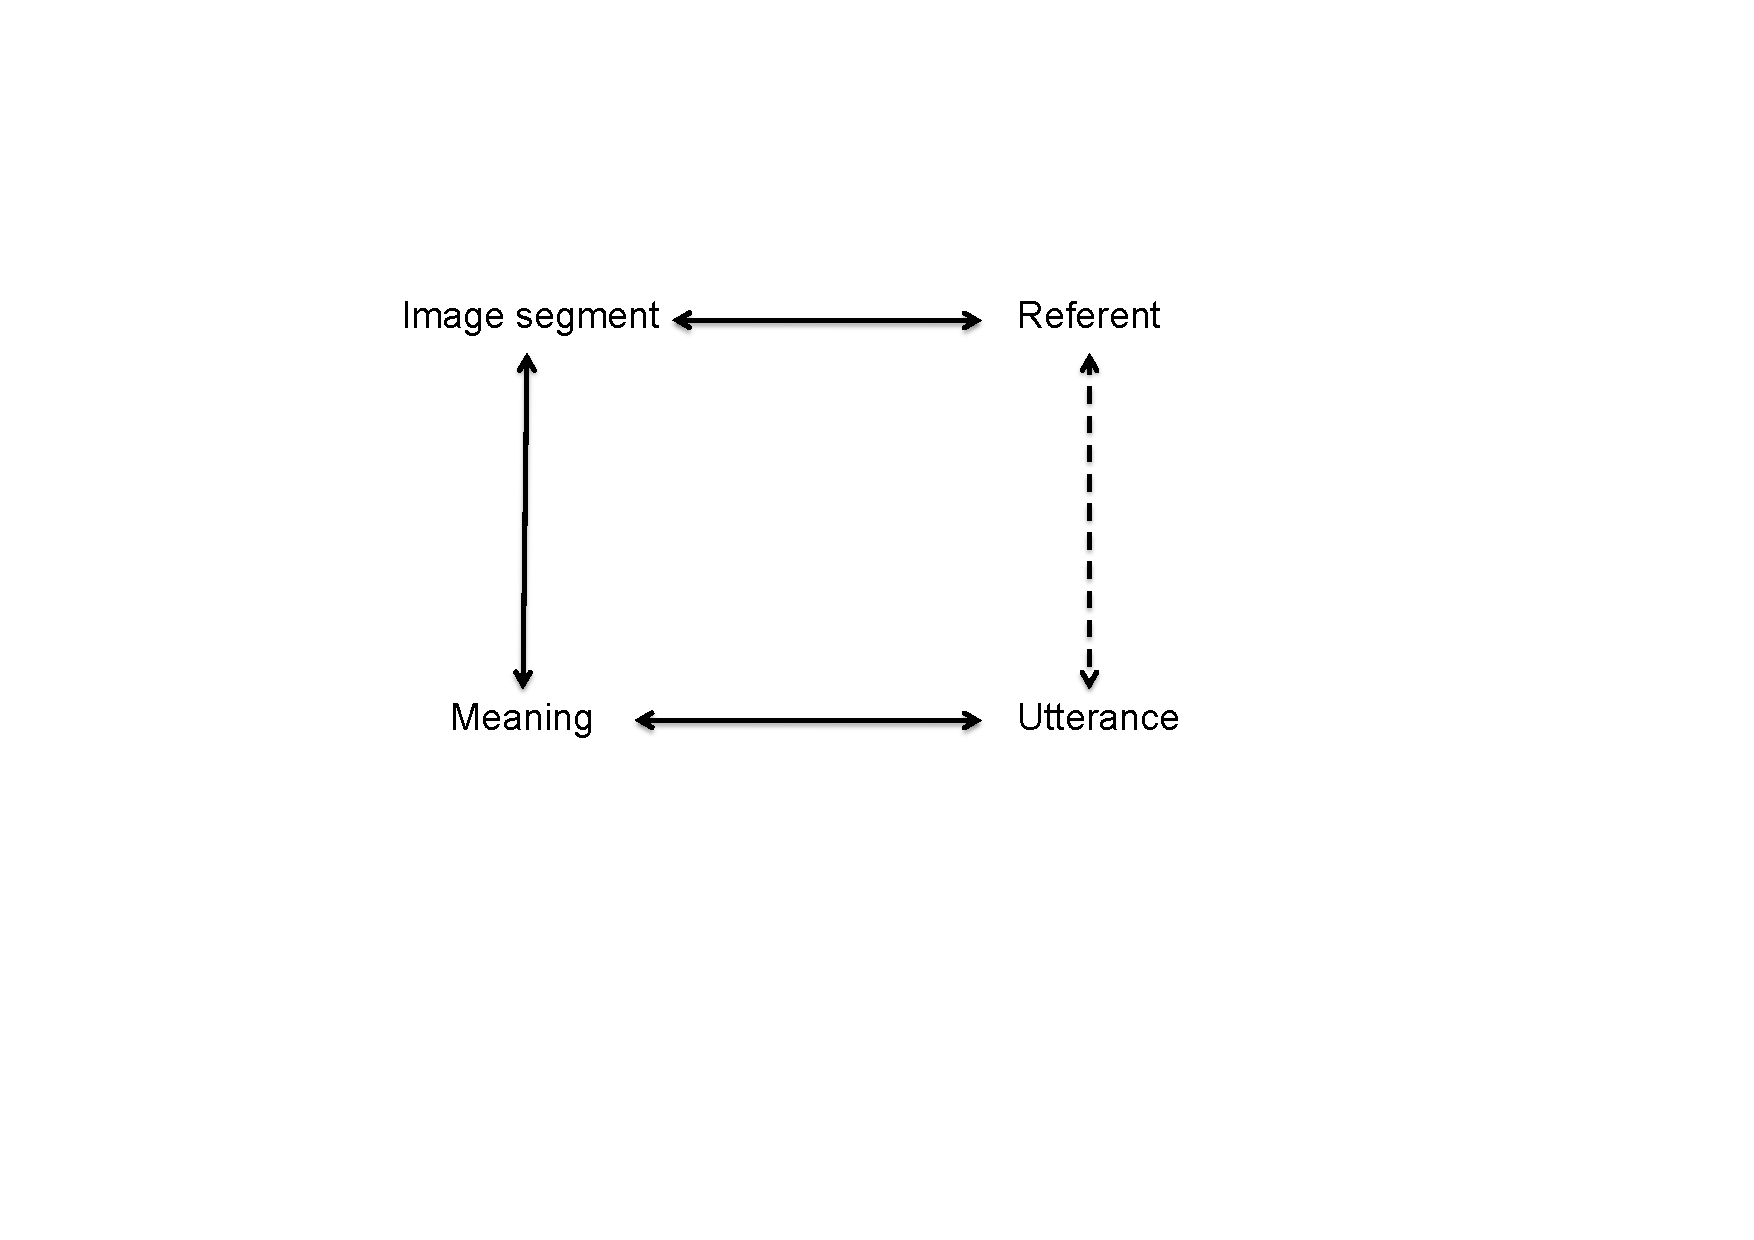
\includegraphics[width=.65\textwidth]{chap2/figs/triangle}}
\caption{\label{triangle} Any verbal interaction
involves four entities here grouped in the
`semiotic square'. The relation between utterance
and referent always needs to be established indirectly by 
passing through perception and meaning.}
\end{figure}

The systematic relation between meaning and referent is 
usually studied under the heading of semantics, and the 
systematic relation between meaning and utterance as
grammar (including syntax, morphology and lexicon).\footnote{
For a general introduction to the contemporary linguistic
viewpoint on the processes involved, see: \cite{Vanvalin:1997} 
In a logical approach to language, as 
exemplified by Montague grammar \cite{Montague:1974},  
meanings are represented using a logical formalism, i.c.
a variant of intensional logic. \is{Montague grammar}
Natural language expressions are systematically 
related to expressions in this logic, and a
formal semantics system defines how expressions in the logic
are mapped onto their denotations. Because this is 
a formal framework, the denotations consist of formal 
models. To make the Talking Heads experiment work, 
we needed to develop a grounded semantics system, which details
how an agent may go from physical reality to meaning
using a perceptual apparatus, and from meaning 
to physical reality. The logical structure of 
the meanings we will investigate are very simple 
(unary predicates and conjunctions). But once we know how to 
set up a grounded semantics for simple meaning
structures we can scale it up to the more complex meaning
structures typically studied in logic.}

Many tricky philosophical issues are raised in 
the unavoidable distinction between the sensed image
of an object (which is local to the agent)
and the object itself (which is external to the 
agent). Some philosophers even doubt that objects 
have an existence outside our perception of them! 
We need to make the distinction because agents always
have different internal images even if they look at 
the same object seen from our viewpoint as an external
observer. However, for simplifying the 
explanations, I will sometimes assume that perceived
image and external object are the same, so that the 
semiotic square becomes a semiotic triangle.\footnote{
The notion of a semiotic triangle was first
introduced in a classic of the semiotic literature, 
see \cite{Ogden:1935}.}

When we put together the semiotic squares of two 
agents (\figref{triangle2a}), we see more clearly 
that agents are trying to agree about a common object
in the external word, but they never have 
any direct access and hence confirmation whether they 
are really referring to the same object. 
Only through pointing or other
cooperative actions can speaker and hearer co-ordinate
whether they indeed refer to the same object in
the external reality. 

The utterance is not the same for both agents, because it
needs to be articulated, transmitted, and perceived through 
a physical medium. Errors in transmission or perception may 
and do occur and have an important impact on the evolution of 
language. To remain focused, I will not really treat this issue in 
this book but will instead assume that there is direct, error-free transmission
of the utterance. 

\subsection{Processes involved in language communication}

I will use the following terms for denoting the 
processes speakers and hearers go through while traversing
the relations in the semiotic square as they play a language
game (\figref{triangle2a}). 
A similar framework, but emphasising the 
language production side, has been described in great
detail by \cite{Levelt:1989}. That book also provides a wealth
of psychological evidence that these processes must 
be going on and expands the phonetic and phonological 
side. An example of a detailed architecture inspired by 
generative grammar is discussed in: \cite{Jackendoff:1997}. 
Generative approaches to language attempt to define a language by 
generating its set of possible utterances. Interpretations
are constructed from the syntactic structure derived by 
the generative grammar. In this book, we are interested 
in the mapping from communicative intent 
in a perceived reality to an utterance and back. The knowledge
and skill needed to solve this problem is different from 
that need to systematically generate the set of sentences in a 
language and their possible interpretations.

1. The speaker as well as the hearer {\itshape perceive} reality
by capturing an image through the camera, segmenting 
the image into coherent units, and deriving various 
sensory characteristics about each image segment, 
such as the colour, size, movement. 

\begin{figure}[htbp]
  \centerline{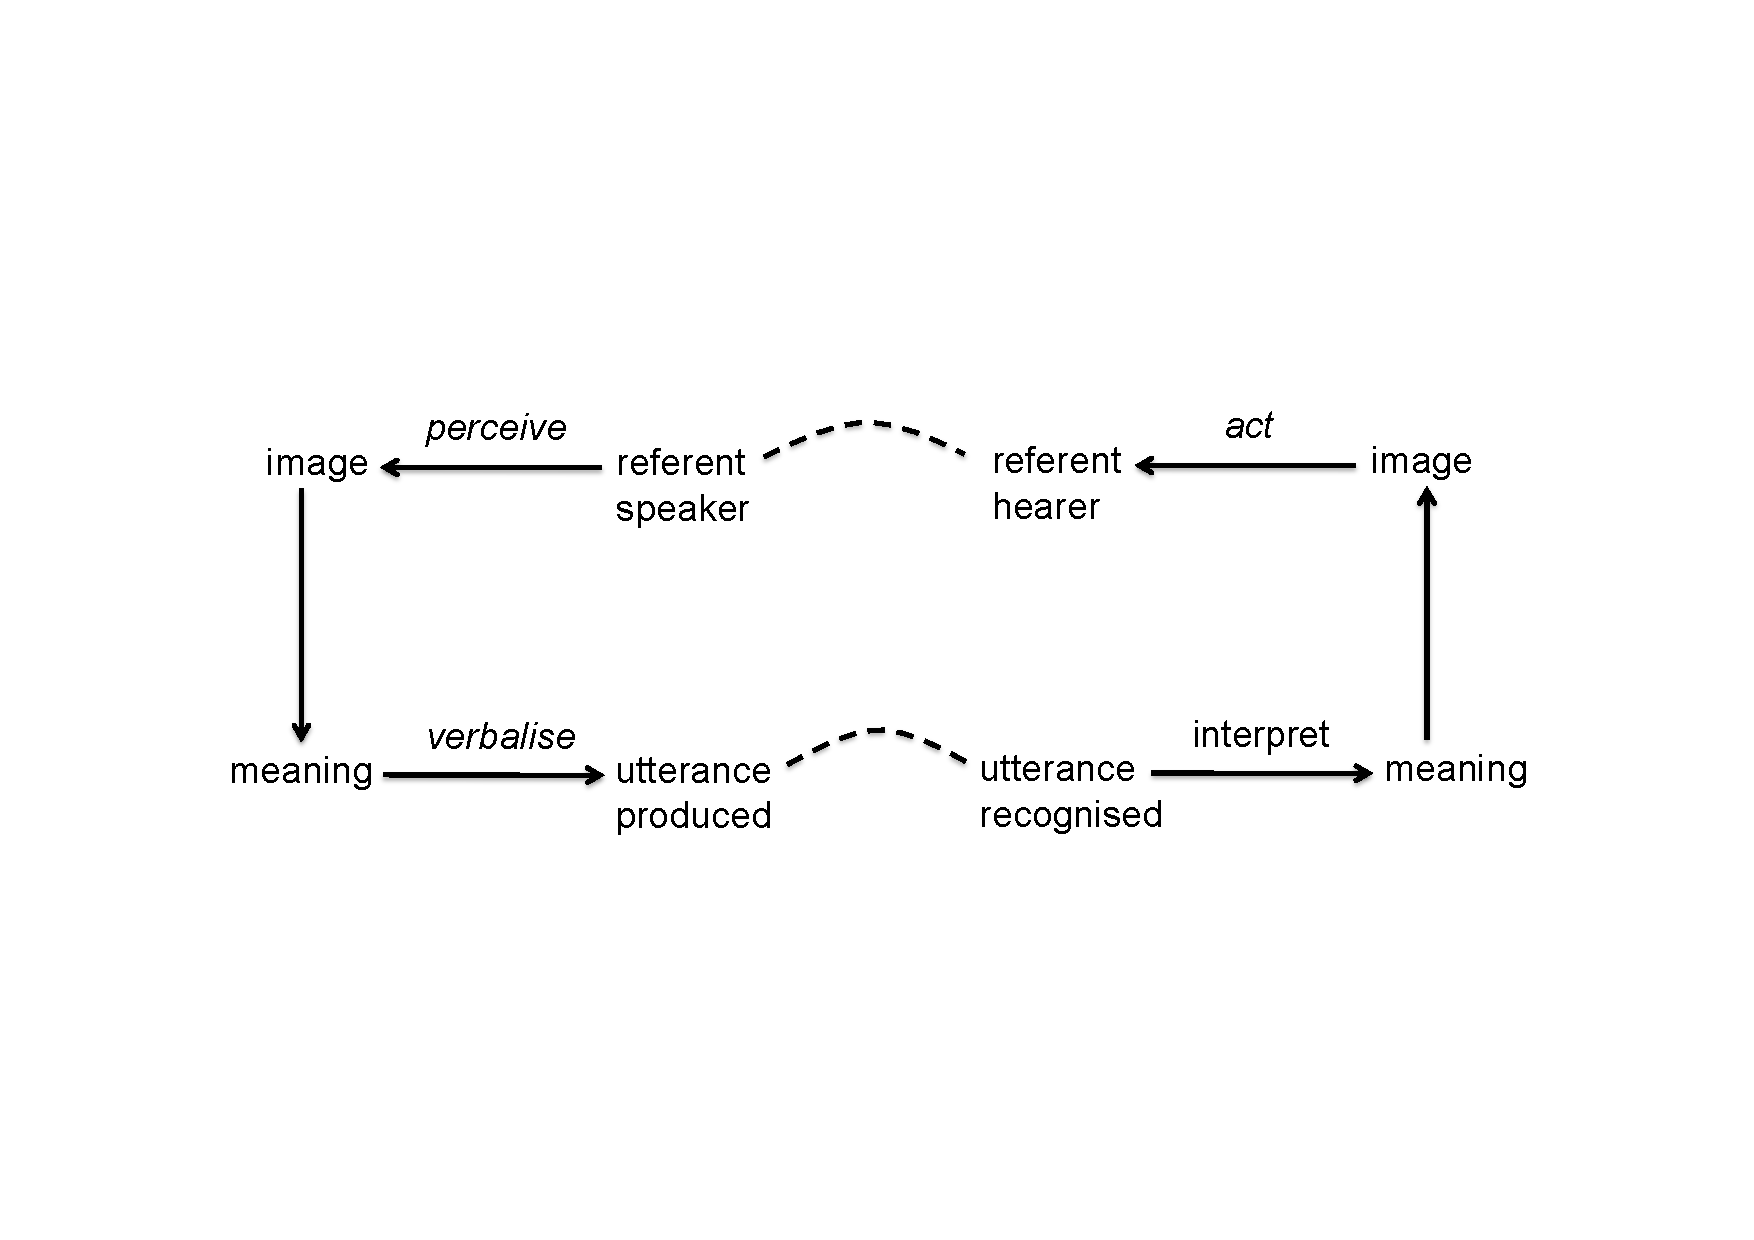
\includegraphics[width=.85\textwidth]{chap2/figs/triangle2}}
\caption{\label{triangle2a} Left: processes carried
out by the speaker. Right: processes carried out by the hearer.
There are also feedback processes moving in alternate directions
until the agents settle on coherent choices for all the items
in their semiotic squares.}
\end{figure}

2. The speaker must then {\itshape conceptualise} the 
scene on the basis of this perception. He must find a set of
categories or a conjunctive combination of 
categories that distinguishes the referent from the other objects in 
the context, and which will act as the meaning of 
his communication. For example, he might choose [BLUE] if the
topic has a blue colour and all the other objects in the 
context are not blue. 

3. The speaker must then {\itshape verbalise} this conceptualisation. 
He must use his language system to find words and 
syntactic constructions expressing this meaning.
For example, he might choose ``blauw'' (if he speaks
Dutch), or ``bleu'' (if he speaks French),
to convey the category [BLUE]. 

4. The hearer must engage in similar tasks but now
going in the reverse direction. He must
{\itshape interpret} the utterance to find out which
conceptualisation constitutes the meaning. 

5. Then the hearer must {\itshape apply} this meaning
to see what referent was intended. The hearer has
also perceived the scene in terms of a set of 
segments and now uses 
the meaning to identify the segment that
could have been the one intended by the speaker.

6. Finally the hearer {\itshape acts} upon the outcome of meaning
application. He points to the topic he has identified. This is the 
step where both agents co-ordinate their 
behavior through the external world. 

\subsection{Knowledge sources and competences}

Each of these activities requires knowledge and/or skill
(summarised in the table below). Perceiving requires 
visual processes capable of segmenting images and deriving image 
segments. Conceptualisation requires an {\itshape ontology}, 
a repertoire of perceptually grounded distinctions
that can be applied to a segmented image to yield 
distinctive categories or category combinations that 
may constitute the meaning of the utterance. Verbalising 
a conceptualisation requires 
a {\itshape lexicon} that maps parts of the meaning to words and 
a {\itshape syntax} that specifies how to organise individual words
into a larger complex. 
The hearer must use similar 
knowledge sources in the other direction. He must use 
his lexicon and syntax to reconstruct the meanings expressed
by the utterance, and then use the 
ontology again to apply the meaning to the present 
context to find the referent \tabref{tab:2:findthereferent}. 


\begin{table}[htbp]
\caption{}
\label{tab:2:findthereferent}
\begin{tabular}{ l  l  l  l }
\lsptoprule
{\itshape Activity} & {\itshape From} & {\itshape To} & {\itshape Knowledge source}\\ \midrule
Perceive & Object & Image segments & Visual processes \\ 
Conceptualise & Topic & Meaning & Ontology  \\ 
Verbalise & Meaning & Utterance & Lexicon + syntax \\  
Interpret & Utterance & Meaning & Lexicon + syntax \\ 
Apply & Meaning & Topic & Ontology \\ 
Act & Topic & Object & Behavioral process  \\ 
\lspbottomrule
\end{tabular}
\end{table}

I do not want to suggest that there is a simple linear flow 
neither from perception to utterance nor from utterance to 
perception. Instead, we must imagine a dynamic process 
involving forward and backward propagation of information 
until coherent choices for all the nodes in the two
semiotic squares have been established by the speaker and 
the hearer. Many different choices are initially possible 
(many segmentations, conceptualisations, verbalisations, 
interpretations) but the dynamic process gradually settles into 
a single coherent attractor, so that speaker and hearer 
agree upon a common referent. The co-ordination between 
chosen topic and identified referent is done through 
the real world (pointing, handing an object, performing
an action). 

I deliberately left an important aspect of language out. 
In the case of physical agents, the form cannot be transmitted
directly but needs to be articulated in speech sounds, 
written signs, or gestures, to create a true utterance. This additional 
complexity will not be discussed further in this book - even though 
it is a fascinating topic in its own right.\footnote{
See for a state of the art review: \cite{Clark:1990}
We have already been conducting quite extensive 
research in our group on the origin of sound systems 
using similar principles as the ones discussed in this 
book for the origins of word semantics. 
See: \cite{DeBoer:1997} The complex 
adaptive systems approach underlying this phonetics
work was already foreshadowed in work of phoneticians
like Bjorn Lindblom \cite{Liljencrants:1972}.}
To make a verbal interaction nevertheless complete, agents
are given a repertoire of consonants and vowels with 
which they can make random syllables and syllable combinations, 
like ``wabido'', ``bimaku'', etc. The articulation and 
recognition of these syllables is assumed to be acquired
already and transmission is engineered to be error-free. 
This way, our attention can be focused on how
ontologies, lexicons, and grammars may emerge. 

\section{Perception and categorization}

I will now discuss in some more detail each of the processes
the Talking Heads go through when they 
play a complete language game, leaving a more detailed 
discussion to subsequent chapters.

\subsection{Scene and topic selection}

Every physical Talking Heads set-up features a `waiting room' in 
which agents are stored, ready to be loaded into the 
robotic infrastructure or to be teleported to another
physical site. A game starts when two agents are chosen
at random from this waiting room and loaded into 
the two physical robots. The
internal architecture of each agent is connected with 
the sensori-motor apparatus of the robot so that they can 
receive the sensory data streams recorded by the camera
and control the movements of the robots. Then the general 
control system assigns randomly the role of speaker and hearer
to each of the agents and the game can begin. 

Next the speaker randomly moves around its camera, halts 
at a particular location, and captures
the image. The speaker then attempts to segment 
this image. If the scene is `interesting', which means that
there are at least two clear segments, it is chosen 
for playing a language game. Otherwise the agent makes another 
random movement and repeats the process. An example of 
an interesting scene with its subsequent segmentation
by the speaker is shown in \figref{f:plate10} (top image on the right). The scene
has two circles as main objects. Segments which are too 
small are ignored. 


\begin{figure}[htbp]
  \centerline{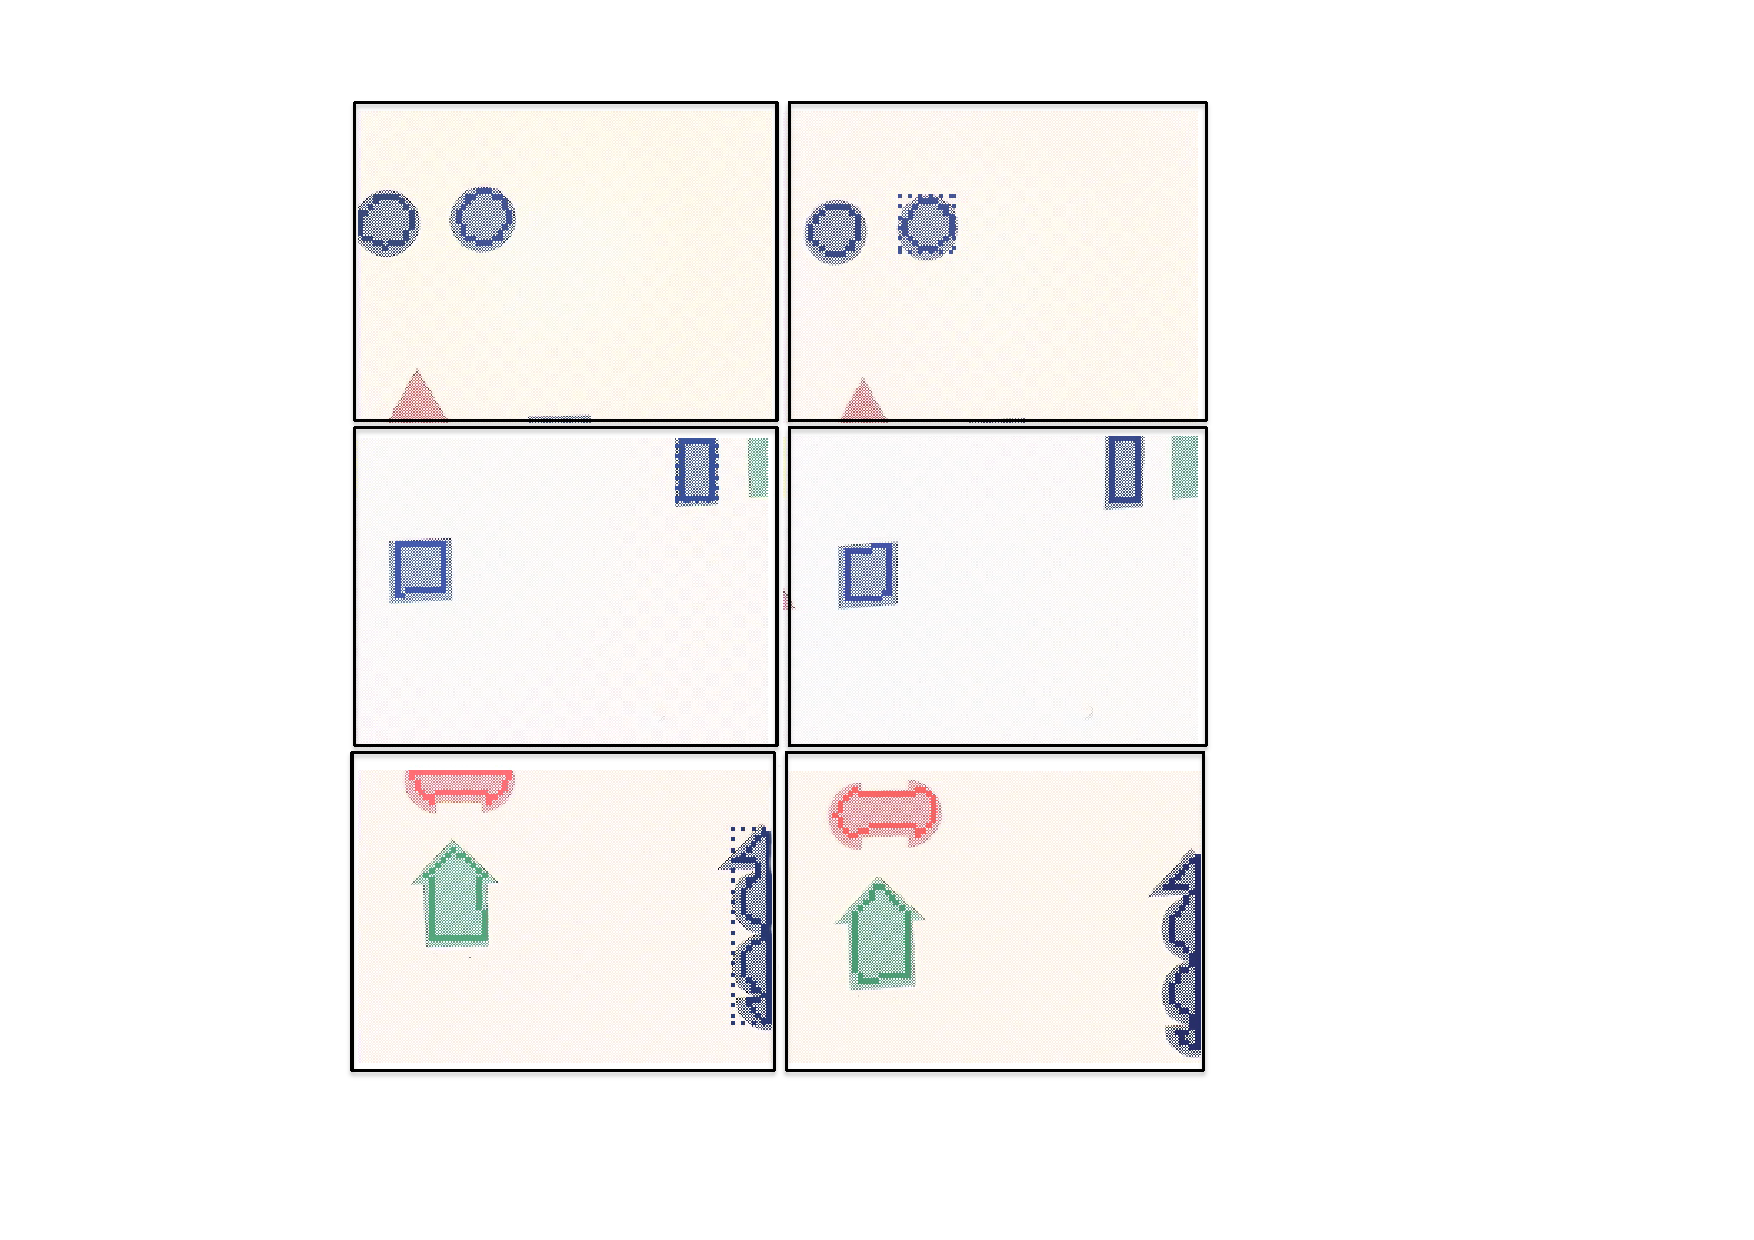
\includegraphics[width=.60\textwidth]{chap2/figs/hpos}}
\caption{ Three examples of segmented images (from top to bottom). Left and right images 
show the perceived and segmented images for two agents respectively. These images are always
different because they are dependent on the position of the agent. 
The topic is indicated by a dashed bounding box in the 
image of the speaker (on the right for the first case and on the left for the others). 
Segments which are too small are ignored. The topics have all been conceptualised
as being `to the right' and so the same word 
``gofubo'' has been used to successfully refer to them.}
\label{f:plate10}
\end{figure}

Segmentation can happen according to several criteria. \is{image segmentation}
For example, patches with similar colour can be grouped 
into a single patch, edges can be identified 
and then linked with each other to form line segments
circumscribing the contours of 
an object, or consecutive images can be compared to extract the parts
that changed and hence moved as a single object. 
There is now a solid body of techniques from decades
of machine vision research to efficiently segment scenes according to 
these and other methods. The Talking Heads use several methods
in parallel and combine their output to get a clearly segmented
picture.\footnote{
For general introductions to these areas, 
see: \cite{Ballard:1982} and \cite{Fischler:1987}}

The hearer must be able to sense in which direction the speaker is looking. 
This facility is at the moment implemented by having 
the speaker indicate to the hearer the point on the white board 
at which its camera is focused. The hearer then moves the camera
to this point and records an image as well. The hearer segments 
this image (see \figref{f:plate10}, top image on the left) so that 
now both the speaker 
and the hearer have a set of segments and can start playing 
a language game. Note that the speaker and hearer never get 
exactly the same image because they are standing about one 
meter apart from each other before the white board. Also the
calibration is never entirely accurate so that perceptual 
differences are unavoidable.

\subsection{Sensory Channels}

Next low level visual processes gather information about each \is{sensory channels}
segment, such as its average colour, size, shape,
the position with respect to horizontal or vertical axes. 
Each process outputs its information on a {\itshape sensory 
channel} scaled between 0.0 and 1.0. The mechanisms from 
the conceptualisation layer that subsequently use this information
can operate on any kind of sensory channel. 
I will assume for the rest of this chapter that the low level
routines produce each only three types of information, sent
on the following sensory channels: 
\begin{itemize}
\item The first channel is called HPOS (horizontal position). 
It contains the x-midposition of a segmented object within
the field of view of the robot. 
\item The second channel is called VPOS (vertical position). It
specifies the y-midposition of the segmented object. 
\item The third channel is called GRAY and contains 
the average gray-scale of the object. 
\end{itemize}
Later on additional channels will be introduced. 

Consider the two objects in \figref{scene1-1}. The triangular
object has the (scaled) values HPOS=0.35, VPOS=0.40, GRAY=0.33, and 
the rectangular object has the values HPOS=0.70, VPOS=0.85, 
GRAY=0.33. The agents can already visually distinguish
millions of possible scenes with these three sensory
channels. The number of scenes
quickly grows when the set of sensory channels increases. 

\begin{figure}[htbp]
  \centerline{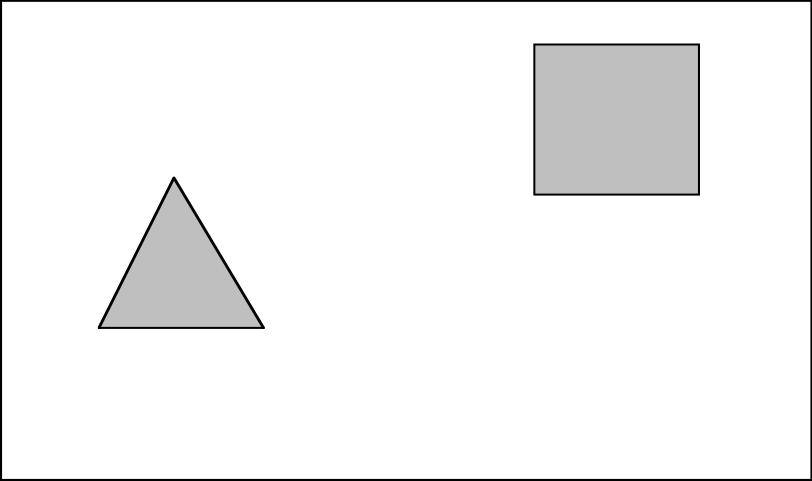
\includegraphics[width=.50\textwidth]{chap2/figs/scene1-1}}
\caption{\label{scene1-1} The scene contains two 
objects: a triangular object and a rectangular object
with the same gray levels. 
Each one is characterised by values on three sensory 
channels: HPOS, VPOS, and GRAY.}
\end{figure}

The low level visual processes outputting
values on the various sensory channels are already quite
complicated in themselves. I will discuss them further in 
chapter 3. I will then argue that the 
agent's repertoire of visual processes does not have to be
static and programmed in advance but evolves and adapts
through a selectionist process. New processes may `grow'
by the random combination of primitive operations and are
pruned when they fail to yield useful information or information 
which is irrelevant in the environment in which the agent 
finds himself. 

\subsection{Making Distinctions}

The data on sensory channels are values from a continuous domain
(between 0.0 and 1.0). 
To be the basis of natural language communication, these
values must be transformed into a discrete domain. This is 
precisely the task of the conceptual layer. It 
performs massive data reduction to make infinitely
rich environments managable. One means of categorization
is to divide up each domain of values on a particular
sensory channel into regions and 
simply assign a category to each region, thus creating a 
discrimination tree.\is{discrimination tree} For example, 
the HPOS-channel can be cut in two halves leading to a 
distinction between [LEFT] ($0.0 \leq HPOS < 0.5$) and [RIGHT] 
($0.5 \leq HPOS \leq 1.0$). The triangular object 
in \figref{scene1-1} has the value HPOS=0.35 
and would therefore be categorized as [LEFT]. Similarly, the 
VPOS-channel can be divided in two halves yielding the 
categories [LOWER] and [UPPER], and likewise the GRAY-channel
yielding the categories [LIGHT] and [DARK]. 
Given these categories, 
the rectangular object in the scene of 
\figref{scene1-1} would be categorized as [RIGHT UPPER LIGHT].
Of course, light, dark, left, lower, etc. are labels 
that I have given to these categories. The Talking Heads 
create categories by partitioning sensory channels but do
not use these labels internally. 

It is always possible to refine a distinction by further
subdividing its region. Thus an agent could further divide the 
bottom region of the HPOS-channel (categorized as 
[LEFT]) into two subregions [TOTALLY-LEFT] ($0.0 \le HPOS < 0.25$), 
and [MID-LEFT] ($0.25 \le HPOS < 0.5$). The triangular object
can now be categorized as [MID-LEFT], if simply categorising it
as [LEFT] is not distinctive enough. Each of these categories can 
still be further refined. The categorisation networks
resulting from these consecutive binary subdivisions form
discrimination trees (\figref{tree1}). It is not at
all assumed that all agents have the same trees; due to 
different developmental histories, divergence is inevitable. 

\begin{figure}[htbp]
  \centerline{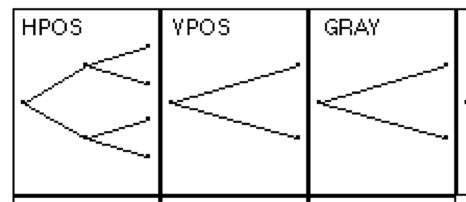
\includegraphics[width=.35\textwidth]{chap2/figs/tree1}}
\caption{\label{tree1} A discrimination tree displays
the divisions of the total range of 
values on a sensory channel into finer and finer subregions. 
Categories are assigned to each region at different 
levels of the tree.}
\end{figure}

There are obviously other ways to 
move from the continuous domain of sensory channels to 
the discrete domain of categories.\footnote{
See: \cite{Taylor:1989}}
For example, it is not really necessary 
to have a binary division, we could just as well split 
each region into three or more subregions. Or we could introduce
focal (prototypical) values and associate
a category with each of them. In the latter case, 
the categorisation process consists 
in identifying the prototype that is closest to 
an object's value. For the current experiment, I will stick however
to a binary categorisation strategy because that is
the simplest to understand and formally investigate. 

We will see that agents build hundreds,
even thousands, of categories as they play their
language games, and in addition they make combinations of 
categories. To bring some order in this profusion of 
categories, I will label them using the 
sensory channel from which a category operates, 
followed by the upper and lower bound of the region they 
carve out. Thus [TOTALLY-LEFT]
is labeled as [HPOS 0.0-0.25], because it carves 
out a region between 0.0 and 0.25 on the HPOS-channel. 
When it must be emphasised that 
a category belongs to a particular agent, for example {\bfshape a1}, we
write [HPOS 0.0-0.25]$_{\mathbf a1}$. The same category in agent {\bfshape a2}
is labeled as [HPOS 0.0-0.25]$_{\mathbf a2}$. If I want to talk about 
this category in the abstract, I will not mention any 
agent and simply write [HPOS 0.0-0.25]. We will also 
allow conjunctive combinations of categories which will be
written as a set, as in \{[HPOS 0.0-0.25], [VPOS 0.0-0.25]\}, 
which could be paraphrased as totally-left {\itshape and}
totally-down.  

Where do an agent's discrimination trees, and hence
categories, come from? This is one of the main 
puzzles to be addressed in this book and it will 
occupy most of chapter 4. Very briefly, 
I propose again a selectionist approach, as for
the formation of low level visual routines. I hypothesise
that the nodes and branches of the discrimination trees
grow more or less randomly in all directions. The use and
success of categories is monitored and categories which 
are not sufficiently useful or successful in the environments
encountered by the agent are pruned. I will argue in chapter 4
that this mechanism indeed leads to 
a repertoire of distinctions that is adequate for 
playing language games, and that 
categories therefore need not be innate nor learned by 
induction from a large series of examples. 

\section{Lexicalisation}

Verbalisation (mapping meaning to form) 
involves two distinguishable activities. \is{verbalisation} The first one
relies on a lexicon to map components of meaning to
individual words. The second 
one relies on syntactic rules to provide supra-word structuring 
and additional syntactic marking to express additional
aspects of meaning, particularly how component meanings
are combined into a complex whole. Both types of 
activities also take place in interpretation (mapping form to meaning):
the individual words are mapped back to their meanings
and the meaning of the whole is reconstructed from the 
meaning of the parts. 

In the early origins of language,
there must have been an initial phase in which no complex syntax 
was in place yet. Utterances then must have consisted of single words
or multiple words without further syntax. \is{proto-language}
Such syntax-less languages have been called {\itshape proto-languages}.\footnote{
See \cite{Bickerton:1990} as well as \cite{Thomason:1988}. Children similarly 
go through a single word phase (even though a single 
word for them might be multiple words for us), and 
then slowly start to bootstrap their grammar. 
See: \cite{Tomasello:1991} and \cite{Bates:1991}. 
They are still observed in the very first phases of 
child language acquisition or in pidgins that spontaneously 
form when two communities with widely diverging languages
need to interact. Out of proto-languages, languages 
with a fully-fledged syntax must have emerged at some point. 
How this occurred is still a heavily debated mystery. In this volume 
I only treat the origins of proto-languages.} 

Children acquire their first words around the first year
of life.\footnote{
Representative work in the study of child language
learning focuses mostly on the acquisition of specific meanings.
See: \cite{Gleitman:1994}, 
\cite{Clark:1993}, \cite{Bowerman:1996}.}
Most people believe that they do this 
as a result of hearing a particular word repeated several times in a
certain context and gradually abstracting an
association between a word and a meaning. But 
how is it that they know which meaning to associate with a 
particular word? How is it that word acquisition goes
so rapid? We will follow a different 
approach, which leaves an open question whether
this applies to human word acquisition as well. The
approach will be selectionist. The agents {\itshape construct} 
hypotheses, either on the basis of one specific case 
where they guess through a non-verbal strategy what 
the meaning of an unknown word might be, 
or they have simply invented a new word because
they do not have one yet. The hypotheses are 
then tried out in subsequent games and either receive confirmation
or are falsified. As a side effect of this local behavior, 
a global self-organising dynamic process arises leading gradually to coherence. 

Here are a few example games to give a general 
flavor of this selectionist approach to word acquisition. 
Let us assume that there are only two 
agents, {\bfshape a1} and {\bfshape a2}, and they use only the 
three sensory channels introduced earlier: VPOS for 
vertical position, HPOS for horizontal position, and GRAY
for grayscale. 

\subsection{Same meaning, same referent}

Here is the simplest possible instance of a
language game, based on the scene in \figref{scene1-1}. 
The speaker, {\bfshape a1}, has picked the triangle as the topic.
To give a verbal hint, he needs 
to conceptualise this topic, which means in this 
specific case, to find a 
category (or set of categories) which distinguishes the 
topic from the other objects in the context. Here 
the context contains only one additional 
object, namely the rectangle. The category
[VPOS 0.0-0.5]$_{\mathbf a1}$ (lower) fits the criteria. 
[VPOS 0.0-0.5] is valid when $VPOS < 0.5$
which is the case for the triangle but not for the rectangle. 
{\bfshape a1} has an association in his lexicon 
relating [VPOS 0.0-0.5]$_{\mathbf  a1}$ with the word ``lu'', 
{\bfshape a1} retrieves this word and transmits it to 
the hearer, which is agent {\bfshape a2}. 

{\bfshape a2} has stored in his lexicon an
association between ``lu'' and [VPOS 0.0-0.5]$_{\mathbf  a2}$, and so
hypothesises that [VPOS 0.0-0.5]$_{\mathbf  a2}$ must be the meaning of ``lu''. 
When this category is applied to the present scene, in other words,
when {\bfshape a2} filters out the objects whose value for VPOS do not 
fall in the region $[0.0-0.5]$, only one 
remaining object is obtained, the triangle. Hence {\bfshape a2} concludes that 
this must be the topic and points to it. 

The speaker recognises that the hearer has pointed
to the right object and so the game succeeds. The complete
dialog is reported by the commentator as follows: 
\begin{verbatim}
Game 125.
 a1 is the speaker. a2 is the hearer. 
 a1 segments the context into 2 objects
 a1 categorizes the topic as [VPOS 0.0-0.5]
 a1 says:  "lu"
 a2 interprets "lu" as [VPOS 0.0-0.5]
 a2 points to the topic 
 a1 says: "OK" 
\end{verbatim}
This game illustrates a situation 
where the speaker and the hearer associate the same meaning
with the same form and where the meaning 
picks out the same referent for both agents. No wonder
the game succeeds. Unfortunately things are seldom that simple. 

\subsection{A new word}

There are (at least) two ways in which a game similar to game 125, 
but played earlier might have failed. First of all it can be that
the speaker does not have a word yet for the meaning he wants
to convey. The speaker then invokes a strategy 
to repair this failure. The simplest strategy is to 
create a new word for the present meaning. This is how 
{\bfshape a1} might have created the word ``lu'', and associated it 
with [VPOS 0.0-0.5] in his lexicon. Such simple constructive steps cause
new words to enter the lexicon. 

Second, it can be that the hearer does not know the word. The 
game then fails and the speaker points to 
the topic so that the hearer can make 
an educated guess what the meaning might have been:
If the hearer is able to recover a possible topic
from the non-verbal hint given by the speaker, 
he himself can seek a distinctive category or set of categories 
that delineates this topic from the other objects in 
the context just as the speaker has done. It is 
possible (although not necessary as we will see)
that the hearer {\bfshape a2} arrives at his 
own version of the same category, namely [VPOS 0.0-0.5]$_{\mathbf  a2}$. The 
hearer now stores in his lexicon a new association between the 
form heard, ``lu'', and the guessed meaning [VPOS 0.0-0.5]$_{\mathbf  a2}$. 
Based on this extended lexicon, he will succeed in the same game 
in the future and he can use ``lu'' himself to verbalise [VPOS 0.0-0.5]$_{\mathbf  a2}$
when talking to other agents. This is the way new words
spread in the population.

A game where these two repair activities have taken
place is reported by the commentator as follows: 
\begin{verbatim}
Game 25.
 a1 is the speaker. a2 is the hearer. 
 a1 segments the context into 2 objects
 a1 categorizes the topic as [VPOS 0.0-0.5]
 a1 creates a new word: "lu"
 a2 does not know "lu"
 a2 says: "lu?"
 a1 points to the topic 
 a2 categorizes the topic as [VPOS 0.0-0.5]
 a2 stores "lu" as [VPOS 0.0-0.5]
\end{verbatim}

\subsection{Competition between words}

The observant reader will have noticed immediately that 
I have swept some important difficulties under the carpet. 
First, it could very well be that unknown to the speaker 
another agent had already used the word ``lu'' 
for another meaning, so that there are now 
two alternative meanings for ``lu'' in the lexicon. ``lu'' 
has become ambiguous. Second, it may be the hearer {\bfshape a2} already 
had a word for [VPOS 0.0-0.5]$_{\mathbf  a2}$, for example ``bomida'', 
so that there are now two synonyms for [VPOS 0.0-0.5] in the lexicon. 
Synonymy and ambiguity are very common in 
natural languages and unavoidable when a group of 
distributed autonomous agents creates a language without
a central co-ordinator. This implies that 
the agents' lexicon must be sophisticated enough 
to support multiple associations. An agent must be able to 
store the different meanings being used for the same word, and the 
different words being used for the same meaning. 

Will this process not lead to a proliferation of words and 
massive, inefficient lexicons, particularly in large
populations? No. As I will discuss extensively 
in chapter 5, a positive feedback 
loop between use and success
can be set up causing progressive convergence towards an 
efficient lexicon. The agents keep track of the use and 
success of each form-meaning pair and prefer the forms that have had
the most success in past use. The more success a form has, the more
it will be chosen 
and consequently the more success it will have in the 
future. This positive feedback loop creates a winner-take-all 
situation because as soon as one form is slightly preferred, 
its success grows and overtakes its competitors
to eventually dominate (\figref{competition1}). Particularly 
in open environments, the dominance may only be temporary 
after which a new struggle develops and another word 
becomes the winner. 

\begin{figure}[htbp]
  \centerline{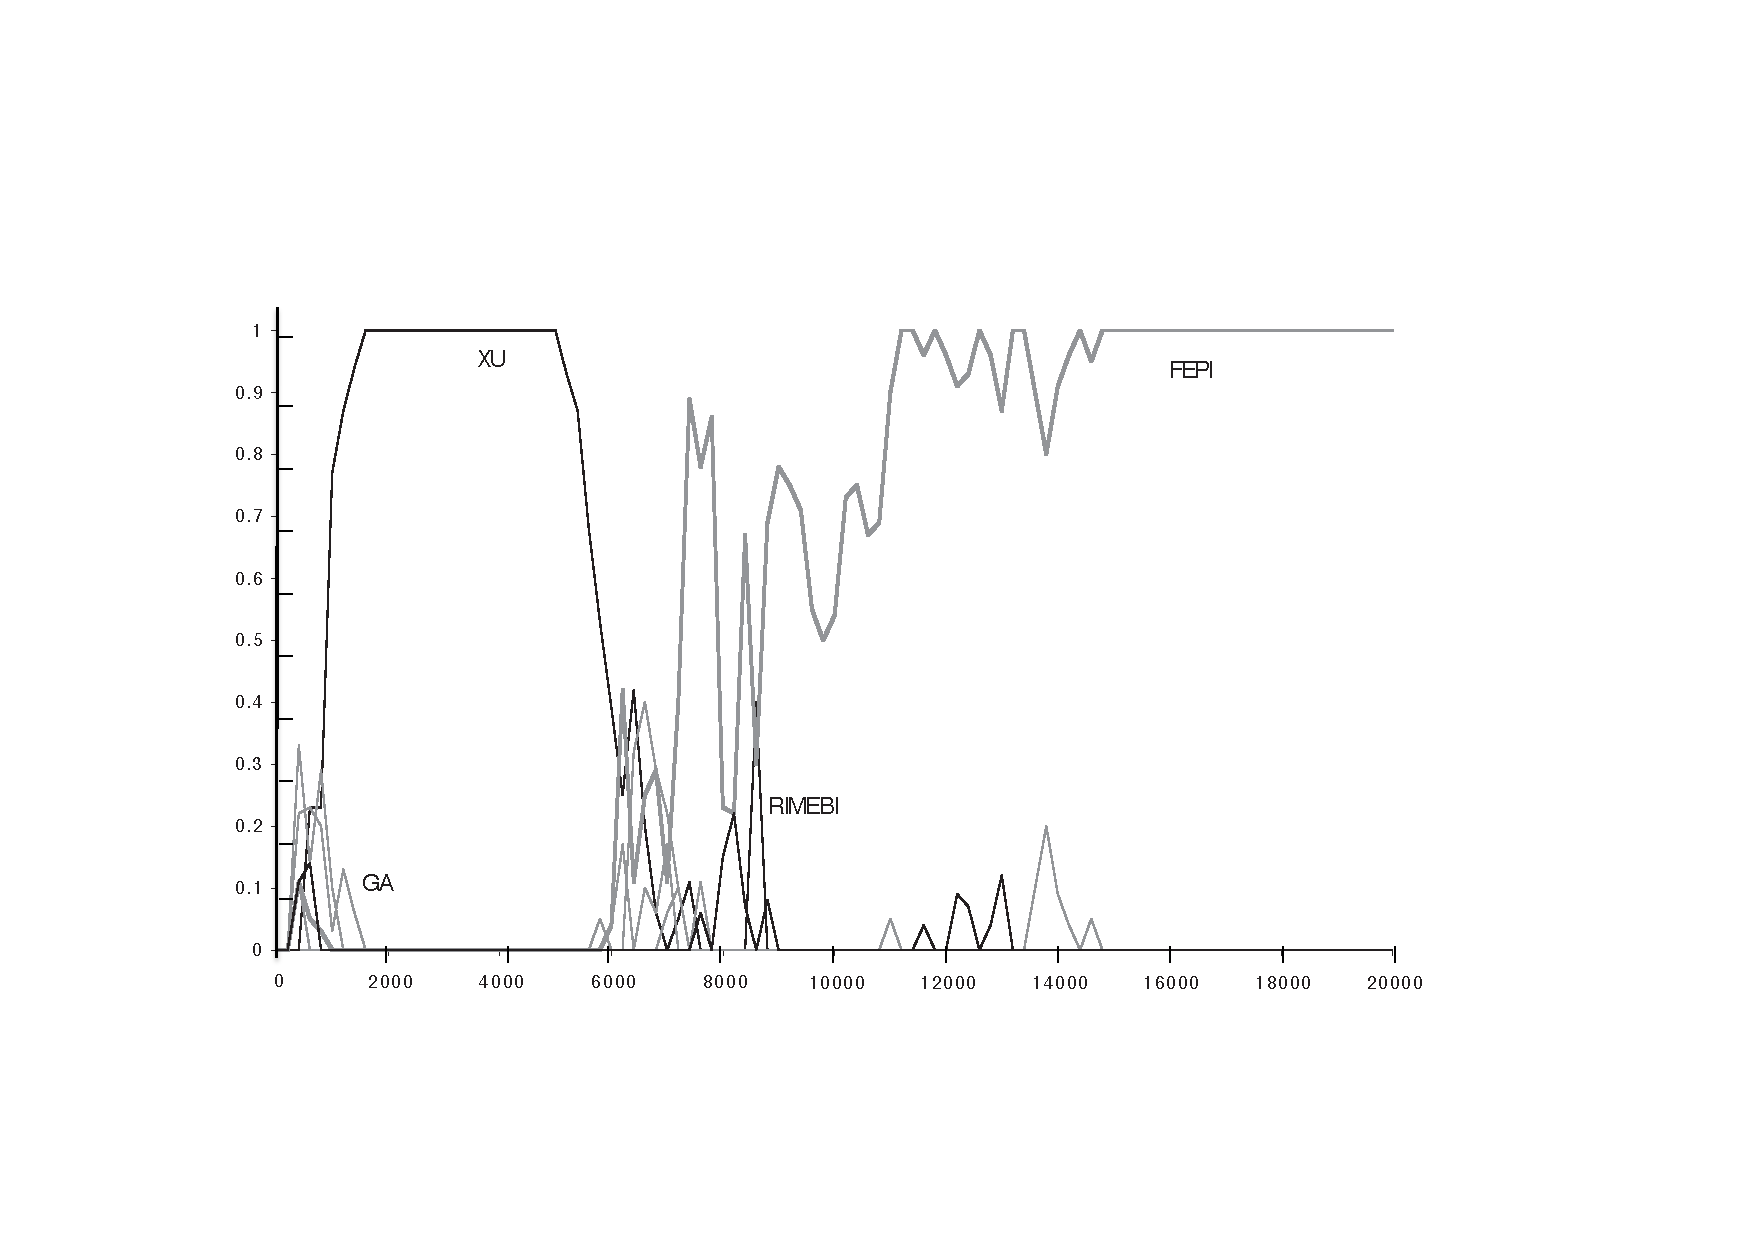
\includegraphics[width=.80\textwidth]{chap2/figs/competition-1}}
\caption{\label{competition1} 
The graph shows the competition between different forms for
expressing one meaning in a population of 20 agents. The graph plots 
the frequency of each form in the population, more precisely the percentage
of agents that prefer a particular word. A complex dynamic
process unfolds with periods where one word (first ``xu'' and then ``fepi'') dominates.} 
\end{figure}

\subsection{Disambiguation}

Another difficulty which I did not deal with when discussing game 25 above,
is that the hearer may conceptualise
the scene differently from the speaker. For example, 
the triangular object is not only located at the lower half
of the scene and the rectangle at the upper half, 
but it is also to the left, i.e. with $HPOS < 0.5$, whereas
the rectangle is to the right. It follows that the 
hearer could just as well have hypothesised that ``lu'' means [HPOS 0.0-0.5] (left)
and not [VPOS 0.0-0.5] (lower). 

Is this bad? It depends on the situations being encountered
in the future. When the game is played again for the
same scene with {\bfshape a1} saying ``lu'' to mean [VPOS 0.0-0.5], and 
{\bfshape a2} interpreting ``lu'' as [HPOS 0.0-0.5], the game would succeed! 
Communicative success is achieved whenever the 
hearer recovers the referent chosen by the 
speaker; it is not required that they 
use exactly the same meaning. In fact, the hearer can never know
for sure what meaning was initially conceptualised by the speaker and 
neither can the speaker know which meaning was understood 
by the hearer because they cannot look inside each
other's head. The meaning can be quite different, 
as we have just seen, as long as it is compatible. 

Even more remarkably, if a topic which is at the lower
portion of the scene, is always 
on the left side and vice-versa, there would always be 
success despite the different meanings of ``lu'', 
and the players would never discover
that each means something else by ``lu''. 

Similar situations arise in human natural language communication
as well, particularly for words
which are not stabilised yet or whose interpretation 
depends strongly on the non-verbal information provided
by the context. They also arise when the speaker or hearer
have different sensory modalities or sensibilities. 
For example, a colour-blind person (unable to 
make the distinction between red and green) will recognise
the red traffic light by its position. For that person, 
``stop for the red light'' does not mean stop for 
the light that has the colour red but stop when the 
upper-most light is lit. 

These examples show clearly that shared language and meaning 
arise from the efforts of agents to co-ordinate their
conceptualisations and lexicalisations with respect 
to the environments they encounter and the games they play, 
but that these co-ordinations cannot be perfect nor totally 
uniform because the agents have limited rationality. 
In general, we can {\itshape not} assume that different agents
have exactly the same 
conceptualisation of reality and that they mean the same thing by 
the same words. As we will see in later experiments, the
Talking Heads hardly agree on the meaning of a word, particularly 
in the early phases of language development, but they 
nevertheless manage to have a surprisingly high communicative success
rate. There is no guarantee that a particular 
form maps onto the same meaning, even in the same language community.
Despite these shaky foundations, communication is generally 
successful because there is sufficient coherence among the members of 
a community and sufficient constraints from the context. 


\begin{figure}[htbp]
  \centerline{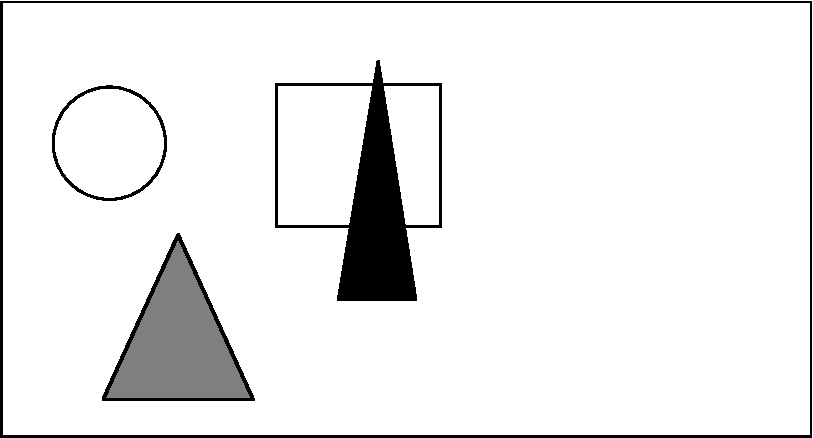
\includegraphics[width=.50\textwidth]{chap2/figs/scene1-2}}
\caption{\label{scene1-2} A second scene which 
can be used to disambiguate ``lu''.}
\end{figure}
Consider now another scene (\figref{scene1-2}). The speaker
is again {\bfshape a1} and categorizes the bottom triangle as 
[VPOS 0.0-0.5]$_{\mathbf  a1}$, meaning
the object at the lower half of the scene. Assuming that the
hearer {\bfshape a2} has associated ``lu'' with [HPOS 0.0-0.5]$_{\mathbf  a2}$, he
would interpret ``lu'' as [HPOS 0.0-0.5]$_{\mathbf  a2}$ (to the left). But this 
does not yield a single 
referent and therefore the game fails. 
This failure is an opportunity for the hearer to repair his 
hypotheses about the possible meanings of ``lu''.
When he conceptualises the scene himself, 
he finds that [VPOS 0.0-0.5]$_{\mathbf  a2}$ distinguishes the triangle
from the circle. A new association between 
"lu'' and [VPOS 0.0-0.5]$_{\mathbf  a2}$ is stored. The old association
is not removed but enters in competition with the new
one, and gradually one meaning will come to dominate
by the winner-take-all mechanism discussed earlier on. 

The commentator reports this kind of interaction as follows: 
\begin{verbatim}
Game 137.
 a1 is the speaker. a2 is the hearer. 
 a1 segments the context into 4 objects
 a1 categorizes the topic as [VPOS 0.0-0.5]
 a1 says:  "lu"
 a2 interprets "lu" as [HPOS 0.0-0.5]
 There is more than one such object
 a2 says: "lu?"
 a1 points to the topic
 a2 categorizes the topic as [VPOS 0.0-0.5]
 a2 stores "lu" as [VPOS 0.0-0.5]
\end{verbatim}

Through such disambiguating situations, meanings of words
get clarified and the lexicons of the agents
become more similar. Note that the 
dominating meaning of ``lu'' can still go in 
two directions. For example, {\bfshape a2}
could have used ``lu'' with {\bfshape a1} 
in a situation where its only possible meaning 
is [HPOS 0.0-0.5] (left). Then {\bfshape a1}, now playing the role
of hearer, would have stored the association between
``lu'' and [HPOS 0.0-0.5]. If this happened often 
enough [HPOS 0.0-0.5] (left) might
have become the dominant meaning of ``lu'', instead of 
[VPOS 0.0-0.5] (lower). This shows clearly that the 
evolution of language will never be predictable. At a critical 
bifurcation, small preferential differences between 
the agents or the chance occurrence of certain situations
may tilt the competition in one direction or the other.\footnote{
This high sensitivity to initial conditions is 
one of the characteristics of a chaotic dynamic
system \cite{Lorenz:1993}.
Indeed, as I will explore in more detail later, 
evolving languages have all the characteristics
of complex adaptive systems, including the 
potential for punctuated equilibria.}
There is no right
or wrong solution in the language game and no one has
any more rights than anyone else. 

\subsection{Same meaning, different referent} 

When agents have the same meaning for the same
form, it is likely that they
pick out the same referent from the context. When agents
have a different meaning for the same form, it is less 
likely although it may still happen that they pick 
out the same referent, as we have seen. But there 
is an even more problematic situation: When agents have the 
same meaning for the same form but nevertheless pick out 
different referents! 

For example, suppose that two Talking Heads have developed the 
concept of [LEFT] and [RIGHT] with respect to their own position 
in front of the scene. In terms of the sensory 
channels we have been using, anything to the left of their field  
of vision ($0.0 \le HPOS < 0.5$) is categorized as
left, i.e. [HPOS 0.0 0.5], and everything right  
($0.5 < HPOS \le 1.0$) is categorized as right, 
i.e. [HPOS 0.0 0.5]. But because the
agents stand next to each other and have therefore 
slightly different positions with respect to the 
scene in front of them, there is an area which will 
be categorized as right for one head and left for the other (\figref{2:left-right})

\begin{figure}[htbp]
  \centerline{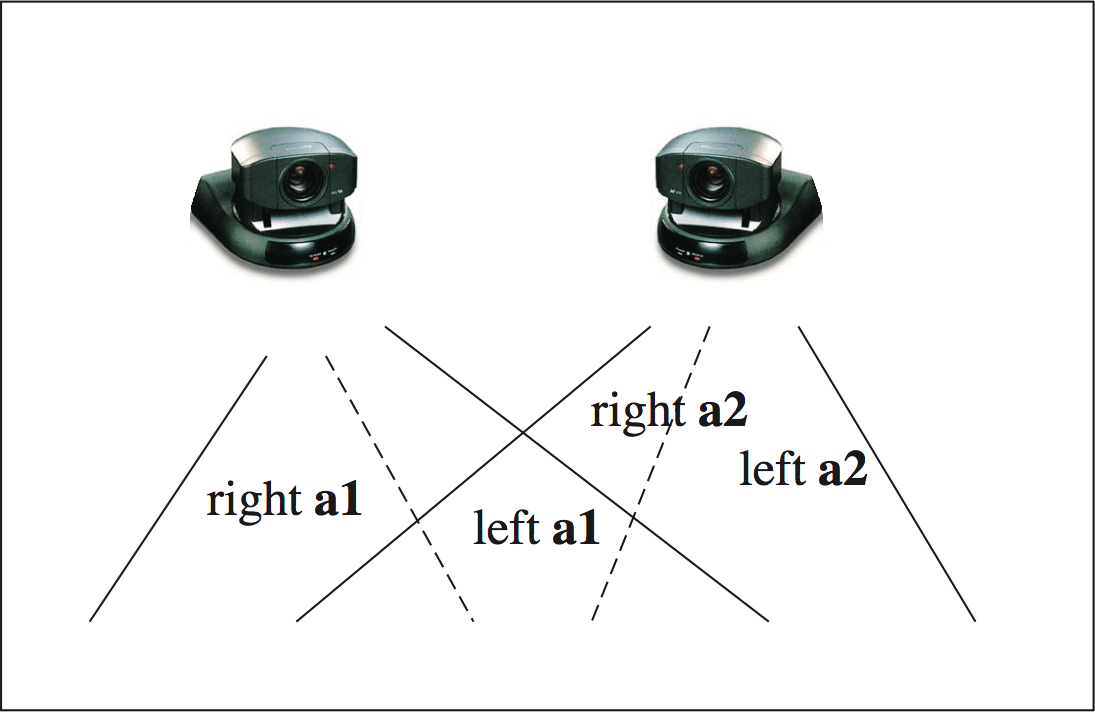
\includegraphics[width=.65\textwidth]{chap2/figs/left-right}}
\caption{\label{2:left-right} Two talking heads are shown {\bfshape a1} and 
{\bfshape a2} each seeing the scene from a slightly different viewpoint.}
\end{figure}
When this occurs in real dialogs, the form-meaning 
pairs lexicalising the distinctions left and right destabilise,
because sometimes it gets positive feedback as 
it succeeds in the game, and at other times it 
gets negative feedback. 
This is one of the reasons why human categories are often 
relative and scaled with respect to a context.
For example, we say ``the triangle to the left of the square'', in 
other words left with respect to the square, to avoid the uncertainty
inherent in the absolute use of ``left''. Humans scale the size 
of objects with respect to the scene, so that small 
objects are small compared to the others in the scene 
and not small in an absolute sense. 

\subsection{Situated grounded semantics}

These various examples, and I am clearly only \is{situated grounded semantics}
scratching the surface, already illustrate the major thrust of the 
approach explored in more detail in the remainder of this book. 
There are dynamic processes at two levels. (1) There is 
the evolution of a lexicon in a single agent: new words are
invented or adopted from another agent and the
scores of form-meaning pairs in the lexicon
go up and down depending on success or
failure in the game. At any point in time, an agent 
will have a preferred form to express a particular meaning, 
but he has also stored the alternative words floating around in the 
population, and his preference will change depending on feedback
in further language games. (2) There is also lexicon evolution at 
the level of the group. A coherent global lexicon emerges because
the lexicons of the individual agents become more and more 
similar. This is due to the positive feedback loop between
the outcome of using
a certain form-meaning pair and the probability that
this pair will be used again in the future. 
The group lexicon will however seldom be exactly uniform because
new meanings constantly pop up and agents may arrive from 
other language communities, bringing in new words. 
I will study this two level dynamic process in much more detail 
in chapter 7. It explains many of the mysteries of
language, for example why there is ambiguity. 

The `semantic theory' required to make the 
Talking Heads experiment work is very different from 
the classical textbook approaches to the subject, which
tend to assume that categories can be defined in the 
abstract, independent of their context of use. Grounded
conceptualisation and interpretation processes are necessarily 
strongly situated and context-dependent. Whether ``blue 
triangle'' is going to be effective in picking out the 
intended topic depends on what else is in
the scene. If all other objects in the 
context are also blue triangles, the game will fail. If there
is only one triangle, it was not really necessary to say that 
it is blue. This situatedness and context-dependence, together with 
the non-verbal hints given by the speaker, are crucial 
keys for restricting the 
possible meanings of a form 
and they therefore help the hearer disambiguate 
utterances or figure out the meaning of an unknown form. But situatedness 
and context-dependence are also major
sources of difficulty, because the same categories may
refer to different things for different agents in different
contexts. Even if both agents agree that a particular form 
names a certain category, 
they may still fail in the game if the category picks
out a different referent, for example because they see 
the context from a slightly different vantage point. 

Another major difference with classical theories of 
meaning and reference is 
that the repertoire of meanings and form-meaning pairs is open-ended
and subject to change at any time. Logicians would say that the 
truth conditions of the forms are non-monotonic. \is{non-monotonicity}
Non-monotonicity is unavoidable in the case of grounded 
situated agents with limited rationality.\footnote{
Examples of these processes are described in: 
\cite{Bybee:1994}, \cite{Traugott:1991}.
For attempts to explain these ``grammaticalization'' 
processes in terms of general cognitive operations, see: 
\cite{Heine:1997}.}
Agents should always be allowed to 
introduce new forms or recruit existing forms to express new
meanings, simply because the set of meanings must expand
to cope with novel contexts and new communicative
situations. After enough interactions among the 
members of the same group in a relatively stable 
environment, we expect there to be
a stable set of conventionalised form-meaning 
relations, but it cannot be
expected that everything anyone ever wants to say is
already conventionalised, and so there will always
be turbulence at the fringes. The idea that the lexicon
and the syntax of a language are static
entities is completely false. Both are in constant flux.
Non-monotonicity is consequently one of the big 
topics in logic-based approaches to artificial intelligence.

A theory of language must try 
to capture the strategies by which language users shape and 
reshape their language and by which some solutions may become 
conventionalised and spread in the rest of the population, 
rather than focus on describing the end results of 
this process. This open-ended adaptive character of 
language systems is explored extensively in chapter 7. 

This section probably raised many questions in the 
mind of the critical reader: Will the agents really 
reach a sufficiently similar lexicon to have successful 
communication, despite the fact that no one has a 
complete overview nor controls globally what the others
can say? Are the unclear situations, i.e. those
where more than one possible meaning is possible, not 
going to destabilise existing lexicons? Will all this 
scale up both for the size of the agent set and for 
the size of the meaning set? Is a new, virgin agent 
going to be able to catch up with a lexicon already 
existing in a population? What happens when two 
populations each with their own entrenched lexicon meet? 
These are exactly the kinds of questions that I will 
address later. They can all be posed in a precise 
way within the context of the Talking Heads experiment.

\section{The origins of grammar}

The self-organisation of a shared lexicon in a population
of agents already represents a formidable challenge.
We need to find models that work in principle {\itshape and} 
we have to make them operational on physically 
instantiated autonomous robots. 
But many linguists would claim that this does not yet 
represent true language, they would want to see the 
emergence of a genuine syntax. How that might
happen is one of the ultimate remaining scientific
mysteries of our time but let me sketch a possible approach. 

Basically, I hypothesise that the agents must 
first of all have the capability to generate much 
more complex semantic and pragmatic strategies for conceptualising
reality or applying a conceptualisation to retrieve 
a referent.

For example, a phrase like ``the two red
triangles to the left of the smallest green square'' requires
the following strategy: 
\begin{enumerate}
\item The agent filters the set of possible objects in 
the scene to retain only the squares. 
\item He further filters the resulting set to retain only 
the green ones. 
\item He orders the remaining green squares based on 
size and then picks out the smallest one. 
\item Then he orders the objects in the scene based on 
their horizontal position (HPOS) and retains only those
whose position is to the left of the smallest green square. 
\item From the remaining set he filters out the triangles, 
and from this set those with a red colour. 
\item This final set should contain only two members
and they constitute the referents of the original phrase. 
\end{enumerate}
Our research has already lead to  
mechanisms whereby agents can autonomously generate such
semantic strategies using processes that compose
primitive strategies into complex ones. The
strategies compete for use in language games. 
New strategies form when needed by the environment or 
the agent's interactions and those that do not work or 
are irrelevant get pruned. The mechanisms for generating 
and selecting such semantic strategies are not unique
to language. The invention and use of tools or the 
planning of a series of actions and the retrieval 
and use of ready-made plans requires exactly the 
same sorts of capabilities. 

The spontaneous generation of repertoires of complex 
semantic strategies already explains some characteristics 
that are reflected in full-fledged languages: 
There is hierarchical structure, because one strategy 
may call upon another strategy to achieve a subgoal, 
and a strategy may potentially call upon itself thus introducing 
recursivity. There is also a functional specialisation
of categories. They are now sometimes used for filtering
the members of a set, sometimes for ordering them, sometimes
for modifying another category before it is used for 
filtering, and so on. Hierarchical structuring, recursivity
and functional specialisation therefore do not have to 
originate in language. The fact that we see them in 
language structure is a reflection of the generic 
hierarchical and functional nature 
of semantic strategies.\footnote{
The fact that languages change is, of course, 
well-known in linguistics even though it is less a focal 
research topic than used to be in the 19th century. 
See: \cite{McMahon:1994} for a brief introduction into the 
subject. Language change has many of the characteristics
of biological change but it takes place in cultural 
as opposed to biological time. See: \cite{Labov:1994}}. 

Second, my hypothesis is that the need for communicating 
more and more complex semantic strategies and the 
conceptual structures they use, has pushed language 
users to start using more and more complex form characteristics, 
starting with word order but also intonation, stress 
patterns, function words, morphological variations of words, 
etc. Here another aspect comes into 
play: the ability to recognise forms and structures, 
which we also need to recognise structured objects in 
scenes for example, and the ability to assemble a 
structure satisfying a set of constraints. The collective
dynamics which are responsible for the propagation and the spontaneous 
self-organisation of coherence in lexicons should also apply  
here. Grammars can be seen as ecologies, where
form-meaning pairs compete in the population. New 
syntactic and semantic categories, new constructions and 
new uses of grammatical conventions are continuously created,
and existing ones may destabilise and become
in disuse.\footnote{
The semantic strategies are similar to the 
cognitive processes that have been studied extensively 
in cognitive grammar \cite{Langacker:1987}. Formal versions
of some of these processes have been formulated as 
part of Montague grammar \cite{Montague:1974}. In 
computational linguistics research, various 
attempts have been made to formalise conceptualisation
and meaning application strategies. \cite{Gazdar:1989}}

Each language user employs his own ideolect which is 
as well as possible co-ordinated with that of other
language users but there is never complete similarity 
and never absolute stability.  
This explains perhaps why linguists have such a hard
time to pin down ``the'' language of a community. As soon 
as someone speaks, language changes. 

According to this theory, natural language structure is
not the consequence of an 
autonomous innate language device which evolved 
by a genetic mutation or series of mutations. Instead 
cognitive mechanisms and structures already in place have been 
marshalled to get a language system off the ground, even though 
once language became essential for the rapid incorporation
of new individuals and the general organisation of 
activities in human populations, it must have started
to recruit vast amounts of brain capacity and stimulated 
other cognitive faculties, such as categorisation,
episodic memory or problem solving, to become in turn 
much more complex and versatile.\footnote{
There has been an ongoing nature versus nurture debate 
with respect to the origins and acquisition of language. 
The different issues in this debate are already well
illustrated in \cite{Piattelli:1980}.} 

Before the problem of syntax can 
be tackled seriously, we must have a solid foundation showing 
how agents are capable of autonomously acquiring individual words
or combinations of words without syntax. This is the subject of the
remainder of the present volume.

\section{Conclusions}

The Talking Heads experiment examines with what kinds
of mechanisms physically embodied autonomous agents 
might be capable of bootstrapping an ontology, a lexicon, 
and a syntax. The Talking Heads are situated embodied
agents. This 
allows them to build up and co-ordinate language and meaning 
in tight interaction with a shared physical environment
as perceived through their cameras. 
The Talking Heads are social agents, members of a
language community. The collective
dynamics of the community is a crucial ingredient to understanding
how successful communications of a similar complexity as
human natural language communications might have 
originated and how the underlying system can 
be maintained from one generation to the next. 

This chapter has described the main hardware 
and software components of the agents and briefly sketched
their internal architecture. The operation and effect
of this architecture have been 
illustrated with some example games. The remaining chapters explore the 
various aspects of the agent's capacities in much more detail. 
First I will break the global task down into different subtasks, 
as suggested by the semiotic square. We will start by looking how agents 
may establish the relation between a real world object and 
a segmented image (chapter 3). Then we study how they 
relate a segmented image to its conceptualisation (chapter 4). 
Third, we study how a conceptualisation can be related to 
an utterance (chapter 5). In chapter 6 and 7 we couple these
various components and study the lexical and ontological 
dynamic processes that result. 

%\end{document}


%\documentclass{../_combined/fcg-book}
\chapter{Perception}
Our minds deceive us. Intuitively we feel we see very clearly and 
unambiguously the objects in our environment and are able 
to categorize objects or actions unequivocally in terms of 
perceptually grounded distinctions. For example, when 
I look out of the office window at the inner 
courtyard garden, I can clearly see the plants, trees
and birds, as well as the walls, windows, and doors of 
the surrounding buildings. I can categorize their 
colours, sizes, and shapes and determine whether the 
leaves of the trees are moving with the wind. Because of 
this categorisation I can describe to another person what 
I see. 

A categorisation and conceptualisation
of reality is fundamentally based on sensors which output 
signals that directly 
reflect, in an analog and partially unreliable way, physical
properties of the environment. For visual perception, 
human beings have photosensors in the eye which correlate 
with the amount of light, i.e. the amount of 
photons, falling on the sensor. The more photons, the stronger
the sensor signal. But, a photosensor, or a matrix of 
such sensors as in the human
retina, does not tell anything more than what the light
intensity is at a tiny spot of the image captured
by the eye. There is no obvious straightforward
procedure that groups the spots 
into coherent patches.
When you implement and tries out different segmentation procedures
on real world images, you quickly find that each procedure
generates a multitude of possibilities instead of a clear 
segmentation. Even if
coherent segments are detected, there is the problem of what 
features of the scene are going to be used for further
conceptualisation. A very large, open-ended
set of possible feature detectors can be
imagined. The quality and reliability of their
output depends on the scene being processed, and is in any 
case strongly context-dependent. 

So we find that the world does not present itself neatly segmented, 
processed, and categorized. There is an enormous 
gap between the symbolic world of objects and categories
and the subsymbolic world of analog sensing. 
The brain somehow performs a vast amount of processing
to fill this gap, without us being in the least aware of it. 
This processing takes place in parallel. Many different
segmentation procedures and feature detectors 
operate concurrently on streams of consecutive images, 
generating hypotheses that become stronger if they are
confirmed by additional evidence, or weaker if 
they do not fit into a larger picture. We are only 
aware of the final result and therefore have no 
intuition of what is really going on, except
in rare and pathological circumstances. 
Rather than viewing perception as a straight-forward step-by-step
transformation of the raw sensory data into a segmented
picture, it is better to think of the whole process
as a boiling soup with thousands of hypotheses taking
shape, some of them floating like bubbles up to the surface. Constraints
and expectations flow down from the top so that the maximum 
amount of available information is used to construct the 
coherent segmented picture of reality we consciously experience. 

The objective of this chapter is to examine this 
process in sufficient detail to move forward with the main
topic of our investigations, namely language and meaning. My 
aim is not to delve into the full complexity of the 
visual system, because this would lead us too far 
astray of the main topic, but to have a sufficiently 
rich source of features so that conceptualisation and 
language communication can be studied. 

\section{What sensors sense}

Sensors and actuators are the interfaces between the physical
world and the internal world. \is{sensors} \is{actuators} They are 
dedicated hard-wired components and grow in biological 
systems strongly influenced by genetics and environmental inputs.\footnote{Possible 
biological implementations of the various 
sensors and sensory processes discussed in this chapter 
can be found in \cite{Churchland:1992}. The 
nature and neurophysiological implementation of visual
processes are discussed in detail in \cite{Zeki:1993}.}

A sensor transduces external physical 
states into internal states. For example, a touch sensor, of which 
there are hundreds of thousands all over the human body, 
transduces mechanical energy into neural signals. Other sensors
respond to the intensity of certain sectors of the wave spectrum. 
Ears respond to audible waves. Photoreceptors in the eye
respond to visible light waves. 
The body also has a large number of
biochemical sensors responsive to internal 
chemical states so that we can feel the hunger in our stomach for example. 
In addition to sensors, bodies carry 
actuators, which transduce internal states into mechanical 
energy and thus make it possible to perform actions in 
the world. Actuators receive continuous signal streams and modulate
their activity based on these signals. 

\subsection{Artificial Sensors and Actuators}

Analogs of biological sensors can be artificially recreated to give
robots sensory capabilities. Something similar to 
a touch sensor can be created using a contact switch 
that passes current when closed. A microphone has 
a functionality similar to the ear. 
A digital camera can be used to recreate the functionality of an eye; 
it records the light intensity of millions of small rectangles of 
the image, known as pixels, just like the retina. The set of 
all pixels is usually called an image map. Digital
colour cameras provide three information elements for 
every pixel: the amount of red, 
green and blue of each pixel (RGB). We 
can build sonar sensors responding
to low frequency waves, just like the ones bats use 
for navigation, or infrared sensors which are useful 
for obstacle avoidance because 
the amount of infrared light emitted and captured back
by the sensor correlates with distance to objects. 

A sensor should never be seen as measuring accurately 
an abstract property of reality. For example, an infrared sensor 
does not measure the distance to an obstacle. The infrared
reflection depends not only on distance but also
on the reflection properties 
of the object and on the amount of background infrared 
in the environment, thus distance must be inferred and projected onto
reality. Similarly, the colour receptors do not really measure
colour. They respond to reflections within segments of the wavelength spectrum 
but this reflection is again determined by many factors: how much and what kind of 
light falls on the object, and how the object reflects the light depending which varies 
with the position of the object. So colour is again a more abstract notion that needs to be 
reconstructed and projected on the image based on complex processing. 

The Talking Heads use vision as the main source of
sensory information because most of the perceptually 
grounded concepts used in language derive from visual
sensing. The only actuator (apart from the speech 
synthesiser which I will not discuss in detail) 
is a pan/tilt motor for turning the head up and down 
or left and right. 

\subsection{Natural sensing}

It is technically possible to build all sorts of 
sensors and actuators that have little to do with
human capabilities. But clearly, human-like categories and languages 
that are similar to human categories and languages will only 
emerge if the sensors and actuators are at least to some degree similar to those
of humans. This is not always technologically 
possible and when it is, it often 
requires non-trivial transformations of artificial 
sensor data. The Talking Heads use digital cameras 
as their main sensory source. These cameras give output 
in RGB (red, green, blue intensities) because this 
is the standard in current computer 
technology. But human vision operates
on four quite different channels: the two chromatic 
opponent channels which provide a value on the 
yellow-blue and red-green dimensions, an achromatic 
channel which holds the brightness or light 
intensity, and a saturation channel which reflects the 
degree of saturation or purity of a colour. These 
channels can be reconstructed from RGB by a complex 
transformation.\footnote{
There is a vast literature on colour perception from 
different points of view (physics, psychology, 
neurophysiology, linguistics). A representative sample 
is contained in \cite{Byrne:1997}. 
In some of the experiments described later, the RGB values
are converted to the CIE XYZ colour coding and from 
that to the opponent channels. 
These algorithms have been implemented by Michael
Pollitis. See: \cite{Kaiser:1996}. 
}

\subsection{Behaviors}

Although language requires that the image is 
segmented and categorized, a lot can already
be done with raw or lightly processed sensory data
by dynamically coupling them to signals 
controlling the actuators. The neural abilities
of many simple animals probably do not get much further
than this and it already has turned
out to be a good way to construct the basic behavioral
layers of robots that have to operate autonomously 
in a real-world environment in real time. 

For example, suppose we want a robot of the sort seen 
in \figref{f:plate3} to move towards a light source. As originally 
suggested by the cybernetician Valentino Braitenberg,
\cite{Braitenberg:1984}. 
we can do this by mounting two simple light sensors 
to the left and right of the body and by implementing a 
direct dynamical coupling between the output of the light
sensors and the motors. The coupling is such that when
the sensed left light is stronger than the sensed right
light, the motor attached
to the left wheel is slightly decreased and the right
motor slightly increased, so that the robot veers to the left. 
When the right light is stronger, the right motor is 
increased and the left motor decreased, so that the 
robot veers to the right. When these two dynamical 
couplings are put in place together with a
forward movement, a zig-zag behavior emerges which
brings the robot to the light source. \is{behaviors}

Basic behaviors can be put together to form 
more complex behaviors.\footnote{A representative sample of experiments in this 
direction is reported in: \cite{Steels:1996}. See 
also: \cite{Arkin:1998}.}
\figref{phototaxis} 
shows a recording of the internal states of the robot
in \figref{f:plate3} as it is performing 
phototaxis towards a light source, using two simple
light sensors, and touch-based obstacle avoidance
behavior.  When the robot strikes the box housing 
the light, it moves back in a kind of reflex behavior
triggered by the touch sensors mounted at the front. 
The $LeftLight$ and 
$RightLight$ sensory channels and the $LeftMotorSpeed$ 
and $RightMotorSpeed$ are shown 
in \figref{phototaxis}. When the robot strikes
the obstacle housing the light, its left and right
motor is pulled down to a negative value so that 
it moves backwards. Then the robot zig-zags to the 
light source until it hits the obstacle again. 
\begin{figure}[htbp]
  \centerline{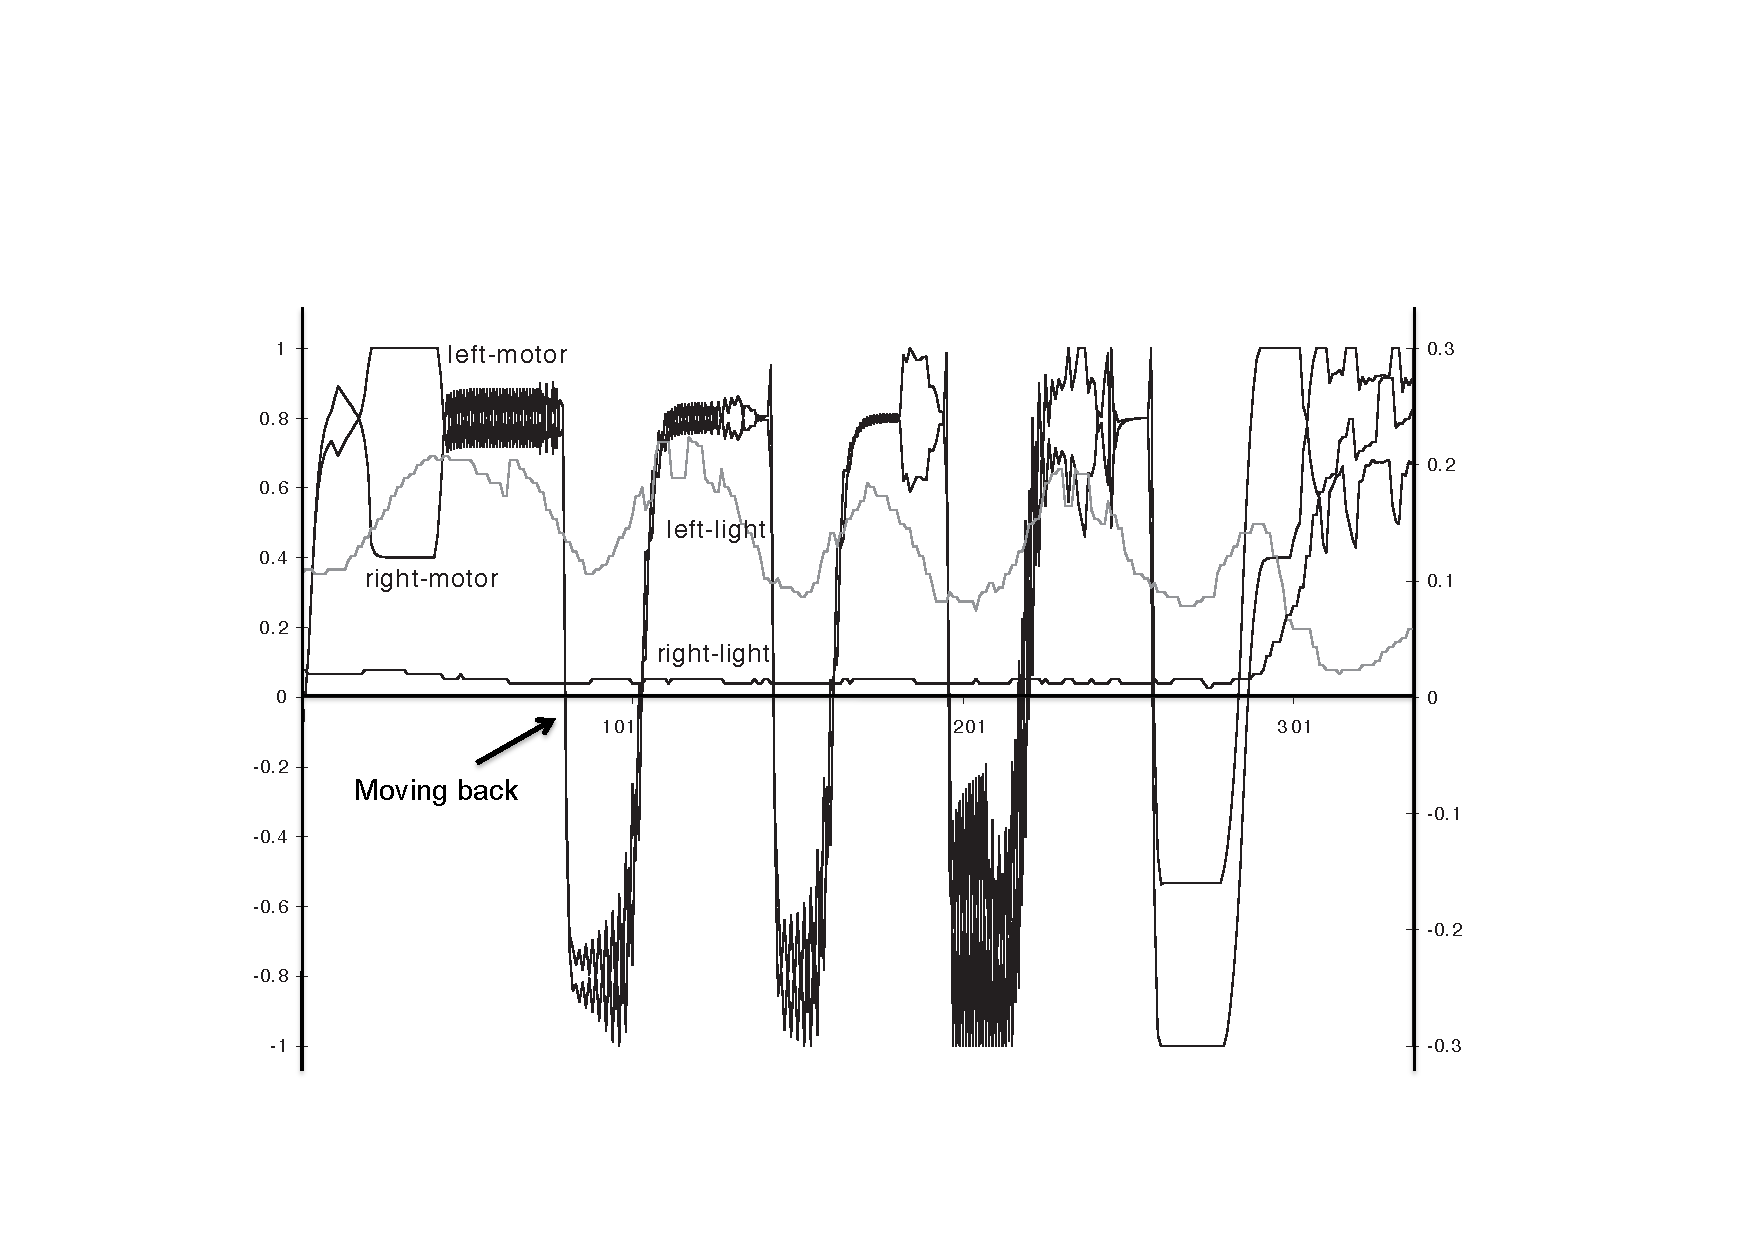
\includegraphics[width=.85\textwidth]{chap3/figs/phototaxis}}
\caption{\label{phototaxis} 
Internal states of a robot's sensory and actuator channels on 
the y-axis and time in periods of 1/40 second on the x-axis.
The robot pushes against a box holding a light source.}
\end{figure}

These channel recordings illustrate clearly that sensor or actuator
data is continuous in time and 
rapidly fluctuates in response to changes in the environment or the
behavior of the agents. Coupling sensory data to actuators
is effective for quick reaction
without the need for higher level processing. If 
an obstacle is rapidly approaching, it is important to get out 
of the way rather than trying to figure out what kind of 
obstacle it is. The observed behavior is very complex, even though
the underlying dynamical systems are relatively 
simple; the complexity is due to the complexity of the 
real world with which the robot is interacting. 

Similar behavior systems and networks have
been experimented with 
for more complex tasks and it is actually the way that 
the Mars rover discussed in the introductory chapter works.\footnote{At 
the risk of simplifying, we can say that the early 
work in cybernetics (such as that of Braitenberg
referenced above) has focused on this subsymbolic layer
and that `Artificial Intelligence' as a research field
emerging in the late fifties has focused on the 
symbolic layer. Some researchers involved in a bottom up 
approach to Artificial Intelligence strongly refocused
on the subsymbolic layer. One of the most
vocal advocates of this position is \cite{Brooks:1992}.
Obviously we need the two, 
but bridging the gap is a non-trivial problem, sometimes known 
as the grounding problem. See: \cite{Harnad:1994}. }
However, the gap between the continuous dynamics of sensori-motor
intelligence and cognition remains unbridged. 
It is possible for {\it us} to see 
structure in the data but this structure is not perceived
nor used for control by the robot itself. 
The robot does not segment nor categorize
reality. It does not `know' that it is moving left or right 
and therefore cannot communicate this information to another robot. 
All processing remains at the analog continuous
level. However because it remains at this subsymbolic level, it is doubtful
whether we can ever hope to bootstrap cognitive
intelligence simply by adding more of these dynamical 
systems.\footnote{
\cite{Marr:1982} remains a classical reference outlining
the features that can be extracted, the
principled algorithms for doing it, and possible 
neurophysiological models. These are the main research
topics that still dominate research in vision. See 
\cite{Ullman:1996} for a more recent overview.}
The difference between behavioral intelligence 
and cognitive intelligence resides in an additional 
layer of processing which is no longer continuous and analog 
but discrete and symbolic. How this second symbolic 
layer could be formed but at the same time remain 
grounded in the analog sensori-motor layer is one 
of the main research topics addressed in this book. 

\section{Segmentation} 

The first step that bridges the gap between sensory layers and \is{segmentation}
cognitive processing is segmentation. Segmentation means that 
a sensory data stream is divided into units 
either in space or in time. In the Talking Heads experiment, 
the environment is restricted to
static images only, so that segmentation
amounts to aggregating pixels into spatial patches.

A patch may have an irregular shape which makes it hard to apply 
some classifications without complex processing. Bounding boxes are much 
easier to compute and are already very useful. The bounding box of a segment 
is a rectangle around the contours of a segment (\figref{f:boundbox}).\is{bounding box} 
\begin{figure}[htbp]
  \centerline{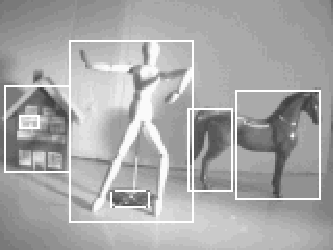
\includegraphics[width=.50\textwidth]{chap3/figs/sslang}}
\label{screenshot}
\caption{\footnotesize Example of a scene captured by the 
camera in \figref{f:plate7}, containing a puppet, a
wooden house, and a horse. Segmentation is based on aggregating grayscale
patches, i.e. areas in the image that are lighter or darker than the 
general background. Bounding boxes have been drawn around the segments. 
Note that there can be bounding boxes within bounding boxes if an object 
forms part of a larger object. 
\label{f:boundbox}}
\end{figure}

It is generally not necessary for segmentation to always yield parts of the images that correspond
to what we would call objects. This is an impossible demand. What counts as 
an object is to some extent task-dependent. 
Segmentation yields information that can be used for 
object identification but should not be equated with it. 
This is well illustrated in \figref{screenshot}. 
Segmentation has been done here by filtering out segments with 
lower or higher average grayscale values compared to the 
average in the scene. The segments that have been obtained
are not necessarily those that we humans identify, because we
use knowledge of the objects involved. This 
shows clearly that higher level constraints play a role 
even at the very first basic visual processing layers. 

\subsection{Feature extraction}

Many methods for segmentation have been reported \is{feature extraction}
in the computer vision literature and all of them are useful even though they 
give slightly different results. Most methods assume 
that additional low level processing is first performed 
on the image map to detect small-scale structures, such as: 
\begin{itemize}
\item Edges, which are possible boundaries between two 
surfaces. Edges can be aggregated in line segments. 
\item Junctions, which are regions where lines come 
together. 
\item Patches, which are regions where the colour or
the grayscale values are relatively constant. 
\item Textures, which are small-scale regular surface 
markings, for example blobs. 
\item Optical flow, which are vectors indicating the 
direction and velocity of moving brightness patterns. 
\item Distance from the observer, computed by
matching two image maps from binocular vision. 
\item Shadings, recovered from continuous variations in
brightness. 
\end{itemize}
The recovery of such features is in itself 
a non-trivial topic of research and a huge literature as well as 
many software libraries now exist.

The visual layer of the Talking Heads only extracts 
patches and edges which each leads to one way 
of segmenting the scene. 
Segmenting based on patches attempts to aggregate 
those parts of the image into patches (a process
called region growing) that have more or less the same 
colour. `More or less the same' is of course a relative
notion and larger or smaller segments will be found
depending on the thresholds that are used for 
deciding whether a colour is similar or not. Segments
that are too small are not considered further. 
Region growing starts by comparing for each pixel how similar it is to 
neighboring pixels. Similar pixels
are grouped as a patch. In the next step, each patch
is examined to see whether it can be merged with
a neighboring patch, and so on recursively until 
patches cannot be combined further. Small patches or individual pixels that 
stand on their own are included as part of a larger
patch so that we get sufficiently broad patches. 

Segmentation based on edges starts by first detecting the 
edges themselves, which are colour discontinuities suggesting a boundary
between two surfaces. The edges are then aggregated into lines, and these lines are 
connected to find the contours 
of an object. This method works well for the simple 
objects used in the Talking 
Heads experiment. Things are
no longer so simple when contours are less
clear, for example because they fuse with the background. 
Further complications arise when one object partly obstructs
another object or when a set of lines can ambiguously 
be organised in different configurations (as in visual illusions
like the Necker cube). This illustrates that one 
segmentation method must be balanced with others to offset unclear 
areas or local ambiguities. 
\begin{figure}[htbp]
  \centerline{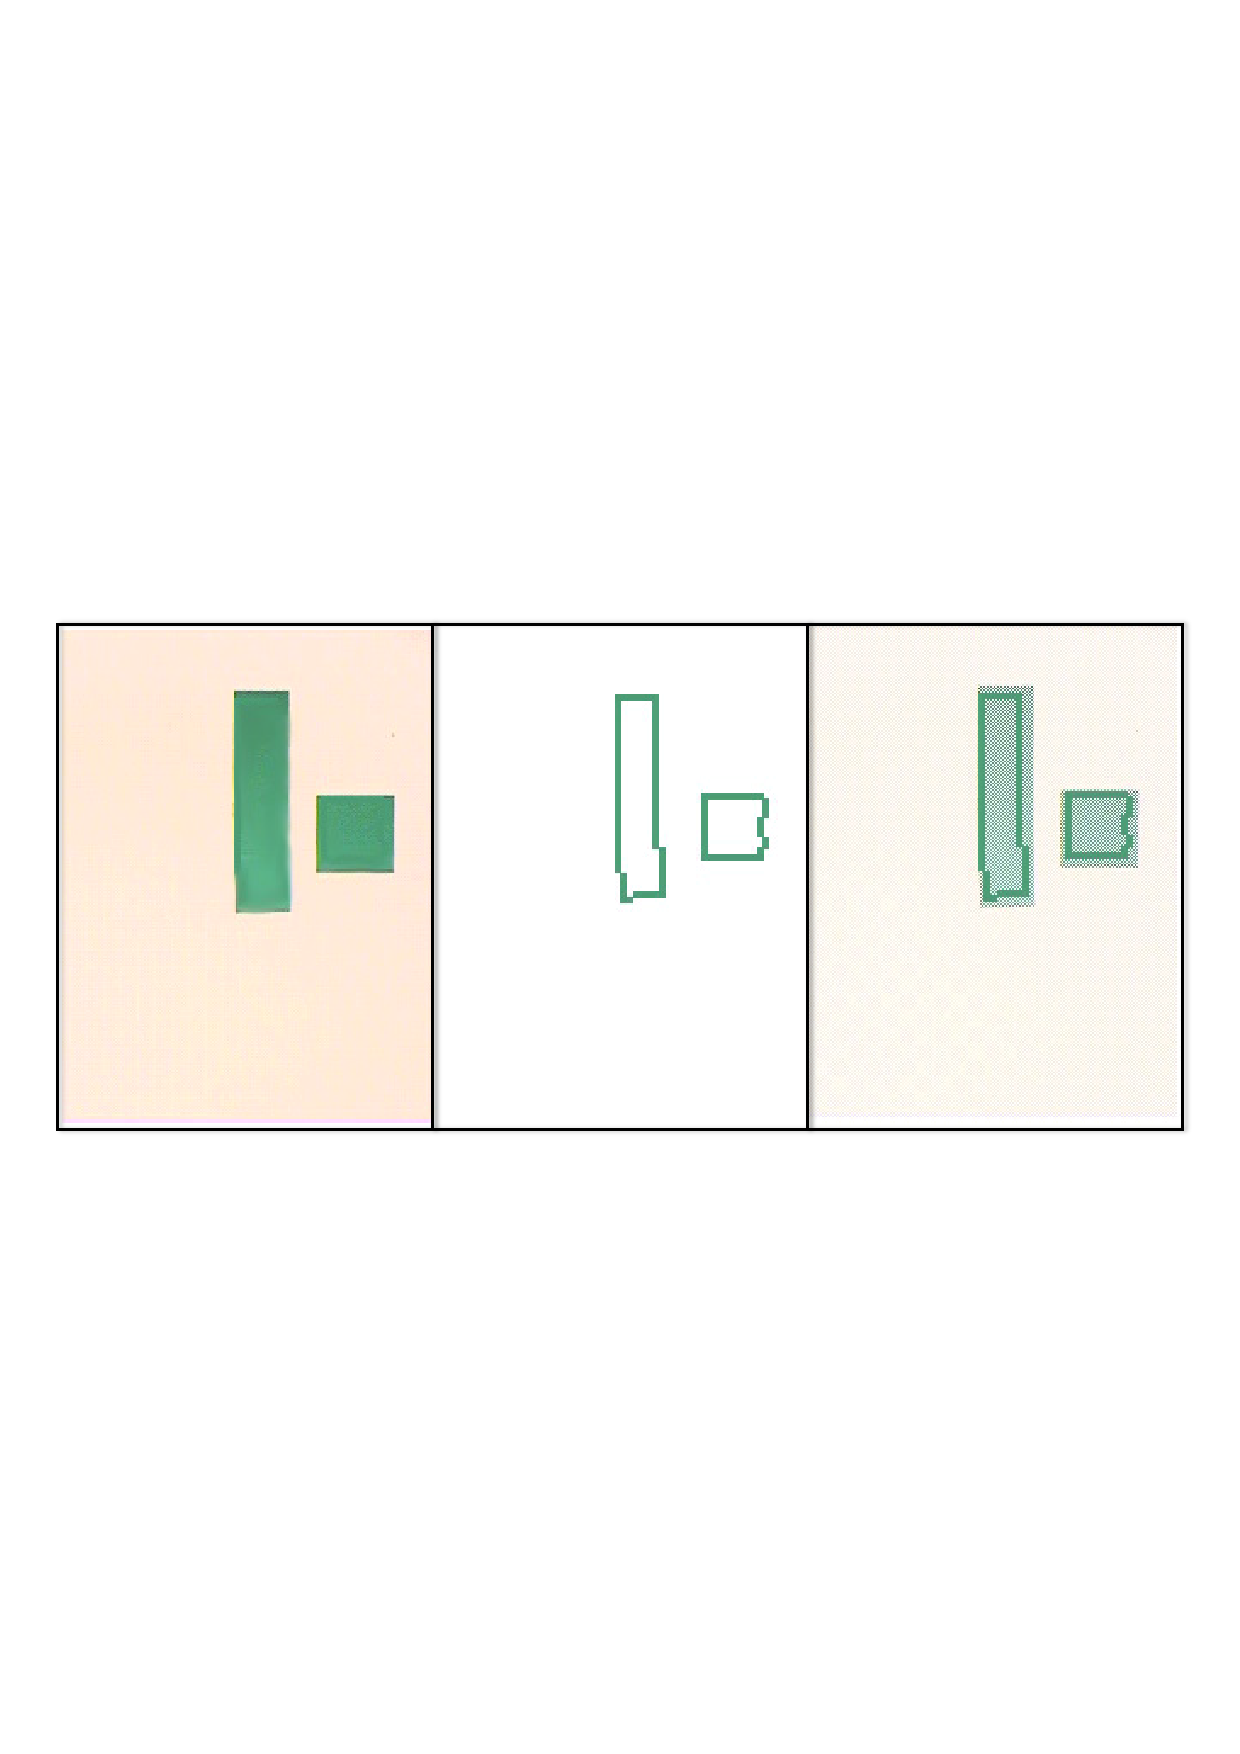
\includegraphics[width=.75\textwidth]{chap3/figs/image1}}
\caption{ Left view shows an image as captured by a Talking
Heads camera. Middle view shows the result of 
segmentation based on edge detection. Right view
shows the integration of segmentation by color
and by edge detection.}
\label{f:plate11}
\end{figure}

The results of applying these two segmentation methods
can be seen in \figref{f:plate11}. 
The top picture shows the image map itself as it is captured by 
a Talking Head camera. The middle image shows the result of 
segmenting based on edge detection. The contours of two 
objects have been found. Note that these contours are not 
straight lines as one might expect. They are obtained by 
connecting together line segments which are themselves 
based on connected edges. The bottom image shows the combination of 
edge detection and segmentation based on patches. Because the green 
objects stand out clearly against the white background
they are easily recognised by the combination of 
these segmentation methods. Given the simplicity of the Talking Heads
environment (geometric shapes on a white board),
segmentation based on colour and on edge detection
generally yields a segmentation that corresponds 
to the individual objects humans perceive in a scene. 

\subsection{Divergent perception}
\is{divergent perception}

There is no guarantee that two Talking Heads
looking towards the same area of the white board
perceive exactly the same image. In fact, the contrary 
is true. Because the robots are physically grounded 
and situated in a particular context, standing roughly one 
meter apart from each other \figref{f:plate1}, they cannot 
see the same scene from exactly the same vantage point, and 
so images diverge. On the edges of the field of view, 
the differences might become so significant that 
different objects are seen and consequently different
categories used. 

Compare for example the recorded images for a speaker (top)
and a hearer (bottom) as shown in \figref{f:plate12} (to the 
left). The same Figure shows the segmentation performed by 
both agents in a separate window (to the right). The images
are clearly different because they have been taken from 
slightly different camera positions and the hearer only approximately
perceives in which direction the speaker is pointing. 
Agent {\bf a1} (top of \ref{f:plate12}) has recovered the two circles, but
not the rectangle which was deemed to small to be relevant. 
Agent {\bf a2} (bottom of \ref{f:plate12}) has recovered the rectangle 
in the left top corner but only one circle. The yellow circle
was not recognised by {\bf a2} due to slightly different 
reflections perceived from {\bf a2}'s angle of view, so that the yellow 
surface was no longer distinguishable from the white background. 

Usually the situation is not so divergent, and even 
if there is divergent perception, the categorisation
used by the speaker may still be compatible with the 
same topic for the hearer. Nevertheless, we must take into account that divergent perception 
of the scene might considerably confuse language communication and the feedback the speaker gives
to the hearer. This is one example where it is useful to do grounded experiments because it shows 
clearly a major issue (namely perceptual and hence categorical divergence) which is usually swept 
under the carpet. 

\begin{figure}[htbp]
  \centerline{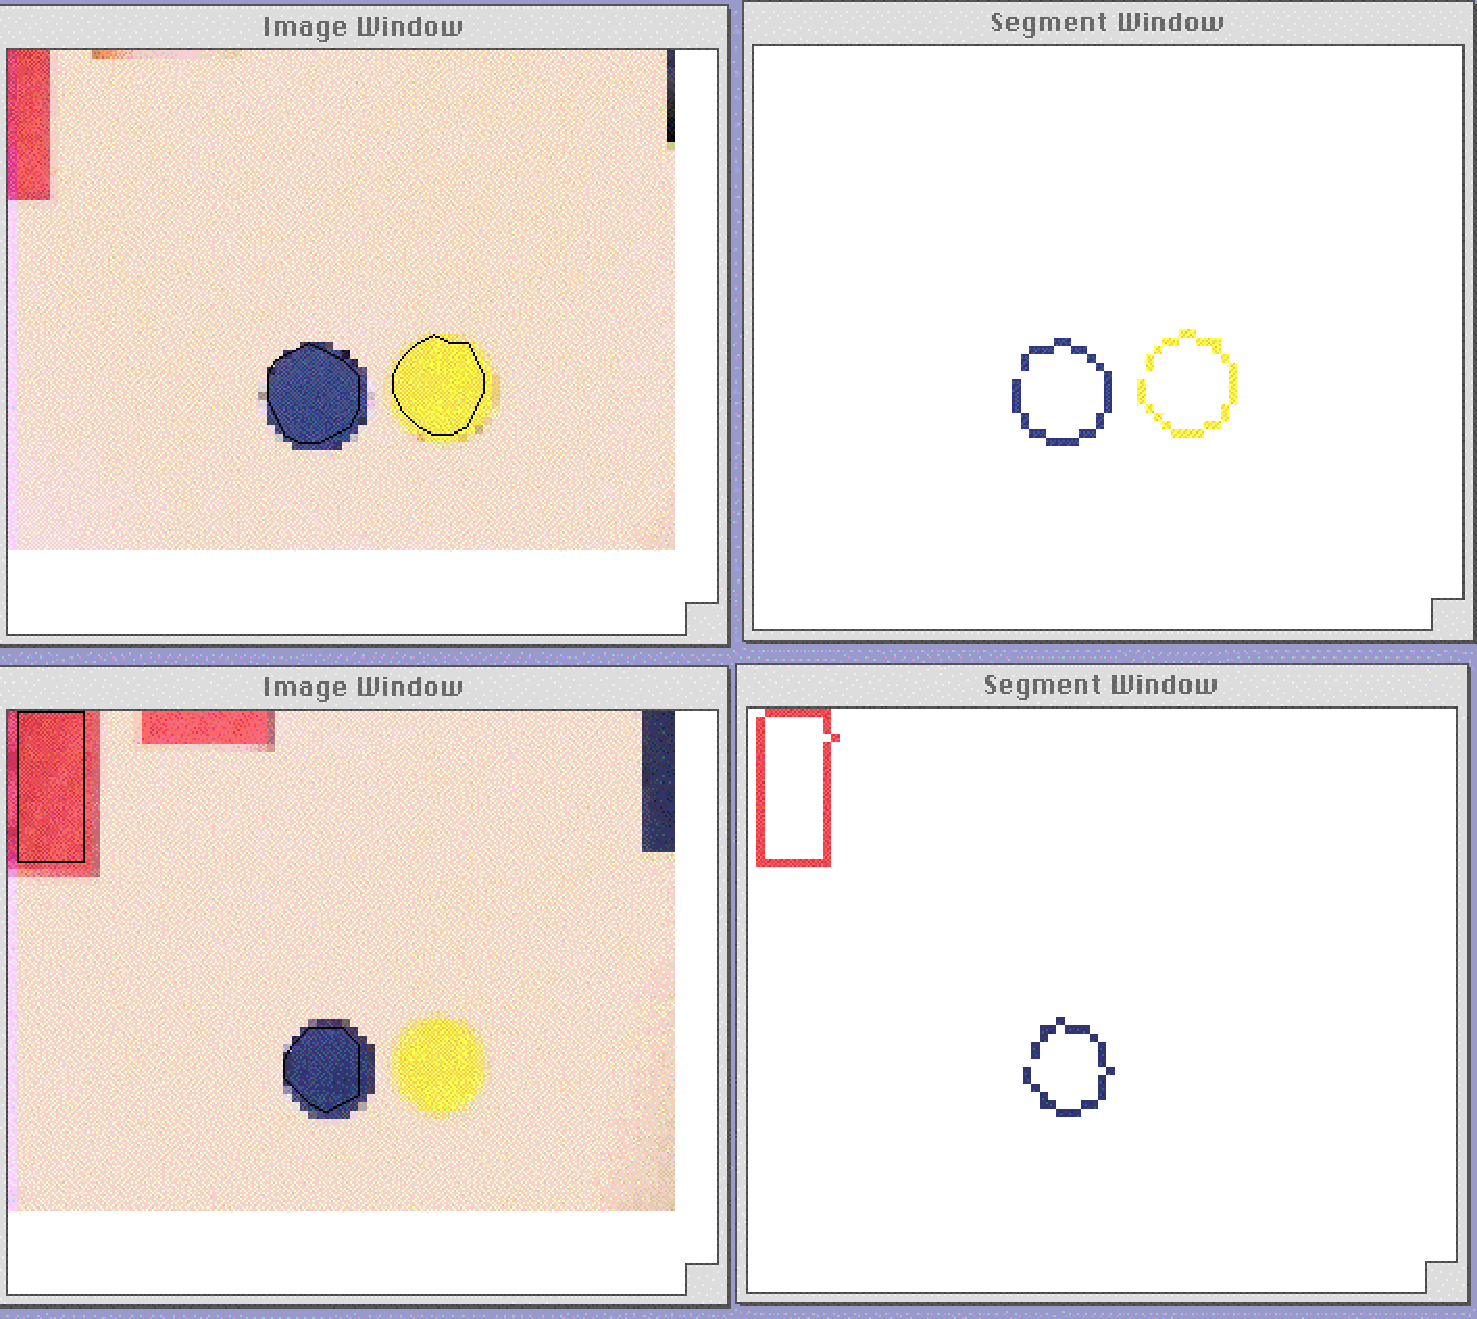
\includegraphics[width=.55\textwidth]{chap3/figs/diff-percept}}
\caption{ Top (left), image captured by the hearer. 
Bottom (left), image captured by the speaker. Because
both have a different view on the scene, the 
images diverge and consequently 
the segmentation (bottom and top right) diverges as well, in particular the yellow 
circle is not perceived by the speaker. In contrast the speaker perceives a rectangle
(bottom left corner) and has chosen this as the topic. The rectangle is not perceived by the 
hearer, so the game has no chance to be successful.}
\label{f:plate12}
\end{figure}

\subsection{The Sieve Architecture}

\is{sieve architecture}Segmentation exemplifies a dual kind of processing that 
we will encounter again and again as we focus on the 
different layers of the cognitive 
architecture (\figref{f:sieve}). 
Various possible solutions are generated, 
expanded and combined in parallel. The possible solutions enter
into competition until globally coherent
solutions emerge, which are ranked and handed to the 
next layer of processing. Often 
a solution does not emerge or multiple solutions are
equally valid in which case constraints from 
expectations or from the further processing of partial
solutions must flow down to influence `earlier' processing, 
which can be implemented as a `re-entry' of some solutions
back into the previous layer. For example, hearing a word may 
stimulate the expectation that a certain category is
relevant, which in turn may stimulate the computation
of certain features and influence how the image is 
segmented. A speaker may have to choose between alternative
segmentations and categorisations depending on whether 
the conceptualisation can be succinctly and accurately 
lexicalised and possible lexicalisations will only be 
acceptable when they can be integrated in a complete sentence. 
\begin{figure}[htbp]
  \centerline{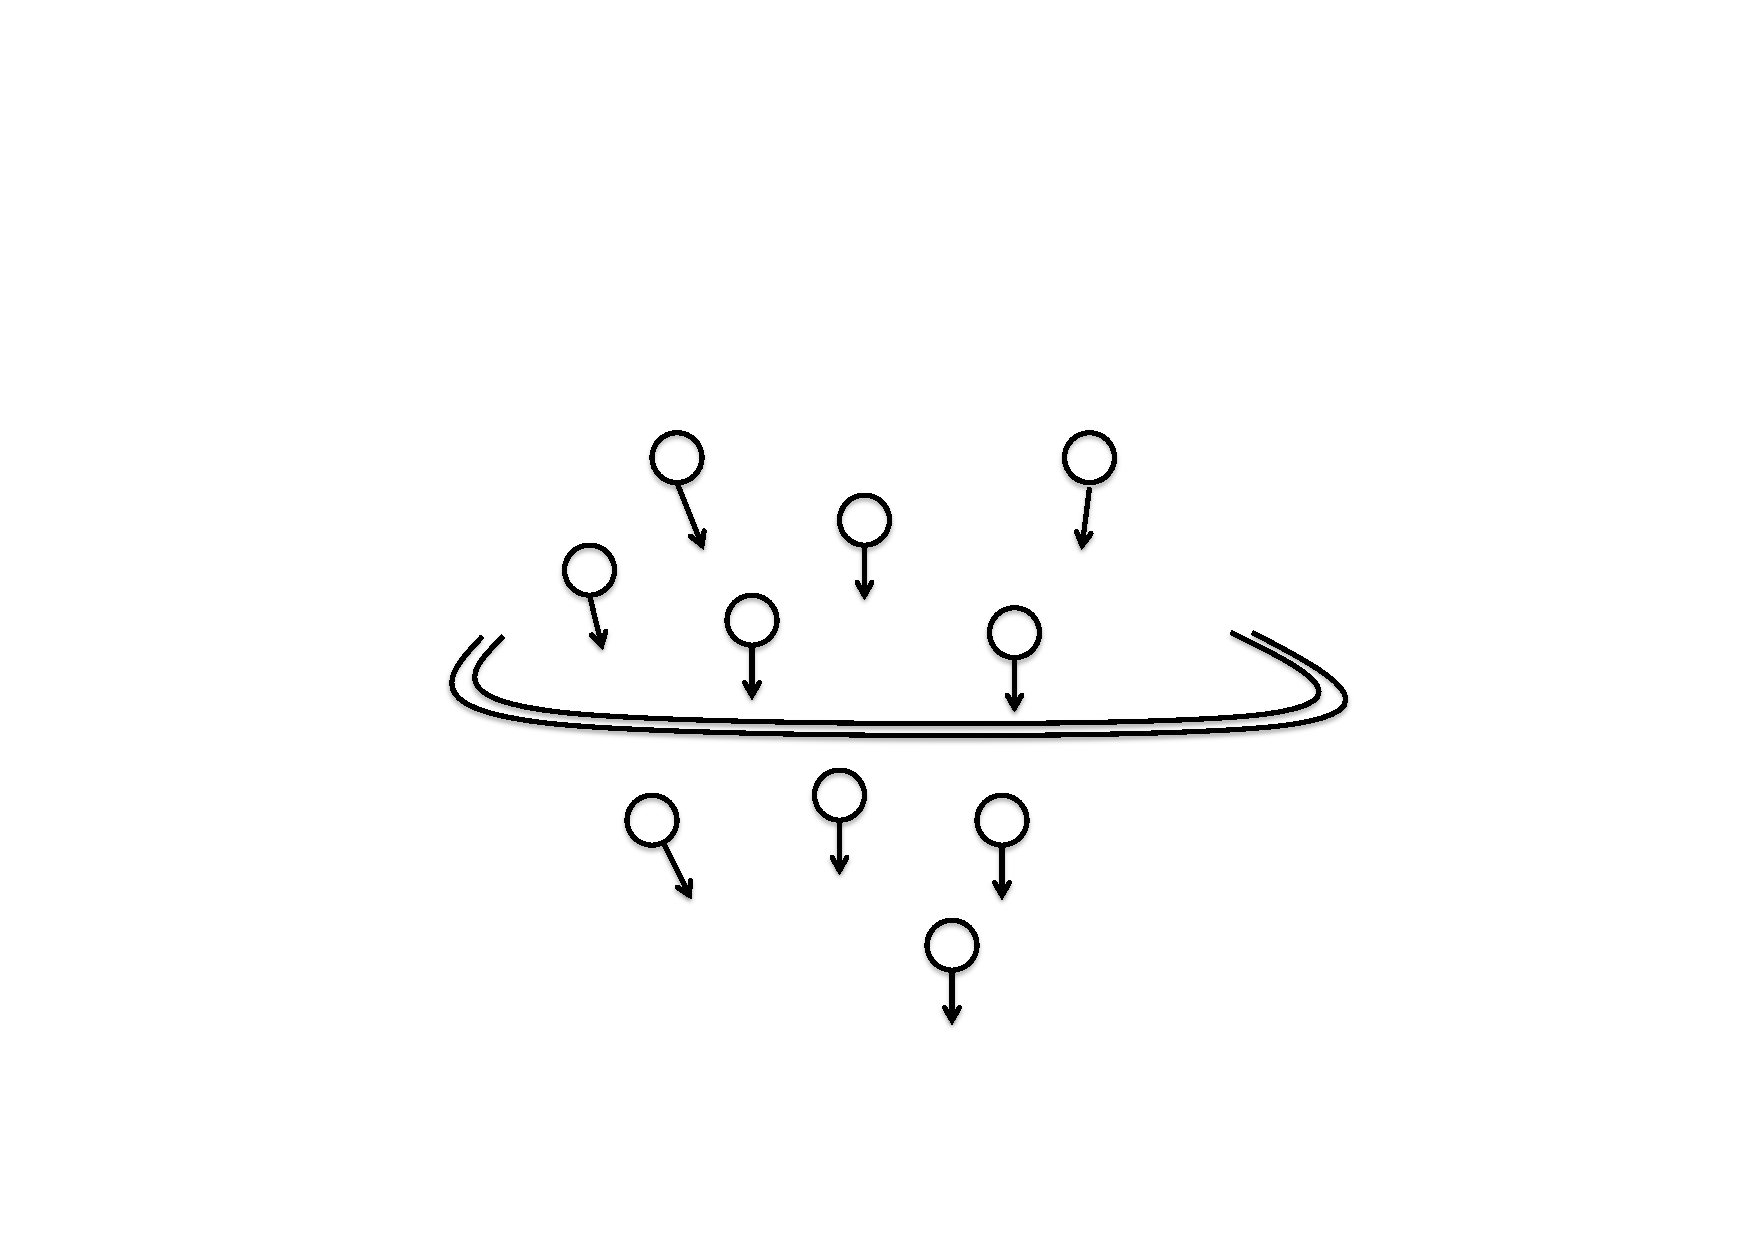
\includegraphics[width=.55\textwidth]{chap3/figs/sieve}}
\caption{\footnotesize The different layers of cognitive processing act 
like a sieve. Inputs flow into the layer, where they are processed
to generate hypotheses of which the best ones are transmitted
to the next layer. Every layer can operate in both directions, 
so that constraints can flow from top to bottom and from bottom
to top. \label{f:sieve}}
\end{figure}

The two way flow of constraints (from perception to 
high level cognitive processing and from high level 
cognitive processing to perception) suggests 
that the brain is best thought of as a massively parallel, 
densely connected processing system, in which multiple 
partial solution structures float up or down, gathering strength 
or weakening with new information entering the system. 
This contrasts with the view that 
information is processed in a serial step-by-step fashion
through tightly compartmentalised modules.\footnote{
See \cite{Fodor:1983} This book discusses a modular, sequential 
information processing architecture for cognition. A 
non-modular, parallel view 
is sketched in: \cite{Minsky:1985}. 
A more realistic neurophysiological model similar to the 
one underlying the `sieve architecture' we have used is
discussed by \cite{Edelman:1987}.} It is true
that we have the illusion that there 
is some {\it homunculus}, a little man, which sees a single coherent 
picture of reality and finds quickly the right way to 
verbalise or interpret this picture, but closer examination 
of the actual informational requirements of each subprocess
shows that this can never work. Constraints must flow in all 
directions, because the sensory data has not enough information to allow 
a unique segmentation, and categorisation and language is 
too full of ambiguities to allow a straightforward linear
interpretation. 

\section{Sensory Channels}

\is{sensory channels}Once segments have been found, further characteristics must
be extracted. The values of these various characteristics
will be communicated on sensory channels to later categorisation
processes. A characteristic property of a segment, such as 
average gray-scale, is still in the
analog continuous domain and should not be confused with
a category (like dark or light) which is in the
discrete symbolic domain. An open-ended set of possible sensory 
channels can be imagined, ranging from very general 
channels sensitive to often recurring properties relevant
in common tasks and thus shared by most people, to very 
specific channels which only experts in specific
domains possess. 

\subsection{Example channels}

The segment characteristics which will be 
used later in various experiments are defined below. 
Their values are all derived by straightforward computations from 
the raw image maps captured by the cameras. 
\begin{itemize} 
\item AREA: The surface area of a segment
is calculated by simply counting the number of pixels that are part 
of the segment. 
\item HPOS, VPOS: The x and y values of the 
central-position of a segment. The central position 
is calculated by taking the mid-point of the sides 
of the bounding box. 
\item HEIGHT: The height of the bounding box. 
\item WIDTH: The width of the bounding box. 
\item BB-AREA: The area of the bounding box,
calculated by multiplying height by width. 
\item GRAY: The average gray-scale value of the pixels
in a segment. 
\item R, G, B: The average R (redness), G
(greenness), and B (blueness) values in a
segment. To obtain more human-like colour channels, they are
transformed in terms of YB (yellow-blue), RG (red-green), 
BW (black-white), SAT (saturation) and BRIGHTNESS channels. 
\item EDGE-COUNT: The number of edges in
a segment, for example 3 in the case of 
a triangle. 
\item ANGLE-COUNT: The number of angles, determined on the 
basis of the junctions. 
\item RATIO: The ratio between the area of the segment 
and the area of its bounding box, which gives an idea how close 
a figure is to a rectangular shape. 
\end{itemize}

Each of these segment characteristics or combinations of
characteristics enables certain types of
categorisations. For example, the GRAY channel makes 
it possible to distinguish between 
light and dark, HEIGHT between short and tall, HPOS between 
left and right, VPOS between top and bottom, 
AREA between big and small, etc. In the next chapter, we will study 
how such categorisations may 
form on the basis of their respective channels. 

\subsection{Conceptual spaces}

\is{conceptual spaces}The sensory channels used in the experiments have
deliberately been kept to a minimum so that we can follow 
in detail the ontological and lexical dynamics, which is a 
non-trivial matter as I will demonstrate in chapters 6 and 7.
Obviously to get a richer lexicon, more channels need to be made 
available to the agents. These channels can often be 
grouped to form a `conceptual space'.\footnote{See \cite{Gardenfors:1999}
More cognitive oriented spaces, further removed 
from perception, are discussed in \cite{Fauconnier:1994}.} One of the 
best known examples is the colour space formed by the
yellow-blue, red-green, black-white, saturation, and brightness channels. 

Here are some other examples: 

1. A set of sensory channels that are sensitive 
to characteristics of moving segments can easily be 
imagined. They include the speed
of movement, the direction of movement (along the 
horizontal position (HPOS) and vertical position (VPOS) 
dimensions), or the change in area (getting bigger if the object 
approaches or smaller if it moves away). This is the foundation
for categories about spatial change: moving left versus moving right,
approaching versus retracting, speeding up versus slowing down.\footnote{Experiments
using segmentation based on movement
using the dedicated hardware shown in \ref{f:plate6} were carried out by Tony Belpaeme. 
More details can be found in: \cite{Belpaeme:1998} These channels have been used in
language experiments where the agents were 
perceiving and communicating about moving 
images: \cite{Steels:1998}  
The segmentation used in this book 
based on output from the Sony EVI-D31 camera was 
implemented by Danny Van Tieghem. Angus McIntyre integrated
the interfaces to this camera within the BABEL environment. 
}

2. Various spatial relations between segments can be computed: 
inclusion and overlap between segments, distance between 
midpoints, hierarchical structure, etc. 
This leads to another batch of categories which are
the basis for spatial distinctions like inside versus outside. 

3. More properties of the shape of segments can be computed.
I have already introdced the RATIO channel, which is the area of the 
segment divided by the area of the bounding box, giving an 
indication how rectangular a segment is. This can be generalised
by using an ellips around a shape so that we can calculate
convexity. We can then also calculate elongation (by calculating
the principal axes of the ellipse). 

It is not at all necessary that the channels operate 
on visual input, they can also use actuator sensors or internal states
like the level of the battery. It is moreover possible to 
consider channels for dynamic states, for 
example by transforming the sensor and actuator
data into state-space representations and 
analysing them in terms of attractors.\footnote{
Several examples of this type of approach are 
found in \cite{Port:1995}}

The ontological and lexical apparatus of the Talking Heads is 
generic with respect to the nature of the sensory channels
that are used, they could just as easily be about other sensory 
domains like sound, tactile sensation or internal states
of the robots.

\subsection{Perceptual Constancy}

\is{perceptual constancy}Real world sensory data is remarkably volatile due to the 
high variation and constant change of 
our physical environment, nevertheless human beings have 
the illusion of constancy. 
For example, the colour of an object is determined 
by the wavelength of the light reflected by its surface. 
For a long time, it 
was thought that colour was an intrinsic property of a 
surface, and that we therefore experience the colour of 
an object as constant, but psycho-experimental evidence has shown 
that this is not true. When we look at a surface in 
isolation which reflects light between 
430 and 470 nanometers, we experience 
the colour blue. As a result, one might assume
that blue can be equated
with the experience of light in this particular wavelength 
region. However, if the same surface is perceived
in a broader context and the light conditions 
are changed (so that objectively they now 
reflect light in a different spectral region), they still 
appear as blue! What should objectively 
appear green according to the measured wavelength 
values is still experienced
as blue. This explains why we see colours
as relatively constant even if the light conditions
are changing (for example from broad daylight to 
evening light) which is obviously extremely useful 
for dealing with rich environments. But it 
implies that colour is {\it not}
an intrinsic property that can be measured objectively 
with a light meter. It is actively mapped onto reality 
as a result of complex processing which takes the 
context into account.\footnote{
See the discussion about colour 
in: \cite{Varela:1991}}

The same sort of context-sensitivity\is{context-sensitivity} 
is important for the other sensory dimensions 
that the Talking Heads use, as well as for segmentation. An 
object will appear large or small depending on the 
other objects in the scene. It will appear light 
or dark depending on the average brightness. 
A scene may be segmented in one way or another 
depending on the objects it contains. 
Visual illusions arise when more than one context
is consistent with an image and interpretations sometimes
switch back and forth between different possibilities. 

\subsection{Transformations}

Cognitive agents can stabilise the sensory data to
achieve more perceptual constancy by transforming them so 
that the data become less context-sensitive. 
This implies that additional processing first recovers
more information about the context. 
One of the best known examples of this concerns
colour constancy. As mentioned earlier, wavelength 
reflection is strongly influenced by the background 
light in the environment. However, when the average surface 
reflectance is known, it is possible to transform 
the colour data to recover the colour that is 
experienced by humans as constant for a surface.\footnote{
See the discussion in: \cite{Zeki:1993}, particularly chapter 
23.}
 
\subsection{Scaling}

\is{scaling}The second way in which the erratic nature of 
real world signals can be diminished is by
scaling. Scaling means that 
the values actually recorded by sensors or
feature extractors are calibrated with respect 
to a frame of reference. 

A first frame of reference is based on
the absolute minima and maxima of the values 
on a sensory channel. This can be used to do 
{\it sensor-oriented scaling}. For example, 
the image map captured by the camera
contains 320 x 240 pixels, which means 
that the horizontal position (HPOS) has a value between
0 and 320 and the vertical position (VPOS) has a value 
between 0 and 240. Both values can be scaled to fall between 
0.0 and 1.0 so that they become uniform with respect to 
other sensory channels. Given a value $x$ and a 
$min$ and $max$ value, then the scaled value is 
$x' = {(x - min)}/{(max - min)}$. 
Thus the sensed value of HPOS=200 becomes
HPOS=0.62 after scaling . 

In the experiments discussed later, 
sensor-scaling is always performed so that all sensory data
is between 0.0 and 1.0, allowing values on different channels 
to be compared with 
each other. In addition, context-oriented scaling is performed.
{\it Context-oriented scaling} uses the minima and maxima of the 
values that effectively appear in the context.
For example, if the values for the HEIGHT of segments 
observed in the scene is between 500 and 700, 
then these can be the minimum and maximum of the 
HEIGHT scale, so that 500 maps onto 0.0 and 700 to 1.0. 
Context-oriented scaling acts like a lens
magnifying the perceived values so that distinctions
stand out more clearly. This scaling could 
be made more sophisticated by introducing an additional scaling factor so that 
differences are amplified but not necessarily blown up to their extremes. 

Context-oriented scaling has two advantages. The 
context is now strongly taken into
account, in a way similar to human perception: A segment
looks dark when surrounded by light segments but
light when surrounded by darker ones. The second advantage is 
that differences within the relevant subrange that 
actually occur in the scene are amplified, so that 
they stand out even if the range of possible values is
much wider. Often both relative (context-oriented) 
and absolute (sensor-oriented) scaling 
are pertinent. Thus `left' can be
the left-most of all the objects in the scene (context-oriented
scaling) or `left' in absolute terms (sensor-oriented scaling). 
Some channels, such as the colour channels, should never be scaled
for context, because the categorisation works best on the basis of 
the sensor-scaled values. 

Context-oriented scaling is not necessarily based on the 
frame of reference imposed by the image map which is 
recorded by perceiving the scene from the viewpoint of 
the camera. Many contexts and hence other frames of reference
are possible and are exploited in natural language 
conversations. Often a particular context is communicated through 
language. Scaling is then performed within the
frame of reference suggested by that context, 
for example, if I will tell someone "the chair is to
your left", whereas it may perhaps be to the right of the
hearer from my point of view. 

A final form of scaling uses the typical values of the object being 
perceived. I will call this {\it object-oriented scaling}. 
For example, a small elephant is always
very large next to a large mouse. We clearly
have expectations about the typical size of an elephant at
a certain distance and use it to scale
perceptual data prior to size 
categorisation. Context-oriented and object-oriented scaling
are examples how constraints must flow 
from non-visual cognitive processes to visual processing. 
These non-modular interactions are a strong
indication that cognitive subsystems must be highly 
interconnected. 

\subsection{Saliency}

\is{saliency}The perceptual layer generates in parallel a wealth of 
sensory characteristics about each of the segments in 
an image and their relationships. But not all sensory 
characteristics are equally distinctive. For example, two 
segments in a scene may have almost the same area but 
one might be very thin and thus tall, and the other very wide
and thus short. In our own human perception, those channels
that reflect significant differences stand out and are preferred
in referring to an object. Therefore, it is unlikely that area would be 
used in \figref{rect1b} to distinguish object 1 from 
the others. 
\begin{figure}[htbp]
  \centerline{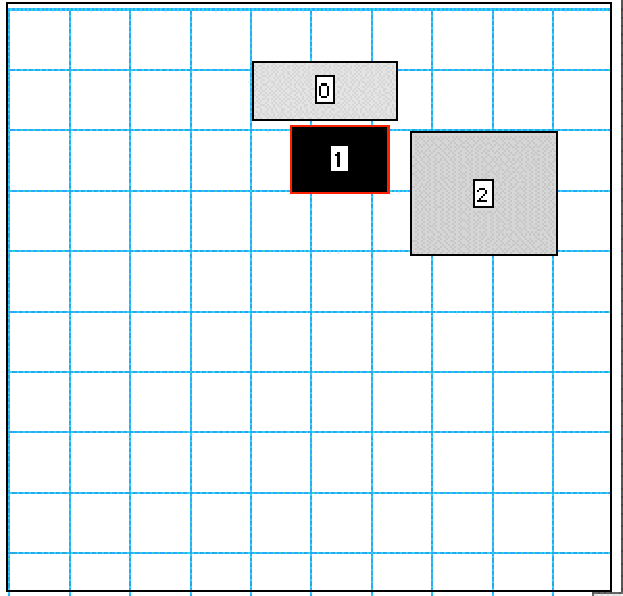
\includegraphics[width=.45\textwidth]{chap3/figs/recscene}}
\caption{\footnotesize \label{rect1b} A scene with three objects. The
sensory values on the grayscale channel are the most salient 
and will therefore be chosen preferentially for categorisation
and verbalisation.}
\end{figure}

The saliency of a channel 
is the smallest distance (after sensor-scaling) between the perceived
values of the topic and one of the corresponding perceived values of the 
other segments in the context. 
Thus the different perceived values (after sensor-scaling)
for the segments in \figref{rect1b} are shown in 
\tabref{tab:rect1b}. The last line shows the saliency, assuming that 
the topic is segment 1.  Clearly the GRAY-channel is the most salient
one in this case, followed by the WIDTH-channel. Other 
sensory channels such as HPOS, VPOS or HEIGHT (which have almost the same 
values for object 0 and 1) are not salient at all. 

\begin{table}
\begin{center}
\begin{tabular}{  l   l   l   l   l   l   l  } \midrule
{\it obj} & HPOS & VPOS & HEIGHT & WIDTH & GRAY & AREA \\ \midrule
0 & 0.66 & 0.95 & 0.01 & 0.71 & 0.19 & 0.27\\ \midrule
1 & 0.69 & 0.83 & 0.07 & 0.33 & 0.97 & 0.21\\ \midrule
2 & 0.99 & 0.87 & 0.54 & 0.72 & 0.22 & 0.57\\ \midrule
sal & 0.03 & 0.05 & 0.07 & 0.39 & 0.75 & 0.06 \\ \midrule
\end{tabular}
\caption{Perceived values for each segment in \figref{rect1b}.
\label{tab:rect1b}}
\end{center}
\end{table}

Determining saliency has to be done before context scaling, because
context-scaling stretches the values to their extremes and so 
saliency information is lost. 
\tabref{tab:rect1b-area} below shows for the scene shown in
\figref{rect1b} the AREA channel with its
raw data, the value after 
sensor-scaling (with minimum 1,000 and maximum 
10,000), and the value after context-scaling. 
\begin{table}
\begin{center}
\begin{tabular}{  l   c   c   c  } \midrule
{\it Object} & {\it Raw data} & {\it Sensor-scaled} &  {\it Context-scaled} \\ \midrule
0 & 24530 & 0.27 & 0.18 \\ \midrule
1 & 18924 & 0.21 & 0.0\\ \midrule
2 & 50960 & 0.57 & 1.00 \\ \midrule
\end{tabular}
\caption{Data for the area channel for the scene in \figref{rect1b}.
\label{tab:rect1b-area}}
\end{center}
\end{table}
\begin{figure}
\begin{center}
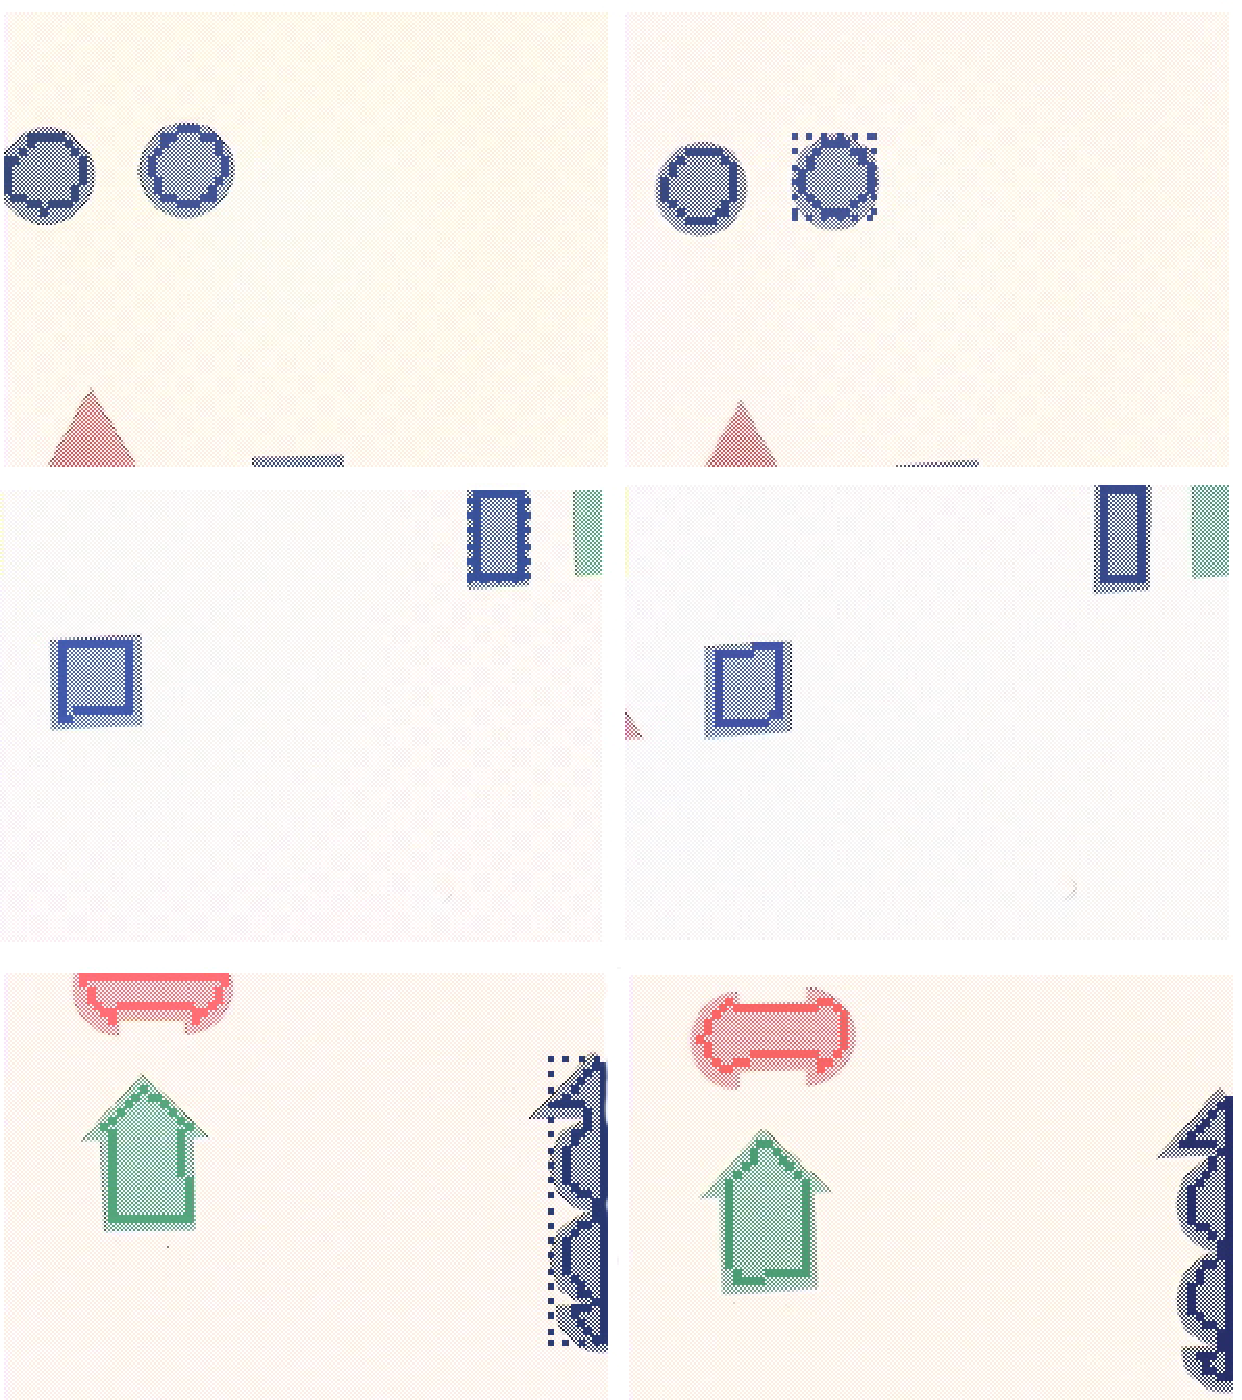
\includegraphics[width=0.8\columnwidth]{chap7/figs/plate-10}
\end{center}
\caption{Three examples of segmented images. The 
topic is indicated by a dashed bounding box in the 
image of the speaker. Segments which are too small 
are ignored. The topics have all been conceptualised
as being `to the right' and so the same word 
"gofubo" has been used to refer to them. }
\label{f:plate-10}
\end{figure}

Another example based on the segmented image is shown in Figure 
\ref{f:plate-10} (top images). Two circular segments
have been identified, the others are ignored because they are 
too small. The different sensory values (after sensor-scaling)
for the segments in the speaker's image are shown in \tabref{tab:t-plate10}. 

\begin{table}
\begin{center}
\begin{tabular}{  l   l   l   c  } \midrule
{\it channel}& {\it obj-0} & {\it obj-1} & {\it saliency}\\ \midrule
HPOS & 0.27 & 0.16 & 0.11\\ \midrule
VPOS & 0.20 & 0.20 & 0.0\\ \midrule
HEIGHT & 0.15 & 0.15 & 0.0\\ \midrule
WIDTH & 0.10 & 0.11 & 0.01\\ \midrule
AREA & 0.10 & 0.10 & 0.0\\ \midrule
R & 0.23 & 0.25 & 0.02\\ \midrule
G & 0.32 & 0.34 & 0.02\\ \midrule
B & 0.63 & 0.65 & 0.02\\ \midrule
\end{tabular}
\caption{Perceived values for each segment in \figref{f:plate-10}
\label{tab:t-plate10}}
\end{center}
\end{table}

The table shows clearly that HPOS is the most salient channel. 
The horizontal position also strikes us immediately 
as being the most salient when looking at plate [game2]. 
For many of the other channels, the differences are
almost insignificant. The use of saliency facilitates 
enormously communication and the acquisition of new categories. 
The case shown in plate 10 (top images) is an excellent opportunity 
for the agents to learn about left versus right. If more 
channels are salient, it is no longer so easy for the 
hearer to guess what meaning might have been used by the 
speaker and so incoherence would slip into the group's lexical
system. 

\begin{figure}[htbp]
  \centerline{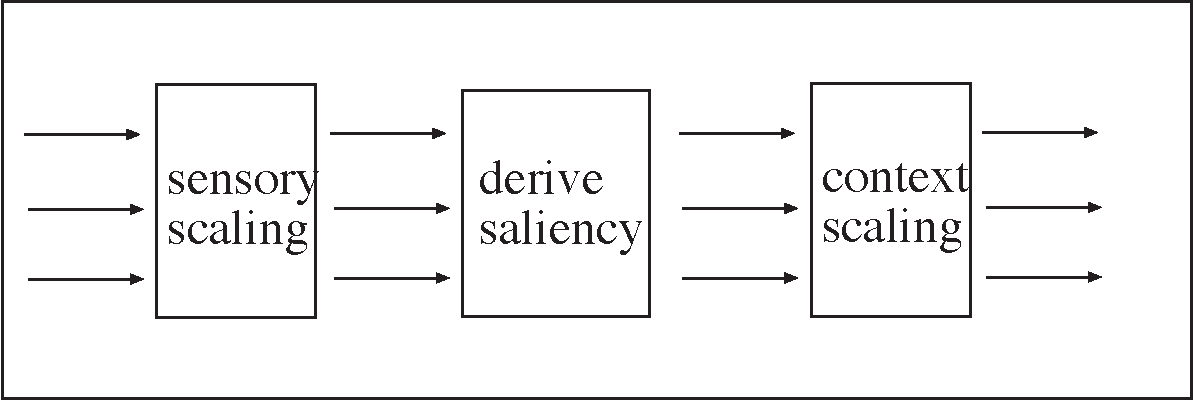
\includegraphics[width=.65\textwidth]{chap3/figs/scaling}}
\caption{\label{scaling} Processing converts data on 
a sensory channel into more usable data for later categorisation processes.}
\end{figure}

The various steps that the agents go through
in preparing data on sensory channels are summarised in \figref{scaling}.
It is presented here as flowing in one direction, but in fact 
constraints coming from higher level cognitive processing may 
influence these steps. For example, if we say "the largest square 
left of the triangle", we expect the hearer to scale the squares
with respect to all the objects left of the triangle, not with 
respect to all the objects in the scene. The backward flow of 
constraints will be studied after I have covered the different 
layers separately. 

\section{Methodology}

I hope the reader now has a much better idea of the enormous challenge
that the Talking Heads face when trying to play a language 
game about a real world scene, particularly
because they try to develop a lexicon and ontology 
as well. The images contain a multitude of ways 
to make distinctions and they differ slightly for both agents. 
It is enough fo a cloud to pass by causing the light conditions
to change slightly, and different values are immediately seen 
on the colour channels possibly leading to different segmentations.
So how can the agents ever get a repertoire of abstract categories and 
associated words when the real world shows such a perplexing 
variation? Very different scenes (for example the ones contained
in plate 10) can intuitively be distinguished with the same 
categories (namely [LEFT] versus [RIGHT]). But how can such 
inductive leaps be made? Scaling and sensor transformation 
introduce some perceptual constancy, and saliency helps to 
restrict the attention to those
channels that are potentially effective in communication, but there 
is clearly an enormous gap between sensory data and language. 

In this book, I will 
not only report on the outcome of an experiment and 
what we learned about the nature of cognitive architectures, but 
I will also try
to illustrate how we tackle such tremendously complicated problems. 
I will take a moment to explain this methodology because it runs like 
a red thread through the remaining chapters of this book and 
differs from the way other subdisciplines of cognitive science 
go about their investigations. 

\subsection{Putting up scaffolds}

\is{scaffolds}The standard means of attacking a difficult problem is to 
break it up in subproblems. In this case, the most obvious
subdivision is along the different sides
of the semiotic square I introduced in the 
previous chapter (\figref{square}). This 
leads to three natural subproblems: perception, conceptualisation, 
and verbalisation. When breaking up a problem, we can initially assume that the 
other subproblems will be solved somehow and that they give perfect
output to the others
or provide the right feedback. We can then try to invent a mechanism that
can do the job for the subtask we are investigating in these ideal circumstances, 
and test its strength and limitations. This is like putting up
scaffolds to see whether partial solutions work, before putting 
it all together. 
\begin{figure}[htbp]
  \centerline{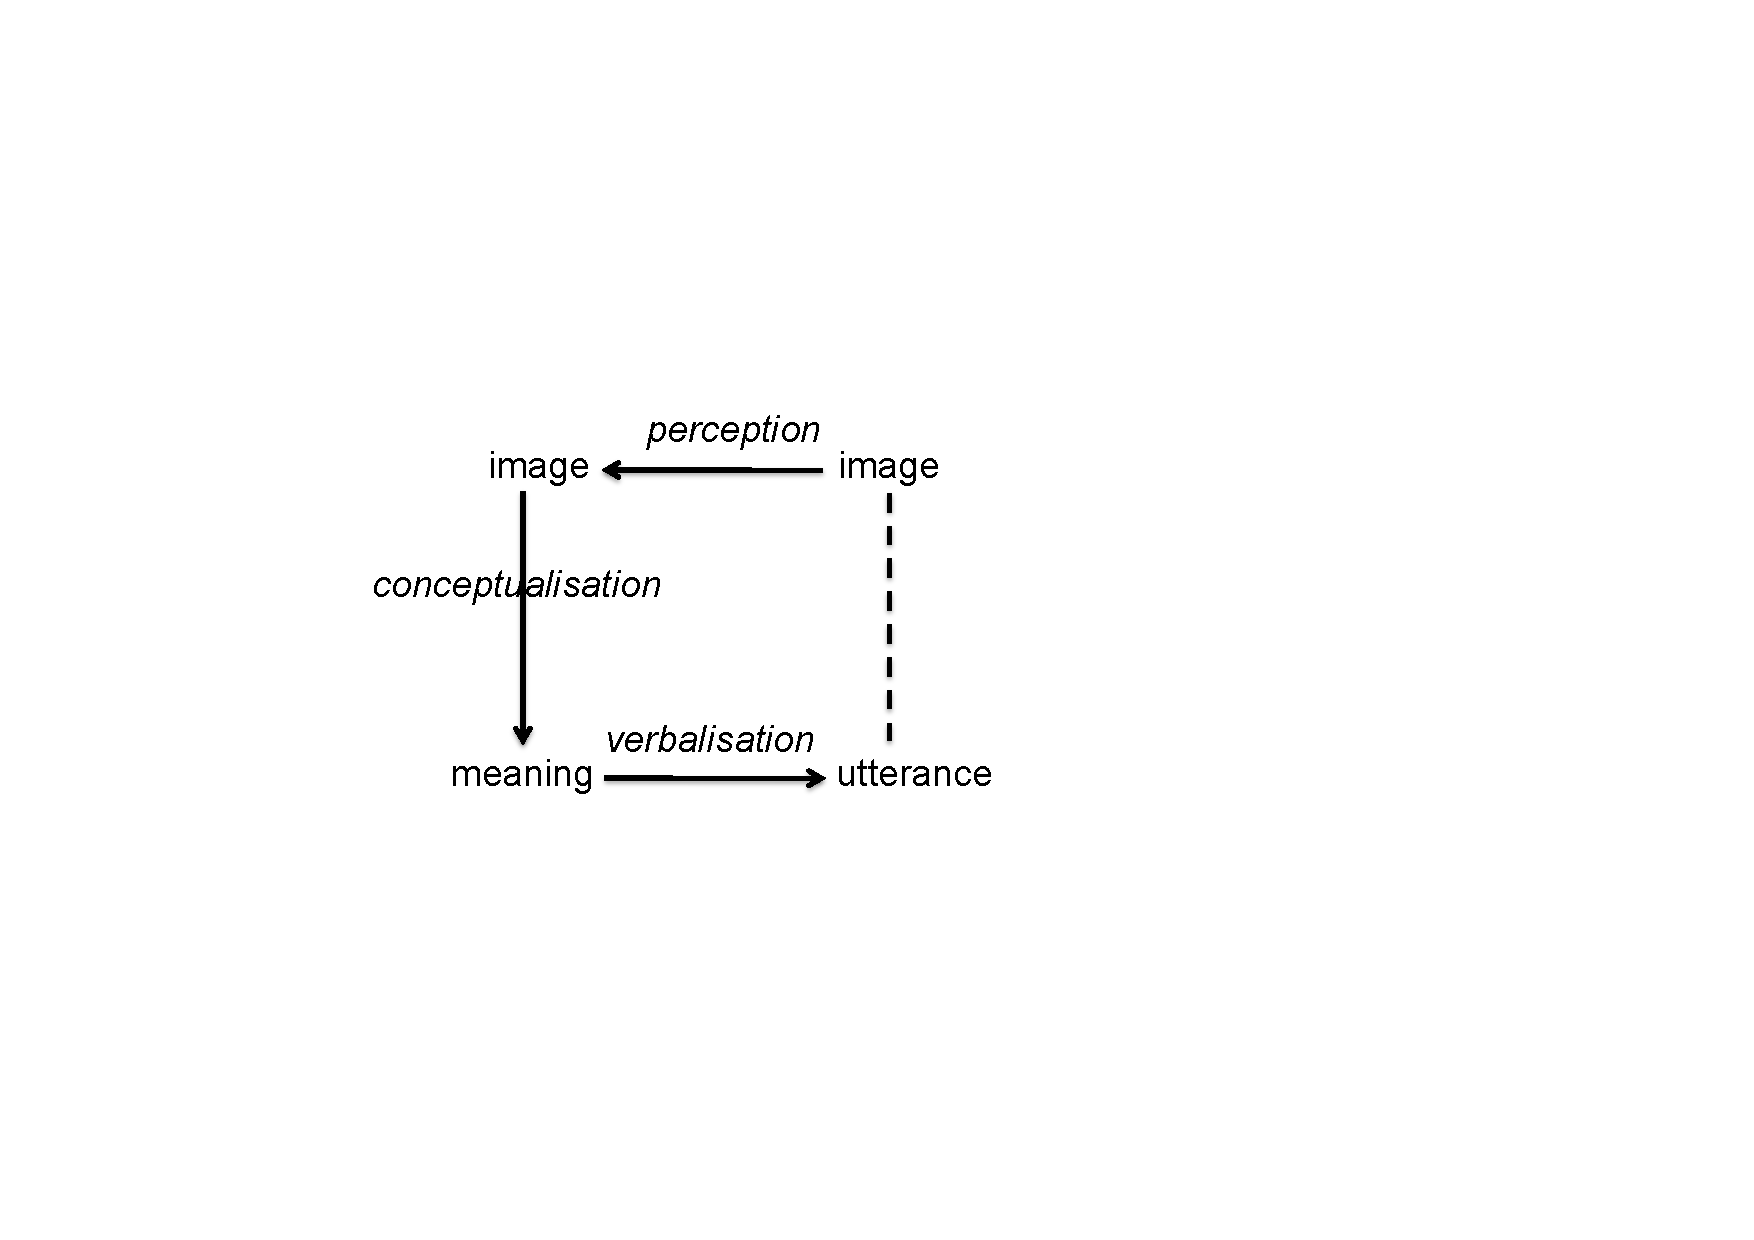
\includegraphics[width=.50\textwidth]{chap3/figs/square}}
\caption{\label{square} The general problem of 
production is broken up into three subproblems: perception, 
conceptualisation and verbalisation.}
\end{figure}

I will extensively make use of this methodology. 
This chapter has focused on perception, the next chapter focuses
exclusively on
conceptualisation, assuming that there is good segmentation and a 
decent set of sensory channels. Chapter 5 turns to the 
problem of lexicalisation, assuming that 
the agents have a shared repertoire of meanings and agree on 
what meaning to use in a particular game. Chapter 6 then puts the solutions 
for conceptualisation and lexicalisation together by coupling their
inputs and outputs and establishing the appropriate feedback connections. 
Chapter 7 then couples this system to the perceptual processes discussed
in this chapter, so that we get back to our 
original goal: understand how perceptually grounded language communication 
is possible. 

The methodology of breaking a problem into its subproblems goes quite 
a distance, but is not without danger. The processes relating
perception to language cannot be modular for reasons already mentioned. 
Each layer receives inputs which are not completely reliable and 
generates a set of possible suggestions rather than a single
`correct' solution. Constraints have to flow
from top to bottom because there is simply not enough reliable 
information to solve the problem with a straightforward sequential 
decision process. In addition, every layer is constantly adapting 
itself to the surrounding information context. New categories 
may develop, new words need to be learned, new sensory 
channels may even emerge. So, constructing a global system is going 
to be more than simply putting together its parts. There are complex
behaviors that will only become visible when the appropriate non-modular
couplings are put in place, and this is notoriously difficult to 
do and study. 

\subsection{Idealisation and realism}

To make this problem more manageable I will 
adopt a second complementary method, widely used in
engineering. We can keep the various
aspects of the global process intact, but simplify the challenge. 
We start with extremely idealised operational circumstances
and then gradually add more and more realism, until the system is 
ready to face the real world. At every step we first establish
whether the mechanisms still work, which means in the guessing
game that communicative success moves up. If this does not happen, 
we must investigate what needs to be added or changed and perhaps
reduce the complexity again to find a new bottom ground. 
If a language system does get established, we can examine 
the limits of the process before increasing the challenge once more.
During the original research, 
we extensively used this stepwise approach, often `sliding down the 
mountain' when too much complexity was introduced too quickly so 
that we were forced to take a few steps back and tackler simpler 
challenges until we got our feet on the ground again. 

We can simplify or scale down in four dimensions. 
The first dimension is that of the agents. I 
will often start by investigating a group of only two agents, then scale up
to larger and larger groups, 
and then tackle the problem of an open-ended population in which 
new members enter and others leave. Each of these steps 
introduces additional difficulties. For example, when there are
only two agents, the risk of synonyms forming is low - as we 
will see later - because the agents only interact with each 
other and so they can rapidly see whether the other one has
a word for the same meaning. But when the population is scaled up 
it is highly likely that different subgroups invent 
different words or develop new meanings.
These variations take time to propagate until
the group settles into a coherent state. 
When there is an open-ended set of agents, the new agents
in the population must acquire a language which already 
exists, which implies that we must have demonstrated that language 
acquisition goes sufficiently fast to explain cultural 
transmission. When agents leave the community, they take some
of the knowledge of the language conventions, and so we have 
to show that the whole community might destabilise. 

Second there is the dimension of the real world and how it relates 
to perception and action.  For this book, I will in any
case only use worlds restricted to 
coloured shapes on a two-dimensional surface, thus drastically reducing
the perceptual challenges, and constrain the perceptual 
task still further by supplying the agents only with a 
limited set of sensory channels. We also performed
initially many simulations with artificial worlds (to
be explained shortly) where we could carefully control various 
parameters, such as the number of objects in a scene, their
complexity, or their variation. 

But restricting the environment 
is not enough. Other aspects of perception
can seriously disrupt language communication 
in a variety of ways and each of them can be neutralised. 
We have already seen that 
in normal circumstances, the agents 
do not share the same image of reality, which introduces 
a whole array of problems. They might consequently
segment the scene differently, the pointing might not be accurate enough
(even if they both were referring to the same object), 
the segments might have very different sensory characteristics 
(as already discussed for plate 12). We have
reduced these sources of difficulty by initially using 
only one camera, then scaling up to two cameras
in the same room, and only then scaling up to many different cameras
located all over the world. Increasing or decreasing the importance 
of saliency also helps. When only the most salient sensory 
channel is used, agents have a higher chance to guess the 
right meaning (at least if their perception converges reasonably 
well), and so they can better guess the meaning of an unknown
word or go less astray with words for which they have already
a shared meaning. So by varying the saliency, we can control the 
degree of semantic ambiguity in the agents' communications. 
Divergent perception and confusing regularities in the
environment are sources of 
polysemy in language, which the agents need to 
dampen if they want their communications to be efficient and
reliable. 

Another real world aspect that we can make more or less
complex is related to the movements of the head and the pointing. 
A hearer must be able to look in the same direction as the 
speaker, so that there is a minimum shared context. The 
hearer must be able to point to the topic guessed, 
so that the speaker can see whether the communication 
succeeded. If it did not, the speaker must be able to point 
to the topic. These physical interactions are well within
the state of the art in robotics, and there exist even 
various learning systems capable of bootstrapping this capacity
from scratch.\footnote{
This is the problem of hand-eye coordination performed
in living systems by the vestibulo-oculomotor systems. 
See: \cite{Anastacio:1989}.}

But these processes will never be completely 
reliable either. So we can increase or decrease the challenge
to the agents by making the non-verbal communication and 
coordination more or less challenging. In the experiments 
reported in this book, speaker and hearer can communicate to each 
other the direction in which they 
are looking.\footnote{
This real world interaction has been developed 
by Frederic Kaplan \cite{Kaplan:1999}.}
Because they still see a 
different image due to their physical position, the 
interaction is still partly unreliable but it is sufficiently stable 
to enable the agents to bootstrap a shared communication
system, which then in turn can help to establish 
physical coordination. 

Third, there is the cognitive apparatus of the agents
implicated in language. Here we can start with a simple 
associative memory for the lexicon 
that can only handle single words
associated with single meanings, and then scale up to 
conjunctions of meanings covered by single or
multiple words, and then still further to open-ended
complex meanings and syntax. 
Each step requires additional machinery in the agents, 
which will automatically lead to more complex linguistic
forms, but it is our experience that there is great value in
trying to understand the basic process of word 
meaning acquisition before attempting to install more 
cognitive complexity in the agents' architecture. Even for the
acquisition and propagation of single word utterances there are 
still many open-ended problems. 

A final dimension concerns the transmission and 
perception of the utterance. Here again we can scale
up or down the challenge to the agents, from full-blown 
unconstrained speech in noisy environments down to perfect direct
transmission of the language form by the 
speaker and perfect recognition by the hearer. 
Complexity along this dimension has been reduced to 
the minimum in the Talking Heads experiment. Agents 
transmit utterances directly although a speech sound
is generated so that human listeners can hear which
utterance is produced as part of a game. 

\section{The GEOM world}

\is{GEOM world}One way to perform controlled experiments 
quickly and on a large scale, consists of artificially 
generating the perceptual input to the agents. 
This has the additional advantage that we can 
simplify the situations the agents have to work in
(for example have fewer types of shapes) 
and let them start initially with a shared perception. A 
simulation world that we have used extensively 
for many simulations reported later 
is the GEOM world. 

The GEOM world generates geometric shapes similar 
to the physical figures we paste on the white board. 
Possible geometric shapes are circles, triangles, 
squares, rectangles, etc. 
We can control the complexity
of the scenes that are generated  through a few parameters, for example the 
number of minimum or maximum figures, or the possible 
repertoire of shapes. We 
ignore colour and use only different grayscale 
values. To construct a scene the computer simulation 
program chooses first a random number of 
figures. Then for each figure, a shape is 
chosen, and random values for the main 
characteristics (position, height, width, grayscale)
are set. 
\begin{figure}[htbp]
  \centerline{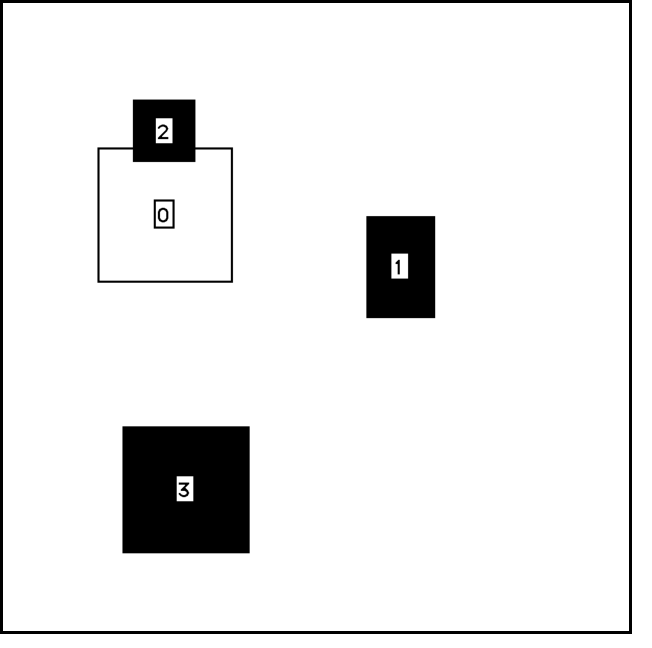
\includegraphics[width=.45\textwidth]{chap3/figs/scene9}}
\caption{\footnotesize \label{geom3} An example of the 
computer-generated scenes from the GEOM world.
Each shape is labeled for further reference.}
\end{figure}

An example of a computer-generated 
scene containing only rectangles is shown in 
\figref{geom3} (another one 
was shown earlier in \figref{rect1b}).
Given such a scene, each agent calculates
the bounding box and the segment-characteristics
for every computer-generated figure.
For the scene in \figref{geom}, which contains three
squares and a rectangle, the values of the channels
are summarised in \tabref{tab:t-geom}. 
\begin{table}
\begin{center}
\begin{tabular}{  l   l   l   l   l   l   l   l  } \midrule
 & {\it HPOS} & {\it VPOS} & {\it HEIGHT} & {\it WIDTH} & {\it GRAY} & {\it RATIO}  & {\it AREA} \\ \midrule
0 & 116 & 166 & 293 & 293 & 0.777 & 1.0 & 85849 \\ \midrule
1 & 692 & 317 & 148 & 224 & 0.449 & 1.0 & 33152 \\ \midrule
2 & 192 & 64 & 137 & 137 & 0.408 & 1.0 & 18769 \\ \midrule
3 & 167 & 770 & 277 & 277 & 0.201 & 1.0 & 76729 \\ \midrule
\end{tabular}
\end{center}
\caption{\label{tab:t-geom} Sensory data for the scene shown in \figref{geom3}.}
\end{table}

After sensory-scaling we get \tabref{tab:t-geomscaled}. 
\begin{table}
\begin{center}
\begin{tabular}{  l   l   l   l   l   l   l   l  } \midrule
& {\it HPOS} & {\it VPOS} & {\it HEIGHT} & {\it WIDTH} & {\it GRAY} & {\it RATIO}  & {\it AREA} \\ \midrule
0 & 0.09 & 0.13 &  0.64 &  0.64 &  0.78 &  1.0 & 0.95 \\ \midrule
1 & 0.55 & 0.25 & 0.16 & 0.41 & 0.45 & 1.0 & 0.37 \\ \midrule
2 & 0.15 & 0.05 & 0.12 & 0.12 & 0.41 & 1.0 & 0.21 \\ \midrule
3 & 0.13 & 0.62 & 0.59 & 0.59 & 0.20 & 1.0 & 0.85 \\ \midrule
\end{tabular}
\end{center}
\caption{\label{tab:t-geomscaled} Sensory data after scaling for the scene shown in \figref{geom3}.}
\end{table}

The output of the simulation is exactly the same as the one from real vision 
so that we can easily switch between simulation 
and physical experimentation. 

\subsection{Simulation versus experimentation}

Working with simulations has obvious advantages for 
speeding up development and systematic testing, 
but it does not replace experimentation with 
physical robots. It is true that 
building an experimental apparatus such as we built
for the Talking Heads experiment is a very 
non-trivial engineering project, particularly because 
of the teleporting infrastructure that enables the agents 
to travel to multiple sites and thus 
experience different physical environments or the same 
environment from different points of view. 
One might therefore wonder why we have persisted
to go to such great length in constructing
a real-world physical infrastructure. Why are
experiments with robotic agents necessary or 
desirable? Is it not enough to conduct simulation
experiments given that they can be done so much 
more easily? 

Computer simulations calculate the consequences of a
theoretical model. For example, we can implement Newton's
model of the solar system and simulate the movements
of the planets around the sun by calculating for 
small time steps the position of each planet and hence
the trajectories they follow. All the aspects of 
a calculation are under the scientist's control and it 
is therefore possible to use this method to examine whether a theory can 
be operationalised, whether it is coherent, and whether 
it is complete, i.e. whether it covers all 
aspects of the phenomena one tries to understand. 
Simulations can be inspected, re-executed
or reprogrammed by anyone who cares to challenge them and
other researchers can try to achieve the
same performance with alternative approaches, so that 
different theories can be compared in an objective way. 

Computer simulations can be set up for any theory which 
is formalisable, and hence for theories of cognition
and language as well. We need to implement the cognitive architecture
of the agent and then examine what happens when the agent
engages in interactions, i.e. when data is supplied from 
real or simulated scenes. Computer simulations of cognitive mechanisms
provide proof that they can be instantiated
on physical systems, even though it may still be
a mystery how the brain, 
itself a physical system, implements similar mechanisms. 
Computational simulation is of course 
not restricted to the theories I put forward in 
this book. Any theory claiming
to explain the origins of language and meaning 
should be testable by computer simulation, so that 
it is clear what form the architecture takes and whether
it does the job. All this is a big step compared to 
the early days of cognitive modelling when one was
supposed to believe on faith whether a certain cognitive
architecture could be instantiated by a physical 
system and whether it was indeed able to exhibit the functionality 
that was ascribed to it. 

But computer simulations have two major shortcomings, 
which makes them only one of the tools in the toolkit 
of the cognitive scientist. First of all, computer simulations by
themselves do not empirically validate a theory. When 
a computer screen shows pictures of planets moving around 
the sun, there is nothing that says that this is also 
the way the planets move. To validate the theory, large amounts of
data need to be collected of
the natural phenomena, and the simulation 
results have to be compared with the real world data to determine a sufficient
fit. In this book, we are primarily concerned with 
formulating new plausible models for cognition and particularly
for the origins of cognition, not yet with their
empirical validation; this exciting work is left for the future. 

However, there is a second shortcoming. Cognitive systems
must deal with the real physical world in its infinite variety 
and complexity. If we perform only computer simulations, 
we not only model the cognitive mechanisms of the 
agents but also the environments which they are 
confronted with. We validate the model only with 
respect to stylised worlds. Of course we can make
such worlds much more sophisticated, but 
there is never a guarantee that they are going to be
representative of the real worlds that
embodied cognitive agents have to deal with. 
The more realistic computer simulations 
become, that is the more aspects of reality they reliably 
take into account, the more the simulation starts to approach 
reality and the more a simulation may tell us whether
the proposed mechanisms live up to realistic circumstances.
But there will always be a huge difference between 
computer-simulated worlds and real worlds, as any
roboticist knows all too well. 
And this is why we need to do experiments
with physical robots and real-world environments. 

Of course, it is useful and efficient to 
conduct simulations as part of the discovery process 
but true validation of a cognitive architecture 
can only come when 
the system is confronted with a real physical environment. 
It forces us to attack the final known or hidden 
assumptions in the theory's operational validation. It
forces us to address the issue of sensing, using
real world physical sensors. Therefore, an experiment 
like the Talking Heads experiment has
a much greater force in 
convincing the sceptic. It is like testing the design 
for an airplane by building and flying one, as opposed
to demonstrating the idea only in simulation. 

\section{Conclusions}

This chapter focused on the perceptual layer which 
is responsible for interfacing the external physical 
world with the internal world of the agents. The 
interface is based on sensors to transduce external states
into internal states and actuators to transduce internal states into
external states. Four sorts of operations take place 
on raw sensory data making them more amenable to 
categorisation, conceptualisation and consequently 
language communication: Features in the 
form of micro-structures are extracted, the image is 
segmented in coherent units using region growing or 
countour finding, segment characteristics such as 
average colour or size are derived, and characteristics 
are transformed or scaled to bring out salient 
features and aid to achieve categorial constancy. 

The Talking Heads use 
standard techniques from computer vision research. Research
in this field is indeed so advanced that a large number 
of algorithms for segmenting images and extracting information about
image segments could be taken "off the shelf" and re-programmed to get 
a vision system that is adequate for the task setting 
of the Talking Heads experiment. This will, of course, no 
longer be the case if the environment is made more challenging
and more open to novel situations. Very quickly we would 
then reach the limits of what can currently be done using
standard techniques. Nevertheless for our purpose of 
exploring language and meaning, the Talking Heads 
vision system gives 
a sufficiently rich and reliable segmentation and 
characterisation of the scene so that an investigation
of how real world scenes might be conceptualised and 
verbalised, has become possible. 

%\documentclass{../_combined/fcg-book}
\chapter{The Discrimination Game}

The previous chapter laid the perceptual groundwork 
for investigating conceptualisation and language 
communication. It proposed a set of mechanisms for segmenting a 
scene and extracting characteristics about each 
segment. The next task of the agent is to use these results
from the perceptual layer to categorize 
and hence conceptualise the
scene. For the time being, I will 
ignore the full complexity of natural
language meaning and focus only on the most 
simple type of conceptualisation one can
imagine, namely categories, which logicians refer 
to as unary predicates, as well as conjunctive 
combinations of categories. Words like "blue", "light" or
"square" name such categories. We not only need a way 
that the Talking Heads can use such categories to conceptualise
a scene based on visual perception, but we also need 
mechanisms that can explain how such categories might 
develop or be acquired by each agent autonomously and 
without supervised training. This is clearly an enormous
challenge and no known universally accepted solution 
exists to this problem.

Categorization has fascinated philosophers and scientists
since the beginning of thought, not only because it is one
of the most fundamental capabilities of the human mind, 
but also because the subject matter immediately raises 
some intriguing paradoxes and puzzles. First of all, 
we have already seen that there is an enormous 
gap between the symbolic world of objects and categories
and the subsymbolic world of analog sensory-motor signal streams. 
A particular sensory signal is highly context-dependent and
inherently noisy due to the partial
unreliability of sensors and their limited accuracy. 
Sensory processing, transformation, and scaling 
go some way to achieve perceptual constancy
but cognitive processes must clearly make up for
the fleeting erratic nature of reality. 
Here we are immediately confronted with a first paradox. 
Univocal categorization seems only possible when 
an interpretation of reality is within reach, for example
when there are strong expectations, possibly coming 
from language utterances. But this interpretation
depends itself on categorization. How can this apparent
causal circularity be broken? 

Furthermore, if it is already so difficult to map
categories on real world sensory data streams, how 
on earth can categories form and become stable? 
Young children appear to acquire perceptually 
grounded categories effortlessly and without systematic 
training. Psychologists have often observed the 
acquisition of distinctions
with very few clear example cases and no overt feedback. 
On the other hand, categories appear to 
some extent culture-specific and different 
individuals make more refined distinctions depending
on the sort of tasks they engage in. This is 
the case even in such a basic domain as colour categorization. 
Painters or textile designers make distinctions ordinary 
humans do not see and have developed a very extensive
repertoire of terms to talk about these distinctions. 
These observations highlight a second paradox: The 
effortless early acquisition of perceptual distinctions 
suggests that categories 
are innate. But the dependence on culture, individual
variation and specialisation suggest that categories
are learned. How can these two observations be reconciled? 

Then there is a third paradox, first suggested
by Jean-Jacques Rousseau. In order to communicate,
the speaker and the hearer need to share the building
blocks of the conceptualisations underlying their communication. 
If I say "the wine glass on the table", I expect 
the hearer to be able to recognise what objects are 
tables, when something is on the table or not on the table, and 
when something is a wine glass versus another kind 
of glass. But if every individual learns categories independently
and autonomously, how can they ever become shared? It is 
assumed that language helps in establishing a shared ontology within 
a language community but language itself depends on 
shared categories, so how can the whole system ever 
get off the ground; how can this chicken and egg situation
be broken?

I will begin this chapter by outlining the empiricist 
and rationalist positions, which have 
dominated much of the philosophical discussion on 
categorization and have indirectly influenced attempts 
to build artificial systems able to perform some form
of categorization. 
I will then propose an alternative {\it selectionist} approach
and study a categorization system based on it. It is 
shown that agents endowed with this system are able
to develop an adequate repertoire of categories for 
distinguishing objects in their environment and that 
this repertoire remains adaptive when important changes 
occur in the environment. This goes some way to 
resolve the paradoxes of meaning, but the story remains
incomplete. To explain how agents can share the same 
categories even if they develop their ontologies 
independently of each other, I will later argue for
a co-evolution of language and meaning. I will show
that when ontological development is coupled to lexical 
development, the two become co-ordinated with neither
a central co-ordinator nor prior design. 

\section{The paradoxes of meaning}

There are basically two philosophical doctrines that 
have tried to address the paradoxes of meaning. 
One doctrine is known as empiricism, the other one as 
rationalism.
Many philosophical texts are available introducing these
philosophical doctrines and their historical roots. 
The problem of the origins of language and meaning
was for example already a highly debated topic among philosophers in the 18th 
century, see for example \cite{Rousseau:1781}.
\newline
The debate between rationalism and empiricism
is still very much alive today and now based
on much more knowledge about what it means for 
something to be innate or what the limits are of
induction. See \cite{Elman:1998}
for the most recent arguments and counterarguments. Compared
to the full richness of human experience, I necessarily 
have had to adopt a very narrow view, focusing only on
basic perceptually grounded categories. More complex
categories related to human relationships, emotions, 
social organisation, beliefs, etc. will not be 
considered and it would be very difficult to do so 
with the methodology used here. See \cite{Varela:1991}
for a broader discussion.
\subsection{The empiricist's stance}

\is{empiricism}The empiricist tradition has a long and reputable
history. The first clear formulations emerged as a 
counterreaction to 17th century rationalism, with the work of 
Hume, Locke, and others. Empiricists
were inspired by the early success 
of the natural sciences, which had insisted on observing reality
as it is, through sensory experience and stepwise induction. 
The empiricist attitude has continued to dominate epistemology
in the 19th and 20th century. It was formulated by Bertrand
Russell in a doctrine called logical empiricism, and 
elaborated by generations of philosophers from Carnap to Quine
into rich logical frameworks and precise inductive methods. 
Empiricist explanations about categorization today very much
dominate the neurosciences. 

Empiricists argue that categories 
capture what is common or invariant between cases and that
neural networks in the brain
can detect this invariance. They also argue
that these commonalities can be learned
by progressively abstracting away from the details of specific
cases, even if there is a poor stimulus. 
A child sees many examples of red objects and
progressively grasps the abstract concept [RED] 
by retaining what is common to all of them. 
If categories are the result of a general 
inductive learning procedure, the areas of the brain
responsible for categorization do not have to be
specialised or pre-programmed for recognising 
specific categories. Empiricists therefore believe that 
they can take the 
form of general purpose networks that learn any kind 
of category by making abstraction from the examples 
supplied by the environment. Categories are therefore
not innate but learned. 

In recent decades, various designs for neural network models
have been proposed that reflect this empiricist stance.\footnote{
The first neural network models emerged in the 
fifties from the work of neurologists and computer 
scientists like Donald Hebb, McCullogh and Pitts, 
Rosenblatt, and others. There was a strong first wave of 
enthusiasm in the sixties, as illustrated for 
example in: \cite{Minsky:1968}. 
A second wave developed in the mid-eighties when 
new more powerful network architectures were discovered
that could handle intermediary representations and 
later on temporal structures (see the overview 
in \cite{Churchland:1992}. }
The input nodes of these networks receive data
from sensory channels of the sort discussed in the 
previous chapter. They are connected to higher
level nodes which use the data to decide whether
a category applies. The connections are weighted and 
a positive output signal is produced when 
the weighted sum of the inputs 
exceeds a certain threshold. Thus the networks
exhibit some of the flexibility, tolerance
to variation, and context-dependence seen in human
categorization. The weights and thresholds are 
learned by propagating back errors in categorization. 
If a node makes a positive identification when 
it should not have done so, the weights of the 
incoming connections are lowered and the threshold is
increased, so that it is less likely that the threshold
will be exceeded again for the same situation the next time around. 
Conversely, if the network makes a negative identification where
it should have made a positive one, the weights 
of the incoming connections are increased 
and the threshold lowered. It is known 
through mathematical proofs that such networks indeed
stabilise on reliable categorizations, if the 
environment remains sufficiently constant.\footnote{
This type of neural networks and some of its
main variants are discussed at length in the classical 
textbook by Rumelhart and McClelland \cite{Rumelhart:1986}.}
These inductive neural networks therefore
constitute ther first serious proposal for bridging the gap between
sensory signals and categories and for explaining the 
origins and acquisition of categories. 

\subsection{The rationalist's stance}

\is{rationalism}A radically different approach to categorization has been 
proposed by rationalists. 
The rationalist point of view had its first clear formulation 
in Plato's philosophy. A resurgence of rationalist ideas
took place in the 17th and beginning of the
18th century, particularly through the work of 
Descartes and Leibniz. More recently, in the second half of
the 20th century, a strong rationalist movement
emerged again, mainly under the influence of Noam
Chomsky. Today rationalist attitudes very much 
dominate linguistics and cognitive psychology. 

Early rationalists, like Descartes, were dualists, which
saw the mind and the body in totally different realms. 
In such a view, it becomes very difficult to scientifically investigate 
perceptually grounded categorization, and an explanation 
how the brain works seems more remote than ever. However, 
most contemporary rationalists (like empiricists)
now believe that categorization
is done by physical structures in the brain. Indeed, 
if certain parts of the brain are damaged, the capability 
to categorize disappears or is severely restricted and 
distorted, \cite{Deacon:1998}. 

Rationalists claim that categories 
exist {\it a priori} and therefore categorization comes from
within. They argue that humans have a repertoire of ideal universal
forms, which they project
onto reality. Reality itself is a weak, imperfect 
reflection of these forms, like the shadows of objects
on the wall of a cave. Because of this poverty of stimuli, 
categories (particularly the perceptually grounded
categories that are the focus of our attention in this 
book) are claimed to be unlearnable by induction and must
therefore be innate.\footnote{
Strong forms of innateness have been defended by 
\cite{Fodor:1983}
and many philosophers and linguists associated with the 
generative grammar paradigm. See the discussion in
\cite{Wierzbicka:1992}, particularly the introductory chapter. 
In artificial intelligence 
research, particularly the logic-oriented tradition, there
is often an implicit acceptance that basic categories 
are innate, but that derived categories (formulatable
in terms of more primitive concepts) can be learned
(see \cite{McCarthy:2008}). There are also 
large-scale efforts going on to build an ontology as 
rich as human ontologies, see the discussions around
Doug Lenat's CYC project in: \cite{Steels:1994}.}

\is{innate categories}This innateness hypothesis suggests that the brain comes
with `categorization organs', small neuronal circuits
capable of performing 
the mapping of some idealised universal form onto
reality. Consequently the human genome
must include a set of `concept genes' which regulate how each of 
these categorization organs should grow during 
development. Rationalists claim
that it is absurd to think of categories as being 
learned from example cases supplied by the environment, just 
as it is absurd to say that the hand learns to 
grow five fingers.

\subsection{Arguments for and against rationalism}

There is something to say both for a rationalist and 
for an empiricist approach, indeed otherwise so many
serious thinkers could not have believed fervently 
in one position or the other. Rationalists point to the 
fact that children acquire concepts
surprisingly quickly and apparently with very little stimuli
and that anthropological observations have 
shown that there are strong universal tendencies
for basic perceptually grounded categories, such as colour or 
space. However, more detailed observations show
that the acquisition of categories in children goes 
in fact very slowly. For example, concepts like cause-effect
and the correct use of the word "because", the proper
use of tenses, etc. all take years to develop. 
Adults keep acquiring
new categories through out their lifetime, which makes 
it difficult to maintain that they are part of the 
human genome. For example, 
airline pilots and sailors categorize the direction and 
strength of winds and the shapes and colours of clouds, 
so as to predict turbulences, future weather, or 
advantageous trajectories. There are
occasionally profound differences in how cultures conceptualise
reality. These differences do not seem to be innate because
everybody who has had sufficient exposure to the 
culture, preferably at an early age and therefore without too much 
preconception, can normally acquire them.\footnote{
Rationalists often argue that there is no other way 
to explain the child's rapid acquisition of concepts
but detailed psycholinguistic observations have shown that 
child language understanding (which is the 
clearest sign whether certain concepts have been acquired)
is often deceptive because 
non-verbal strategies may lead to appropriate answers
to adult questions and thus the appearance of 
understanding.}

Further objections against the innateness hypothesis have come from the camp 
of neurobiology. In lower animals, neural circuits have been identified which perform 
very specific categorizations of reality. For example, the 
frog is sensitive to objects of a particular
size moving in front of it at a particular speed, specifically the
kind of objects that constitute a potential 
source of food for the frog. The dedicated neuronal 
circuits performing this categorization have been 
shown to be innate and shared by all frogs. But higher 
animals and humans
exhibit an enormous plasticity, both in terms of the 
repertoire of categories they recognise and in terms of 
the actual brain structure.\footnote{
Evidence for the remarkable plasticity of the human 
brain is reviewed in \cite{Edelman:1987}and \cite{Elman:1998}. }

The difference between an animal
reacting to a limited set of environmental stimuli with 
a rigid neural apparatus and a cognitively endowed
human being is precisely the high degree of flexibility and 
adaptivity of the latter.
It is therefore not surprising that clear-cut 
`categorization organs' which have the same structure in 
all humans and are located at the same position in the 
brain have not been found. The microstructure of the
brain does not consist of
neatly separated organs and it therefore does not make 
sense to look for genes that regulate their maturation. 
Neurobiologists tell us that 
the brain appears more like an organically grown 
tissue rather than a delicately tuned machine laid
out by genetic programs. In contrast to insect brains or 
brains of lower animals, the mammalian brain is 
capable of regenerating itself to some extent after
damage, and brain tissue
from one higher order animal can be implanted in another
one, causing a resurgence of lost function, even if the 
source location of the transplant is different. 
For example, if tissue from the visual cortex is
implanted in the auditory cortex, it will 
regenerate and function as part of the auditory 
cortex. Pathways to the visual cortex can be
redirected to the auditory cortex, which will cause 
the auditory cortex to take on functions of visual processing. 

Even supposing that there is a strong genetic
determination of micro-level brain structure, there is 
still the question how the hundreds of thousands of concepts 
employed by adult human beings might have become 
included in the human genome. Saying that a perceptually 
grounded category is innate does not explain anything.
One has to show a plausible evolutionary history for 
the categories hypothesised to be innate and prove 
that the hypothesised concept genes can propagate sufficiently 
fast in the human population.\footnote{
See: \cite{Worden:1995}. 
This article argues, based on the genetic difference
between humans and other primates, that there are limits 
to genetic transmission of cognitive content, like 
categories or grammars. For discussions on the speed
of gene spreading compared to cultural evolution, 
see: \cite{Cavalli:1995}}

\subsection{Arguments for and against empiricism}

Empiricists have had considerable
success in coming up with inductive learning mechanisms. 
They have even been demonstrated on autonomous robots 
in direct interaction with the environment.\footnote{
Typical examples of this work can be found in the 
Proceedings of the Simulation of Adaptive Behavior 
conferences published by The MIT Press, Cambridge.}
At the same time, the learning mechanisms proposed so far turn out
to be very fragile.\footnote{
The weakness of traditional connectionist networks
with respect to speed and resilience
are discussed at length in \cite{Quartz:1997}.}
The human experimenter has to carefully 
set up the architecture of the network (the number of
nodes, the number of layers of nodes, and how they are
connected), tune the learning
parameters, and supply just the right set of test cases. 
Performance may degrade when too many cases are seen. 
Even worse, when new cases are supplied that require
a revision of categories already learned, a substantial
portion of the earlier cases must be resubmitted to 
retrain the network. All this contradicts
the robustness and open-ended extensibility
of human categorization. In addition, 
the learning mechanisms proposed have been
slow to consistently aquire categories. A large number of cases
are required and often 
cases must go through multiple iterations. Moreover 
any inductive method is a slave of
the data. A category will only become reliably recognised
when it is statistically significant. 

So there are questions both for a rationalist and an 
empiricist approach. If categories are innate how can
new categories, which are required when the environment
or the task settings change, form so quickly?
How can the genetic code store the vast repertoire 
of categories humans routinely 
employ, and how can we explain the diversity with which different
cultures approach reality? On the other hand, if every 
child independently acquires categories by learning, we 
must question how 
can they do so, given the poor quality of the examples 
they see. How is it that learning is so rapid? How can different
independent learners arrive at a repertoire of categories
that is sufficiently shared to make language communication
possible? How do we reconcile the apparent 
innate origins of perceptually 
grounded categories with their remarkable adaptedness to the 
changing needs and open-ended environments that the individual
effectively encounters? 

\section{Selectionism}

\is{selectionism}The difficulties encountered with the empiricist
{\it and} rationalist points of view make it worthwhile
to explore alternative solutions. The one I propose
and further explore in this book 
has been inspired by two key principles 
from biology. The first principle is
that of selectionism. It requires 
a growth process in the agents that generates possible 
structures, even in the absence of examples, and a pruning
process that removes those
that are irrelevant. The growth and pruning
process is assumed to be biologically given
but not the categories that result from it.  
The second principle that \is{interactionism}
I will adopt is interactionism, put forward by biologists 
to understand how genetic influences {\it and} environmental 
impact cooperate to shape an organism. Interactionism 
was first suggested by Piaget (originally a biologist)
to explain the growth of mental capacity in the child. 
His numerous experiments show a gradual progressive construction of 
increasingly more complex ways of categorising and 
conceptualising reality. The child encounters situations that 
can be assimilated, and thus cause entrenchment of
existing structures, as well 
as situations that cannot be handled and require 
the child to accomodate with new 
constructions or reorganisations.\footnote{
The work of Waddington is typical for the 
interactionist approach to development (see: \cite{Waddington:1975}). 
Such a view does not necessarily imply that there is 
a pre-determined course of development.
Piaget emphasised a progressive, dynamical view on 
development \cite{Piaget:1985}. 
His work arose prior to the detailed
computational modeling that is now common place in 
cognitive science and there is still an enormous 
work left to demonstrate operationalisations of these
insights. See for a more recent discussion of 
the issues \cite{Thelen:1994}.}

\subsection{Principles of selectionism}

Selectionism is a general means of explaining the origins of 
complexity. It requires: (1) a process that 
can generate a repertoire of possible solutions in a 
basically random fashion, (2) a process for preserving 
solutions so that there can be a gradual build up of 
more complex solutions, and (3) a 
selectionist force, which uses
feedback from the environment and influences preservation
so that adequate solutions are retained 
and others discarded.\footnote{
There are many excellent introductory 
accounts of selectionism. One of the best
known is: \cite{Dawkins:1995}. The 
recent application of selectionism to the automatic
derivation of computer programs clearly demonstrates
how general the principle is. See: \cite{Goldberg:1989} and \cite{Koza:1997}. 
The principle has now even been applied to 
the development of computational hardware. See: \cite{Sipper:1998}}

In the case of the Darwinian explanation for the 
evolution of species, a solution is an organism 
capable of surviving in a given environment. Types 
of organisms are preserved in the genetic material as 
it is copied from one generation to the next. 
Variations are produced due to errors in gene copying, 
mutations, gene insertion, etc. The feedback comes
from the natural environment. Organisms that do not flourish are
less successful in reproduction so that their
genetic material and hence the organisms 
this material generates are less likely to be preserved. 
Selectionism contrasts with Lamarckian instructionism, which 
claims that the organism transmits its adaptations 
and what it has learned during its life time to 
its offspring. \is{instructionism}

From the viewpoint of instructionism, the
neck of a giraffe is so long because at some point
giraffes with shorter necks often stretched
their necks. This was transmitted
to the offspring which got born with slightly longer necks.
They also stretched their necks further, 
and so on. In a selectionist framework, it is assumed
that the natural variation in the population 
is exploited. Some giraffes have longer necks than 
others, and if this gives an advantage 
their genes proliferate. Within the population born with the 
new gene distribution there are still variations and 
once again those with a longer neck proliferate, and so on. 
Instructionist processes build further upon acquired characteristics. 
There is progressive learning from one 
generation to the next. Selectionism assumes natural 
variation and progressive dominance of fitter variants, with 
neither learning nor transmission of acquired characteristics. 
Selectionism can make sudden jumps and therefore has the 
potential to go much faster than the transmission of acquired
characteristics. 

In the case of the immune system, a `solution' is an 
antibody capable of combatting intruders foreign to the 
organism. Here again an instructionist approach can 
be envisioned and was believed for a long time to be 
the case. For this belief to be true would mean that
the immune system somehow `learns'
the appropriate response
and then preserves that response. The selectionist viewpoint
of the immune system argues instead that it
generates autonomously 
a very large repertoire of possible antibody responses. 
When a foreign body invades, the response 
is already 
there, it is simply a case
of amplification, \cite{Varela:1988}. 

\subsection{Selectionist cognitive systems}

The Talking Heads experiment explores the same line of thinking, 
both to the acquisition of categories, and later
(in volume 2) to the acquisition of more complex meaning 
and even grammar. It implies
that there is no learning taking place in the empiricist sense 
of induction from a series of examples, but that instead 
three processes are active: 
(1) a process whereby structures capable to categorize
reality are generated in a basically random fashion, 
(2) a process to preserve these structures and build 
further upon them to enable a steady increase in 
complexity, and (3) a selectionist force which
prunes away those structures that were irrelevant and 
retains the ones that are successful and needed. 

As I will expand upon in more detail in this 
chapter, categorization
can be carried out by discrimination trees where the 
nodes in the tree filter objects depending on whether they 
fall within a sensory region or not. I will show that
the discrimination trees grow in a more or
less random fashion and 
those parts of the tree that are irrelevant get pruned. 
The selectionist feedback comes from the games in which 
the agent participates. Distinctions that are effective
in discriminating the topic from the other objects in 
the context and have been successfully lexicalised, 
are maintained in the lexicon of the
community, others are discarded.

When there is a high failure rate, the discrimination trees 
should expand, in the same way that the immune system gets 
stimulated (but does not strictly speaking
learn) when the organism is
invaded or genetic variation increases in periods
of stress on a species. When there is a high
success rate, some pruning
might be possible. The growth and pruning dynamics creates an 
ecology of distinctions which is constantly 
adapting itself to the situations and tasks 
the agent encounters, without any innate {\it a priori}
categories and without any inductive learning. 

\subsection{The tree metaphor}

The growth of a tree or plant is a good 
metaphor to visualise this selectionist approach. 
The shape of a tree appears well adapted to 
its environment. Typically there are more branches and leaves 
where there is more sunlight. The height of
the tree reflects the competition of neighbouring trees
or the height of surrounding buildings. The overall shape reflects
the shape of surrounding walls or other trees. 
It is obvious that a tree
does not come with "shape genes" that determine
exactly which shape the tree will have in a particular 
setting. Nor does it come with sophisticated sensors
and a brain inductively learning about the environment
so as to decide on which branch the next leaf should grow. 
Instead the tree grows in all directions following
a steady, usually quite regular growth pattern. A tree
standing alone in a landscape exhibits a beautiful 
balanced shape, expanding in all directions, but when the 
growth is constrained, the tree reflects these constraints. 
The branches and leaves that catch more sunlight receive more resources 
to flourish and develop further, whereas those 
pointing towards an area with no sunlight are stifled in 
their growth and may die altogether.  

Given that the brain is a living tissue, it is possible 
to imagine a similar growth process in the brain.\footnote{
Several neurobiologists have presented 
suggestions and evidence in this direction. See 
particularly \cite{Edelman:1987} and \cite{Changeux:1997}.}
Neural networks implementing discrimination trees could be expanding
in all directions, just as other
tissue forms. The overall growth dynamics is 
genetically determined but neutral with respect to 
the repertoire needed in a certain environment. 
The shape of the discrimination trees in a particular 
individual is due to the kinds of sensory 
data that have been produced in his interactions with
the environment {\it and} their use and success
in other cognitive processes such as language
communication. The
users of the discrimination trees and the environment act
as selectionist forces molding the spontaneously forming 
repertoires.

Note that selectionism is NOT applied at 
the level of a species as in biological evolution but 
at the level of the cognitive structures in each individual
as he or she develops and adapts during his or her life 
time. The parallel exploration and the competition of 
alternative ways to categorize reality take 
place in a single individual interacting with the environment
and therefore are very rapid.

\subsection{Deriving new sensory channels}

Obviously the sensory channels are a critical 
part of the categorization process. When the sensory data is 
not available, it is simply not possible to develop 
discrimination trees along a particular sensory dimension. 
This raises the question as to where the sensory channels
themselves may come from. 
The most basic raw data is directly supplied by
the sensors themselves and is thus innately given. But 
processes calculating the values on 
the more complex channels must somehow form under the 
influence of the environment, and they are
thus potentially partly influenced by language. 

Here again both an inductive and a selectionist approach
can be envisioned. In an inductive approach, a learning
process, such as embodied by a connectionist network, 
is fed with a series of examples of situations 
exhibiting particular characteristics, and the network 
becomes sensitive to the characteristics of these
situations. Several concrete examples of such a 
learning process have already been studied 
using the neural network techniques mentioned earlier.\footnote{
Examples are discussed in: \cite{Linsker:1990}.} 

In a selectionist approach, a repertoire of primitive operations
is given, presumably implemented by the 
basic biochemistry of the neural systems, and there are
ways to combine these operations into more complex
`visual programs'. Those
programs yielding an outcome which
is afterwards used successfully in categorization are 
retained and the others discarded, thus establishing 
a co-evolution between a repertoire of sensory channels
and a repertoire of 
categories. We have already done some successful experiments 
in this direction (\cite{Dejong:1999}) 
but this theme will not be pursued further here as a full discussion 
would be too much a digression from the main line
of investigation. For the remainder of this book,
the sensory channels will be pre-programmed, 
although it is still up to the selectionist 
categorization process to discover which ones are useful
in the environments presented to the agents and which 
ones are not. 

\subsection{Comparing approaches}

A selectionist approach is different from 
both the rationalist {\it and} empiricist points of view.
In contrast with rationalism, it is not assumed that categories are
universal and {\it a priori} shared. Categories are not innate. 
In contrast with empiricism, it is not assumed that 
categories are derived by induction from a large 
set of cases. Categories are not learned. What is 
claimed to be innate is a general purpose growth and pruning
dynamics which could be realised by the biochemistry of
neural cells. The growth process may generate many categories 
which may turn out to 
be useless, but eventually it settles on a repertoire
which is adequate for the environment in which the 
individual finds itself. 

A selectionist approach to category formation has some 
characteristics that make it look like categories are 
innate. Categories may form in an individual
without having ever seen one single example. They
appear to pop up from nowhere, but this does not 
mean that genes determining this particular category have 
to be innate. They are the result of a random growth process
which has simply generated these possibilities. 
Alternatively, a selectionist process has some characteristics
that make it look like categories have been learned.
The individual ends up with a repertoire
which is adapted to 
the environments and tasks that are indeed encountered, and 
this ontology keeps evolving to remain adequate when 
the environment changes or new tasks are encountered. 
Because the selectionist approach has characteristics
of innateness as well as learning, it is capable of helping
resolve the 
paradoxes of the origins of categories discussed in the 
beginning of this chapter.  
It explains adaptivity without learning and fast 
development, even with a weak stimulus, but without innateness. 

All of this sounds intriguing and brings in a refreshingly new 
point of view, but does it really work? Can we 
invent the required growth and pruning dynamics and 
identify the appropriate selectionist feedback loop? 
The remainder of this chapter focuses on this question. 

\section{Discrimination trees}

First I will introduce structures that can perform
categorization. The next section shows how these
structures may autonomously originate in an agent
interacting with the environment. \cite{discrimination trees}

\subsection{Making distinctions}

Empiricists start from the idea that categories 
capture what is common
between objects. Thus [RED] is supposed to capture 
what is common or similar to all 
red objects. Hence in theories of 
(formal) semantics, the meaning of a predicate is 
equated with the set of all things that 
belong to the class it delineates. 
But we can also turn things around. We can 
view a category as a way to capture what is {\it different} 
between objects. For example, the distinction between 
[LEFT] and [RIGHT] is based on the horizontal position (HPOS)
of an object with respect to the viewer. 
The distinction is imposed on the scene (as long as 
it is compatible) instead of 
recognised. This may seem a subtle difference, but it
has profound consequences, particularly for acquiring
categories.

Consider the category [LARGE]. What do all large 
objects have in common? At first sight very little. 
Almost any physical object can be called large in 
one context or another. 
It is going to be very difficult for a learning agent
to determine some commonality, even if given thousands 
of examples of large objects. In the beginning, the agent
might be confused by commonalities in 
colour or position or shape. 
Only with some luck, will the learning algorithm
start to zoom in on size. 
This is what makes inductive learning so slow and 
why it is criticised, rightfully, by rationalists. 
In fact, searching for commonality hardly makes sense for
many categories. [LARGE] is only meaningful in
opposition to [SMALL], [LEFT] only makes sense
in opposition to [RIGHT]. Often categorization
is relative to the context (a block which is large when surrounded
by smaller blocks may be categorized as
small when surrounded by larger
blocks) and occasionally it is relative to the objects themselves
(a large mouse is always categorized as
much smaller than a small elephant). 

Few people would disagree that [LARGE] and [SMALL] are
distinctions imposed on reality as opposed to intrinsic
properties of classes of objects, but what about colour? Is it
not an example where a category is absolute? We have 
already seen in the previous chapter that this is not 
the case. The colour reflection depends strongly on the 
surface reflection and thus on the light conditions and
light sources in the environment. What should objectively 
appear blue when measuring the wavelength might actually 
appear green and vice-versa. Colour is {\it not}
an intrinsic property but is actively mapped onto reality
in a context-sensitive way.\footnote{
As mentioned earlier, see the discussion about colour 
in \cite{Varela:1991}.}
This does not mean of course that categorization does not make use of sensory
data. On the contrary, without sensory data, categorization
would be entirely impossible. 

Once categories are available, they can be 
used for much more than making distinctions. For example, 
if an agent has the distinction between [LARGE] and [SMALL],
he can use it to group the objects in a scene into two
subsets: those that are large and those that are small. 
So in this case, the categories are used to group 
objects based on a characteristic they have in common, 
namely being large and being small. My main argument here is that 
categories form driven by discrimination tasks,
afterwards they can be used for many other 
semantic processes, including classification. 

\subsection{Categorizers}

I will refer to the process capable of making a distinction as
a {\it categorizer}. \cite{categorizer} It operates on the output of 
a sensory channel and decides whether a category or its opponent
is valid. A categorizer keeps track of its success 
by maintaining an internal counter. 
Consider for example the category [LARGE] which 
operates on the output of the AREA-channel. This channel 
contains a scaled value 
between 0.0 and 1.0 for the area of a segment. A distinction 
can therefore be 
made simply by dividing the set of possible values in two
halves: those whose area is between
0.0 and 0.5 and those whose area is between 0.5 and
1.0, giving us two categories, [SMALL] and [LARGE]. When 
the agent needs to categorize an object, he checks in which
region an object's area falls. If it is between 0.0 and 0.5, the
category is [SMALL], if it is greater than 0.5 the category
is [LARGE]. 

It is clearly possible to refine each 
category $c$ by introducing categorizers that 
further divide the region of possible values of $c$ into 
smaller subregions. For example, the category [SMALL] which 
is applicable if the area is between 0.0 and 0.5, can be refined 
by introducing two more specific categorizers: one responding
to a region between 0.0 and 
0.25 for [VERY-SMALL] and another one for a region
between 0.25 and 0.5 for [MEDIUM-SMALL]. The total set of
distinctions using values of the same sensory channel
can be organised in a discrimination tree (\figref{trees}). 
\begin{figure}[htbp]
  \centerline{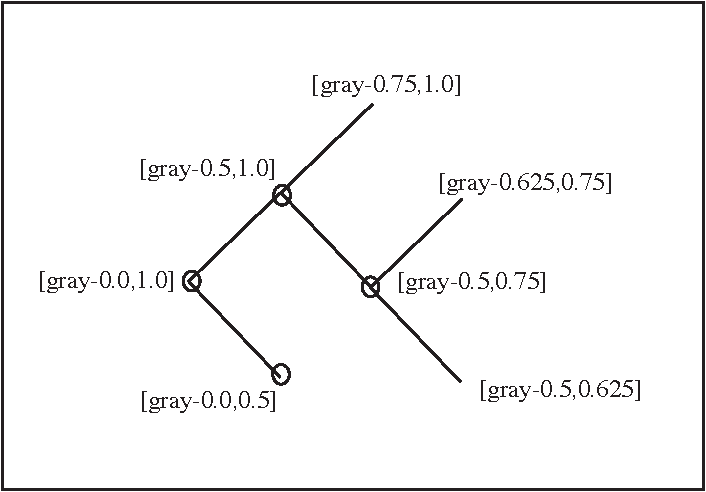
\includegraphics[width=.65\textwidth]{chap4/figs/tree}}
\caption{\label{trees} A discrimination tree contains
a set of categorizers which categorize by checking whether
a sensory value falls in the region of one category or 
not. The discrimination tree shown operates on
values on the GRAY channel.}
\end{figure}

As mentioned earlier, I will label categories
by using the sensory channel from which a category operates, 
followed by the minimum and maximum values of the region
carved out by the category. For example, 
[AREA 0.0-0.25] carves out the region [0.0,0.25] of the 
area channel. When it must be emphasised that 
a category belongs to a particular agent, for 
example {\bf a1}, I will write [AREA 0.0-0.25]$_{\bf a1}$. 

Conjunctive combinations of categories also have
dedicated categorizers which are linked to 
the categorizers of their components (see 
\figref{disnet}). A conjunctive combination 
often yields a more efficient way to pick out 
the topic compared to a single, possibly very fine-grained
distinction. For example, it might be that 
[AREA 0.0-0.25] {\it and} [GRAY 0.5-1.0]
together are distinctive but none of the two on their
own is. Other logical combinations are equally of interest
but I will restrict my attention to conjunctive 
combinations. Conjunctive combinations of categories 
will be written between curly brackets (\{,\}) as in 
\{[AREA 0.0-0.25] [GRAY 0.5-1.0]\}. 
\begin{figure}[htbp]
  \centerline{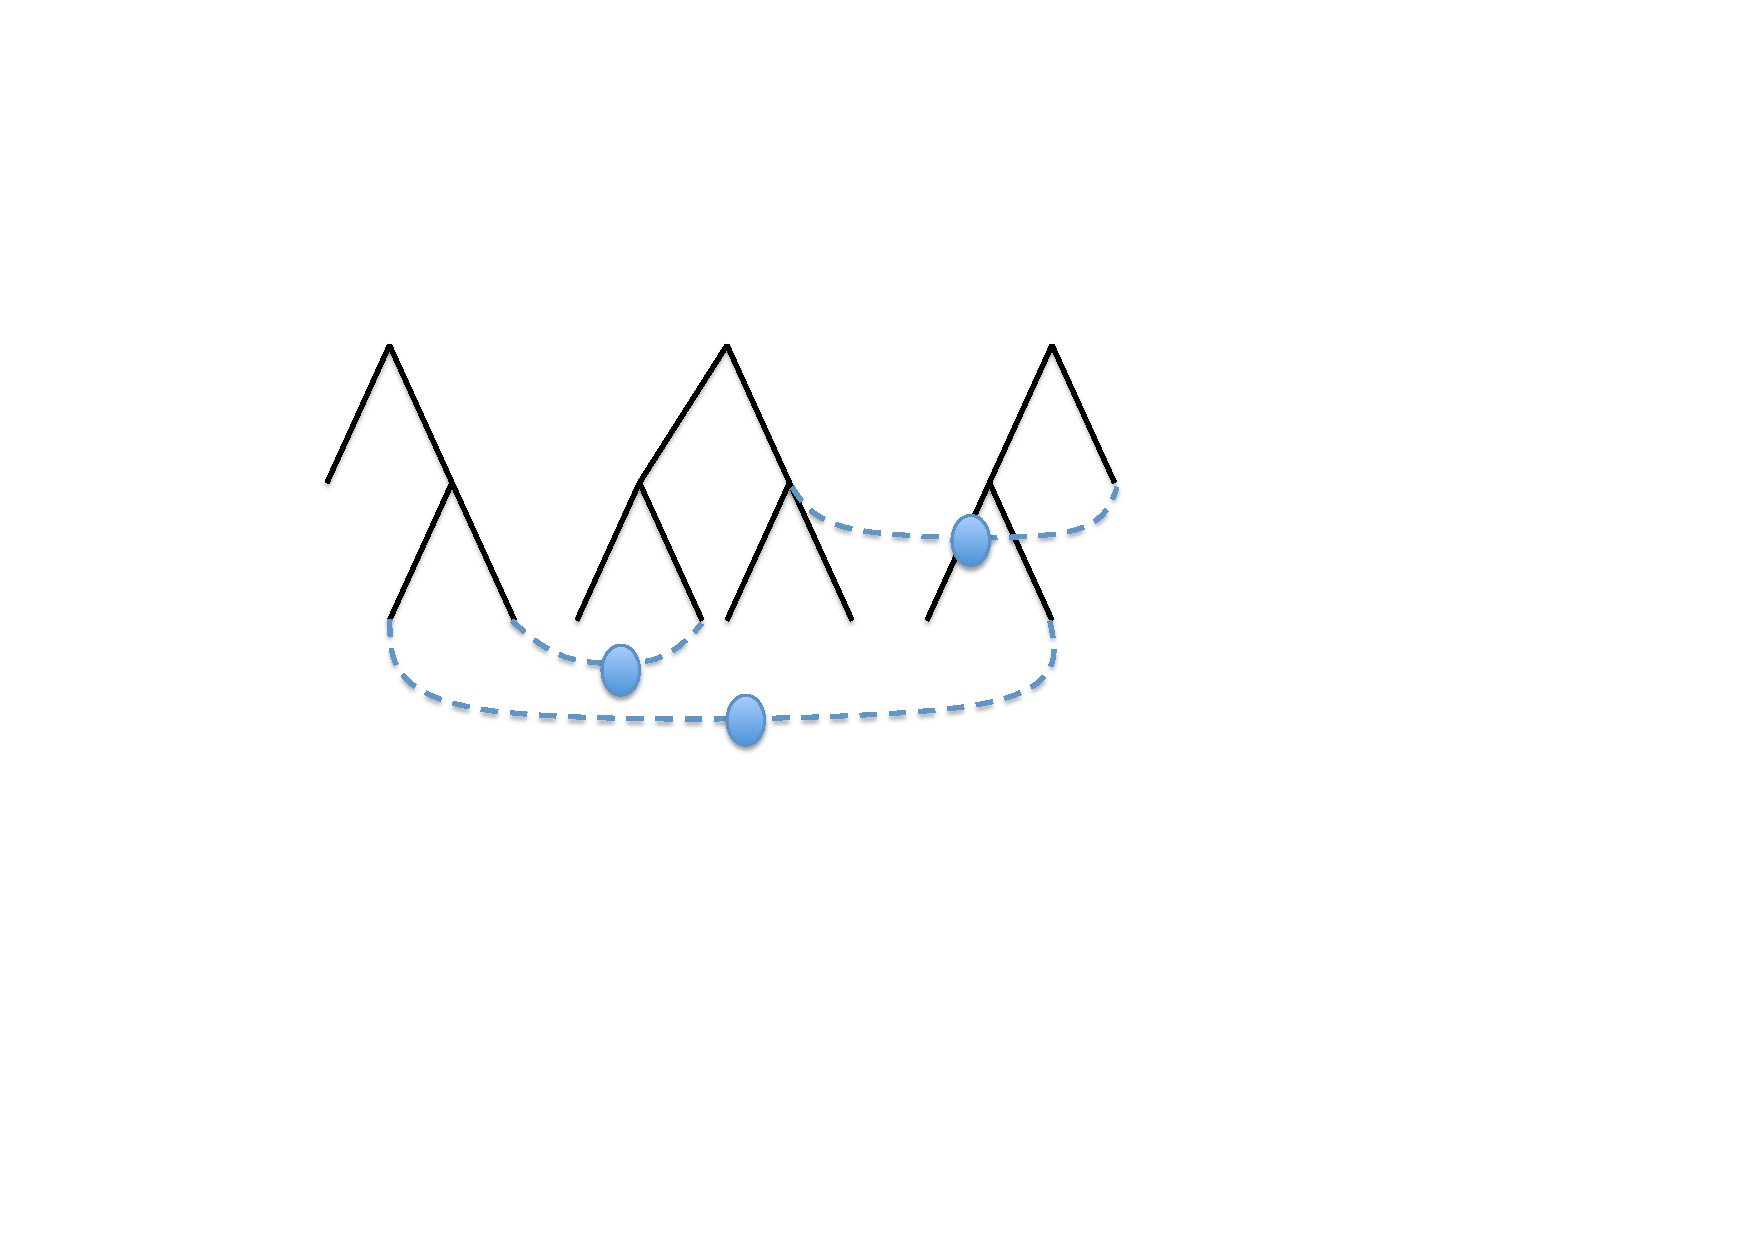
\includegraphics[width=.65\textwidth]{chap4/figs/disnet}}
\caption{\label{disnet} More complex categorizers
(shown as circles) are formed from the combination
of primitive categorizers.}
\end{figure}

\subsection{The discrimination game} 

\is{Discrimination Game}Here is a game, which I call the discrimination game, which is useful 
to study categorization in 
a systematic way.\footnote{
The discrimination game model together with the 
discrimination trees and its growth dynamics 
was presented for the first time in \cite{Steels:1996}
Based on this paper a new implementation of
single category discrimination was implemented by Angus McIntyre 
within the BABEL environment. Later on, Joris Van Looveren
re-implemented the use of conjunctive combinations.}
The game is played by a single agent, randomly 
drawn from a population of agents, and 
is equivalent to the conceptualisation phase of 
the guessing game. The agent perceives the scene and 
chooses a topic from the possible objects segmented in the
scene. He then uses his discrimination trees, as developed so
far, to come up with a category or a conjunction
of categories that is valid for the topic, but not for any
other object in the context. The discrimination game succeeds if 
the agent has found distinctive categories, otherwise the game
fails. When the game succeeds, the success counter
of the categorizers involved go up. 
\begin{figure}[htbp]
  \centerline{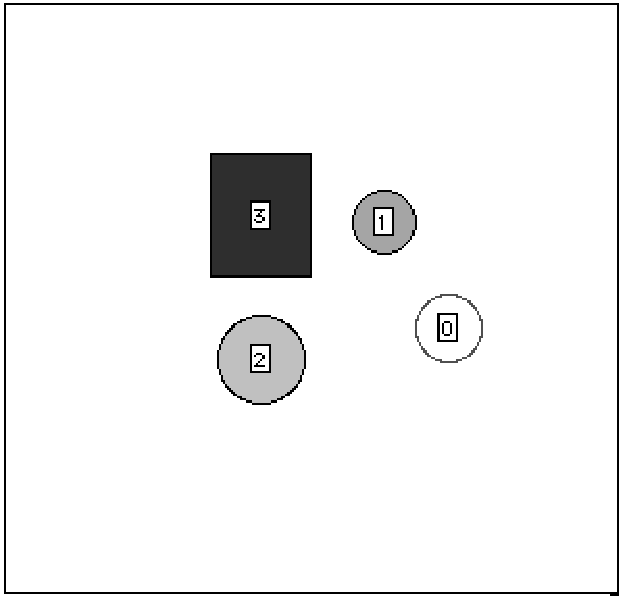
\includegraphics[width=.40\textwidth]{chap4/figs/game5}}
\caption{\footnotesize \label{geom} A computer generated scene 
from the GEOM world.}
\end{figure}

I will now develop some concrete examples, which imply
that I make choices for the kinds of sensory channels
and scenes that the agents use. 
I will first use scenes from the GEOM world as in 
\figref{geom} and later real world scenes captured
with a Talking Heads camera. 

Consider the scene in \figref{geom}. Assuming that the agent
already has a well-developed set of categories, he could use 
the category [GRAY-0.75,1.0] (very dark) to distinguish 
shape 3 from the others. On the other hand, if shape 2 is 
chosen as topic, the grayscale will not be enough because
shape 2 has the same grayscale as shape 1. Maybe a 
combination of categories can be chosen, like [VPOS 0.0-05]
(lower), and [HPOS 0.0-0.5] (left). Indeed shape 2
is lower in the scene, as opposed to
shape 1 and shape 3, and it is more to the left compared 
to shape 0 and 2.

\subsection{The Pachinko machine}

\is{Pachinko machine}Any visitor to Japan sooner or later comes across a 
Pachinko hall where eager players sit before a 
machine in which a metal ball, inserted at the top, 
falls through a series of gates until it falls in 
a winning or a losing bin. These games are
a possible metaphor to visualise the categorization process
based on discrimination trees. 

Imagine that for each object in
the scene and for each sensory channel, there is a ball
containing the value for that object on that channel. It
is introduced in the top categorizer of the 
discrimination tree associated with that channel. 
For example, suppose that there are three
objects in the scene: $O1$, $O2$, and $O3$, 
with gray-scale values 0.6, 0.4, and 0.9 respectively. 
We can therefore imagine three balls labeled with these datavalues
which are input to the top categorizer of the 
GRAY discrimination tree (\figref{balls}). 
A categorizer divides the balls in two bins, 
those that fall in the range of 
one category and those that fall into the range of the other
category. In this case, the left bin contains \{$O2$\} 
(category [GRAY 0.0-0.5]) 
and the right bin \{$O1$, $O3$\} (category [GRAY 0.5-1.0]). 
\begin{figure}[htbp]
  \centerline{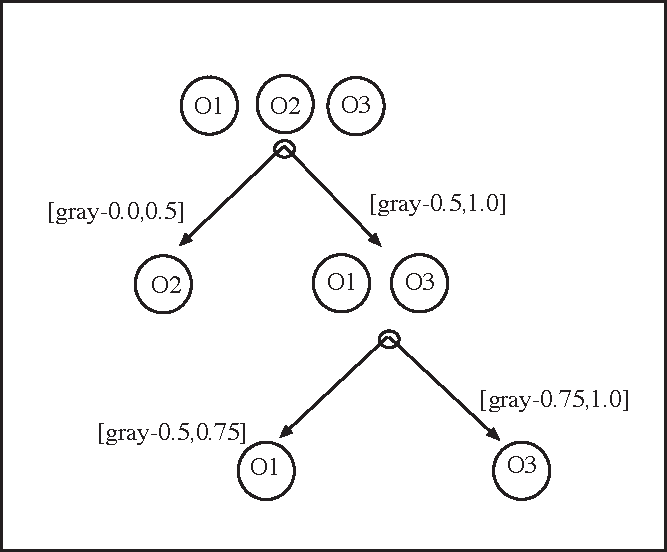
\includegraphics[width=.65\textwidth]{chap4/figs/balls}}
\caption{\footnotesize \label{balls} Balls containing
the data value for the different objects
$O1$, $O2$, $O3$ in the scene. $O1$ is the topic.
$O1$ has the value 0.6 on the GRAY-channel, $O2$ has
0.4 and $O3$ 0.9.} 
\end{figure}

A distinctive category is found when the ball of the 
topic is the only one left in one of the bins. 
If the topic is $O1$, then this is not yet the 
case, because it is together with $O3$ in the 
bin of [GRAY 0.5-1.0]. However when the next categorizer
is exercised, it splits the set \{$O1$, $O3$\} 
into two subsets: \{$O1$\} for [GRAY 0.5-0.75]
and \{$O3$\} for [GRAY-0.75,1.0]. 
[GRAY 0.5-0.75] is a discriminating category because only 
$O1$ is left in its bin. 

Balls thus trickle down from the top to the bottom of 
a discrimination tree, like in the Pachinko game or 
a lottery machine. The trickling down process can stop as
soon as a distinctive category is found because finer grained 
distinctions are not necessary. 

\subsection{Competition between categories}

A realistic agent has hundreds of sensory
channels, and humans probably have tens of thousands
of them, probably grouped with respect to the domains
to which they apply.\footnote{
This is strongly suggested by psychological 
data on the presence of conceptual spaces in human 
categorization. See \cite{Gardenfors:1999}.} There are discrimination trees
for each of 
these channels or for combinations of them, and 
each can possibly yield a distinctive
category. The categorization process can therefore be
envisioned like a huge Pachinko hall, in which
balls are trickling down in parallel in hundreds or 
thousands of machines. It is highly 
likely that more than one solution is found
when there are a lot of trees, particularly 
if combinations of categories are allowed as well. 
So, an additional competitive process must 
take place to rank categories even 
though multiple solutions are offered to subsequent
verbalisation processes. We see therefore the same
characteristics as for the perceptual layer, and thus
the `sieve architecture' also 
applies for the conceptual layer (\figref{f:sieve}). 
 
There are many possible criteria for preferring 
one category over another, equally distinctive one. 
The first is based on 
simplicity. A single category is less complex than 
a combination of categories, and a more abstract category 
is preferred over a more specific one. 
The second criterion is based on success in earlier games. 
Each categorizer monitors how many
times it was used and how many times
it was successful, i.e. how many times it could distinguish
the topic and participate in a successful language game. 
Another criterion, that I will bring in later 
once I have introduced the lexical layer, refers to 
success of the lexicalisations of the category. The agent 
will prefer categories where it is known that there is
a well-accepted way to express it. 
When ranking categories, these criteria are combined
and the best ones enter with the most force in the 
lexicalisation layer. 

Notice the hidden positive feedback effect\is{positive feedback} between success
and use: A categorizer which has already achieved
a higher score wins the competition, everything else being
equal, causing its score to increase even more. 
This way a consistent behavior emerges where the 
same category tends to be used in the same circumstances, 
similar to the way a walking path sometimes 
emerges for crossing a patch of grass between buildings. 
Initially many paths are possible, but once one path 
is used a bit more than others, it gets used more and 
more, as people reuse a path they perceive to be
there. I will show later (chapter 6) that this entrenchment of 
a particular solution by a positive feedback loop can 
be exploited through the structural coupling between 
the ontology (the set of categories) and the lexicon
(the set of form-meaning pairs verbalising categories), 
so that they become co-ordinated without a central 
co-ordinator.\footnote{
I adopt here other general principles of complex
systems. The notion of structural coupling has been 
introduced by \cite{Maturana:1992} and is 
now widely used to explain various forms of 
biological co-ordination.}

\subsection{Variations on discrimination}

There are obviously many variations on categorization
that could be imagined. For example, a categorizer
could make use of focal points instead of regions. A focal 
point is a single significant data value of a sensory channel.
The categorizer then has to compute the distance 
between the value for a segment and the focal point 
of each possible category. The category 
whose focal point is closest to the sensory value
of a segment applies. This implements a `prototype-like'
approach to categorization which has been argued to 
be more realistic with respect to human categorization.\footnote{
See \cite{Varela:1991} and \cite{Taylor:1989}.}
For example, humans typically label light
at 482 nanometer as the most typical blue, so that a given object
reflecting light at or near this point is categorized
as [BLUE]. Categories based on focal points are 
interesting and have clear advantages 
but I will stick nevertheless in the first instance 
to binary discrimination trees operating on single sensory 
channels to simplify the explanations
and to analyse better what is going on. 

Still another way to categorize reality is by imposing 
an order on the segments based on their values for 
a particular sensory channel. For example, we can 
order the segments based on the HPOS channel (i.e. 
from left to right) and then introduce relational categories
like `left of one segment in the series', or `the left-most object'. 
Similarly we can order the segments based on the 
HEIGHT channel (i.e. in terms of their size) and then 
have categories that select the smallest (i.e. the 
first segment in this ordering), or those greater than 
some other one. 

Of course, I am well aware that this categorization 
process captures only the most basic way of generating
meaning. Human beings make extended use of metaphor, 
analogy, metonymy, and other processes that adapt 
conceptual structures from one domain to another one.\footnote{
See: \cite{Johnson:1987}.}
But before we can study such processes we must understand
how basic perceptually grounded categories can 
originate. 
 
\subsection{The Discrimination Game in action}

Let us now look at some example 
games for an agent {\bf a1} taken from simulations
using computer generated
scenes from the GEOM world and showing the internal
structures generated as well as the reports from the commentator. 
At first I will not take saliency nor 
context-scaling into account. The first game
(game 8) fails. It takes place near the very beginning 
when {\bf a1} has practically 
no repertoire of distinctions yet. The scene and the 
discrimination trees available so far are shown in Figure 
\ref{scene2}. The object labeled 0 is the
topic. Only two channels have top level
categorizers: HEIGHT and WIDTH. 
The data on these channels for the scene in Figure
\ref{scene2} are shown in \tabref{tab:t-game8}. 
\begin{table}
\begin{center}
\begin{tabular}{ l  l  l }
\lsptoprule
{\it Object} & {\it HEIGHT} & {\it WIDTH} \\ \midrule
0 (square) & 0.413 & 0.317  \\ 
1 (circle) & 0.410 & 0.410 \\ 
2 (square) & 0.163 & 0.163 \\ 
\lspbottomrule
\end{tabular}
\caption{\label{tab:t-game8} Sensory data for the scene in \figref{scene2}.}
\end{center}
\end{table}

HEIGHT and WIDTH have been scaled with respect to the 
minimum and maximum height and width of a 
figure (sensor-scaling) but no context-scaling has 
been performed. 
\begin{figure}[htbp]
  \centerline{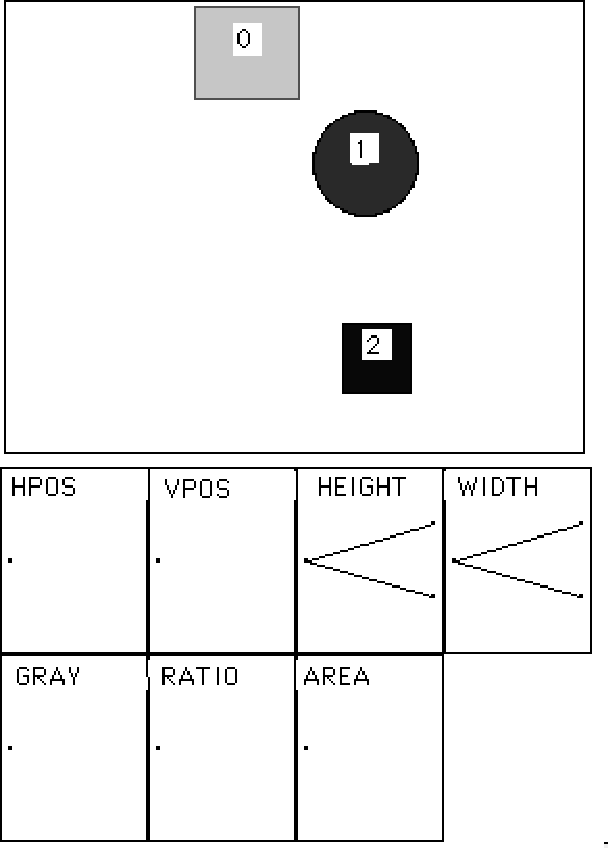
\includegraphics[width=.40\textwidth]{chap4/figs/scene8}}
\caption{\label{scene2} Top: The scene used in game 8. 
Shape 0 is the topic. Bottom: The discrimination trees available
for this game.}
\end{figure}
The game is reported by the commentator as follows: 
\begin{verbatim}
Game 8
 a1 segments the context in 3 objects: 
    square-0, circle-1, square-2
 a1 chooses square-0 as the topic
 The discrimination game fails
\end{verbatim}
The game fails because for the two sensory channels 
for which there are discrimination trees, the values 
of the segments are all within the lower range and so 
no distinctive category or category set could be found. 
This failure stimulates
the discrimination network to expand, but any node, 
including a top node of some of the other sensory channels 
can be chosen for further expansion. 

\begin{figure}[htbp]
  \centerline{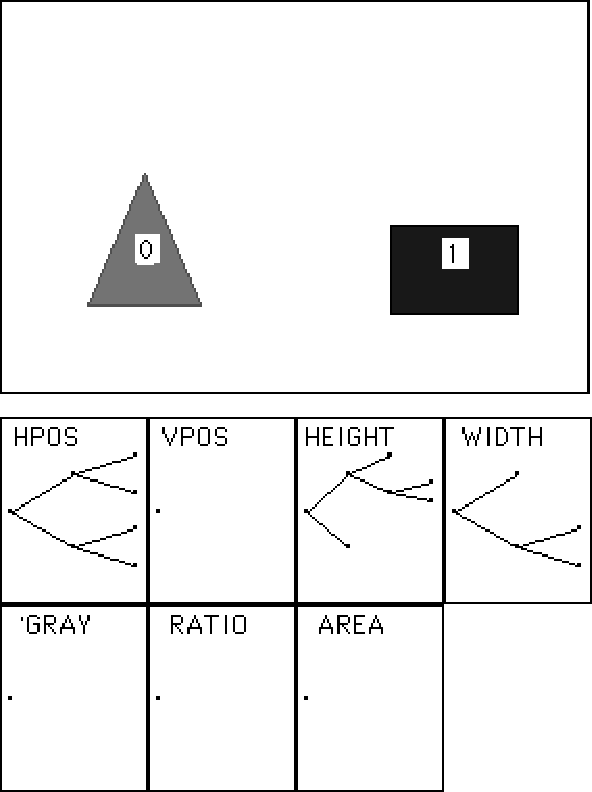
\includegraphics[width=.40\textwidth]{chap4/figs/scene22}}
\caption{\label{scene3} Top: The scene used in game 22. 
Bottom: The discrimination trees available to the
agent.}
\end{figure}
The next example shows a game (game 22) based on the scene 
in \figref{scene3}. The topic is the triangle, shape 0. 
The discrimination trees for 
HEIGHT and WIDTH have already more than one level and 
a discrimination tree for HPOS has developed.
The relevant sensor-scaled data for these three sensory
channels is shown in \tabref{tab:t-game22}. 
\begin{table}
\begin{center}
\begin{tabular}{ l  l  l  l }
\lsptoprule
{\it Object} & {\it HPOS} & {\it WIDTH} & {\it HEIGHT} \\ \midrule
0 (triangle) & 0.167 & 0.437 & 0.573  \\ 
1 (rectangle) & 0.789 & 0.563 & 0.287 \\  
\lspbottomrule
\end{tabular}
\caption{\label{tab:t-game22} Sensory data for the scene shown in \figref{scene3}.}
\end{center}
\end{table}

The scene is very simple so there are several possible
solutions: The triangle is more to the left, it is less wide 
and taller. Each of these possibilities is discovered
and their score (purely based on past performance) is 
looked up. The game is reported by the commentator
as follows: 
\begin{verbatim}
Game 22
 a1 segments the scene in 2 objects:  
   triangle-0, rectangle-1
 a1 chooses triangle-0 as the topic 
 a1 categorizes the topic as [HPOS 0.0-0.5] (score 0.57), 
   [HEIGHT 0.5-1.0] (score 0.09), or 
   [WIDTH 0.0-0.5] (score 0.0) 
 The discrimination game succeeds
\end{verbatim}

\subsection{The importance of scaling and saliency}

The example of game 22 shows at once why context-scaling 
and saliency is important. When we inspect the scene in 
\figref{scene3}, we do not quite see so clearly 
that the triangle is less wide than the square, so why
is [WIDTH 0.0-0.5] 
nevertheless considered? Examination of the data shows
that the WIDTH values, 0.437 for the triangle
and 0.563 for the square, are very close 
to each other, but just by luck fall within 
the two regions carved out by the WIDTH discrimination
tree. On the other hand, the values on the HPOS channel 
are much further apart and so they are preferred. 

As we have seen in the previous chapter, 
saliency is the smallest of the absolute values     
of the distance between the topic and any
other object. It gives us an indication why 
a certain sensory channel should be preferred
over another. For the scene in game 22, the saliency for each channel with 
respect to the triangle is as in \tabref{tab:t-game22-sal}: 
\begin{table}
\begin{center}
\begin{tabular}{ l  l  l }
\lsptoprule
{\it HPOS} & {\it WIDTH} & {\it HEIGHT} \\ \midrule
 0.622 & 0.125 & 0.286  \\ 
\lspbottomrule
\end{tabular}
\caption{\label{tab:t-game22-sal} Sensory data for the scene in game 22.}
\end{center}
\end{table}
From this table we see immediately that HPOS is the 
most salient channel and should be preferred by far, followed
by HEIGHT and then WIDTH. Thus we can expect the
agent to choose HPOS based on saliency. When the saliency threshold
is set to a reasonably high value, the other channels
would not even be considered, they would not pass the 
sieve of the perceptual layer. 

The sensory channel data for the 
same scene now scaled for context is shown in \ref{tab:t-game22scaled}. Such context-scaling 
pulls the data further apart and makes categorization 
therefore much easier and much more 
stable, but the information on saliency is lost and so 
it is no longer clear which channel is to be preferred
for reasons of saliency. 
\begin{table}
\begin{center}
\begin{tabular}{ l  l  l  l }
\lsptoprule
{\it Object} & {\it HPOS} & {\it WIDTH} & {\it HEIGHT} \\ \midrule
0 (triangle) & 0.0 & 0.0 & 1.0  \\ 
1 (rectangle) & 1.0 & 1.0 & 0.0 \\  
\lspbottomrule
\end{tabular}
\caption{\label{tab:t-game22scaled} Sensory data for the scene shown in \figref{scene3}.}
\end{center}
\end{table}
So the best thing to do (and this is what the Talking Heads 
effectively do) is to first perform sensor-scaling, then 
compute saliency to determine which channel should be 
preferred, then perform context-scaling, to get clearly 
distinguished sensory values, and then do categorization. 
Note that context-scaling has the same effect as using 
prototype-based categorization because the actual values 
are pulled towards extremes, and thus perceived as 
prototypes. Context-scaling is not always desirable. For example, 
in the case of colour categorization the actual channel
data should be maintained because here categorization 
takes place on the basis of actual values. 

\subsection{Combinations of categories}

The next game (game 24) is based on the scene in 
\figref{scene4}. The topic is triangle-0. 
The discrimination trees are the same as for
game 22. The game (based on sensor-scaled values)
succeeds with a conjunctive combination of two
categories: 
\begin{verbatim}
Game 24
 a1 segments the scene in 4 objects: 
   triangle-0, triangle-1, square-2, rectangle-3 
 a1 chooses triangle-0 as topic
 a1 categorizes the topic as {[HEIGHT 0.0-0.5] [WIDTH 0.5-1.0]}
 The discrimination game succeeds
\end{verbatim}
\begin{figure}[htbp]
  \centerline{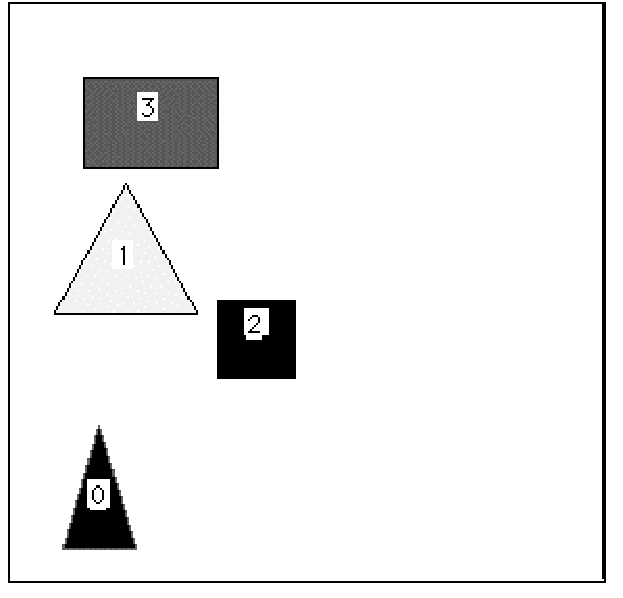
\includegraphics[width=.40\textwidth]{chap4/figs/game24}}
\caption{\label{scene4} The scene used in game 24.}
\end{figure}
The relevant data after sensor-scaling for the 
two sensory channels involved are shown in \tabref{tab:t-game24}. 
\begin{table}
\begin{center}
\begin{tabular}{ l  l  l  l }
\lsptoprule
{\it Object} & {\it HEIGHT} & {\it WIDTH} \\ \midrule
0 (triangle) & 0.170 & 0.513  \\ 
1 (triangle) & 0.653 & 0.570 \\  
2 (square) & 0.213 & 0.213 \\  
3 (rectangle) & 0.613 & 0.310 \\  
\lspbottomrule
\end{tabular}
\caption{\label{tab:t-game24} Sensory data for the scene in \figref{scene4}.}
\end{center}
\end{table}

[HEIGHT 0.0-0.5] is valid for triangle-0 and square-2 but
filters out the other segments. 
[WIDTH 0.5-1.0] is valid for triangle-0 and triangle-1 and 
filters out the others.  
The conjunctive combination of these two categories only 
retains triangle-0 and is therefore the one that is chosen. 

\subsection{A real world scene}

The next example is taken from a series of discrimination 
games played by physically instantiated agents using 
real world images. The series is discussed more extensively 
in chapter 7. The agent {\bf a2} has 
captured the image shown in \figref{f:plate-10}
(top left) and done the necessary segmentation and 
gathering of sensory characteristics. The resulting sensory
values (after sensor-scaling) for the segments are shown
in \tabref{tab:t-real}. Object-0 has been selected as the topic. 
\begin{table}
\begin{center}
\begin{tabular}{ l  l  l  l }
\lsptoprule
{\it channel}& {\it obj-0} & {\it obj-1} & Saliency\\ \midrule
HPOS & 0.27 & 0.16 & 0.11\\ 
VPOS & 0.20 & 0.20 & 0.0\\ 
HEIGHT & 0.15 & 0.15 & 0.0\\ 
WIDTH & 0.10 & 0.11 & 0.01\\ 
AREA & 0.10 & 0.10 & 0.0\\ 
R & 0.23 & 0.25 & 0.02\\ 
G & 0.32 & 0.34  & 0.02\\ 
B & 0.63 & 0.65 & 0.02\\ 
\lspbottomrule
\end{tabular}
\caption{\label{tab:t-real} Sensory data from a real world scene with segmentation shown in \ref{f:plate-10}.}
\end{center}
\end{table}
Clearly HPOS is the most salient channel and should be 
prefered by the agent. When performing context scaling, 
the two values for HPOS are drawn apart with 1.0 for object-0 and 
0.0 for object-1 so that the category [HPOS 0.5-1.0] (to the 
right) easily distinguishes the topic (object-0) from
object-1. The game is reported as follows: 
\begin{verbatim}
Game 3 
  a2 is the speaker. a1 is the hearer. 
  a2 segments the context into 2 objects: 
       object-0 object-1
  a2 chooses object-0 as the topic 
  a2 categorizes the topic as [HPOS 0.5-1.0]
\end{verbatim}
This example illustrates well why the categorization 
of the Talking Heads is so robust and why agents 
often share the same conceptualisation even if the details  
of their raw perception is quite different. 
The saliency factor helps to focus the agents on those
aspects of the scene that stand out. There is 
an enormous reduction of variation, first by scaling then by 
the categorization process itself. 

\section{An ecology of distinctions}

The previous section introduced mechanisms that 
enable agents to find a distinctive category or
conjunctive combination of categories given 
a set of segments and data on a series of sensory 
channels for each segment. I will now focus on the 
issue how discrimination networks and hence
repertoires of possible categories may develop. 

\subsection{Growth dynamics}

The process of growing categorizers is relatively
straightforward. In the very beginning, the agent
constructs top level categorizers for each channel which 
have contained at least once 
in the recent past relevant and distinctive
data. If a channel has the same data for every 
possible segment it is obviously not going to be 
possible to find a distinctive category no matter
how hard the agent tries. 

A new subcategorizer is constructed by taking a
categorizer node in the tree and dividing its range into 
two new subranges and thus two new subcategorizers.
For example, if there is a 
categorizer [HPOS 0.0-0.5], which triggers when the 
object is in the left most half of a scene, i.e. with HPOS
within $[0.0,0.5]$, then two 
subcategories are created by dividing $[0.0,0.5]$
into two halves, one for the 
range $[0.0,0.25]$ ([HPOS 0.0-0.25] or totally left) 
and one for the range $[0.25,0.5]$ ([HPOS 0.25-0.5] or mid-left). 
A new categorizer is added to the tree for each of these
halves. 

A categorizer based on a combination of categories is 
constructed by combining existing categories into a new one. 
Of course, if done without limits, this could create potentially 
a combinatorial explosion of possibilities. In the 
current implementation, the construction of combinations
is restricted by combining only those categories that 
have been partially successful in a given scene, 
just as only categories that
have ever been relevant are expanded. 

There are two key parameters to the growth process: 
(1) which category should be expanded and (2) when should
growth take place. In the Talking Heads experiment, agents expand 
a category which was effectively applied in the 
recent past, even though it may have failed in the game. 
This way the network is more likely to 
develop branches that are potentially relevant, although 
there is still no guarantee that the expansion
gives the distinctions required for the case at hand, 
because it is not based on an in-depth analysis of 
the case. 

Growth rate is proportional to failure. The more failures 
occur, the higher the likelihood of more nodes growing. This has the 
net effect of many new nodes growing in the beginning because
there are many failures, but that the repertoire of
categories stabilises
once discriminatory success is steady. When the environment 
starts to change again, causing new failures, more active 
growth is automatically triggered, which may lead 
to a renewed expansion of the repertoire. 

\subsection{Pruning dynamics}

Growth needs to be balanced by pruning. Pruning simply means
that a categorizer and thus its pending branches is 
cut away. There are again two
issues: (1) which nodes should be pruned and
(2) when pruning should take place. 
Obviously the score of a category should play a role
in deciding whether it should be pruned. 
categorizers that have not been used very much or have a low
success rate are prime candidates for removal, unless
any of their subcategorizers has a high score. The 
monitoring of use and success already played a role in 
determining which category should be prefered, so this
information is available to decide on pruning as well. 

Whereas the growth rate is proportional to failure, the pruning
rate is made proportional to success, so that 
in the case of a high failure rate the new categorizers are given
time to improve their score or to grow refinements that may be 
successful. A new categorizer obviously should be given
a grace period to encounter enough cases to prove
its worth, otherwise it could be cut out too quickly. Categorizers 
therefore not only monitor their use and success but 
also their age. 

\subsection{Average discriminatory success and repertoire size}

\is{discriminatory success}The Discrimination Game is a dynamical system.\footnote{
The theory of complex dynamical systems, which is well 
developed in the natural sciences, provides the 
theoretical foundation for studying the Discrimination
Game. For a general introduction, see \cite{Peitgen:1992}. 
Applications of these techniques to study the origins
of complexity based on computer simulations 
can be found in the regular conferences on Artificial
Life, proceedings published by MIT Press, Cambridge Ma.} A repertoire of
categories emerges in an agent gradually as an attractor of the
growth and pruning dynamics coupled to 
the environment. If growth is strictly proportional to failure
and there is no pruning, a point attractor
is reached as soon as the repertoire
is adequate, i.e. as soon 
as the agent consistently has success
for all the possible cases it encountered. However, 
as soon as the environment or the sensory capabilities of 
the agent change, in other words when new types of 
figures appear or when new sensory channels become available
to the agent, we expect that the repertoire of categories starts
expanding again. This could be seen as an illustration  of the
assimilation-accomodation dynamics envisioned by Piaget. 

Let me introduce a few measures 
to test whether all this is really happening with the 
mechanisms introduced so far.
The first (crucial) measure monitors 
how well the agent is doing by tracking
the average success in the most recent $n$ discrimination games. 
\figref{avsuc} shows the outcome of this measure, for 
agent {\bf a1}, playing 500 discrimination games in a
simulation with scenes from the GEOM world. 
Success is averaged per 25 games. We see clearly that {\bf a1}
has become successful in discriminating randomly chosen topics
from a consecutive series of scenes. Success rapidly climbs and
reaches 100 \%, even though the scenes are randomly
generated combinations from a repertoire of figures
along continuously varying 
dimensions making for literally billions of possibilities. 
The Discrimination Game is successful because it does 
not try to detect invariants or commonalities between consecutive 
cases but focuses on finding what is distinctive between the topic 
and the other objects. This enables the agent to make
such a gigantic abstraction leap and to make it at an amazingly 
rapid speed. 
\begin{figure}[htbp]
  \centerline{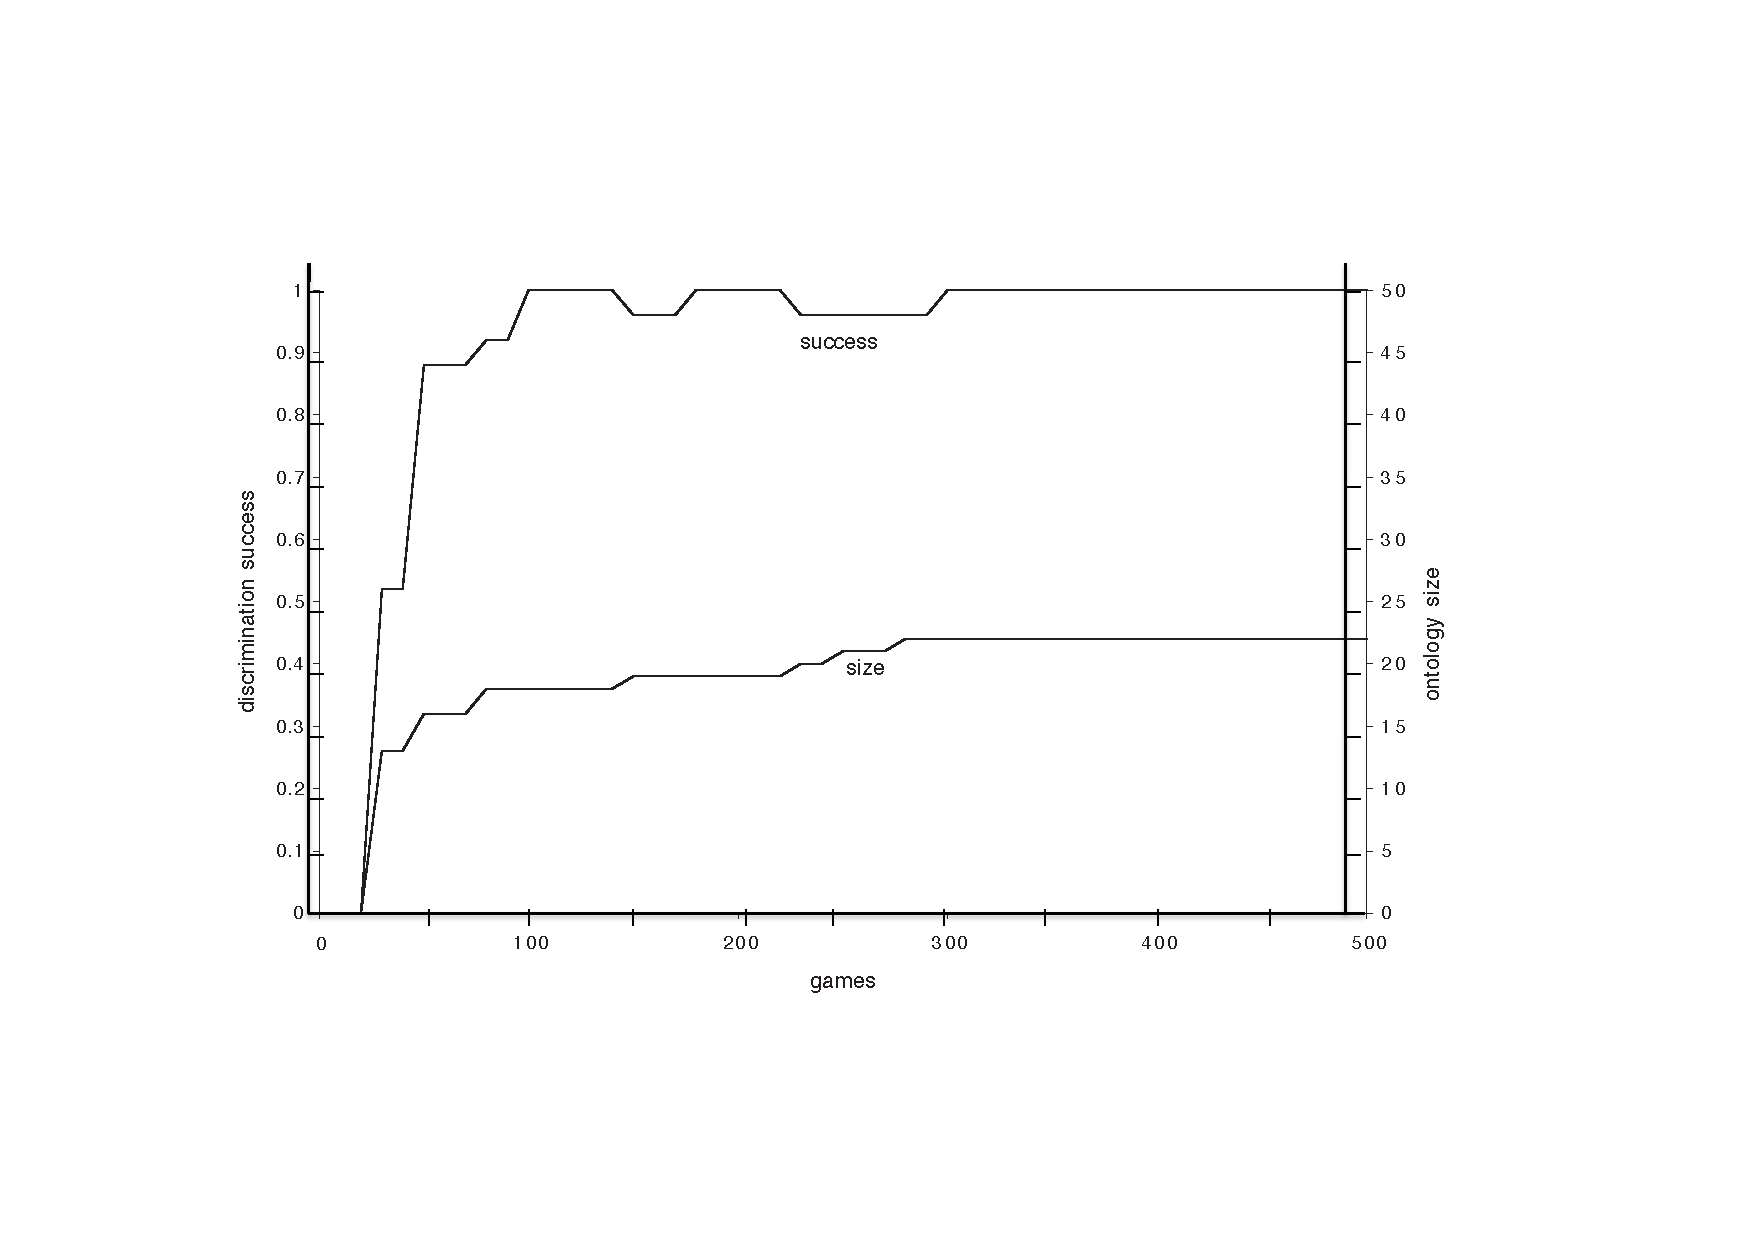
\includegraphics[width=.70\textwidth]{chap4/figs/avsuc}}
\caption{\label{avsuc} The graph displays the 
average success per 25 discrimination games for a
series of 500 games played by a single agent. Success climbs
to 100 \%. The graph also displays the size of the 
agent's repertoire of categories. Each scene contains
between 3 and 6 objects.}
\end{figure}

We can see whether a stable attractor has been reached by 
tracking the size of the repertoire, which is
simply the number of 
categorizers in the agent's discrimination trees. 
The result of this measure is also displayed in 
\figref{avsuc}. Once success is steady, the
size of the repertoire remains 
constant, which means that no new 
elementary distinctions arise nor do any distinctions
disappear. This is because there has been no pruning yet and 
growth is strictly proportional to failure. 

\figref{dyna-trees} shows some snapshots of the 
evolution in the discrimination trees of {\bf a1} as
the simulation continues and as additional situations
arise. There are
expansions, contractions, and shifts in the constitution of the 
discrimination trees but gradually there are fewer and 
fewer changes (compare for example (c) and (d)) as a
stable core emerges. 
\begin{figure}[htbp]
  \centerline{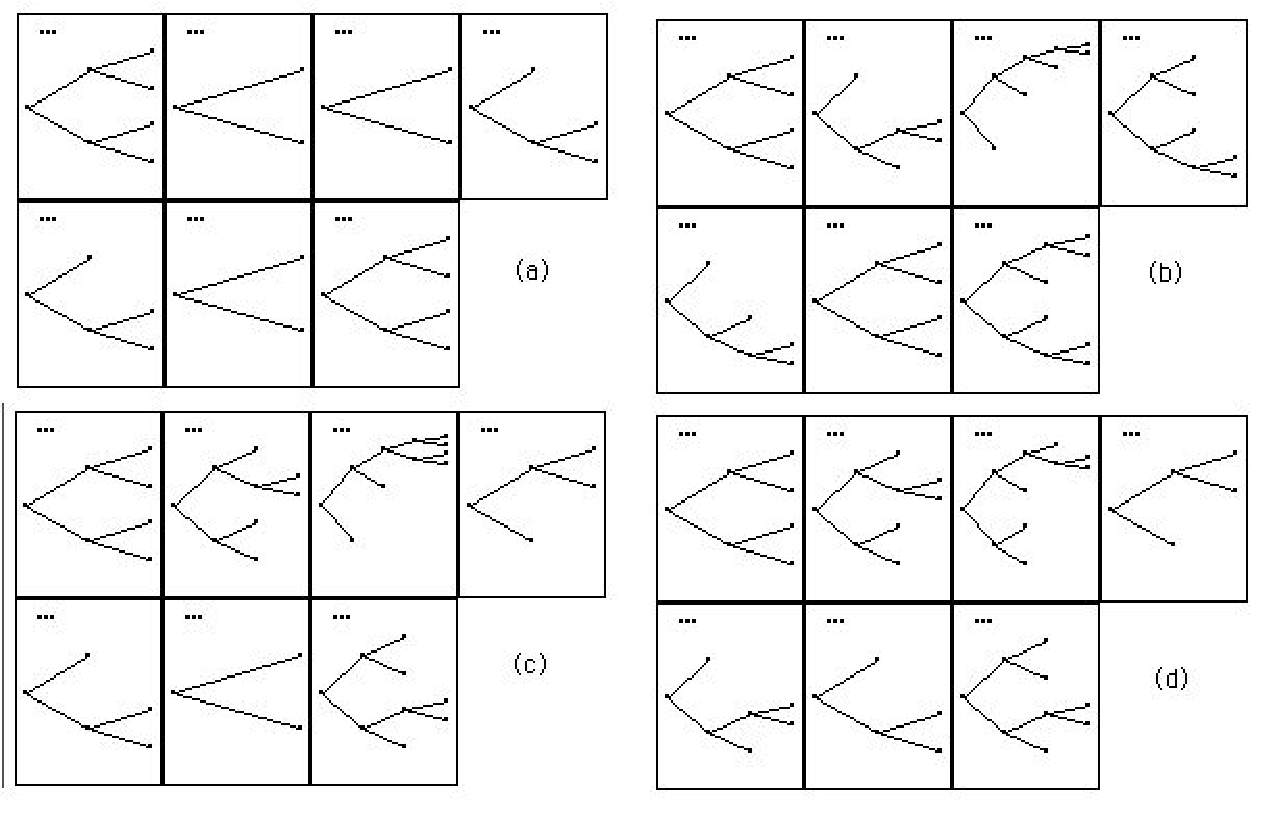
\includegraphics[width=.75\textwidth]{chap4/figs/dynatrees}}
\caption{\label{dyna-trees} Some snapshots of an evolving 
repertoire in a single agent using growth and pruning. 
Trees are shown after 500 games (a), 1000 games (b), 1500 games
(c) and 2000 games (d).} 
\end{figure}

These simulations show that the
category formation process based on a growth and pruning
dynamics is capable of creating a repertoire of
discrimination trees adequate for distinguishing 
the topic from other objects in the scene. The simulations 
worked with computer-generated, stylised environments
so that it is possible to probe the behavior of 
the mechanisms and vary the complexity of the environment. 
Note that the mechanisms are neutral with respect 
to the type of channels supplied. The discrimination 
trees and growth and pruning dynamics can operate over
auditory or bodily sensory channels, or other kinds
of visual information that is produced by low level 
perception. 

\subsection{Adaptivity in categorization}

\is{categorial adaptivity}An agent operating in a real world environment is always
going to be confronted with situations that he has 
not seen before. The growth and pruning dynamics of the 
discrimination game is capable of dealing with this because 
new distinctions grow when the failure rate 
is increasing. Here are the results of a computer 
simulation based on scenes generated by the 
GEOM world that test whether this is indeed the case. 

The simulation starts with a new virgin agent 
playing a series of discrimination games involving scenes
which only contain rectangles of the same graylevel. 
The agent has only channels for HEIGHT (0), WIDTH (1), 
RATIO (between the actual area of the shape 
and the area of the bounding box),
(2), GRAY (3) and AREA (4). We expect
to see that the discrimination trees on the RATIO (channel 
2) and GRAY channels (channel 3) do not develop because 
the values on those channels 
are the same for all objects ever seen. This is 
clearly confirmed in \figref{adptwrl1}: The ratio
between actual area and bounding box area is always 1.0
in the case of rectangles and they always have the same
grayscale value. 
We see clearly that the RATIO (channel 2) and GRAY (channel 3) 
do not develop and that the others develop to very 
fine levels of detail to still successfully discriminate. 
So discrimination trees only 
develop as needed in a particular environment, which is 
important for applying the selectionist
principle to the generation of sensory channels. 
The categorization process gives feedback to 
the sensory processing on the adequacy of particular sensory 
channels. 
\begin{figure}[htbp]
  \centerline{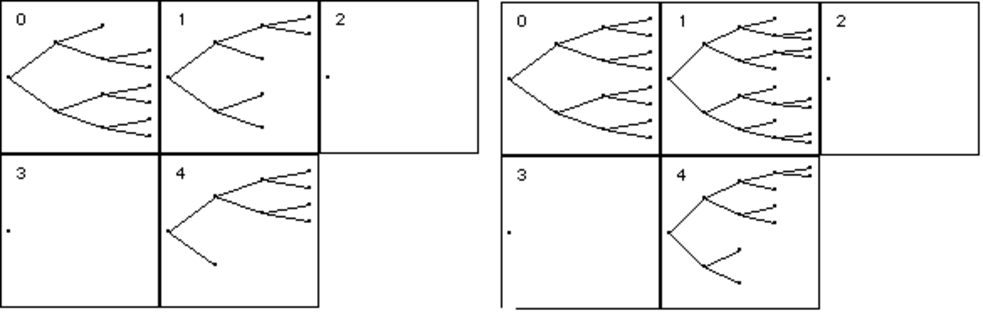
\includegraphics[width=.65\textwidth]{chap4/figs/adptwrl1}}
\caption{\label{adptwrl1} Two snapshots 
from a series of 500 discrimination 
games developing categories to distinguish rectangles of 
the same average graylevel. Channel 2 (the ratio channel) 
and channel 3 (the grayscale channel) do not develop.}
\end{figure}

Let us now make the environment richer by letting the 
GEOM world also produce scenes with circles and triangles, 
as well as rectangles. If the discrimination 
process is adaptive, the RATIO and GRAY channels should
start to expand because these channels now contain
significant data. This is indeed the case as shown 
in \figref{adptwrl2}. 
\begin{figure}[htbp]
  \centerline{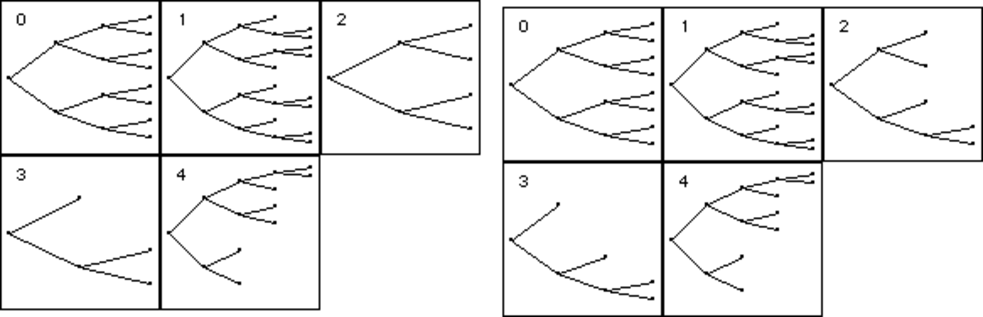
\includegraphics[width=.65\textwidth]{chap4/figs/adptwrl2}}
\caption{\label{adptwrl2} Two snapshots from 
an additional series of 500 discrimination games after
the environment has become more complex. RATIO
(channel 2) and GRAY (channel 3) have started to develop.}
\end{figure}

The simulation demonstrates
that the proposed discrimination process is adaptive to
changes in the environment, because growth picks up
as soon as the environment poses new challenges, just 
like the immune system starts generating a larger 
repertoire (and expanding already existing antibodies
that partially matched)
when challenged by the invastion of foreign bodies. 
The adaptation can be tracked with the success and 
repertoire size measures introduced earlier. 
When these measures are collected for the above example
(see \figref{adptwrlglo}), phase one shows clearly that 
when only rectangles are present, a stable 
repertoire gradually develops and that the success rate reaches 100 \%
after about 500 games. In phase two, when other types of 
shapes have been introduced,
the discrimination trees begin to expand again, now exploiting the
RATIO and GRAY channels to cope with the new types of objects.
Existing categories will of course still be adequate for 
many cases. After 500 more games, a new equilibrium
is reached. Steady discrimination success is seen with an 
enlarged repertoire.
\begin{figure}[htbp]
  \centerline{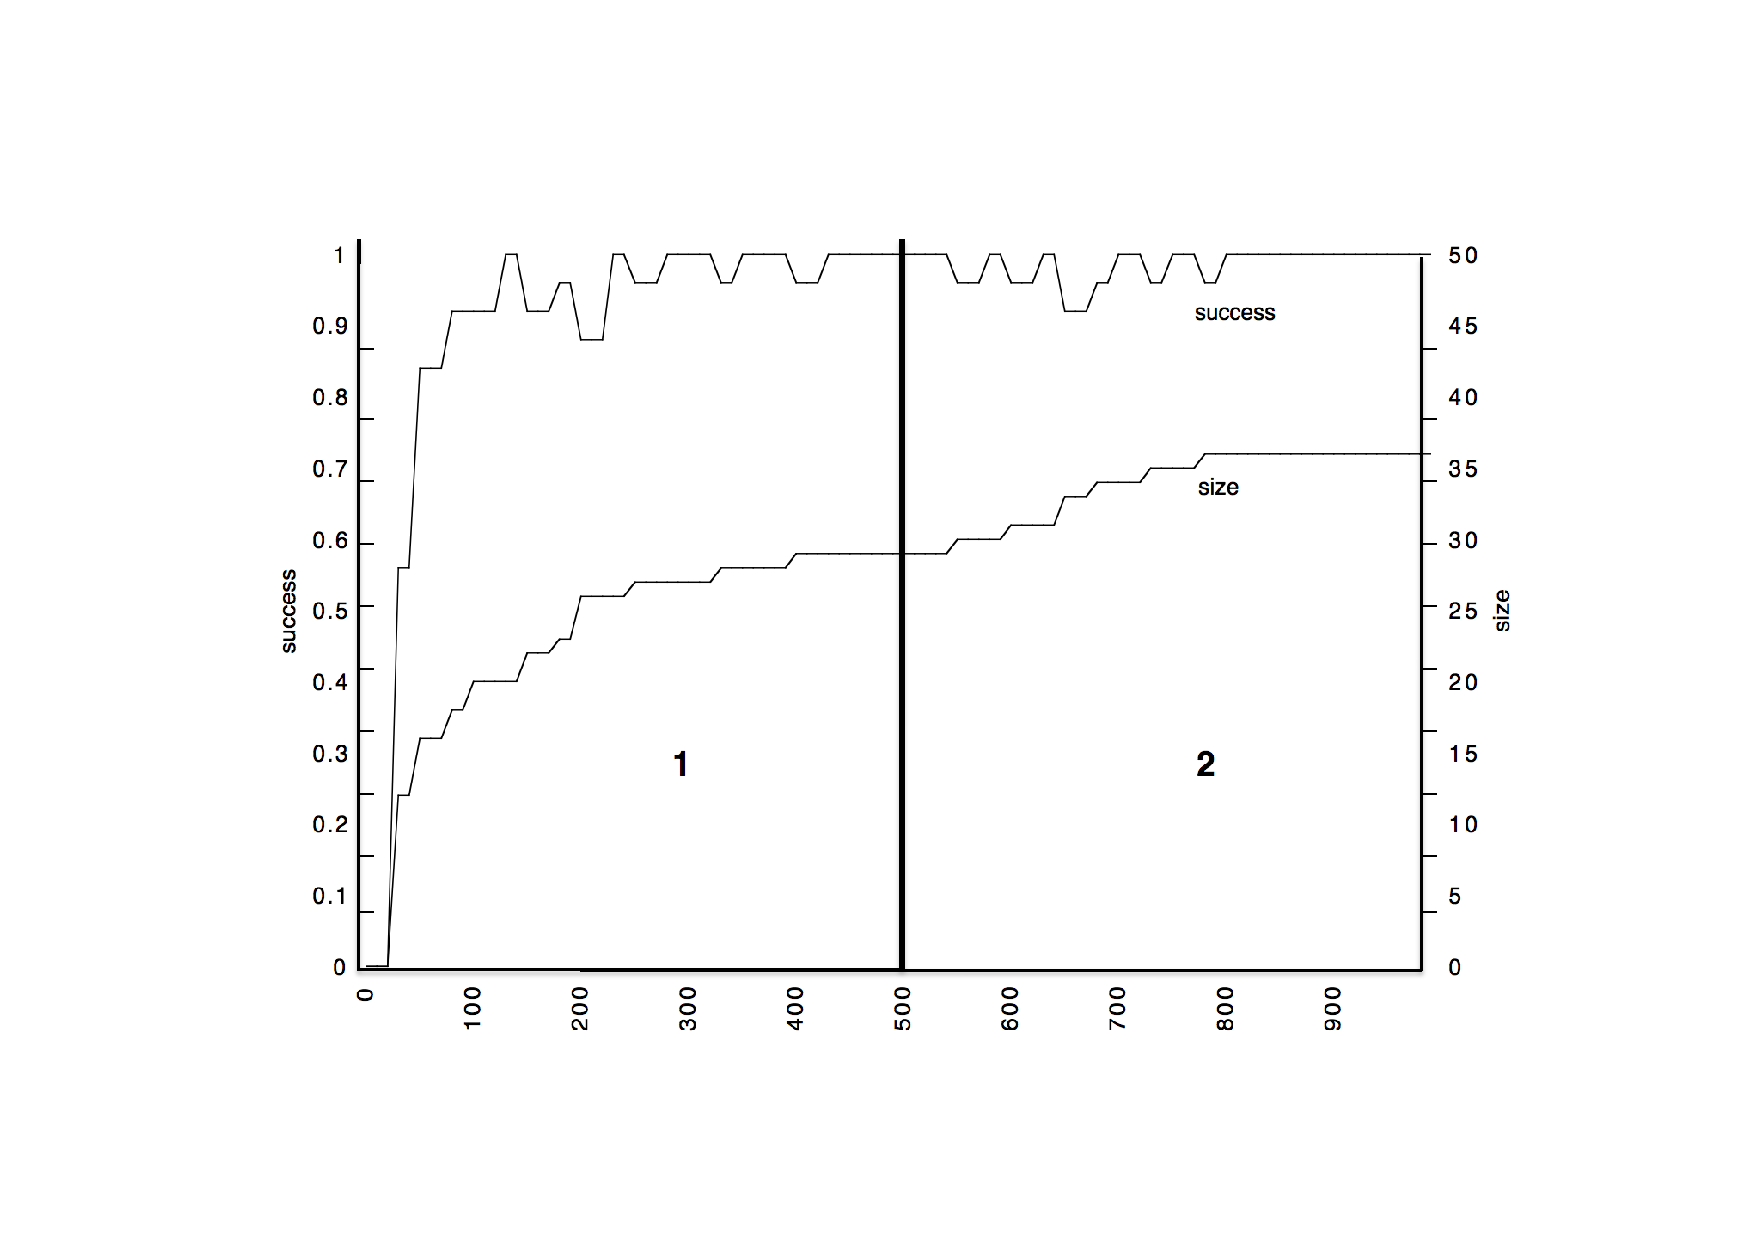
\includegraphics[width=.65\textwidth]{chap4/figs/adptwrlglo}}
\caption{\label{adptwrlglo} Evolution of success and ontology
size in a series of 1000 discrimination games played by a single agent.
In phase 1, only rectangles of the same graylevel are 
generated by the GEOM world. In phase 2, additional types of 
shapes are generated by the environment.}
\end{figure}

\subsection{Real world scenes}

Very similar developments can be seen when we do 
experiments with embodied agents, capturing real world scenes
through their cameras. \figref{discri200a} 
shows two snapshots of developing discrimination trees
for two agents. The game discussed earlier (based on 
plate 10, top) has been played with these trees. 
HPOS is the most salient channel and a distinction can 
be made easily. Note that the HEIGHT and WIDTH channels have not 
developed yet because no clear cases emerged 
in the environment where those channels provided 
salient data. 
\begin{figure}[htbp]
  \centerline{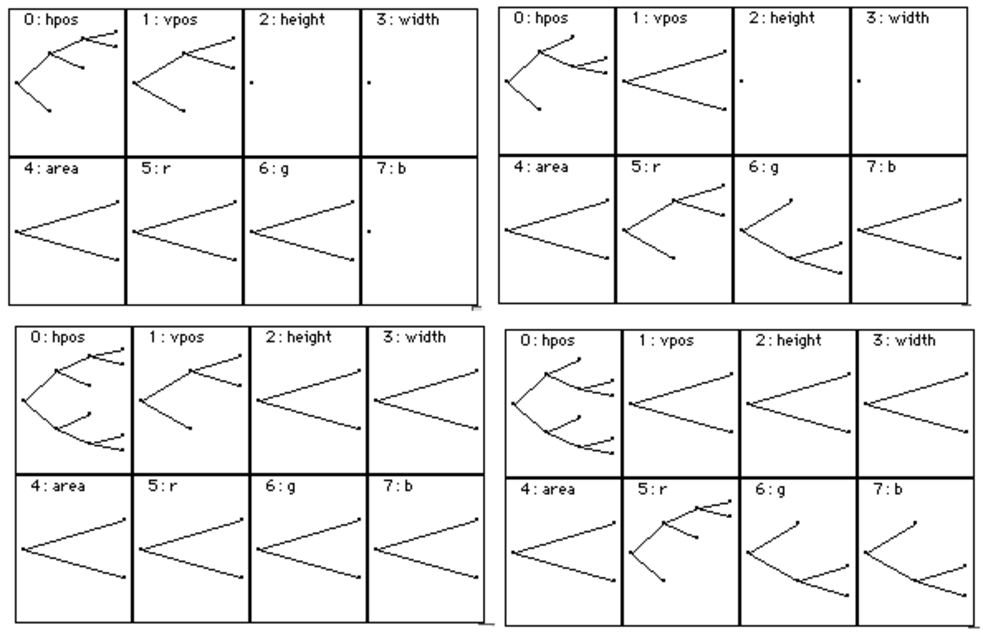
\includegraphics[width=.65\textwidth]{chap4/figs/discri200}}
\caption{\label{discri200a} The discrimination trees 
developed by two physically embodied agents 
{\bf a1} (left) and {\bf a2} (right). The top of the 
figure shows the trees after 
playing 100 games and bottom after 200 games.}
\end{figure}

\section{Conclusions}

This chapter addressed the problem of how agents may 
categorize their environment using information 
on sensory channels about each segment in the scene. 
I argued in favor of a selectionist approach, which 
generates possible solutions in a relatively 
random growth process and tests them in the 
cases presented by the environment. 
This approach contrasts with instructionism, where
the agent is assumed to make gradual abstraction 
from a series of examples using induction, and with 
a rationalist approach, where perceptually grounded categories are
assumed to be innate and hence derived through 
genetic evolution. 

The main conclusion of this chapter is that a selectionist
approach to the origins of categories
is theoretically and practically feasable. I have 
defined a growth and pruning dynamics which leads to 
an adequate repertoire for 
discriminating one object from the others in the 
same context and I showed that the repertoire is
continuously adapted when the environment changes. 

We will have plenty of opportunity in later chapters
to further test the mechanisms for categorization 
presented here. I will also introduce 
additional feedback couplings from the lexical 
layer to these categorization processes. Nevertheless
we are now sufficiently advanced to be able to
turn to the next subtask the agents face when 
engaging in a language game: establishing a relation
between categories or combinations of categories and 
an utterance. 

%There has been a long tradition of arguments for and 
%against a tight interaction between language and meaning, 
%exemplified with the debate triggered by the writings of 
%Whorf (See: \cite{Lee:1996} A recent survey of opinion and evidence
%can be found in: \cite{Gumperz:1996}.}


%\documentclass{../_combined/fcg-book}
\chapter{The Naming Game}

The semiotic square captures the four entities in 
a linguistic interaction: 
the {\itshape referent}, which is the object in the physical world that the 
speaker wants to communicate, the {\itshape segmented image}, which is 
the internal perception of the referent, the {\itshape meaning}, which is a 
category or combination of categories that picks out the 
referent in the present context, and 
the {\itshape utterance}, which is the word form 
or set of word forms transmitted by the speaker. In the previous 
chapters we looked at two sides of the semiotic
square. The relation between the real world and the
perceived image was studied in chapter 3 and the relation
between the perceived image and a conceptualisation that 
could act as the meaning for a language communication was 
studied in chapter 4. We now turn to the next side of 
the semiotic square: the relation between meaning and 
utterance. 

We need to find an architecture by which 
an agent can establish the relation between form and meaning, 
in other words verbalise a meaning to produce an utterance
and parse an utterance to retrieve its meaning. This 
mechanism needs to be flexible enough to deal with the 
unavoidable synonymy and amiguity that will arise. 
Second, we need to find a mechanism by which an agent 
can acquire and help construct the lexicon 
of the group. 
A shared lexicon should emerge
through the distributed activities of the agents without any prior
design or global co-ordination. Third, the lexicon formation 
process should scale up to handle a growing and ever
changing set of meanings and continue to work even with 
large populations whose constitution changes in time. 
It should be possible for new agents to enter the population
and acquire the existing language and for agents to 
leave without destabilising the whole system. These
are formidable challenges, particularly because we 
want to find the simplest possible solution, something 
a one year old child could do without fully 
developed intelligence. 

Immediately we observe a major difficulty. In realistic
language games, where agents cannot inspect each others' 
brain states nor transmit meanings directly, 
there is no feedback about the 
meaning of a word, only about the referent. For example, 
when a speaker says ``wabo'' and the hearer has correctly pointed 
to the referent that the speaker intended, neither the 
speaker nor the hearer can know whether they were 
using the same meaning. They can only know that they 
arrived at the same referent. When a game fails, the speaker 
can only point to the topic and the hearer then 
tries to figure out what possible meaning 
could have been applicable. The speaker cannot
communicate directly the `right' meaning, and very often more 
than one meaning is possible to distinguish a topic from 
other objects in the context, so that the hearer will 
not necessarily guess the meaning used by the speaker. 
I will call this the gavagai-problem, because Quine 
used this word to illustrate exactly this difficulty.\footnote{See \cite{Quine:1960}, p. 29,30.}
Quine evoked the problem of an anthropologist
trying to figure out what a native speaking an unknown
language might mean when he utters ``gavagai'' while pointing
to a white rabbit scurrying by. 

In this chapter, I will bypass the gavagai-problem by assuming
that agents get direct feedback about the meaning of a word. 
This is done by assuming that all agents share the 
same perception, that they already have
a repertoire of shared meanings, that for every agent
a particular meaning always picks out a single referent, and 
that a given referent is conceptualised with the same meaning 
by every agent. This scaffold allows us to focus on the problem
of how form-meaning associations might form and propagate in
a population without worrying how agents get feedback about 
the meanings of forms. However, it does means that we cannot 
do experiments with embodied physical agents but will have
to accept the limitation of working only
with computer simulations. 
The next chapter will take the scaffold 
away, as any serious theory for word meaning 
acquisition should. I will then show that given an 
appropriate coupling between lexicalisation and categorization, 
a communication system can still get off the ground based on 
the mechanisms described in this chapter. 

\section{Inventing a lexicon}

\is{Naming Game}I will now introduce another game, the Naming
Game, to allow us to focus on the origin of the lexicon.
The Naming Game defines a situation requiring 
a group of distributed autonomous agents to develop and 
use a shared lexicon relating forms and meanings, 
assuming they have a shared repertoire of meanings and get 
direct feedback about what meaning corresponds to a
certain form. The Naming Game can be thought of 
as the lexical side of the Guessing Game.\footnote{
The Naming Game and associated computer simulations
were presented for the first time in \cite{Steels:1996a}.}
The game can be implemented with different
mechanisms compared to the ones I will use, so it defines a 
task setting in which different solutions can be compared. 
See also \cite{Hutchins:1995}.
A different task setting for studying language acquisition
(but not how a language may emerge from scratch) is 
illustrated in \cite{Regier:1996}. In this case, the agents
are shown examples and counter-examples together with 
words they should use in each case. 
\newline 
It can be objected
that the Naming Game (and the Guessing Game) already 
assumes that the agents want to communicate. 
This is true, but the game can be embedded in a larger
setting where communication is vital for survival. 
An example of such a setting is discussed in \cite{Werner:1991}. \newline
Another issue concerns
the evolution of the game itself. This topic is discussed in: 
\cite{Hurford:1989}. This paper is also
the earliest paper posing the problem of the origins of 
a lexicon through computational simulations. See also: 
\cite{Oliphant:1996}. \cite{Hauser:1996}
contains a further discussion of these topics from the 
viewpoint of biological continuity.

The Naming Game is played by two agents, a speaker and 
a hearer, which are picked randomly from a population. 
The speaker selects a meaning from the shared repertoire
of meanings, looks up a possible word for this meaning 
in his lexicon, and transmits the word to the hearer. 
The hearer interprets the word by looking it up in his lexicon, 
and transmits the meaning he thus obtained. If this meaning 
is the one that the speaker originally had in mind the 
game succeeds, otherwise the game fails. When the game 
fails, the speaker communicates the meaning directly so 
that the hearer can acquire a new form-meaning pair 
for later conversations. When a speaker does not have a
word yet for a meaning he wants to communicate, he may create 
a new one. 

\subsection{Representing lexical associations}

What cognitive architecture do agents need to engage in naming 
games? Clearly they need some sort of {\itshape associative memory} to\is{lexical memory}
store their individual lexicons.
Let us assume that agents 
can construct and recognise arbitrary consonant-vowel combinations, 
like ``coba'' or ``wabidu'', for forming words, and that they 
have a repertoire of possible meanings in the form of 
categories, for example [LEFT], [DARK], [LARGE], etc. 
The contents of the associative memory of a single agent can
be displayed in a table as follows: 

\begin{table}
\begin{center}
\begin{tabular}{ l  l }
\lsptoprule
{\itshape meaning} & {\itshape form} \\ 
\midrule{}
{}[DARK] & coba \\ 
{}[LARGE] & wabidu \\ 
... & ... \\ 
\lspbottomrule
\end{tabular}
\end{center}
\caption{\label{tab:t-mem} Associative memory of a single agent.}
\end{table}
As an agent is acquiring his lexicon, there are going to 
be stages when he is not yet sure about the meaning of 
a certain form. So it must be possible for the agent
to store different 
meanings for the same form and different forms for the
same meaning. This can easily be done by extending the memory capacity
to cross-associate multiple items. Agents can then 
handle amiguity (one word can have different
meanings) and synonymy (one meaning can 
be associated with many different words). 

A speaker can only transmit a single choice for 
expressing the meaning.
When there are alternative words for the same meaning in 
his lexicon, he must decide which one to use and this decision
should be such that it maximises success in the game. 
To estimate this success, 
each agent should monitor for each form-meaning association
how successful it has been, which could be implemented 
by associating with every form-meaning pair 
a {\itshape score}.\is{score} The score of a form-meaning pair
is specific to an agent and based only on his own 
local interactions with other agents, in line with the 
principle that no single agent has a complete overview of 
the lexicon nor controls the others. An example of 
a lexicon with multiple associations and a score for every 
association is illustrated in \tabref{tab:mem2}. 

\begin{table}
\begin{center}
\begin{tabular}{c c c c  c  c  c } \lsptoprule 
& coba & zapo & bila & pama & wabidu & limiri \\ 
\midrule {}		
{}[DARK] & 0.3 & 0.2 & 0.1 & 0.8 & - & - \\ 
{}[LARGE] & - & - & - & 0.5 & 0.3 & 0.6 \\ 
\lspbottomrule
\end{tabular}
\caption{\label{tab:mem2} Example lexicon with multiple associations.}
\end{center}
\end{table}
From this table we see that the agent prefers to use the 
word ``pama'' for [DARK] and ``limiri'' for [LARGE]. 

\subsection{Updating the score}

One of the crucial aspects of the Naming Game model
is how scores are updated based on the outcome of 
a game. Intuitively 
the score should be related to use and success. 
The more a word is used and the more success it 
has, the higher the score should be. Moreover
there should be a time dimension, 
as recent use and success should obviously contribute
more to the current score. 
The following is a scheme that captures these
characteristics. 

Every time an agent successfully uses a form-meaning pair 
for speaking, he increments
the score with a specific increment $\delta$. 
$\delta$ is relatively high, typically equal to 0.1. 
The scores of competing associations, i.e. 
associations that used another form for the same meaning
are decremented with $\delta$. The score remains however bounded 
between 0.0 and 1.0. This way the `best' 
form-meaning pair stands out more clearly next time 
around.\footnote{A systematic investigation of alternatives for 
the updating function is contained in \cite{Oliphant:1997}. 
The dynamics of the mechanisms used in the 
Talking Heads experiments are being investigated in the
Ph.D thesis of Frederic Kaplan.}

When an agent plays the role of hearer, he also increments
the association that was successful with $\delta$, and 
decrements competing associations, i.e. associations that related
another meaning to the same form. When a 
game fails, the associations used by the speaker
and the hearer that contained the transmitted 
word form are both decremented. 

The operations of speaker and hearer are summarised in 
\figref{incr-decr} assuming that speaker and hearer
use both the score table above (in reality they of 
course always have different score tables). 
The speaker collects all possible
forms for a given meaning [DARK], chooses the one with the
highest score (``pama''), and transmits that form. 
The hearer collects all possible meanings for 
the transmitted form ([DARK], [LARGE]) and again chooses the one with
the highest score. If the hearer's meaning is equal to that
of the speaker's, the game succeeds. The score of 
two used associations increases and the others
decrease, implementing lateral 
inhibition. If the game fails, only the two used associations 
go down.\footnote{More or less neural realism can be introduced to 
model this associative memory. In our experiments we 
have a perfectly working memory that can store an 
association as soon as it has seen it once. This makes
theoretical investigation easier and makes it possible
to better follow the simulations and experimentations.  
An example of a neural network solution to lexical
memory is discussed in \cite{Cangelosi:1996}.}


\begin{figure}[htbp]
  \centerline{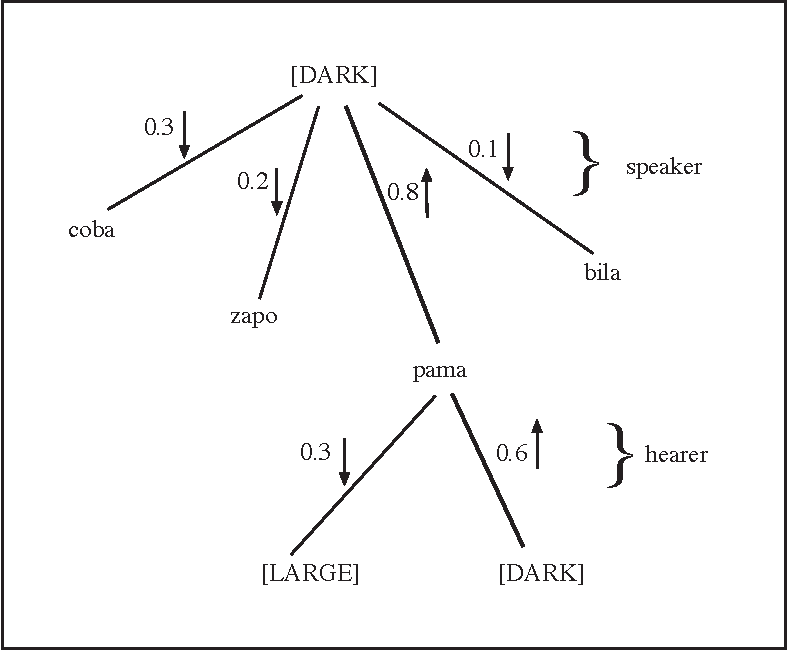
\includegraphics[width=.60\textwidth]{chap5/figs/incr-decr}}
\caption{ \label{incr-decr} 
Score adjustments after a successful game. Scores of used 
associations go up and their competitors go down.}
\end{figure}

It is possible to impose an even stronger\is{lateral inhibition}
lateral inhibition, by assuming that in the case of 
success, the speaker decreases the score of 
all the associations that imply the word used in 
the game but with another meaning, and the 
hearer decreases the score of all the associations
that imply the same meaning but with another 
word. This obviously requires additional processing
from the side of the agents. 

\subsection{Constructing and acquiring words}

When virgin agents start playing naming games, their 
associative memories are completely empty. Each agent 
needs two additional activities to get a lexicon
emerging: 
\begin{itemize}
\item 
When an agent does not have a word for a
meaning he wants to communicate, he is allowed to create
a new word (by random combination of vowels and 
consonants) and add that to his 
lexicon. Agents are assumed to have a 
shared repertoire of syllables which they can all 
produce and recognise. This happens with a certain 
probability, the {\itshape word creation rate} $w_{c}$. 
This rate reflects how `free' the agent feels to 
extend the lexicon. 
\item 
When an agent hears a word he has 
never heard before, he may add this new word to his 
repertoire. Again this happens with a certain
probability, the {\itshape word absorption rate} $w_{a}$. 
This rate reflects the critical attitude with which an 
agent accepts the linguistic authority of other agents. 
\end{itemize}
These rates are not critical but must of course
be positive. Experiments continue to work 
when agents always make a new word ($w_{c}=1$) 
and always absorb the word of the other ($w_{a}=1$). 

\subsection{The Naming Game in action}
 
To become more familiar with the Naming Game, I will now 
go through a few examples of its application, assuming 
a group of five agents: ${\cal A}$ = $\{${\bfshape a1},{\bfshape a2},
{\bfshape a3}, {\bfshape a4}, {\bfshape a5}$\}$ and five possible shared meanings: 
\newline 
${\cal M}$ = $\{[DARK],[LARGE],[LIGHT],[SMALL],[RED]\}$. 
\newline
Here is a trace of a first game as reported by 
the commentator, when the agents do not have any lexicon at
all. 
\begin{verbatim}
Game 0 
  a5 is the speaker. a3 is the hearer. 
  a5 categorizes the topic as [LIGHT]
  a5 does not have a word for [LIGHT]
\end{verbatim}
This trace lists the number of the game, the speaker, the 
hearer and the categorization of
the topic. The speaker did not have a word and did not 
create one (because the word creation probability is 
$w_{c}=0.1$): the game has failed. In the beginning 
most games fail if the word creation rate has been set to a low rate.

In the next game shown below, the speaker is 
{\bfshape a4}, the hearer {\bfshape a5} and the topic
{}[SMALL]. Now the speaker is successful in creating a word, namely 
``di''. The hearer receives the word, does not know it,
but stores it in association with [SMALL]. The game still fails. 
\begin{verbatim}
Game 29
   a4 is the speaker. a5 is the hearer. 
   a4 categorizes the topic as [SMALL]
   a4 creates a new word: ``di''
   a5 does not know ``di''
   a4 points to the topic
   a5 categorizes the topic as [SMALL]
   a5 stores ``di'' as [SMALL]
\end{verbatim}
In game 32, something similar happens. This time {\bfshape a5} creates
a new word ``pida'' for [LARGE]. {\bfshape a3} does not know 
the word but stores it. 
\begin{verbatim}
Game 32
   a5 is the speaker. a3 is the hearer. 
   a5 categorizes the topic as [LARGE]
   a5 creates a new word: ``pida''
   a5 says: ``pida''
   a3 does not know ``pida''
   a5 points to the topic
   a3 categorizes the topic as [LARGE]
   a3 stores ``pida'' as [LARGE]
\end{verbatim}
A first success occurs in game 43, when {\bfshape a5} uses again 
``pida'' for [LARGE]. {\bfshape a3} hears ``pida'', has associated it 
in his lexicon with [LARGE], and so the game succeeds. 
\begin{verbatim}
Game 43
   a5 is the speaker. a3 is the hearer. 
   a5 categorizes the topic as [LARGE]
   a5 says: ``pida''
   a3 interprets ``pida'' as [LARGE]
   a3 points to the topic 
   a5 signals OK
\end{verbatim}
It is quite tedious to go through such games by hand. 
For large populations of agents or meanings, even the 
most diligent researcher soon loses patience. Fortunately 
it is not so difficult to implement the Naming Game model on 
a computer. This makes large-scale simulations, even with 
hundreds of agents and meanings feasable, and ensures
that they have been done correctly.
All traces and graphs of games reported in this book
have been produced by computer simulations or physical 
experiments with the Talking Heads. 

\subsection{Characterising the Lexicon}

The individual lexicon of one
agent, {\bfshape a5}, after 100 games is shown in \ref{tab:t-mem3}. 

\begin{table}
\begin{center}
\begin{tabular}{l  l  l }
\lsptoprule 
{\itshape Meaning} & {\itshape Word} & {\itshape Score} \\ \midrule
{}[LARGE]& pida& 0.20\\ 
  & fobu& 0.1\\ 
{}[LIGHT]& gi& 0.0\\ 
{}[SMALL]& di & 0.10\\ 
\lspbottomrule
\end{tabular}
\caption{\label{tab:t-mem3} Associative memory of a single agent after 100 games.}
\end{center}
\end{table}
Both the words ``di'' and ``pida'' are present but with 
weak scores. There are two synonyms for 
{}[LARGE]: ``pida'' and ``fobu'', but ``pida'' is 
preferred. There is a word ``gi'' who is available 
for [LIGHT] but does not have a positive score,
because successive trials failed to yield a successful game. 

A table such as the one above only represents the lexicon
of a single agent. It is highly unlikely that two agents
share the same lexicon because each agent will have 
had different encounters and hence different language
experiences. A picture of the lexicon of the group from the 
viewpoint of an outside observer can be obtained by
inspecting the internal states of each agent to 
construct the {\itshape group lexicon}. It groups the 
dominating meaning-form associations for all possible
meanings and the frequency of each association. 
It gives a picture of ``the'' lexicon 
in the group. The group lexicon
for the complete population of five agents after 50 language games
is shown in \tabref{tab:t-mem4}. 

\begin{table}
\begin{center}
\begin{tabular}{l  l  l }
\lsptoprule 
{\itshape Meaning}& {\itshape Word} & {\itshape Frequency} \\ \midrule 
{}[LARGE]& pida& 0.40\\ 
{}[LIGHT]& gi & 0.60\\ 
{}[SMALL]& di & 0.40\\ 
\lspbottomrule
\end{tabular}
\caption{\label{tab:t-mem4} Population lexicon after 50 games}
\end{center}
\end{table}
This reflects a situation where 40 \%
of the agents prefers to name [LARGE] with
``pida''. 60 \% of the agents
use ``gi'' for [LIGHT], and 40 \% ``di'' for [SMALL]. 
The other meanings ([DARK] and [RED]) do not have names yet. 

Note that the group lexicon is not known by the agents
and is not stored anywhere in the 
total system. The only information which is locally stored in each 
agent is his own lexicon, which might be quite different from that 
of the group lexicon. For example, the lexicon of {\bfshape a5} shown earlier
is different from the group lexicon.
{\bfshape a5}'s score for ``gi'' is 0.0
even though the word is already preferred by 60 \% of 
the agents according to the group lexicon. 
The group lexicon is a macroscopic structure that we
as observers construct from inspecting the internal 
states of the agents. 

Let us now continue the simulation. Here are two additional
games showing how ``ga'' propagates from {\bfshape a4} to {\bfshape a2} in 
game 101 and from {\bfshape a2} to {\bfshape a1} in game 104. 
\begin{verbatim}
Game 104
   a4 is the speaker. a2 is the hearer. 
   a4 categorizes the topic as [RED]
   a4 says: ``ga''
   a2 does not know ``ga''
   a4 points to the topic
   a2 categorizes the topic as [RED]
   a2 stores ``ga'' as [RED]
\end{verbatim}
\begin{verbatim}
Game 104
   a2 is the speaker. a1 is the hearer. 
   a2 categorizes the topic as [RED]
   a1 says: ``ga''
   a1 does not know ``ga''
   a2 points to the topic
   a1 categorizes the topic as [RED]
   a1 stores ``ga'' as [RED]
\end{verbatim}
After a total of 250 games, the consensus is complete. 
The group lexicon is shown in \tabref{tab:t-mem5}. 

\begin{table}
\begin{center}
\begin{tabular}{l  l  c  l  l  c } \midrule 
{\itshape meaning} & {\itshape form} & {\itshape frequency} & {\itshape meaning} & {\itshape form} & {\itshape frequency}\\  
{}[DARK]& go & 1.00 & [LARGE]& pida & 1.00 \\  
{}[LIGHT]& gi & 1.00 & [SMALL]& di & 1.00 \\  
{}[RED]& ga & 1.00 & - & - & -  \\  
\lspbottomrule
\end{tabular}
\caption{\label{tab:t-mem5} Consensus in group lexicon, reached after 250 games.}
\end{center}
\end{table}
Once the agents have reached this stage, the lexicon does not 
change anymore, because all agents now prefer the same word for 
each possible meaning and would never choose another one
nor encounter another one. 

The lexicons of individual agents contain quite a few form-meaning
pairs that did not make it in the shared lexicon that gradually 
emerged. It is entirely feasable to envision a pruning mechanism 
that would eliminate from memory those form-meaning pairs whose 
success has been non-existent (for example because an agent created
it as speaker but it was never picked up by anybody else), 
or whose score has become zero (because another word became
dominant). The impact of such a forgetting
function has not been explored yet in our experiments. 

\subsection{Monitoring Average Success} 

I use various measures both for actual lexicon use and for 
the coherence and evolution of the lexicons of
the individuals to see better what is happening. 
The first and easiest measure is the {\itshape average game success}, 
also called the {\itshape communicative success}, \is{communicative success}
of a population of agents ${\cal A}$ in a set of $n$ language games. 
When this measure is graphed continuously for consecutive sets of 
games, the progress in the population
towards successful communication can be followed easily. This
is shown in \figref{success} which plots data from the 
games discussed in the previous paragraphs. We see at once that
average success climbs from a starting point of zero
to a maximum of 1.0. This can only be because a shared lexicon 
emerged in the population. 

\begin{figure}[htbp]
  \centerline{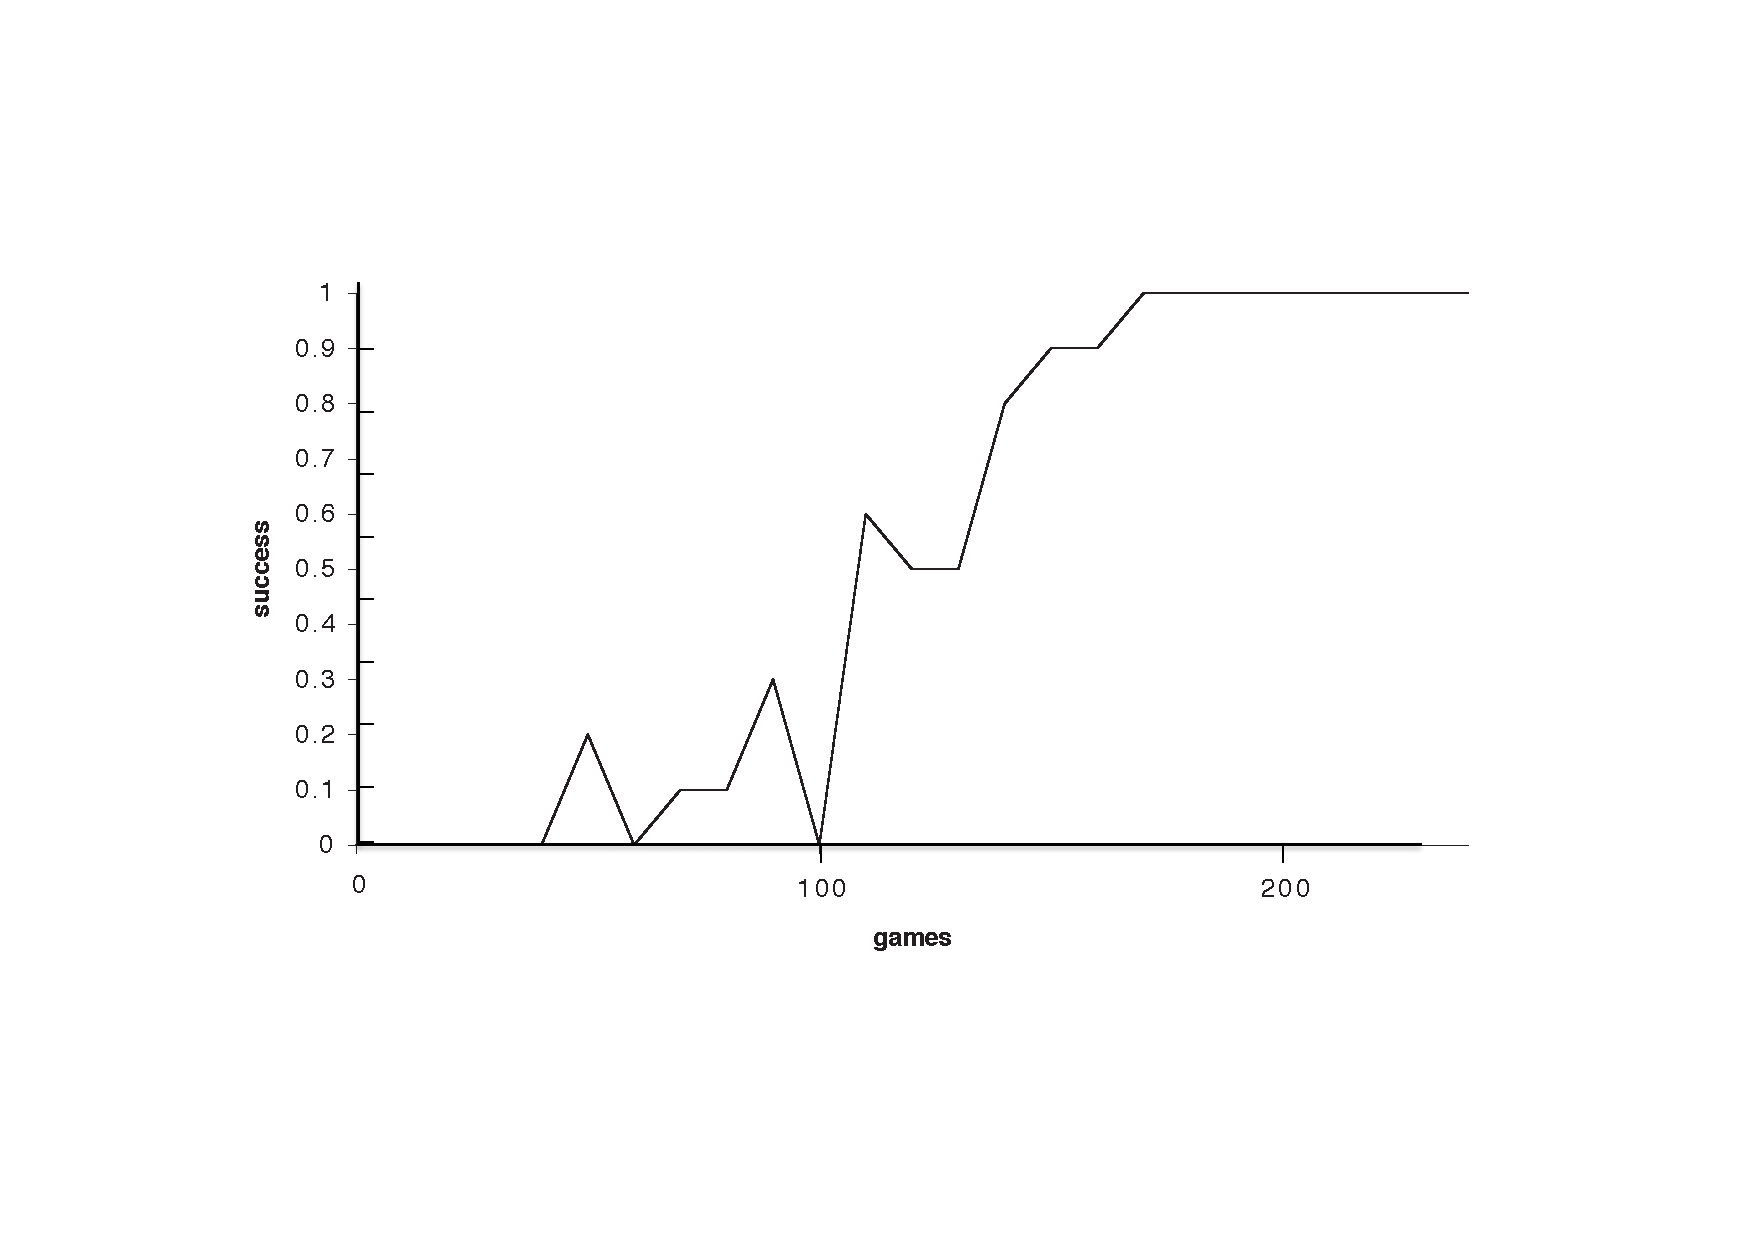
\includegraphics[width=.70\textwidth]{chap5/figs/success}}
\caption{ \label{success} 
The graph displays on the y-axis the average success every 10 games
in a population of five agents lexicalising five
different meanings. The x-axis 
shows the number of games. Average success
rapidly climbs until it reaches total success after 
about 180 games.}
\end{figure}

When the population (both of meanings and agents) is larger, 
one would expect that it takes longer to reach total average
success. This is indeed the case (\figref{larger}). 

\begin{figure}[htbp]
  \centerline{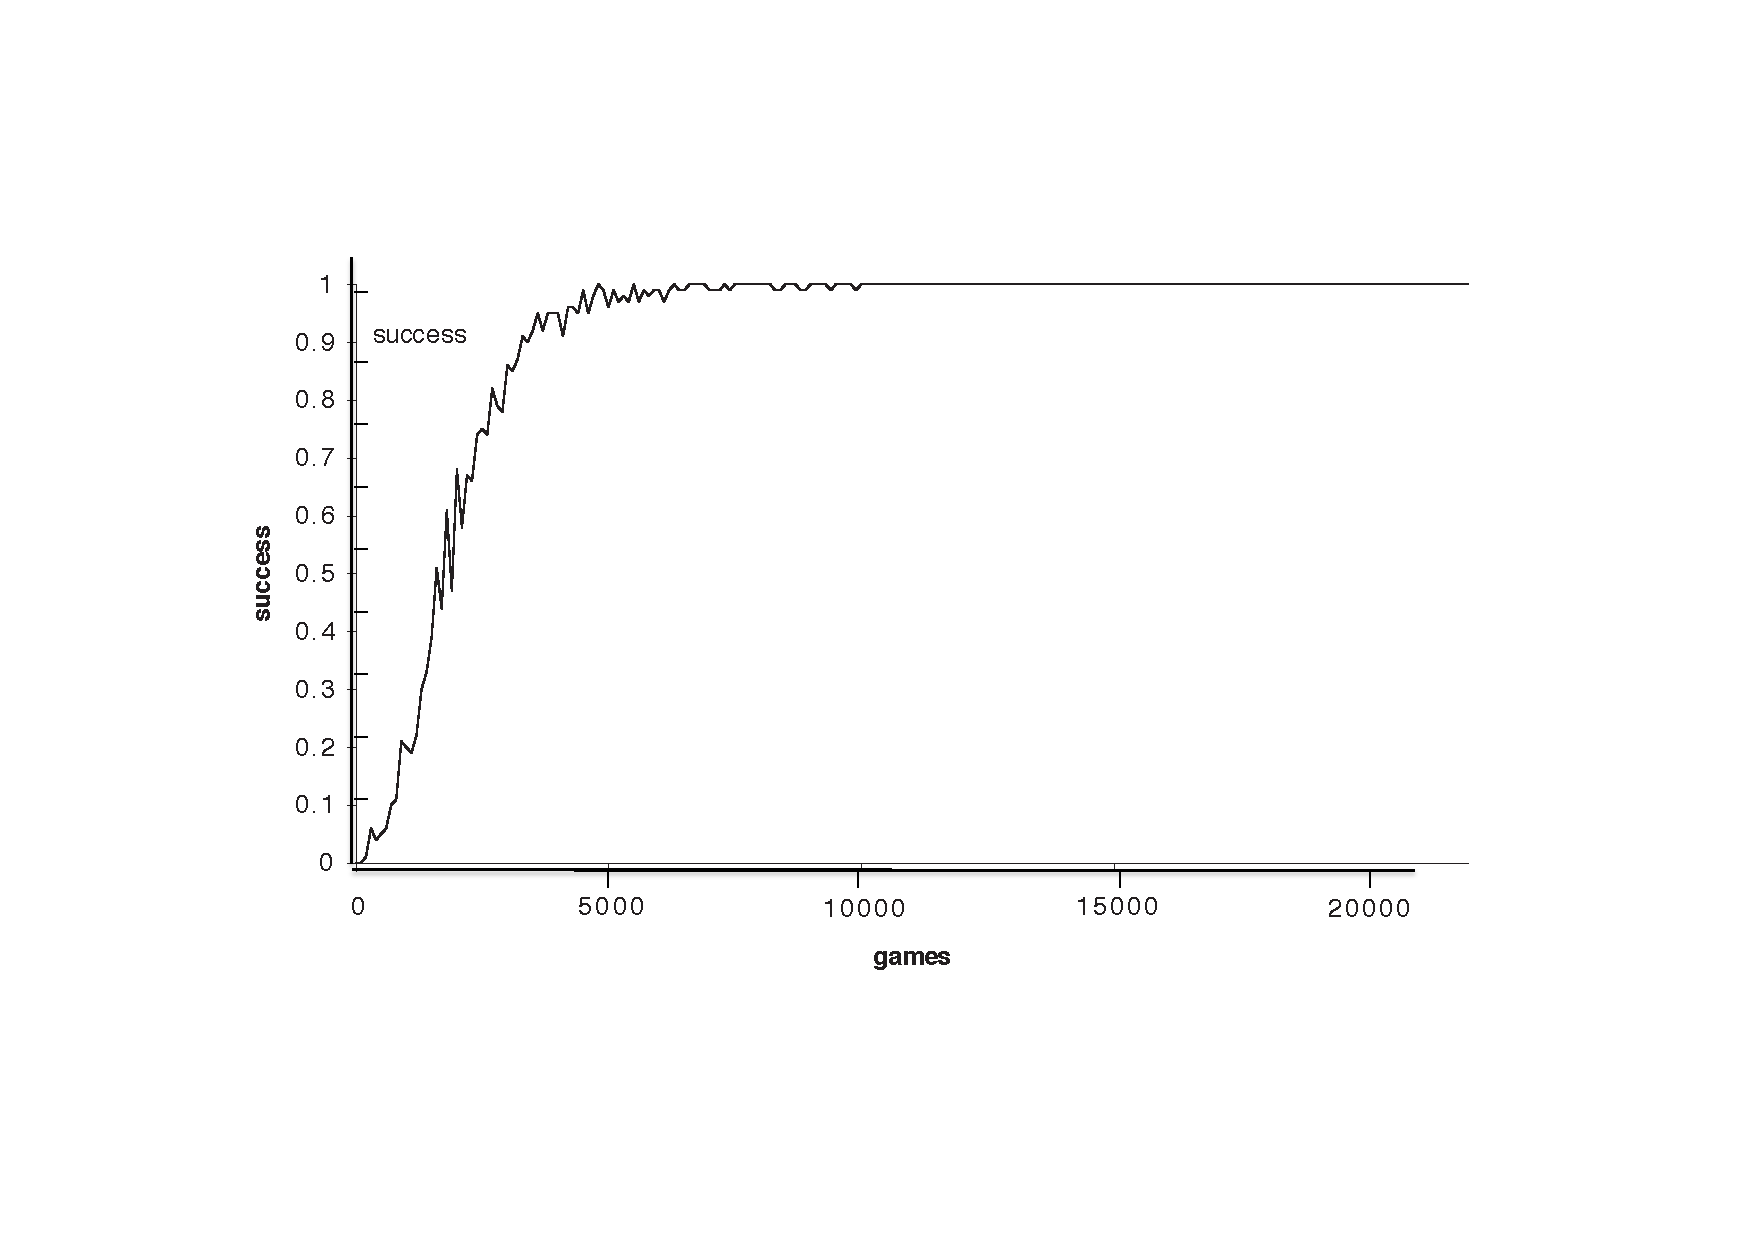
\includegraphics[width=.70\textwidth]{chap5/figs/larger}}
\caption{\footnotesize \label{larger} 
The graph displays the evolution of communicative success
for larger and larger populations. The
number of games on the x-axis
is divided by the number of agents. }
\end{figure}
We see for example that for 20 agents and 20 meanings 
success climbs to total success after about 10,000 games.
This is still surprisingly low particularly as
success is
are already above 95 \% after about 5000 games. Games can be played
in parallel by different agents because the system 
is entirely distributed. If we divide
the number of agents by the number of games, we see that about 250
games are needed by the agents to get 95 \% success, which means
that every meaning needs to appear about 10 times for each agent. 
Interestingly enough, the larger the population of agents, 
the more the success curve approximates an 
S-shape, which has 
been observed empirically in the spreading of new
linguistic conventions. The same curve shape is familiar to
biologists studying models of competitive growth, suggesting 
a strong relationships between ecological dynamics and language\is{S-shape curve}
spreading.\footnote{The S-shaped curve is discussed in \cite{McMahon:1994} p. 52. For examples
of biological models with similar properties, see \cite{May:1976}.}

\subsection{Measuring lexical coherence} 

To monitor to what extent the agents share the same
lexicon, I propose a second measure, the {\itshape lexical
coherence}. The lexical coherence is 
defined as the average of the frequencies of
all the form-meaning pairs in the group lexicon.
If all agents prefer the same form-meaning 
pair for all meanings, lexical coherence is 1.0. If they agree
on none, it is 0.0.\is{lexical coherence}

Consider the following group lexicon after 3000 games for the
previous simulation (with 20 agents), shown in \tabref{tab:t-mem3000}. 

\begin{table}
\begin{center}
\begin{tabular}{l  l  l  l  l  l }
\lsptoprule 
{\itshape meaning} & {\itshape form} & {\itshape frequency} & {\itshape meaning} & {\itshape form} & {\itshape frequency} \\ \midrule
{}[DARK]& dato & 1.00 & [LARGE]& biti & 0.80 \\  
{}[LIGHT]& pitu & 0.60 & [SMALL]& dopu & 1.00 \\  
{}[RED]& gabi & 1.00 & [GREEN]& gu & 0.85 \\  
{}[SQUARE]& koti & 0.50 & [RECTANGLE]& totu & 0.65 \\  
{}[LEFT]& toga & 0.90 & [BLUE]& ku & 0.80 \\  
{}[YELLOW]& gubo & 0.55 & [CHARMING]& ge & 1.00 \\  
{}[TRIANGLE]& bu & 0.85 & [SQUARE]& ba & 0.60 \\  
{}[FAST]& beke & 1.00 & [SLOW]& tu & 0.95 \\  
{}[CIRCLE]& ke & 0.75 & [RIGHT]& gaba & 0.95 \\  
{}[UP]& butu & 1.00 & [DOWN]& ki & 0.95 \\  
\lspbottomrule
\end{tabular}
\caption{\label{tab:t-mem3000} Group lexicon after 3000 games.}
\end{center}
\end{table}
The lexical coherence is at this point equal to 0.835. 

Lexical coherence can be graphed alongside
average success (see \figref{suc-coh}). As expected, 
lexical coherence increases 
and we can see that as coherence increases the success
rate increases.

\begin{figure}[htbp]
  \centerline{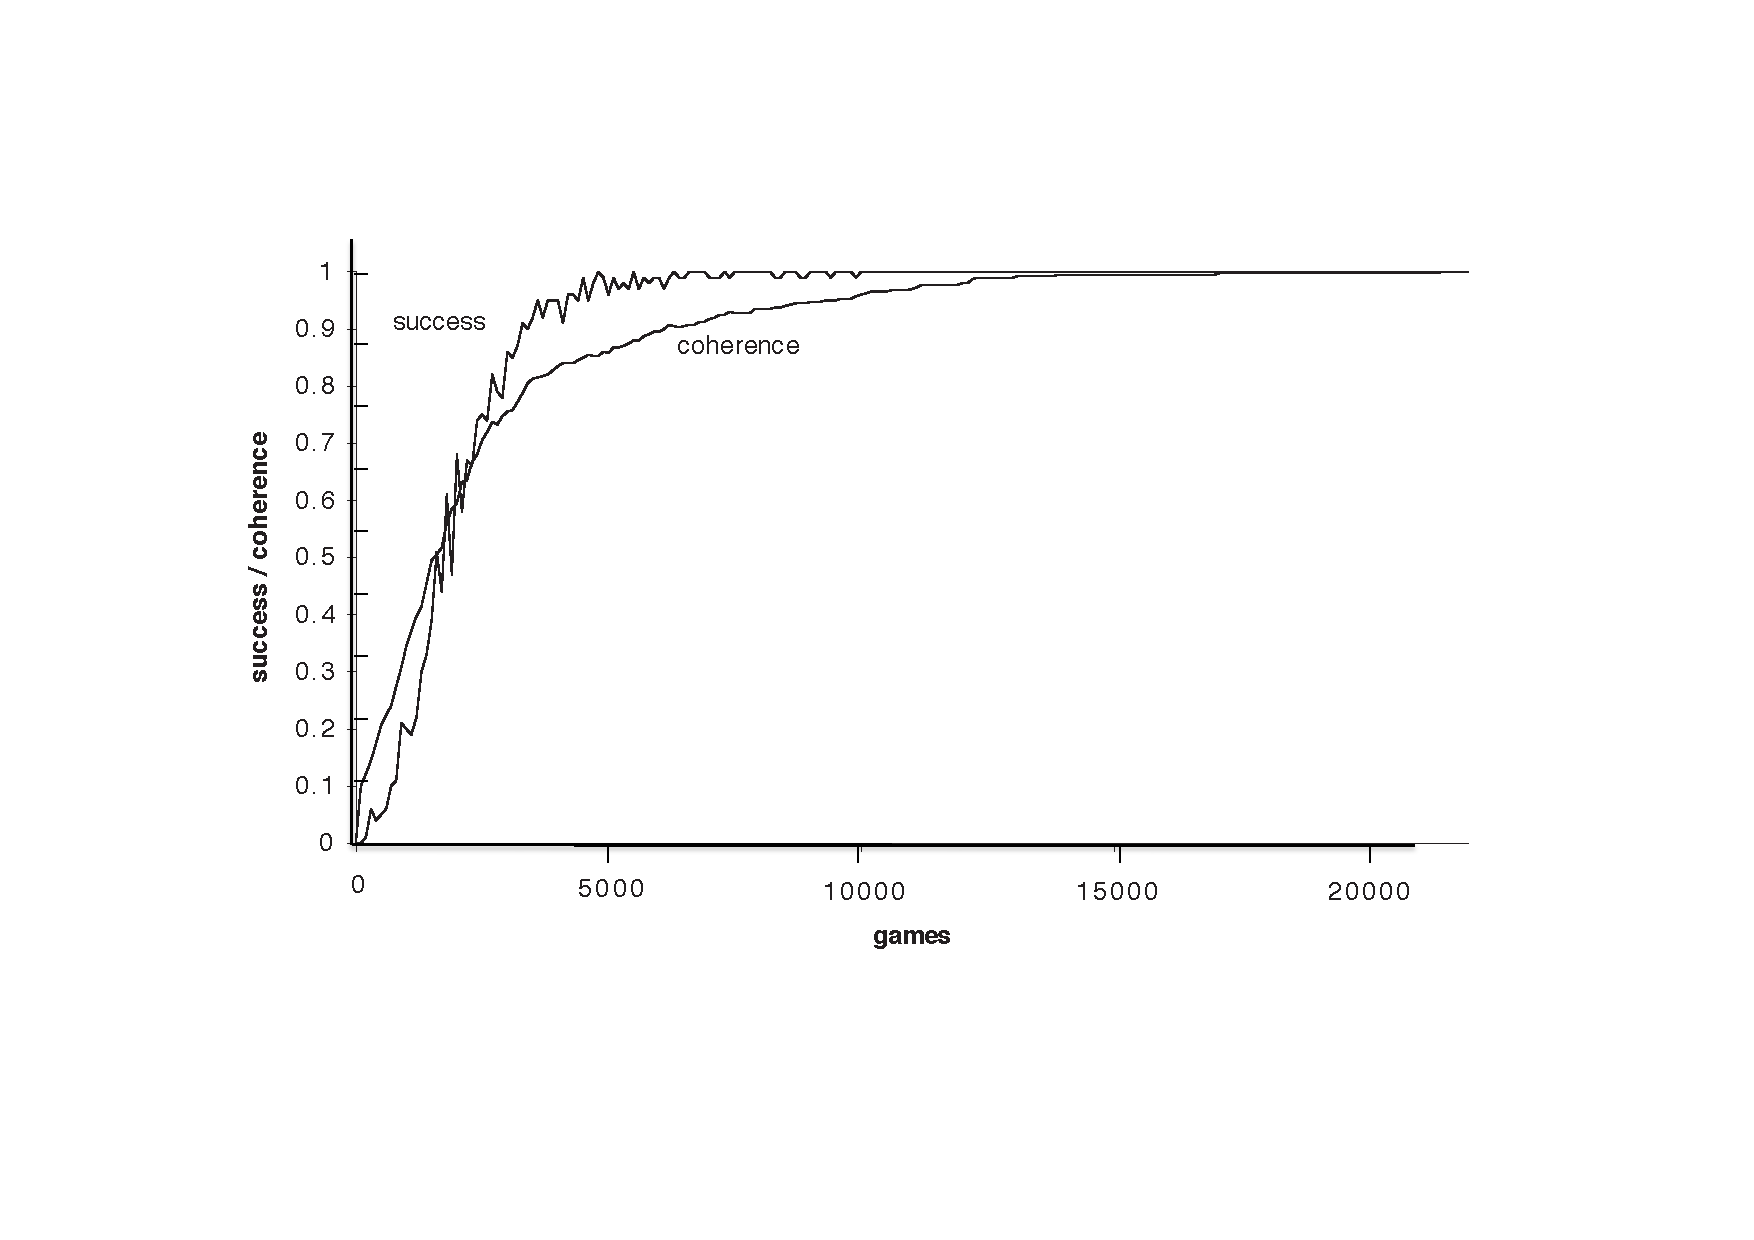
\includegraphics[width=.70\textwidth]{chap5/figs/suc-coh}}
\caption{\label{suc-coh}This figure shows the evolution of both average
success and lexical coherence for a group of 20 agents and 20 
meanings. Total lexical coherence climbs more slowly
once the 
population has reached a high average success.}
\end{figure}
Does total success imply that all agents use the 
same lexicon? Not really. To have success, the hearer
must associate the form used by the speaker
with the same meaning. But it is not required that the
hearer himself prefers to use the same form for the same meaning, 
synonyms may occur.  
A speaker of British English typically uses the word ``pavement'', 
whereas an American prefers ``sidewalk'', even though he
understands ``pavement''. Thus there can 
be several forms active in the same population, even though 
the outcome of a game is always successful. We will see 
later that synonyms do get damped, as is the case in 
human natural lexicons. 

Initially lexical coherence is higher than success, because a game 
fails if the hearer is acquiring the form-meaning association
used by the speaker. So two agents could have stored the same association, 
and thus coherence would have increased, without already having enjoyed the benefit
in a successful communication. However, once success
is total, agents no longer make changes based on negative feedback
from failure, simply because there is no failure,  
even the less common forms are understood correctly 
by everybody. Further progress towards more coherence
is therefore only due to the 
fact that the more common forms occur more often so that
their scores keep going up as they are used more. 

\section{Scaling up} 

The associative memory and the score updating introduced
in the previous section appears to allow a group of 
distributed agents to establish a shared repertoire of
form-meaning pairs. Of course, I still need to show that 
this mechanism remains adequate when it is incorporated
in a complete game, in which case there is no direct feedback 
about meaning. But before doing so, let us see whether 
the mechanisms are adequate from the viewpoint of scaling: 
Can they handle variation in the set of meanings to 
be expressed? Do they cope with a changing population? 

\subsection{Coping with new meanings}

In natural languages, new meanings arise every day 
while other meanings become irrelevant. 
For example, none of the terms used for talking about
the Internet (e-mail,
surfing, home page, etc.) would have made sense to anyone
a few decades ago. On the other hand, most of us now have lost 
many categories and concepts for classifying plants, 
simply because they are no longer such a prominent part of our 
urbanised environments. It follows that a mechanism 
claiming to explain the origins and acquisition 
of a lexicon in a population
of agents should cope with a fluctuating set of meanings
as well. This property is moreover crucial in the Talking 
Heads experiment because new meanings will continuously 
arise as the agents encounter new situations in 
the environment. 

Because the Naming Game included ways to 
handle new meanings from the start, nothing should 
have to be changed to handle an increased set of meanings. 
Let us see whether the Naming Game indeed copes
through the next simulation (see \figref{inoutmean}), using 
arbitrary labeled meanings ([M1], [M2], etc.). 
In a first phase, the system is closed 
and a shared lexicon emerges for the initial set 
of 20 meanings, as expected. The group's lexicon
is now as in \tabref{tab:gphase1}. 

\begin{table}
\begin{center}
\begin{tabular}{l  l  c  l  l  c } \lsptoprule 
{\itshape meaning} & {\itshape form} & {\itshape frequency} & {\itshape meaning} & {\itshape form} & {\itshape frequency}\\ \midrule 
{}[M1]& gebo & 1.00 & [M2]& goge & 1.00 \\  
{}[M3]& koto & 0.70 & [M4]& da & 1.00 \\  
{}[M5]& peko & 1.00 & [M6]& ki & 1.00 \\  
{}[M7]& gipe & 1.00 & [M8]& kedo & 1.00 \\  
{}[M9]& do & 1.00 & [M10]& gige & 1.00 \\  
{}[M11]& pi & 1.00 & [M12]& bu & 1.00 \\  
{}[M13]& pa & 1.00 & [M14]& kipa & 1.00 \\  
{}[M15]& depi & 0.95 & [M16]& pudi & 1.00 \\  
{}[M17]& tegi & 1.00 & [M18]& ba & 0.90 \\  
{}[M19]& ko & 1.00 & [M20]& guda & 1.00 \\  
 \lspbottomrule
\end{tabular}
\caption{\label{tab:gphase1} Group lexicon after first phase.}
\end{center}
\end{table}
In phase 2, a relatively small meaning flux is introduced (one
new meaning every 1000 games). As can 
be seen from \figref{inoutmean}, 
the population copes with the change. New words are created and 
propagate in the population. The following group lexicon
shows that for newcomers like [M22] or [M25] a total 
consensus has emerged. Words for the latest
new meanings, [M28] and [M29], still have low frequencies. 

\begin{table}
\begin{center}
\begin{tabular}{ l  l  c  l  l  c } \lsptoprule 
{\itshape meaning} & {\itshape form} & {\itshape frequency} & {\itshape meaning} & {\itshape form} & {\itshape frequency}\\ \midrule 
{}[M1]& gebo & 1.00 & [M2]& goge & 1.00 \\  
{}[M3]& koto & 1.00 & [M4]& da & 1.00 \\  
{}[M5]& peko & 1.00 & [M6]& ki & 1.00 \\  
{}[M7]& gipe & 1.00 & [M8]& kedo & 1.00 \\  
{}[M9]& do & 1.00 & [M10]& gige & 1.00 \\  
{}[M11]& pi & 1.00 & [M12]& bu & 1.00 \\  
{}[M13]& pa & 1.00 & [M14]& kipa & 1.00 \\  
{}[M15]& depi & 1.00 & [M16]& pudi & 1.00 \\  
{}[M17]& tegi & 1.00 & [M18]& ba & 1.00 \\  
{}[M19]& ko & 1.00 & [M20]& guda & 1.00 \\  
{}[M22]& to & 1.00 & [M23]& de & 0.85 \\  
{}[M24]& tabo & 0.95 & [M25]& piku & 1.00 \\  
{}[M26]& ku & 1.00 & [M27]& pugu & 1.00 \\  
{}[M28]& tete & 0.35 & [M29]& todu & 0.35 \\  
\lspbottomrule
\end{tabular}
\caption{\label{tab:phase1} Group lexicon after second phase.}
\end{center}
\end{table}
Next (phase 3 in \figref{inoutmean}) a much higher 
meaning flux is imposed (one new meaning every 100 games). 
Lexical coherence decreases and
average success plummets. There is not enough time to propagate
the new conventions in the group. 
Note that lexical coherence drops slower than 
success when the lexicon disintegrates. 
Coherence is based on the average for all 
meanings, thus only the new ones are therefore affecting overall coherence. 
Success drops more rapidly 
because of the high rate of failure of new meanings. 


\begin{figure}[htbp]
  \centerline{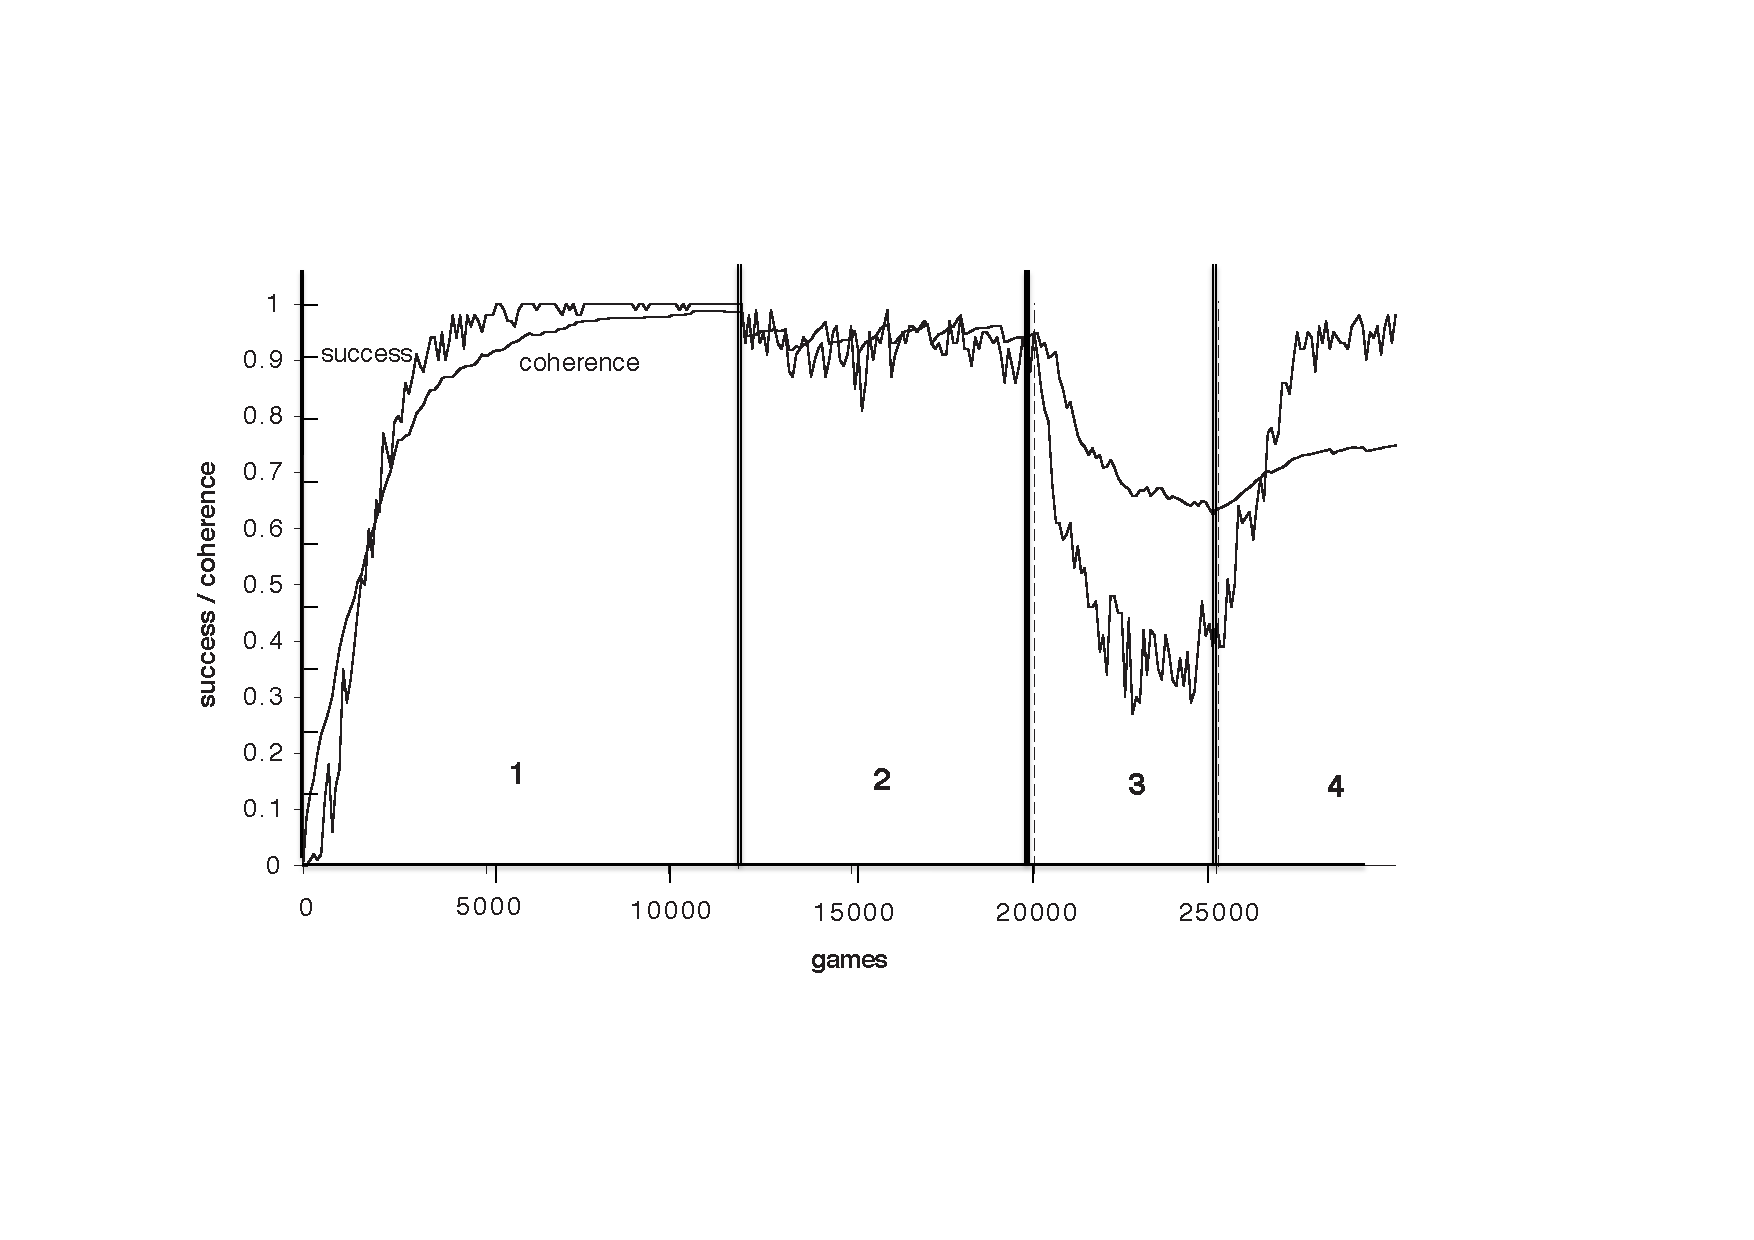
\includegraphics[width=.70\textwidth]{chap5/figs/in+out}}
\caption{ \label{inoutmean}  Both average success (every 100 games) and lexical coherence 
is shown in cases of an inflow of meanings for a population 
of 20 agents starting with 20 meanings (phase 1). The inflow 
is 1/1000 in phase 2, 1/100 in phase 3 and 1/1000 in phase 4.}
\end{figure}

The system restores itself
when the flux of meaning is brought back to 1/1000 games
(phase 4). Interestingly enough, coherence now increases slower
than success. 
The instability caused by a rapid influx of new meanings has lead 
to many new forms for the same meanings. These synonyms
now spread in the population and lead to a rapid
increase in communicative success. Coherence
climbs up more slowly because competing synonyms 
are only gradually weeded out, based on their frequency of use. 

We can conclude that the agent architecture
manages to handle an influx of meaning, as long as the flux 
stays within certain bounds. 

\subsection{Lexicon acquisition by virgin agents}

The next question we need to investigate
is whether the mechanisms 
explain how a lexicon, once it has formed, can 
be preserved from one generation to the next. This clearly 
happens in human populations. Although lexicons show
profound change, large parts get preserved even over 
very large periods of time. 
Some linguists even claim that the roots of certain 
words still in use today go back to the very beginnings
of language which is hypothesised to 
have been around 50,000 
years ago.\cite{Ruhlen:1994}
A genetic solution, where the lexicon is stored in the genetic 
code and thus transmitted from parent to child, seems clearly 
out of the question. Nevertheless, a lot of the 
early work on computational modeling
of language origins relied on a genetic approach 
for transmitting the lexicon, possibly with some
additional adaptation. See for example: \cite[603--631]{MacLennan:1991}.
This approach sheds light on the issue how signaling
systems may evolve in animals but is not applicable
to the transmission of human lexicons. The lexicon of human languages 
is too diverse and changes too quickly to allow genetic
transmission. So lexicons must somehow be transmitted 
in a cultural process.

It turns out that the agent architecture I introduced
in the previous sections does not 
need to be changed at all to obtain a cultural 
transmission of a lexicon, illustrating the explanatory 
power of the model despite its simplicity. New virgin agents
entering the group may occasionally create a new word, 
if they do not have one themselves, but if a 
particular set of words with particular meanings
is already strongly entrenched in the population, these
new words have a very low probability to survive.
Instead, the virgin agents will adopt the words
that they abundantly hear in their environment, and the
score of these words goes up quickly. 

Here is a computer simulation testing whether this 
is indeed the case (see \figref{birth}). 
We begin with a population of 20 agents and let them develop a 
shared lexicon for 20 meanings (phase 1). Then I {\itshape add}
new virgin agents at regular time intervals, at a rate 
of 1 every 1000 games (phase 2). A new 
agent has no knowledge of the existing lexicon and
therefore must acquire the lexicon present in the rest
of the group. \figref{birth} (phase 2) shows that the 
population indeed copes. A new member initially causes 
some failures in communication, but he quickly
picks up the lexicon of the community and success
moves back up. The lexicon does not change, it is 
stable against minor perturbations. 


\begin{figure}[htbp]
  \centerline{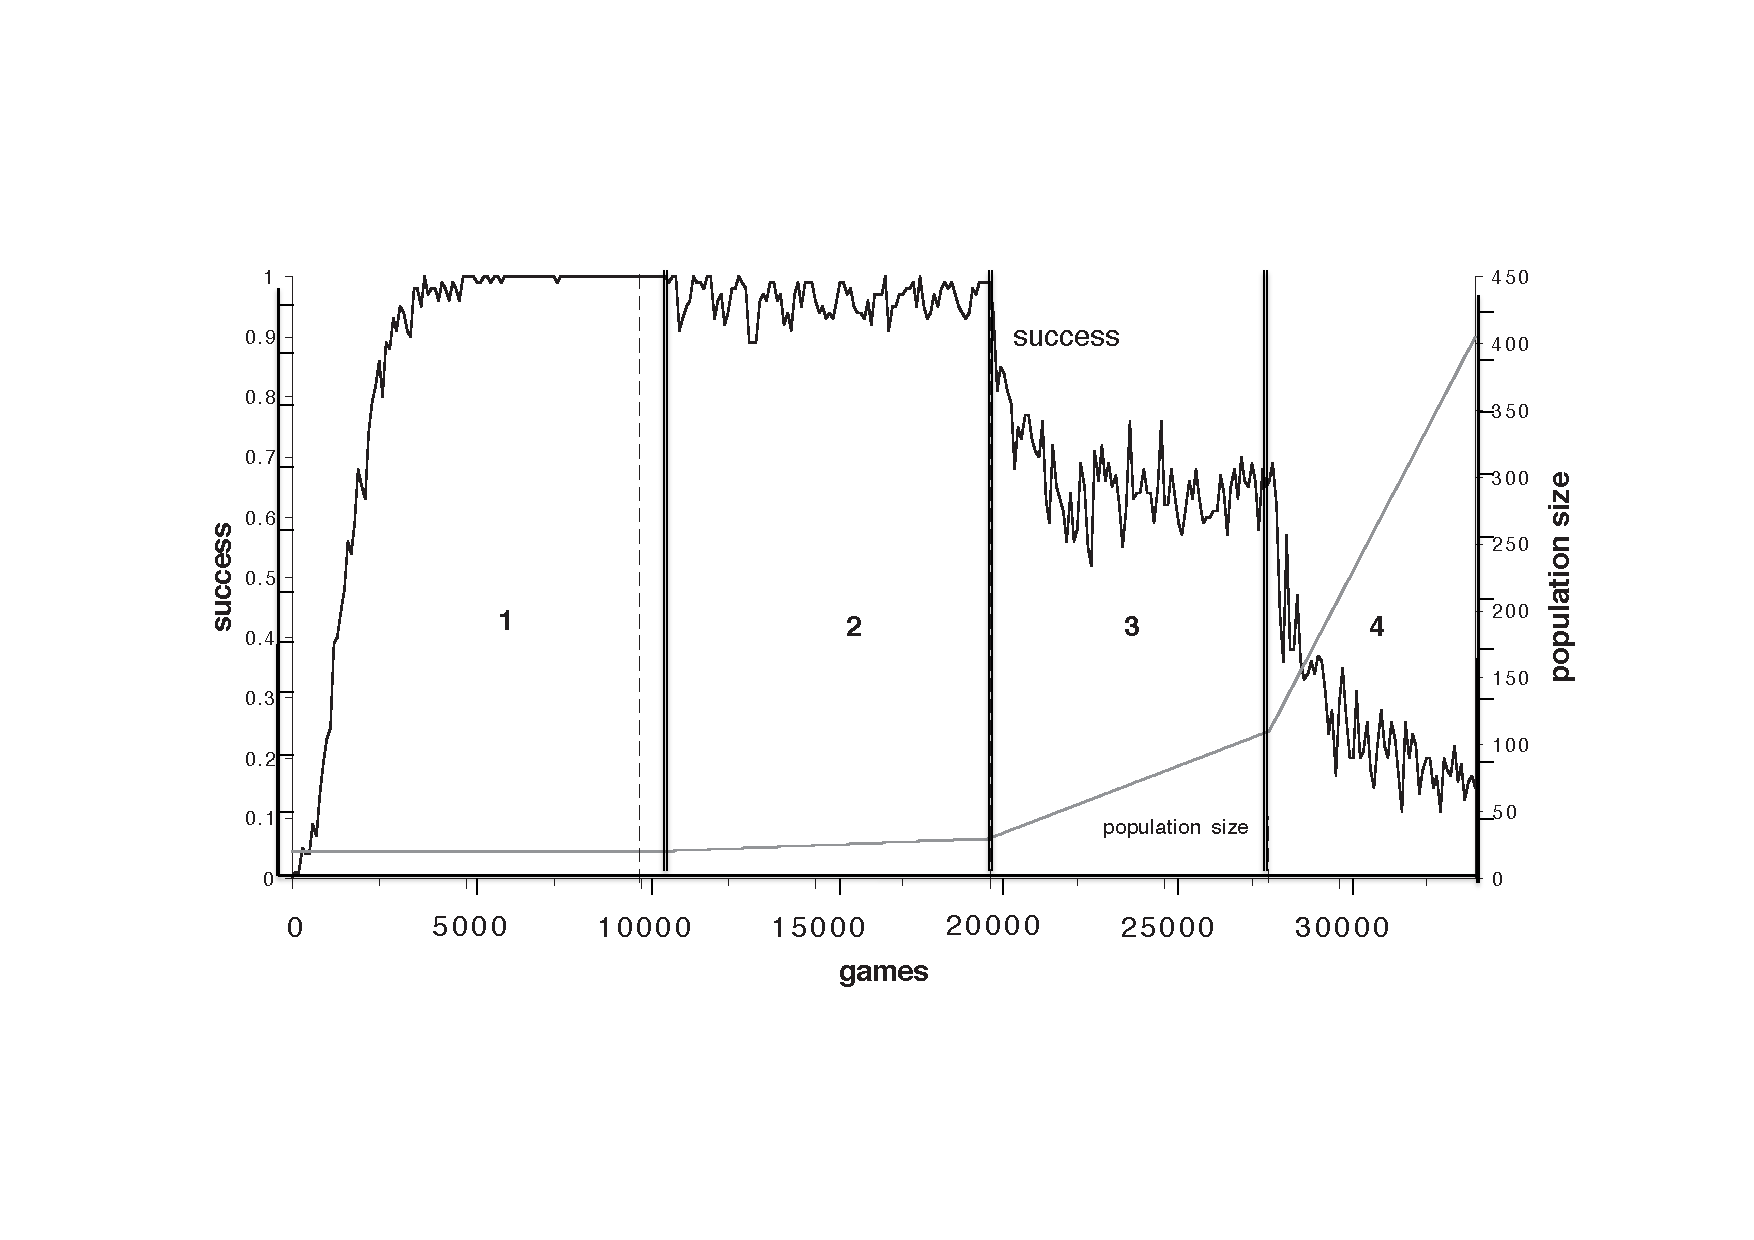
\includegraphics[width=.70\textwidth]{chap5/figs/birth}}
\caption{\label{birth} Evolution of communicative 
success with different birth-rates, starting from a
population of 20 agents (phase 1). 
Next the birth rate is increased from 1 new agent 
every 1000 games (phase 2) to 
1 new agent every 100 games (phase 3), 
and then to 1 every 50 games (phase 4).}
\end{figure}

However, when the birth rate is increased
to 1/100 games (phase 3) the population is less able to cope. 
Success stays relatively high (70 \%), but there are too many 
new agents coming in too fast. The lexicon cannot spread 
sufficiently quickly to the new agents and therefore starts 
to disintegrate. In a final stage (phase 4), the birth rate 
is set again to 1 new agent every 50 games. The population is no longer  
able to cope with the influx of new members and disintegrates. 
If inflow is brought back to a lower rate, the population would 
again establish a shared lexicon. However, 
the lexicon is now a different one
from the one that was established before. 
The dynamical process
has moved from one stable lexical state to another one.  

We have seen earlier that the Naming Game scales
up with respect to the size of possible meanings. Now 
we see that it scales up with respect to the size of 
the population. As long as the rate of influx is not too
high, the population can keep expanding. 
The only constraining factor is that new agents
must have sufficient opportunities to acquire the lexicon
present in the group. 

\subsection{Preservation in changing populations}

In human populations, there is not only an influx of 
new members but also an outflux. When somebody leaves
the community knowledge about the lexicon should
disappear as well. Nevertheless, a lexicon clearly 
gets preserved from one generation to the next, which 
implies that the know-how is distributed robustly over
the agents.\is{population change}

The next computer simulation tests whether this is also true
in the Naming Game model. 
The simulation starts with a population of 20 agents who 
are left to develop a shared lexicon for 
20 meanings (phase 1). 
Then an in- {\itshape and} out-flux is introduced (phase 2 in 
\figref{birth+death}) with one
new virgin agent coming in 
and another agent leaving the population every 1000 games. 
The new agent has to acquire the lexicon present in the group. 
Average success therefore dips but is quickly regained.
In fact, the population can be completely renewed without affecting the
lexicon at all. 
After 16000 games nine agents (50 \%) have been
replaced, but the lexicon has not changed. So, the Naming Game model
not only explains the formation of 
a lexicon but also its transmission: This transmission is 
entirely cultural. New agents enter the population with no 
prior knowledge. 


\begin{figure}[htbp]
  \centerline{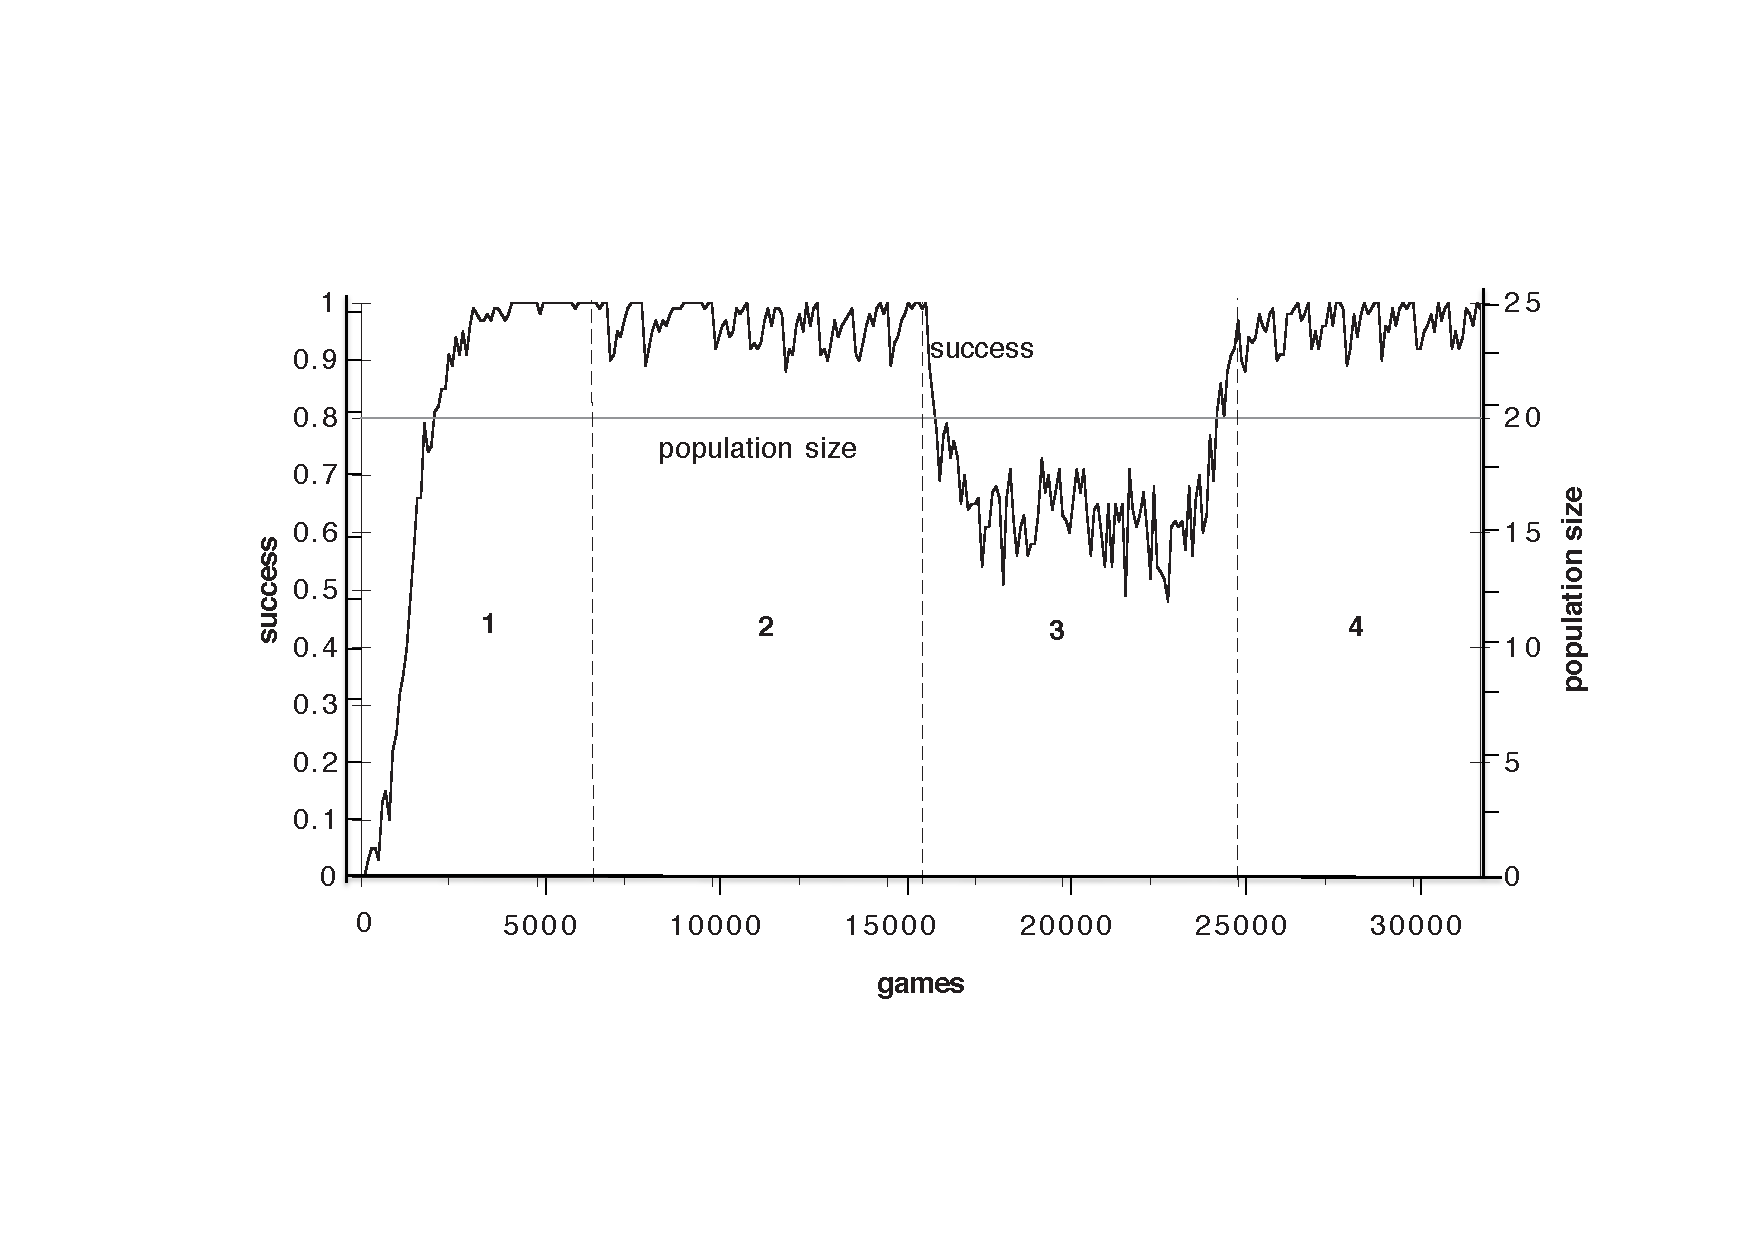
\includegraphics[width=.70\textwidth]{chap5/figs/birth+death}}
\caption{\footnotesize \label{birth+death} Success and population size 
is shown for a series of 35,000 language games. 
The population starts with 20 agents and 20 
meanings (phase 1). Then an influx and outflux is introduced 
at the rate of 1/1000 games (phase 2). The lexicon
maintains itself. In phase 3 agents enter and leave at
the rate of 1/100 games. Success lowers. In phase 
4 the rate of change is brought back to 1/1000 games
and success is regained.}
\end{figure}

Can we increase the flux in the population indefinitely? 
This is examined in phase 3 of \figref{birth+death}. 
In this phase a higher flux has been introduced. One agent is added
and removed every 100 games. Success goes down, although it is still maintained at a high 
level. The lexicon is still not changing. 
However, previous examples have already shown us 
that if we continue to increase the rate, the
lexicon would disintegrate. 
Too many new agents would be flowing in, who do not have
a lexicon yet. On the other hand, if we bring the rate of change 
back down to 1/1000 games (phase 4 in figure 
\ref{birth+death}), success regenerates. 

These simulation illustrates how we can study lexicon
transmission using a language game approach. We have
to set up an in- and outflow of the agents and 
study the impact on their communicative success
and their lexicon. In principle, we should 
not have to change the architecture of the individual 
agents, and indeed I have not done so. Language acquisition 
is such an integral part of language use that a realistic 
agent architecture must intimately integrate both capacities
from the start. Of course, at this stage 
we have only tested this
with the agents getting direct feedback about meaning, 
we still must that whether it will continue to work
with the physically instantiated Talking Heads. 

\section{Self-organisation}

These various simulations show that the Naming Game embodies robust
mechanisms for the emergence of a lexicon and we will use it 
as a core component for the Talking Heads experiment. 
In retrospect, the following mechanisms 
are crucial for the success of the model:\is{lexical self-organisation}
\begin{enumerate}
\item Agents must be able to represent multiple associations
(one form can be associated with many meanings and one
meaning with many forms). Multiple associations 
naturally arise in a population of distributed 
agents because an agent may create a new form not 
knowing that one already exists in the population, or
guess a different meaning for a form than the one
intended by the speaker. I will discuss such examples in
more detail later. 
\item An agent must be able 
to record a score for each association. The score is necessary
for the agent to decide which meaning or which form should 
be preferred in a particular interaction. When random 
choices are made lexicons do not converge. 
\item Agents must be able to create new words when no words are 
available yet. When there is a fixed set of words, the problem 
is much harder and the distributed search 
process may get stuck into local minima. 
Lexical systems must be able to cope with 
a steady influx of new meanings so restricting the set 
of words from the beginning would be odd. 
\item Agents must perform lateral inhibition, which means that 
they must decrement the score of competitors to the
form-meaning pair which won a competition. 
This is necessary to achieve convergence. 
\item Agents must get feedback in the case of failure. At the moment
the feedback is direct, but I will soon embed the naming game
into a more complex guessing game in which feedback comes
from the externally observed outcome of the language 
game as opposed to the direct transmission of the intended meaning. 
\end{enumerate}
When any of these characteristics of the agent
architecture or the game
are eliminated, the system does not work. Communicative success
does not climb, convergence will not go beyond a small percentage, 
the size of the lexicon explodes, and so on. The fact that 
these architectural properties are crucial and non-trivial to 
discover strongly suggests that similar mechanisms must be in 
place in the emergence of human lexicons. 

It is also important to stress what is not in the model. 
The mechanisms used by the agents are deliberately kept as 
simple as possible. Complexity should arise only from the 
enactment of simple construction rules. Agents do not 
go through complex reasoning about words, they simply 
store the new associations they encounter and rely on 
the updating processes to weed out wrong hypotheses. 

\subsection{Winner-take-all processes}

The most remarkable and at first mysterious property of the 
Naming Game model is that the agents somehow reach a consensus
without any central supervisor. They do {\itshape not} do this by 
having a general overview or by changing their internal 
parameters so as to become more conservative as the lexicon
solidifies. It is solely due to the subtle interaction between
language use, which gradually becomes uniform, and each agent's
adaptation to the language heard in the environment. 
If a certain word comes to be preferred by a group of agents
for a certain meaning, its frequency of use goes up so that
others encounter this 
word more often and hence their scores for that word
continue to increase as well.
The more agents use a word, the higher its chance of success
and the more it will be used. This effect is still enforced 
by lateral inhibition. The scores of competing associations 
decrease, making it less likely that they will win in the future. 
This positive feedback therefore introduces an\is{autocatalysis} 
{\itshape autocatalytic} (self-enforcing) effect until the population
locks into an equilibrium state.\footnote{
Such positive feedback loops and the stability criteria
associated with them have been widely studied in non-linear
dynamical systems and applied to chemical and biological 
processes. See \cite{Babloyantz:1986}.}

To follow better how a consensus gradually emerges, I will visualise
the competition between different words for the same meaning
in a {\itshape meaning-form (MF) competition diagram}, 
such as the one in \figref{competition}, which monitors 
the frequencies of the different forms in use for one meaning.
The diagram shows clearly the struggle between different forms until
one form (``pe'') emerges as the winner. When we later study 
grounded lexicon formation processes, we will see that the 
competition becomes much more complex and the whole system 
is in constant evolution. A form-meaning pair which is 
dominating may become weaker because its meaning
fails to pick up the right
referent in a new context. 
This in turn may trigger the creation of new words or the 
resurgence of existing words. 

\begin{figure}[htbp]
  \centerline{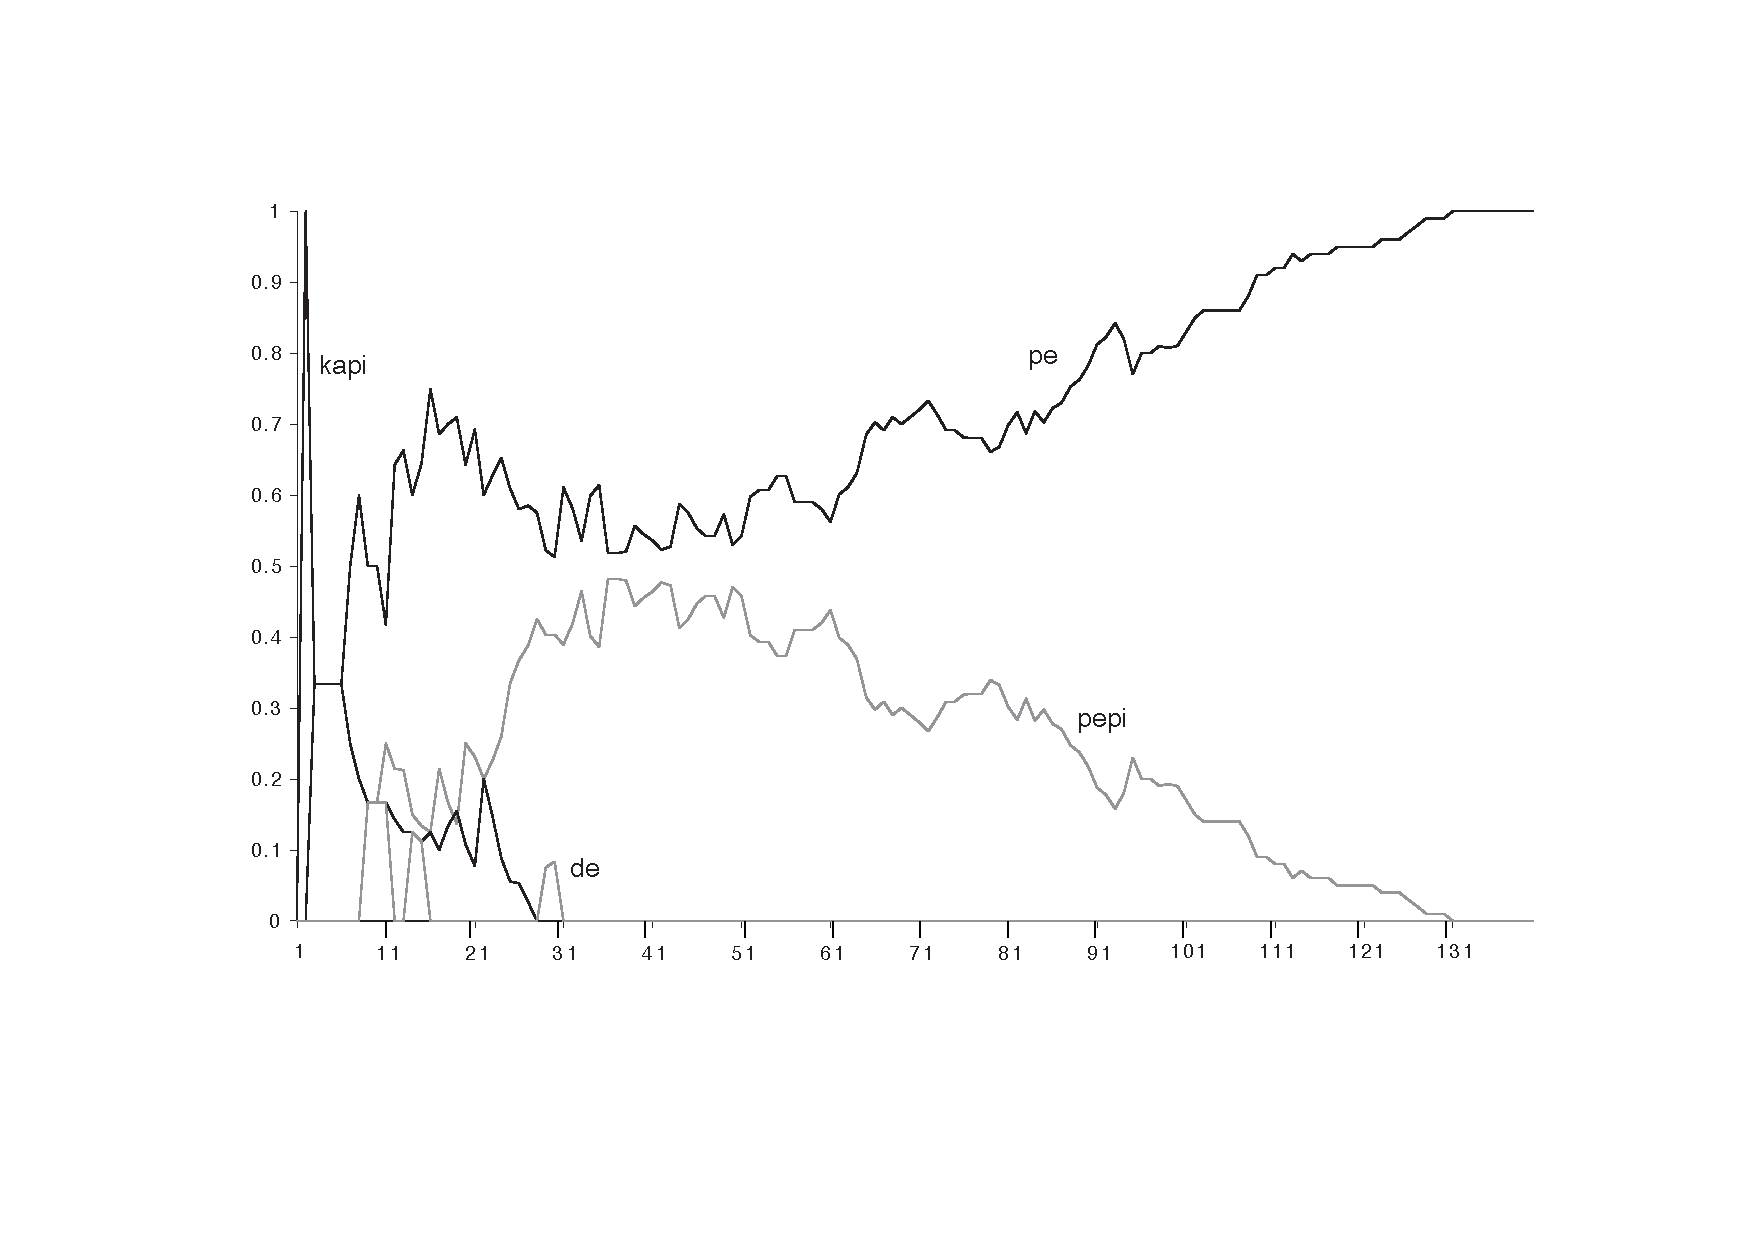
\includegraphics[width=.70\textwidth]{chap5/figs/comp1}}
\caption{\label{competition} Simulation with 
a population of 20 agents. The meaning-form competition 
diagram shows the frequency of all competing forms for a 
single meaning. We see a winner-take-all situation
with one word (``pe'') dominating.}
\end{figure}

\subsection{Collective Behavior and Self-organisation}

Biology is full of examples where structures spontaneously 
self-organise from the unco-ordinated activity 
of distributed elements through a winner-take-all process.
Each time the same basic components as in the Naming Game model
are seen: Random behavior creates various possibilities and the 
reinforcement of some of these variations through positive
feedback creates an autocatalytic effect. 
Perhaps the clearest examples can be found 
in the collective behavior of 
social insects, such as the formation of nests by termites, 
although beautiful explanations have also been reported
for the formation of patterns on sea shells, the growth of
cell tissue, the aggregation
of individual cellular slime mold amoebae into a slug, 
the flocking and collective movement of birds or mammals, 
etc. (\cite{Meinhardt:1982}). A classical 
example for collective behavior, first developed by Jean-Louis 
Deneubourg, is the formation of paths in an ant society through 
mass recruitment, \cite{Pasteels:1987}. 

When ants carry food or other materials, they organise themselves in a
chain which is typically the shortest path between the source and the nest. 
These chains can sometimes be surprisingly long (20 meters is 
quite common for European ants) and are 
maintained as long as the food supply lasts. The whole process has many
intriguing properties. First of all, there is
no central planning agency that regulates which food sources 
are to be explored. The coherence and co-ordination between hundreds
or sometimes thousands of ants is established in a 
completely distributed fashion. There is no dependence 
on individual ants. Ants can 
be removed from a path or new ones can be introduced randomly without too 
much interference for the stability of the path as a whole. The paths are
robust. If objects are put in the way or if the path is destroyed, 
the ants manage to reestablish it in a relatively short time span. 
The paths are adaptive. If the food supply terminates, the path 
disintegrates and a new path will appear linking the ants to an alternative 
food source. 

We see here many of the properties found in natural languages
and integrated in the Naming Game model: 
absence of central planning, no critical dependence on a 
single element, resilience to influx or outflux of elements, and
adaptation to changing circumstances. Even more interestingly, 
the ants manage to establish these dynamic paths by a process 
which is similar to the language formation process used in the 
Naming Game, namely a positive feedback loop having an autocatalytic
effect. An individual ant appears to move around in a random fashion 
while searching for a source of 
food. When a food source is discovered, the ant returns to the nest 
using a global landmark like the sun. 
The food-carrying ant also deposits a chemical substance 
known as a pheromone as he travels back to 
the nest. This pheromone influences the 
otherwise random movement of the other ants, in that ants are 
attracted by the pheromone. Thus more ants are drawn to the path and hence
led to the food source. As these ants in turn go back
to the nest they also deposit 
pheromone. This gives the self-enforcing, autocatalytic
effect: The more ants are on the path, 
the more pheromone is deposited, and therefore the stronger 
the attraction to the other ants.
Very soon all the ants which were sufficiently close 
to the path form a chain. There is no central planning agency 
needed and the whole system does not depend on an individual ant. The 
order is emergent. 

These simple mechanisms also explain other features of the process. 
When the food source is depleted, the ants going 
back no longer deposit pheromone. And because the pheromone is 
a chemical that evaporates, it will soon have disappeared and consequently 
the ants will return to a random movement. When a path 
is interrupted because obstacles
are put in the way or because the pheromone is temporarily removed by 
an experimenter, the ants resort back to a random movement. This introduces
a random search process 
which will eventually lead to the discovery of a connection and the 
reestablishment of the path. When two ants find two food sources one closer
than the other, the society will go for the closest source. Not because they 
exchange sophisticated signals but because the trail leading to the 
closest source will be amplified faster. Adaptivity is explained in 
terms of errors in following the path. Although ants are attracted 
to the pheromone, the attraction is only partial and 
very often (how often depends on the species)
they will go astray. This sloppiness is however a source of new discoveries. 
When a lost ant hits upon a new food source
the path formed by the whole society may gradually shift
particularly if it is more abundant.

\subsection{Increasing Returns Economics}

Self-organisation is not unique to biological phenomena,\is{increasing returns economics}
on the contrary, similar situations have been intensively
studied in economics, where
the complex adaptive systems paradigm has recently also 
lead to many interesting new insights (\cite{Arthur:1996}). 
For certain types of products, particularly in 
information technology where the cost of manufacturing 
and distribution is negligable compared to the cost
of design, a winner-take-all situation can be observed. 
One product, for example a particular operating system or 
a particular microprocessor, comes to dominate the market. 

Brian Arthur and others have analysed these economic situations 
and identified a positive feedback loop as being the ultimate cause.
The more customers choose a product, the more 
others are attracted to it, particularly because 
other suppliers develop useful derivative products. Prices can 
be decreased keeping newcomers out of the market and 
customers get locked in, unable to move to other suppliers
because they have invested too much and became dependent. 
For the companies who manage to manoeuver their products
in such a situation there is a bonanza of increasing returns. 
This contrasts with the decreasing returns familiar 
from traditional equilibrium economics, where there is 
a damping of profits due to proliferating production and 
distribution cost as a product's market share increases. 

\subsection{Lessons from Nature}

The analogies between self-organisation 
in language and other fields is important for three reasons. 
First of all, if self-organisation is ubiquitous in nature
and has succesfully explained so many phenomena, its incorporation
into a model of language becomes independently motivated, and
therefore the explanatory force of the model increases. 
What is new and different is that the principle is applied
to a non-material self-organising entity, but nevertheless
the same sort of dynamics can be seen. 

Second, the large arsenal of 
mathematical tools and analysis techniques
developed in the sciences of complexity over the past decades
can be carried over to the study of language. For example, 
the mathematical models of economists like 
Arthur or biologists like Deneubourg help us develop 
mathematical explanations why language reaches coherence if autocatalysis
is present.

Third it suggests many aspects of the mechanisms
which might be relevant for language. For example, the errors ants make 
in following a trail allow them to discover occasionally 
better food sources. Could such stochasticity also play a role 
in the adaptive capabilities of language? The chaotic regime
seen in many natural systems is known to be a source
of new order.\cite{Kaneko:1996}. Could language innovation 
also be explained that way? In other words, is it possible  
that language may occasionally exhibit a chaotic
dynamics out of which new order emerges?

\section{Lexical dynamics} 

This discussion begins to illustrate a major theme 
of the present book, namely that language as a 
macroscopic phenomenon can be viewed as a complex adaptive 
system with the same characteristics as other complex
adaptive systems. 

It is well known that the dynamics of language change 
are related to the dynamics of the underlying population. Basically
we can see two phenomena. On the one hand, human populations
are not fixed for ever. New children without any knowledge
of the language are born
and other members die, taking knowledge about the 
language away with them. Populations renew at a certain rate 
which is known to have a significant impact on language. 
If the population changes quickly a language
evolves more quickly and subsystems may even destabilise. 
For example, linguists have argued that English lost its 
case system due to the Black Plague which decimated the 
population so that there was not enough opportunity for 
children to acquire the existing conventions. 

Second, human populations mix. Throughout the history of 
mankind there have been migrations or intense contact 
between geographically diverse groups. This again impacts
then the languages of the groups. 
When a given population splits into groups that have no longer 
contact, their languages start to deviate. Conversely
when there is an intense and prolonged contact between languages, 
structures from one language get adopted by the other
and vice-versa. The degree of adoption depends on which 
group is dominant. Sometimes groups adopt
another lexicon while retaining their own
syntax, and sometimes they take over the syntax
while retaining their own lexicon.\footnote{
A representative example of empirical investigations into 
language dynamics is contained in \cite{Nichols:1992}. 
See also \cite{Romaine:1988}.}

These phenomena are fascinating and interesting from the viewpoint
of language evolution, and may even explain some of the characteristics
of human languages. Linguistic systems must be 
such that they can be transmitted from one generation to the next,
otherwise they will not survive. 
In the Talking Heads experiment,
new agents may enter into the group at
any time and agents are geographically distributed. 
The local interactions 
with humans at a particular site, which is a kind of language
contact between human and artificial populations, may 
impact the evolving lexicons and ontologies. 

\subsection{Spatially Distributed Naming Games}

Language game models provide us with new fantastic tools to study\is{Spatially Distributed Naming Games}
language transmission and language contact: 
We can introduce a particular dynamics in the population
in a controlled way and then study the impact on the dynamics of the 
language itself. 
I now focus on such a model to investigate the impact of 
the migratory dynamics of a population on the dynamics 
of language. We can introduce a two-dimensional 
grid and assign every agent randomly
a position on this grid. The position assignment
can be modulated so that the agents form clusters
(\figref{figure-agent-distribution}). Such 
a population structure can be thought of as a 
geographical distribution in space but might as well 
represent a social, genetic or economical structure.
We could even envision models integrating
several of these alternate dimensions. The physical 
Talking Heads network connecting installations in 
different geographical locations allows to do these 
experiments for real. 

\begin{figure}[htbp]
  \centerline{\includegraphics[width=.40
\textwidth]{chap5/figs/fig-agent-distribution}}
\caption{\footnotesize The figure shows the spatial distribution of a set
of 20 agents. There is clustering around three centers.}
\label{figure-agent-distribution}
\end{figure}

In earlier simulations agents were randomly picked
out of the population. 
Now we can base the probability with which two agents interact
on their respective distance and on an
interaction factor, which determines the weight
of the distance. If the interaction factor increases, the
role of distance becomes more important and interactions tend to
reflect the spatial clustering more. Based on this
parameter we can study the evolution of
language when communications between clusters of agents 
increase. 

Initially we let each subgroup evolve towards a shared 
communication. 
Success is never total because there are occasional interactions
with members of other communities, however inner-cluster
communication reaches total success.
However inspection of the agent lexicons reveals that
agents will develop a stable
language within their cluster, but also a
second language, an {\itshape interlingua}, which is weaker but
shared among the different clusters. This interlingua will
become stronger as more agents interact between clusters.
Thus we observe language diversity due to
the spatial distribution but at the same time the rise 
of an interlingua.

The following vocabularies illustrate this point clearly.
The first vocabulary is taken from an agent from the
leftmost cluster in \figref{figure-agent-distribution}. 
All the words associated with a particular meaning are 
shown together with their score. 
\begin{verbatim}
{}[M0]: kube[0.88] gutida[0.00] moko[0.00]
{}[M1]: nugini[0.97] gi[0.83] majiba[0.00]
{}[M2]: go[0.98] ta[0.00]
{}[M3]: moma[0.98] ti[0.00] nudo[0.00] kene[0.00]
{}[M4]: nebu[0.98] me[0.83]
{}[M5]: tine[0.98]
\end{verbatim}
\begin{verbatim}
{}[M6]: bo[0.94] babige[0.82]
{}[M7]: mepabo[0.97] jabeto[0.71] di[0.00]
{}[M8]: kude[0.90] nado[0.00]
{}[M9]: pe[0.94] da[0.00]
{}[M10]: na[0.94] nuguge[0.90] pa[0.80] ne[0.00]
\end{verbatim}
\begin{verbatim}
{}[M11]: mu[0.98] gite[0.00] paku[0.00]
{}[M12]: gema[0.96] do[0.33] gapu[0.00]
{}[M13]: ja[0.67] jo[0.00]
{}[M14]: dodine[0.88] pibo[0.83] gije[0.00] pupeto[0.00]
{}[M15]: jiti[0.94] gato[0.64]
\end{verbatim}
\begin{verbatim}
{}[M16]: bimogu[0.98] ba[0.00]
{}[M17]: bapi[0.96] ki[0.81] damuti[1,0,0.00]
{}[M18]: kutume [0.94] bu [0.00] ni[0.00]
{}[M19]: mugu[0.95] NINU[0.50] pi[0.43] ji[0.00] tu[0.00]
\end{verbatim}
This is the vocabulary for an agent taken from the
rightmost cluster in \figref{figure-agent-distribution}:
\begin{verbatim}
{}[M0]: gutida[0.79] kube[0.00]
{}[M1]: gi[0.89] matu[0.85] pumoni[0.00]
{}[M2]: go[0.95] ta[0.20]
{}[M3]: kene[0.89] moma[0.82] nudo[0.00] koko[0.00]
{}[M4]: nebu[0.97] me[0.00] bukugo[0.00]
{}[M5]: tine[0.90]
\end{verbatim}
\begin{verbatim}
{}[M6]: babige[0.93] bo[0.00]
{}[M7]: mepabo[0.90] junipe[0.75] di[0.00]
{}[M8]: nado[0.96] kude[0.80] puto[0.00]
{}[M9]: da[0.86] nine[0.71]
{}[M10]: pa[0.87]
\end{verbatim}
\begin{verbatim}
{}[M11]: gite[0.88]
{}[M12]: gema[0.90] gapu[0.87]
{}[M13]: jo[0.96] ji[0.89] ja[0.00]
{}[M14]: dodine[0.96] pupeto[0.56] pibo[0.00] gije[0.00]
{}[M15]: jiti[0.97] gato[0.46]
\end{verbatim}
\begin{verbatim}
{}[M16]: bimogu[0.97] ba[0.83] pipebe[0.00]
{}[M17]: ki[0.97] bapi[0.00] ke[,0.00]
{}[M18]: ni[0.94] kutume[0.80] moko[0.80] mekami[0.00]
{}[M19]: ninu[0.81] mugu[0.00] pi[0.00]
\end{verbatim}
Some words (for example ``tine'' for [M5] or ``go'' for [M2]) are
shared. But generally 
there are at least two words. One word is used preferentially inside the cluster,
the other is known but preferentially used by members of another cluster. Thus
the word ``mugu'' for [M19] is preferred for the first object in the first
cluster and known but not preferentially used by the agent in the second cluster.
Conversely, ``ninu'' is preferred for the same meaning by the agent in the second
cluster, although he also knows ``mugu''.
``mepabo'' for [M7] belongs to the interlingua. Both agents
know and use it but they have a strong alternative ``jabeto'' for 
the first and ``junipe'' for the second agent. 

\subsection{Language Contact}

When the interaction factor increases, we see further differentiation because\is{language contact}
there is less communication between clusters. When it is decreased, we see more
coherence because there is more intercluster communication. Thus we can
effectively tune divergence or convergence in the simulations
based on the probability of interaction
between communities (clusters) of agents. The effect of 
increased language contact and hence convergence is demonstrated in 
\figref{figure-communicative-success-in-space}. 
The simulation starts from the situation described earlier with three 
clusters of agents that have each evolved a lexicon. 
The interaction between clusters is initially
very weak. At some point (after 4000 games) the intercluster communication is
increased drastically. At first there is a drop in communicative
success but then total communicative success is again reached.


\begin{figure}[htbp]
  \centerline{\includegraphics[width=.65\textwidth]{chap5/figs/comm-succ}}
\caption{\footnotesize Evolution of average communicative success per 25 games
in a group of agents with first weak (phase 1) and then strong
interactions (phase 2).}
\label{figure-communicative-success-in-space}
\end{figure}

However, this general evolution hides the more interesting
developments. \figref{figure-coherence-in-space}
shows the evolution of coherence for each
cluster (a, b, c) separately and
also for the total set of agents. As long as the agents
have relatively little contact, total coherence is low
although the lexical coherence within each cluster is high. 
Total coherence starts to increase with increased contact. Coherence in
each cluster diminishes somewhat because the agents in the
cluster are in the process of accomodating to the global lexicon. 
This means that the
languages of the different groups are in the process of
merging due to the increased language contact.


\begin{figure}[htbp]
  \centerline{\includegraphics[width=.80\textwidth]{chap5/figs/coherence}}
\caption{Evolution of coherence in the total population 
and in the individual clusters is shown on the same
scale as the previous figure. When contact 
is increased (phase 2), global coherence begins to rise steadily.}
\label{figure-coherence-in-space}
\end{figure}
Simulations show that, just as in human languages,
increased contact causes at first a rapid increase in
bilingualism, then a gradual mixing of the languages, and, 
if the contact
continues, an evolution towards complete coherence. 
The more rapid the contact is
increased, the faster the three phases can be observed. 

\section{Conclusions}

A population of agents following a simple set of 
behavior rules and using an associative memory
can give rise to a shared repertoire of form-meaning 
associations, giving the agents a total average success in 
communication. Once a shared repertoire comes
into existence, it locks into an equilibrium state and 
gets transmitted from one generation to the next in a 
cultural process, as long as the rate of population change 
is not too high. The population can also cope with 
an in- and outflux of meanings, in the sense that 
the lexicon constracts or expands in relation to the 
demands from an evolving set of possible meanings.  

The mechanisms I have proposed here for the Naming Game are
remarkable in many ways. It clearly shows that a
shared set of conventions
can arise without an omniscient central co-ordinator and
without any prior knowledge of the lexicon built into 
the agents. The Naming Game also demonstrates
a new way to model and thus
investigate linguistic phenomena. Existing formal models
of language, such as generative grammars, only model static
competence of a single idealised speaker in a homogeneous language
community. Using the framework of language games 
played by populations of agents, we can model the 
emergence and evolution of language in an inhomogeneous community
and study language use as well as change 
through language contact. 

The Naming Game is a minimal model of communication 
between agents and far removed from the full complexity 
of human natural language. Moreover we made a number of 
simplifying assumptions, thus putting up scaffolds to
construct this initial model. The most important assumption
was that the meaning of a word can be unambiguously 
known by the speaker and hearer independently of language. 
This assumption is of course not valid for human 
beings, and neither is it valid for the Talking Heads. 




%\documentclass{../_combined/fcg-book}
\chapter{The Guessing Game}

The problem how a physically embodied situated agent
might refer to objects using language is extraordinarily 
difficult. If we then further want to find out how 
a group of such agents might autonomously bootstrap
a language system, the task seems almost unsurmountable. 
That is why I proposed earlier on to start by dividing
this task into its three main subtasks along the lines
of the semiotic square (\figref{square6}).
The previous chapters each focused on one of these tasks. 
Chapter~5 has introduced 
perceptual mechanisms to process the raw image, segment
the scene, derive characteristics about each 
segment, and give feedback by pointing to the referent. 
Chapter~4 studied categorization mechanisms
needed for conceptualising a scene and thus for 
generating the possible meanings of a verbal
communication. Chapter 5 looked at how agents can 
lexicalise meanings and build up a sufficiently shared
lexicon to engage in verbal interactions. 

Given that we now have reasonable solutions for these
basic processes, at least for its most simple instantiations, 
we can now start to put the pieces together and thus
study the complete guessing game. I will 
proceed in two steps. First I will but the lexical 
layer and the conceptualisation layer together in 
this chapter, and then I will ground the whole system 
by coupling the conceptualisation layer to the 
perceptual layer in chapter 7. 

Another technique I proposed earlier on 
for handling the enormous challenges addressed in 
this book, is to scale up 
gradually. I will follow this strategy as well. In this
chapter, I will assume that the referent and the 
perceived image are the same. This implies that we 
are really dealing with semiotic triangles as 
opposed to semiotic squares (\figref{square6}). 
I will start simulations with only 2 agents and then 
scale up to a larger number. This increases the degree
of synonymy in the lexicon. I will furthermore
start by letting the agents 
consider only the most salient channel, so that 
they much more easily guess the same category for the 
same scene. Then I will scale this up so that 
the agents now consider more sensory channels and hence
more categories. This increases the degree of 
ambiguity in the lexicon. Both synonymy and ambiguity 
are sources of incoherence and we will have to make
sure that agents still manage to be successful 
despite of these. 

This chapter shows that agents still manage to 
bootstrap a shared lexicon due to carefully established
feedback couplings between the different processing
layers introduced in the previous chapters. 
The language game gives feedback to the lexical layer so 
that words become preferred that are understood by others.
The lexical layer gives feedback to the conceptual layer
so that categories become preferred that have been
successfully lexicalised. Each layer is a selectionist system
that generates possible ways to solve a subproblem, of which some 
are kept and others discarded based on feedback of their use.
I will examine in this chapter whether these
couplings indeed cause a coordination of the different internal
layers in a single agent and whether they lead to shared 
ontologies and lexicons. 

\section{Defining the Guessing Game}

The guessing game was already introduced in chapter 2. Here is a first example game, game 500.\is{Guessing Game}
{\bf a2} plays the role of speaker and {\bf a1} the role of hearer. The game is about the scene in
\figref{rect1}. The topic is the rectangle labeled 1. The grayscale channel is the most 
salient channel. The different sensory values (after sensor-scaling)
for the segments in \figref{rect1} are shown in 
\tabref{tab:t-rect1}. The last line shows the saliency of 
the topic segment 1.  Clearly the grayscale channel is the most salient. 
\begin{table}
\begin{center}
\begin{tabular}{| l | l | l | l | l | l | l |} \hline
{\it obj} & HPOS & VPOS & HEIGHT & WIDTH & GRAY & AREA \\ \hline
0 & 0.66 & 0.95 & 0.01 & 0.71 & 0.19 & 0.27\\ \hline
1 & 0.69 & 0.83 & 0.07 & 0.33 & 0.97 & 0.21\\ \hline
2 & 0.99 & 0.87 & 0.54 & 0.72 & 0.22 & 0.57\\ \hline
saliency & 0.03 & 0.05 & 0.07 & 0.39 & 0.75 & 0.06 \\ \hline
\end{tabular}
\caption{\label{tab:t-rect1} Sensory data for the scene shown in \figref{rect1}.}
\end{center}
\end{table}
All rectangles are relatively close to each other and have more or less the 
same height and width. But the grayscale is clearly the more salient because rectangle-1 is 
much darker than the others. I assume that there are only two agents in the population and that they always use only 
the most salient to conceptualise the scene. 
The speaker and hearer have to traverse only 
two sides of the semiotic square (\figref{square6})
because we assume that perceived image and object being
referred to are identical for both agents. 
\begin{figure}[htbp]
  \centerline{\includegraphics[width=.50\textwidth]{chap6/figs/square6}}
\caption{\label{square6} The semiotic square becomes
a triangle when the perceived image and the referent in the
real world are assumed to be identical.} 
\end{figure}

\subsection{Example of a coupled game}

The speaker first plays a Discrimination Game traversing the 
semantic side of the square going from the referent 
{\it rectangle-1} to a possible meaning [GRAY 0.5-1.0]. 
He then plays a Naming Game traversing the lexical side of 
of the square to find the word "pokuneso" for this chosen meaning. 
The hearer traverses the lexical side of the triangle in 
the other direction to interpret the word "pokuneso" as
[GRAY 0.5-1.0], and then identifies the referent by 
filtering the objects in the context with this meaning. 
Only rectangle-1 remains, so the game succeeds. 
The whole game is reported by the commentator as follows: 
\begin{verbatim}
Game 500
  a2 is the speaker. a1 is the hearer. 
  a2 segments the context into 3 objects: 
       rectangle-0 rectangle-1 rectangle-2
  a2 chooses rectangle-1 as the topic 
  a2 categorizes the topic as [GRAY 0.5-1.0]
  a2 says: "pokuneso"
  a1 interprets "pokuneso" as [GRAY 0.5-1.0]
  a1 points to rectangle-1
  a2 signals OK 
\end{verbatim}
The game is perfectly successful because both 
agents associate the word "pokuneso" with 
[GRAY 0.5-1.0] (dark) and they perceive the scene 
in the same way.
\begin{figure}[htbp]
  \centerline{\includegraphics[width=.40\textwidth]{chap6/figs/recscene}}
\caption{\label{rect1} Example scene used
in game 500.}
\end{figure}

\begin{figure}[htbp]
  \centerline{\includegraphics[width=.45\textwidth]{chap6/figs/triangle2}}
\caption{\label{triangle2} Semiotic triangle 
underlying game 500.}
\end{figure}

Before examining the architecture behind these
games in more detail, we can 
already see from \figref{gsuccess1} that
{\bf a1} and {\bf a2} clearly manage to build autonomously 
a communication system and its underlying ontology
from scratch by playing the 
guessing game. The communicative success 
moves up to reach almost 100 \% after a mere 500 games. 
Given that the environment keeps generating novel 
situations, there is always a chance that a 
scene occurs which requires new categories. So there 
is always a chance of failure, but it will 
further trigger expansion of the discrimination 
trees and of the lexicon. 
\begin{figure}[htbp]
  \centerline{\includegraphics[width=.70\textwidth]{chap6/figs/gsucc1}}
\caption{\label{gsuccess1} Success 
(left y-axis) and average ontology size
(right y-axis) for two agents playing 500
guessing games.} 
\end{figure}
\figref{gsuccess1} also shows the average 
number of categories in each agent. There is a 
steep rise in the early phases, when no categories
exist, but then the creation of new categories levels 
off as discrimination mostly succeeds. When the 
environment becomes more complex, possibly exercising
additional sensory channels, the discrimination
trees would start to expand again, as we have seen 
in the previous chapter and then the lexicon 
would start to expand as well. Obviously the lexicon can only 
start to develop when there is an adequate ontology which 
explains some of the delay before the communicativesuccess curve starts to climb. 

\tabref{tab:lex100} displays the complete lexicon of the two agents after 100 games, 
together with the score for each assocation for 
{\bf a1} and {\bf a2}. Only associations where the 
score is above 0.0 for at least one agent are shown. 
A dash (-) indicates that the agent has not stored 
this association yet. 
\begin{table}
\begin{center}
\begin{tabular}{| l | l | l | l | l |} \hline
{\it Meaning}&{\it Word}&{\it Translation} & {\bf a1}&{\bf a2} \\ \hline
[HPOS 0.0-0.5] & vapola&left&-&0.1\\ \hline
[HPOS 0.5-1.0]& gonapa&right &0.1&-\\ \hline
[HEIGHT 0.0-0.5]&suwaxugo&short &0.6&0.8\\ \hline
[HEIGHT 0.5-1.0]& kusone&tall &0.4&0.5\\ \hline
[WIDTH 0.0-0.5]&bepupepa&narrow &0.1&0.1\\ \hline
[WIDTH 0.0-0.25]&kutaki&very narrow &-&0.1\\ \hline
[WIDTH 0.5-1.0]& zikorika&wide &0.0&0.3\\ \hline
[GRAY 0.0-0.5]& fesasado&light &0.5&0.7\\ \hline
[GRAY 0.5-1.0]& pokuneso&dark &0.8&0.9\\ \hline
[AREA 0.5-1.0]& mafanoda&large &0.1&0.1\\ \hline
\end{tabular}
\caption{\label{tab:lex100}. Complete lexicon of {\bf a1} and {\bf a2} after 100 games.}
\end{center}
\end{table}
We see that, at this point, the agents have lexicalised 
only the most general distinctions, such as dark ("pokuneso") 
versus light ("fesasado") or short ("suwaxugo") versus tall 
("kusone"). Words for the grayscale and height dimensions
have the strongest scores, although this is purely accidental. 
When we would start another simulation from scratch,
we would end up with different words and perhaps 
other distinctions would be more successful. 

\tabref{tab:lex500a} is the complete lexicon after 500 games and \tabref{tab:lex500b} after 1000 games. 
\begin{table}
\begin{center}
\begin{tabular}{| l | l | l | l | l |} \hline
{\it Meaning}&{\it Word}&{\it Translation} & {\bf a1}&{\bf a2} \\ \hline
[HPOS 0.0-0.5]&vapola&left &0.7&1.0\\ \hline
[HPOS 0.5-1.0]&gonapa&right &0.6&0.5\\ \hline
[VPOS 0.0-0.5]&rixuzime& up & 0.2&0.7\\ \hline
[VPOS 0.5-1.0]&gofugage& down &0.6&1.0\\ \hline
[HEIGHT 0.0-0.5]&suwaxugo&short & 1.0&1.0\\ \hline
 [HEIGHT 0.0-0.25]&tawube&very short & 0.4&0.5\\ \hline
 [HEIGHT 0.25-0.5]&narofi&medium short&0.1&0.4\\ \hline
[HEIGHT 0.5-1.0]&kusone&tall&1.0&1.0\\ \hline
 [HEIGHT 0.5-0.75]&wuruzo&medium tall&0.3&0.6\\ \hline
 [HEIGHT 0.75-1.0]&bowaluro&very tall&0.6&0.2\\ \hline
\end{tabular}
\caption{\label{tab:lex500a} Lexicon of {\bf a1} and {\bf a2} after 500 games.}
\end{center}
\end{table}

\begin{table}
\begin{center}
\begin{tabular}{| l | l | l | l | l |} \hline
[WIDTH 0.0-0.5]&bepupepa&narrow & 1.0&1.0\\ \hline
 [WIDTH 0.0-0.25]&kutaki&very narrow & 0.1&0.5\\ \hline
 [WIDTH 0.25-0.5]&wukogo&medium narrow & 0.2&-\\ \hline
[WIDTH 0.5-1.0]&zikorika&wide & 1.0&1.0\\ \hline
 [WIDTH 0.5-0.75]&mitula&medium wide &0.1&-\\ \hline
 [WIDTH 0.75-1.0]&wupixo&very wide & -&0.2\\ \hline
[GRAY 0.0-0.5]&fesasado&light & 1.0&1.0\\ \hline
 [GRAY 0.0-0.25]&sanize&very light & -&0.1\\ \hline
[GRAY 0.5-1.0]&pokuneso&dark &0.9&1.0\\ \hline
 [GRAY 0.5-0.75]&wavosoru&medium dark & 0.2&0.5\\ \hline
 [GRAY 0.75-1.0]&kuragoni&very dark &0.3&0.2\\ \hline
[AREA 0.0-0.5]&babifewa&small & -&0.1\\ \hline
 [AREA 0.25-0.5]&togule&medium small & 0.1&0.1\\ \hline
[AREA 0.5-1.0]&mafanoda&large & 0.2&0.5\\ \hline
\end{tabular}
\caption{\label{tab:lex500b} Lexicon of {\bf a1} and {\bf a2} after 1000 games.}
\end{center}
\end{table}

We see that words for the basic distinctions have further established
themselves. Words for short ("suwaxugo") and tall ("kusone"), or light ("fesasado") and dark 
("pokuneso"), now have scores of 1.0. Words for more refined categories, like very short ("tawube") or 
very narrow ("kutaki"), are beginning to establish themselves.  

Two steps in the evolution of the discrimination trees
underlying this lexicon are shown in \figref{gdis1}.
There is a progressive refinement 
of all trees as time goes on, 
because all sensory channels have the same chance
of being most salient. But the trees are not 
the same for the two agents at every stage
of development because even though they prefer to expand
the salient channel, the agents have encountered 
different environmental situations in which different
channels were salient. For example, after 100 
games, {\bf a1} has less refinements for the 
WIDTH channel than {\bf a2}. 
After 500 games, all trees 
have at least one level of refinement. Not all 
categories have been lexicalised. For example, the 
WIDTH channel is three levels deep in both 
agents but no words exist yet for the deepest 
level. 
\begin{figure}[htbp]
  \centerline{\includegraphics[width=.65\textwidth]{chap6/figs/gdis}}
\caption{\label{gdis1} Evolution of the discrimination
trees of {\bf a1} (left) and {\bf a2} (right).
Snapshots have been taken after 100 games (top) and 500 
games (bottom).} 
\end{figure}

Note that this simulation is very different from the 
ones shown in the previous chapter. The agents now get 
only feedback through overt selection of the referent. 
The hearer points to the identified referent and the speaker 
decides on the outcome of the game based on this 
non-verbal information, but speaker and hearer do not 
know whether they have used the same meaning or not. 
Very often there are alternative ways
to conceptualise reality, so even if agents would have
completely shared ontologies, there is still the possibility 
of guessing the wrong meaning. I have called this
the gavagai-problem, inspired by the philosopher
Quine, who tells the story of the anthropologist 
puzzled by the word "gavagai" uttered by a native 
in an undecoded language. Does "gavagai" mean rabit, animal 
scurrying by, the direction in which I will go 
now, or white furry object? 
The child who is acquiring a lexicon has
exactly the same problem. It explains why 
overextensions or underextensions
are seen in a child's first words. For example, 
the word for orange is applied to any small circular round 
object, including a ball, or a doorknob.

\subsection{Input-output coupling}

Obviously the first thing I had to do to get 
these results, is make the inputs of one layer the
outputs of the other (\figref{sieve2a}). When the 
speaker has conceptualised the scene, the possible
solutions enter the lexical layer for lexicon lookup. 
The resulting words get into a competition and the 
one with the highest score wins. In a more complete
system with a syntactic layer, different lexicalisations
would be considered by the syntactic layer to find 
the one that fits with the rest of the grammatical 
structure. 
\begin{figure}[htbp]
  \centerline{\includegraphics[width=.65\textwidth]{chap6/figs/sieve2a}}
\caption{\label{sieve2a} Flow of solutions through 
coupled layers from perception to conceptualisation and lexicalisation with re-entry links between them.} 
\end{figure}

The importance of having re-entry links now becomes\is{re-entrance}
clear. The choice which conceptualisation is finally chosen 
as the best one will depend on the lexical layer because 
the speaker should prefer those categories whose 
lexicalisation is best established, if he wants to 
maximise success in the game. Due to the constant evolution
of the lexicon and the presence of synonyms, the conceptual
layer cannot know once and for all what the most
appropriate conceptualisation from the viewpoint of 
language will be. And it needs to know the outcome of the
lexical layer to later update the scores of participating
categorisers. 

The hearer uses the same layers but now with solutions
flowing in the other direction. He gets a set of words
which generate possible conceptualisations through 
lexicon lookup and these then are applied to the 
scene to find the referent (\figref{sieve2b}). Because 
layers have this dual mode of operations, it is perfectly 
possible that the hearer has already guessed words and 
thus strong expectations based on the scene and his 
own conceptualisation of it, although this has not been
implemented in the Talking Heads yet. 
\begin{figure}[htbp]
  \centerline{\includegraphics[width=.65\textwidth]{chap6/figs/sieve2b}}
\caption{\label{sieve2b} Layers operate in two 
directions. The flow of solutions in the hearer is shown from words to categories and perceptions
and in the other direction through re-entry.}
\end{figure}

Also for the hearer, the re-entrant flow is important. 
A hearer can only know which meaning was intended for a particular
word after trying out the meaning on the scene. He
therefore uses the context to determine the meaning of 
the utterance. For example, a particular word may mean both [LARGE]
and [DARK], particularly during the phase of 
early language acquisition. However if only one of these categories
picks out a single referent, it is chosen as 
the meaning, and the hearer will act upon this choice by 
pointing to the object it singles out from the scene. 

This architecture takes care of synonymy and ambiguity and
makes sure that the most plausible form/meaning/referent
chain stands out. A similar architecture may explain how
humans effortlessly pick out the appropriate meanings from 
the many possible meanings a word typically has and not even 
be aware of the alternatives. If our language sytems 
could not cope this way with ambiguity and ambiguity we 
would have had to use a lexicon where every word can 
have only a single meaning. Language has had to 
recruit whatever capacity was already available. 

\subsection{Updating the scores}

The next thing I had to do is reconsider the score
updating mechanisms, even though they are basically 
the same as used earlier (\figref{incr-decr2}). 
For a given referent, there are multiple meanings possible
(in case more than one channel is considered to 
be sufficiently salient), and
for each meaning there are multiple words. The best 
one of this whole lot is chosen by the speaker and used
for the utterance transmitted to the hearer. We have 
seen that it is important for the hearer to use lateral
inhibition based on the outcome of a game. But although 
the speaker is considering {\it all} the possible 
conceptualisations, lateral
inhibition should only take place between the 
lexicalisations of the meaning that was finally chosen. 
So when the game was successful, 
the speaker increases the association that was used with $\delta$
and decreases all the other associations
{\it with the same meaning}. $delta$ is still set to a reasonable
low value, namely $delta = 0.1$. 
The hearer does the same as explained earlier in 
the Naming Game. The score of all
the alternative meanings for the word (or words) 
that are used by the speaker are decreased. 
When the game fails, both the speaker and the hearer 
decrease the association that they used with $\delta$. No
change takes place to the scores of any of the 
other associations. 
\begin{figure}[htbp]
  \centerline{\includegraphics[width=.50\textwidth]{chap6/figs/incr-decr2}}
\caption{\label{incr-decr2}
Score adjustments after a successful game. Used 
associations go up and competing associations go down.
The game producing these relationships is discussed
later as game 10008.}
\end{figure}

The scores of the categories and category
combinations in the discrimination trees should also 
be updated. When a category or category combination
is used as part of the communication 
in the game (as meaning for the speaker or
the hearer), its use counter goes up. When 
the game is successful, its success counter 
goes up. To know the score of a particular 
category or category-set, the agent simply 
divides success by use. Because the score of the categories 
thus depends on their success in the 
language game, a strong coordination gradually 
arises between conceptualisation and 
lexicalisations. After a while, categorizations
will be preferred that are amenable to yield
successful language games and of course the 
language only lexicalises categories that are 
nodes in discrimination trees. 
We thus get a progressive coordination of 
both the repertoire of categories and the 
lexicon, as I will discuss in more detail later. 

The other criteria discussed earlier (simplicity of 
the categories and level of depth in the tree) are 
still used for ranking the possible conceptualisations
coming out of the lexicon, particularly when none
of the meanings has been lexicalised yet or whether
there are multiple possibilities. The human brain 
is clearly capable to integrate many more criteria
in lexical choice. For example, when talking to a 
child we might use more common words than we would use 
when talking to another adult. 

\subsection{Repair processes}

Of course the other repair processes discussed earlier 
are still going on as well. Agents expand their 
discrimination trees when they fail to categorise and 
they invent new words or adopt words from the 
other if necessary. The task is more complicated compared
to the simple Naming Game because the hearer now gets
no direct feedback of the meaning only of the referent. 
In case of failure, the hearer must try to find himself a distinctive
category or category set discriminating the 
referent from the other objects in the context.

Here is an example game illustrating this
type of repair process. 
The data for game 77 (after sensor-scaling)
is shown in \tabref{tab:game77}. 
\begin{table}
\begin{center}
\begin{tabular}{| l | l | l | l | l | l | l |} \hline
{\it Obj} & Hpos & Vpos & Height & Width & Gray & Area \\ \hline
0 & 0.51 & 0.98 & 0.90 & 0.47 & 0.79 & 0.60\\ \hline
1 & 0.75 & 0.68 & 0.26 & 0.09 & 0.14 & 0.20\\ \hline
2 & 0.76 & 0.54 & 0.56 & 0.26 & 0.94 & 0.36\\ \hline
\end{tabular}
\caption{\label{tab:game77} Sensory data for game 77 after sensor-scaling.}
\end{center}
\end{table}
The speaker is again {\bf a2}. HEIGHT is the most salient channel. 
{\bf a2} has a word for [HEIGHT 0.75-1.0] (very tall), namely
"bowaluro", and uses it. The hearer {\bf a1} 
does not know the 
word, conceptualises the scene, and arrives at the 
same category, so the hearer stores the new word
with the same meaning as the speaker. 
\begin{verbatim}
Game 77
  a2 is the speaker. a1 is the hearer. 
  a2 segments the context into 3 objects: 
       rectangle-0 rectangle-1 rectangle-2
  a2 chooses rectangle-1 as the topic 
  a2 categorises the topic as [HEIGHT 0.75-1.0]
  a2 says: "bowaluro"
  a1 does not know "bowaluro"
  a1 says: "bowaluro?"
  a2 points to rectangle-1
  a1 categorises the topic as [HEIGHT 0.75-1.0]
  a1 stores "bowaluro" as [HEIGHT 0.75-1.0]
\end{verbatim}
The reason why {\bf a1} has guessed the right 
meaning of "bowaluro" is because both agents use
only the most salient channel and they both share
the same perception of reality. We will soon see 
that if these constraints are not valid, agents 
are not always so lucky and hence multiple meanings
start to circulate for the same word. 

A similar repair action takes place when the hearer
cannot guess a unique referent, as illustrated in
game 96 drawn from the same simulation series. 
The scene contains three rectangles and the 
topic is the most narrow rectangle. The segments in the scene of game 279
have the characteristics (after sensor-scaling) shown in \tabref{tab:279}. 
\begin{table}
\begin{center}
\begin{tabular}{| l | l | l | l | l | l | l |} \hline
{\it Obj}&Hpos&Vpos&Height&Width&Gray&Area \\ \hline
0 &0.51 & 0.71 & 0.64 & 0.61 & 0.80 & 0.56\\ \hline
1 & 0.51 & 0.91 & 0.53 & 0.41 & 0.42 & 0.41 \\ \hline
\end{tabular}
\caption{\label{tab:279} Sensory data for game 279.}
\end{center}
\end{table}
The hearer guessed the meaning used
by the speaker right away, because both 
share the same perception and both use the most 
salient channel as basis for categorization. 
\begin{verbatim}
Game 96
  a1 is the speaker. a2 is the hearer. 
  a1 segments the context into 3 objects: 
       rectangle-0 rectangle-1 rectangle-2
  a1 chooses rectangle-1 as the topic 
  a1 categorises the topic as [WIDTH 0.0-0.25]
  a1 creates a new word: "kutaki"
  a1 says: "kutaki"
  a2 does not find a unique referent
  a2 says: "kutaki?"
  a1 points to rectangle-1
  a2 categorises the topic as [WIDTH 0.0-0.25]
  a2 stores "kutaki" as  [WIDTH 0.0-0.25]
\end{verbatim}

\section{Synonymy}

When we scale up the population, synonyms (several words\is{synonymy}
for the same meaning) will start to appear. Indeed,
when there are only two agents, the hearer picks 
up a word as soon as the speaker has created it. With a larger
group, it is much more likely that agents create words
not knowing that words already exist in the population, and 
it takes time for a new word to propagate. 

Synonyms are not a positive feature of a language. They make 
it less efficient for the speaker to find the most 
appropriate word to express a meaning, they require more
memory to store the lexicon, and confuse a new virgin 
agent coming into the group. In natural languages, synonyms get
damped and we have seen in the previous chapter
that the positive feedback loop between 
use and success (implemented by lateral inhibition
in the agent's score updating process) has the same
effect. Let us now see whether this is still the 
case if the hearer does not get any feedback about the
meaning used. 

The following simulation uses a group of ten agents. 
Each agent still only uses the most salient channel so that 
the agents can guess the meaning easily in case a word is not known. 
The evolution of communicative success for a series of 
4000 games, which means about 800 games per agent, 
is shown in \figref{gsucc2}. 
An effective lexicon and ontology is 
emerging because we see communicative success rise. 
\begin{figure}[htbp]
  \centerline{\includegraphics[width=.70\textwidth]{chap6/figs/gsucc2}}
\caption{\label{gsucc2} Communicative 
success (left y-axis) and average ontology size 
(right y-axis) is shown for a series of 4000
language games played by 10 agents.} 
\end{figure}

Part of the lexicons of five of the ten agents after 2000 games 
(only those words which have positive scores) are shown in the 
\tabref{tab:lex2000}. We see that synonymy does indeed occur. For
example, two words are in the 
running for [HPOS 0.5-1.0]: "rutaxese" and "xomupovi", and 
three for [VPOS 0.5-1.0]: "wavone", "zaxawe", and 
"dazofo". Some words are already well established, for
example "numefuli" for [GRAY 0.5-1.0] (dark). 
\begin{table}
\begin{center}
\begin{tabular}{| l | l | l | l | l | l | l | } \hline
{\it Meaning}&{\it Word}&{\bf a1}&{\bf a2}&{\bf a3}&{\bf a4}&{\bf a5} \\ \hline
[HPOS 0.5-1.0]&rutaxese& &0.1& & &\\ \hline
 & xomupovi&0.1& &0.2& &0.1\\ \hline
[VPOS 0.5-1.0]&wavone& & &0.3& &\\ \hline
 & zaxawe& & & &0.1& \\ \hline
 & dazofo&0.1& & &0.2&\\ \hline
[WIDTH 0.0-0.5]&buxevo& & & & & \\ \hline
 & vubupo&1.0&0.6&1.0&0.1&1.0\\ \hline
[WIDTH 0.5-1.0]&pawixona& & &0.1& & \\ \hline
 & rikepule&1.0&0.8&1.0&1.0&1.0\\ \hline
[WIDTH 0.5-0.75]&gowinoge& & &0.1& &  \\ \hline
 & wesurodi& & & &0.2&\\ \hline
[WIDTH 0.75-1.0]&besabi& & &0.2& & \\ \hline
 & lituvi&0.1& & & & \\ \hline
[GRAY 0.5-0.75]&goxomixe& &0.1& & & \\ \hline
 & korufo& & & &0.2&\\ \hline
[GRAY 0.0-0.5]&numefuli&1.0&0.7&1.0&1.0&1.0\\ \hline
[GRAY 0.0-0.25]&rekemaxi&0.2& & & & \\ \hline
[GRAY 0.5-1.0]&faluleru&0.6&0.6&1.0&1.0&1.0\\ \hline
 & nupanu& & & & &0.2 \\ \hline
\end{tabular}
\caption{\label{tab:lex2000} Lexicon of five agents after 2000 games.}
\end{center}
\end{table}

The positive feedback loop between use and success
has already dampened some synonyms. For some cases, like [GRAY 0.5-1.0] the competition has died out 
with one word "faluleru" being the winner. 
For others, like [HPOS 0.5-1.0], the competition 
is still going on, although we can guess
that "xomupovi" is probably going to be the winner. 

It is instructive to follow the history of the words 
in use for a particular meaning. For 
example, let us look at the words for [GRAY 0.5-1.0] 
(dark) in the very early phases of lexicon development.
Three different words are quickly created, and 
"faluleru" is the first one that has some success. 
\begin{verbatim}
Game 76
 Speaker a4 creates "notabefe" for [GRAY 0.5-1.0]
 Hearer a5 adopts "notabefe" for [GRAY 0.5-1.0]
Game 79 
 Speaker a2 creates "vivevobo" for [GRAY 0.5-1.0]
 Hearer a7 does not adopt "vivebo" 
     (failed to discriminate)
Game 88 
 Speaker a7 creates "faluleru" for [GRAY 0.5-1.0]
 Hearer a4 adopts "faluleru" for [GRAY 0.5-1.0]
Game 100 
 Speaker a7 uses "faluleru" for [GRAY 0.5-1.0]
 Hearer a4 correctly interprets "faluleru"
\end{verbatim}
The semiotic triangles existing at this point in the population are 
summarised in \figref{triangle6}. 
Agent {\bf a4} is now already in a dilemma because he has created
"notabefe" and picked up "faluleru" from {\bf a7}. 
\begin{figure}[htbp]
  \centerline{\includegraphics[width=.50\textwidth]{chap6/figs/triangle6}}
\caption{\label{triangle6} In the case of synonymy, 
there are multiple words for the same meaning and hence the 
same referent.}
\end{figure}

With a lower word creation rate ($w_{c}$), 
fewer new words would be created. The initial bootstrapping
of the lexicon would then take a bit longer but the 
process of weeding out synonymy would be shorter. 
With a lower word adoption rate ($w_{a}$), agents are
less inclined to adopt a word and that again diminishes
the chance that new words spread, if words already 
exist for the same meaning. But even with high word creation
and word adoption rates, the whole system stabilises automatically. 
The stronger a lexicon is already in place, the fewer
new synonyms arise because new words
created by virgin agents entering the population have hardly 
any chance to propagate. 

Note that the word creation 
rate can never be completely zero because then the agents
would no longer be able to handle new meanings. The word 
adoption rate can never be equal to zero either because then 
new words cannot spread in the population and there
would be a high chance that the lexicon does not become coherent
with subgroups getting stuck with different
words for the same meaning. 

Because there are synonyms, agents must now choose
which word to use. The one with the highest
score should clearly be preferred because based on the
evidence the agent has gathered so far, this
gives the highest chance of success in the game. {\bf a4}
is faced with this kind of choice in 
the next game in the series involving the meaning
[GRAY 0.5-1.0]. {\bf a4} chooses "faluleru" because this 
word has the highest score. It is immediately picked up by 
{\bf a1}: 
\begin{verbatim}
Game 101
  a4 is the speaker. a1 is the hearer. 
  a4 segments the context into 2 objects: 
       rectangle-0 rectangle-1
  a4 chooses rectangle-1 as the topic 
  a4 categorises the topic as [GRAY 0.5-1.0]
  a4 has two words for [GRAY 0.5-1.0]:
       "faluleru" (0.20)
       "notabefe" (0.00)
  a4 says: "faluleru"
  a1 does not know "faluleru"
  a1 says: "faluleru?"
  a4 points to rectangle-1
  a1 categorises the topic as [GRAY 0.5-1.0]
  a1 stores "faluleru" as [GRAY 0.5-1.0]
\end{verbatim}
After this game, three agents `know' the word 
"faluleru" for [GRAY 0.5-1.0]: {\bf a4}, {\bf a1}, 
and {\bf a7}. When we continue to inspect the
simulation we see that "notabefe" takes a bit of 
a revenge. The next games with the 
meaning [GRAY 0.5-1.0] all involve the word "notabefe": 
\begin{verbatim}
Game 111
 Speaker a5 uses "notabefe" for [GRAY 0.5-1.0]
 Hearer a4 correctly interprets "notabefe"
Game 113
 Speaker a4 uses "notabefe" for [GRAY 0.5-1.0]
 Hearer a9 adopts "notabefe" for [GRAY 0.5-1.0]
Game 127
 Speaker a9 uses "notabefe" for [GRAY 0.5-1.0]
 Hearer a6 adopts "notabefe" for [GRAY 0.5-1.0]
\end{verbatim}
But then there is another occurrence of "faluleru": 
\begin{verbatim}
Game 135 
 Speaker a1 uses "faluleru" for [GRAY 0.5-1.0]
 Hearer a2 adopts "faluleru" for [GRAY 0.5-1.0]
\end{verbatim}
And now {\bf a6}, which has not been involved 
yet in any interaction concerning the 
meaning [GRAY 0.5-1.0], further confuses the situation by 
creating a new word, "sopine", which {\bf a5}, playing
the role of hearer, adopts. 
\begin{verbatim}
Game 140
 Speaker a6 creates "sopine" for [GRAY 0.5-1.0]
 Hearer a5 adopts "sopine" for [GRAY 0.5-1.0]
\end{verbatim}
This kind of evolution continues with a struggle between 
"notabefe" and "faluleru". The agents know both 
words so the games do not fail. But "faluleru", 
just by chance, starts to occur a bit more often
which causes its score to go up a bit more. 
This results in "faluleru" being used even more, 
and, due to lateral inhibition, "notabefe" used 
less. Gradually "faluleru" dominates for 
the whole population. 
After 2000 games, the competitors to "faluleru" have 
all disappeared from the group lexicon. 

\section{Ambiguity} 

We now continue in small steps to scale up the\is{ambiguity}
challenge to the agents by progressively 
adding more realism to the simulation. So far I 
assumed that agents use only 
the most salient channel for categorising the topic
and that their perception of the world is identical.
Consequently a hearer can guess with 100 \% success the
meaning of an unknown word and 
it is therefore no wonder that the agents arrive at a 
shared communication system, 
even though neither the lexicon nor the repertoire
of categories has been supplied in advance by a 
designer nor their development centrally
coordinated. The main problem for them so far is 
the rise of synonyms which need to be damped to 
increase the probability of successful and 
efficient communication. 

I now relax the saliency assumption. When 
there is a lower saliency threshold, more than one
sensory channel is considered by the conceptual 
layer, possibly leading to several alternative
conceptualisations of the scene. The question is 
then whether the agents are still able to reach 
a shared communication system despite the unavoidable
word ambiguities that this generates. 

We begin again by looking at simulations
with two agents so that we 
can clearly see the impact of multiple conceptualisations. 
The architecture of the agents has not changed, I only 
lowered the saliency treshold. 
The scenes have become a bit more complex as well. They 
now not only contain rectangles but also squares, circles, 
and triangles. This has a limited impact because the 
same sensory channels are used as before and none of them 
is really sensitive to shape properties. 
\begin{figure}[htbp]
  \centerline{\includegraphics[width=.40\textwidth]{chap6/figs/scene-game3}}
\caption{\label{scene-game3} Scene used
in game 3.}
\end{figure}

\subsection{How words may still get the same meaning}

When inspecting the simulation results, we see                          
first of all that 
we may still accidentally get the same situation
as before, i.e. one where the hearer selects 
the same channel as the speaker for conceptualising 
the scene, even though several channels 
are salient. This happens in the
following game which involves a scene with a rectangle
and a square (\figref{scene-game3}). 

The data for game 3, after sensor-scaling,
are shown in \tabref{tab:game3}. 
\begin{table}
\begin{center}
\begin{tabular}{| l | l | l | l | l | l | l |} \hline
{\it Obj} & Hpos & Vpos & Height & Width & Gray & Area \\ \hline
0 & 0.37 & 0.44 & 0.92 & 0.92 & 0.69 & 0.10\\ \hline
1 & 0.98 & 0.55 & 0.25 & 0.11 & 0.78 & 0.88\\ \hline
\end{tabular}
\caption{\label{tab:game3} Sensory data for game 3 after scaling.}
\end{center}
\end{table}
Values for VPOS and GRAY are very close so they are not 
considered as sufficiently salient.
\begin{verbatim}
Game 3
  a1 is the speaker. a2 is the hearer. 
  a1 segments the context into 2 objects: 
       square-0 rectangle-1 
  a1 chooses rectangle-1 as the topic 
  a1 considers as salient AREA WIDTH HEIGHT HPOS 
  a1 categorises the topic as [HEIGHT 0.0-0.5]
  a2 creates a new word: "mibati"
  a1 says: "mibati"
  a2 does not know "mibati"
  a2 says: "mibati?"
  a1 points to rectangle-1
  a1 considers as salient AREA WIDTH HEIGHT HPOS 
  a1 categorises the topic as [HEIGHT 0.0-0.5]
  a1 stores "mibati" as [HEIGHT 0.0-0.5]
\end{verbatim}
[HEIGHT 0.0-0.5] has been chosen by the speaker
because HEIGHT was one of the salient channels (even 
though clearly not the only salient one) and 
because a successful distinction already existed in 
the ontology. The same 
distinction was chosen by chance by the hearer, but he 
could just as well have chosen a distinction based on 
the AREA, WIDTH or HPOS. 

In the next game of the simulation series, "mibati"
is used again, now by {\bf a2} as speaker. It is 
based on a scene with a triangle and a rectangle.
The data for game 4 are shown in \tabref{tab:mibati} (after scaling).  
\begin{table}
\begin{center}
\begin{tabular}{| l | l | l | l | l | l | l |} \hline
{\it obj} & HPOS & VPOS & HEIGHT & WIDTH & GRAY & AREA \\ \hline
0 & 0.47 & 0.23 & 0.90 & 0.83 & 0.49 & 0.34\\ \hline
1 & 0.21 & 0.22 & 0.67 & 0.79 & 0.86 & 0.63\\ \hline
\end{tabular}
\caption{\label{tab:mibati} Lexicon of a1 and a2 after 500 games.}
\end{center}
\end{table}
The rectangle is chosen as topic. Two alternative
categories can be used by {\bf a2} (and are listed
by the commentator) but the one preferred
is the one with the strongest lexicalisation, which is 
"mibati".
\begin{verbatim}
Game 4
  a2 is the speaker. a1 is the hearer. 
  a2 segments the context into 2 objects: 
       triangle-0 rectangle-1
  a2 chooses rectangle-1 as the topic 
  a2 considers as salient AREA GRAY HEIGHT HPOS 
  a2 categorises the topic as [HEIGHT 0.0-0.5] 
        [GRAY 0.5-1.0]
  a2 has the word
       mibati for [HEIGHT 0.0-0.5] (1.0)
  a2 says: "mibati"
  a1 interprets "mibati" as [HEIGHT 0.0-0.5]
  a1 points to rectangle-1
  a2 signals OK 
\end{verbatim}

This example illustrates two points. First of all the 
language interpretation process influences 
which conceptualisation of the scene is preferred. For 
the speaker, both [HEIGHT 0.0-0.5] (short) and [GRAY 0.5-1.0]
(dark) are possible ways to distinguish the topic from the 
other objects in the context. But [HEIGHT 0.0-0.5] is 
chosen because its lexicalisation has a higher score. 
Second, we begin to see why agents will manage to 
coordinate their ontologies, even though they do not 
have any direct feedback about each other's internal 
structures. The score of [HEIGHT 0.0-0.5] goes up after
this game and if the 
agent has to choose a category later purely based on 
the score of the categories themselves, [HEIGHT 0.0-0.5] will 
be the one being preferred. Unless [GRAY 0.5-1.0] manages
to become successfully lexicalised itself, it even risks to 
get pruned away. 
\begin{figure}[htbp]
  \centerline{\includegraphics[width=.40\textwidth]{chap6/figs/scene-game9}}
\caption{\label{game9} Scene used
in game 9. Square-1 is the topic. Several conceptualisations are 
possible so the agents get divergent meanings.}
\end{figure}
\begin{figure}[htbp]
  \centerline{\includegraphics[width=.80\textwidth]{chap6/figs/discri-game9}}
\caption{\label{discri-game9} Discrimination trees
of speaker a1 (left) and hearer a2 (right) available 
in game 9}
\end{figure}

\subsection{How words get different meanings}

Here is an example where ambiguity slips in 
the lexicon. The game involves two 
objects: a rectangle and a square (\figref{game9}). 
The data for game 9, after sensor-scaling, are
shown in \tabref{tab:different}.  
\begin{table}
\begin{center}
\begin{tabular}{| l | l | l | l | l | l | l |} \hline
{\it obj} & HPOS & VPOS & HEIGHT & WIDTH & GRAY & AREA \\ \hline
0 & 0.92 & 0.38 & 0.59 & 0.83 & 0.36 & 0.61\\ \hline
1 & 0.32 & 0.88 & 0.54 & 0.54 & 0.12 & 0.42\\ \hline
\end{tabular}
\caption{\label{tab:different} Data for game 9 after sensor-scaling.}
\end{center}
\end{table}
The discrimination trees of the two agents at this point
are shown in \figref{discri-game9}. 
The speaker uses a distinction based on the 
VPOS channel namely [VPOS 0.5-1.0] (top), creates
a word for it "puxazi", and transmits this to the hearer. 
The hearer does not know the word,
conceptualises the scene based on this non-verbal
hint from the speaker, and identifies the category
[GRAY 0.0-0.5] (light) as distinctive. So this 
meaning is stored and it is different from the one used by 
speaker. The current constellation of meanings
is summarised in \figref{triangle4}. 
\begin{verbatim}
Game 9
  a1 is the speaker. a2 is the hearer. 
  a1 segments the context into 2 objects: 
       rectangle-0 square-1 
  a1 chooses square-1 as the topic 
  a1 considers as salient GRAY WIDTH VPOS HPOS 
  a1 categorises the topic as [VPOS 0.5-1.0]
  a2 creates a new word: "puxazi"
  a1 says: "puxazi"
  a2 does not know "puxazi"
  a2 says: "puxazi?"
  a1 points to square-1
  a2 considers as salient GRAY WIDTH VPOS HPOS 
  a2 categorises the topic as [GRAY 0.0-0.5]
  a2 stores "puxazi" as [GRAY 0.0-0.5]
\end{verbatim}
\begin{figure}[htbp]
  \centerline{\includegraphics[width=.45\textwidth]{chap6/figs/triangle4}}
\caption{\label{triangle4} Semiotic triangles
underlying game 9. For the same referent and the same word, 
there are two different meanings. Dashed lines indicate
the relations used by the speaker {\bf a2}. Straight lines
indicate those used by the hearer {\bf a1}.}
\end{figure}

A subsequent game (game 11) illustrates that despite 
semantic incoherence, a game can still succeed. The agents 
do not know that each of them means something else by 
"puxazi" and if the meanings are compatible, they 
have no reason to change their internal lexicon:
\begin{verbatim}
Game 11
  a2 is the speaker. a1 is the hearer. 
  a2 segments the context into 3 objects: 
       circle-0 rectangle-1
  a2 chooses rectangle-1 as the topic 
  a2 considers as salient AREA GRAY WIDTH HPOS 
  a2 categorises the topic as [GRAY 0.0-0.5]
  a2 says: "puxazi"
  a1 interprets "puxazi" as [VPOS 0.5-1.0]
  a1 points to rectangle-1
  a2 signals OK 
\end{verbatim}

\begin{figure}[htbp]
  \centerline{\includegraphics[width=.60\textwidth]{chap6/figs/triangle3}}
\caption{\label{triangle3} Semiotic triangles used in
game 14. Dashed lines are the relations used by 
the hearer {\bf a2}. Straight lines those of the 
speaker {\bf a1}. After this game, {\bf a1}
adopts yet another meaning for "puxazi", namely 
[HEIGHT 0.5-1.0].}
\end{figure}
Here is next a game (game 14) where {\bf a2} comes to adopt 
the other meaning of "puxazi", because the first
meaning does not work in the present context. 
The game involves three objects: two rectangles and a 
triangle (\figref{scene-game14}).
The data for game 14, before context scaling, are
shown in \tabref{tab:game14}. 
\begin{table}
\begin{center}
\begin{tabular}{| l | l | l | l | l | l | l |} \hline
{\it obj} & HPOS & VPOS & HEIGHT & WIDTH & GRAY & AREA \\ \hline
0 & 0.60 & 0.49 & 0.12 & 0.09 & 0.78 & 0.06\\ \hline
1 & 0.95 & 0.71 & 0.51 & 0.60 & 0.07 & 0.15\\ \hline
2 & 0.29 & 0.31 & 0.29 & 0.65 & 0.03 & 0.33\\ \hline
\end{tabular}
\caption{\label{tab:game14} Sensory data for game 14 after scaling.}
\end{center}
\end{table}

{\bf a1} conceptualises the scene using 
[VPOS 0.5-1.0], which he has lexicalised as "puxazi". 
For {\bf a2}, "puxazi" means [GRAY 0.0-0.5] (light), but this 
meaning identifies both rectangle-2 and
triangle-1 (\figref{triangle3}). The game therefore
fails and the speaker points to the topic. The hearer
conceptualises the scene based on this non-verbal
hint from the speaker using the HEIGHT dimension and adopts this as the second meaning 
of "puzaxi". 
\begin{verbatim}
Game 14
  a1 is the speaker. a2 is the hearer. 
  a1 segments the context into 3 objects: 
       rectangle-0 triangle-1 rectangle-2
  a1 chooses triangle-1 as the topic 
  a1 considers as salient HEIGHT VPOS HPOS 
  a1 categorises the topic as 
        [VPOS 0.5-1.0] [HEIGHT 0.5-1.0]
  a1 says: "puxazi"
  a2 interprets "puxazi" as [GRAY 0.0-0.5]
  a2 identifies rectangle-2 triangle-1
  a2 says: "puxazi?"
  a1 points to triangle-1
  a2 considers as salient HEIGHT VPOS HPOS 
  a2 categorises the topic as [HEIGHT 0.5-1.0]
  a2 stores "puxazi" as [HEIGHT 0.5-1.0]
\end{verbatim}
Note that the hearer could in principle 
also have categorised the
scene using VPOS and HPOS, because they are
equally salient. So there was absolutely no 
guarantee that "puxazi" would have been associated 
with [HEIGHT 0.5-1.0] by {\bf a2}. Moreover {\bf a2} stores
an association between "puxazi" and [HEIGHT 0.5-1.0], even though 
there is already another word for 
[HEIGHT 0.5-1.0] in his lexicon. The fact that 
several meanings are possible to distinguish the topic in a given 
context has not only the consequence that ambiguity
arises but also that synonyms may enter into the lexicon, 
even with only two agents!
\begin{figure}[htbp]
  \centerline{\includegraphics[width=.40\textwidth]{chap6/figs/scene-game14}}
\caption{\label{scene-game14} Scene used
in game 14. Synonymy arises because the hearer conceptualises
the scene differently from the speaker.}
\end{figure}

\subsection{Competition between word meanings }

Once a word has more than one meaning (ambiguity), 
and once several words exist for the same meaning 
(synonymy), a struggle between word-meaning
pairs sharing the same word or the 
same meaning develops. The lateral inhibition carried out by the 
speaker in case of a successful game pushes
down alternative lexicalisations for the same meaning, 
thus damping synonyms, and the lateral inhibition carried out 
by the hearer pushes down alternative meanings for the 
same word, thus damping ambiguity. 
\begin{figure}[htbp]
  \centerline{\includegraphics[width=.60\textwidth]{chap6/figs/triangle5}}
\caption{\label{triangle5} Semiotic triangles used 
in game 25. The score of the relation between [GRAY 0.0-0.5] and 
"puxazi" is increased in both agents. The relation between "puxazi" and 
[GRAY 0.0-0.5] gets damped.}
\end{figure}

Game 25 illustrates this effect of 
lateral inhibition. The situation before the game is 
as depicted in \figref{triangle5}. 
Two words (with different meanings) are competing in {\bf a2} to 
identify the referent: "puxazi" (meaning 
[GRAY 0.0-0.5], i.e. light) and "torigusu"
(meaning [VPOS 0.0-0.5], i.e. lower).  "puxazi" has
a higher score and wins the competition. Because the game 
was successful, the score
of "puxazi" goes up. The score of "torigusu" 
does not change because it concerns another 
meaning. Two meanings for "puxazi"
are competing in {\bf a1}: [GRAY 0.0-0.5] (light)
and [VPOS 0.0-0.5] (down). [VPOS 0.0-0.5] gets damped and 
the score of [GRAY 0.0-0.5] goes up, thus helping to 
further disambiguate "puxazi". 
\begin{verbatim}
Game 25
  a2 is the speaker. a1 is the hearer. 
  a2 segments the context into 2 objects: 
       rectangle-0 rectangle-1 
  a2 chooses rectangle-1 as the topic 
  a2 considers as salient GRAY VPOS
  a2 categorises the topic as [VPOS 0.0-0.5] 
       [GRAY 0.0-0.5] [GRAY 0.0-0.25]
  a2 has the words
       puxazi for [GRAY 0.0-0.5] (0.20)
       torigusu for [VPOS 0.0-0.5] (0.0)
  a2 says: "puxazi"
  a1 interprets "puxazi" as
       [GRAY 0.0-0.5] (0.20)
       [VPOS 0.0-0.5] (0.0)
  a1 points to rectangle-1
  a2 signals OK
\end{verbatim}
After this game, the assocation between [GRAY 0.0-0.5] 
and "puxazi" will have a score of 0.3 in both agents. 
The association between "puxazi" and [VPOS 0.0-0.5] 
in the hearer is decreased, but because it was already 
0.0, it cannot decrease further. 

Note that the speaker not only conceptualises the scene using 
the most generic distinctions ([GRAY 0.0-0.5], 
[VPOS 0.0-0.5]) but also
with more specific ones ([GRAY 0.0-0.25]). Indeed it 
may happen that there is no word for a more generic 
distinction, but there is one for a more specific 
one, in which case it should be used. 
So, all discriminative distinctions, 
whatever their level of detail, are
transmitted from the categorization layer to the 
lexical layer and it is up to the lexical layer
to choose. Of course, everything else being equal, 
other criteria are still important. If there is a 
more abstract category (meaning one higher in the 
discrimination tree) it is preferred over a more 
specific one if they have equal lexical scores. 

\subsection{Lexical and ontological development} 

Despite the additional complication of mutually 
compatible meanings for unknown words, the two agents
nevertheless manage to 
build up a shared communication system, as can be seen 
from \figref{gsucc3}. Each time the ontology is 
extended, communicative success dips because a new 
word needs to be acquired, but the agents clearly 
manage to become successful in the guessing game. 

\begin{figure}[htbp]
  \centerline{\includegraphics[width=.80\textwidth]{chap6/figs/gsucc3}}
\caption{\label{gsucc3} Communicative 
success (left y-axis) and average ontology size 
(right y-axis) for a series of 2000
language games played by two agents.} 
\end{figure}
Success does not mean that the lexicons are completely 
identical. As we have seen in game 11, it is possible
to have communicative success with different 
meanings for the same word as long as the different meanings
pick out the same referent. Of course in the domain of
the GEOM world, it is a pure coincidence that two categories
pick out the same referent and therefore alternative 
meanings for the same word will get damped. However, if there
are more regularities, ambiguity persists much longer. 
In fact, ambiguity may persist in natural languages if 
the different meanings of a word are so 
closely related that it is sufficiently often unclear
which meaning is intended. 

Here are some snapshots of the developing lexicon. 
After 30 games, the lexicon of the established
words (i.e. associations with a score greater 
than 0.0 for at least one agent) is as in \tabref{tab:after30}. 
\begin{table}
\begin{center}
\begin{tabular}{| l | l | l | l | l |} \hline
{\it Meaning}&{\it Word}&{\it Translation} & {\bf a1}&{\bf a2} \\ \hline
[VPOS 0.0-0.5] &torigusu&left&0.4&0.3\\ \hline
[HEIGHT 0.0-0.5]&mibati&short &0.6&0.6\\ \hline
[HEIGHT 0.5-1.0]&puxazi&tall &0.2&0.0\\ \hline
[GRAY 0.0-0.5]& puxazi&light &0.6&0.7\\ \hline
[GRAY 0.25-0.5]&turawa&medium light&0.1&0.0\\ \hline
[GRAY 0.5-1.0]& xubevilo&dark &0.0&0.1\\ \hline
\end{tabular}
\caption{\label{tab:after30} Group lexicon after 30 games.}
\end{center}
\end{table}
Note that there are two meanings for "puxazi": 
[GRAY 0.0-0.5] (light) and [HEIGHT 0.5-1.0] (tall). 

The lexicon after 200 games is shown in \tabref{tab:after200}. 
\begin{table}
\begin{center}
\begin{tabular}{| l | l | l | l | l |} \hline
{\it Meaning}&{\it Word}&{\it Translation} & {\bf a1}&{\bf a2} \\ \hline
[HPOS 0.0-0.5] &lefividi&left&0.2&0.2\\ \hline
[HPOS 0.5-1.0] &vuvovo&right&0.2&0.4\\ \hline
[VPOS 0.0-0.5] &torigusu&left&0.8&0.2\\ \hline
[VPOS 0.5-1.0] &rugomoto&right&1.0&1.0\\ \hline
[HEIGHT 0.0-0.5]&mibati&short &1.0&0.9\\ \hline
[GRAY 0.0-0.5]& puxazi&light &0.3&0.6\\ \hline
[GRAY 0.25-0.5]&turawa&medium light&0.4&0.4\\ \hline
[GRAY 0.5-1.0]& xubevilo&dark &0.4&0.5\\ \hline
[GRAY 0.5-0.75]& visuxa&very dark &0.3&0.3\\ \hline
\end{tabular}
\caption{\label{tab:after200} Group lexicon after 200 games.}
\end{center}
\end{table}

The second meaning of "puxazi" has now disappeared
from the lexicon. So we basically see the same situation 
as before when only one most salient channel was
considered by the agents. Words for more general distinctions
happen to be lexicalised first because they are more 
often useful in the game, but when needed words for more specific
meanings start to develop. 

\section{Scaling up}

Conforted by having reached a new plateau in 
the challenges confronting the agents, I now go 
one more step further. First we scale up the 
population to see whether despite the ambiguity
now persistently present, a larger group of 
agents still manages to develop a shared
communication system. 

\subsection{Increasing the population size}

We already know from the previous section that 
a larger population automatically increases
the risk for synonymy. \figref{agnt10} shows the 
evolution of communicative success and average
ontology size in a population
of ten agents. We see again a steady progression
towards an effective communication system. Recall that 
these games are played with randomly generated scenes
from the GEOM world. 
\begin{figure}[htbp]
  \centerline{\includegraphics[width=.80\textwidth]{chap6/figs/agnt10}}
\caption{\label{agnt10} Communicative 
success (left y-axis) and average ontology size 
(right y-axis) for a series of 20,000 
language games played by ten agents.} 
\end{figure}

It is instructive to examine in detail the lexicon 
that has emerged after this series, where every agent
has on average played about 2000 games. The table shown in \tabref{tab:after2000} 
shows word-meaning pairs whose 
frequency is larger than 0.8. 
\begin{table}
\begin{center}
\begin{tabular}{| l | l | l | l | l |} \hline
{\it Word}&{\it Meaning}& {\it Translation} & {\it Frequency} \\ \hline
larubo & [HPOS 0.0-0.5] & left & 1.00 \\ \hline
tituroxu & [HPOS 0.5-1.0] & right & 1.00 \\ \hline
fumetese & [VPOS 0.0-0.5] & top & 1.00 \\ \hline
tokadapa & [VPOS 0.5-1.0] & bottom & 1.00 \\ \hline
povomovi & [WIDTH 0.0-0.5] & thin & 1.00 \\ \hline
kilokawe & [WIDTH 0.5-1.0] & wide & 1.00 \\ \hline
legoka & [HEIGHT 0.0-0.5] & short & 0.94\\ \hline 
vuwusugu & [GREY 0.0-0.5] & light & 1.00 \\ \hline
kewenoku & [GREY 0.5-1.0] & dark & 1.00 \\ \hline
\end{tabular}
\caption{\label{tab:after2000} Group lexicon after 2000 games.}
\end{center}
\end{table}

We see that for all the sensory channels, solid words
exist for the top level categories. There is however
one exception: there are no words in this group for AREA
nor for [HEIGHT 0.5-1.0]. We do find these words, and 
words for more refined notions as well, in the 
batch of word-meaning pairs whose scores are between 0.5 and 0.8, shown 
in \tabref{tab:freq}. 
\begin{table}
\begin{center}
\begin{tabular}{| l | l | l | l |} \hline
{\it Word}&{\it Meaning}& {\it Translation} & {\it Frequency} \\ \hline
nifavipa & (HPOS 0.0-0.25) & very left & 0.55 \\ \hline
nodanova & (VPOS 0.0-0.25) & very top & 0.58  \\ \hline
texiraxi & (HEIGHT 0.5-1.0) & tall & 0.69  \\ \hline
poxalu & (HEIGHT 0.0-0.25) & very short & 0.70  \\ \hline
fovibilo & (HEIGHT 0.25-0.5) & medium short & 0.61  \\ \hline
wixizode & (AREA 0.5-1.0) & large & 0.78  \\ \hline
tebuwona & (GREY 0.75-1.0) & very dark & 0.76  \\ \hline
mogevo & (GREY 0.25-0.5) & medium light & 0.60  \\ \hline
toduwe & (GREY 0.0-0.25) & very light & 0.65  \\ \hline
\end{tabular}
\caption{\label{tab:freq} Table of word meaning pairs and their average scores.}
\end{center}
\end{table}
Although most of these words are on their way towards
total coherence, because the competition has already 
been damped completely, this is less the case for 
the AREA/HEIGHT words. Closer inspection reveals that 
there are two words competing for expressing
AREA and HEIGHT: "texiraxi" and "wixizode"
(\figref{triangle7}). Both words have both meanings
but there is a strong divergence of opinion in the 
population. Some prefer the AREA meaning, others prefer
the HEIGHT meaning. This can be seen from the scores of 
the different meanings.
\begin{figure}[htbp]
  \centerline{\includegraphics[width=.60\textwidth]{chap6/figs/triangle7}}
\caption{\label{triangle7} Two different words have the 
same two meanings and have difficulty disambiguating because
they are often both equally distinctive in a given situation.}
\end{figure}
For the word texiraxi, the scores of the different 
agents for the AREA and HEIGHT categories is as in \tabref{tab:texiraxi}. 
\begin{table}
\begin{center}
\begin{tabular}{| l | l | l | l | l |} \hline
{\it Agent} & 
\multicolumn{2}{c |}{\it Scores "texiraxi"} &
\multicolumn{2}{c |}{\it Scores "wixizode"}\\ \hline
 & HEIGHT & AREA  & HEIGHT & AREA \\ \hline
a1 & 0.00 & 0.9 & 0.6 & 0.4\\ \hline 
a2 & 0.0 & 1.0  & 1.0 & 0.0\\ \hline
a3 & 0.90 & 0.2  & 0.0 & 1.0\\ \hline
a4 & 1.00 & 0.0  & 0.0 & 1.0\\ \hline
a5 & 1.00  &  0.0  & 0.2  &  0.6\\ \hline
a6 & 1.00 & 0.0   & 0.0 & 1.0  \\ \hline
a7 & 1.00 & 0.0  & 1.00 & 1.0\\ \hline
a8 & 1.00 & 0.0  & 1.00 & 1.0 \\ \hline
a9 & 1.00 & 0.0 & 1.00 & 1.0 \\ \hline
a10 & 0.0 & 1.0  & 0.0 & 0.8 \\ \hline
\end{tabular}
\caption{\label{tab:texiraxi} Scores for area and height categories.}
\end{center}
\end{table}
A game where the two meanings are compatible is shown below: 
\begin{verbatim}
Game 10008
  a2 is the speaker. a4 is the hearer. 
  a2 segments the context into 2 objects: 
       circle-0 square-1
  a2 chooses square-1 as the topic 
  a2 considers as salient AREA WIDTH HEIGHT
  a2 categorises the topic as 
      [HEIGHT 0.5-1.0] [HEIGHT 0.75-1.0] 
      [WIDTH 0.5-1.0] [WIDTH 0.75-1.0] 
      [AREA 0.5-1.0] [AREA 0.75-1.0] 
      [HEIGHT 0.5-1.0] [HEIGHT 0.75-1.0] 
  a2 has the words
      wixizode for [HEIGHT 0.5-1.0] (1.0)
      kilokawe for [WIDTH 0.5-1.0] (1.0)
      texiraxi for [AREA 0.5-1.0] (1.0)
      powugeme for [HEIGHT 0.5-1.0] (0.8)
      wetami for [HEIGHT 0.75-1.0] (0.5)
      wofetizo for [WIDTH 0.5-1.0] (0.4)
      kufule for [HEIGHT 0.75-1.0] (0.1)
      lisexese for [HEIGHT 0.75-1.0] (0.1)
  a2 says: "wixizode"
  a7 interprets "wixizode" as
       [AREA 0.5-1.0] (1.0)
       [WIDTH 0.0-0.5] (0.0)
       [HEIGHT 0.5-1.0] (0.0)
  a7 identifies square-1
  a2 signals OK
\end{verbatim}
Note the abundance of choices for the speaker. He finally 
picks "wixizode". The hearer interprets this using AREA
and the game succeeds. A partial overview of the different 
choices and subsequent updating is given in \figref{incr-decr2}. 
The speaker decreases the score of "powugeme" which is 
also competing for expressing [HEIGHT 0.5-1.0]. 
The hearer on the other hand damps the alternative meanings 
of "wixizode", which includes
the meaning [HEIGHT 0.5-1.0] used by the speaker. 

This example shows that there will be a divergence of 
opinion among the agents if the environment does not 
provide enough 
disambiguating cases. It is still possible of course that 
the semantic incoherence will disappear from the lexicon, 
but it is understandable that agents have difficulty 
in this domain to disentangle the meanings of words for 
tall and large. French has one word "grand" encapsulating
both of these categories.

Here are the words in the lexicon with still lower 
frequencies in the population (between 0.2 and 0.5). We see
more clearly several synonyms in heavy competition, for example 
"kodawika" and "togixa" for [GRAY 0.5.0.75], or 
"vavuvosi" and "radude" for [WIDTH 0.75-1.0]. See \tabref{tab:comp}. 
\begin{table}
\begin{center}
\begin{tabular}{| l | l | l |} \hline
{\it Word}&{\it Meaning} & {\it Frequency} \\ \hline
lovifo & [HPOS 0.5-0.75] & 0.21 \\ \hline
petenuga & [HPOS 0.5-0.75] & 0.25 \\ \hline
gafizuru & [WIDTH 0.25-0.5] & 0.24 \\ \hline
vavuvosi & [WIDTH 0.5-0.75] & 0.27 \\ \hline
radude & [WIDTH 0.5-0.75] & 0.30 \\ \hline
wofetizo & [WIDTH 0.75-1.0] & 0.42 \\ \hline
wetami & [HEIGHT 0.75-1.0] & 0.40 \\ \hline
donadewe & [HEIGHT 0.5-0.75] & 0.41 \\ \hline
turede & [AREA 0.0-0.25] & 0.26 \\ \hline
likiwewe & [AREA 0.0-0.5] & 0.27 \\ \hline
savifo & [AREA 0.25-0.5] & 0.21 \\ \hline
rapoguwe & [AREA 0.5-0.75] & 0.22 \\ \hline
texiraxi & [AREA 0.5-1.0] & 0.31 \\ \hline
kodawika & [GREY 0.5-0.75] & 0.23 \\ \hline
togixa & [GREY 0.5-0.75] & 0.45 \\ \hline
\end{tabular}
\caption{\label{tab:comp} Lexicon with lower frequencies.}
\end{center}
\end{table}

So all the mechanisms proposed earlier 
do what they are supposed to do, even when we 
scale up the population. The Discrimination 
Game generates the repertoire of distinctions 
necessary in this domain, the Naming Game generates
the shared repertoire of form-meaning pairs. The 
coupling between the two based on feedback from 
the environment causes a convergence even if the
agents do not have any direct knowledge about 
which meanings are used by the others. 

\subsection{Lexicon Acquisition by new agents}

We finally scale up on the same dimension but 
now towards an open population. The following 
simulation examines what happens when a new agent 
enters into the population. The agent has no 
prior ontology nor any knowledge of the existing
lexicon in the group and no additional components
or processes are added, compared to the agents
in the simulation so far. Introducing a new 
agent tests in how far the cognitive architecture
put in place enables a new agent to acquire a 
lexicon that already exists. 

The first words learned (after about a dozen 
games by the agent) are shown in \tabref{tab:first}. 
\begin{table}
\begin{center}
\begin{tabular}{| l | l | l | l | l |} \hline
{\it Word} & {\it Meaning} & {\it Score} \\ \hline
larubo  & [HPOS 0.0-0.5] & 0.30 \\ \hline
sakezomo &  [HPOS 0.0-0.5] & 0.00 \\ \hline
tituroxu &  [HPOS 0.5-1.0] & 0.50 \\ \hline
tokadapa & [VPOS 0.5-1.0] & 0.20 \\ \hline
legoka   & [HEIGHT 0.0-0.5] & 0.30 \\ \hline
kuvodogi  & [WIDTH 0.0-0.5] & 0.00 \\ \hline
gafizuru &  [WIDTH 0.25-0.5] & 0.10  \\ \hline
nopofi  & [WIDTH 0.5-1.0] & 0.00 \\ \hline
\end{tabular}
\caption{\label{tab:first} First words after about a dozen games.}
\end{center}
\end{table}

As expected, the new 
agent sometimes creates new words (this is the case 
for "sakezomo" and "nopofi"). But these words are 
very short-lived. The new agent has already picked up 
"larubo" which is the word in use expressing the 
meaning of "sakezomo". "larubo" has already a higher 
score so "sakezomo" will definitely disappear. 

The most widespread words in the lexicon 
such as "tituroxu" or "legoka" are the ones that 
are most likely to be picked up because the chance
that they will be heard is higher. This suggests
that the entry of new agents in the population does
not destabilise the lexicon but on the contrary 
it makes it more coherent \footnote{The importance of a flux in the agent population for
streamlining a language has been stressed by Simon Kirby, who 
has applied this principle in a remarkable simulation 
concerning the origins of hierarchical structure, \cite{Kirby:1999}.}

For example, the new agent
has solidly associated the word "texiraxi" with 
[HEIGHT 0.5-1.0] and "wixizode" with [AREA 0.5-1.0]
as the majority of the population. Thus resolving the 
incoherence shown in \figref{triangle7}. 

Notice also that the new agent first acquires words 
for the more abstract categories. This is the case 
because (1) the discrimination trees are still developing
and so more specific categories are not yet available, 
and (2) even if more specific categories are available, 
agents do not try to be more specific than needed in 
the game. 

\tabref{tab:newagents} is the set of words of the new agent
with scores above 0.4 after 
500 total games (which means more or less 100 games 
in which the new agent was involved). 
\begin{table}
\begin{center}
\begin{tabular}{| l | l | l |} \hline
{\it Word} & {\it Meaning} & {\it Score} \\ \hline
texiraxi &  [HEIGHT 0.5-1.0] & 0.80 \\ \hline
lepowaxu &  [HEIGHT 0.25-0.5] & 0.50 \\ \hline
kewenoku &  [GREY 0.5-1.0] & 0.80 \\ \hline
wixizode & [AREA 0.5-1.0] & 1.00 \\ \hline
vuwusugu & [GREY 0.0-0.5] & 0.50 \\ \hline
tokadapa &  [VPOS 0.5-1.0] & 1.00 \\ \hline
tituroxu &  [HPOS 0.5-1.0] & 1.00 \\ \hline
legoka   &  [HEIGHT 0.0-0.5] & 1.00 \\ \hline
larubo   &  [HPOS 0.0-0.5] & 1.00 \\ \hline
fumetese &  [WIDTH 0.0-0.5] & 0.40 \\ \hline
\end{tabular}
\caption{\label{tab:newagents} Score of new agent after 500 games.}
\end{center}
\end{table}
The agent clearly picks up the lexicon circulating
in the population and generally associates the 
same meanings to the words (compare with the 
lexicons given earlier for the total population). 
Occasionally there are still incoherences. For example, 
"fumetese" has been associated with [WIDTH 0.0-0.5] 
whereas the rest of the population uses this word
for a distinction on the VPOS-channel. The meaning
of this word will later shift as the agent encounters
disambiguating cases. We can conclude that the 
guessing game shows not only how a population may 
emerge a lexicon from scratch but also how new 
agents entering the group may acquire the existing 
lexicon.  

\section{Conclusions}

This chapter has coupled the Discrimination Game and 
the Naming Game, so that agents now can play language
games without getting explicit feedback about meanings. 
As in the case of humans, feedback only comes through 
the non-verbal outcome of a game. 
This may generate semantic confusion
because usually more than one conceptualisation is 
possible to distinguish a topic from the other objects
in the context. However we have seen that despite
this complication agents still manage to build up 
an ontology and a lexicon which is effective for 
communicating in their environment. 

Although this chapter took away the assumption of 
direct meaning feedback, it still made a number of 
simplifying assumptions with respect to real world
physical agents, in particular it assumed that 
the perception of the scene was identical for
the speaker and the hearer. The next chapter takes away 
this assumption and thus sets the final step to test 
whether a perceptually grounded lexicon may 
emerge in a population of {\it embodied} distributed 
autonomous agents. 


%\documentclass{../_combined/fcg-book}
\chapter{Grounding}

Ludwig Wittgenstein\is{Wittgenstein} went through two major 
periods in his thinking. During the first period he worked
within the framework of logical empiricism, initiated by 
Bertrand Russell and others at the end of the 19th century. 
The logicist approach defines a language by listing the 
elementary building blocks (the words), the combination 
rules (the syntax), and a mapping from words and 
syntactic structures to semantic interpretations (the semantics).  
It assumes that there is a universal, logical structure to the
world which can be captured once and for all in a
non-ambiguous logical language 
and that the permissible inferences can be catalogued 
exhaustively. This project has its roots in the 
17th century dream of
Leibnitz and Descartes to streamline rational thinking
so that it becomes as clear and non-controversial as
numerical calculation. 
Wittgenstein enthusiastically participated in this project, 
which is still vigorously being pursued today by logicians 
and linguists alike, even though many of them do not necessarily subscribe
to the universalist thesis motivating the early developments of 
logic.\footnote{Wittgenstein's main work from this period is \cite{Wittgenstein:1922}. 
A prototypical example of the logicist research program 
is found in \cite{Carnap:1928}.}

But some drastic events happened in Wittgenstein's life which 
caused a radical shift in his philosophical orientation. 
One of them was that he became headmaster of a small
school in the Austrian mountains,
without losing his interest for philosophising about language and 
meaning. By working with children and by seeing concretely
how they engaged with language, Wittgenstein realised that the 
logicist approach did not address some basic questions one 
can ask about language, particularly how the semantics of a 
language might arise, or how people ever develop a shared 
communication system. Wittgenstein
saw clearly that a language imposes a certain view on the 
world, which gives each language its own strength as well as
its limitations. The logicist 
framework might be ideal as a tool for constructing a 
{\it post factum} formal description of the semantics of
an (ideal) language, just as a structuralist grammar identifies
the frozen state of its syntax, but
not for modeling how language achieves its communicative purpose, 
comes about, or evolves. 

Wittgenstein proposed to study the use of language in terms of 
games. This notion captures that the most basic form of
language involves a social interaction between individuals
within a specific setting, which acts as a context restricting
the possible meanings. The interaction is played out 
along a conventionalised set of rules, as is chess or any
other game. The notion of a game captures
that a language interaction has a purpose, for example,
to identify an object in a context, to gather 
information, to transmit emotion, to try and
invoke an action by another person, etc. Words get 
their meaning as part of a language game. Language is a tool 
fully integrated in the rest of human social activity.\footnote{See in particular \cite{Wittgenstein:1953}.}

It should be abundantly clear by now that the mechanisms explored
in this book are strongly indebted to a Wittgensteinian 
point of view. Of course, we studied only one relatively 
simple language game, but we have explored it at
great depth so that there is now a framework for
studying language games with the same rigor as 
the framework of classical logic or structural syntax.\footnote{There have been several attempts to develop a 
more formal investigation of language games, see one of the 
earliest efforts in \cite{Hintikka:1998}.}

We are also exploring many issues that were not raised
by Wittgenstein, the most important one being the origins 
of words and meanings and how they may spread in 
a population. In this chapter, I set the ultimate 
step on this path, which is 
to ground the cognitive architectures of the agents
in the world through their perceptual and behavioral
apparatus. I will show concrete examples from a
series of language games played by autonomous 
robotic agents perceiving real world scenes
and we will see that very similar
phenomena as the ones observed in the previous chapter
emerge. 

The second goal of this chapter is to study the semiotic
dynamics that thus unfolds in the population. 
Already in the beginning of this book, I introduced the 
notion of a semiotic square, which captures the relation
between a referent, a perceived image, 
a meaning, and a form. The collection 
of semiotic squares that can be observed in an agent's
behavior or in the behavior of a group of agents
forms a semiotic landscape. This landscape undergoes
continuous change as new words are created, word-meaning relations
shift, and meanings are applied to new referents. 
This chapter introduces additional tools to study this dynamics, 
focusing in particular on how synonymy and ambiguity gets
introduced or damped and how language influences the 
conceptualisation of reality. 

\section{A first grounding experiment}

We have arrived at a point where experiments with \is{language grounding}
physically embodied autonomous agents become 
conceivable. To do so, we first have to ground the language
game, which means that we have to couple the 
conceptual layer to the sensory-motor layers 
of the agent. 

\subsection{Integrating perception and action}

The coupling between the perceptual layer and the 
conceptual layer is from an architectural viewpoint
very similar to the coupling of the conceptual 
layer and the lexical layer which we studied in 
the previous chapter. For the formulation of
an utterance, the outputs of the perceptual layer are inputs
to the conceptual layer which in turn provides 
inputs to the lexical layer (\figref{sieve3}). 
Just as the other layers, 
the perceptual layer generates a set of possibilities:
a set of possible segmentations and a set 
of sensory characteristics
about each segment. These possibilities are ranked based
on various criteria
such as saliency and made available to the conceptual layer 
which further expands on the best solutions. The conceptual
layer in turn generates a set of possible solutions with different
rankings which are then processed by the lexical layer. 
Re-entry is necessary because the final perception of the 
scene depends on the ontological and lexical repertoires of
the agent and cannot be decided on the basis of sensory 
processing alone. 
\begin{figure}[htbp]
  \centerline{\includegraphics[width=.50\textwidth]{chap7/figs/sieve3}}
\caption{ \label{sieve3} Flow of solutions through 
the different cognitive layers when an utterance is being produced.
Re-entry is necessary because the decision at each layer depends on
decisions at subsequent layers.} 
\end{figure}

For the interpretation of an utterance, the main 
flow of information goes in the other direction. The
lexical layer sends a variety of hypotheses to 
the conceptual layer and the conceptual layer make use of data 
from the perceptual layer to see which conceptualisation
yields a referent. Several solutions are considered 
by the conceptual layer because words are typically 
ambiguous and so the perceptual 
layer must produce the appropriate segmentations and 
sensory characteristics to test each solution.
Even if a sensory channel was not considered to be 
very salient by the hearer, it may have been 
used by the speaker in his conceptualisation of the 
scene and hence the hearer's perceptual 
processes must actively try to seek in the 
image the information required to see whether it 
is applicable to the specific
context. The interpretation of an utterance
thus strongly takes the real world context into account. 
The utterance literally influences the way the 
hearer sees the world. The two-way flow (from perception
to conceptualisation and language and from language
and conceptualisation to perception) resolves one of the 
paradoxes of meaning discussed in chapter 4. The 
clear picture of reality that we consciously experience
results from a dynamical process in which local constraints 
keep propagating until a globally coherent solution
emerges.\footnote{Dynamical systems which enter into an attractor
based on a similar relaxation process have been 
widely studied, particularly in physics. One of the 
prototypical examples is a spin glass whose magnetic
states keep switching until a globally coherent
state is reached.}

Grounding language games in the real world
not only requires a link between conceptualisation
and real world perception. Of equal importance is the physical
actions undertaken by the agents to point to the object they 
believe to be the topic. The accuracy of pointing
heavily influences overall communicative success. Indeed, a
game may fail not because
the speaker and the hearer did not agree on the meaning
nor because they did not refer to the same object, but because the 
speaker misperceived which object the hearer has pointed to. 
These differences in perception leading to difficulties
in communication do happen and may 
cause communicative failures despite a shared lexicon. 

\subsection{Concept acquisition}

I now show a series of example games taken from 
an experiment in which two situated embodied agents,
{\bf a1} and {\bf a2}, play grounded language games based on 
coloured figures pasted on the white board in front
of them. The following channels are available to the agents 
in the experiments in this section: 
HPOS (the horizontal position of the midpoint 
of the segment's bounding box), 
VPOS (the vertical position of the midpoint of the segment's 
bounding box), HEIGHT (the height of the bounding box), 
WIDTH (the width of the bounding box), AREA
(the area of the segment, calculated
by counting the number of pixels that belong to it), 
R (the average redness of the pixels in the segment), 
G (the average greenness of the pixels in the segment), 
B (the average blueness of the pixels in the segment). 
These `colour' channels are not to be confused with the 
human opponent colour channels so the distinctions 
that form of them are not directly perceivable by 
human observers.

Because there are only two agents, the 
risk of synonymy is almost non-existent. The saliency 
threshold is sufficiently low so that more than one
sensory channel might be salient and hence ambiguity
is unavoidable. 
\begin{figure}
\begin{center}
\includegraphics[width=0.8\columnwidth]{chap7/figs/plate-10}
\end{center}
\caption{ \footnotesize Three examples of segmented images. The 
topic is indicated by a dashed bounding box in the 
image of the speaker. Segments which are too small 
are ignored. The topics have all been conceptualised
as being `to the right' and so the same word 
"gofubo" has been used to refer to them. }
\label{fig:plate-10}
\end{figure}

A first word is acquired by the agents in game 3 
based on the segmented images shown in \figref{fig:plate-10} (top).
The different sensory values (after sensor-scaling)
for the segments in game 3 are shown in \tabref{tab:game3b}. 
\begin{table}
\begin{center}
\begin{tabular}{ l  l  l }
\lsptoprule
{\it channel}& {\it obj-0} & {\it obj-1}\\ \midrule
HPOS & 0.27 & 0.16\\ \midrule
VPOS & 0.20 & 0.20\\ \midrule
HEIGHT & 0.15 & 0.15\\ \midrule
WIDTH & 0.10 & 0.11\\ \midrule
AREA & 0.10 & 0.10\\ \midrule
R & 0.23 & 0.25\\ \midrule
G & 0.32 & 0.34\\ \midrule
B & 0.63 & 0.65\\ \midrule
\lspbottomrule
\end{tabular}
\caption{ \label{tab:game3b} First words after about a dozen games.}
\end{center}
\end{table}
HPOS is the most salient channel. After sensor-scaling, 
the two values for HPOS are still be drawn further
apart with 1.0 for object-0 and 
0.0 for object-1 so that the category [HPOS 0.5-1.0] easily 
distinguishes the topic (object-0) from object-1.

The left image is that of the hearer {\bf a1}, the right one
that of the speaker, {\bf a2}.
{\bf a2} had already invented the word "gofubo" for 
[HPOS 0.5-1.0] (to the right) in an earlier game, 
but the word was not acquired in that game
by {\bf a1} because he still missed the 
appropriate distinction. Meanwhile the HPOS category 
is available to {\bf a1} due to an
expansion of his discrimination networks
and so he can store the word: 
\begin{verbatim}
Game 3 
  a2 is the speaker. a1 is the hearer. 
  a2 segments the context into 2 objects: 
       object-0 object-1
  a2 chooses object-0 as the topic 
  a2 categorizes the topic as [HPOS 0.5-1.0]
  a2 says: "gofubo"
  a1 does not know "gofubo"
  a1 says: "gofubo?"
  a2 points to object-0
  a1 categorizes the topic as [HPOS 0.5-1.0]
  a1 stores "gofubo" as [HPOS 0.5-1.0]
\end{verbatim}
This game proceeds essentially like in the computer
simulations studied before. The major difference is
that now real images have been used, the objects
considered are the outcome of segmentation processes,
the sensory characteristics have been derived from the 
image itself, and the pointing has been done by 
physically moving the cameras. 

\subsection{Generalisation without learning}

Immediately the agents apply this word to very 
different scenes, such as the ones in \figref{fig:plate-10} (middle and bottom). The middle picture
shows on the left the segmented scene
from the speaker in game 5, and on the right the one
from the hearer. In game 5, the figures are blue
rectangles. They are much further apart than 
the two circles in game 3. Nevertheless, 
after scaling, they are categorized and
conceptualised similarly and therefore
the same word could be used effectively. The concept 
of [HPOS 0.5-1.0] and hence the word "gofubo" 
is general {\it from the very start}. 
The agents do not need to see many examples because they do 
not use inductive generalisation. Instead, 
the HPOS category is constructed in a top-down fashion 
as soon as the HPOS channel has been salient
and is immediately available for use in the 
discrimination game and hence in verbalising 
the scene. This explains why the word-meaning acquisition
process observed in the experiments goes so 
amazingly fast.

The bottom of \figref{fig:plate-10}
shows yet another scene where the word "gofubo" 
was used with success. The topic is the rightmost
shape in the scene and so [HPOS 0.5-1.0] is once more 
distinctive. To an outside observer it may look 
like the agents have performed a gigantic inductive
leap, but this is not the case at all. The agents
do not try to abstract the commonalities from 
different examples but construct distinctions in a top 
down fashion and try to apply them to the perceived image. 

After a mere 50 games, the lexicon shown in \tabref{tab:game50} has emerged. Only
associations with scores greater than 0.0 are shown. 
\begin{table}
\begin{center}
\begin{tabular}{ l  l  l  l  l }
\lsptoprule
{\it Word}&{\it Meaning}&{\it Translation} & {\bf a1}&{\bf a2} \\ \midrule
wawosido & [HPOS 0.0-0.5] &left&0.4&0.4\\ \midrule
meluri & [HPOS 0.25-0.5] &medium left&0.1&0.0\\ \midrule
gofubo & [HPOS 0.5-1.0]& right&1.0&1.0\\ \midrule
wiwigapo & [VPOS 0.0-0.5] &left&0.1&0.0\\ \midrule
fozumoba & [AREA 0.5-1.0]&large & 0.0&0.1\\ \midrule
wefoto & [R 0.0-0.5]& low redness &0.2&0.2\\ \midrule
togene & [R 0.5-1.0]& high redness &0.5&1.0\\ \midrule
fumudanu & [G 0.0-0.5]& low greenness &0.2&0.2\\ \midrule
puxedu & [G 0.5-1.0]& high greenness &0.4&0.4\\ \midrule
\lspbottomrule
\end{tabular}
\caption{\label{tab:game50} First words after about a dozen games.}
\end{center}
\end{table}
There is already a word ("gofubo") which has
a score of 1.0! After 100 games, the lexicon has become more 
solid and now looks as in \tabref{tab:goubo}. 
\begin{table}
\begin{center}
\begin{tabular}{ l  l  l  l  l }
\lsptoprule
{\it Word}&{\it Meaning}&{\it Translation} & {\bf a1}&{\bf a2} \\ \midrule
wawosido & [HPOS 0.0-0.5] &left&0.7&0.5\\ \midrule
meluri & [HPOS 0.25-0.5] &medium left&0.4&0.4\\ \midrule
gofubo & [HPOS 0.5-1.0]& right&1.0&1.0\\ \midrule
vokomutu & [HPOS 0.5-0.75] &medium right&0.2&0.2\\ \midrule
buwonipo & [HPOS 0.75-0.875] &strongly right&0.1&0.0\\ \midrule
wiwigapo & [VPOS 0.0-0.5] &down&0.6&0.6\\ \midrule
fozumoba & [AREA 0.5-1.0]&large & 0.2&0.4\\ \midrule
wefoto & [R 0.0-0.5]& low redness &0.2&0.3\\ \midrule
togene & [R 0.5-1.0]& high redness &1.0&1.0\\ \midrule
fumudanu & [G 0.0-0.5]& low greenness &0.7&0.7\\ \midrule
puxedu & [G 0.5-1.0]& high greenness &0.7&0.9\\ \midrule
\lspbottomrule
\end{tabular}
\caption{\label{tab:goubo} Population lexicon after 100 games.}
\end{center}
\end{table}

\begin{figure}[htbp]
  \centerline{\includegraphics[width=.75\textwidth]{chap7/figs/discri200}}
\caption{ \label{discri200} The discrimination trees 
of two embodied agents {\bf a1} (left) and {\bf a2} (right) 
after playing 100 games (top) and after 200 games (bottom).}
\end{figure}

\subsection{The influence of the environment}

One thing is striking about this lexicon. It contains\is{environmental influence}
words for fine-grained distinctions along the 
horizontal position axis, but none for width or 
height. Indeed if we look at the discrimination
trees as they exist at this point (figure 
\ref{discri200} top) we see that there are no 
discrimination trees for the HEIGHT and WIDTH
channels. This is entirely due to the 
environment. There have simply been no situations on 
the white board yet where these distinctions are salient 
enough. 

As human experimenters, we can stimulate conceptual 
development by configuring scenes where these
channels are needed, for example, a scene 
which contains two objects with the same size, colour, 
and position but of significantly different width. The 
conceptual layer in each agent
should then start to develop again
and the lexical layer should follow with the 
construction of new words. 
\begin{figure}
\begin{center}
\includegraphics[width=0.8\columnwidth]{chap7/figs/plate-13}
\end{center}
\caption{ Top and bottom: Examples of new segmented scenes that stimulate conceptual development
and hence expansions of the lexicon. The most salient characteristic in the top scene is WIDTH and in the bottom 
scene HEIGHT.}
\label{fig:plate-13}
\end{figure}

A game where this happens is game 126 with the segmented images
shown in \figref{fig:plate-13} (top). Width is now the most salient
channel. The segments and sensory data for game 126 
(after sensor-scaling) are shown in \tabref{tab:game126}. 
\begin{table}
\begin{center}
\begin{tabular}{ l  l  l }
\lsptoprule
{\it channel}& {\it obj-0} & {\it obj-1}\\ \midrule
HPOS & 0.08 & 0.09\\ \midrule
VPOS & 0.21 & 0.10\\ \midrule
HEIGHT & 0.10 & 0.15\\ \midrule
WIDTH & 0.42 & 0.11\\ \midrule
AREA & 0.34 & 0.16\\ \midrule
R & 0.33 & 0.31\\ \midrule
G & 0.68 & 0.65\\ \midrule
B & 0.52 & 0.50\\ \midrule
\lspbottomrule
\end{tabular}
\caption{ \label{tab:game126} Sensory data for game 126.}
\end{center}
\end{table}
Clearly width is the most salient channel for the speaker. 
It is therefore chosen and because the 
agents have already grown distinctions on this channel, 
discrimination succeeds and a new word can be
constructed and stored. 
\begin{verbatim}
Game 126 
  a2 is the speaker. a1 is the hearer. 
  a2 segments the context into 2 objects: 
       object-0 object-1
  a2 chooses object-0 as the topic 
  a2 categorizes the topic as [WIDTH 0.5-1.0]
  a2 creates a new word: "vaviwumu"
  a2 says: "vaviwumu"
  a1 does not know "vaviwumu"
  a1 says: "vaviwumu?"
  a2 points to object-0
  a1 categorizes the topic as [WIDTH 0.5-1.0]
  a1 stores "vaviwumu" as [WIDTH 0.5-1.0]
\end{verbatim}
\figref{fig:plate-13} (bottom) contains another example
of segmented images which have stimulated conceptual
growth and hence an expansion of the lexicon. 
In this case, categorizations on the HEIGHT channel are
relevant and a word developed for tall.
\begin{figure}
\begin{center}
\includegraphics[width=0.8\columnwidth]{chap7/figs/plate-14-area}
\end{center}
\caption{ Segmented images where distinctions on the AREA channel have been used. The topic (with dashed bounding 
box) in the two top cases has been categorized as large. In the bottom case, a word meaning `small' was used.}
\label{fig:plate-14}
\end{figure}

\figref{fig:plate-14} shows another series of image segments, 
where categorizations based on the AREA channel were effective
and \figref{fig:plate-15} shows additional image segments exercising
VPOS, HPOS and colour distinctions. 
\begin{figure}
\begin{center}
\includegraphics[width=0.8\columnwidth]{chap7/figs/plate-15-vpos}
\end{center}
\caption{ The image segments from the top game require 
distinctions on the VPOS channel and 
caused the creation of a word for `upper'. The image 
segments in the middle lead to the use of refined
distinctions on the HPOS channel, so as to 
identify the middle square. The topic in the 
image segments at the bottom was done with a 
conjunction of categories: blue and tall.}
\label{fig:plate-15}
\end{figure}

After 200 games, the lexicon of the population looks as in \tabref{tab:upper}. 
\begin{table}
\begin{center}
\begin{tabular}{ l  l  l  l  l }
\lsptoprule
{\it Word}&{\it Meaning}&{\it Translation} & {\bf a1}&{\bf a2} \\ \midrule
wawosido & [HPOS 0.0-0.5] &left&0.9&0.4\\ \midrule
gixepo & [HPOS 0.0-0.25] & very left&0.4&0.4\\ \midrule
wonuxa & [HPOS 0.0-0.25] & very left&0.10&0.0\\ \midrule
meluri & [HPOS 0.25-0.5] &medium left&0.4&0.4\\ \midrule
gofubo & [HPOS 0.5-1.0]& right&1.0&1.0\\ \midrule
vokomutu & [HPOS 0.5-0.75] &medium right&0.4&0.4\\ \midrule
buwonipo & [HPOS 0.75-0.875] &strongly right&0.1&0.0\\ \midrule
wiwigapo & [VPOS 0.0-0.5] &down&0.5&0.4\\ \midrule
putuwenu & [VPOS 0.5-1.0]&up & 0.5&0.5\\ \midrule
vaviwumu & [WIDTH 0.5-1.0]&wide & 0.5&0.5\\ \midrule
pesidumu & [AREA 0.0-0.5]&small& 0.2&0.2\\ \midrule
fozumoba & [AREA 0.5-1.0]&large & 1.0&1.0\\ \midrule
wefoto & [R 0.0-0.5]& low redness &0.2&0.1\\ \midrule
togene & [R 0.5-1.0]& high redness &0.9&1.0\\ \midrule
fumudanu & [G 0.0-0.5]& low greenness &0.7&0.9\\ \midrule
puxedu & [G 0.5-1.0]& high greenness &0.9&0.9\\ \midrule
\lspbottomrule
\end{tabular}
\caption{ \label{tab:upper} Population lexicon after 200 games.}
\end{center}
\end{table}
Note that new words have come into the lexicon 
for up ("putuwenu"), down ("wiwigapo"), and 
wide ("vaviwumu"). The discrimination trees of 
the WIDTH and HEIGHT channel have started to 
expand (\figref{discri200} bottom). 

\subsection{Coping with perceptual anomalies}

Grounding language games in physical environments\is{perceptual anomalies}
makes it obviously harder
for the agents in a number of respects. First of 
all because perception and segmentation may differ, 
the salient characteristics of objects may not be the same
and as a result the hearer may guess another meaning for an 
unknown word, compared to 
the one used by the speaker. This happens for
example in the following game (game 128) which is based on 
the segmented images shown in \figref{fig:plate-16} (top). The
speaker's perception is shown to the left and the 
hearer's to the right. 
\begin{verbatim}
Game 128
  a1 is the speaker. a2 is the hearer. 
  a1 segments the context into 3 objects: 
       object-0 object-1 object-2
  a1 chooses object-0 as the topic 
  a1 categorizes the topic as 
       [HPOS 0.0-0.25] [HPOS 0.0-0.125]
  a1 creates a new word: "bagaxe" for [HPOS 0.0-0.25]
  a1 says: "bagaxe"
  a2 does not know "bagaxe"
  a2 says: "bagaxe?"
  a1 points to object-0
  a2 categorizes the topic as [AREA 0.5-1.0]
  a2 stores "bagaxe" as [AREA 0.5-1.0]
\end{verbatim}

\begin{figure}
\begin{center}
\includegraphics[width=0.8\columnwidth]{chap7/figs/plate-16}
\end{center}
\caption{ Examples of scenes causing confusion
due to perceptual anomalies. In the top scene, 
the segmentation of the speaker (left) makes the 
topic's most salient characteristic the horizontal
position, whereas for the hearer (right) the most salient
characteristic of the same segment is its area. In the 
bottom scene, speaker and hearer have segmented the 
scene into two, respectively three segments. This 
causes the game to fail even though both agents 
had the same meaning for the word used by the speaker.}
\label{fig:plate-16}
\end{figure}

Although the difference may not appear significant to 
the human eye, the topic (the left most rectangle) is 
in the raw perception of the speaker less wide as the same 
rectangle perceived by the hearer. 
The segments and sensory data of the speaker
in game 128 (after sensor-scaling) are shown in the 
\tabref{tab:game128}. 
\begin{table}
\begin{center}
\begin{tabular}{ l  l  l  l }
\lsptoprule
{\it channel}& {\it obj-0} & {\it obj-1} & {\it obj-2}\\ \midrule
HPOS & 0.03 & 0.15 & 0.33\\ \midrule
VPOS & 0.29 & 0.29 & 0.01\\ \midrule
HEIGHT & 0.37 & 0.39 & 0.07\\ \midrule
WIDTH & 0.10 & 0.08 & 0.27\\ \midrule
AREA & 0.29 & 0.22 & 0.16\\ \midrule
R & 0.95 & 0.97 & 0.97 \\ \midrule
G & 0.33 & 0.40 & 0.93\\ \midrule
B & 0.35 & 0.44 & 0.26\\ \midrule
\lspbottomrule
\end{tabular}
\caption{ \label{tab:game128} Sensory data for game 128.}
\end{center}
\end{table}
Context-scaling further
amplifies this difference which shows that it is not 
always beneficial to do so. {\bf a1} uses
the horizontal axis, creating a new word "bagaxe" 
meaning `very left' [HPOS 0.0-0.25] whereas {\bf a2}, for
whom the area is the most salient characteristic, 
associates this word with [AREA 0.5-1.0] (large). 
This example shows that grounding introduces 
additional risks for the introduction of semantic
incoherence in a group's lexicon. 

Due to perceptual anomalies, a game may fail even though 
both agents already have the same meaning for the 
same word. This happens when this meaning yields different 
objects (or no objects at all) for the speaker and the hearer. 
As a consequence, the hearer adopts another meaning for 
the word which starts to compete with the one he already had. 
This happened in the following game (game 127)
based on the segmented images shown in \figref{fig:plate-16} (bottom). The speaker (left image) has identified
only two objects, but the hearer three. The 
speaker (left image) uses green as distinguishing 
characteristic which is indeed appropriate. but 
because the hearer's third object (the top rectangle) is 
also green, this distinction fails for him.  
Even though the hearer had already a well established
meaning for "puxedu", he associates a new meaning 
based on the WIDTH-channel with this word because this 
channel is now the most salient. 
\begin{verbatim}
Game 127
  a1 is the speaker. a2 is the hearer. 
  a1 segments the context into 2 objects: 
       s-object-0 s-object-1
  a1 chooses object-0 as the topic 
  a1 considers as salient G R AREA HPOS 
  a1 categorizes the topic as 
       [HPOS 0.0-0.5] [HPOS 0.0-0.125]
       [AREA 0.0-0.5] [R 0.0-0.5] [G 0.5-1.0]
  a1 has the words
       puxedu for [G 0.5-1.0] (1.0)
       wawosido for [HPOS 0.0-0.5] (0.7)
       pesidimu for [AREA 0.0-0.5] (0.2)
       wefoto for [R 0.0-0.5] (0.2)
       buwonipo for [G 0.5-1.0] (0.0)
  a1 says: "puxedu"
  a2 segments the context into 3 objects: 
       h-object-0 h-object-1 h-object-2
  a2 interprets "puxedu" as
       [G 0.5-1.0] (0.20)
  a2 identifies h-object-0 h-object-1
  a2 says: "puxedu?"
  a1 points to s-object-0
  a2 categorizes the topic as [WIDTH 0.5-1.0]
  a2 stores "puxedu" as [WIDTH 0.5-1.0]
\end{verbatim}

After 500 games, the lexicon is as in \tabref{tab:puxedu}. 
\begin{table}
\begin{center}
\begin{tabular}{ l  l  l  l  l }
\lsptoprule
{\it Word}&{\it Meaning}&{\it Translation} & {\bf a1}&{\bf a2} \\ \midrule
wawosido & [HPOS 0.0-0.5] &left&0.9&0.4\\ \midrule
gixepo & [HPOS 0.0-0.25] & very left&0.4&0.4\\ \midrule
wonuxa & [HPOS 0.0-0.25] & very left&0.10&0.0\\ \midrule
meluri & [HPOS 0.25-0.5] &medium left&0.4&0.4\\ \midrule
gofubo & [HPOS 0.5-1.0]& right&1.0&1.0\\ \midrule
vokomutu & [HPOS 0.5-0.75] &medium right&0.4&0.4\\ \midrule
buwonipo & [HPOS 0.75-0.875] &strongly right&0.1&0.0\\ \midrule
wiwigapo & [VPOS 0.0-0.5] &down&0.5&0.4\\ \midrule
putuwenu & [VPOS 0.5-1.0]&up & 0.5&0.5\\ \midrule
vaviwumu & [WIDTH 0.5-1.0]&wide & 0.5&0.5\\ \midrule
pesidumu & [AREA 0.0-0.5]&small& 0.2&0.2\\ \midrule
fozumoba & [AREA 0.5-1.0]&large & 1.0&1.0\\ \midrule
wefoto & [R 0.0-0.5]& low redness &0.2&0.1\\ \midrule
togene & [R 0.5-1.0]& high redness &0.9&1.0\\ \midrule
fumudanu & [G 0.0-0.5]& low greenness &0.7&0.9\\ \midrule
puxedu & [G 0.5-1.0]& high greenness &0.9&0.9\\ \midrule
\lspbottomrule
\end{tabular}
\caption{ \label{tab:puxedu} Population lexicon after 500 games.}
\end{center}
\end{table}
The global evolution of success and ontology is shown in the 
graph in \figref{psuccess1}. The graph is not 
fundamentally different from the ones we have
seen in the computer simulations in the previous
chapter, except that more failures occur after a lexicon
is established due to the contingencies of real 
world images and the unavoidable stochasticity 
associated with physical interactions. 
\begin{figure}[htbp]
  \centerline{\includegraphics[width=.70\textwidth]{chap7/figs/psucc500}}
\caption{\label{psuccess1} Success 
(left y-axis) and average ontology size
(right y-axis) for two agents playing 500
guessing games about real world scenes perceived
through their cameras. Occasionally new situations
have been introduced to stimulate conceptual development.} 
\end{figure}

So despite the difficulties caused by perceptual anomalies
and errors in non-verbal real-world interaction, the 
mechanisms used by the agents appear sufficiently 
robust that a shared communication system manages to get 
off the ground. We have been able to 
take away all the scaffolds put up in earlier
chapters and the complete language system now stands on its own
feet. Of course we now need to further scale up the 
challenge to the agents, particularly along three
dimensions: complexity of the environments, complexity 
of the sensori-motor apparatus (particularly the number of
sensory channels available to the agents), and
size of the agent population. Only the latter type of 
scale-up is studied in the remainder of this chapter. 

\section{Semiotic Dynamics} 

Semiotic dynamics refers to the changing relationships\is{semiotic dynamics}
between words, meanings, perceptions,
and real world scenes observed while a group of
autonomous distributed agents play language games
about scenes from an open evolving environment. 
The possible utterances and
possible meanings are not fixed but continuously
changing as the agents autonomously evolve their
communication systems and adapt to changing
environments. Tracking and understanding these
changes is a non-trivial task. It is comparable to 
the investigation of other non-linear complex dynamical
systems and therefore similar tools are useful.\footnote{
See \cite{Badii:1997}. 
Examples of ways to model evolutionary systems are shown in 
\cite{Kauffman:1993} and \cite{Maynard:1989}.}
The study of semiotic dynamics is an entirely new subject
for linguistics, and I will give here only some
examples to illustrate the approach. 

\subsection{Tracking language evolution}

The first thing we need is a systematic
way to collect data. In studying the lexical 
and ontological development 
of the agents, I have so far played god, inspecting 
the internal states of the agents. With larger agent
populations that 
are traveling over the Internet and engage in interactions in 
different physical sites, it becomes impossible
to perform these computations, because ontologies and 
lexicons are distributed over many agent servers
throughout the world and different language games are
going on in parallel. We 
are forced in these circumstances to adopt the
viewpoint of a linguist, who
can only observe the overt linguistic behavior in the community,
not the internal states of each individual. 
So we have built tools that track the language games 
as they take place in parallel on a world-wide scale. The tools 
are available to anyone who logs on through the Internet
and wants to see for him or herself how the language
system is evolving.\footnote{The website http://talking-heads.csl.sony.fr/ 
contains the latest statistics on this world-wide evolution. 
The observational tools were mainly built by Joris Van 
Looveren and Frederic Kaplan.}

Of course, an external observer's
point of view is only partial. As we have seen in the
previous chapters, many 
words and categories are latently known by the agents, 
without their being used in overt behavior, just as 
we carry genes in our bodies that are not 
being expressed. Nevertheless, 
observations of the actual behavior of the agents is
in a sense a more natural way to characterise 
ontologies and lexicons and reflects well the
semiotic dynamics in the population. For the remainder
of this chapter, all data
are taken from observing experiments with the Talking Heads as
they play grounded language games. 

\subsection{Semiotic Landscapes}

A semiotic landscape contains all the semiotic relationships\is{semiotic landscape}
that effectively occurred at least once
in the games played by a particular population of agents
during a certain period of time. 
The semiotic landscape is a graph. The nodes in the
graph are formed by situations (referents in a specific context), 
meanings, and forms (words),
and there are links if the items associated with two nodes
indeed co-occur (\figref{RMF1}). In a more complete
picture, the landscape makes a distinction between 
external referents and segmented images but I will not 
do so in the present chapter. 
\begin{figure}[htbp]
  \centerline{\includegraphics[width=.65\textwidth]{chap7/figs/landscape}}
\caption{ \label{RMF1} Typical segment of a semiotic
landscape capturing the co-occurrence relations between
referents, meanings and word forms. The FM/MF relations are
in thick lines, the RM/MR relations in regular lines, and 
the RF/FR relations in dashed lines.}
\end{figure}
The relations in the landscape are labeled as in 
the following table:
\begin{center}
\begin{tabular}{ l  l  }
\lsptoprule
{\it Label}& {\it Relation } \\ \midrule
RM & referent to meaning \\ \midrule
MR & meaning to referent \\ \midrule
FM & form to meaning\\ \midrule
MF & meaning to form\\ \midrule
RF & referent to form \\ \midrule
FR & form to referent  \\ \midrule
\lspbottomrule
\end{tabular}
\end{center}

The partial landscape in \figref{RMF1} (taken from
an actual experiment) contains an example where the agents use
two possible meanings for conceptualising {\it situation2}, namely
[GRAY 0.0-0.25] (very light) and [HPOS 0.5-0.75]
(medium right ). The words "katapu" and "tisame" lexicalise
[GRAY 0.0-0.25] and "wobo" and "tisame" [HPOS 0.5-0.75]. 
Each meaning has therefore two synonyms and "tisame" is 
ambiguous; it can mean both [GRAY 0.0-0.25]
and [HPOS 0.5-0.75]. Three words
are used to communicate the situation: "katapu", "tisame", 
and "wobo". Such a structure is typical for grounded
lexicon evolution and complexity rapidly increases when the
same meanings are used to communicate about other
situations (which is obviously very common and indeed desirable). 

\subsection{Competition diagrams}

The degree of coherence of a language system can be studied\is{competition diagram}
by collecting data on the frequency of the members of 
each relation in the semiotic landscape for given periods of time
(for example periods of 100 games). The result is represented in
competition diagrams, such as the RF-diagram in figure
\ref{RF-diagram} taken from actual experiments. 
It plots the evolution of the frequency
of the referent-form relations for a given
referent. In other words, all games during a certain 
period are collected where this particular situation (i.e. 
a specific referent in the same context) occurred 
and then the frequencies of all words used to refer 
to this referent in the same series of games are computed. 
Similar diagrams can be constructed for the other
semiotic relationships. The FR-diagram plots all the referents
for a given form, the MF-diagram all the forms for a 
given meaning, the FM-diagram all the meanings for a 
given form, the MR-diagram all the referents for a given 
meaning and the RM-diagram all the meanings for a given 
referent. 
\begin{figure}[htbp]
  \centerline{\includegraphics[width=.80\textwidth]{chap7/figs/rf}}
\caption{ \label{RF-diagram} This RF-diagram shows
the frequency of all forms used for the same referent in 
3000 language games, played by a group of 20 embodied
situated agents.}
\end{figure}

The RF-diagram\is{RF-diagram} in \figref{RF-diagram} shows the 
frequency with which certain words were used to communicate 
a particular situation. We see that in
the beginning the word "desepu" has been dominant, then 
there is a period of turbulence in which different 
words compete, but after a while a new word "va" wins 
the competition and becomes the dominant way to communicate 
about this situation. \figref{FM-diagram} shows another\is{FM-diagram}
competition diagram plotting the evolution of the FM-relation, for 
the word form "va", in other words the frequencies of 
all the meanings that co-occurred with the word "va". 
We see an early peak when "va" was used in 70 \% of the 
games with the meaning [B 0.3125-0.375], i.e. a particular
shade of blue. Then there is a struggle during which additional
distinctions (on the RED and VPOS-channels) are competing
for the dominant meaning of "va". 
[R 0.0-0.125] finally becomes dominant. 
\begin{figure}[htbp]
  \centerline{\includegraphics[width=.80\textwidth]{chap7/figs/fm}}
\caption{ \label{FM-diagram} This FM-diagram shows
the frequencies of each form-meaning pair with 
the form equal to "va" in a series of 5000 games.
A disambiguating situation occurs in game 3000
causing the loss of one meaning of "va".}
\end{figure}

These competition diagrams are an important tool to try 
and make sense of the ontological and lexical evolution
taking place in evolving groups of agents as they are
playing their language games. Typically we pick
a dominating word, for example the word "va" in 
\figref{RF-diagram}, and try to understand
why it has become dominant. 
The FM-diagram for "va" (\figref{FM-diagram}) explains
part of the story. Three stable meanings for "va" have emerged
around 1000 games: 
[R 0.0-0.125], [B 0.3125-0.375], and [VPOS 0.25-0.5]. 
They are all equally adequate for distinguishing the object
"va" designates, and there are no situations yet
that would have forced the disambiguation of "va". 
In game 3000, the environment (which is continuously 
changing in this experiment) produces a scene in which
a category which was distinctive for the object designated by 
"va" is no longer distinctive. The lexicon adapts 
immediately. Around game 3000 the VPOS-based meaning disappeares, 
and the distinction based on RED shoots up and becoming dominant. 

\subsection{RMF Coherence}

The average frequency of the dominating relations along\is{RMF-coherence}
a particular semiotic dimension is an indication how coherent the
community's language system is along that dimension.
For example, suppose we want to know the coherence along
the meaning-form dimension, in other words
whether there are many synonyms in the lexicon or not.
For a given series of games, we calculate for each meaning
that was indeed used in the series,
the frequency of the most common form
for that meaning. Then we take the average of these frequencies
and this represents the MF-coherence. If all meanings had
only one form, the MF-coherence is equal to 1.0. If two forms
where used for the same meaning with equal frequency, 
MF-coherence is 0.5. When plotting the
MF-coherence we can therefore follow the tendency towards
an increase or decrease of synonyms.

Examining the coherence along the other dimensions is 
equally instructive. Studying the coherence along the FM 
dimension informs us about the degree of ambiguity in the lexicon, 
because it is based on the average frequency of
the preferred meaning for each word. 
When all word forms have only one meaning, the FM-coherence is 
1.0. The more the forms in a language have different 
meanings with non-zero frequencies, the lower the FM-coherence
becomes. 

The coherence along the RM dimension informs us 
about how many possible conceptualisations of the same
situation are used by the population. If RM-coherence is 
high, this means that the population has 
uniform conceptualisations. For every referent, 
all agents typically use the same meaning. 
Usually there are initially many possible ways to conceptualise 
a scene, but there is a tendency 
for agents to view the world in a similar way under
the influence of language because the scores of the 
discrimination trees are affected by success of a 
distinction in language games. I will discuss this 
in more detail in the final section of this chapter.

The inverse relation (MR, between meanings and referents)
trackes the frequency with 
which certain situations are covered by specific
meanings. It informs us about 
the generality of the categories available to the 
agents, assuming that all agents statistically encounter
the same sort of environments. If a particular meaning can
pick out many possible referents in many contexts, this
meaning must be abstract and the agents must have managed
to develop a lexicon that is not tied up completely 
to specific situations. 

\section{The ideal language}

Complex adaptive systems show a tendency to\is{ideal language}
optimise their internal functioning despite the absence of
a global overall control center. For example, 
each species in a single ecology tends to become 
better in exploiting its niche and the global system 
moves towards a balanced equilibrium where different
species play different roles in a complex ecological 
web.\footnote{See examples in \cite{Margulis:1991}} This book explores the idea that language 
is a complex adaptive system like a natural ecology, 
which is shaped and 
reshaped by the local interactions of autonomous 
agents without a central controlling agency regulating
what linguistic conventions should be adopted. 
We have seen that in computer simulations and experiments
with robotic agents a shared communication system 
emerges, but in how far is this system optimal?\footnote{
See for the discussion on whether languages ever
can be said to optimise: \cite{Kirby:1999}.} 

\subsection{Total Coherence}

A first desirable property of a language system 
is perhaps that it is totally coherent along all 
semiotic dimensions. 
In terms of semiotic landscapes, 
this means that the graph consists of unconnected triangles. 
Each object in a specific context has a unique
meaning, each meaning has a 
unique form and picks out a unique referent, and each form 
has a unique meaning and hence a unique referent as well. 
The coherence along all possible dimensions is then always
1.0. Given such a system, the agents would not need to
consider different hypotheses while speaking or listening, 
there would never be any confusion, and a new agent 
learning the language would never be confronted with 
different uses of the same word. 

Such an ideal language has been a dream of many 
philosophers, including Descartes and Leibniz, but 
the investigations reported here show clearly that 
it is not attainable.\footnote{The history of this search for such an ideal language
is discussed by \cite{Eco:1997}.}
A language must be open to the 
expression of new meanings because the communicative 
objectives and the environments which are the subject
of communication keep changing. Hence 
synonymy (incoherence along the MF dimension) is unavoidable
because words are created by some agents not knowing that 
words already exist in the population for the same meaning. 
In addition, one agent 
may `wrongly' infer that a certain word has a 
particular meaning due to perceptual anomalies, even though
the same word had already another meaning in the
lexicon. Word-meaning pairs that thus
arise may start to propagate 
in the population and actually supersede the `original' 
word-meaning pairs. 

Ambiguity\is{ambiguity} (incoherence along the FM dimension) 
is unavoidable as well for similar reasons. 
The same situation can often be conceptualised in more than 
one way and so an agent guessing the meaning of an unknown 
word or trying to make sense of a word in a particular 
context may easily derive another meaning than the one 
used by the speaker. Perceptual anomalies further aggrevate
the risk that a certain form becomes associated with 
another meaning by the hearer, as we have seen in some
grounded example games earlier on. 

Different conceptualisations of the world (incoherence 
along the RM and MR dimensions) are even harder to 
avoid because every agent develops its own 
ontologies independently and without any direct 
feedback from the other agents. 
The ideal language system is not only impossible to 
attain for autonomous agents engaged in grounded
language games, it would be very 
inefficient to store and use as well because 
new words and meanings would be required for every new 
situation ever encountered. The larger the lexicon,
the harder the task of a language learner to acquire it. 
So there is a trade off between coherence and expressability. 
This is why natural languages constantly try to recruit existing 
words to keep down the repertoire of 
forms that have to be stored and hence learned.

\subsection{Communicative success despite incoherence}

A grounded language system cannot be fully coherent. 
This implies that communication among autonomous 
embodied agents can only work if their internal 
architectures are capable to handle incoherence. 
Of course, incoherence may not necessarily 
impinge on communicative success. 
Alternative conceptualisations may 
be compatible with the same situations. Agents may not
even realise that their language systems are different
because even though their words have different 
meanings these meanings may always pick out the 
same topic. Thus 
the RMF-landscape in \figref{RMF1} leads to total
success for communicating situation2. Even if 
a speaker uses "tisame" to mean [GRAY-0.0,0.25] and the hearer
understands "tisame" to mean [HPOS-0.5,0.75], they 
still have communicative success. The goal 
of the language game is to find the referent. It does
not matter whether the meanings are the same. The agents
cannot even know which meaning the other one uses
because they have no access to each other's internal states. 

The architecture of the agents in the Talking Heads
experiment has been carefully designed so that incoherence
can be handled. The context
is at every level strongly taken into account. When 
producing an utterance, the meaning of a word is partly
determined by whether
that meaning makes sense in the specific context
of the language game. This makes it possible to 
handle ambiguity. To handle synonymy, agents store several words in 
their lexicons so that they can understand more words
than the ones they prefer themselves. Agents maintain 
different ways to conceptualise reality so that 
they can apply conceptualisations used by others
even though they would not prefer these themselves. 

The agents behave in their own selfish interest to 
maximise success in the game. They increase the score 
of the word-meaning pairs that yielded success and decrease
those that resulted in failure so that next time around 
they are more likely to use that word-meaning pair. 
But a side effect of this behavior is 
that synonymy and ambiguity get damped. Success depends 
on use in the rest of the population. The more 
agents use a word, the more it will have success, 
the higher the scores will be, and the more it will be used. 
The global effect is that the language becomes more
coherent without a central coordinator. 

\section{Damping synonymy and ambiguity}

To conclude this chapter, I now discuss in more 
detail an example of this kind of semiotic dynamics as
gleaned from  an actual experiment with twenty Talking
Heads, taking turns to materialise themselves in two robotic 
bodies at a single physical site. The agents have 
only R,G,B, and gray-scale channels. This 
case study illustrates how the tools introduced in 
the previous section help us to make sense of
the very complex lexical evolution spontaneously 
arising in the system. We have set up the experiment
in such a way that the agents first see a limited set 
of objects. Then we
have progressively added new situations
to the environment (by pasting new figures on 
the white board or reconfiguring existing figures) and studied
the impact on the lexicons and ontologies of the agents.\footnote{
These experiments work were done in strong collaboration with 
Frederic Kaplan, see for example \cite{Steels:1999}}

\figref{globalsuccess} plots the global 
result of the experiment for 35,000 games. It shows the progressive 
increase in environmental complexity (after every 
5000 games) and the average communicative and discriminative
success in the game. During the final 15,000 games, no new
objects were introduced. 
\begin{figure}[htbp]
  \centerline{\includegraphics[width=.80\textwidth]{chap7/figs/globalsuccess}}
\caption{ \label{globalsuccess} The graph shows the communicative
and discriminatory success for a series of 35000 language games
played by a group of 20 Talking Heads. The environment 
has progressively been made more complex.}
\end{figure}

We see clearly that the agents manage to bootstrap 
a successful lexicon from scratch in the first 1000 
games. Success then drops every time
the environment increases in complexity but regains as the 
agents invent new words or create new meanings. Progressively 
it is less and less difficult to handle increased
environmental complexity because distinctions are 
already available to cope with the novel
situations, words are less ambiguous, 
and the lexicon is covering more and more meanings. 

\subsection{The story of "fepi"}

\begin{figure}[htbp]
  \centerline{\includegraphics[width=.80\textwidth]{chap7/figs/FR-FEPI}}
\caption{ \label{fr-fepi} FR-diagram showing the frequencies
of the objects referred to by the word
"fepi". "fepi" is consistently used for $O3$ as well as
$O5$.}
\end{figure}
Only looking at macroscopic measures like communicative
success, hides away the
interesting rich lexical dynamics that unfolds
in the population. Let me examine just one word, "fepi". 
By looking at the FR-diagram, we see that this word is 
used consistently for identifying two objects
($O3$ and $O5$) in a certain set of contexts
(\figref{fr-fepi}). 
\begin{figure}[htbp]
  \centerline{\includegraphics[width=.80\textwidth]{chap7/figs/FM-FEPI}}
\caption{ \label{fm-fepi} FM-diagram showing the different
meanings of "fepi". One meaning [G 0.25-0.5] dominates.}
\end{figure}
We can see the meanings of "fepi", by 
inspecting its FM-diagram (\figref{fm-fepi}). 
The dominant meaning of "fepi" is 
a particular shade of green [G 0.25-0.5]. There are 
some other competing meanings (including [GRAY 0.25-0.3125])
but most of them are hardly ever used. We observe clearly 
the tendency for ambiguity to get damped. 

What about synonymy? Let us look at the 
MF-diagram of [G 0.25-0.5], so that we can
see whether there are any other words in use for expressing
the same meaning (\figref{g02505.f}).
"fepi" has indeed emerged as dominant for this meaning, but 
this has not been without an intense struggle.
The tendency for synonymy to get damped is clearly present. 
Even though the lexicon occasionally destabilises, 
the lateral inhibition and the positive feedback loop between use 
and success causes self-organised MF-coherence. 
There is however something curious going on. 
In the early phases "xu" was dominant. Why did it 
destabilise and how has "fepi" has managed to become the
dominant expression for [G 0.25-0.5]? 
\begin{figure}[htbp]
  \centerline{\includegraphics[width=.80\textwidth]{chap7/figs/MF-G-025-050}}
\caption{ \label{g02505.f} MF-diagram showing the
different words circulating in the population for expressing
the category [G 0.25-0.5]. First "xu" dominates and 
then "fepi" wins the competition after an intense struggle.}
\end{figure}

\subsection{The story of "xu"}

When inspecting in more detail the game traces,
we see that "fepi" is created in game 328 by agent-3, playing the
role of speaker, in order to refer to object $O3$ using 
the meaning [G 0.25-0.5]. Agent-19, the hearer in the same 
game, acquires the same meaning for [G 0.25-0.5]. In one sense,
we could say that agent-19 has learned this meaning of "fepi" from
agent-3 but that is not entirely accurate. Agent-19 
has constructed a possible meaning for "fepi" and this happened
to be the same as the one used by agent-3,
but this is partly accidental. 
Agents only indirectly learn the language from others. They construct
a language which is compatible with the language used by others. 
Coherence among the individual
language systems occurs through the positive feedback between
language use and communicative success.

"fepi" entered into the lexicon to refer to $O3$, but we see
from the RF diagram for $O3$ (\figref{RF-O3a}) that 
"xu" was already well established for $O3$ and initially 
"fepi" had no success at all. 
So the puzzle is still there, how did "fepi" manage to 
overtake "xu"? 
\begin{figure}[htbp]
  \centerline{\includegraphics[width=.80\textwidth]{chap7/figs/RF-O3}}
\caption{ \label{RF-O3a} RF-diagram showing the different
words being used for identifying $O3$. Initially "xu" 
dominates }
\end{figure}
Let us look at the different meanings of "xu" on 
a magnified scale by 
inspecting the FM-diagram of "xu" (\figref{FM-XU.f}). 
Only the first 10,000 games are shown because after
that "xu" is no longer used. In the first 5000 games,  
"xu" has the same dominant meaning as "fepi", namely
[G 0.25-0.5]. There are some other meanings 
associated with "xu", which are all effective 
to conceptualise $O3$.
\begin{figure}[htbp]
  \centerline{\includegraphics[width=.80\textwidth]{chap7/figs/FM-XU}}
\caption{ \label{FM-XU.f} FM-diagram showing the different
meanings of "xu". After game 5000, the meaning of "xu" becomes
unclear and the word falls in disrespute.}
\end{figure}

\subsection{The entry of $O5$}

The mystery is unveiled by looking at what
happened when $O5$, a new object, entered the environment 
around game 5000. The word "xu" now not only picks out
$O3$ in certain contexts but $O5$ as well. Hence 
games where both objects are occurring fail and consequently 
the association between "xu" and [G 0.25-0.5] is 
weakening. Closer examination reveals that $O5$'s green value
is a bit lower (in the range [0.25,0375]) than that of $O3$
(which is in the range [0.375,0.5]), so that a more refined
distinction on the G-channel is necessary if both objects
occur in the same context. 

\begin{figure}[htbp]
  \centerline{\includegraphics[width=.80\textwidth]{chap7/figs/RF-O5}}
\caption{ \label{RF-O5} RF-diagram showing
the different words used for $O5$. Initially a word 
"rimebi" dominates. It destabilises and "fepi" takes over.}
\end{figure}

As seen from the RF-diagram in \figref{RF-O3a}, "xu" is no
longer used for $O3$. Instead the word "pasi" comes to 
dominate. "pasi" has indeed the more specific 
meaning [G 0.375-0.5] which is only applicable to $O3$, 
not to $O5$. At the same time we see from the RF-diagram 
for $O5$ (\figref{RF-O5})
that the word "rimebi" initially dominates for designating $O5$. 
"rimebi" has the more specific meaning [G 0.25-0.375] which 
is not applicable to $O3$. 
The more general word "xu" is still useful in some 
contexts where the
refined distinction is not necessary (for example where 
either $O3$ or $O5$ is present but not both). So we would expect
that "xu" continues to exist. However this is not the case. "xu"
looses out completely and its role is taken over by "fepi". 

Understanding why this is the case
tells us a great detail about the kind 
of hidden semiotic dynamics that takes place. "xu" looses its
strength because (1) it fails in games where its meaning
not distinctive enough so that its score goes
down, and (2) because there 
are other meanings competing with "xu" which do not 
have strong alternatives and are therefore
less prone to failure. This is notably the case for
"fepi". "fepi" carries the more general meaning of green
and does not have competitors. It therefore overtakes
"xu". 

This example shows many things. Clearly
lexical dynamics can be very complicated, despite the 
fact that the underlying mechanisms are relatively 
simple. Complexity comes partly from the complexity of
the environment that continues to challenge the agents
with novel , and partly from the internal 
complexity the semiotic dynamics spontaneously generates. 
There are strong tendencies in the agents' lexical systems
towards FM and MF coherence, 
in other words towards shared lexicons. These tendencies
are not due to a central controlling authority which 
has a global view of the lexicon and dictates to the 
agents what they should do but because incoherent 
form-meaning pairs do not resist when the environment 
changes. As we have seen, the word "fepi" could 
overtake "xu", because "xu" had alternative meanings that 
caused failures in novel situations and "fepi" did not. 
"fepi" had a higher coherence and therefore survived, even
though "xu" was used more often but with an 
ambiguous meaning. 

\section{Rousseau's paradox}

The self-organised coherence of lexicons is an important\is{Rousseau's paradox}
outcome of the experiments, but what about the other
semiotic dimension, the relation
between situations and their conceptualisation? 
In how far do the agents use the same 
conceptualisations of reality in the same situations
(RM-coherence) and in how far do they pick out the same topics
given the same meaning (MR coherence). Many different ways
to conceptualise reality may exist side by side and if
each one can be expressed, it would lead to successful
communication. So there is 
less a clear pressure to make the RM-coherence increase. 
The advantage of high RM-coherence is that the agents 
are more uniform in their behavior, so that fewer 
hypotheses need to be considered and the acquisition of 
the lexicon by virgin agents is easier. 

\subsection{Universality versus relativism}

This raises a fundamental question, which has been\is{linguistic relativism}
heavily debated throughout the history of 
philosophy, namely in how far have different languages
different ontologies and in how far does the use of a 
language influence ontological coherence in 
a population. From one point of view, words are seen as labeling 
existing (innate or learned) categories, and so the problem
of learning a lexicon consists in learning 
the association between unknown labels and 
known internal categories.\footnote{
"The speed and precision of vocabulary acquisition 
leaves no real alternative to the conclusion that the 
child somehow has the concepts prior to 
experience with language, and is basically learning 
labels for concepts that are already part of his or 
her conceptual apparatus." p.21. in \cite{Chomsky:1987}}
On the other hand, ethnologists and linguists studying 
non-European languages almost invariably arrive at the 
conclusion that there are profound differences between 
languages, not simply in which words they use but also 
in which way they conceptualise reality. This implies
that there is a kind of co-evolution between language
and meaning.\footnote{The best known representative of 
this position is \cite{Whorf:1956}. 
See for a wider discussion \cite{Lee:1996}}

Here is a seemingly trivial example of the interaction 
between language and meaning. In French, the second singular person
pronoun ("you") has two forms: 
"tu" and "vous". Textbooks say that the first is colloquial 
and the second form is polite. A speaker is therefore
required to categorize the social relation between himself
and the hearer, which he is not forced to do in English. 
But polite/colloquial is too simplistic to capture the 
underlying usages. The categorization of the speech 
situation is quite subtle, possibly incorporating
age differences, professional status, 
class differences, pragmatic context, speaking 
style, etc. Someone learning to speak French must not 
only learn that "you" has two forms but also what the 
subtle distinctions are between the situations where 
you use one or the other. If you think learning this distinction
is difficult, just consider Japanese, where there are 
dozens of words for "I", some of them listed below. 
\begin{verbatim}
A              Chin             As-shi            Fu-sho
A-i            Da-i-ko          A-ta-i            Ge-kan
A-ta-ki        Ge-se-tsu        A-ko              Da-ra
A-ta-ku-shi    Ge-sho           A-re              Fu-bin
A-te           Gi-ra            A-shi             Fu-ko-ku
A-ta-shi       Go-jin           Bo-ku             Gu
\end{verbatim}

Here is another example which is more related to 
the perceptually grounded distinctions we 
are studying here. To categorize space, a viewer 
typically imposes a frame of reference 
on the scene before him and categorizes regions and positions in
terms of this frame of reference. For example, standing in front of
a chair we could say in English "the table is to the right of the chair", 
where "to the right of" designates an area to the right
within the frame 
of reference relative to axes emanating from the observer. This 
seems the most natural and simplest way to categorize space
and it is used by the Talking Heads when they expand the 
HPOS channel. However, there are quite a few languages
which impose an absolute frame of reference. \cite{Levinson:2006}
For example, the Tenejapans from Chiapas, Mexico 
speak a Mayan language known as
Tzeltal. They live in a mountaneous region that is generally 
sloping north-northwest. They use this regional characteristic
to introduce an absolute frame of reference with three distinctions: 
uphill, downhill, and across. Standing in front of the chair, they 
would literally say something like
"standing at its uphill chair the table", in other words, 
"the table is uphill from the chair". 
The spatial categories left, right, front, back, etc. simply 
do not exist in Tzeltal.
Something that is `to the left' from the viewpoint
of English could be `downhill', `uphill', or `across' depending
on its absolute position. 
If we want to translate "to the left of" 
in Tzeltal, we first have to conceptualise the global reference
frame that is valid in the situation being described,  
and only then we can choose whether "uphill", "downhill", or "across"
are appropriate translations. It could be argued that 
these differences are purely due to differences in 
lexicalisation. But this is not so. 
An absolute frame of reference
has not only an impact on language but also deep implications
for other cognitive tasks. Psychologists have invented 
non-verbal tasks where speakers of Tzeltal make other spatial
inferences than Europeans. Ignoring such profound 
cultural differences is therefore a sure recipe for
disastrous misunderstandings.

The degree of sharing (or non-sharing) of an 
ontology in a group raises the paradox, first 
expressed by Jean-Jacques Rousseau. Language requires a
sufficiently shared categorization of reality, otherwise 
no communication is possible. But, if every language 
employs its own 
categorization (even if there are large overlaps), how is a
particular individual entering a language community supposed to
know the categorization implicit in his or her
language? It is clear that language 
helps foster shared meaning because meaning is transmitted 
through language, for example when a speaker explains the meaning
of a word to a hearer. On the other hand, successful 
language interaction already requires at least some shared
meaning, how could the system otherwise bootstrap itself?
So we have a chicken and egg situation, a causal 
circularity that somehow must be broken. 

\subsection{Ontological Coherence}

The Talking Heads experiment shows a way to resolve\is{ontological coherence}
this paradox. Different agents develop their own 
ontology in a selectionist fashion,
using the growth and pruning dynamics discussed in chapter 4. 
Because there is some randomness in the growth
process and because different agents see different cases
in which other channels may be salient, it is highly
unlikely that they all end up with exactly the same 
set of categories, even though 
agents operating in the same environment with a similar 
sensori-motor apparatus will develop similar distinctions. 

On the other hand, the coupling between the conceptual
and lexical layer discussed in the previous chapter
causes a strong interaction between the two. Those 
distinctions whose lexicalisations are the most successful 
are preferred, and the scores
of categorizers is influenced by the outcome of the 
games in which they were used. This structural coupling
causes a progressive coordination of the ontology and 
the lexicon of the agents, even though ontologies will 
never be completely identical. 

\figref{coh} shows the result of some experiments 
focusing on ontological coherence (i.e. RM-coherence). 
The agents reach a close to 100 \% discriminatory 
success, and coherence climbs to 75 \%. 
Multiple solutions are possible, and so there is no reason why the 
agents would have completely convergent ontologies.
\begin{figure}[htbp]
  \centerline{\includegraphics[width=.80\textwidth]{chap7/figs/coh}}
\caption{\label{coh} This figure shows the discrimination
success as well as the ontological (RM) coherence for
a series of 5000 discrimination games in a group of 10 agents.}
\end{figure}

A more fine-grained way to visualise the emerging
coherence between the agents' ontologies is 
through a {\it coherence web} (see \figref{cohweb}). 
There is an axis for each agent as well as
a line emanating from the center of the web.
Let $a1$ and $a2$ be two 
agents, then $a1$'s line intersects with $a2$'s axis at the 
level of coherence between $a1$ and $a2$. For example, if $a1$
and $a2$ have a 50 \% ontological coherence, then $a1$'s
line intersects $a2$'s axis at point 0.5. The intersection between 
an agent's line and its own axis represents the average 
coherence of this agent with respect to all the other
agents. When there is little 
coherence, the lines cluster around the center of the cobweb. 
As coherence increases, the lines approach more and more the edges
of the diagram. If all lines end up exactly
on the edges, there is complete coherence. Similar coherence
webs can be constructed for the other semiotic 
relations studied earlier.  

\begin{figure}
\centerline{\includegraphics[width=.32\textwidth]{chap7/figs/com2}
\includegraphics[width=.32\textwidth]{chap7/figs/com3}
\includegraphics[width=.32\textwidth]{chap7/figs/com4}}
\centerline{\includegraphics[width=.32\textwidth]{chap7/figs/com6}
\includegraphics[width=.32\textwidth]{chap7/figs/com8}
\includegraphics[width=.32\textwidth]{chap7/figs/com10}}

\caption{ \label{cohweb} Coherence diagrams visualising
the coherence of ontologies in a group of 10 agents for
a series of 1000 discrimination games. Lines emanate 
from the center when there is close to 0 \% coherence. They approach the
edges in the case of 100 \% ontological coherence.}
\end{figure}

The evolution in the coherence webs in figure 
\ref{cohweb} shows clearly that the agents are 
coordinating their ontologies, despite direct feedback 
about the meaning of a game. Feedback only comes from 
the pointing through the external world. More experiments
need to be done to with more channels so that the 
set of possible alternative conceptualisations is 
sufficiently significant to investigate the co-evolution 
of language and meaning more precisely. Nevertheless, 
the experiments show that ontologies can be coordinated
without needing to be innate. 

\section{Conclusions}

The experiments reported in this chapter have
demonstrated that 
the various mechanisms introduced in earlier chapters
not only work in computer simulations but also in 
experiments with embodied situated agents. 
The grounding of language games in physical 
reality introduces perceptual and behavioral anomalies 
which may cause failures and additional ambiguities
in the lexical systems of the agents. However the 
mechanisms introduced before, particularly the 
forces damping synonymy and ambiguity, still prove to 
be adequate to lead the population towards a 
coherent successful language system. 

The lexical and ontological evolution observed even 
in small populations of agents quickly becomes 
too complicated to investigate by hand. I therefore
introduce a number of tools, such as the semiotic
landscape, the coherence diagrams, and the coherence
web. We clearly need more of these tools and we 
need to study additional properties of emergent 
lexicons, such as the semantic relations between 
the words and how they may evolve. 





\part{Installations and experiments}
\chapter{The First Series (1999)}
\label{c:first-series}
%\newcounter{foot}

The ideas and results that have been discussed in Part I of the present volume 
were based on results obtained in idealised conditions. Computer simulations are able to 
test the validity of the basic algorithms, but simulations are still theoretical in nature. 
It is well known that technologies can only become a reality after 
experiments have been carried out in open-ended real world conditions. Nobody would want to fly an airplane that 
has only been tested in computer simulations. 

We did the same for the Talking heads experiments and this was a huge step. Many more people had to get
get involved: for making the code more robust, setting up the teleportation infrastructure, and installing and 
maintaining the physical installations in different countries.  
The mechanisms about language evolution discussed in Part I of this book did not significantly change. On the contrary, 
they received solid experimental confirmation. At the same time, we learned a huge amount about the dependencies
between these mechanisms and the environments in which agents use them. We also learned a great deal about running software 
agents in an open infrastructure distributed over the entire globe. Furthermore we learned a lot 
about the interaction between humans and agents ranging from 
enthusiastic participation and enjoyment to nasty attacks by English hackers, set on destroying the experiment. 

This chapter provides more detail on the first main experiment that took place in the summer of 1999 as 
part of the Laboratorium exhibition in Antwerp. The next chapter documents follow up experiments that took place
within the context of the N01SE exhibition in Cambridge and London and at several other locations. 

\section{The Laboratorum Exhibition} 

The Laboratorium\is{Laboratorium exhibition}
exhibition was a major artistic event in Europe during the summer of 1999 organised by 
Bruno Verbergt of an organisation called 'Antwerpen Open'.
It was one of the first exhibitions that put so much emphasis on art as a research 
activity and on profound interactions between art and science.
Participants included both scientists and science historians such as Peter Galison, Bruno Latour, Israel Rosenfield
and Isabelle Stengers, as well as architects such as Rem Koolhaas and artists with an affinity for research 
such as Peter Fischli and David Weiss, Gabriel Orozco, Carsten H\"oller, Panamarenko, Lawrence Weiner a.o. 
The exhibition was visited by 8000 people. 

The introduction to the catalog edited by curators Hans Ulrich Obrist
and Barbara Vanderlinden\footnote{
The catalog of the Laboratorium exhibition was published as 
\cite{Obrist:1999}.} stated the objectives as follows: 
\begin{quotation}
{ Laboratorium is an interdisciplinary project in which the scientific laboratory and the artist's studio are explored
on the basis of their various concepts within the different disciplines. How can we attempt to bridge the gap between 
the specialized vocabulary of science, art and the general interest of the audience, between the expertise of skilled
practitioners and the concerns and preconcepts of the interested audience? 

Laboratorium will search the limits and possibilities of the places where knowledge and culture are made. Throughout 
the summer we will establish within the city of Antwerpen networks, fluctuating between highly specialized work by 
scientists, artists, dancers, and writers. "Working places" where the participants communicate their findings on the 
"work in progress". Also the scientific laboratories in Antwerpen will be involved in the initiative. 

Laboratorium started as a discussion that involves questions such as: What is the meaning of laboratories? What is 
the meaning of experiments? When do experiments become public and when does the result of an experiment reach 
public consensus? Is rendering public what happens inside the laboratory of the scientist and the studio of the 
artist a contradiction in terms? These and other questions are being offered in this interdisciplinary project 
that starts with the "workplace" where the artists and the scientists experiment and work freely.}
\end{quotation}

The event was part of the activities, celebrating the famous Antwerp painter Anthony van Dyck born 400 years earlier.
In preparation of the exhibition a series of discussions were held between  
Carsten H\"{o}ller, Bruno Latour, Hans-Ulrich Obrist, Luc Steels and Barbara Vanderlinden. These discussions helped 
to shape the general concept of the exhibition and the selection of the artists and scientists who would participate. 
Excerpts appeared in the exhibition catalog and other publication fora, \cite{Obrist:2003}. 

The exhibition took place in two locations: the photography museum in Antwerp, which was the main location, and an annex 
occupying several floors in a high rise office building close to the central station (the so called President's
Building). The Photography Museum Exhibition featured work by several well known artists, architects and scientists. 
The annex featured the Talking Heads experiment as well as 
work by artists Joseph Grigely and Matt Mullican and science philosopher 
Isabelle Stengers, who had set up a reconstruction of Galileo's famous experiments. 
There were also a number of public presentations under the heading 
"The Theatre of Proof", organised by Bruno Latour. The catalog was designed by Bruce Mau and his team. 

\begin{figure}[htbp]
  \centerline{\includegraphics[width=0.7\textwidth]{chap8/figures/hu-obrist+ls}}
\caption{ \label{fig:faces} 
Hans-Ulrich Obrist and Luc Steels during the opening of the Laboratorium Exhibition in Antwerp, summer 1999. }
\end{figure}
In addition to the installation at the exhibition in Antwerp itself, there were two additional 
external sites for the Talking Heads experiment operating within the same time frame: The Paris site at the Sony Computer 
Science Laboratory in Paris and the Brussels site at the Free University (Vrije Universiteit) of Brussels.

Months of preparation and testing took place before we attempted to go 'live' and public. 
Once this happened, work continued frantically to shake out bugs, get the semiotic dynamics right
and then maintain the general communication infrastructure and the ongoing interactions with participants. 
The fascinating email correspondence (see section 8.3) shows that most of the difficulties initially came 
from running the agent teleportation infrastructure. The reader has to keep in mind that this was 
late nineties, when large-scale uploading 
and downloading, cloud computing, agent architectures, etc. were totally in their infancy. 

The real heros of the first Talking Heads series were
Angus McIntyre, who was the chief architect of the agent teleportation infrastructure, 
Fr\'{e}deric Kaplan, who kept an eye on the Paris site in particular, Joris Van Looveren, who looked after the 
Brussels and Antwerp sites, and Mario Campanella, an aeronautical engineer from Brazil who 
had shown up at the last minute to 
help keep track of the Antwerp installation. I focused on the overall dynamics of the experiment, which 
initially was certainly not going the way it should, and on handling the contact with the exhibition organisers and 
the press. Silvere Tajan, Alexis Agahi and Holger Kenn helped to create the telecommunication infrastructure. 
\section{The installation}

The installation in Antwerp was anounced as a "Laboratory for Cognitive Robotics and Teleportation".\cite{Steels:99b}
It featured various rooms as shown in the layout in \figref{fig:layout}. The rooms had different functions: 
\begin{enumerate} 
\item The {\itshape central room} which was visible on entering the space contained the experiment itself, i.e. the 
two cameras mounted on tripods, the computers driving them, the screen with geometric figures, and a projection of 
what went on. The activities of the agents were audible through a narration. 
\item A {\itshape reading room} contained background philosophical and scientific 
papers and excerpts from books about language, meaning and their origins. These readings included: 
\item A {\itshape user interface room} contained a workstation where visitors to the exhibition could create their own 
agents, direct them to play games on certain sites, and teach new words to their agents. 
\end{enumerate}

\begin{figure}[htbp]
  \centerline{\includegraphics[width=0.9\textwidth]{chap8/figures/layout}}
\caption{\label{fig:layout} 
Layout of the 'Laboratory for Cognitive Robotics and Teleporation" at the Laboratorium exhibition in Antwerp.}
\end{figure}


\begin{figure}[htbp]
 \centerline{\includegraphics[width=.35\textwidth]{chap8/figures/zoom-in-head}}
\caption{ \label{fig:laboratorium} 
A single Talking Head at the Paris site. In the background we see (bottom) the display with an
image that the agent picked up, (on top of that) a screen displaying the processed image and the discrimination trees, 
and to the right the loudspeaker broadcasting the speech output of the agent.}
\end{figure}

A typical example of the kind of images that the camera's picked up are shown in \figref{fig:images}. 
To play a game, the agent had to find a sufficiently delineated group of objects and each object had 
to exceed a minimal size. Initially quite complex configurations were put on the white board but this made it very difficult for agents to find a coherent group and to develop good concepts for referring to the topic. The right 
image in \figref{fig:images} provides clear examples of up, down, left and right, different colors, and 
also opportunities to use multiple words (such as ``red bottom"). 

\begin{figure}[htbp]
 \centerline{\includegraphics[width=.40\textwidth]{chap8/figures/image-1}
\includegraphics[width=.40\textwidth]{chap8/figures/image-2}}
\caption{\label{fig:images} 
Examples of images picked up by the camera's. The chosen topic was signalled by drawing a bounding box around it. 
During experimentation, it was found that configurations such as in the right image lead to more stable performance.} 
\end{figure}

A typical example of an interaction is shown in \figref{fig:interaction}. 
The speaker (called "rubber", an agent created and named by a user) has selected the blue object at the bottom left 
of the screen. We see the discrimination trees of the agent at that point and the data for each of the objects 
recognised. The coordinates of the respective objects (scaled within the coordinate system of 
the captured image) are (0.0,1.0) for the blue object, (1.0, 0.96) for the red one, and (0.42, 0.0) for the green one. 
The values are displayed as HP (horizontal position), VP (vertical position), H (height), W (width), A (area), 
R (red), G (green), Y (yellow), B (blue), L (lightness). 
The blue object is chosen as the topic and the value on the blue channel has the most discriminative power, although 
there are other possibilities. There are three competing words for naming blue: Xagadude, Nibidesu, and Tetipi. 
None of them have a score higher than 0 and so a random choice of Xagadude is made. 

The hearer (called "me") perceives an image which is slightly different from 
the one seen by the speaker. Also the discrimination trees built up so far by this agent are different from the ones used
by the speaker. The hearer does not know the word, so the game fails. After the speaker has then pointed to the 
topic, the hearer conceptualises and guesses that the meaning of this word is 'blue' because that is also for him the most 
discriminating feature of the topic (which has coordinates 0.0, 1.0) compared to the other objects in the context. 


\begin{figure}[htbp]
 \centerline{\includegraphics[width=.80\textwidth]{chap8/figures/xagadu-speaker}}
\centerline{\includegraphics[width=.80\textwidth]{chap8/figures/xagadu-hearer}}
\caption{\label{fig:interaction} 
Top: Source image, conceptualisation, and word choice of the speaker. Bottom: Source image, parsing and interpretation 
of the hearer.}
\end{figure}

The experiment had also a presence on the web, designed by Angus McIntyre. Anyone could log in on the 
Talking Heads website\is{Talking Heads website}, create an agent with 
a given name, and launch it on a tour of the various physical sites. There was also a forum on which users could discuss
the experiment as it was progressing, a hall of fame for the agents that were the best communicators, and 
an overview of the lexicon 
that had formed so far. The website allowed inspection of what was happening at each site (\figref{fig:thwebsite}): 
Users could check which agents were waiting there to play a game, and what the current 
game was about. It displayed also statistics about the 
communicative success and agent activity at each site. The site is no longer operational due to 
changes to the underlying software but some remnants can be visited here: https://ai.vub.ac.be/talking-heads/

\begin{figure}[htbp]
  \centerline{\includegraphics[width=.85\textwidth]{chap8/figures/th-website}}
\caption{\label{fig:thwebsite} 
The Talking Heads website main interface. Users could create and manage their own agents and inspect what was happening 
at each site. Here 12 agents located at the Brussels site are listed.}
\end{figure}

An example of how the web interface displayed a single game is shown in \figref{fig:thwebsite-agent}. 
There are two agents: Antonusius is the speaker and Zelebot is the hearer. 
The green object has been chosen as topic and correctly 
recognised by the hearer using the word ``kazozo". The meaning of the word was not visible through the interface because we 
wanted users to learn themselves the language of the agents. 


\begin{figure}[htbp]
  \centerline{\includegraphics[width=.85\textwidth]{chap8/figures/zelebot}}
\caption{\label{fig:thwebsite-agent} 
Example of an interaction that took part in Antwerp. This game was a success. The agents recognised the same
set of objects and the meaning of ``kazozo" was effective in finding the same topic. 
}
\end{figure}

\section{Start up of the experiment} 

Once the physical installation at the Antwerp site was completed, work focused on getting the experiment itself 
up and running. It is interesting and instructive to look at some snippets of the email correspondence during the 
first weeks. The despair when trying to cope with the unavoidable problems but also the excitement 
as a language began to emerge shines through. The English humor of Angus McIntyre was a welcome antidote to 
all the stress. The correspondence reprinted here is a small selection but also necessary fragmentary because a 
lot of communication took place face-to-face or through the telephone, as email was not always possible. 

We pick up the email correspondence on
June 23, 1999 when the first experiments are taking place to try and make language games at the three sites possible 
and allow the scheduling and activation of agents. 

\subsection*{23 June 1999}
{
\begin{mail}
--============_-1278188520==\_d============\\
From: Angus McIntyre <angus@csl.sony.fr>\\
Subject: Re: Brussels is back\\

At 9:04 pm +0200 23.06.99, Joris Van Looveren wrote:
\\>Brussels is officially back on line. I forgot to make sure that there
\\>were no agents here before I launched it, so don't be surprised if it
\\>turns out that some agents have suddenly been cloned :)

I don't think agents can be cloned; 'headnet' will probably just 
say "Oh, back so soon?" and overwrite existing definitions. This 
may lead to inconsistencies if two copies of an agent are out 
and about at the same time ...

Brussels is active, which is good. Paris appears to have gone 
to sleep, either because the lights are out, or because it's 
past its pre-defined bedtime. Still, the Babel software still 
seems to be running with nothing more than the usual email process errors.

\\>- The machine is still fast enough to do other work. The only
\\>  thing that is a bit annoying is that it stalls when images
\\>  are being grabbed (read: sent over the bus).

There's a lot of data moving over a slow line, and evidently 
the MacOS is giving it priority to prevent dropped frames 
when doing video capture.

\\>- Since there is no sound, it is blazingly fast compared to
\\>  the Antwerp installation (2-3 games per minute or so)

Speech and camera motion are the big slow downs. This means that 
we're not under a lot of pressure to optimize the agent code, as 
the agents can do all their discriminations faster than we'll 
ever be able to drive the cameras (until we try using the little 
EVI-G21's, which only have to move a little CCD unit rather than 
a whole camera assembly, and apparently track very quickly indeed).

I've announced the site to a handful of links pages (Peter Norvig's 
AI links collection, Chris Bogart's Constructed Languages page, the 
NASA real robots page - links to all these sites are under 
'background' on our site). I haven't yet done a massive submit of 
the site to the big search engines or announcement sites; I suggest 
that we let traffic build slowly so we can find out what we can handle.
	A
\end{mail}
}

\subsection*{24 June 1999}

The (faster) machines that were planned are now available, so that a switch has to be made while the 
experiment is already running. 
\newline
{
\begin{mail}
--============_-1278188520==\_d============\\
From: Angus McIntyre <angus@csl.sony.fr>\\
Subject: 'headnet' now running on new PII 400 server.\\

Silvere and Alexis have installed Linux and the headnet software on the 
new 400Mhz Pentium II server, and I've done the DNS switch (and updated
/etc/hosts, and csl.zone, and sony.rev, and sony.zone, and killed half 
a dozen in.named processes, and killed squid, and restarted 
squid, and killed squid, and restarted squid, and killed squid, 
and deleted squid's cache, and restarted squid, and flushed my Netscape
cache, and flushed everyone else's Netscape cache, and flushed the 
Netscape cache of eight dozen people in Australia who I've never 
met, and individually inspected and edited every packet on the 
Internet to make sure that 'headnet.csl.sony.fr' now points to the new box).

The result of this is that 'headnet.csl.sony.fr' should now get 
you the P400 server, and 'headnet-dev.csl.sony.fr' should get you the 
old 200Mhz Vectra, which can be recognised because it has the words 'test 
site' in the banner that appears at the top of the page.

With luck, the change should be transparent and you shouldn't need 
to do anything. You should however check to make sure that your agents 
are going to the right server, however, and that when your browser looks 
for 'headnet', that it gets the correct machine. If your Babel server 
accesses 'headnet' via a cacheing proxy server, you may also need to 
ask your sysop to clear the server's cache and restart it.

Enjoy 
A
\end{mail}
\begin{mail} 
--============_-1278188520==\_d============\\
To: Joris Van Looveren <joris@arti.vub.ac.be>\\
From: Angus McIntyre <angus@csl.sony.fr>\\
Subject: Re: Brussels 2pm\\

At 2:00 pm +0200 24.06.99, Joris Van Looveren wrote:
\\>We're planing to go to Antwerp in 1 hour. There is no telephone there,
\\>so we will communicate by email ... We're thinking of clearing the 
\\>database around 4 pm. ... do you want to do it from Paris ?

You do it. At 3:55pm, I'll kick all the agents off 'paris' and pause it. 
When I see headnet has been cleared, I'll restart 'paris' and make 
some new agents.

I'll upload the changed TH website with the direct links to 'headnet' 
at the same time.

		A
\end{mail}
\begin{mail}
--============_-1278188520==\_d============\\
From: Angus McIntyre <angus@csl.sony.fr>\\
Subject: Things to do in Antwerp when you're head(net) ...\\

There seems to be some problem with the changeover of the machines. 
What's happened is that the new address for 'headnet' (193.105.194.10, 
which is to say the PII 400, rather than 193.105.194.8, which is 
the Vectra formerly known as 'headnet' but now 
represented by an unpronounceable symbol that means 'headnet-dev') has not 
yet propagated through the DNS as far as Belgium.

So Antwerp (yeah! welcome to the net!) is sending its agents to 'headnet-dev', 
rather than 'headnet'. There's no great problem here as far as testing your 
installation goes, except that 'paris' is pointing at the new 'headnet' and 
'brussels' is apparently dead, so you won't be seeing any foreign agents.

In theory, if you reboot, the DNS results cached on the Macintosh should go 
away, forcing a re-lookup which ought to get the correct values. If that 
doesn't work, you could try taking the MacTCP DNR file which lives in the 
System Folder *out* of the System Folder and then rebooting. And if that 
doesn't work, we just have to be patient and wait for the changes to propagate. 
You could also consider entering the address of 'headnet' as dotted IP 
(193.105.194.10) in the network configuration dialog.

	A
\end{mail}
\begin{mail}
From: Angus McIntyre <angus@csl.sony.fr>\\
Subject: Re: Database cleared\\

At 5:47 pm +0200 24.06.99, Joris Van Looveren wrote:
\\>The databases have just been cleared. You can create new agents now.
\\>Brussels might be down for some more time, so check if it's up before you
\\>send any agents there.

OK. I notice there are bugs in the server code which cause it to 
generate scads of errors when the database is empty, but those should clear.

I've restarted 'paris', and I'm now going to make some agents to 
send there. Antwerp is showing up on 'headnet', and the error 
messages strewn all over the site should go away when we get 
some data into the database.

When it begins to look a little more solid, I'll upload the 
changed pages on 'talking-heads', and then we'll really be live.

	A
\end{mail}
\begin{mail}
From: Angus McIntyre <angus@csl.sony.fr>\\
Subject: Re: Webcam\\

At 6:28 pm +0200 24.06.99, Joris Van Looveren wrote:
\\>The Antwerp webcam is on-line:

I've added a link from the Antwerp page on the main site, 
and I've also added a link in the descriptive text about 
the Antwerp server which appears on the 'server overview' page. 

I actually saw one of you - Fred? - through the Antwerp 
webcam a moment ago.

\\> Also, the Antwerp and Brussels site are up 'permanently', 
\\> so can send agents to them.

I've created a bunch of agents and sent them round the sites. 
The server seems to be acquiring consistency.

I'm off home now. If you need me to come back and kick 
the server, call me on:
	+33-1-42-78-73-88
Bye,
	A
\end{mail}
}

\subsection*{25 June 1999} 

The different sites and the teleportation infrastructure are now running but there are still basic problems 
stemming from hardware and software glitches. 


\begin{mail}
--============_-1278188520==\_d============\\
Date: Fri, 25 Jun 1999 05:13:55 EST\\
From: "frederic kaplan" <fred@captage.com>\\
Subject: First night\\

The talking-heads in Antwerp have passed the night OK... 
34 agents
18 users... It goes fast

It seems that Paris and Brussels are not playing anymore ?

Fred.
\end{mail}

\begin{mail}
From: Angus McIntyre <angus@csl.sony.fr>\\
Subject: Re: Antwerp & Brussels live!\\

At 10:52 am +0200 25.06.99, Joris Van Looveren wrote:
\\>I got e-mails from Antwerp and Brussels that they resumed normally this
\\>morning. So they both survived their first night on the job!

Paris seems to be still ticking along. One thing I notice is that it's 
quite easy for agents to 'pool' on one particular server at the expense 
of others. The more agents you have on any one server, the longer it 
takes for each agent to get through its assigned 50 games or whatever. 
So servers with many agents tend to stay occupied, and others which are 
waiting to receive agents can often stand empty waiting for the agents 
to play out their games on the crowded servers.

It's probably a good idea to have a few agents (either the ones owned 
by 'adm' or your own agents) set up to make round trips, playing five 
games here, five games there, and so on. Long routes of small numbers 
of games rather than short routes involving many games is probably 
the way to load balance and prevent servers drying up.

\\> ... the database is still accessible through a simple URL,
\\>without any protection (password). I think since headnet has gone
\\>public, it would be a good idea to change this ...

The same idea had occurred to me. I'll look into that (trans: I'll 
try to find the piece of paper on which I wrote down the root password 
to 'headnet' and, if I find it, I'll set up an .htaccess 
file to keep strangers out).

I've told a few friends of mine about it, and the response 
so far has been generally positive, although Sylvia - Luc's 
proofreader - apparently has some reservations about the 
usability of the site.

Hmm. News update.

A friend of mine, who shall be nameless, sent down an agent with route:
	'brussels paris antwerp'
As I predicted a few days ago, this will (and did) cause a 
LISP-level error.

I patched the route by hand and then made the mistake of trying to use 
MCL's rather flaky 'Restart frame' option to go on. At first this seemed 
to have worked, but about one game later things went bad and the whole 
machine locked. One of the three agents then on the server managed to 
get out just seconds ahead of the meltdown, but two more were caught 
on the server and are now in limbo. I've edited the database for one 
of them to try to resurrect it, and if that works, I'll try to 
revive the other as well.

I'll also write a quick bit of code to do route-checking to try 
to make sure that this doesn't happen again.

	A
\end{mail}

\begin{mail}
--============_-1278188520==\_d============\\
From: Angus McIntyre <angus@raingod.com>\\
Subject: The Lazarus Syndrome\\

When a Babel server falls over and agents get lost, it's possible to 
restore them to life by going onto Headnet's 'admin' page and editing 
the agent's entry in the 'THAgent' table. Basically, if you reset 
the 'isonserver' field to 1 (it will be 0 when the agent's away), 
the agent should spontaneously reappear on headnet and then move 
off to wherever it was meant to go.

There will be inconsistencies in the database - 'headnet' will 
remember all the words that the agent used before the crash, but 
the agent's own memory is reset to what it was when it left 'headnet' - 
but with luck they shouldn't be too serious.

By the way, there's a bug in the 'headnet' software with respect to 
routes; there's a finite limit on the field length for the 'route' 
field. If you make a route that's too long, it gets truncated, so 
you can have an agent whose route goes:
	... paris 10 bruss
The agent will complete its games on 'paris' and then go into 
stasis waiting for a server called 'bruss' to pick it up. A patch 
for this would probably be nice to have at some point.

	A
\end{mail}

\begin{mail}
--============_-1278188520==\_d============\\
From: Holger Kenn <kenn@arti9.vub.ac.be>\\
Subject: Alpha box in Antwerpen gone...\\

Hi !

The alpha box in Antwerpen is gone.

Please somebody reboot it ASAP, or we won't have a connection to
Antwerpen anymore...

Holger
p.s.: 
To reboot: 
	Disconnect Printer.
	Switch alpha box off.
	Switch on again.
	Wait about 5 Minutes.
	Reconnect printer.

Holger
\end{mail}

\subsection*{28 June 1999} 

After the basic hardware appeared to be operational, attention turned to the actual behavior of the 
emergent language system. Initial results are not very encouraging. 

\begin{mail}
--============_-1278188520==\_d============\\
From: Luc Steels <steels@arti.vub.ac.be>\\
Subject: paris site \\

I just examined the Paris site a bit. The error rate is
distressing. This is due to many things.

1. The calibration is way off. Even if they get it
right, calibration mixes up completely the game.
It is obligatory to calibrate much better tomorrow
morning (can you do this frederic?)

2. The light conditions were very bad and have been improved a bit so that 
patches of white light are no longer seen as objects.

3. The visual situations about which the agents are playing games
are way too complex. Even humans would not be able to play the game. I simplified
enormously. We need to make similar clear situations AT ALL sites so that the 
agents can really learn the very basic concepts first. Also salience
might have to be set lower to have multi-categories and consequently multi-words
(although there is a fundamental bug in the multi-word thing it seems). Now the
agents are making much too deep discrimination trees because of the confusing 
nature of the situation and the errors in pointing. If the top agent 
only has 20 % right after a few days there is something fundamentally wrong 
in the setup because it is pure chance. The fact that success drops means 
that self-organisation is NOT taking place.

4. We might have to change the word creation rate to be less than 1.0. 
In the present circumstances I believe that every agent will make for every node
in the tree at very great depth his own word.

I suggest that tomorrow we go through games with the agents step by step and fix 
the environment and the lights, etc. so that the game is at least feasible; at the 
moment it is not. The same exercise will have to be done in Brussels and Antwerp. 
There is a question how we can get rid of all the garbage that is being created right now.

luc
\end{mail}

\begin{mail}
Date: Tue, 29 Jun 1999 13:07:48 +0200\\
From: Joris Van Looveren <joris@arti.vub.ac.be>\\
Subject: Re: paris site\\

Luc Steels wrote:
\\> 2. The light conditions were very bad and have been
\\> improved a bit so that patches of white light are
\\> no longer seen as objects.
The problem is reflections on the whiteboard. In brussels the lights are
covered so that there is no direct light falling onto the whiteboard.
Consequently, it happens rarely if ever that parts of the background are
seen as objects.

Also, turn on the 'back light' option of the cameras. This improves the
image quite a bit, especially at lower light intensities. I'll try to
find out if it can be turned on and off from software, so that the
setting can be saved along with the other configuration data.

Joris.
\end{mail}

\begin{mail}
--============_-1278188520==\_d============\\
From: Luc Steels <steels@arti.vub.ac.be>\\
Subject: Major error in feedback \\

Based on the dismissal performance in Paris, we
discovered a major error in the feedback. I
suggest that all sites at this point PAUSE until
we fix this and then we update versions on
different sites. This bug may explain why
the lexicon has disintegrated.

more news soon.

luc
\end{mail}

\subsection*{29 June 1999} 


\begin{mail}
--============_-1278188520==\_d============\\
Date: Tue, 29 Jun 1999 11:38:23 +0200\\
From: Joris Van Looveren <joris@arti.vub.ac.be>\\
Subject: Antwerp OK\\

Antwerp has not been down, contrary to what the server page showed. The
problem whas that the network was not accessible any more because the
network interface of the alpha machine was down. This meant that the
proxy was not available. According to Mario, the games have continued,
so probably in a couple of hours when all interactions and agents have
been uploaded, the database will be up to date again. 

At this moment, Brussels and Paris have been paused until further
notice. Interactions continue to be uploaded until the network interface
has caught up.

Joris (in Brussels) & Mario (in Antwerp).
\end{mail}

\begin{mail}
--============_-1278188520==\_d============\\
Date: Tue, 29 Jun 1999 16:35:46 +0100\\
From: Frederic Kaplan <kaplan@csl.sony.fr>\\
Subject: Patches\\

Bugs fixed

1. Feedback mechanisms and find-segmented-pointed by the hearer (this
was not working at all...) corrected in: segment-tools.lsp and th-world.lsp

2. scaling. If a value is higher than the maximum, it gives max as opposed to
1.0!!! corrected in: geom.lsp

3. Masking. Eliminating zero channels should be done on the source not on
value (= value after scaling, so it is often zero). corrected in: 
prototype.lsp (in the functions folder)

After theses patches, sites can be running again.

Fred and Luc.
\end{mail}

\begin{mail}
--============_-1278188520==\_d============\\
Date: Tue, 29 Jun 1999 23:25:45 +0200 (MET DST)\\
Subject: There is hope for robokind \\

After fixes to the Paris site by Frederic and me, I relaunched some agents. 
Things are now beginning to work as they should. We can see the
agents quickly build up a successful lexicon.

It is a pity that at the moment one can no longer give more 
than 20 games (although I can see the goal of getting to a global 
coherent lexicon that way). I try to circumvent by immediately
sending them 3 times to Paris but I am not sure this works.

Brussels and Antwerp should wait until all the fixes have been made 
before re-entering the network. Frederic and I will send a mail tomorrow
morning. Once the system works, it is quite exciting to see your agents move 
forward quickly!

Luc
\end{mail}

\subsection*{30 June 1999} 


\begin{mail}
============_-1278188520==\_d============\\
Date: Wed, 30 Jun 1999 11:16:41 +0200 (MET DST)\\
From: Luc Steels <steels@arti.vub.ac.be>\\
Subject: progress \\

The mails to talking-heads go in a log file and I suggest that everybody not 
only sends technical issues but remarks.

The Paris site is really taking off now. A lexicon is beginning to 
be in place, mostly focusing on positional information (left, right, up, 
down). Because the lexicon is getting established, it is now easier for
new agents to acquire the existing lexicon and be successful. The agents have less
bushy discrimination trees and fewer but effective words. This was demosntrated
by frederic's agent (Kant) which quickly came to the top as speaker after only a
few games!

The word "green" apparently means red. So I am teaching my agents the word
rouge instead of green. It is not yet clear to me whether you can influence 
the lexicon once it is already firmly established.

Later this afternoon we might enrich the agents' experiences by changing the
environment a bit.

Luc
\end{mail}

\begin{mail}
--============_-1278188520==\_d============\\
Date: Wed, 30 Jun 1999 17:16:19 +0200\\
From: Joris Van Looveren <joris@arti.vub.ac.be>\\
Subject: Re: paris site\\

Luc Steels wrote:
\\> 4. We might have to change the word creation rate to be less than 
\\> 1.0. In the present circumstances I believe that every agent will 
\\> make for every node in the tree at very great depth his own word.

Don't do this yet. It will cause the system to crash sooner or later, as
I experienced in Antwerp and Brussels today. The reason is the method
utterance-word-string is not defined on null-utterances. I'm trying to
find out what result this method should return.

I've been in Antwerp today to get it running again and to apply the
patches. It had run well for quite some time when I left, but something
caused it to crash again half an hour later. I'll try to fix it tomorrow
with Mario, if he has the time to go there.

Joris.
\end{mail}


By mid July, both the basic infrastructure, the teleportation mechanisms and the semiotic dynamics were running 
smoothly and so the experiment could operate without constant care. 

\section{Results of the experiment}

The first `Talking Heads' experiment ran for 4 months during the summer of 1999 and showed the validity of the mechanisms that were used for the agent architecture and of the interaction patterns and group dynamics of the agents. A shared lexicon and an underlying conceptual repertoire emerged, enabling successful communication by the agents about the scenes before them. In total, 400,000 grounded games were played. The population of agents rose to just under 2000, increasing steadily over the period of the experiment. Despite the many perturbations due to grounding, intermittent technical failures, a continuous influx of new agents entering the population, and unpredictable human interaction, the lexicon was maintained throughout this period.

The rate of communicative success for the first 200,000 games is shown in \figref{fig:allsites}. We see that the successrate is generally between 70 and 80 \%. There are occasionally crashes (e.g. around 90,000) caused by problems at a particular site (such as bad light conditions). 


\begin{figure}[htbp]
  \centerline{\includegraphics[width=.80\textwidth]{chap8/figures/allsites}}
\caption{\label{fig:allsites} 
The y-axis shows the average communicative success of agents at each of the three different sites for a total 
of 190.000 games shown on the y-axis. 
}
\end{figure}

A total of 8000 words and 500 concepts were created by the agents, with a core vocabulary consisting of 100 basic words expressing concepts like up, down, left, right, green, red, large, small, etc. Of these, 8 words represent a large majority of words used (about 80 \%). 4 of these words refer to the position of objects: GOREWA (top), DOWN (bottom), WOGGLESPLAT (left), and SESUBIPU (right). 4 other words refer to colors: ROUGE (red), KAZOZO (green), WEGIRIRA (blue), and EMPTY (light). The distribution of these words after 130,000 games is shown in \figref{fig:words-used}. 


\begin{figure}[htbp]
 \centerline{\includegraphics[width=.80\textwidth]{chap8/figures/words-used}}
\caption{\label{fig:words-used} 
Distribution of word use. There are only a few words that are dominant. Many words are 
short-lived, either because the circumstances 
in which they fit are rare or because they do not get settled in the population. Moreover sometimes users create agents 
which they do not keep rescheduling for new games. 
}
\end{figure}

\figref{fig:woggle} shows the semiotic dynamics related to an expression of the meaning for the 
concept `left', i.e. a horizontal position 
between 0.0 and 0.25 (after scaling). The word "wogglesplat" becomes dominant
although there is a very strong competition in the beginning. 
We see that users try to give other words to the same meaning, such as "gauche" or "links" (both words expressing left 
in French and German or Dutch respectively). We also see that other words such as "red" or "yellow" get associated with this 
meaning, because the hearer may guess the wrong meaning in learning the word for left. 

\begin{figure}[htbp]
  \centerline{\includegraphics[width=.80\textwidth,height= 6cm]{chap8/figures/wogglesplat}}
\caption{\label{fig:woggle} 
Meaning-Form diagram: Different words for expressing the meaning 'left', i.e. 
horizontal position is less than 0.25 (scaled). 
New words come up all the time but there is a clear winner-take-all effect with "wogglesplat" winning. 
}
\end{figure}

\figref{fig:droite} shows another example of the semiotic dynamics in the experiment, this time looking at all the 
meanings for a particular word, namely ``droite" (meaning `to the right' in French). This word clearly has been introduced
by a human user and the dominating meaning progressively becomes a region (between 0.75 and 1.0) on the horizontal position, 
as could be expected. On the way we see some confusion, Specifically there must be objects that appear both on the right 
and up (vertical position between 0.5 and 1.0). 

\begin{figure}[htbp]
  \centerline{\includegraphics[width=.80\textwidth,height=6cm]{chap8/figures/droite}}
\caption{\label{fig:droite} 
Form-Meaning diagram: Different meanings associated with the word ``droite". The dominant meaning is 
in line with the human use of the word, namely horizontal position (HPOS) to the right of the image.}
\end{figure}

\figref{fig:bozopite} shows different meanings competing for the same word "bozopite". Dominant ones are 
a large area (AREA scaled between 0.5 and 1.0) or extended width (WIDTH scaled between 0.5 and 1.0). These two concepts
apparently could both be applied in many situations, but at some point new situations appeared that 
caused a symmetry breaking and AREA became dominant. 

\begin{figure}[htbp]
  \centerline{\includegraphics[width=.70\textwidth, height=6cm]{chap8/figures/bozopite}}
\caption{\label{fig:bozopite} 
Form-Meaning diagram: Different meanings associated with the word ``bozopite". 
}
\end{figure}

It was also possible that different meanings which were highly compatible were maintained in the population. 
An example is shown in the form-meaning diagram in \figref{fig:down}, which plots the average 
frequency of meanings for the word ``down". The meanings are all concepts on the vertical position channel 
VPOS, but they carve out smaller and smaller regions. 

\begin{figure}[htbp]
  \centerline{\includegraphics[width=.65\textwidth]{chap8/figures/down}}
\caption{\label{fig:down} 
Form-Meaning diagram: Different meanings associated with the word "down". There are in particular two meanings. 
one is a region on the red-channel and another one a region on the vertical position channel. 
}
\end{figure}

\section{Conclusions} 

The Talking Heads experiment was without doubt a success from many angles. The mechanisms for concept formation,
lexicon formation and alignment (as discussed in Part I of this book) all worked out the 
way it was expected, even in very difficult 'real world' conditions. The complex hardware could be maintained at the 
different physical sites and the general web infrastructure and agents teleportation mechanisms held up despite a 
significant scale-up. An enthusiastic user group formed and they actively created agents and sent 
them out on the network, often also teaching their agents human language words which then propagated
in the rest of the population. Users became very attached to their agents, upset when their agents could not get 
to the sites they had scheduled (because it took almost 1 minute for a complete language game and so other agents 
had to wait), and trying to figure out how and why they had learned certain words. 

Numerous talks were given and various papers published in scientific fora. There were also various talks within 
the art context\footnote{Examples are a 'gallery talk' as Salon 3 at the Elephant and Castle Centre
in London on 2 december 1998, organised by Hans Ulrich Obrist and Molly Nesbit, and a presentation together with 
Hans-Ulrich Obrist and Rem Koolhaas in Antwerp to launch the Laboratorium book on 3 october 2001.}
The experiment received wide coverage in 
the media thanks to its public exposure as part of a major exhibition. The Sued-Deutsche Zeitung called it 
`Angels with Internet wings'. All this lead to invitations to show the experiment
also in other venues, as discussed in the next chapter. 
Regretably, the challenge just to keep the experiment in the air with the available human resources
and the pressure for going on with new experiments prevented us from doing more adequate data gathering 
and analysis. Nevertheless some analyses appeared, particularly as carried out by Frederic Kaplan\cite{Kaplan:2001}. 

The field of complex systems science was at that time still in its infance and 
adequate tools for analysing language as a complex adaptive system were in the early stages of development. 
Nevertheles, various publications were 

The experiment ended with the following `tongue-in-cheek' post by Angus McIntyre on the Forum: \\

\begin{mail}
{\bfshape 1999-10-14 15:08:29 Angus McIntyre}\\
{\itshape Bad news and good news}\\

As the subject says, we have some bad news and some good news.

First, the bad news. The current run of the Talking Heads experiment will come to an end on the 5th of November. After that date, access to the system will be closed off, meaning that you won't be able to create, launch or inspect agents any more.

We realise that this will be a sad day for all of you who've participated so enthusiastically in the experiment. We will consider setting up self-help programs for anyone unable to cope with the pain of 'Talking Heads withdrawal'.

Now the good news. The Talking Heads *will* be back. We currently expect to launch an improved version of the system early in 2000, probably late in January. We shall use the intervening months to try to make our software faster and more stable. When the system returns, we should also have some new sites, both public and private. And we're thinking about trying to find ways to make the system more interesting (i.e. by giving you greater control over your agents and the way that they learn and interact with other agents).

If you'd like to comment on your experiences with the Talking Heads, or suggest ways that the system could be improved, this forum would be a good place to do that. I can't promise that we'll implement all your suggestions (we don't have very much time), but all your messages will certainly be read and considered.

In the meantime, on behalf of all the Talking Heads team, I'd just like to say 'thank you' to all of you for taking part and making the experiment a success.

     Angus McIntyre
     Agent Public Relations Officer\\

\end{mail}

Here is one commentary of a dedicated user: \\

\begin{mail}
{\bfshape 1999-10-27 18:52:04 Kampi}\\
{\itshape RE: Bad news and good news}

Are you crazy? Why do you do this at a time where winter with its long darkness is just ahead. Taking away 
from me the last beeings I can realy understand?
So, of course I'm very sad about the bad news. And I insist on a self-help program otherwise I don't know what will happen to me. I propose to create some kind of holiday-camp for my agents which I can run on my computer; for example with some beach scenery, quiet apartment with TV and pool and only a little bit of teaching abilities, so that they don't become totaly stupid although they will be able to recover from all these mad and debile cans in Paris, Brussels and Tokio; please implement the possibility that it's me who swiches off the light at night; then, and only then, I can be sure they have a good time until the restart.
But for serious: I hope very much that the Talking Heads will return as soon as possible. And I think you should inform those who are interested (me for example) by e-mail about the re-start.
Some wishes for the improved project: a better performance, especially for the lexicon. And much, much more information about the scientific background. How do the agents create their words? Are these guys on the Web realy part of the 'official'; experiment? Why did one of my agents suddenly create a three-part word (was there a bug in the software, how could it asume, that anyone would understand this, is it a syntactical genius and therefore its only natural that noone understands it or is it simply too stupid to understand the rules of the game? Is it the only agent who did this, why did it never try this again?... and so on). Anyway, more explanation for the 'future-heads'; about the experiment so that I understand why I should teach the agents. As far as I understood they were created to make sense (develop language) by their own.
Yes, I know, 'stop making sense';. It's their job, not mine.
Therefore at least a very big 'thank you; for having published the 'talking-heads'; on the net.

A very sad user

P.S.: Please send me the holidy camp including 2 single rooms and my agents caspar and Leyla as a zipped file by e-mail.\\
\end{mail}




\chapter{The Second Series (2000-2001)}
\label{c:n01se}
%\newcounter{foot}

Shortly after the first Talking Heads exhibition in Antwerp, a new opportunity arose in 2000 to set up and run another
large-scale experiment as part of a major exhibition called N01SE, curated by Adam Lowe and Simon Schaffer in Cambridge
and London. This was potentially 
a great occasion because the exhibition was about issues of language origins, coding, replication, 
and noise. Moreover it would allow the expertise that was built up in the first experiment to be reused, 
tested again and hopefully yield more data for analysis. So two new installations were set up: one in 
Cambridge and one in London with additional installations at the VUB Artificial Intelligence 
Laboratory in Brussels, the Sony Computer Science Laboratory in Paris and in Tokyo, and at the 
Intelligent Autonomous Systems laboratory of the University of Amsterdam (at the initiative of Ben Kr\"{o}se). 
Later on a further opportunity presented itself to add an installation at the 
Palais de la D\'{e}couverte, the main science museum of Paris. 
We also created a mobile version that was shown temporarily in several locations, as parts of 
other exhibitions, workshops, and conferences.  All this further expanded the 
audience. The Paris exhibition alone was already seen 
by 300,000 visitors, augmented with hundreds of active participants and many on-lookers through the Internet. 

Although all these installations were very instructive from a technological point of view, and certainly spread 
the word, we were reaching a point where it was no longer of interest from a scientific point of view. The problems 
of maintaining public sites were overwhelming our scarce resources
and the N01SE experiment was invaded by a group of hackers intend 
on its destruction. This episode, discussed in section 9.2, was more insightful from the viewpoint of sociology 
and anthropology than science or engineering. 

\section{The N01SE exhibition} 

\subsection{The Exhibition} 

The N01SE exhibition\is{N01SE exhibition} was about information and transformation. 
Various locations in Cambridge (UK) participated: The Kettle's Yard university gallery, 
the Cambridge Whipple Museum of the History of Science, the Cambridge University Museum of 
Archaeology and Anthropology and the 
Fritzwilliam Museum. The installations ran from 22 january until 26 march 2000. There was also a site 
in London at the Wellcome Trust Two10 Gallery in Euston Road, which 
ran from 28 january to 1 May 2000. Apart from the usual press coverage for art exhibitions, articles appeared in
Science (http://www.firstpulseprojects.com/sciencerev.html) and the Lancet \\ (http://www.garnettmckeen.net/lancet.html) 
showing that the exhibition resonated also in the scientific press. 

\begin{figure}[htbp]
  \centerline{\includegraphics[width=.75\textwidth]{chap9/figs/cambridge-view}}
\caption{\label{fig:sideview} 
View through the street window inside the Kettle's Yard gallery in Cambridge. The cameras are located before 
the towers. The geometric figures are attached to the wall and explanations of the experiment are located on the right.}
\end{figure}

The N01SE exhibition was curated by Adam Lowe (see \figref{fig:lowe}) and Simon Schaffer. 
Adam Lowe is an artist and technologist. He is currently the director of Factum arte (Madrid) which is specialised 
in making life-like replicas of paintings, sculptures and archeological objects, using laser-scanners and 3d printers. 
Recent realisations include the sculptures of Giambattista Piranesi\cite{Lowe:2010}, the 
paintings of Caravaggio and the tomb of Tutankhamun. 
Simon Schaffer is a science historian, professor at the University of Cambridge at the department of History and Philosophy 
of Science. He wrote extensively about the historical developments in scientific research\cite{Schaffer:2011}
and animated television and radio programs, including {\itshape Light Fantastic} (BBC4). 
\begin{figure}[htbp]
  \centerline{\includegraphics[width=.70\textwidth]{chap9/figs/lowe}}
\caption{\label{fig:lowe} 
Adam Lowe (curator of N01SE) during installation of the Talking Heads experiment at the Wellcome Gallery in London. 
The backwall contained the figures. On the right wall, posters were displayed explaining the experiment.}
\end{figure}

The exhibition was anounced in the following way by its curators: 
\begin{quotation}
{\itshape A multi-site multimedia exhibition in Cambridge with ``realtime" links to London, organised around three key themes in ``digitality'':

\begin{verbatim}
   Universal Language 
   Pattern Recognition 
   Data Synaesthetics
\end{verbatim} 

N01SE is not limited to electronic media, but traces the digital imagination from such myths as Noah's Ark, through the early modern experiments of Charles Babbage's Difference Engine and Morse's Telegraph, up to today's charge coupled devices (CCDs), robotics and beyond ...

Displays highlight digitality in history, technology, art and science, drawing upon a wide range of objects and images from artists and scientists around the globe -- everything from 3000BC artefacts to the latest state-of-the-art pictures of the surface of atoms. 

Not a virtual reality ``hall of mirrors'', but a cultural gallery of hard (and fuzzy) fact.

n01se celebrates the world as signal-and-noise -- the constant simultaneous creation of content with discontents, as communication society filters ``meaningful'' messages from background ``babble'' . . . and back again. Ingenuity, serendipity and excess all play up the sensory wonderment of N01SE: The Digital and Its Discontents.

N01SE is news. It's the nuisance others make, a cacophony which prevents us being heard, or even thinking. 
Now the big noise is digital, offering us an escape from disorder by arranging, preserving and transmitting 
information. But is the cloudless noiseless world of digital technology the truth? 

N01SE, hazy images and sudden sparks, random mutations and puzzling glitches, can all become the sources of innovation 
and beauty. 

N01SE celebrates the essential excess from which information is drawn. It probes many different ways of seeing and 
being in the world. Chances are your own sense of order is already someone elses N01SE.}
\end{quotation}
%\begin{figure}[htbp]
%  \centerline{\includegraphics[width=.95\textwidth]{chap9/figs/latour}}
%\caption{\label{latour} 
%Luc Steels Discusses The N01SE exhibition with Bruno Latour who intensively followed the experiments already from the first series at the Laboratorium exhibition in Antwerp. His comments significantly improved the initial designs.}
%\end{figure}

\subsection{Installation at Kettle's Yard in Cambridge} 

The Kettle's Yard Gallery is associated with Cambridge University. It acted as the main site of the N01SE exhibition 
and showed a variety of historical artefacts (including the brain of Babbage and the original DNA structure built by 
Watson and Crick) together with new artistic works. The catalog published by the Kettle's Yard 
Gallery (www.kettlesyard.co.uk/noise) featured articles by Brian Smith, Umberto Eco, Bruno Latour, 
Bruce Sterling, Luc Steels, Peter Weibel and others. Below is the text by Luc Steels as it appeared in the catalog: 
\begin{quotation}
``Meanings are not a priori Platonic entities independent of language; meanings are the result of embodied interactions with the world, obtained via the role words play in verbal interactions called ``language games''. The Talking Heads Experiment explores one kind of language game: a guessing game played by two robotic agents about the scene directly in front of them. One agent acts as Speaker and attempts to draw the attention of the Hearer to some object by transmitting a verbal description of it; the Speaker succeeds if the Hearer correctly guesses which object is ``meant''.

To play the game, the Speaker segments the scene and performs pattern recognition to extract features - area, shape, colour, position - about the segments selected. The Speaker then conceptualises the focus element ``topic" as distinct from those of other segments - be it the largest or the furthest to the left or the green one. Next the Speaker verbalises this conceptualisation using descriptive words selected from its lexicon. The Hearer works the other way around; it queries the words transmitted by the Speaker and applies the resultant meanings back to the scene to find what topic the Speaker intended.

To express conceptualisations, agents need a lexicon relating words to meanings. It must function bi-directionally (words-to-meanings and meanings-to-words); it must also store synonyms (more than one word for the same meaning) and ambiguities (more than one meaning for the same word). The agents have not been given a lexicon; they must acquire their own common lexicon as a bi-product of the game.

New words accrue in two ways: either an agent creates its own new words from random combinations of syllables; or it stores transmitted words together with possible-meaning guesses inferred from the scene, then uses a hypothesis-test strategy to render lexicons mutually compatible. Agents keep a running score for every word-meaning pair in their lexicon. When word-topic recognition succeeds the score for that pair goes up, and that of other alternates goes down. This dynamic forces the lexicon of each individual agent toprogressively conform, and keeps it adapting to any language changes or new meanings that need to be expressed. During the course of the exhibition, a group of robotic agents autonomously constructs a shared language about real world scenes in front of them. Humans can interact with the installation through the Internet; they can teach their agents words and follow the general progress towards the construction of the language.

Intriguing questions: How to bridge the enormous gap between the noisy real world of images and behaviors, and the discrete digital world of symbols and language required for communication and thought? How do language and meaning originate? Why do languages keep changing so as to adapt to the needs of their users? How can a language be transmitted between generations without any central coordination nor telepathy?

The installation consists of two computer-controlled robotic camera heads that capture images from `scenes' in front of them consisting of colored geometric shapes pasted on a magnetic whiteboard. The configurations on the board can be changed at any time, making the robots' world unpredictable and open.

Two robotic structures will be active in this exhibition: one at Kettle's Yard in Cambridge and another one at the Wellcome Institute in London. along with additional installations in Brussels, Paris, Tokyo and elsewhere. A website has also been created for the experiment (http://talking-heads.csl.sony.fr/)\footnote{This website is no longer operational but some remnants can be accessed here: 
https://ai.vub.ac.be/talking-heads/} 
allowing anyone to create new agents. People can teach them words, so that elements of human natural languages can sneak into the emerging vocabulary. The agents are autonomous and do not necessarily stick to the words given to them but try to maximally adapt to the behavior of the group and invent their own words. Through the website it is also possible to monitor the progress of the experiment: the lexicon being created, the success rate, the coherence among the agents, the complexity of the language, etc. There is a Hall of Fame listing the best speakers and hearers. This motivates humans to take care of their agents thus ensuring that they move to the top in the Hall of Fame.

The creation of a shared language by a group of autonomous distributed agents is extraordinarily difficult because there are many sources of noise, in the form of disturbances that cause incoherence between the agents:

\begin{itemize} 
\item Two embodied grounded agents always see the situation from different points of view so that they capture different images. Consequently they may have divergent perceptions and hence great difficulty to arrive at a successful game. 
\item The word(s) transmitted may not be accurately produced or received. For example, one agent may produce ``wabaku'' but the other agent may hear ``mabaku''. This introduces noise in the signal itself and hence possibly confusion among the agents. 
\item A scene can usually be conceptualised in many different ways, so that there is seldom certainty among the agents whether they share the same meaning. This causes great difficulties in learning the meaning of unknown words. 
\item The lexicons and conceptual repertoires are never exactly the same as each agent develops them autonomously. This generates in additional sources of confusion.
\end{itemize} 

Any theory claiming to explain the origins of word-meaning must confront the handling of noise head on.

Noise plays yet another role, namely as a motor of language evolution. Indeed natural lexicons evolve - even if there are already perfectly good words in a language. Noise on the word form causes changes in the form which propagate in the remainder of the population. Misunderstandings may destabilise a word and cause its meaning to shift.

Another factor in language evolution is due to changes in the environment. Thus two alternative meanings for a word may be compatible for a while but are then disambiguated when a series of scenes arises in which the two meanings are no longer both applicable. For example, all objects may be both green and small and therefore there may be a word ``sesubipu'' which may mean both, until a clear situation arises where a green object is no longer the smallest and a misunderstanding arises.

Semiotic evolution is continually present. Different meanings for a particular word will emerge over over a large number of language games. During specific periods, different words dominate. The word ``droite'' (originally introduced by a French speaker) gains the dominant meaning ``to the right'', then shifts to ``at the bottom'', and then to ``very much to the right''. Particularly the words introduced by humans have a tendency to undergo this kind of strong evolution because human users do not know which meanings their agents employ.

How to bridge the enormous gap between the noisy real world of images and behaviors and the discrete, digital world of symbols and language required for communication and thought? How do language and meaning originate? How do languages keep changing yet remain adapted to the needs of their users? How can a language be transmitted between generations without any central coordination nor telepathy?

What is most remarkable about this experiment, is that the robotic agents do not come with pre-programmed ways of conceptualising reality but have to develop their own concepts.

Each agent has been given a mechanism to `grow' new distinctions by expanding discrimination trees. Each tree discretises one sensory dimension. For example, there is a tree for the area of a segment (scale with respect to the image) which divides the range of possible values into two discrete regions, which would be named in English ``small'' and ``large''Other trees focus on position (left versus right or top versus bottom), shape (rectangular or oval), color, etc. Trees can go as deep as necessary to carve out smaller and smaller subregions of a continuous space.

The nodes of the discrimination trees grow in a random fashion but the distinctions that are not successful in the game are pruned. This way the conceptual repertoire of an agent can continue to adapt to the needs of the agent.

How do agents manage to reach coherence in their lexicons without a central coordinator and despite all these sources of noise? The answer is self-organisation. Coherence is reached in the same way as an ant society manages to form a coherent path between a food source and the nest, namely by a positive feedback loop. In this case, there is a positive feedback loop between use and success: The more a word is successful, the more it is chosen by the agents, and the more success it will have. This causes the agents to settle in an attractor where they all prefer the same word for the same meaning and vice-versa. We see a damping of synonymy as in the case of natural languages. Noise has the beneficial impact of getting agents out of attractor states (so called local minima) which are not optimal from the viewpoint of the whole although they are a possible solution.

How do agents manage to share their conceptualisation of the world without their concepts being innately given (pre-programmed) nor centrally coordinated? The answer is structural coupling, another concept adopted from biology. Two systems have a structural coupling if one creates a context for the other and vice-versa, so that each system develops to be maximally co-ordinated without any prior design or global control. The conceptual system and the lexicon of each agent is structurally coupled in the sense that agents prune distinctions that are not successful in the language game, and conversely they keep the ones that are useful and successful. This makes the conceptual system progressively well adapted both to the scenes encountered by the agents and the lexicons used in the group. Sources of noise are again beneficial to foster structural coupling. First of all they help the group to push towards the use of categorisations that are robust against noise. Second, they help agents to explore alternatives and avoid them getting stuck in sub-optimal behavior.

A website has been created for the experiment (http://talking-heads.csl.sony.fr/). Through this site, anybody who wants can create new agents and follow their progress. Owners of agents can teach them words, so that words already used in human natural languages sneak into the emerging vocabulary. The agents are autonomous and do not necessarily stick to the words given to them but try to maximally adapt to the behavior of the group and invent their own words. Through the website it is also possible to monitor the progress of the experiment: the lexicon being created, the success rate, the coherence among the agents, the complexity of the language, etc. There is a Hall of Fame listing the best speakers and hearers. This motivates humans to take care of their agents thus ensuring that they move to the top in the Hall of Fame.

To express a conceptualisation, agents need a lexicon relating words with meanings. The lexicon must be consultable in both directions (from words to meanings and from meanings to words). It must be able to store synonyms (more than one word for the same meaning) and ambiguities The agents have not been given a lexicon a priori. They have to acquire their own lexicon as a side effect of the game. New words get into a lexicon in two ways: When an agent has no word to express a particular distinction, the agent can create a new one by a random combination of syllables. When an agent hears a word that he does not know, he stores the new word with his own guess of what the meaning could be in the scene being perceived.

Agents then use a hypothesise-and-test strategy to make their lexicon compatible with the rest of the group. They keep a score for every word-meaning pair in their lexicon. When a word has success in the game, the score goes up, and its competitors go down. When the game fails, the score of the used word(s) goes down. This creates an inhibition-excitation dynamics making the lexicon of the individual agent progressively conform to the most successful lexicon of the group. It also ensures that an agent's lexicon keeps adapting if the language changes or if new meanings need to be expressed."
\end{quotation}

\subsection{Installation at the Wellcome Gallery in London} 

The second installation during the N01SE exhibition was installed in the Wellcome Gallery in London 
(see \figref{fig:program}) 
from 22 January until 26 March 2000. This gallery is associate with the Wellcome trust and featured additional 
art works by Joseph Grigley, Evgen Bavcar, Manuel Franquelo, Garret and Jones, and Giles Revell. The local curator
Denna Jones described the exhibition as follows: 

\begin{quotation}
{\itshape Digitality is transforming traditional ways of thinking about the impact of technology on culture. This exhibition 
looks at how complex structures can be transformed, translated and transmitted changing the nature of communication. 
A multimedia multi-site exhibition, N01SE demonstrates how language and our five senses can be changed or 
enhanced through `digitality, and introduces visitors to pioneering developments in cross-disciplinary art and 
science.}
\end{quotation}

\begin{figure}[htbp]
  \centerline{\includegraphics[width=.60\textwidth]{chap9/figs/NOISE-programmaboek}}
\caption{\label{fig:program} 
Catalog cover and poster of the N01SE exhibition at the Wellcome Gallery in London.}
\end{figure}

The installation itself was similar to the one in Cambridge. There was a wall with 
geometric figures pasted on it, posters explaining the exhibition, the two pan-tilt cameras mounted on tripods, 
and the computers driving the software (see \figref{fig:london-heads}). The London site posed particularly hard 
problems in the alignment of the cameras. 
It turned out that a subway was passing under the gallery and causing strong vibrations 
every few minutes, which caused the cameras to physically shift on the floor. Because the pointing behavior was sensitive 
to alignment and prior calibration, this lead to growing pointing errors and 
subsequent errors in feedback, causing a strong decline in 
the success rate and occasional chaos in the agents' vocabularies. This was partially offset by stable conditions in 
other sites but nevertheless made the task of reaching coherence virtually impossible. 

\begin{figure}[htbp]
  \centerline{\includegraphics[width=.55\textwidth]{chap9/figs/london-heads} 
\includegraphics[width=.44\textwidth]{chap9/figs/screen}}
\caption{\label{fig:london-heads} 
Installation at the Wellcome Gallery in London. Left. Talking Heads cameras oriented towards the wall on which 
geometric figures were pasted. Right. Projection of interaction during ongoing experiment. A game just failed and 
the speaker says ``no''.} 
\end{figure}

The exhibition catalog, assembled by Denna Jones, contained the following text by Luc Steels: 

\begin{quotation}
``The Talking Heads Experiment is a collective effort of members of the Sony Computer Science Laboratory, Paris
and VUB Artificial Intelligence Laboratory Brussels, in particular Luc Steels, Fr\'{e}d\'{e}ric Kaplan, Angus McIntyre, 
and Johan Van Looveren. This research has been sponsored by the Sony Computer Science Laboratory in Paris and a 
GOA grant from the Belgian government to the VUB AI Lab. 

\begin{enumerate}
\item How can a cognitive agent bridge the enormous gap between the noisy real world of images and behaviours and 
the discrete, digital world of symbols and language required for communication and thought? 
\item How do language and meaning originate? How come languages keep changing and how do they remain adapted to 
the needs of their users? How can a language be transmitted between generations without any central coordination 
nor telepathy?
\end{enumerate}

\noindent
{\bfshape Situated robots and teleports}

\noindent
The installation consists of two robotic heads. These are steerable cameras controlled by a computer that hosts the 
architecture and knowledge state of each agent. The robots capture images from scenes in front of them. The scenes consist 
of coloured geometrical shapes pasted on a magnetic white board. The configuration on the board can be changed at any 
time, making the robots' world unpredictable and open. The robot infrastructure is connected to the Internet, so 
that an agent may dematerialize from a body and travel over the internet to another body in which it can re-materialize.
Two robotic structures will be active as part of the N01SE exhibition: one at Kettles'Yard in Cambridge and another 
one at the Wellcome Trust Two10 Gallery in London. 

There will be additional installations in Brussels, Paris, Tokyo and other places. The agent teleporting facility 
makes it possible to have thousands of robotic agents and to confront each agent with many different scenes. 

\noindent
{\bfshape Constructing perceptually grounded concepts}

\noindent
What is most remarkable about this experiment is that the robotic agents do not come with 
pre-programmed ways of conceptualizing reality but have to develop their own concepts. Each agent has been 
given a mechanism to `grow' new distinctions by expanding discrimination trees. Each tree discretizes one sensory 
dimension. For example, there is a tree for the area of a segment which divides the range of possible values
into two discrete regions, which would be named in English `small' and `large'. Other trees focus on position 
(left versus right or top versus bottom), shape (rectangular or oval), colour, etc. 

Trees can go as deep as necessary to carve out smaller and smaller subregions of a continuous space. The nodes
of the discrimination trees grow in a random fashion but the distinctions that are no successful in the game are 
pruned. This way the conceptual repertoire of an agent can continue to adapt to the needs of the agent. 

\noindent
{\bfshape Sources of noise}

The creation of a shared language by a group of autonomous distributed agents is extraordinarily difficult 
because there are many sources of noise, in the form of disturbances that cause incoherence between the agents: 
\begin{itemize} 
\item Two embodied grounded agents always see the situation from different points of view so that they capture 
different images. Consequently they may have divergent perceptions and hence great difficulty to arrive at a 
successful game. 
\item The word(s) transmitted may not be accurately produced or received. For example, one agent may produce 
'wabaku' but the other agent may hear `mabakau'. This introduces noise in the signal itself and hence 
possibly confusion among the agents. 
\item A scene can usually be conceptualized in many different ways, so that there is seldom certainty among 
the agents whether they share the same meaning. This causes great difficulties in learning 
the meaning of unknown words. 
\item The lexicons and conceptual repertoires are never exactly the same due to the fact that each agent
develops them autonomously. This brings in additional sources of confusion. 
\end{itemize}
Any theory claiming to explain the origins of word meaning must confront the handling of 
noise head on. 

\noindent
{\bfshape Cultural evolution}

\noindent
Noise plays yet another role, namely as a motor of language evolution. Indeed natural lexicons evolve - 
even if there are already perfectly good words in a language. Noise on the word form causes changes 
in the form which propagate in the remainder of the population. Misunderstandings may destabilize a
word and cause its meaning to shift. 

Another factor in language evolution relates to changes in the environment. Thus two alternative 
meanings for a word may be compatible for a while but are then disambiguated when a series of scenes
arises in which the two meanings are no longer both applicable. For example, all objects may be both 
green and small and therefore there may be a word `sesubipu' which may mean both, until a clear 
situation arises where a green object is no longer the smallest and a misunderstanding arises. 
\end{quotation}

\section{Iconoclasm} 

The second series of Talking Heads experiments which were part of the N01SE exhibition,
featured again a website with which human users could create their own 
agents, teach them words by going through images of past games, and send them off on the teleportation network.\is{iconoclasm}
In the first series, a
large group of users participated, posting enthusiastic commentaries on the forum, suggesting improvements 
to the interface, and discussing possible theories of language evolution. Unfortunately, during the second 
series, a group of students mostly from the university of Hull (UK) evolved from enthusiastic and interested 
participants into a mob of rude thugs that wanted to destroy the experiment at all cost, stimulated by 
local curator Denna Jones and insiders at the Wellcome Gallery, who apparently were strongly opposed 
that the N01SE exhibition took place 
at their location and somehow had a personal crutch against Adam Lowe, global curator of the N01SE initiative. 
This iconoclastic event was (in the year 2000) a forerunner of the damage that 
hackers have been inflicting on the web, destroying the spirit of collaboration and 
sharing with which the web was founded. 

The British hackers realised that they could give `dirty' names to their agents and, because they 
could teach their own agents these words, they could also teach their agents `dirty' words for colors, 
shapes, or any other concept that agents were using. These words would unavoidably propagate in the population. 
As these hackers were extremely active, creating many agents, continuously launching them to different sites, and teaching 
their agents words, the global vocabulary progressively became unacceptable. 
The installations were in public spaces visited by school children, and so concern grew with the exhibition organisers
at other locations (except the London site where those responsable actively encouraged this destructive behavior). 
As a response, the experiment was temporarily halted and provisions put in to avoid that a small group would have 
excessive influence. It was still possible to provide a name to your agent and teach your agents words but 
some form of decency had to be respected. This change restored order but resulted in an overreaction of the part of 
the English hacker group who now used all possible means to attack the Talking Heads servers themselves, 
enouraged by Denna Jones and aided by others at the Wellcome Gallery. 

This episode showed a phenomenon that a decade later has become very common. The web is far from an idealistic common 
ground through which people can exchange ideas and tools. It brings out the worst in some people, particularly 
if there is a mob effect in which different individuals with unstable ethical values 
push each other to do things they would otherwise not do. 

It is instructive and rather fascinating, particularly from a sociological and anthropological point of 
view, to follow the dialog on the Talking Heads Website Forum between the main protagonists of the story.
It went from enthusiastic interaction and experimentation to aggressive and hateful 
destruction. The misspellings, grammatical errors and foul language they produced have been left into the text. 
Only a small fraction of the dialog is reproduced here.  

We pick up the dialog on the 25 of february 2000. Until that date the forum was very active both 
with general discussions about the future of intelligence or the origins of language, and with specific questions, mostly 
why agents were so slow in playing games. Many users were too impatient and did not seem to realise that playing 
a language game could easily take a minute or two. However the major problem was the deviating alignment of the cameras, 
which had to guarantee that there was a common frame of reference between the agents, and hence the 
possibility of sharing attention. The cameras were mounted on tripods. When somebody accidentally 
moved the tripod, the frame of reference was no longer exact. As mentioned earlier, traffic (particularly subway 
traffic in London) caused vibrations of the cameras so that they kept shifting and getting out of balance. 

A group of University of Hull students (with names like Trash, yeah8a8y, schedski) 
became very much involved. They 
communicated through the Forum using often slang and sexist language and making a surprising 
number of spelling errors and grammatical mistakes. The group had been 
trying to impose their own language by very actively teaching their agents and sending them to the same site, namely 
Paris, which they had noticed had the most stable operating conditions. This worked (as indeed it was supposed to) 
at which point they decided to do the same with the London site although the camera 
alignment was too unreliable to allow the evolution of a stable language. 

\begin{mail}
{\bfshape 2000-02-25 21:37:24 Yeah8a8y}\\
{\itshape Paris}\\
"Hey there peeps... Thanks to the greatness of yeah8a8y, Paris has a great success ratio... Oh yeah with a little help from TRASH.... Ok a lot of help... Heres to Paris!!!\\
The next server to be conquered is London!!!"\\
\rule{0.8\textwidth}{.4pt}\\
{\bfshape 2000-02-25 21:40:13 Yeah8a8y}\\
{\itshape RE: Paris}\\
And you may notice the succes of a few of our words on the Lexicon.... God the greatness of a couple of wasters from Hull Uni, three days to conquer a server... Didn't think much to those Frenchies anyway!!!!!\\
\rule{0.8\textwidth}{.4pt}\\
{\bfshape 2000-02-25 21:52:23 Trash}\\
{\itshape RE: Paris}\\
"Yeah London being the capital of the greatest country in the world and currently last in the server league well if we can get them frogs to say words the brits WILL CONQUER\\
\rule{0.8\textwidth}{.4pt}\\
{\bfshape 2000-02-25 21:55:49 Trash}\\
{\itshape YELLOW MK 1 ESCORT}\\
Hey mate nice seeing you around paris !!!! Enjoy the company especially since you know most of our words AND get the Biatches right... you can have my sister anyday... so then mate see ya round keep driving the crap car.	
Have noticed the absence of fine ass girls in here am i wrong.... hope soooo.\\
 
\end{mail}

At this point, they realised that the London alignment was off and this is the first time that Phlox (as Denna 
Jones called herself) intervened. She immediately shows
a negative attitude towards the experiment triggered by her personal conflict with Adam Lowe. 
Colleagues of hers (fish and A Londoner) respond with inside joke
remarks that the Hull group does not understand. Fish had been trusted with admin passwords because he
was responsable for maintaining the London site, but he greatly abused this trust as the experiment proceeded. 

\begin{mail}
{\bfshape 2000-02-25 22:02:36 LondonCalling}\\
{\itshape CALIBRATION OF CAMERAS London}\\
"Can London PLEASE calibrate their cameras???? PLEASE!!!!!\\
\rule{0.8\textwidth}{.4pt}\\
{\bfshape 2000-02-26 16:52:32 Yeah8a8y}\\
{\itshape RE: CALIBRATION OF CAMERAS London}\\
very good.... Absolutely no chance of Domination if the cameras arn't calibrated... SORT IT!!\\
\rule{0.8\textwidth}{.4pt}\\
{\bfshape 2000-03-02 15:46:50} phlox\\
{\itshape RE: CALIBRATION OF CAMERAS}\\
i manage the two10 gallery in which the talking heads display is currently installed. would that it were so simple to sort it and keep the cameras correctly calibrated. all equipment was installed by the brussels group and whenever the cameras need calibrating - for whatever reason - it means one of the brussels boffins has to pop over to fix it. they've been over once since the exhibition opened and decided to move the cameras forward 2 feet. not really an exact science is it? the grand master - luc steels - is coming to the gallery tomorrow, so perhaps he will enlighten me as to why the cameras seem to need constant calibration, and i'll let you know. cheers.\\
\rule{0.8\textwidth}{.4pt}\\
{\bfshape 2000-03-02 20:04:52 fish}\\
{\itshape RE: CALIBRATION OF CAMERAS London}\\
that's as maybe, phlox, but i'm guessing you secretly come into the exhibition and kick the cameras when 
you're in a bad mood, like say when someone has been horrid to you.\\
\rule{0.8\textwidth}{.4pt}\\
{\bfshape 2000-03-03 20:08:36 schedski}\\
{\itshape RE: CALIBRATION OF CAMERAS London}\\
wassup fish?\\
\rule{0.8\textwidth}{.4pt}\\
{\bfshape 2000-03-03 23:06:43 fish}\\
{\itshape RE: CALIBRATION OF CAMERAS London}\\
come on, admit it, you guys there spend all day stomping around your exhibits, breaking the displays, unplugging the monitors and generally mucking things up. i'm surprised london's still got two cameras even working and they haven't already been flogged down some boozer for a monkey and a couple of jellied eels\\
\rule{0.8\textwidth}{.4pt}\\
{\bfshape 2000-03-07 13:03:46 A Londoner}\\
{\itshape RE: CALIBRATION OF CAMERAS London}\\
Well, if you people will confuse the poor things with your outrageous diction, they might know which way to point... One of them was practically in tears the other day as I watched it shaking its head in disbelief at the language it was meant to repeat. What ever happened to `Adam's a cool bloke'?\\
\end{mail}

Meanwhile the Hull group is pursuing and explaining their particular experiment that they carry out within the 
Talking Heads framework. The experiment itself is interesting and shows that they understand what is 
going on and are creative. Also the overall dynamics is working. The group realises that a language can form 
on its own or that it can be influenced by humans teaching agents their own language. 
At the same time, there is already one user (called Cheesy) who is pushing to introduce
dirty words to the agents. He does not belong to the Hull group but is most probably somebody from the 
Wellcome Gallery already trying to put the N01SE exhibition in a bad light. \\

\begin{mail}
{\bfshape 2000-02-25 22:55:28 Norton}\\
{\itshape Teaching}\\
While participating in this experiment seemed quite interesting - I'm simply not getting it. When I try to comprehend what is meant by certain words so that I can teach my agents - I cannot understand the distinctions made.  Does anyone get it? \\
\rule{0.8\textwidth}{.4pt}\\
{\bfshape 2000-02-26 16:47:55 Yeah8a8y}\\
{\itshape RE: teaching}\\
The best thing to do is to leave them for a number of games... Like the tips say `bout 50... then start looking at the words they use, have to be successful tho'... then teach your other bots this word for that picture! It is a bit hit and miss tho' coz a lot of words are ambigious (?Sp) and mean different things... remeber it is actual properties and not usually shapes... But you can have success! Check out some of mine and Trash's word in the top 20 lexicon, Hullcitynutter,eightyfiftyone, msixtytwo, wotsit, mamorys (Childish I know, but hey I'm a student) and you'll realise you can actually do it... Helps if your at Paris tho'!\\
\rule{0.8\textwidth}{.4pt}\\
{\bfshape 2000-02-26 20:41:20 Trash}\\
{\itshape RE: teaching / TRIBES}	\\
Basically think about it like this... On the Earth there are many different languages spoken by people usually in a specific geographical location. Now myself and yeahbaby looked at this experiment (as we are very interested in AI and have done much work in this field) and decided to test the idea of ``Tribes" where all those in that tribe speak the same lingo. We also figured that tribes rarely move out of their ``Birth Location" so kept them at one site. As can be seen now ALL our Agents speak the same language and have even taught it to others outside the Tribe (such as the esteemed Yellow Mk 1 Escort  and possibly even Anne's little Agent). 
These agents we considert to be forreigners!! But stilll they can communicate with our Agents... If you have noticed our words in the lexicon as explained by yeahbaby have  very few deviations from what was intended unlike others such as ``Gumble" which appears to mean Everything!!!!!

This I do beleave Validates mine and my colleagues (Yeahbaby) opinion that language can only evolve in the pressence of small but tightknit communities.

As the next stage we wish to see what happens when 2 ``Tribes" get together Hopefully they become multilingual !!.
My theory is thatconfusion of words will be short lived and all will be ironed out after only a few games . Especially if the ``tribes'' are allowed to consolidate they meanings by once again returning to their own community with little outside  influence....

I am sure you will all agree that personel experiments like these improve this and we would be interested to hear any opinion from others ...... are we doing the right thing or just playing gods etc???
 Does this prove evolution as a basis or is there a need for gods etc.... 

Also anyone interested in settingg up a tribe PLEASE talk to us first as we have much experiance in these matters!\\
\rule{0.8\textwidth}{.4pt}\\
{\bfshape 2000-02-27 14:39:10 Oisin}\\
{\itshape RE: teaching / TRIBES}\\
Perhaps tribes could be created by sending agents to a specific server only eg only paris or only brussels and to see what words develop at the separate servers then switch after 2,4,6 months maybe any suggestions?\\
\rule{0.8\textwidth}{.4pt}\\
{\bfshape 2000-02-27 19:39:10 Trash}\\
{\itshape RE: teaching / TRIBES}\\
You mean by not playing god ???? and letting them get on with it at one site?? .... well yes but the server would have to be locked down by that tribe otherwise you would get outside inflences teaching them stupid like gumble which meanbs everything... it would probably take just 100-300 games each agent to develop a usable language (Aslong as the server has no agents from outside the  tribe in there)\\
By teaching them myslef and Yeahbaby got usable language going in  less than 2 days!!!!!!! Just see the success of most of our words in the lexicon top 20!!\\
God us 2 are good!!\\
\rule{0.8\textwidth}{.4pt}\\
{\bfshape 2000-02-27 19:39:55 smartypants}\\
{\itshape RE: Collusion Tribes}\\
I think the theories that are starting to surface is the most interesting part of the experiment for me. 
I started ignoring the `teaching' mails as they seemed concerned with the technical side but thanks Trash for pointing out you had posted up your theory (p.s. when you talk about definitions of your words where are these, or are you just talking about studying the images?).\\
The bit that I would like more explanation of ('cause Smartypants is an ironic name) is the bit about the two tribes coming together, especially as Paris is really the only viable option at the moment. I noticed that Virtuoso (the only one of my robots that managed to get into Paris in the last day) was unranked yesterday, but today has jumped to 140ish as both as speaker and a hearer - I guess this is because that one `tribe' have been forced to cement that language.\\
The trouble is, without a good interpreter (us I suppose), won't it just cause confusion in our robots when they go and meet the other `dumber' ones? i.e. they teach the others our words, but the others teach them the wrong words back as well.
This means you would keep playing several iterations of the games.\\
My thoughts on collusion were centered around this - we could reduce the iterations by all agreeing on common words to teach our robots, thus perpetrating more of the `right' words whilst eliminating the `wrong' words...\\
... any thoughts on my incoherent ramblings??\\
\rule{0.8\textwidth}{.4pt}\\
{\bfshape 2000-02-27 19:52:20	Trash}\\
{\itshape RE: Collusion Tribes}\\
At the minute me and Yeah are off the Paris server (we are regrouping our thoughts for further action!!!)
But yes I did mean view the pictures when i said definition.\\
By 2 tribes I mean obviously two who have been taught on the same server.
So say that i train my agents on there this week and you train your tribe next week on the same server with different words..... when both tribes are capable of good communication we then take half of each tribe and place them together in the 3rd week on the Paris server and see if they become multi lingual.\\
We then sned these linguists back to their own tribe and see what happens.\\
Unfortunately many people have tried to jump on the band wagon of Paris success and send their Agents there with no idea what they are doing ... this has meant that we can not get our tribe to dominate as we would like.....\\
The problems with organising tribe transfer is immense and it is a shame people don't exp[lain what they are doing on this fprum so that all could help out by say teaching their agents the words being used or even evacuating a site so that two tribes can collide ...\\
It is a real shame that an experiment into AI and Language is hampered because people are unwilling to communicate with each other .... \\
Well I guess that those of us who want a proper experiment should just ry their best in difficult circumstances...\\
About the wrong words being taught !!! If your Tribe is more than 60\% of the server then your tribe generallly succeeds in teaching the ``foreigners'' with little effect on themselves ... This has more to do with Probability than anything else.
\rule{0.8\textwidth}{.4pt}\\
{\bfshape 2000-02-27 20:46:29 smartypants}\\
{\itshape RE: Collusion Tribes}\\
Thanks Trash. I was thinking in different terms...\\
... seeing as anyone doing anything is on the Paris server, I was imagining that as one `big' tribe and that any outsiders (stuck on the other servers, or new) are the `other' tribes so thanks for clearing that up for me.\\
I'd be interested in working with you and Yeahbaby for a more meaningful experiment, particularly as loads of `dumber' robots (by that I mean ones not enjoying the Paris success) will soon be unleashed on us.\\
Just to clarify, my plan up until now was to let my robots learn 40-50 words (as suggested in the tips), I started to teach them the most successful words from the lexicon yesterday (most of which were yours - grrrrrr, jealous!) and then I sent them to Paris. (This was before I started putting stuff up on the forum and saw your theory unfortunately). \\
The only one that got in was Virtuoso, and even then he didn't really get to play enough games as I was experimenting to see if the number of games you choose has any effect on getting into that server.\\
Anwyay, let me know if you're interested (I've only created 7 at the moment).\\
By the way, do I remember seeing somewhere that you're both girls?????\\
... `cause I am...\\
If so it is interesting to see different ways people approach the experiment. If I was running the experiment I reckon I could do research from the forum, as well as the actual experiment.\\
\rule{0.8\textwidth}{.4pt}\\
{\bfshape 2000-02-28 14:25:01 Yeah8a8y}\\
{\itshape RE: Collusion Tribes}\\
At the moment it seems I can't get on the Paris server for love nor money... Never mind... Anyway Trash has good theories!!! Two particully good tribes at the minute, which also `collided' ( Wait a minute, Frankie goes to Hollywood anyone? ) on the Paris server are run by me and Trash. There are some other out there (Cheesy) that are more content teaching obscene word to their bots. Anyway by both me and him filling up Paris (Max. of 16 agents from 20 at one point) a successful dialect has been taught between them. We now rank 5 words in top 10, and 9 overall in top 20.  Again Trashs theories ring true. \\
And the bit about words getting taught wrong is more a case of... well if a french person tuaght you the word for ``Tower" and you where listening  to someone who understood french, ``Tower" would be used in the french wording, but you also retain your interpretation of ``Tower" and use this one which you consider more successful in the speaking sense. This is what happened with our own ``hullcitynutter'' and ``lafizana''. My agents now understand both, but only seem to say ``hullcitynutter''  (Thier original word, not the learnt one)\\
This, of course, all goes out the window  when you yourself teachs them... Maybe another bad aspect of this AI programming.\\
\rule{0.8\textwidth}{.4pt}\\
{\bfshape 2000-02-28 16:24:47 Yeah8a8y}\\
{\itshape RE: Collusion  Tribes}\\
OK no... I'm no girl!!! But there you go... I'm a bloke\\
\rule{0.8\textwidth}{.4pt}\\
{\bfshape 2000-02-28 17:04:23 Yeah8a8y}\\
{\itshape RE: Collusion  Tribes}\\
I'm posed with another problem... As you know Brussels and Paris have been inactive for a bit... do I keep with the project and just send the bots out to Paris... or use this as a change point and educate them in Brussel's...\\
I'm going to stay with Paris... Teach other people the use of the words carefully set out by me and Trash... and generally gather more success!\\
I now have 18 bots by the way most are ranked within the top 100.. 1 or 2 exeptions... anyway I have been successful by sending the all to Paris... for top gamage action \\
It usaully takes all night but there you go... even the Earth took an entire week to sculpture.\\
\rule{0.8\textwidth}{.4pt}\\

\end{mail}

To deal with the problem of agent congestion, software issues, and camera misalignment at the London 
and Cambridge sites, maintenance was carried out which lead to a temporary unavailability of the experiment. 
Surprisingly, the reaction of the Hull group was entirely negative as they saw it as a 
way to prevent them from gaining or keeping control of the language used by the agents, even though 
Angus McIntyre clearly and patiently explained why maintenance was necessary. Also, Denna Jones (Phlox) took 
it personally as she did not realise that the calibration errors were due to vibrations caused by
traffic near and under the Wellcome Gallery.  \\


\begin{mail}
{\bfshape 2000-03-01 15:28:10 Angus McIntyre}\\
{\itshape Performance, problems and fixes}\\
As some of you have noticed, there've been some problems with this round of the Talking Heads experiment. For one thing, success rates have generally been very low, because the language has never properly stabilised. For another, a large backlog of agents has built up, and there have been considerable delays in getting certain agents to and from servers.\\
We are aware of these problems, and are actively working on fixing them. Part of the problem is that the Talking Heads has been a victim of its own success - lots of people participating enthusiastically makes for lots of agents, with new ones being added every day. Moreover, the Talking Heads is a `real world' experiment, with real physical moving parts (the cameras) which means that each game takes a certain and non-trivial amount of time. These are just two reasons why things may sometimes move slowly in the world of the Talking Heads.\\
Problems have also been caused by the cameras losing calibration (that evil `real world' strikes again), so that our agents sometimes seem to be looking at entirely different parts of the scene, something which is bound to cause problems. Last but not least, there turn out to have been some bugs in our software, particularly in the area of learning. The good news is that we've identified a number of things that may have an impact on success, and are currently busy fixing them.\\
We're about to start applying some fixes and making some changes to the way things work. We hope that there will be minimal disruption, but it's possible that the system may be a bit `up-and-down' over the next few days. We may also start imposing more limits, for instance on the number of agents that each user can make, and on the number of agents that can land on a site at any one time. (When I talk about `imposing' limits, I don't mean that we're going to hunt you down and kill you if you make too many agents, but we might ask you politely to be a little bit restrained when it comes to creating new agents or sending them off). \\
We hope that once we've made the changes, things should start to work better. In the meantime, we'd just like to apologise for any frustration or inconvenience, and to thank you all for taking part in the experiment. \\
  Angus McIntyre
  Talking Heads Current Affairs Correspondent \\
\rule{0.8\textwidth}{.4pt}\\
{\bfshape 2000-03-01 16:29:54 Trash}\\
{\itshape RE: Performance, problems and fixes}\\
Hi Angus, (Are you Threatening me ??? Bunghole!!!! ..... I am Cornholio)\\
Ok I take the limited number of agents business is directed against my plans for world domination.... Well then its a fight!!! lol...\\
Yeah take your point but just trying to create order out of anarchy.... strange really when i is an anarchist at heart...\\
At last you is taking an interest in sorting out the problems/cheats used by people like me to pervert the way the system is run. Well in the best style of Hull University's Electronic Engineering Department you stop the cheats and I'll create new ones!!... only kidding mate ... but world domination is mine...\\
One request though is if you could have many smaller servers .... I'm sure this would speed up the learning process..... \\
May i suggest waterpistols at dawn for the fight??? Bungholio....\\
Laters mate..\\
P.S What do the scots know about language??!!!???\\
\rule{0.8\textwidth}{.4pt}\\
{\bfshape 2000-03-01 16:09:48 Marvin}\\
{\itshape Reduced server list}\\	
I notice that only Brussels and Paris are now on the server list. Has Cambridge been removed all together ???\\
I see there have been problems, but reducing the number of server's down to just two, increases the load. Could you not just add more server's, and spread the load around ?\\
So far I have two agents, waiting since 23rd Feb to get into Brussels."\\
\rule{0.8\textwidth}{.4pt}\\
{\bfshape 2000-03-02 22:21:25 Angus McIntyre}\\
{\itshape RE: Reduced server list}\\
Cambridge and London have been temporarily taken offline because of problems with the alignment of their cameras. If the cameras drift too far out of alignment, the agents end up looking at totally different things, making it impossible for them to agree on a topic of conversation. Under such circumstances, a language can't form and any agent that ends up on such a site will come away deeply confused. While it's true that taking sites offline throws a greater load on the remaining sites, in this case it seemed like the lesser of two evils.\\
We hope to restore service on these sites within the next few days, and to take steps to prevent a recurrence of the problem.\\
We are looking into the possibility of adding some more sites to the network, but this depends not just on the availability of equipment but also on finding generous, public-spirited people who are prepared to find space to set up a Talking Heads installation and devote some of their time to keeping it running smoothly. We do have a few candidates in mind, however (some of whom don't even yet know that they're candidates, he said with a sinister laugh.) \\
    Angus McIntyre\\
    Talking Heads Junior Camera Joggler\\
\rule{0.8\textwidth}{.4pt}\\
{\bfshape 2000-03-03 13:46:06 phlox}\\
{\itshape RE: Reduced server list}\\
so just how do you think the cameras ``drift out of alignment''? and what steps do you plan to take to prevent recurrence? ask me to place a cctv camera watching your cameras so we can see what naughty person is touching them?? slap my wrists for not maintaining proper control in the gallery? hmmmm?? (ps - see my posting yesterday in response to yeah8a8y and london calling's messages of 25th and 26th)\\
\rule{0.8\textwidth}{.4pt}\\
{\bfshape 2000-03-07 00:56:52 Martin}\\
{\itshape Nowhere to launch!!!}\\
All my agents are at home and I can launch them...nowhere!!!!!\\
\rule{0.8\textwidth}{.4pt}\\
{\bfshape 2000-03-07 13:30:22 Yeah8a8y}\\
{\itshape RE: Nowhere to launch!!!}\\
Doh!!!... What do you think it says on the server page?\\
"Due to essential maintance the interactive part of the site will be turned off"\\
Hence no launching of agents...\\
\rule{0.8\textwidth}{.4pt}\\
{\bfshape 2000-03-07 15:08:20 phlox}\\
{\itshape RE: Nowhere to launch!!!}\\
cant you play nice? do you have to be rude to everyone on the site?\\
\rule{0.8\textwidth}{.4pt}\\
{\bfshape 2000-03-07 16:32:44 Yeah8a8y}\\
{\itshape RE: Nowhere to launch!!!}\\
Yeah... shitface...\\
Nah anyway... I was pointing out the obvious!!!\\
How is that message rude???\\
I dunno, givce a guy the ability to write and he thinks he's a philosopher!!!\\
Chris\\
Resident Hull Uni director of derogatory comments\\
\end{mail}

The fact that servers went offline was partly a technical matter, because a new site was being linked in from Amsterdam. 
But this was seen once more as a negative action and it triggered a call to start 
introducing foul languages both by giving names to agents and teaching obscene words. 

\begin{mail}
{\bfshape 2000-03-07 20:44:09 Oisin}\\
{\itshape RE: Nowhere to launch!!!}\\
I agree, our poor agents have no swearwords how arn the procrastinate against the stupider agents. TEACH YOUR AGENTS SWEARWORDS NOW!!!!!!!! \\
\rule{0.8\textwidth}{.4pt}\\
{\bfshape 2000-03-07 22:10:09 Yeah8a8y}\\
{\itshape RE: Nowhere to launch!!!}\\
All hail ``cheesyslurpscum''!!!  Very good aimed at the cheesymeister himself... ``hullsuckx'' indeed!!!\\
Chris\\
Resident Hull Uni director of Poonani\\
\rule{0.8\textwidth}{.4pt}\\
\end{mail}

Once the site came on-line, we began to remove the swearwords based on complaints from the public sites where the 
experiment was shown (in particular from Cambridge). This was the chance for Denna Jones (alias phlox) to stimulate 
attacks on the experiment's servers by playing on the sentiment of the players that there was a `higher' authority 
impinging on their freedom. The Hull hackers then started to divert the php script of the agents so that they 
could reschedule agents, encouraged by fish who had admin rights to the London site. However they became suspicious
of fish (who also had created an agent with the name Francis Crick)
because they realised he had these admin rights and therefore should (normally) have been part of the 
crew that maintained the overall system. Denna Jones tried to quell this suspicion by denying that he was an insider. 

\begin{mail}
{\bfshape 2000-03-08 13:22:44 phlox}\\
{\itshape this is rigged}\\
new agents cant be launched because all sites are in the process of being ``flushed' by angus, luc steels et al 
of the non-lexicon made up words and theyre now busy re-installing their master lexicon. this is the real reason 
no one can launch new agents from any of the sites. so what is the point of this game? if players 
cant create their own language - and we can only use the master lexicon - why bother??\\
\rule{0.8\textwidth}{.4pt}\\
{\bfshape 2000-03-08 13:39:58 Yeah8a8y}\\
{\it	Bahhh!!!}\\
Well if I can't play fair I just might as well tip the board over eh?\\
If this is the only way they can stabilise AI, I feel sorry for the poor fools that buy a Cyberdog... It'll  be in and out of the repair shop more times then a real dog shits in the street!!!\\
So the big brass can't play eh? Well there's me thinking this was a valid experiement... Yaknow, God playing and that shite... Well, I'll be going now!!!\\
Chris\\
Resident Hull Uni's deluded scientist"\\
\rule{0.8\textwidth}{.4pt}\\
{\bfshape 2000-03-08 14:53:31 Trash}\\
{\itshape RE: this is rigged}\\
Who can't get in to servers ?? 	There are ways around everything.\\
\rule{0.8\textwidth}{.4pt}\\
{\bfshape 2000-03-08 14:57:22 phlox}\\
{\itshape RE: this is rigged}\\
good. well see to it you stop the powers that be from trying to regulate the game.\\
\rule{0.8\textwidth}{.4pt}\\
{\bfshape 2000-03-08 15:23:06 TRASH!!!!!}\\
{\itshape RE: this is rigged}\\
My good friend ... who you all know has got into this piece of --- and made it so we (Me and him) can still launch!!! look for us on the servers and also nice bots called nice things about Angus...\\
Thats what Mr Scotish bloke gets from messing with a person who has developed his skills instead of working at this esteemed UNI....\\
Hull remains the forefront of Electronic skill....\\
Angus and his fellow friends at sony... your good kid but while ever the hull crew is i  town you'll always be number 2\\
As i write this I beleave that sony will once again allow us to launch in the conventional way ... we shall see 
Until then just watch the best at work\\
\rule{0.8\textwidth}{.4pt}\\
{\bfshape 2000-03-08 15:33:00 fish}\\
{\itshape RE: Hull5 Sony 0}\\
big hand to the hull boys.
you may be a bit sensitive to personal insults but atleast you can kick ass when it needs it.....\\
already seen what you're doing in brussels.... and we love it!\\
\rule{0.8\textwidth}{.4pt}\\
{\bfshape 2000-03-08 15:50:55 phlox}\\
{\itshape RE: Hull5 Sony 0}\\
glad to see someones stopping sony's ethnic cleansing of our bots. excellent.\\
\rule{0.8\textwidth}{.4pt}\\
{\bfshape 2000-03-08 15:51:52 Yeah8a8y}\\
{\itshape In t' kingdon of t' blind, t' 1-eyed man is king}\\
Thanks Fish, been rumbled by Francis Crick tho'... I think he has administrative capabilities... either \\
that or he's another of us here HACKDEMONS.... HAHAHAHA\\
Chris\\
Resident Hull Uni worshipper of all thing Satanic and Electronic\\
\rule{0.8\textwidth}{.4pt}\\
{\bf2000-03-08 15:54:17	phlox}\\
{\itshape RE: In t' kingdon of t' blind, t' 1-eyed man is ki}\\
i know who francis crick is. and as he's good mates with luc and angus - they probably gave him admin rights. believe me, he's no hackdemon . . . .	\\
\rule{0.8\textwidth}{.4pt}\\
{\bfshape 2000-03-08 16:01:19 Trash}\\
{\itshape Ahhh thats why!!}\\
Oh nice to see that ...  I thought that you just hated asomeone caled adam wasn't aware that adam IS A CUNT... 
may have to reopinionate myself with you ...  nice on efella you deserve respect \\
Hull Uni Coordionator of Total System Breakdown\\
\rule{0.8\textwidth}{.4pt}
\end{mail}

\noindent 
The story continues as the Hull hackers entice Denna Jones (Phlox) to stand in front of one of 
the talking heads cameras so that they could see her. She actually does, to great acclaim of the hackers - who 
seem surprised she is a woman. Denna Jones keeps further encouraging the Hull hackers. 
And from here on, the tone gets increasingly aggressive as loopholes are closed to prevent manipulation of the experiment
and attacks on the servers. There are again suspicions against fish who clearly has access from the inside using 
a password only given to trusted collaborators but which he abuses for destroying the experiment. The group is also now
beginning to communicate directly instead of through the Forum.

\begin{mail}
{\bfshape 2000-03-08 17:23:07 Trash}\\
{\itshape Phloxy Lady}\\
Hey ahhhhhhhhhhhhhh stop the loving start the warring\\
trash\\
Dropouts Director of Assault Forces Against Sony Talking Heads\\
\rule{0.8\textwidth}{.4pt}\\
{\bfshape 2000-03-08 17:31:27 phlox}\\
{\itshape RE: Phloxy Lady}\\
too right. do it.\\
\rule{0.8\textwidth}{.4pt}
}
\rule{0.8\textwidth}{.4pt}\\
{\small
{\bfshape 2000-03-08 20:50:28 fish}\\
{\itshape RE: OK try not to :)}\\
now, i dont think it is angus mucking us all around - it's not his style. it's far more likely to be someone 
else who's maybe a bit annoyed at having agents being taught certain words....?	\\
\rule{0.8\textwidth}{.4pt}\\
{\bf2000-03-08 21:03:19	Trash}	\\
{\itshape who is on whos side??}\\
Just a question how you met angus, adam and clive????\\
Second ques... How you get on?? do you do it the same way as us??? \\
(Please email fire-for-effect@hotmail.com with this one!!)\\
Finally to get straight to the point are you one of them??? dun dun dungggggggggggggg \\
Trash (Hull Uni's Commander of Conspiracy Theories)"	\\
\rule{0.8\textwidth}{.4pt}\\
{2000-03-08 23:14:10 fish}\\
{\itshape RE: who is on whos side??}\\
{\itshape i am most definitely NOT one of them!}\\
\rule{0.8\textwidth}{.4pt}\\
{\bfshape 2000-03-09 14:26:15 fish}\\
{\itshape We are continuing to test software fixes...}\\
"yeah, right, and i'm a jelly called Tracy
why dont you just admit that you're trying to censor the site and rid it of all unwanted terms? infact, since you're so busy playing with yourselves, why not just take the whole thing offline and carry on in private in your labs?	\\
\rule{0.8\textwidth}{.4pt}\\
{\bfshape 2000-03-09 15:14:28 Yeah8a8y}\\
{\itshape Yeah how about it!!}\\
Then Luc and his mates can all go off... With huge wood... Coz they screwed someone off a site for something inoccuous\\
\rule{0.8\textwidth}{.4pt}\\
{\bfshape 2000-03-09 15:52:11 Trash}\\
{\itshape RE: Yeah how about it!!}\\
It matters not who screws who at thsio point the fact remains if they want to run this experiment their way and by their rules they should set it up purely in their own labs .... without us having access if they want us to contribute then they should let us do it our way ..\\
Hey Luc and all the rest of you get on this forum and have the balls to talk to us"\\
\rule{0.8\textwidth}{.4pt}\\
{\bfshape 2000-03-09 16:13:23 phlox}\\
{\itshape we're still waiting. . .}\\
come on sony own up. if youre gonna exercise stalinistic control at least do it up front; not under the guise of testing software;. the only agents on site at the mo are owned by luc, angus, adam and joris. if it's in the public domain - and it is -  then let the public play!\\
\rule{0.8\textwidth}{.4pt}\\
\end{mail}

The postings on the Forum keep going in crescendo for a while until the exhibition ends March 2000. 

Many aspects of this episode are remarkable, not in the least that those responsable for an 
exhibition (i.c. Denna Jones (i.e. phlox) and `fish') were bent on creating a wave of negative reactions and 
destructions against one of the exhibition pieces entrusted to them. Apparently this behavior was triggered through
a conflict 
with Adam Lowe, curator of the N01SE exhibition, but the team behind the Talking Heads experiment had nothing to do 
with this. Another remarkable fact is that the hacker group 
became aggressive as soon as they felt they were no longer able to have control the way they wanted to, specifically 
to introduce disrespectful language or to subvert agent scripts to circumvent the central scheduler so that they 
could send their agents in priority to the sites of their choosing.
This style of behavior is a personality trait which is commonly recognised as characteristic for 
hackers, including by members of the hacker community themselves:\footnote{
Raymond, E. (2013) The new hackers dictionary. Available as http://www.catb.org/jargon/html/index.html.}

\begin{quotation}
Hackers have relatively little ability to identify emotionally with other people. ... Unsurprisingly, hackers also tend towards self-absorption, intellectual arrogance, and impatience with people and tasks perceived to be wasting their time. Because of their passionate embrace of (what they consider to be) the Right Thing, hackers can be unfortunately intolerant and bigoted on technical issues, in marked contrast to their general spirit of camaraderie and tolerance of alternative viewpoints otherwise. ... As a result of all the above traits, many hackers have difficulty maintaining stable relationships. At worst, they can produce the classic geek: withdrawn, relationally incompetent, sexually frustrated, and desperately unhappy when not submerged in his or her craft.
\end{quotation}

Why did we not interfere in what was going on or directly defend our points of view on the Forum? There were two reasons. First, our team was small and engaged with many other activities. The destructive activities of Denna Jones and her `friends' were not really worth our continuous attention and precious time. Second, this whole episode was yielding significant data about how individuals behave with respect to artificial agents and about the personality traits of those who are most likely to engage with them. The most obvious conclusion from these data is that we should not attempt to launch such experiments in 
the public domain, not because they are not feasible from a technical point of view, particularly today with much more 
reliable web technologies, but because the way that (some) individuals are likely 
to behave with respect to these technologies. The job of figuring out how to create artificial societies and cultures 
that can cooperate with human societies will require help from anthropologists.\cite{Knight:1999}

\section{Installation at the Palais de la D\'{e}couverte in Paris}

As the N01SE exhibition was in full swing, the Palais de la d\'{e}couverte, the largest science museum in Paris, 
took the initiative to integrate the experiment as part of their running exhibition for several months. This lead 
to the design of a sophisticated framework for housing the computer equipment (see \figref{fig:palais}), 
additional educational materials explaining
what the experiment was about, and a new run in much more relaxed circumstances with therefore much more 
interesting results. This new installation started its operation during the social 
dinner for the Evolution Of Language Conference in Paris organised by Jean-Louis Desalles
on April 5, 2000. It was seen by an estimated 300,000 visitors
during its installment and an article with results of this experiment
appeared in the ``Revue du Palais de la D\'{e}couverte''.\cite{Steels:2000kaplan}

\begin{figure}[htbp]
  \centerline{\includegraphics[width=.65\textwidth]{chap9/figs/th4}}
\caption{\label{fig:palais} 
Talking Heads Installation at the Palais de la D\'{e}couverte. It featured new fancy structures that 
made the installation more attractive visually. Daily explanations were given to visitors 
by the staff of the Palais de la D\'{e}couverte.} 
\end{figure}

\section{The Portable Talking Heads} 

As news of the Talking Heads experiment was spreading, more and more inquiries were made to \is{portable Talking Heads}
show the experiment live in other locations. So we made a portable version (see \figref{fig:road}) that could easily 
be installed and assembled. Initially this version was used to link into the live 
teleportation infrastructure, but once the N01SE exhibition was finished, it was used to develop focused 
experiments, in particular on color language. 

\begin{figure}[htbp]
  \centerline{\includegraphics[width=.60\textwidth]{chap9/figs/road}}
\caption{\label{fig:road} 
Portable installation with two pan-tilt cameras and a portable computer that was able to run the TH software.}
\end{figure}

Some of the noteworthy locations where the portable installation was used are the following: 

1. The {\itshape European Conference on Artificial Life} at the EPFL in Lausanne (Switzerland) in september 1999. 
Papers on computational and robotic 
models of language evolution were (and still are) greeted with hostility at linguistics conferences (even 
conferences on computational linguistics) and they are still routinely rejected for linguistics journals, as 
being `irrelevant' for understanding more about human language. 
However the Artificial Life conferences and journals welcomed the approach from the beginning. This is 
not surprising because agent-base modeling is one of the main tools used in that field and an evolutionary 
stance is seen as obvious to biologists. The Lausanne conference was organised in line with earlier 
conferences on artificial life, showing work on life-like robots, computer simulations, and new chemically based 
forms of life. It also featured a series of live demos. The portable demonstration of the Talking Heads was part 
of these demonstrations, set up to accompany a presentation at 
the conference by Luc Steels and Fr\'{e}deric Kaplan\footnote{
The paper published for this conference is \cite{Steels:1999}.}
It was linked in with the ongoing experiment during Laboratorium in Antwerp. 

\begin{figure}[htbp]
  \centerline{\includegraphics[width=.90\textwidth]{chap9/figs/Lausanne}}
\caption{\label{fig:lausanne} 
Live installation and demonstration of the Talking Heads experiment at the European Conference on Artificial 
Life in 1999.}
\end{figure}

2. The {\itshape Neuer Aachener Kunstverein} in Aachen (Germany) in collaboration with the 
RWTH (the technical university of Aachen) organised a general exhibition on modelling called 
Modell-Modell. Within this framework, artist Anne-Mie van Kerckhoven invited Luc Steels to cooperate in a laboratory on 
language and color called ``Cyberlabor - Chromosophy''. As part of this laboratory, the portable Talking Heads 
experiment was installed and ran from 5 may to 16 june 2000. It featured not only the portable Talking Heads, 
which was demonstrated live, but also posters, talks about the project and additional art works. 

3. The portable Talking Heads was also featured in an exhibition at the {\itshape Ludo Mich Gallery} in Antwerp. This 
exhibition focused on color again and showed several other pieces related to color and color perception. 
It was accompanied by a very well attended gallery talk. 

\begin{figure}[htbp]
  \centerline{\includegraphics[width=.80\textwidth]{chap9/figs/mich-gallery}}
\caption{\label{fig:mich} 
Live installation at the gallery of Ludo Mich in Antwerp. There was no white board but different 
small pancartes with possible scenes (see in the middle of the picture). The game was displayed much larger against
the back wall.}
\end{figure}

\section{Look into the Box} 

The {\itshape Mus\'ee d'Art Moderne} in Paris organised a solo exhibition of artist Olafur Eliasson entitled 
``Chaque matin je me sens diff\'erent. Chaque soir je me sens le m\^eme" between 
22 march and 12 may 2002.\cite{Scherf:2002} Olafur Eliasson is known for his thorough 
investigations of color, such as using monochromatic light to create an artificial sun in the Modern Tate
Gallery in London (2003). Eliasson invited Luc Steels to jointly work out a new interpretation of the 
Talking Heads Experiment, which became ``Look into the Box''. Nicolas Neubauer, a master student working at 
that time at the Sony Computer Science Laboratory, was the chief implementer together with Angus McIntyre.  
The set-up and results are described in detail in \cite{Steels:2004} and \cite{Neubauer:2004}.\is{Museum of Modern Art installation}

``Look into the box" consisted of a box in which a camera was mounted that would take a picture of the 
eye of a person who looked into the box. The eye was then projected much bigger on a wall opposite to the box, 
which in itself gave a very strong visual effect (see \figref{fig:lookintobox}). 
At the same time two artificial agents looked at the 
eye color and played a color language game. Visitors to the exhibition could hear the dialog between the agents 
and follow on a nearby screen the progression in the emergence of a color vocabulary. During the course of the 
exhibition an artificial color language emerged, reflecting the eye and skin color of visitors. 

\begin{figure}[htbp]
  \centerline{\includegraphics[width=.95\textwidth]{chap9/figs/look-into-box}}
\caption{\label{fig:lookintobox} 
Look into the Box installation at the Paris Museum of Modern Art. Left: Box with camera inside. A lens would make 
the eye look bigger for the camera. Right: Projection of the eye on a big screen.}
\end{figure}

This experiment was fundamentally 
different from the original Talking Heads experiment because it was no longer a discrimination game
but a description game. The agents extracted the main colors from the image of the eye and then described them to 
another agent. Moreover the domain was now restricted to the color domain, which had meanwhile 
become a focal topic of research in the lab.\cite{Steels:2005}

\begin{figure}[htbp]
  \centerline{\includegraphics[width=.30\textwidth]{chap9/figs/eyes}
\includegraphics[width=.30\textwidth]{chap9/figs/identified-colors}}
\caption{\label{fig:eyes} 
Example interaction of the ``Look into the Box" art piece. 
Left: Top and pixilated eye of a spectator. Right: the main colors that 
were extracted from this image. Agents played language games to describe these eye colors.}
\end{figure}

The `Look into the Box' installation was shown again at several locations. One was in July 2003  
in the context of a yearly music festival in Spoleto. In 2003, the theme of semiotic dynamics was 
chosen and various presentations and 
discussions were held curated by the Italian semiotician Paolo Fabbri. A new installation of 
Look into the Box was realised and operated (see \figref{fig:spoleto}). A system for playing language games 
with human users, created by Tony Belpaeme of the VUB AI Lab, was also demonstrated. This system was intended
to collect data about color category prototypes and names from human speakers in order to gather more data
about color language in discrimination games. 

\begin{figure}[htbp]
  \centerline{\includegraphics[width=.65\textwidth]{chap9/figs/ital-talk}
\includegraphics[width=.30\textwidth]{chap9/figs/ital2}}
\caption{\label{fig:spoleto} 
Left: Presentation by Luc Steels at the Spoleto Science Festival. Right: Nicolas Neubauer debugging 
the ``Look into the Box" installation.
 }
\end{figure}

The Look into the Box installation was also shown during the ``Intensive Science" exhibitions organised in october 
2006 on the occasion of the 10th anniversary of the Sony Computer Science Laboratory.\is{Intensive Science exhibition}
It was first shown in Paris at 
the exhibition space ``La Maison Rouge" near the Bastille in Paris, which featured science/art installations 
and collaborations involving members of the Sony Computer Science Laboratory, including work by Atau Tanaka, 
Francois Pachet in collaboration with Jazz pianist Albert van Veendaal, Peter Hanappe in collaboration with 
photographer Armin Linke, Frederic Kaplan in collaboration with the design school of EPFL in Lausanne. 
The same exhibition traveled to Tokyo where it was shown in the Sony Explorascience museum from 22 december 2006 
to 12 february 2007 (see \figref{fig:intensive-science}). 
\begin{figure}[htbp]
  \centerline{\includegraphics[width=.80\textwidth]{chap9/figs/explorascience}}
\caption{\label{fig:intensive-science} 
Installation at the Tokyo Explorascience Museum. The box is in the left corner. The eye is projected on a 
big screen. A smaller screen shows the image captured by the camera, the colors recognised, and the words used by 
the agents.}
\end{figure}
\section{Conclusions}

The many installations and experiments taught us a lot about how it was possible to technically set up 
and maintain a distributed network of agents grounding their activities in the real world through cameras. 
These pioneering experiments happened at a time when the Internet was not as common as today and not as stable. 
It was before up- and down-loading and `apps' became widespread and sufficient bandwidth was available 
even in private homes. The experiments were stopped around 2002 because
they took a lot of time and not much more could be learned from a technical and scientific point of view. 

The installations were also one of the pioneering attempts to develop a strong interaction between art and science, 
which today are more common and more recognised than they were in the late nineties.
They were conceived to be part of exhibitions and well established artists, such as Olafur Eliasson, took great 
interest and collaborated to give them a twist to function better within an art context. 
The context of an exhibition is a very effective way to reach an audience
that has normally no access to ongoing scientific experiments. It also generated a stream of newspaper articles, 
and contributions to radio and television programs, which normally pay only little attention to what goes in science. 

The experiments also taught us a lot about the interaction between humans and artificial agents. The idea that 
a benign symbiosis between artificial agents and humans was possible proved to be naive. There are too many 
people around with sufficient computer 
skill but without any ethical consciousness. They see no problem in destroying computational infrastructure simply for 
their own joy. More recent examples show that these hackers go much further, using their power to do harm or widespread
theft. As artificial systems will never be immune to this behavior, it is probably not possible to imagine a future in which 
there are autonomous robotic agents, not because the robots would be harmful in themselves but because of 
the use some individuals will most likely make of them. 

Finally, the experiments taught us that the proposed mechanisms for lexicon and concept formation and for reaching 
coherence worked out. The lateral inhibition learning dynamics and the structural coupling 
between lexicon formation and concept formation used by the agents proved later not only relevant for 
lexicon formation but also for grammar. On the other hand this dynamics is not robust enough in the face 
of extreme uncertainty coming from embodiment (i.c. camera disalignment), high population flux, uncertain 
environmental conditions or destructive human user 
interventions. Presumably in such conditions child language and concept learning would also be heavily 
compromised and perhaps impossible. Anthropologists have argued that the origins of language required a strong  
form of sociality which is not found in other primate species.\cite{Knight:2014}. 
The experiment indeed confirms that without empathy, respect and a common purpose, a shared language will not come off the ground. 


% 
\part{Beyond the Talking Heads}

\chapter{Beyond the Talking Heads Experiment}
\label{c:postscriptum}
%\newcounter{foot}
\setcounter{foot}{1}

The Talking Heads experiments were obviously not an end point, but only the beginning. They confirmed the results that 
had been obtained with earlier theoretical models and computer simulations but did not push these models 
towards greater complexity. But subsequent work did expand the envelope of our understanding and modeling way  
beyond these boundaries, thanks to the work of many researchers who have since joined the research program. 
The expansion has happened along several dimensions: increased sophistication of the robots, a deeper theoretical 
understanding of semiotic dynamics, growth in the complexity of semantics and grammar, and new breakthroughs by 
studying the emergence and evolution of language strategies. An exhaustive survey of these exciting profound developments 
is beyond the scope of the present book. Instead, I will highlight here only some of the key language game experiments that 
used real physical robots and were direct variations or further extensions of the environments, game scripts
and strategies used in the Talking Heads experiment. This chapter focus on experiments 
in the period  before 2005, particularly work with the AIBO robots and the first attempts towards the emergence 
of grammar.\footnote{An overview of these experiments is also given in \cite{Steels:2005}.}
The next chapters focus on experiments after 2005. 

\section{Experiments with the AIBO robots} 

From 1996, even before the first Talking Heads experiment was started, experiments were already conducted in our 
laboratory, primarily by Paul Vogt, exploring language games on the cybernetic mobile robots that we were able to build ourselves
at the time. These robots were constructed from Lego bricks and 
used a basic processing board for linking directly simple sensors (touch sensors, infrared sensors) and actuators (left and right motors)
using an adaptive dynamical system (see Figure \ref{f:plate3}). They were however too unreliable for long-term repeatable 
experimentation and the sensori-motor experiences were too restricted to hope for the development of interesting languages. The use 
of pan-tilt cameras, as in the Talking Heads experiment, was an attempt to 
have an experimental set-up at relatively low cost that was reliable and
used vision as the source of information about the world. Of course this came
at the price of less mobility and no true physical interaction with the real world. Nevertheless, many further fruitful experiments were 
done using the same set-up, particularly to explore in much greater depth the domain of color lexicons
\footnote{Colour became a focal point of research because there is an extensive literature in cognitive science that has 
been gathering empirical data about color and its evolution and because it is relatively straightforward to do 
colour naming games. One of the main papers on our colour naming research is: 
\cite{Steels:2005}} and multi-word naming games\footnote{Multi-word games were the focus of the ph.D research by 
Joris Van Looveren, with a thesis defended in 2004.}
A Talking Heads simulator was also built by Paul Vogt\cite{Vogt:2003} in 
order to speed up such experiments and prepare the way for more advances with real robots.

\subsection{AIBO's First Words}

Meanwhile significant developments started to happen in the world of robotics that pushed the state of 
the art in fully-embodied mobile robots forward.  
Around the year 2000, a new generation of robots was becoming available, built 
by industrial companies which mastered the technology to manufacture very robust machines, and these robots could therefore
be used continuously without constant breakdown. Because of experience and contacts in the field of
robotics, our team was able to move language game experiments to a new level of sophistication. The first 
platform we could use was the Sony AIBO robot. \is{AIBO}

The AIBO is a fully autonomous 4-legged mobile robot, inspired by a small dog. It is fully autonomous with more than 
a thousand behaviors coordinated through a complex behavior-based motivational 
system.\footnote{This robot was entirely based on a series of design principles that I had pioneered together with Rodney 
Brooks in the mid-nineties under the label 'behavior-based AI'. See: \cite{Steels:1995}, \cite{Steels:1994}.}
The robot was pioneered by
Toshi Doi and designed by Masahiro Fujita and his team at the Sony Corporation in Tokyo at the end of 
the nineties.\cite{Fujita:1998}
In all 150,000 AIBO's were sold to customers. The AIBO featured 4-legged locomotion, 
a camera for visual input, two microphones, a wide range of body sensors, on-board batteries and the necessary 
computing power. This robot was the most complex reliable robot available in the early 2000's. 
The AIBO was also the first robot that was explicitly designed for 
human interaction so that basic useful components (for example for face recognition) were available. Language game research
could therefore focus entirely on the linguistic and conceptual aspects of the semiotic cycle, even though 
we still had to program the physical interaction patterns and behaviors necessary for language games. 

Language Game experiments started on the AIBO when the Talking Heads experiment 
was still going on, namely in 2000. Fr\'{e}d\'{e}ric Kaplan was the main developer.\footnote{A paper summarising 
the AIBO experiment was published as \cite{Steels:2001}. Kaplan wrote his ph.D thesis on the subject 
which is published (in French) as \cite{Kaplan:2001}.}

These experiments extended the Talking Heads experiment in several directions: 
\begin{enumerate}
\item {\it Vision.} The pan-tilt cameras and the flat white board with geometric figures ensured that the vision system 
of the Talking Heads was relatively reliable, although light conditions and camera misalignment
could occasionally 
cause havoc. The AIBO experiments now used 3d objects in the real world that were seen from many different 
angles and in different light conditions (see Figure \ref{f:look-ball}, right). This obviously pushed up the 
difficulty of visual perception enormously and it also made it much more difficult to acquire stable categories 
for reliably recognising the objects in the environment. 
\item {\it Speech.} The interaction with the robot used spoken language, which implied that the robot needed 
speech synthesis and a speech recognition system that could acquire new words. These components were available on the 
robot and could therefore be easily integrated. 
\item {\it Flexible scripts.} The Talking Heads experiments used a single very streamlined interaction scenario whereby
the robots played a Guessing Game with a clear turn-taking script. The AIBO experiments targeted different 
kinds of interactions with humans and therefore the robot needed not only a way to represent and execute these 
different scripts but also a much more flexible way to move from one step to another within a script and to move 
between scripts. Moreover the scripts had to be integrated intimately with the physical behaviors that were 
steering the robot itself, which could in many cases not be overridden or directly controlled. 
\end{enumerate}

\begin{figure}[htbp]
  \centerline{\includegraphics[width=.50\textwidth]{chap10/figs/look-ball}
\includegraphics[width=.45\textwidth]{chap10/figs/views-ball}}
\caption{\small\label{f:look-ball} 
Left: Fr\'{e}d\'{e}ric Kaplan interacts with the AIBO robot in an experiment for the social learning of lexicons.
Right: View of the ball through the eye of the robot. As the same object is now seen from many different viewpoints it 
becomes much more challenging to consistently recognize it.}
\end{figure}
The first AIBO experiments did not involve a population of agents but rather a single agent that was interacting directly with a human
experimenter. The agent had to learn the lexicon of the human through social 
interaction within the context of situated language games. The 2001
paper "AIBO's first words" by Steels and Kaplan described experiments in which an AIBO robot 
learned words about objects in the environment, such as ``ball" or ``smiley", as well as words for actions, such as 
``sit down" or ``stand up". 

A typical example of a game is the DO game, used to learn the names of behaviors.\is{DO game} 
The robot is programmed with a repertoire of behaviors, such as 
walk, sit down, stand up, look left/right/up/down, push ball, etc. When the human utters a word, the hearing robot 
looks up the word in its own memory and performs that behavior. If it does not know the word, it 
performs one of the behaviors for which it does not have a word yet. 
If this behavior is the wrong one, the robot receives feedback and correction, 
thus learning (i) that the behavior is not associated with the word and (ii) what the right word is for the behavior 
just performed. When the right behavior was chosen, the association between this behavior 
and the word can be stored if the association was not yet in memory, or reinforced if it was using the 
lateral inhibition learning strategy. 
Games therefore always come with two variant scripts. There is one with a successful interaction, which then 
leads to a reinforcement of the existing lexicon, and one with a non-successful interaction, where the 
robot gets corrected and learns a new word. Here are the two variants for the DO Game: 
\begin{center}
\begin{tabular}{| l | l |} \hline
{\it Reinforcement script}&{\it Correction script} \\ \hline
Human: Listen, Walk. & H: Listen, Walk.  \\ 
R: Walk? & R: Walk? \\
 {\it (walks)} & {\it (sits)} \\
H: Yes & H: No, this is "sit". \\
& R: Sit ? \\ 
& H: Yes. \\ \hline
\end{tabular}
\end{center}
The scripts of the agents are represented internally using probabilistic finite state machines with 
temporal annotations. This computational formalism (pioneered by Rodney Brooks) was also used to program the 
physical behavior of the robots (Figure \ref{fig:fsm}).\footnote{
This architecture was first described in \cite{Brooks:1986} 
For the experiments I implemented a LISP-based Behavior Language that ran also on the AIBO.}

Each state in a behavior network \is{behavior network}
represents a decision point. A transition is an event happening in the real world or a condition in 
the internal memory of the agent. Occasionally there is more than one possible continuation from a state 
and a transition is then decided purely based on a probabilistic basis.  
When waiting for events in the environment, the transitions have a timer, so that the robot can recover when an 
expected event is not occurring. In the subsumption architecture networks are stacked and
one network may overtake another one. For example, an obstacle avoidance behavior will become active when 
touch, vision or infrared sensing has 
detected an object, whatever other network is governing at that time the robot behavior. 
\begin{figure}[htbp]
  \centerline{\includegraphics[width=.70\textwidth]{chap10/figs/fsm}}
\caption{\small\label{fig:fsm} 
The behavior on the AIBO, including the language game scripts, are programmed using probabilistic finite state 
machines that bring the robot from one internal state to another one depending on internal or external conditions.}
\end{figure}

The main conclusion of these experiments was that the state of the art in robotics and language
game research was sufficiently advanced at that time (i.e. in 
2001) to implement these more complex games. Moreover several experiments were done to compare
different learning methods and interaction patterns, comparing social, situated learning with 
observational learning. In social situated learning, \is{social situated learning}
the learner maximally uses information from the context, the 
interaction, and the existing state of his language system, to make the best possible guess about the meaning of 
unknown utterances. He gets help from the speaker which is acting as a tutor and gives useful feedback to constrain 
the uncertainty as much as possible. An utterance is seens as purposeful and the hearer assumes that the speaker conceptualises
and expresses what is relevant to achieve communicative success. In observational learning, the learner is 
passively observing interactions of others and stores them as data. When there is a sufficiently big 
corpus he can employ cross-situational learning to grasp the meaning of each word by scanning 
through the data to find the commonalities between 
situations using the same word. This approach works also to some extend but experiments showed that it was much slower and 
not so easily made incremental.\cite{DeBeule:2006}

The AIBO experiments were the first robotic experiments demonstrating social, situated learning in action. 
They were highly relevant for discovering the subtle interaction patterns that would work and 
could be realistically implemented in human-robot scenarios. The goal of these experiments was 
not to address the question of the origins of a 
new language in a population of agents. However, another experiment, still with the AIBO robots,  
did substantially advance the state of the art: the Perspective Reversal Experiment carried out by Martin Loetzsch 
and Luc Steels in 2004-2005.\footnote{
Very little was published about this experiment, partly because reviewers had the greatest difficulty to grasp 
its underlying rationale or understand the technical details. The main paper is \cite{Steels:2008spatial}. 
Subsequent work by Michael Spranger significantly scaled up the experiment, as discussed in the next chapter.}

\subsection{The Perspective Reversal Experiment}

The Perspective Reversal Experiment \is{Perspective Reversal} focused on the question how a spatial language could emerge that employed
perspective reversal. It was the first experiment to systematically compare different language strategies, thus 
introducing for the first time the {\it comparative method} \is{comparative method} 
that would inform all later language game experiments. 

A {\it language strategy} \is{language strategy} 
prescribes how some aspect of meaning needs to be conceptualised, expressed, and acquired. 
The Talking Heads experiment used a single strategy: find a discriminating category for the topic and employ a word 
for that category. But languages use a variety of strategies all intermixed. 
For example, speakers might have a strategy for expressing argument structure using cases (as in Latin or German) or 
a strategy for expressing tense and aspect using morphological markers on the verb (as in Spanish). Each strategy gives 
rise to a particular feature of a language and in order to demonstrate why languages exhibit this feature it is therefore
possible to compare a language with the feature to one without the feature by doing an experiment where
agents are endowed with a strategy that generates this feature and another one where they employ a different strategy
that does not. The performance of the resulting system, for example, its average communicative success, the time to reach 
linguistic convergence, the amount of cognitive effort involved, can be measured and thus the adaptive value of one 
strategy (and hence one feature of language) can be compared with another. 

The comparative method fits within the larger framework of selectionist theories  
of language origins, which argue that language users are able to configure strategies by recruiting and configuring 
cognitive mechanisms (such as sequence detection, categorisation, perspective reversal, etc.) and that those 
strategies that make a positive contribution to the language are retained.\footnote{
More on the recruitment theory of language origins in: \cite{Steels:2007recruitment}. 
And on the selectionist framework in general in \cite{Steels:2012}.}
The strategies being compared have to form a chain where one strategy is a slight variation on the previous one, typically 
an additional component is begin recruited and linked into the strategy, so that we can begin to imagine an 
evolutionary trajectory in which strategies progressively complexify (see section 11.1.2)

The Perspective Reversal Experiment applied this methodology to explain a remarkable universal feature 
of human languages, namely, 
that speakers may use a different perspective on the scene than their own when 
conceptualizing what to say, and that they may explicitly mark perspective switching, using lexical or grammatical means. Suppose
a speaker is facing a hearer, then it indeed makes a big difference whether she says 
\emph{the door to your left}  or \emph{the door to my left}. If the speaker says
\emph{the door to my left} she expects the hearer to perform an egocentric
perspective transformation and see the situation from her own point of view. Perspective switching is here signalled by 
explicitly expressing which perspective is used: {\it your} left versus {\it my} left. 
The German prepositions \emph{herein} and \emph{hinein}, both meaning ``inside" are another example of perspective marking. They
distinguish whether the direction of movement is 
towards the speaker \emph{herein} or away from the speaker \emph{hinein}, analogous to English \emph{come} (to where I am) 
versus \emph{go} (to another location). Although there are obvious differences in how languages express
perspective, there can be no doubt that perspective marking is pervasive across 
languages and language families, and that speakers make abundant use of it. 
\begin{figure}[htbp]
  \centerline{\includegraphics[width=.65\textwidth]{chap10/figs/tokyo-persp}}
\caption{\small\label{fig:tokyo-persp} 
Luc Steels demonstrates live the Perspective Reversal Experiment in Tokyo, April 2005. AIBO robots track 
the movement of a ball and 
the robot acting as speaker describes to the hearer an observed movement, possibly taking into account the 
perspective of the hearer. For example, the speaker might say ``the ball rolls from my left to your right".}
\end{figure}

The Perspective Reversal Experiment worked as follows. A population of AIBO robots roam around
freely in an unconstrained in-door environment. As soon as one sees the
ball, it comes to a stop and searches for another robot nearby, which also
looks for the ball and stops when it sees it. Then the human
experimenter pushes the ball with a stick so that it rolls a short
distance (see Figure \ref{fig:tokyo-persp}). The two robots next play a description game. One robot (acting as the `speaker') 
describes the ball-moving event to the other robot (the `hearer'), going through the same semiotic cycle as the Talking 
Heads agents. The game is a success if the meaning conveyed by the speaker is compatible with the hearer's 
own perception of the scene. 

The robots start without any prior lexicon or ontology and have to come up with their own 
purely based on the feedback in the game and without any human intervention. 
They have been programmed to achieve autonomous locomotion and vision-based obstacle avoidance,
and maintain a real-time analog model of their immediate surroundings based on visual input. Using
this vision-based world model, the robots are able to detect and track
other robots as well as orange balls using standard image processing
algorithms (see Figure \ref{fig:persp-rev-perception}). Furthermore, the
robots have been endowed with mechanisms to segment the flow of data
into distinct events and they have a short term memory in which they
can store a number of past events.
\begin{figure}[htbp]
  \centerline{\includegraphics[width=.90\textwidth]{chap10/figs/persp-rev-perception}}
\caption{\small\label{fig:persp-rev-perception} 
Chain from visual image (left) to an analog world model (middle) and a discrete event description
that is the topic of the language game (right). 
The top row shows this chain for robot A and the bottom row the chain for robot B, both looking at the same ball.}
\end{figure}

Within this experimental setting three different strategies were tried in a long-term experiment where
a new strategy was injected at certain stages and performance monitored: 
\begin{itemize}
\item In stage I, agents use 
the Discrimination Game strategy and the Naming Game strategy discussed in chapters 4 and 5. A 
lexicon is emerging and there are some successful games (those for which the speaker and the hearer see the situation from 
the same perspective). But the lexicon keeps expanding and success is very limited as games where robots have a different 
perspective on the rolling ball all fail. 
\item In stage II, agents have an extended 
strategy where agents can geometrically transform a model of the scene, based on their own perspective, into a model of the scene 
as seen from the perspective of the hearer. They can then conceptualise the scene from that perspective. 
Communicative success significantly increases and the 
lexicon starts to decrease. However there is ambiguity because the hearer cannot know whether
the speaker has conceptualized the 
scene from his own viewpoint or performed a perspective reversal, leading to a large number of failed communications 
(more than 50 \%). 
\item In stage III, a more elaborate stratergy is used. The speaker now expresses whether he has performed perspective 
reversal (as in ``{\it to your} left" vs. simply ``left"). Only with this strategy are agents able to reach high 
communicative success with a stable inventory. 
\end{itemize}

\begin{figure}[t]
\centerline{
\includegraphics[width=0.75\textwidth]{chap10/figs/stages}}
\caption{\footnotesize \label{fig:stages} 
Three strategies are compared. In Stage I (left) agents categorise the event from their 
own perspective. In Stage II (middle) they conceptualise the scene from the viewpoint of the other agent as well. In Stage III (right) 
they express that they performed a perspective reversal. Only the third strategy leads to successful performance.} 
\end{figure}

The Perspective Reversal experiment was significant in many ways. Not only did it use for the first time mobile robots in a 
sophisticated open real world set-up, but it also pioneered the use of perspective reversal that was the basis of later 
experiments in spatial language games with the QRIO robot by Michael Spranger and it was the first convincing example of 
the comparative method that now underlies all advanced language game research. What this experiment did not address
was how agents could come up with new strategies themselves and how more adapted strategies could propagate and become 
shared in the population. 

\section{Scaling up to Grammar}

We now look at other dimensions in which language game research moved beyond the original 
Talking Heads experiment.\is{grammar emergence} 
The original experiments focused exclusively
on the question how a vocabulary of grounded concepts could arise in a population 
of agents. Agents could already use multiple word utterances but without any notion of grammar. 
The obvious next question was how all this could scale-up towards grammar. This is of course an extremely difficult
challenge that required significant advances both for the representation of the linguistic inventory 
available to the agents and how meaning is expressed and interpreted. As common in 
scientific and engineering research, we moved step by step, systematically adding more complexity but 
testing out each step before moving to the next one, and this progressive complexification is still on the way today.

\subsection{Early Syntax Experiments}

The earliest attempts to investigate the emergence of syntax date back to 1997, in other words even before 
the first Talking Heads experiment started. The first report 
appeared as a paper in the Artificial Intelligence journal in 1998.\cite{Steels:1998}. 
It was described by the journal editors (Dan Bobrow and 
Mike Bray) as "obviously in an early stage, but very provocative and suggestive." The paper was based on my keynote 
lecture at IJCAI 1997 in Nagoya and used a precursor of the pan-tilt cameras built by Tony Belpaeme. 
(see Figure \ref{f:plate7}). 

The paper describes the grammar formalism as follows:

"The grammar is seen as a natural continuation of the lexicon, in the sense that it consists also of associations between forms and meanings. Use and success are monitored for each association so that the same type of self-organized coherence arises in the group, as seen in the lexicon. The form is now a more complex structure, defined as a syntactic schema. The meaning is a semantic schema. The schemas
circumscribe a feature-set in terms of a set of slots, restrictions	
on the fillers of each slot, and constraints	on the combination	
of the fillers to form the total covered by the schema. 

Syntactic schemas describe word groups. They have an associated category which corresponds in linguistic terms to grouping categories like noun-group, verb-group, sentence. The slots in syntactic schemas correspond to syntactic functions (also called grammatical relations) such as subject, object, modifier, complement. They name the roles that certain words or word groups play in the group. The categories used to restrict possible slot-fillers correspond in linguistic terms to syntactic categories like noun, verb, adjective, etc. An example of a syntactic schema is the following:
\begin{verbatim}
Schema-541 
  SLOTS: (syn-slot-51 syn-slot-50) 
  DESCRIPTION-SET: 
      ([syn-slot-50 syn-cat-751] 
       [syn-slot-51 syn-cat-761])
  CONSTRAINTS:	((PRECEEDS (>> syn-slot-50) (>> syn-slot-51)))
  CATEGORY: syn-cat-77 
  USE: 10 
  SUCCESS: 3
\end{verbatim}
Of course, instead of noun, noun-group, subject, etc. computer-generated symbols are used such 
as syn-cat-77, syn-slot-50, etc. The constraints on the schema are represented in terms of
a constraint system. Each constraint
has a dual procedural function: to enforce the constraint when re-enacting the situation
described by a schema or to test the constraint when determining whether a schema fits with a situation. In the present
case only a precedence relation is recorded as a constraint. Agreement, intonation, or morphological
endings, are some other possible constraints on syntactic schemas.

The categories restricting slot-fillers are either themselves defined in terms of schemas
(for example, syn-cat-77 could be the restriction on a slot-filler in another schema), or they
are defined as rules that are applied in a forward-chaining fashion during matching. Two
examples of rules related to the above schema are:
\begin{verbatim}
  rule 101: ([WORD (W U)]) => ([MEMBER syn-cat-761])
  rule 99: ([WORD (W O)]) => ([MEMBER Syn-Cat-751])
\end{verbatim}
Semantic schemas describe the language-specific semantic structures underlying the
meanings of complete word groups. The closest linguistic correspondent to a semantic
schema is the notion of a case-frame. The constraints indicate how the total meaning
is constructed/decomposed into the meaning of the parts. During interpretation such
constraints therefore perform the same role as Montague style semantic interpretation
functions. The slots correspond to cases such as agent, patient, time, distance, or arguments
of semantic functions. The categories used to constrain what can fill a slot correspond
in linguistic terms to selection restrictions like animate, human, edible, future, etc. The
schema has also an associated category for the whole so that hierarchical combination is
possible. An example of a semantic schema is:
\begin{verbatim}
Schema-542
  SLOTS: (sem-slot-51 sem-slot-50)
  DESCRIPTION-SET: 
       ([sem-slot-50 sem-cat-751] [sem-slot-51 sem-cat-761])
  CONSTRAINTS: ((CONJUNCTION (>> sem-slot-50) (>> sem-slot-51)))
  CATEGORY: sem-cat-77
  USE: 10
  SUCCESS: 3
\end{verbatim}
Inference rules such as the following define the selection restrictions:
\begin{verbatim}
  rule 102: ([VISIB v-4111) => ([MEMBER sem-cat-761)
  rule 100: ([VER v-4311) => ([MEMBER sem-cat-751)
\end{verbatim}
Each association in the grammar couples a syntactic schema with a semantic schema.
The association can be used in two directions. If a syntactic schema is recognized, i.e., all its 
constraints are satisfied by the input utterance, the semantic schema is
used to reconstruct its meaning. If a semantic schema is recognized, the syntactic schema
is used to reconstruct the form. The association contains a mapping of the slots in order to
enable this reconstruction. For example, the association combining the above two schemas is: 
\begin{verbatim}
Association-271
  MEANING: Schema-542
  FORM : Schema-541
  MAPPING : ((syn-slot-51 sem-slot-51)
             (syn-slot-50 sem-slot-50))
  USE: 10
  SUCCESS: 3"
\end{verbatim}
\begin{figure}[t]
\centerline{
\includegraphics[width=0.75\textwidth]{chap10/figs/associations}}
\caption{\small\label{fig:associations} 
Top: Two lexical associations have become active (association-259 and association-234) to cover the distinctive 
feature-set ([VISIB v-411] [VER v-431]) resulting from discrimination and perception. Bottom: 
The group of words and the meanings match with schemas forming part of a grammatical association that combines the words. }
\end{figure}
An application of these schemas in producing the utterance "(W O) (W U)" is represented in Figure \ref{fig:associations} and shown 
here: 
\begin{verbatim}
127 ++> Speaker: head-40 Topic: 2 Context: 6 5 4 3 1 0
Categorial Perception:
  ([VISIB v-4111] [VER v-431])([VER v-4311] [AREA v-4061])
Lexicon lookup: (Association-259 Association-234)
Syntactic structure:
  (syn-cat-77
    (syn-slot-50 (syn-cat-75 |(W O)|))
    (syn-slot-51 (syr-cat-76 |(W U)|)))
Semantic structure:
  (sem-cat-78
    (sem-slot-50 (sem-cat-75 (VER v-431)))
    (sem-slot-51 (sem-cat-76 (VISIB v-411))))
Meaning:
  ([VISIB v-4111] [VER v-4311)
Expression: ((W 0) (W U))
\end{verbatim}

So this experiment already contained several kernel ideas that would become the basis of further developments towards
computational formalisms that could handle evolutionary language game experiments, such as the 
representation of the grammar in terms of form-meaning pairs - similar to the lexicon - ,  
the use of schemas to represent the syntactic and semantic pole of a coupled feature structure, and the use of constraints to specify the 
properties of each pole, so that the grammar can be used in a bi-directional fashion. 
The relationship to construction grammar, which came to the foreground in linguistics 
around 1995, was not yet clear at the time. 

The paper also briefly described the mechanisms by which such a grammar emerged in the experiment in terms of a 
cognitive memory system: "The cognitive memory system acts in a first instant purely as a device that records 
a particular way in which language has been produced so that it can later be re-produced in the same way.
Also the hearer can perform this recording operation. He is presented with a specific set of word forms from which he can abstract a syntactic schema. He derives meaning from the definition of the words in the lexicon and the distinctive feature-set coming out of perception. From this, a semantic schema can be extracted.
More interesting grammars emerge when additional operations to restructure the set of grammatical associations are used. For example, in the case of a partial match, substructures may be recategorized so that they nevertheless fit, two partially overlapping schemes with common fillers may lead to a new schema that integrates both, etc."

So the paper also contained already the kernel of ideas that would form the basis of grammatical experiments conducted many 
years later. However at that time the grammar formalism was still too weak to allow significant testing, let alone deal with more  
realistic features of grammar. Only after the Talking Heads experiment was finished, could more serious efforts towards 
grammar start in earnest.

\subsection{The Case Grammar Experiments}

The first of these efforts started around 2001 and focused on case grammar, i.e. on 
how grammatical constructions for expressing the arguments of a predicate describing a relation or
event could emerge and convergence in \is{Case Grammar experiment}
a population of grounded agents. Case grammar is one of the core functions of grammar and focusing on this domain would 
guarantee that we are addressing empirically attested core phenomena of human language. The first wave of work on case grammar
took place from 2001 to 2003. 
It required the construction of a more sophisticated vision system (accomplished by Jean-Christophe Baillie) and the 
design and implementation of a more sophisticated grammar formalism (accomplished by Luc Steels and Nicolas Neubauer), 
although this was still only one step on the way towards later developments in Fluid Construction Grammar. 

Based on these components, I implemented an initial experiment with only two agents.\footnote{
These experiments were first reported at the Harvard Evolution of Language conference in 2002 with a paper by Luc Steels
entitled `Computer Simulations of the origins of Case grammar'. The paper was later deemed 
``too incomprehensible for the Evolution of Language community" to be acceptable for the conference 
proceedings edited by Maggie Tallerman.}
In 2005 Remi van Trijp picked up this line of research again and worked out the experiment 
further with great skill and sophistication. He extended the 
2-agent simulation to a multi-agent simulation and could finally report a complete running system in his 2008 Ph.d 
thesis.\cite{VanTrijp:2014}. Here I give only a brief account of the first attempts towards case grammar
and how this pushed the state of the art in language game research. 

But first we need a clearer idea on what case grammar is.
In the sentence ``John gave Mary a book", John plays the role of agent, the giver 
of the book, Mary that of recipient or 
beneficiary and the book is the `patient' or object of the action. Languages differ in terms of the strategies that they 
use to express these participant roles. Some of them, like German, have an elaborate system of morphological 
markers attached to constituents of the noun phrase. These markers signal that the 
phrase is nominative, accusative, dative, etc., and these cases then map in complex ways 
onto semantic roles such as agent and patient.
Other languages, like English, use a strategy based on word order and prepositions. For example, 
``Mary gave John a book" contains the same participants as ``John gave Mary a book" but now Mary is the 
agent and John the recipient. Still other languages, like Japanese, use a strategy based on particles following 
the noun, as in the Japanese sentence" "Tanaka-san wa Tokyo de o-to-san ni atta" 
meaning Tanaka met his father in Tokyo. Tanaka-san is the name of a person, oto-san means ``father" and atta 
means ``met". The markers are ``wa" for the topic, ``de" for location and ``ni" for another sense of location which can 
also function as possessive. The case grammar experiments focused on modeling the latter strategy. 

It used the comparative method again to compare three progressively more complex strategies: 
\begin{enumerate}
\item {\bf Lexical strategy}. The experiment starts from a purely 
lexical language that is predefined in all agents. The lexicon contained words for expressing properties of 
objects (such as ``smooth", ``red", etc.)
as well as actions involving objects (such as ``move-away-from", ``move-towards" or ``push"). English words
were chosen to make the experiment easier to follow. Agents form
multi-word utterances using straightforward lexicon lookup, producing utterances
like ``move-towards red jill" (Jill moves towards the red object) or ``push 
jack jill green" (Jack pushes the green block to Jill). There is no syntax at all. Agents can nevertheless already 
achieve communicative success when they use the real world as a way to figure out the particant roles, even though the 
utterance does not provide any information. For example, to detect whether Jack pushes the green block to Jill or Jill 
pushes the green block to Jack. 

\item {\bf Specific marker strategy}. The second strategy introduces markers in the form of particles added to words referring 
to objects, in order to specify what agument the object fills in the predicate describing the 
event. For example, there could be two markers: ``pi" 
and ``pa" specifying that the referent plays the role respectively of giver and gift in a give event, as in
"pi jill pa block give". The markers are entirely specific for each event in the sense that there is no generalisation 
yet to 'agent', 'patient' or other more abstract semantic roles. This already yields a more effective 
communication system because the complexity of seeking an interpretation matching with the world model is heavily
reduced and residual ambiguity (i.e. there is still more than one way in which the 
meaning matches with the world model) is also avoided. 

\item {\bf Role strategy}. The third strategy introduces generalisations of the markers, so that 
fewer markers are needed. This decreases the size of the inventory and thus makes the language more efficient to 
process and easier to learn. There are many strategies that could be used for generalisation. Our experiments 
have explored the use of analogy: When arguments 
need to be expressed for an event e, agents no longer create new specific markers for each argument of e
but look for analogies between this event e and other events for which markers already exist. If a good analogy 
can be found they reuse it and generalise the argument-specific marker. 
\end{enumerate}
This analogy-based method of generalisation is explained in some more detail later in this section, but first 
we look briefly at other advances that were needed: What world was made available to the agents for their 
language games? How did the vision system work? And what grammatical formalism was devised to handle case grammar? 

\begin{figure}[htbp]
  \centerline{\includegraphics[width=.60\textwidth]{chap10/figs/peract-setup}}
\caption{\small\label{fig:peract-setup} 
The installation for the case grammar experiments used a more sophisticated vision system and objects that 
could be moved around. We see the two Talking Heads cameras in 
the background. They are oriented towards objects on the table or situations in the 
environment. The monitors show the camera images and the states of image processing, just as for the original 
Talking Heads experiment. 
}
\end{figure}

We used a similar set-up as the Talking Heads experiment (see Figure \ref{fig:peract-setup}), but 
the world had to be made more complex, involving dynamical scenes in which 
different animate objects performed actions. So I decided to use 
puppets and enacted little scenes before the cameras (see Figure \ref{fig:adam-eve} middle and bottom). 
There were two puppets, named Jack and Jill. They were actually sold at that time as puppet versions of Harry 
Potter and Hermelien Griffel inspired by the famous Harry Potter book series. 
The puppets appeared and disappeared within the field of view of the cameras. 
They manipulated small objects, for example pushing a green cube, picking it up, sliding the cube
towards the other puppet, putting it in a box, etc. To make the simulation more lively and easier to follow for 
a lay public, the agents engaging in a language game were also visually animated (see 
Figure \ref{fig:adam-eve} top).\footnote{The animations were developed by Veronique Caraux in Paris.}

\begin{figure}[htbp]
  \centerline{\includegraphics[width=.40\textwidth]{chap10/figs/adam-eve}}
\centerline{\includegraphics[width=.70\textwidth]{chap10/figs/jack-give}}
\centerline{\includegraphics[width=.80\textwidth]{chap10/figs/push-jill}}
\caption{\small\label{fig:adam-eve} 
Top: Computer animation of the speaking and hearing agent used in public demonstrations 
of the case experiment. 
Middle: Example of a puppet scene, where Jill gives a block to Jack. It shows the source image (left) and a (partial) 
result of image processing (right). Bottom: Another example of a puppet scene where Jill pushes the block.}
\end{figure}

{\bf Scaling up the vision system}\\

The vision system of the Talking Heads only dealt with static scenes. This had to be scaled up to
deal with dynamical scenes and event recognition. It was the focal work of 
Jean-Christophe Baillie at the Sony Computer Science Laboratory in Paris, who built a vision system 
called PERACT \is{PERACT vision system} inspired by an event-recognition developed by Jeffrey 
Siskind.\footnote{The vision system is described in the ph.D thesis of J-C Baillie. A summary is found here: 
\cite{Steels:2003}. Inspiration for the event recognition system came 
primarily from the paper by Siskind \cite{Siskind:2000}.}
The vision system was decomposed into three subsystems with information flowing both in a bottom-up
(from image to world model) and top-down way (from world model and predictions to image): the subsystems achieved 
object identification, event identification, and derivation of qualitative descriptors. 

{\bf Object Identification} The first subsystem attempts to detect and track visual units at different hierarchical levels. 
It detects and 'latches onto' regions in the image that are generated by objects of 
interest in the environment. This results in deictic pointers or `anchors' that establish and monitor indexical references 
between internal symbols and external objects. Tracking not only takes place for a single object, but for 
an open-ended set of objects at different hierarchical levels, as long as they are part of the same spatio-temporal context. 

The detection and tracking of units at different hierarchical levels starts in a bottom-up manner from the images captured by the camera, and goes through various processing steps: figure/ground separation based on color perception, creation of a cellular occupancy grid, spatial region growing to identify spatial regions, and construction of spatio-temporal continuities based on 
color histograms of the objects (Figure \ref{fig:peract-images}). 
\begin{figure}[htbp]
  \centerline{\includegraphics[width=.80\textwidth]{chap10/figs/peract-images}}
\caption{\small\label{fig:peract-images} 
Top: Some of the images recorded during the action of picking up a cylinder. 
Middle: Results of segmentation algorithms. 
Bottom: The spatio-temporal continuity of objects is tracked. 
}
\end{figure}

{\bf Event Identification}

The second subsystem detects and tracks events, again at different hierarchical levels. The task is similar
to that of detecting objects but the grouping is based on changes in properties of objects rather than 
on invariances. Event detection is organised in three steps: 
\begin{enumerate}
\item Detect change by computing qualitative descriptions for the movement of an object, the contact between 
two objects, the approaching of two objects, the positioning of an object with respect to another one, etc. 
\item Detect micro-events by grouping image subsequences during which the same configuration 
of qualitative descriptors holds. 
\item Detect events which are defined as sequences of micro-events recognised using probabilistic state machines. 
For example a pick-up event (as in Figure \ref{fig:peract-images}) involves three micro-events: (1) the hand 
moves towards the object, (2) the hand touches the object, and (3) both move away together. Processes 
concerned with recovering such events use a library of event definitions which is matched against the stream of micro-events.
\end{enumerate}
An example of output from this subsystem is shown below. Each event has an index (e.g. 77), a time period (e.g. 
from 780 to 803), other events or properties that have played a role in recognising this event, a 
label (e.g. {\verb Appear}), and information of the status (like ongoing or finished). 

\begin{verbatim}
�...
(77 780 803 ((780 2) (783 20)) Appear 5 ONGOING)
(89 784 810 ((784 5) (790 20)) Halt 5 ONGOING)
(87 780 919 ((780 118) (899 20)) Appear 1 ONGOING)
(87 780 924 ((780 123) (904 20)) Appear 0 ONGOING)
(82 904 928 ((904 20) (925 3)) Halt 0 FINISHED)
(95 900 933 ((900 12) (913 20)) Approach_Resttogether 1 5 ONGOING)
(93 904 933 ((904 8) (913 20)) Put 1 0 5 ONGOING)
(92 780 937 ((780 123) (904 33)) Appear 0 FINISHED)
(74 924 937 ((924 3) (930 7)) Resttogether_Moveawayfrom 0 1 FINISHED)
(97 900 944 ((900 23) (924 20)) Halt 1 ONGOING)
(93 929 958 ((929 8) (938 20)) Halt 0 ONGOING)
(80 929 1017 ((929 8) (938 79)) Halt 0 FINISHED)
(91 938 1038 ((938 79) (1018 20)) Appear 0 ONGOING)
 ...
\end{verbatim}

{\bf Qualitative Descriptors} 
The third subsystem consists of feature detectors that attempt to find qualitative descriptions for units at different levels 
of the object or event hierarchy. The result of all these processes is a set of streams, reporting objects and their 
properties dynamically in response to a changing world as well as the roles these different objects play in the events. 
A (short term) memory of these streams is kept as events unfold. It is used by the semantic system to construct or 
interpret the semantic structures that have to be expressed. Here is a small snapshot of the state of 
this visual memory with time stamps when the states occurred. 

\begin{verbatim}
... 
(CAUSE-MOVE-INSIDE ev-7 TRUE) <15:50:2>
(CAUSE-MOVE-INSIDE-TARGET ev-7 obj-1) <15:50:2>
(CAUSE-MOVE-INSIDE-PATIENT ev-7 obj-2) <15:50:2>
(CAUSE-MOVE-INSIDE-AGENT ev-7 YOU) <15:50:2>
(HALT ev-3 TRUE) <15:49:41>
(HALT-ARG ev-3 obj-1) <15:49:41>
(MOVE ev-1 TRUE) <15:49:24>
(MOVE-ARG ev-1 obj-1) <15:49:24>
(STRIPED obj-2) <15:48:42>
(HUGE obj-2) <15:48:42>
(BALL obj-2) <15:48:42>
(WHITE obj-2) <15:48:42>
(OBJECT obj-2) <15:48:42>
(STRIPED obj-1) <15:48:42>
(BIG obj-1) <15:48:42>
(PYRAMID obj-1) <15:48:42>
(YELLOW obj-1) <15:48:42>
(OBJECT obj-1) <15:48:42>
 ...
\end{verbatim}

Since this pioneering vision work, subsequent language game experiments on robots have all been using 
similarly sophisticated vision systems and currently such systems are standard components on commercially available
robots. 

{\bf Scaling up the language system}\\

Not only the vision system, but also the language system had to be scaled up significantly to do these experiments. 
Together with Nicolas Neubauer, I built upon the formalism I had developed for the early syntax experiments, 
designing and implementing a next generation system, called COGAR, \is{COGAR (cognitive grammar architecture)} which stands for 
Cognitive Grammar Architecture.\footnote{
No official publication of the COGAR system exists. Such technical papers are virtually impossible to get 
published in journals or conferences. There was however a technical report \cite{Steels:2001}.}
Here is a brief description of this formalism. 

COGAR represents syntactic and semantic structures as frames with units, slots and 
constraints on the slots. The frames are in many ways similar to the feature structures used in feature-structure 
based grammars such as HPSG, although there are many important differences. For example, each unit has a 
unique name so that it becomes possible to refer back to units in defining constraints. COGAR also used 
logic variables (denoted by a symbol with a question mark in front) as opposed to path descriptions, which 
lead to the adoption of techniques from logic programming 
The syntactic and semantic structure of a particular utterance are coupled together as a coupled feature structure 
by making the unit-names shared. Often both are combined when the coupled feature structure needs to be displayed
as in this example below. 
\begin{verbatim}
((unit-15
   (scope utterance)
   (subunits (unit-17 unit-18 unit-16))
   (ordering (unit-17 unit-18 unit-16)))
 (unit-17
   (form (smooth))
   (meaning ((smooth ?source-object1)))
   (referent ?source-object1) 
   (gramcat (takes-marker-1)))
 (unit-18 (form (po)))
 (unit-16 
   (form (move-away-from)) 
   (meaning
     ((move-away-from ?event ?state) 
      (move-away-from-1 ?event ?object)
      (move-away-from-2 ?event ?source-object1)))))
\end{verbatim}
This example could have been constructed, either in parsing or producing, for 
the utterance ``po smooth move-away-from". Syntactic properties such as the form of the word, 
the ordering of the units, or the grammatical categories of a unit are represented explicitly on the syntactic side and 
the meaning and referent are represented on the semantic side. In general, COGAR allows the representation of
any kind of information at whatever level of linguistic analysis as part of a feature structure. 

Notice that the arguments for a predicate describing an event are decomposed into separate predicates, one for 
each argument. For example move-away-from (?event,?object,?source-object) has three arguments and this 
is decomposed into three expressions: 
\begin{verbatim}
  (move-away-from ?event ?state) 
  (move-away-from-1 ?event ?object)
  (move-away-from-2 ?event ?source-object)
\end{verbatim}
?state is bound to true, false or unknown. 

The lexicon and grammar in COGAR takes the form of a set of bi-directional rules. The rules have two poles 
which are typically the semantic and syntactic pole, although there could be rules that work only on the 
syntactic level and others that work on the semantic level. The rules are applied 
from right to left in production and from left to right in parsing. 
The rules can have variables at any position and in anyone of the two poles. In order to be applicable, 
one pole of the rule has to match, which means that the structure defined in the pole had to 
have correspondents within the target structure, possibly after binding the variables to concrete 
symbols in the coupled feature structure. If a complete match is 
found, the other pole is merged with the target, which means that all variables get instantiated and every 
element which is not yet in the target is added. The underlying computational model of COGAR  
is therefore similar to a rule-based inference system, with an inference engine that cycles through the rules until 
no more rules can be applied. The variables are logic variables and hence the matching and merging is similar 
to the process of unification as used in PROLOG or other logic programming languages. 

Here is an example of a lexical rule that defines the meaning of the word for an event ``move-away-from". The referent is 
the object that is referred to by the word, in this case it is the event itself. 
\begin{verbatim}
((?unit 
   (meaning
      (== (move-away-from ?event ?state)
          (move-away-from-1 ?event ?object)
          (move-away-from-2 ?event ?source)))
   (referent ?event)) 
<-->
((?unit
   (form (== move-away-from)))))
\end{verbatim}
Next, here is an example of a rule for the marker ``po". On the semantic side it ensures that the referent of one unit 
whose referent is ?source is equal to the object filling the argument move-away-from-2 in a move-away-from event. 
On the syntactic side, it triggers when there is a word that has the grammatical category `takes-marker-1' and 
is preceded by the marker ``po". (<< stands for 'preceeds') 
\begin{verbatim}
((?predicate 
   (meaning
    (== (move-away-from ?evnt)
        (move-away-from-1 ?evnt ?patient)
        (move-away-from-2 ?evnt ?source))))
 (?argument
   (referent ?source))) 
<---> 
((?argument
   (gramcat (== takes-marker-1)))
 (?marker-unit
   (form (== po))) 
(<< ?marker-unit ?argument))))
\end{verbatim}

There are additional rules that specify which word takes which marker, by assigning them to a particular 
grammatical category. For example, the word ``smooth" has the category `takes-marker-1': 
\begin{verbatim}
((?unit
   (gramcat (== takes-marker-1)) 
   (form (== smooth))))
<---> 
((?unit (form (== smooth))))
\end{verbatim}

The marker "po" in the above example is entirely specific for one argument of the move-away-from predicate, as would be the 
case when the second strategy is enacted. To implement the third strategy 
(to achieve more abstract semantic roles) requires that the markers become generic, which implies that 
we get additional rules that recategorise the arguments of a predicate in terms of 
semantic roles like: agent, patient, source, etc. Here is an example of a rule that 
has this effect. role-1 is an example of a semantic role created by the agent as an abstraction of the 
move-away-from-2 argument. 
\begin{verbatim}
((?predicate
   (meaning
    (== (move-away-from ?evnt) (move-away-from-1 ?evnt ?patient)
        (move-away-from-2 ?evnt ?source)))))
<---> 
 ((?predicate
    (meaning
      (== (move-away-from ?evnt) (move-away-from-1 ?evnt ?patient)
          (move-away-from-2 ?evnt ?source)))) 
    (expanded-meaning (== (role-1 ?evnt ?source))))
\end{verbatim}
And the rules that click eveything together now operate over semantic roles as shown in the following example: 
\begin{verbatim}
 ((?predicate
   (expanded-meaning (== (role-1 ?event ?source))))
  (?unit (referent ?source))) 
<---> 
 ((?unit (gramcat (== takes-marker-1)))
  (?marker-unit (form (== po))) 
 (<< ?marker-unit ?unit))
\end{verbatim}
Recall that all rules must be reversible and that the conditional part must match and the concluding part must unify.\\

{\bf Analogy as the driver of generalisation}\\

There is of course a lot more to say about how all this works computationally and about how these rules are built during 
learning. The reader is referred to references given earlier. 
But let us here just focus only on the very non-trivial question where role-abstractions 
like agent, patient, or source come from. Analogy, which is clearly a basic feature of human 
cognition in general, is proposed as the key mechanism. \is{analogy of semantic roles} When agents have to 
express which argument an object fills in an event, they first try to see whether there is already a marker that 
expresses an argument in an analogous event. When this is the case, the marker is first generalised to 
express a new semantic role (if it was not yet a role) and then the unexpressed event-argument is 
categorised in terms of this role. If the hearer encounters a new use of a marker, he will also use analogy to 
find the connection between the event used earlier on and the newly encountered event.

Operationalising analogy is extremely difficult because humans tend to incorporate almost anything in how they 
make analogical inferences and inferences are heuristic as opposed to rigid logical derivations. The analogical 
mapping used in the case grammar experiment starts from two events, further called the source-event, for which some relations have already been expressed, and the target event for which a marker needs to be constructed. The first step in analogy-making consists in decomposing both events into the primitive micro-events that the vision system is using to recognise the 
event. The second step is to find a mapping between them. 

Here is an example showing how the argument walk-to-1 is mapped onto the argument move-inside-1.
The walk-to event features two arguments, walk-to-1 (the agent walking) and walk-to-2 (the 
target towards which the agent is walking). It consists of four micro-events: The agent does not 
move, the target does not move, then the agent approaches the target, and then the agent touches the target. 
This means that the event 
\begin{verbatim}
  (WALK-TO-2 ev-100 JILL) (WALK-TO-1 ev-100 JACK) 
  (WALK-TO ev-100 TRUE)
\end{verbatim}
expands into:
\begin{verbatim}
  (MOVE ev-165641 TRUE) (MOVE-1 ev-165641 JACK)
  (MOVE ev-165419 FALSE) (MOVE-1 ev-165419 JILL)
  (APPROACH ev-165486 TRUE) (APPROACH-2 ev-165486 JILL)
  (APPROACH-1 ev-165486 JACK)
  (TOUCH ev-165633 TRUE) (TOUCH-2 ev-165633 JACK)
  (TOUCH-1 ev-165633 JILL)
\end{verbatim}
The move-inside event has also two arguments: move-inside-1 (the agent moving) and 
move-inside-2 (the location in which the agent is moving). It consists of eight 
micro-events: The agent is visible, the location is visible, the distance between the agent and 
the location decreases, the location does not move, the agent does not touch the location, 
then the agent touches the location, and then the agent becomes invisible. The 
following description of a move-inside event
\begin{verbatim}
 (MOVE-INSIDE ev-163190 TRUE) (MOVE-INSIDE-2 ev-163190 HOUSE-1)
 (MOVE-INSIDE-1 ev-163190 JILL)
\end{verbatim}
therefore expands into the following micro-events:
\begin{verbatim}
 (VISIBLE ev-161997 TRUE) (VISIBLE-1 ev-161997 JILL)
 (DISTANCE-DECREASING ev-162441 TRUE) 
    (DISTANCE-DECREASING-2 ev-162441 HOUSE-1) 
 (DISTANCE-DECREASING-1 ev-162441 JILL)
 (MOVE ev-161794 FALSE) (MOVE-1 ev-161794 HOUSE-1)
 (TOUCH ev-161801 FALSE) (TOUCH-2 ev-161801 HOUSE-1) 
    (TOUCH-1 ev-161801 JILL) 
 (TOUCH ev-162493 TRUE) (TOUCH-2 ev-162493 HOUSE-1) 
    (TOUCH-1 ev-162493 JILL)
 (VISIBLE ev-161791 TRUE) (VISIBLE-1 ev-161791 HOUSE-1) 
 (VISIBLE ev-162665 FALSE) (VISIBLE-1 ev-162665 JILL)
\end{verbatim}
Next each micro-event in the target-event is paired with all micro-events in the source-event which use the same predicate. Micro-events which cannot be mapped this way are ignored. The temporal information which is part of the hierarchical event description is not used either. For the mapping from the move-inside event to the walk-to event, we get the following result:
\begin{verbatim}
  move-inside event => walk-to event
 (TOUCH ev-162689 TRUE) => (TOUCH ev-165633 TRUE)
 (TOUCH-1 ev-162689 JACK) => (TOUCH-1 ev-165633 JILL)
 (TOUCH-2 ev-162689 HOUSE-1) => (TOUCH-2 ev-165633 JACK)
 (TOUCH ev-161796 FALSE) => (TOUCH ev-165633 TRUE)
 (TOUCH-1 ev-161796 JACK) => (TOUCH-1 ev-165633 JILL)
 (TOUCH-2 ev-161796 HOUSE-1) => (TOUCH-2 ev-165633 JACK)
 (MOVE ev-161794 FALSE) => (MOVE ev-165419 FALSE)
 (MOVE ev-165641 TRUE) (MOVE-1 ev-161794 HOUSE-1) => 
        (MOVE-1 ev-165419 JILL) (MOVE-1 ev-165641 JACK)
\end{verbatim}
A good mapping is such that the filler of the argument of interest (in this case 
Jack, which fills the move-inside-1 argument in the move-inside event) always maps onto the same object in 
the source-event. This is indeed the case here because Jill, which fills the role of move-inside-1 
in the walk-to event, always plays the same role in all source micro-events as Jack in the matching target micro-events. 
Note that walk-to-2 would not extend by analogy to move-inside-2 because the object house-1 (which fills the role 
of move-inside-2) maps onto different object roles in the source-event. 
Once the analogy established, the marker already available for the walk-to-1 event-object relation is 
re-used for marking the move-inside-1 relation. 

Here are some results from comparative experiments using real world data. 
The graph in Figure \ref{fig:comparison} compares the number of markers that have been derived by the agents for two experiments, 
each using data from the same series of 1300 language games. The first experiment (top graph) does not 
use analogy, hence new markers are created for every argument in every predicate
that needs to be expressed. The grammars basically stabilise after about 700 games with 28 markers. In the second 
experiment (the two bottom graphs) the strategy with analogy has been used. There is a graph showing the 
growth in the number of role markers and another one in the number of argument markers. Agents 
generated 4 role markers in the second experiment, covering a wide range of events, and 7 more 
specific argument markers, which might still be generalised later. The grammars of the agents stabilised
much earlier after 200 games, which proves the point that the use of analogy not only results in 
a more compact grammar with more expressive power, but also in a grammar that is faster to emerge and 
easier to learn.  
\begin{figure}[htbp]
  \centerline{\includegraphics[width=.70\textwidth]{chap10/figs/comparison}}
\caption{\small\label{fig:comparison} 
Comparison between two different strategies: The top-graph shows the growth in the average number of 
markers for the event-specific marker strategy. 
The bottom two graphs show the average size of the set of markers when analogy is used. Overall, 
fewer markers are needed, making the case marking system more efficient and thus explaining why we 
get abstract semantic roles.}
\end{figure}

This first case experiment was only the beginning of more thorough and systematic research by Remi van Trijp who 
scaled up the experiment to multi-agent simulations and made several additional discoveries, such as the necessity 
to use multi-level alignment.\cite{Steels:07d} \is{multi-level alignment}
But the early experiment was already of huge importance to open the path towards realistic grammars. 
In parallel, other areas of grammars began to be tackled, 
particularly grammars for tense and aspect.\footnote{
Work on tense and aspect was first carried out by Joachim de Beule \cite{DeBeule:2004}, \cite{DeBeule:2006}
and then continued by Michael Spranger and Katya Gerasymova \cite{Gerasymova:2012}, 
although this domain still remains in an exploratory phase today.}

\section{Conclusions} 

This chapter described a first batch of language game experiments, happening at the same time or right after the Talking Heads 
experiment. They were beginning to climb slowly up on the long and winding path towards languages that are similar in 
complexity from the viewpoint of interaction, perception, conceptualisation and grammar to human natural languages. 
The research landscape was becoming clearer but at the same time the enormity of the challenges that remained
became obvious. There is clearly not a single simple mechanism that can explain all of language. Instead we have 
to do concrete case studies to advance the state of the art step by step, both for the explanation of concrete language 
phenomena such as perspective reversal or case grammar, and for finding the general theory that underlies the 
emergence and evolution of language. 


\chapter{Language strategies for Humanoid Robots}

This chapter discusses additional language game experiments directly inspired by the Talking Heads experiment, 
set up after 2005. Major breakthroughs along several dimensions have been achieved. Robots became hugely 
more complex, with humanoid shapes, and going from a few degrees of sensing and actuation to close to a hundred. The grammar 
formalisms developed for language game experiments matured, specifically the Fluid Construction Grammar formalism, developed 
as a successor of the COGAR formalism reported in the previous chapter.\footnote{
A full introduction into Fluid Construction Grammar \is{Fluid Construction Grammar} 
is beyond the scope of this book. The interested reader is 
referred to the following two paper collections: \cite{Steels:2011} and \cite{Steels:2012}.}
Semantics was scaled up from propositional and predicate logic to fully open-ended procedural semantics.
And last but not least the theory of semiotic dynamics received a major impetus when statistical physicists became seriously 
involved, applying techniques and methods from complex systems science to study language game
dynamics, \cite{Loreto:2007}. \is{semiotic dynamics}
A large number of contributions were made by Loreto's Statistical Physics group at the University of Rome (La Sapienza), 
see in particular: \cite{DallaAsta:2006} and \cite{Baronchelli:2012}.}
A full overview of all these developments is beyond the 
scope of this book. Instead we only look here at developments that directly pertain to language game experiments with robots. 

While introducing these experiments I will highlight two conceptual breakthroughs: semiotic networks and language strategies. 
\begin{itemize}
\item A {\it semiotic network} consists of a weighted network that links words to concepts, concepts to prototypes, and prototypes to 
sensory experiences. Each agent constructs his own semiotic network but through consecutive 
interactions these networks become progressively similar. From this perspective, setting up a language game requires a definition and 
operationalisation how new nodes are created in this network, how new links are made between 
the nodes, and how the weights between nodes are adjusted. 
\item A {\it language strategy} is helpful to think about how we can go beyond individual words and towards 
more complex grammatical expressions. It was already introduced in the previous chapter. 
A language strategy is a particular way to deal syntactically and semantically 
with one domain of meaning. It includes ways for conceptualising, expressing, acquiring and expanding a specific domain. 
For example, the color domain requires not only strategies for basic color terms (like ``blue"), but also for 
graded membership expressions (``very blue"), composite colors, (``greenish blue"), analogical colors (``sky blue"), a.o. 
The Talking Heads experiments used a single strategy that was entirely hard-coded: discrimination trees for categorisation 
and words without syntax to express distinctive categories. Research efforts moved towards the study of other strategies, and 
to the question how such strategies may arise (discussed in the next chapter). 
\end{itemize}
The remainder of the present chapter illustrates these two notions through different language game experiments: The Proper 
Naming Game and the Action Naming Game illustrate the use of semiotic networks. The Color Description Game and the 
Spatial Language Game illustrate the use of language strategies. These experiments also show how the focus of research 
progressively moved towards the emergence of grammar in co-evolution with more complex compositional, but still 
grounded, semantics. 

\section{The Proper Naming Game}

Around 2005, the same team that had built the AIBO robot at the Sony Corporation central laboratories, managed to 
make another enormous leap forward by building \is{Proper Naming Game}
the QRIO humanoid robot. This robot is about 60 cm tall and weighs 7.3 kg. Its sensors
include two cameras in the head, a microphone, and sensors in each motor joint to monitor posture and movement. The robot has enough
computing power and battery to autonomously walk around on its two legs and perform various actions in the world.
The QRIO never made it to a commercial product for economical reasons. However, we were able to use QRIO robots to 
carry out a series of ground-breaking experiments that without doubt pushed the state of the art in language games
forward considerably. 
The teleportation infrastructure developed for the original Talking Heads experiment was used again 
to allow experiments with populations of agents, despite having only a few robotic bodies available. 
For every game, two agents were downloaded into the on-board memory and processors 
of the QRIO robot and after a game, the state of the agent was uploaded back to a central server. Agents never
interacted without being physically instantiated in the world. 

Initially the experiments were very close to the Talking Heads experiments but progressively 
they tackled more and more challenging semantic domains
including action description, spatial expressions, and quantifiers, and consequently
the complexity of the grammar increased. This section discusses one of the first experiments, namely 
for the emergence of a vocabulary of proper names, i.e. names for individuals.

In January 2007, Luc Steels, Martin Loetzsch, and Michael Spranger traveled to the Sony Computer Science Laboratory 
in Tokyo to do the first experiments with the QRIO robots.  
We decided to redo the Talking Heads experiment, but focusing on proper names for individual objects, rather than the emergence 
of generic terms such as colors, shapes or positions.\footnote{The first paper on the Proper Naming Game is \cite{Steels:2007}
It also discusses the concept of a semiotic network. 
A more recent paper is \cite{Steels:2012b}. A more 
in-depth discussion of the experiment is included 
in the Ph.D thesis of Martin Loetzsch, defended in 2014 at Humboldt University.}

We also introduced games with multiple turns: While the agents were looking, we 
changed the environment for them, for example putting down a standing block so that 
agents could learn the appearance of object from different perspectives and in different positions. 
Not much changes were made to the Naming Strategy itself. The 
lateral inhibition strategy of the Talking Heads experiment was entirely adequate. The big issue was how to 
identify and consistently recognise objects as individuals and to figure out how language could help agents to do so. 

The general set-up for the Proper Naming Game experiment
is shown in \figref{fig:grounded}. We see two QRIO robots and an environment consisting of objects of various 
sizes and shapes. At any time a new object can be added or the position of an object can be changed. So the world is 
entirely open and robots do not know how many individuals there are. 
Importantly, the robots had to recognise an object as an individual, independently of its position. If 
a specific object disappeared from the world and was put back later, the same name would still have to be used. \\ 
\begin{figure}[htbp]
  \centerline{\includegraphics[width=.80\textwidth]{chap11/figs/grounded-naming-game}}
\caption{\footnotesize\label{fig:grounded} 
Set-up for the Grounded Proper Naming Game. Two Qrio robots are playing a game of reference about individual objects 
in their environment. They are using proper names and hence have to recognise objects as individuals.}
\end{figure}

{\bf Challenges} \\

It is useful to emphasise how extraordinary difficult this task is, even though the Talking Heads experiment and 
earlier experiments with the AIBO already 
provided a good foundation. These difficulties are encountered for communication within any group of
autonomous physically embodied agents and hence also humans. 
First of all it is extremely challenging to set up joint-attention frames with free roaming
robots, which may explain why no other animals except humans can self-organise
shared symbolic systems. For the Proper Naming Game experiment, a robot moves around until another robot comes into 
view and remains sufficiently 
stationary. Both robots follow this strategy and so sooner or later a pair of robots find each other
and a game becomes possible. Next the robots both scan their immediate environment and build up an initial world model. 
They keep tracking the environment because it may change as games are being played. 
Because the robots can detect each other, they can reconstruct what the scene looks like from the other's point of 
view, which is particularly relevant for experiments on spatial language discussed later. 
Moreover the speaker could provide a correction in case of 
communicative failure by physically pointing to the topic, although the resolution of the vision system of the QRIO was not 
fine-grained enough to actually detect pointing gestures, so the direction of pointing was transmitted directly, although
this is still a noisy communication channel because the observer has to interpret this direction in terms of his own 
perception of what the other agent might be seeing. 

Second, it is non-trivial to identify physical objects based on visual sensations,
particularly if both the objects and the robot move around. The robot
cameras yield images at a rate of 30 images/sec. Each image must be
analysed in quasi-real time to detect regions that may correspond to objects
and track them over time. Once object regions are found, feature detectors can compute values for color,
brightness, position, width, size, texture, speed of movement,
direction of movement, etc., but these will always be very noisy (see \figref{fig:png-perception}). 
\begin{figure}[htbp]
  \centerline{\includegraphics[width=.85\textwidth]{chap10/figs/png-perception}}
\caption{\label{fig:png-perception} 
A robot is looking at consecutive scenes (from top to bottom) and tracking the objects in the scene. One object (labeled $O_{716}$)
is moved by a human experimenter.  We see from left to right: the original source image, results of region detection and 
color segmentation, the (average) value for one dimension of one object ($O_{716}$), the segmented and labeled objects, 
and the world model, including the position of the other robot (indicated by a pointing arrow). }
\end{figure}

We call the feature vector for each object a {\it sensory experience}. \is{sensory experience}
It is represented using a spiking 
diagram, with a spike for each dimension and the value on that dimension marked (see 
\figref{fig:prototypes-identifiers-words}, left-most column). Real
world vision is difficult enough, but because the robots look at the
scene from different points of view, they often do not carve out the
same regions and they will certainly see different views of the
objects and locate them in different positions within their own
egocentric reference frame. So sensory experiences of the same scene
are always going to be different. This makes coordination and hence successful
communication very challenging. 

Third, it is very difficult to establish which individual is associated with a particular
sensory experience because the appearance of an object changes, depending on
its posture, its position with respect to the viewer, and the changing
light conditions in the environment. A standard method in object
recognition, for which there is also evidence in human subjects, is to
capture the invariant properties of a particular view of an object in
terms of prototypes. A prototype has for each sensory dimension a typical value and a tolerated variance
within which the certainty of recognising the prototype decreases. Prototypes are also displayed using a spiking 
diagram, with a spike for each dimension and an indication of the best value as well as the minimum and maximum
(see \figref{fig:prototypes-identifiers-words}). Internally, agents store a set of cases 
and compute the mean value for each dimension as the typical value and the variance as a way to determine 
minimum and maximum cut-off points. So the learning and adjustment of categories is statistical in nature. 

The best matching prototype for a given sensory experience is \is{prototype} 
found by a weighted sum of the match for each dimension. Many neural network models exist that perform this kind
of computation, such as Radial Basis Function networks, and their behavior is well
understood. But the difficulty here is that robots do not have access
to a clear data set of examples and counter examples from which they
can learn how a prototype should be defined. Moreover clusters found
through unsupervised learning (such as through Kohonen
nets) may not necessarily correspond to the prototypical
views of an object. In addition, each agent independently and autonomously
develops his own repertoire of prototypes based on his history of
interactions with the world and others. Hence it is totally unlikely
that the agents have exactly the same set of prototypes, which
further aggrevates the coordination and communication problem. 

Fourth, although an individual may have some notion of the invariant properties
of an object, usually
there are significant differences between different views of the same
object. So reliable object recognition requires the acquisition of
different (prototypical) views and this raises the question how the
robots can know whether two quite different views (for example a front
view of an object standing up and a back view of the same object
laying down) belong to the same object. 

Finally, the robots must build up a lexicon associating names with individuals. When no name
exists yet, the robots can baptise the object with a newly invented name that
will spread in the population through consecutive games because
hearers can acquire the meaning of an unknown name based on feedback
from the speaker after a game. But since a language game is always a
local interaction between only two agents, it is possible that another
agent has invented a different name for the same object which also has
propagated to some extent, and so synonymy (different names for the
same object) is unavoidable. Moreover because of the inherent noise
and unreliability of visual perception and recognition of pointing
gestures as well as different prototype boundaries for different
agents, it is possible that one agent makes an incorrect guess about
the meaning of an unknown name or misinterprets feedback and thus
acquires a different meaning for a name. So homonymy (different
objects for the same name) is unavoidable as well. This raises the
critical question how a shared optimal vocabulary can be reached at
the level of the population without central control or telepathy,
which will require mechanisms for damping synonymy and homonymy at the
individual and population level.\\

{\bf Semiotic networks}\\

We have already seen from earlier experiments that the solution to these various issues lies in setting up
the right kind of 'semiotic dynamics'. In the present case, this dynamics should gradually coordinate
sensory experiences, prototypical views, individuals, 
and names, both within a single individual and across the
population. This lead to the notion of a {\it semiotic network}, which was a significant conceptual advance 
in the methodology of conceiving and carrying out language game experiments.

\begin{figure}[htbp]
  \centerline{\includegraphics[width=.95\textwidth]{chap10/figs/prototypes-identifiers-words}}
\caption{\label{fig:prototypes-identifiers-words} 
In the Proper Naming Game experiment the memory of the agents is conceived in terms of a semiotic network that 
spans the full semiotic cycle from sensory experience and conceptualisation to naming.}
\end{figure}

A semiotic network of an agent $a$ is defined as 
${\cal S}_a = O_a \times V_a \times I_a \times N_a$ where $O_a$ is the set of
sensory experiences of the agent grouped per scene, $V_a$ the set of
prototypical views maintained by $a$, $I_a$ the set of individuals
 known to $a$, and $N_a$ the set of names in $a$'s vocabulary
(see \figref{fig:prototypes-identifiers-words}
). Each link in the network is weighted (with a real number between 0.0 and 1.0). The
weight of the link between a sensory experience and a prototypical
view is based on nearest neighbor computation. The other weights are
stored in memory and reflect the confidence of the agent in the use of
that link based on past experience. 

A semiotic network \is{semiotic network} is bidirectional and dynamic in the sense that new nodes can be added or
removed as a side effect of a language game and the weights between
nodes change based on the outcome of a game. In
order to decide which name to use for a chosen topic, the speaker
traces pathways in his private semiotic network. He starts from the
set of sensory experiences perceived in the current scene, activates
the best matching prototypical views, activates the individuals
linked to these prototypical views, and then looks up the names for
these objects. The pathway that has the highest cumulative score,
which is the sum of all weights of the links involved, is considered
to be the winner and the name occurring at the endpoint of this path
is the name transmitted by the speaker to the hearer. 

Conversely, in order to decide which physical object to point at given a name, the hearer
traces pathways in his own semiotic network but in the other
direction. He starts from the name, looks up the individuals
associated with this name, then the possible prototypical views
associated with this individual, and then the sensory
experiences belonging to the object regions in the current scene which
are the best matches with these prototypical views. The pathway with
the highest cumulative score is the winner and the object occurring at
the endpoint of that path is considered by the hearer to be the topic
to which he should point. The speaker then interprets the pointing
gesture and gives non-linguistic feedback about success or failure.

Given this notion of a network, the key question for designing an effective 
strategy for playing the language game becomes: What are the operators that are building and
changing the semiotic networks in each agent? We focus first on the
vocabulary, i.e. the links between nodes for individual objects $m_i$ and their 
names $f_i$. We use a variant of the strategy used in the Talking Heads experiment. 
Only the hearer changes the score after a game. 
In the case of a successful game, the score $\sigma_{f_i,m_i}$ of the used association is 
increased and its competitors are decreased according to the following
equations with the alignment rate $\gamma = 0.2$: 
\begin{equation}
 \sigma_{m_i,f_i} \leftarrow \sigma_{m_i,f_i} (1-\gamma) + \gamma
\end{equation}
\begin{equation}
 \sigma_{m_j,f_i} \leftarrow \sigma_{m_j,f_i} (1-\gamma) ~~j \neq i
\end{equation}
\begin{equation}
 \sigma_{m_i,f_k} \leftarrow \sigma_{m_i,f_k} (1-\gamma) ~~k \neq i
\end{equation}
A competitor is another individual $m_j$ stored in the hearer's memory 
for the name $f_i$ or another name $f_k$ for the individual 
$m_i$. When the speaker is using a name which is not linked in the network 
of the hearer to any individual, then the hearer adds a new relation between 
the recognised individual (after pointing by the speaker) and this new name. 
This alternative then competes from 
now on with existing associations through the lateral inhibition dynamics. 
We already know from many other experiments that this strategy, when used collectively in 
consecutive games between randomly chosen members of the population, leads to the  
self-organisation of a shared lexicon due to positive feedback.\footnote{
The semiotic dynamics of lateral inhibition has been studied thoroughly by Bart de Vylder as reported in his ph.D thesis 
(2007 at the VUB AI Lab) and summarized in this paper: \cite{deVylder:2006}.}
 
When an agent sees a scene in which there are different segments, each yielding their own sensory
experience, he can safely assume that these segments belong to 
different individuals and therefore must match best with 
different prototypes. If this condition is violated, the agent
can use the sensory experiences without a unique match as seeds for new
prototypical views and link them to newly introduced individuals.  
Prototypes are later adjusted to better reflect invariant properties by updating their 
mean value and variance. 

\begin{figure}[htbp]
  \centerline{\includegraphics[width=.95\textwidth]{chap11/figs/png-results}}
\caption{\footnotesize\label{fig:png-results} 
{\it Left:} Results for Proper Naming games in a population of 10 agents that have to name 15 individual objects. 
We see that a vocabulary establishes
itself after agents have played a few hundred games. There is again the typical peak until alignment kicks in. 
The number of individuals is larger than 15, implying that agents name prototypical views rather than 
individuals. {\it Right:} Results after the addition  
of a heuristic based on tracking an object over time. We see that there are fewer individuals 
than stored prototypical views, which means that agents have improved their ability to recognise object 
identity. }
\end{figure}
With these mechanisms, the population reaches a high level of communicative success (above 90 \%). 
However the average number of individuals in the agents' semiotic networks
is much larger than the number of distinctive objects
introduced in the experiment (see \figref{fig:png-results}, left). Apparently, agents are naming prototypical views of
individual objects instead of the individuals themselves. So we did not adequately address 
how a robot learns to interrelate different views. To do this, various heuristics need to be added. 

We have operationalised just one example of such a heuristic. When an object is moving or being moved,
its appearance may change but the observer tracking the object 
still knows that he is dealing with the same object and so he can
exploit this information to fine-tune his semiotic networks. Because the vision system we used on the QRIO robots, developed 
by Michael Spranger,\footnote{
This system is described in-depth in \cite{Spranger:2012vision}.} is able to track an object, it can align object
regions across different images, enriched with top-down predictions of
how an object region will change over time based on Recursive Bayesian
estimation using Kalman filters. The object being moved by 
the experimenter in \figref{fig:png-perception} 
yields two quite different sensory experiences when standing up or lying down which match with 
two different prototypes, but thanks to the tracking heuristic, the semiotic network can 
be rearranged to reflect that they are two views of the same object (see \figref{fig:png-optimisation}). 

\begin{figure}[htbp]
  \centerline{\includegraphics[width=.75\textwidth]{chap11/figs/adjust-id}}
\caption{\footnotesize\label{fig:png-optimisation} 
When the identity of two objects is discovered (because two prototypical views have been established 
as belonging to the same individual object), the former nodes for identities can be merged while keeping the 
links to their names intact. 
}
\end{figure}

\figref{fig:png-results}, right shows what happens when the robots use this heuristic. The population
exhibits still the same capacity to achieve communicative success as
in \figref{fig:png-results}, left, but now the number of individuals
has significantly lowered, becoming equal to the number of distinct objects 
that were introduced (i.e. 15). So the heuristic has done its work. 

Clearly humans use many additional heuristics. For example, if we see somebody walking into a
building with a refrigerator and we later see the same person on the
top floor handling a refrigerator we assume it is the same
refrigerator, even if we could not track this object. Or if we know that a particular person is 
going to come and visit, and next we hear the bell and open the door, we expect and recognise this particular 
person even if clothes or hair have changed drastically. The
point of the present experiment was not to operationalise all imaginable heuristics but to
show that heuristics help to optimize and coordinate semiotic
networks and thus further increase the ability of a population to develop internal shared
representations anchored in the world.

\section{Action Games} 

As a second example of how thinking in terms of semiotic networks is useful,
we turn to an experiment building further on the work on action-word learning \is{action game}
using the AIBO reported in the previous chapter.
It was first designed and carried out with the QRIO robot in 2007/2008 by Luc Steels and
Michael Spranger with considerable help from Martin Loetzsch\footnote{Papers describing this experiment more fully are: 
\cite{Steels:2008spatial} and \cite{Steels:2008b}.} and 
then ported in 2010 to the MYON, a robot developed by Manfred Hild and his team at the Humboldt 
University in Berlin (see \figref{fig:myon-action}).\cite{Steels:2012b}
A BBC video clip of the experiment can be seen here: https://www.youtube.com/watch?v=lmoXByLkK14
The porting exercise showed that once we discover how to do a certain type of language game on one robot 
we can relatively easily port it to another one, after adapting the lowest level sensing and actuation routines. 
\begin{figure}[htbp]
  \centerline{\includegraphics[width=1.0\textwidth]{chap11/figs/myon-action-game}}
\caption{\footnotesize
Two Myon robots playing an action game. One robot (the speaker) names an action and the other robot (the hearer) 
has to perform the action. When the hearer performs the right action the speaker signals success by nodding the head, 
otherwise he performs the action himself so that the hearer can adjust his semiotic network accordingly. {\it Left:} the speaker
requests an action. {\it Middle:} the hearer interprets this as moving up both arms. {\it Right:} correction by the speaker. 
}\label{fig:myon-action} 
\end{figure}

The basic goal of the experiment is to simulate the emergence of a repertoire of actions and action terms, such as 
`move up your left arm', or `stretch out both arms'. As often, a seemingly straightforward semantic domain generates 
a set of fundamental subproblems that need to be solved and integrated so that the solutions work together: 

1. The robots need a {\it repertoire of actions}. So they need a sensori-motor system that allows them to carry out 
repeatedly and reliably an action. They can themselves observe the action both in the visual domain,  
looking at their own body or looking at their body in the mirror, or through proprioception, using sensors attached 
to the motors and joints on the body. There are many ways in which an action repertoire can be built up. One way 
is through motor babbling: The robot makes random movements and thus explores the sensori-motor 
space in order to find possible coherent actions. In the experiments reported here, the motor actions are acquired 
by kinesthetic learning: The experimenter moves parts of the body of the robot. These movements are recorded by the robot
and he can then play the movement back. 

2. The robots need to be able to recognise actions carried out by others. This can be accomplished again 
with a prototype-based approach, as in the Proper Naming Game described in the previous subsection. Each individual action 
is always slightly different from another instance of the same action and so totally accurate matching would not work. 
For example, two instances of the same 'moving up both hands' gesture will always look slightly different because of the 
position of the hands and arms and the exact starting body posture of the robots or the perspective from which 
the gesture is perceived. 

The features used in the experiment focus on the upper torso of the robot and are based on a binary 
version of the original image. They rely on a standard pattern recognition technique, known as Normalised 
Centralised Moments.\cite{Hu:1962} \is{Normalised Centralised Moments}
Moments are a global description of shape, capturing the statistical regularities
of its pixels for area, centre of mass, and orientation. Centralised moments are invariant to translation and 
normalised moments are invariant to translation and scale. Here we use seven moments, so that an image schema of 
the upper torso is captured in terms of a feature vector with seven data points, represented as a graph, 
although it could also be represented using the spike diagram used in the Proper Naming Game (\figref{vision}, right). 
These feature vectors are then classified using the same prototype-based approach as in the Propert Naming Game. A prototype of a posture 
consists of typical points for the seven moments, as well as a minimum and maximum deviation from 
each point. The best matching prototype is found by nearest neighbor computation. New prototypes are created 
when there is no prototype that matches distinctively with the sensory experience of a body posture and matching prototypes are
slightly adjusted to integrate new instances, so that the prototype progressively and adaptively reflects the body postures observed
in the world. 

\begin{figure}
\centerline{\includegraphics[width=0.2\linewidth]{chap11/figs/postures.pdf}\includegraphics[width=0.75\linewidth]{chap11/figs/vision_2.pdf}}
\caption{\label{vision} \footnotesize{{\it Left:} Example postures of the robot (which is the QRIO in this case).
{\it Right:} Visual analysis. From left to right we see the source image, the foreground/background distinction and object segmentation (focusing on the upper torso), and the feature signature of this posture represented as a graph connecting the values (on the y-axis)
of the seven centralized normalized moments (on the x-axis).}}
\end{figure}

3. The robots need a {\it mirror system} that relates perceived actions carried out by others with their own actions. 
The topic of mirror systems has received a lot of attention the past decade because cells where discovered in the brain 
that serve this purpose.\footnote{
An overview of mirror system research and its relevance to the question of the origins of language is given here: 
\cite{Rizzolatti:1998}.}
However the fact that such cells are discovered in the brain 
does not yet tell us how mirror systems are being learned or how they operate. For the action language game, we tried 
several approaches.

In one of them, the robot stands before the mirror (\figref{robot-mirror}) and observes its own 
postures, which generates the data for learning the association between body postures and prototypes. 
The robot selects a posture, and activates the corresponding motor behavior. This motor behavior generates a sensory image and 
hence a sensory experience categorised with a particular prototype. Through standard Hebbian learning (which enforces the 
connection between nodes that are simultaneously active) the link between the posture prototype and the motor action gets 
established and progressively enforced. 

\begin{figure}
\centerline{\includegraphics[width=0.6\linewidth]{chap11/figs/robot-mirror}}
\caption{\label{robot-mirror} \footnotesize{The QRIO humanoid robot stands before a mirror and performs various motor behaviors thus observing what visual body-images these behaviors generate.}}
\end{figure}

Because all robots have the same body shape, a robot can use visual posture prototypes of 
himself in order to categorise the body image of another robot, after 
perspective reversal. Perspective reversal means that the robot is able to detect the position of the other 
robot and is able to perform a geometric transformation to map the visual image of the other robot onto 
the canonical body position of itself.

4. Once the robots have a reliable mapping between image schemata of postures and body movements, the 
lateral inhibition dynamics used in the Proper Naming Game can easily solve the task of evolving 
a shared vocabulary. The score of the association between a word and a posture prototype is increased in a successful 
game and synonyms decreased. In an unsuccessful game, the score of the used association is decreased. 
\figref{commsuccess} 
shows the global behavior of a population of 10 agents after each individual has coordinated motor 
behavior and visual body-image through the mirror for 10 postures. 100 \% success is reached easily after about 
2000 games. After 1000 games, which means 200 games/agent, there is already more than 90 \% success. 
The graph shows the typical overshoot of the lexicon in the early stage 
as new words are invented in a distributed fashion followed by a phase 
of alignment as the agents converge on an optimal lexicon. 

\begin{figure}
\centerline{\includegraphics[width=0.6\linewidth]{chap11/figs/commsuccess}}
\caption{\label{commsuccess} \footnotesize{Results of the Action Game played by a population of 10 agents 
for 10 postures after coordinating image schemata and motor control through a mirror. 
The x-axis plots the number of language games. The y-axis shows the running average of 
communicative success and average lexicon size. 
are shown.}}
\end{figure}

This experiment shows that other language games, which do not rely on feedback through pointing, can be set up easily. 
Here the feedback happens through the actions of the hearer. The experiment also shows
that the same technique of setting up a semiotic network can be applied to other domains. 
The network used here is shown in \figref{network}. Compared to the Proper Naming Game, we see the same relation between 
sensory experiences, visual prototypes, postures (instead of nodes for individuals), 
and words. But now there is an extra dimension because motor behaviors 
achieving a posture are also linked with the posture nodes. This suggests also another approach besides the use of a mirror 
for coordinating the relationships between perception and motor action: When the hearer has learned to associate a word with a particular
posture node through the visual prototype of this posture, he can later get feedback on which motor behavior should be 
associated with the same posture node, or, vice-versa, he can first learn the association between a motor behavior and 
a word (when the speaker asks to perform the posture) and then learn what visual prototype corresponds to that. 
Experiments show that this method indeed also works to achieve a coherent mirror system \cite{Steels:2008}.

\begin{figure}
\centerline{\includegraphics[width=0.6\linewidth]{chap11/figs/network}}
\caption{\footnotesize \label{network} Semiotic network linking sensory experiences, visual prototypes of postures, nodes for postures acting as mirror neurons, and nodes triggering the motor behavior that achieves the posture. Nodes for words (shown as squares) 
are associated with the posture nodes.}
\end{figure}

\section{The Color Description Game}

Already from 2001, as a direct follow up of the Talking Heads experiment, in-depth experiments were started on the emergence of 
color vocabularies. This topic was chosen because 
there is a substantial body of research on color in the cognitive sciences, with 
detailed analysis of its underlying biology, psychological experiments on color perception and categorisation 
and extensive work, often building further on the studies of Berlin and Kay, on color language. It is also 
relatively easy to carry out color naming game experiments, because it does not require complex feature extraction 
and pattern recognition. Moreover the grammar for color descriptions is highly restricted and so it is a good micro-domain for 
advancing not only research in the interaction between categorisation and naming but also in grammar. 
\is{Color Description Game}

In our group, Tony Belpaeme became the main ph.D researcher for Color Naming, finishing his thesis 
in 2005.\footnote{The first extensive paper on this research appeared as: \cite{Steels:2005}.}
This work was then continued by Joris Bleys, who managed to scale up from color naming to color description with 
a thesis defended in 2010.\footnote{This thesis is published as another volume in the present series \cite{Bleys:2014}}
The color domain has attracted several other language game researchers, attempting to explain 
universal trends in color categorisation.\footnote{Most notably: \cite{Puglisi:2008}, \cite{Baronchelli:2010}.}

\begin{figure}[htbp]
  \centerline{\includegraphics[width=.65\textwidth]{chap11/figs/color-qrio}}
\caption{\footnotesize\label{fig:munsell} 
Set-up with two QRIO humanoids, similar to Munsell chip tests used in psychology. The same game as the Talking 
Heads was used, but only color chips were provided as input and the robots use pointing and head movements to 
provide feedback.}
\end{figure}

When the QRIO humanoid robots became available, we decided to use this existing work for pushing forward the state of 
the art in color language research in two ways:
\begin{itemize}
\item To use more realistic circumstances of object perception. Because 
robots are moving around in three dimensions and see the situation from different points of view, the reflection 
of light changes and is different for speaker and hearer (see \figref{f:scene-example}). This difference did not 
play a role in earlier experiments but 
it certainly plays an important role in the stabilisation and choice of color prototypes. 
\item To focus on color descriptions beyond basic color terms, i.e. descriptions like 
``slightly blue", ``blue-green", ``bluish green", ``very bright" ``shiny yellow", ``dark red", ``sky blue", 
``very dark bluish red", etc. Indeed, it turns out that 
basic color terms are used only in about 10 to 15 \% of the occurrences of color descriptions. The rest are 
more complex expressions. Complex color descriptions require scaling up the semantics and introducing grammar, they 
also require the introduction of language strategies as a layer of abstraction 
above lexical and grammatical constructions. 
\end{itemize}

\begin{figure}[htbp]
  \centering\small
  \begin{tabular}{c|ccc|ccc}
    \multicolumn{1}{c}{}
    & \multicolumn{3}{c}{\includegraphics[width=0.37\textwidth]{chap11/figs/grounding-scene-a}}
    & \multicolumn{3}{c}{\includegraphics[width=0.37\textwidth]{chap11/figs/grounding-scene-b}} \\
    & obj-9 & obj-11 & obj-17 & obj-7 & obj-10 & obj-15 \\
    \midrule
    \emph{L*} & 35.5 & 51.2 & 50.5 & 35.6 & 52.8 & 62.2 \\
    \emph{a*} & 7.7 & -17.1 & 26.7 & 7.2 & -20.1 & 27.9 \\
    \emph{b*} & -40.7 & -14.0 & 39.6 & -39.0 & -11.3 & 52.5 \\
    \midrule
  \lspbottomrule
\end{tabular}
  \caption[Comparison between the color perceptions of two robots for
  an example scene]{Color perceptions of two
    robots for the same scene. The robots see the yellow duck
    (obj-17 for the left robot and obj-15 for the right robot) from
    different sides and distances and thus perceive very different color values on 
    the \emph{a*} and \emph{b*} color dimensions for the same object.}
  \label{f:scene-example}
\end{figure}

Together with Joris Bleys and using the vision system developed by Michael Spranger, we 
performed language game experiments both for the same set-up as shown in \figref{fig:grounded}, 
i.e. geometric objects in an environment but now ignoring all dimensions except those related to color, 
and from a set-up that was similar to the Munsell chips used
in psychological experiments (see \figref{fig:munsell}). The color space used by the agents was the CIE L*a*b* space, where 
L stands for lightness and a* and b* are the two opponent channel dimensions (yellow-blue and red-green). 

A language strategy has two components: (i) a particular way of conceptualising reality (and learning the categories involved
in this conceptualisation) and (ii) a particular grammatical pattern that suggests to the listener what strategy is intended 
and provides the contents to execute the strategy. For example, in the phrase ``very green", the combination of an adverb 
``very" and a basic color adjective ``green" suggests a `graded membership strategy' where not only a basic color prototype
('green') is introduced but also how close the sample is to this prototype ('very'). I will now introduce first how 
the conceptual aspect of a language strategy is defined using a procedural semantics system called IRL and then how the 
linguistic aspect is defined, using Fluid Construction Grammar. \\ 

{\bf Compositional Procedural Semantics with IRL}\\

Procedural semantics, dating back to research on natural language understanding in the 
early seventies by Philip Johnson-Laird, Terry Winograd and Bill Woods, argues that the meaning of an utterance is 
equal to a program.\footnote{See for the early research in particular: \cite{Winograd:1971}, \cite{Woods:1981}, 
\cite{Johnson-Laird:1977}.} \is{procedural semantics}
This approach is very amenable to grounded language understanding, because programs can be physical 
actions that the robot executes or operations over the internal states in memory, such as retrieving information
from the visual data, performing perspective reversal, storing information, etc. Procedural semantics
contrasts with a logic-based approach to semantics which assumes that facts are available in a fact base and semantics operates
by matching queries against this database. The problem for a logic-based approach
is that there is an infinite amount of
information that can be computed about the world and so it is not possible to get a 
complete set of facts. Instead, language actively constrains what facts are collected about the world. For example, if 
we say "the red ball", the hearer knows that he has to focus on the shape and color of the objects in front of him, 
and so attention and processing resources can be targeted to those feature dimensions. 

To work out the procedural semantics hypothesis, we need to address the question what the primitives are of 
these semantic programs, and what computational formalism is most suited to combine them. Already in 2000, I reported
a representation system for computational semantics, called IRL.\footnote{
The earliest paper introducing IRL is: \cite{Steels:2000}. 
A more recent description of a new implementation is reported as: \cite{Spranger:2012}.}
IRL stands for Incremental Recruitment Language, for reasons that will become clear soon. \is{IRL}
IRL uses a constraint language approach. Constraint programming languages were pioneered in the  \is{Constraint Programming}
seventies by Borning, Steele, and others. It is a very active field with its own conferences, 
organisations and journals (see http://www.informatik.uni- trier.de/ ley/db/journals/constraints/) 
with wide applications in user interfaces, scheduling problems, design, games, etc. 

The basic idea of a constraint language is that only dataflow is expressed explicitly, not control flow. 
There is a set of slots (variables) and a constraint attempts to reduce the set of possible 
fillers (bindings) for a slot. Constraints are combined in 
a constraint network, based on sharing slots. A solution is found when every slot in the network has unique bindings. 
Usually it requires looping several times through the constraints and often even a rewiring of the constraints to 
find a solution. A numerical example of a set of constraints on natural numbers could be:
\begin{verbatim}
  x = y + z with 2<y<5 and 0<x<5
\end{verbatim}
The constraints expressed here form a network because the same variables x and y (which are the slots of the 
network) appear in different constraints (the sum constraint and two instances of the <-constraint). 
Given this network, constraint propagation can compute easily that x = 4, y = 3, and z = 1. 

IRL formalises constraints using prefix notation in the following way. Slots are symbols preceded 
by question marks. Constraints are defined with a list with the first argument the name of the constraint and 
the remaining arguments the slots: 
\begin{verbatim}
 (<constraint> <arg1> ... <arg-n>)
\end{verbatim}
The first argument is called the target of the constraint because it is the most logical 'outcome' 
of applying a constraint, but as shown in the example above, data may flow in all directions. The numerical 
example given earlier translates into the following IRL program. 
\begin{verbatim}
(sum ?x ?y ?z)
(between ?y 2 5)
(between ?x 0 5)
\end{verbatim}

How are constraints defined? We need to specify for every possible case how the constraint can help to 
constrain the possible values of its slots. 
Just focusing on the sum constraint, we have the following cases:
\begin{itemize}
\item If ?x and ?y are filled (i.e. bound) 
we can compute ?z by ?z = ?x - ?y. 
\item If ?y and ?z are filled we can compute ?x by ?x = ?y + ?z. 
\item If ?x and ?z are filled we can compute ?y by ?y = ?z - ?x. 
\item If all three are filled we can test whether the constraint relation holds. 
\item If only ?x or ?y or ?z is filled, then it is not really possible to compute any of the others directly, but we can start 
to enumerate all possibilities if this is a finite set. 
\end{itemize}
The latter is not always possible because any number from the infinite set of numbers can be a filler 
and so it is better to wait until 
perhaps other constraints are able to limit the set of possibilities further. But for finite domains 
it might be conceivable to generate a set of possibilities. Concretely, for the above example  
the between-constraint could easily generate the list of possible numbers between the two given values.

IRL is a general language for defining constraints and constraint networks. The IRL system includes a 
constraint engine (which propagates constraints) as well as a constraint network planner, which finds a possible 
constraint network, given available information and a goal. Because a constraint network is a structure, it 
can also be matched against other constraint networks, for example, to complete a partial network or to find a network 
that is similar to another one. 

Constraint networks are an obvious choice for grounded (natural) language processing. \is{constraint network}
For example, to interpret the sentence ``the ball behind
the block", it is possible that there are many blocks, many balls, but only one ball that is behind a block. So the 
unique referent of ``the ball", ``the block" and of the total noun phrase only become clear when 
all constraints have been applied. Natural languages clearly do not supply control information but assume that 
the interpreter is smart enough to interpret constraints based on data flow. The other properties of constraint 
programming are also important. The constraint network planner can be used for conceptualising what to say and 
the constraint network matcher is highly useful in parsing an incomplete language fragment or in learning the 
meaning of a new grammatical construction. \\

{\bf Building Blocks for Natural Language Semantics }\\

What is the nature of the constraints that we will need for the semantics of natural language? 
Take a phrase like ``the ball behind the block". It invokes the following constraints, also called 
semantic operations: 
\begin{itemize}
\item ``the ball" evokes a constraint to use a prototype [BALL] to find a referent in the current scene.
\item The same holds for ``the block" which uses another prototype [BLOCK]. 
\item The preposition ``behind" implies another constraint, namely to use the spatial relation [BEHIND] to filter a 
set of objects (namely those found by using the [BALL] prototype) and retain only those that satisfy the behind-relation 
to an object in another set. 
\end{itemize} 

In IRL notation we get the following. There are first variables for the semantic entities (prototypes and relations) 
involved:
\begin{verbatim}
(bind prototype ?prototype-1 [BALL])
(bind prototype ?prototype-2 [BLOCK])
(bind relation ?relation-1 [BEHIND])
\end{verbatim}
Next there are four constraints: to get the context, come up with the set of blocks
(bound to ?object-set-1), the set of balls (bound to ?object-set-2), and then pick out the object 
that is a member of both sets and satisfies the behind-relation (bound to ?referent): 
\begin{verbatim}
(get-context ?context)
(filter-using-prototype ?object-set-1 ?prototype-1 ?context)
(filter-using-prototype ?object-set-2 ?prototype-2 ?context)
(select-object-using-relation ?referent ?object-set-1
     ?object-set-2 ?relation-1)
\end{verbatim}
Note how the different semantic operations are linked together because they share slots.
?referent is the final result of the network, which would be the topic of the language game. 

In the spirit of constraint languages. It should be possible for the `filter-using-prototype' operation
to either apply a filler for ?prototype-1 and 
?context and then compute ?object-set-1, or provide ?object-set-1 and ?context and obtain a filler for ?prototype-1. 
The 'normal' use is the first one, but the second use is just as important in planning what to
say (as speaker) or in guessing a possible prototype while learning the meaning of some unknown word. 
Moreover the `identify-set-using-prototype' operation can be made smart enough that it can actually come up with
a new prototype, when there isn't one yet that does the job. Hence learning can be 
integrated directly into the constraint network itself. 

So IRL is in fact a way to integrate the broad set of mechanisms used in 
pattern recognition (including neural networks) and AI (including machine learning). 
For example, an operation could implement a radial-basis-function network for doing categorisation and 
use the network to identify an object in a set. It could not only use the network but also adapt 
the weights in the network. Another operation could implement categorisation based 
on discrimination trees (as discussed in chapter 4) and would not only do it, but also expand the discrimination trees 
when necessary. Other operations could implement set-theoretic operations, 
for the semantics of connectives like {\it and}, {\it or}, and {\it not}, by carrying out
{\it union}, {\it intersection} and {\it complement} operations over sets. There is no 
limit to the possible semantic operations, except that they have to terminate in finite time, possibly giving up when 
they cannot reach a valid result. IRL just provides a framework to define these operations and make them available 
to be recruited by the constraint network planner. IRL uses LISP as the host language, which means that all 
the computational machinery of LISP is available to implement semantic operations and associated learning algorithms. 

The constraint network planner works on an evolutionary basis, similar to genetic algorithms. Starting from the goal 
(for example identifying a particular object in the environment), it will generate possible networks by recruiting 
existing primitive operations, linking them in, and checking whether the computation makes progress towards reaching the goal. 
The slots of a constraints are typed to limit what semantic operations will be tried next. Networks that perform useful 
functions are 'chunked' into higher order units that then can be used as units in their own right, thus scaling up 
complexity. These chunked networks become associated with stereotyped grammatical expression, so that there is a very 
fast retrieval and semantic execution. \\

{\bf Strategies for Color} \\

Let us now look at concrete examples from the color domain as worked out by Joris Bleys, studying the following 
strategies: \is{color strategies}

1. The first strategy is the {\bf Basic Color Strategy} which implements a prototype-based approach to 
the basic color categories. This approach is similar to the one used in the Proper Naming Game, except that 
only the three color-dimensions are profiled (the opponent channels red-green, yellow-blue and the brightness channel). 
The strategy is similar to the one shown earlier. 
\begin{verbatim}
(equal-to-context ?s1) 
(profile-color-dimensions ?s2 ?s1)
(filter-by-color-lenient ?s3 ?s2 ?cc)
(select-most-activated ?t ?s3)
\end{verbatim}
When the speaker says "green", this network is used together with a specific binding of ?cc to the prototype for 
green (denoted as [green]). 
\begin{verbatim}
(bind color-category ?cc [green])
\end{verbatim}
A graphical representation of this network is shown in \figref{fig:basic-strat}. 
\begin{figure}[htbp]
  \centerline{\includegraphics[width=1.0\textwidth]{chap11/figs/basic-strat}}
\caption{\footnotesize\label{fig:basic-strat} 
Constraint network for the Basic Color strategy. The colors of each object in the context are retrieved, their 
similarity to the prototype computed, and the one with the highest similarity is chosen.}
\end{figure}

2. The second strategy is the {\bf Graded Membership Strategy} which categorises the topic first using 
a basic color but then qualifies how well its color fits with the prototype. For example, we can say ``greenish" or
``very green". Some languages (such as Tarahumara spoken in Northern Mexico) obligatory mark graded membership using 
suffixes. The core of the constraint network is defined as follows. A graphical representation of the network is shown
in \figref{fig:graded}. 
\begin{verbatim}
(equal-to-context ?s1) 
(profile-color-dimensions ?s2 ?s1)
(filter-by-color ?s3 ?s2 ?cc)
(filter-by-membership ?s4 ?s3 ?mc)
(select-most-activated ?t ?s4)
\end{verbatim}
This network grabs the objects in the context and binds them to ?s1 using the equal-to-context operation. 
The profile-color-dimensions operation picks out the color properties of the various objects in ?s1 resulting in 
a new set ?s2. The filter-by-color operation computes for each object in the set ?s2
how well they match with the prototype bound to ?cc, constructing a new set ?s3. The filter-by-membership operation 
then computes how well 
each object in ?s3 satisfies the graded membership qualification bound to ?mc, 
constructing ?s4. And then the select-most-activated operation picks out the best candidate and binds it to ?t. 
Other data flows within the same network are possible, for example to find the bindings of ?mc and ?cc given 
a context and a referent ?t that needs to be identified. 

\begin{figure}[htbp]
  \centerline{\includegraphics[width=1.0\textwidth]{chap11/figs/graded}}
\caption{\footnotesize\label{fig:graded} 
Constraint network implementing the Graded Membership Strategy. It builds further on the network for Basic Color
Categorisation but adds a constraint to handle graded membership. }
\end{figure}

The network is entirely general for all expressions that use graded membership and gets instantiated for a particular 
case by specifying the semantic entities involved using the bind operation. For example, Tarahumara has the word 
``sita" for a particular color prototype and ``kame" for one type of graded membership: 
\begin{verbatim}
(bind color-category ?cc [sita])
(bind membership-category ?mc [kame]) 
\end{verbatim}

3. The third strategy is the {\bf Category Combination Strategy} which compounds a category into two new ones, in 
expressions like ``greenish blue" or ``red orange". This compounding is not a simple intersection. The set of objects  
that are ``greenish blue" is not found by taking all the ones that are green and all the ones that are blue and then 
the intersection of the two. Rather, it appears that the discretisation of the color landscape is scaled with respect 
to the color which appears as head of the phrase and then categorisation is done. This is achieved with the IRL network 
shown in \figref{fig:combi}. 
%http://www.workwithcolor.com/red-orange-color-hue-range-01.htm
\begin{figure}[htbp]
  \centerline{\includegraphics[width=1.0\textwidth]{chap11/figs/combi}}
\caption{\footnotesize\label{fig:combi} 
Constraint network implementing the Color Combination strategy leading to expressions like ``greenish blue". 
The filter-by-color operation now has an extra argument, namely category-sets,  
and there is a draw-category-set-to-category operation that rescales the basic color category set.}
\end{figure}

4. The next strategy is the {\bf Basic Modification Strategy} which modifies a color along the brightness dimension, as in 
``light green", ``dull yellow", etc. It is implemented by projecting the modifying dimension onto the basic color space 
whereby the color being modified lies on the projecting vector and a new discretisation of the color space can be 
performed. The network for this strategy is shown in \figref{fig:modi}. 
%http://www.workwithcolor.com/red-orange-color-hue-range-01.htm
\begin{figure}[htbp]
  \centerline{\includegraphics[width=1.0\textwidth]{chap11/figs/modi}}
\caption{\footnotesize\label{fig:modi} 
Constraint network for the basic modification strategy, for expressions like ``light green".}
\end{figure}

Many other strategies for color can be imagined and some of them are found in human languages (although not necessarily in English). 
These strategies always involve operations over the color space (such as rescaling, dimensionality reduction, etc.) alongside 
additional operations (such as getting the context, picking out a referent, computing the intersection of two sets, etc.). \\

{\bf Translation to Grammar} \\

The Color Description Game used the Fluid Construction Grammar (FCG) formalism which was meanwhile being developed by our 
group with the explicit aim of supporting experiments in language emergence and evolution. A full exposition of this 
formalism falls outside the scope of the present book, but there is now a considerable literature for the interested 
reader.\cite{Steels:2011} Here we just look briefly at the basic principles by which IRL 
expressions are translated into utterances. 

FCG represents syntactic and semantic structure in terms of units which have a set of features and values for these 
features. The features can be about any layer of linguistic analysis, from phonetics and morphology to various 
forms of syntactic description (constituent structure, functional structure, argument structure, information structure), 
semantic categorisations or meaning. 
The syntactic structure to express the basic color strategy involves three levels of hierarchy. Units are built 
and expanded by three types of constructions (see for example \figref{fig:syntactic-graded}, left, which is an instantiation of 
the Basic Color strategy in \figref{fig:basic-strat}). 

1. There are first {\it lexical constructions} that associate a word with the introduction of a semantic entity  
such as a color category or a qualifier for indicating graded membership. So the meaning for the word ``yellow" 
introduces a BIND-operation, as in: 
\begin{verbatim}
((bind color-category ?c [yellow]))
\end{verbatim}
When the word ``yellow" is encountered, a unit for this word is created with this BIND-operation as meaning and the 
word-string itself as the form. It is the unit called Yellow-unit in \figref{fig:syntactic-graded}. 
The construction also introduces a lexical category (part of speech) for the word (in this case the lexical category 
is color-category) and specifies which variables in the meaning can be linked with other variables in other
units. The variables are typed. In this case there is one variable ?c which is of type color-category. 
\begin{figure}[htbp]
  \centerline{\includegraphics[width=0.3\textwidth]{chap11/figs/syntactic-basic} $~~~~$ 
\includegraphics[width=0.6\textwidth]{chap11/figs/syntactic-graded}}
\caption{\footnotesize\label{fig:syntactic-graded} 
{\it Left:} Example of structure for the Basic Color strategy. It involves three levels of hierarchy: for the word 
itself, the function of the word, and the combination of the different functions into a Color-Phrase. Each box 
shows the name of the unit, and some of the key features of the syntactic and semantic pole.
{\it Right:} Example of structure for the graded color strategy.}
\end{figure}

2. Next there are {\it functional constructions} that determine in which semantic operation the meaning of a word 
will play a role. It is necessary to have this layer above lexical categories because the same word/category can have many 
different functions. The choice is determined by the lexical category, and the syntactic and semantic context as 
defined in functional and phrasal constructions. For example, an adjective can appear both in an adjectival 
function (as in ``the red block") and as a predicate (as in ``the block is red") but it can also be coerced 
into a nominal function (as in ``red is a beautiful color"). The same word can also belong to more than one 
lexical category, for example, ``walk" can be a verb (``He walks home") as well as a noun (``I take a walk"). \is{functional 
constructions}

Functional constructions create a unit on top of the word. For example, in the Basic Color Strategy, 
the color-category is used in the filter-by-color-lenient operation (see \figref{fig:basic-strat}). 
The new unit is called color-unit in \figref{fig:syntactic-graded}, left. 
The meaning specifies the operations to be added to the network, which is in this case: 
\begin{verbatim}
((filter-by-color-lenient ?s3 ?s2 ?c))
\end{verbatim}
There are two variables that can be linked to other operations with this meaning: ?s3 and ?s2 both of type object-set. 
On the syntactic side, the unit is categorised as a constituent named color-category. 

3. Finally there are {\it phrasal constructions} that pull together the functional units in order to create a phrase. 
\is{phrasal construction}
The phrase usually has additional semantic operations as well. \figref{fig:syntactic-graded},left shows an example. 
The ColorPhrase-Unit is constructed on-top of the Color-Unit. It adds three additional operations to the meaning: 
\begin{verbatim}
((equal-to-context ?s1)
 (profile-color-dimensions ?s2 ?s1)
 (select-most-activated ?t ?s3))
\end{verbatim}
It links to the variables supplied by Color-unit (namely ?s3 and ?s2) and the unit itself has a variable that can 
be linked further, namely ?t, which is the topic of the whole utterance. 
The constituent is called Color-Phrase. 

\figref{fig:syntactic-graded}, right shows another example, namely the structure for an instantiation of the 
graded-membership strategy for the Tarahumara utterance ``sita kame". It is again a Color-Phrase.
We see that there are now 4 levels of hierarchy. The ColorMembership-Unit pulls together a color-category and 
a membership-category to form a new color-category which then becomes a ColorPhrase-Unit again.\\

{\bf Influence of embodiment}\\

Bleys conducted two types of experiments for each of these strategies, both in computer simulations and on 
real robots. The first type of experiment demonstrated that an agent could learn the color vocabulary of another agent, 
given a language strategy. One agent was provided with an existing human color system (for example the basic colors 
of English, the graded-membership terms of Tarahumara, etc.) and the other agent had to learn this color system through
situated interactions. The second type of experiment demonstrated that a population of agents could form a new 
vocabulary from scratch, according to the templates provided by a language strategy which was given to all agents. 
The details of these experiments are published in the ph.D dissertation of Joris Bleys.\cite{Bleys:2014}
\is{influence of embodiment}

I report here just briefly one additional experiment, relevant for understanding 
the impact of embodiment on language. The experiment compares three conditions (see \figref{fig:grounding-comparison}): 
(i) simulated perception (left column), (ii) shared grounded perception (middle column), meaning that both robots 
are given the same perception, and (iii) individual grounded 
perception (right column). The latter is the normal case when two robots are looking at the scene. 
It furthermore compares results for the Basic Naming Strategy (implemented with the IRL constraint network in 
\figref{fig:modi}) for four experimental conditions: 
\begin{enumerate}
\item There is a {\it baseline} experiment which starts out with the basic English color categories provided 
by design to the agents. 
\item An {\it acquisition} experiment, where one agent (the tutor) is initialised with a set of basic color categories and 
the other agent (the learning) has to acquire them. 
\item A {\it formation} experiment which involves a population of ten agents which develop a 
color ontology and lexicon from scratch. 
\item And an {\it adaptation} experiment that starts with agents that are initialised with the 
English categories but then are allowed to further adapt their lexicons depending on the challenges of the situations 
they encounter. 
\end{enumerate}
\begin{figure}[htbp]
  \centerline{\includegraphics[width=0.6\textwidth]{chap11/figs/grounding-comparison}}
\caption{\footnotesize Comparison of three different environmental set-ups (left, right, and middle columns)
and four different learning conditions. Communicative success is shown on the y-axis.}
\label{fig:grounding-comparison} 
\end{figure}

Interestingly, the best results in terms of communicative success
are obtained when the agents are allowed to evolve their own color language, 
partly because there was no limit on the number of prototypes they could introduce. This was better 
than using the set of basic color prototypes for English, simply because English would turn to more complex expressions
(such as ``bluish green") when the basic color catgories are not effective. Moreover, 
agents still achieve better results compared to the English color system when they do not need to stick 
dogmatically to it. Indeed this shows why alignment, which is widely observed
in human dialogs,\footnote{See: \cite{Garrod:1987} and \cite{Galantucci:2005}.}
is a good strategy for achieving more successful communication. \\

\section{Conclusion}

This chapter has introduced two major advances with respect to the original Talking Heads experiment: 
the use of semiotic networks to build a more sophisticated mapping between sensory experiences and words, and the 
introduction of language strategies. Each language strategy pairs a particular way of conceptualising reality 
with a particular method to express it using lexicon or grammar. 
These developments were illustrated through several experiments with humanoid robots. Each of these experiments 
was a major step forward in terms of the use of 
highly sophisticated humanoid robots with many degrees of freedom and sophisticated visual processing, grounded compositional 
semantics for the meaning of utterances, and a full-fledged formalism for grammar. 



\chapter{Language Evolution}
\label{c:evolution}

The previous chapters have shown that huge advances have been made in the decade after the original Talking Heads experiment. 
It is now realistic to do experiments with physical humanoid robots, something which was unthinkable 
in the late nineties. Whereas categorization using 
basic perceptually grounded categories was a big achievement at the end of the nineties, experiments now routinely use 
complex compositional semantics. Another big boost has come from the development of a grammar formalism
(Fluid Construction Grammar) that is adequate from the viewpoint of linguistic complexity and allows at the same time
sophisticated experiments in grammar emergence. We now have several in-depth studies of language strategies for several 
domains although much more work obviously needs to be done to map out the vast landscape of language strategies found in 
human languages. This work is difficult and time consuming because each semantic domain generates its own set of fundamental 
problems in perception and action, conceptual representation, grammar, and language game interaction. 

But the skeptical observer will argue that most of these experiments are about language emergence rather than 
language evolution per se. Agents are given a certain set of strategies, which thus constitutes their 
innate Language Acquisition Device, and it is then demonstrated by computer simulations or 
robotic experiments (i) how these strategies are effective to {\itshape acquire} an existing language system in a 
population, (ii) how they are effective to {\itshape extend} a language system so that it remains adaptive 
to the needs and environments of its user, and (iii) how a population can {\itshape invent and coordinate} a new language system from 
scratch by using the strategy. 

Although long-term change is possible
given a particular language strategy (for example, new color categories and color terms might emerge
when needed to cope with new situations in the environment), this change does not alter
the set of language strategies available to the agent. Therefore - the critical observer would say - all this does still
not address the question yet where the strategies come from. 

\section{Culture-driven language evolution}

To clarify these issues, let us first define a distinction between emergence, language change, and evolution:\is{culture-driven language
evolution}
\begin{itemize}
\item {\itshape Language emergence} is the phenomenon whereby a language system, i.e. a set of conventions and conceptualizations
for a particular semantic domain, for example tense-aspect, color, space or determination, arises in a population and 
becomes shared, based on a particular strategy (or a set of strategies) that is shared by all agents. 
\item {\itshape Language change} happens when the components of a language system and its conceptualizations shift, but the 
change remains within the bounds of a particular strategy. For example, the boundaries how different cases are used 
may shift (as is happening with the dative and genitive at the moment in German) or a new basic color category and
color word may arise and claim a region within the color space (as happened with the word ``orange" which 
started to be used as a basic color word in 16th century Middle English to occupy a distinctive region between yellow and red). 
\item {\itshape Language evolution} occurs when new strategies arise. There is plenty of evidence from creole languages and 
from historical linguistics that this happens at a cultural time scale. Here are three examples:
\begin{enumerate}
\item Phrase structure (in the sense of 
strict word order based on abstract hierarchical patterns) emerged gradually in 
proto-Indo European, from a stage with largely free word order but a strong inflectional system.\cite{VandeVelde:2011}
\item Word order and prepositions became the dominant strategy instead of morphological cases 
for expressing argument structure in the late Old English period.\cite{VanKemenade:1987}
\item There is currently an evolution going on in Spanish clitics (``le", ``la", ``lo") whereby the etymological system 
of Standard Spanish, which uses clitics to express different cases (nominative, dative, accusative), is shifting 
to a referential system (expressing gender and number). Case differentiation is lost, but existing forms are recruited
for the new functions implied by a referential strategy.\cite{Fernandez-Ordonez:1999}
\end{enumerate}
\end{itemize}
It is not always obvious from the observation of language facts whether we are dealing with change (within the boundaries 
of a strategy) or with a new strategy. However, this becomes entirely clear when we try to computationally model the processes of 
acquisition, expansion or invention of the language strategy involved. We always try to understand change first using existing 
strategies until we are forced to introduce a new strategy because the differences at the conceptual or linguistic 
level are too profound to computationally handle them. 

The distinctions made here map to similar ones in biology. Biological strategies encoded in the genome govern the 
construction of phenotypes which include the form of organisms and their behaviors 
ensuring survival issues such as predator avoidance, food gathering, navigation, mate finding, nest building, etc. 
When we see a swarm of birds in the sky, or a path formed by ants, or a beaver dam, we see an example of 
{\itshape emergence}: A large-scale macroscopic structure emerges from the individual activities of the agents (i.e. animals)
without central control, similar to the way a language system emerges as a macroscopic shared structure
through the individual activities of the linguistic agents. The activities of the ants or the beavers are all governed by the 
same innate strategy. For example, to achieve path formation, ants put down pheromone when returning from the nest
and they follow pheromone gradients to find a path. 

Living organisms are {\itshape adaptive} to their environment and so even within 
the bounds of a given set of innate strategies there may still be significant changes observed in appearance, 
behavior or internal functioning. For example, beavers 
may start using rocks for dams when mud and branches are not available, birds use plastics or other waste products, 
a goat may start to walk on two hind legs when it did not grow the forelegs.\cite{Jablonka:2013}
Nevertheless true {\itshape evolution} is only said to happen if there are new innate 
strategies, i.e. genetically coded strategies, that arise, for example if a fish species genetically 
peciates into subspecies where one continues to bread eggs deposited on the bottom of the sea whereas the 
new varient does mouthbrooding, meaning that eggs are bred within the mouth of a parent. 
Also in biology it is not always clear whether we are dealing with adaptive change (without genomic change) or evolution
(with genomic change). Some variants that were thought to be a different species at one point of time
turned out to be ecotypes of the same species, i.e. variants that 
have the same genetics but a different appearance or behavior due to adaptation to the environment. However today these debates
can be entirely settled when a genetic analysis is performed. 

For biological organisms, the standard approach to find out how (innate) strategies evolved is through the framework  
of genetic evolution by natural selection and it is logically possible that language strategies are also innate, in which 
case we should be able to figure out how they are genetically coded and evolved. 
There are indeed several researchers who strongly favor this hypothesis and they group their work 
under the banner of biolinguistics.\cite{Boeckx:2013}

But it is also possible that language strategies are the outcome of cognitive development and cultural evolution, 
just like humans have developed a multitude of non-innate strategies in a wide range of domains: strategies for finding your 
way in cities, for building shelters, for preparing food, for playing Jazz piano, for fixing technical equipment, 
for organising trade, composing music, negotiating a contract, finding a partner, etc.  
This is the idea behind the {\itshape recruitment theory} of language evolution, which postulates that cognition and 
cultural evolution are the primary motors for the origins and propagation of new language strategies, even though of 
course they require the necessary neurobiological capacities that make each strategy possible. Once a strategy culturally 
evolved, it exerts a pull effect on genetic evolution, because genetic variants are favored that can carry out a strategy more easily. 
So this hypothesis implies {\itshape culture-driven gene evolution} rather than gene-driven cultural 
evolution.\cite{Fisher:2013}

It is this recruitment hypothesis \is{recruitment hypothesis}
that has been driving our experiments in language evolution and this chapter discusses very briefly
some of the experiments that explore this hypothesis with the same rigor and computational backing as 
the experiments in language emergence and change discussed in the previous chapters. Much remains to be done
before an experiment can be set up for evolving new strategies in some domain. 
We need to understand fully all the cognitive mechanisms 
required (both the semantic and the syntactic aspects). 
But since we now have at least a good technical basis and several concrete
case studies, as shown in the previous chapters, the study of language evolution, in the sense of the emergence and 
propagation of novel language strategies and their selectionist competition is within reach. 

What could a theory of cultural evolution look like? There is certainly no 
consensus on this.\footnote{See the debate in: \cite{Richerson:2005}.}
But the most obvious choice is to view cultural evolution as another instance of a Darwinian evolutionary dynamics, happening at 
the cultural and cognitive level rather than at the genetic level. This idea has been suggested by many researchers, 
including Richard Dawkins in his theory of memes.\cite{Dawkins:1976}
The basic principle underlying Darwinian dynamics 
is to split the process of coming up with a design in three subprocesses: 
\begin{enumerate}
\item There is a process of {\itshape generating} possible variants, often by making changes to 
existing variants or by information transfer between variants, for example through cross-over. 
\item There is a separate process of {\itshape testing} whether these variants satisfy 
desired selection criteria. This happens usually in a kind of competition where different variants 
compete for available resources. 
\item There is a {\itshape self-enforcing causal loop} between the 
outcome of selection and the frequency with which a variant is maintained and hence used to generate new 
variants. 
\end{enumerate}
The last step makes Darwinian dynamics cumulative: Partly working solutions can be built upon further and lead 
the way to even better ones. 

Today, Darwinian evolutionary dynamics \is{Darwinian evolutionary dynamics}
is recognized as a general principle that can and has been applied to 
many different types of systems, in chemistry, neurobiology or 
economics.\footnote{See \cite{Arthur:1996}, \cite{Edelman:1987} and \cite{Luisi:2001}.}
It has also been used successfully to come up 
with new artificial systems, for example to evolve controllers for robots using 
genetic algorithms. \cite{Nolfi:2000} It is therefore not so surprising that 
selectionism can also be mapped to the cultural and more specifically to the linguistic domain in the following way: 
\begin{enumerate}
\item Speakers generate variants, either accidentally through errors in their speech production, or deliberately, 
for example, when they try to express a novel idea by inventing new forms or 
appropriating existing forms for new purposes, for example, by coercing a word or grammatical contruction into a new usage. 
\item Which variants will survive in the communal language depends on selectionist criteria. I will 
discuss them shortly in more detail. They include for example whether the speaker is understood by the hearer, or whether 
it reduces the cognitive complexity of parsing and producing and hence allows larger sentences to be understood. 
\item The self-enforcing causal loop happens when variants created by one speaker start to propagate in the population 
and begin to replace their competitors. For example, a particular word to express a given meaning gets out of fashion 
and is taken over by another one. Some of these developments are simply fashion trends, but the more profound ones, 
in particular the ones that involve grammar, are related to critical selectionist criteria. 
\end{enumerate}
This Darwinian dynamic is already active in the operation of language strategies, because a strategy regulates the 
creation and selection of variants, determines how feedback has to be handled, and implies a self-enforcing causal loop through 
lateral inhibition so that variants satisfying the selection criteria become 
dominant in the population. 

The key argument of this chapter is that the Darwinian evolutionary dynamics
also applies to the evolution of new strategies, which implies that (i) speakers and 
hearers have to be able to come up with new language strategies, (ii) selection operates not only on the level of choices given 
a strategy, but also at the level of the strategies themselves, and (iii) there is competition between strategies 
and a self-enforcing causal loop based on the success that language users have with the language system they created 
with a particular strategy, so that some strategies survive and become dominant and others fade away. 

Linguists are often reticent to use a selectionist approach because they believe that language is 
maladapted.\cite{Boeckx:2005} However we have to keep in mind that: (i) An evolutionary process 
seldom comes up with the perfect solution, even though it is remarkable effective given that there is no 
enlightened intelligent designer. (ii) There are conflicting criteria so that there is no optimal solution. 
For example, the speaker may want to minimize the effort needed for producing and pronouncing a sentence but this 
may make it harder for the hearer to reconstruct an interpretation of the meaning. (iii) Some of the selectionist 
criteria have to do with processing. A linguistic theory that only focuses on competence has nothing to say about 
processing and therefore cannot lay bare how processing issues play a role in language evolution. (iv) It is often possible 
to maintain communicative success with a simpler system (even a purely lexical language without any grammar at all) and then 
gradually optimize semantic interpretation by the progressive introduction of more grammar - as we see indeed 
in the emergence of creole languages which regenerate syntactic complexity from 
a lexical language.\cite{Mufwene:2001}. 

What kind of selectionist forces are relevant in the case of language? \is{selectionist forces}
Clearly, the bottom line is that language users want to achieve {\bfshape communicative success}. 
Communicative success means that the speaker achieves his or her non-linguistic goal. For example, if a speaker
wants a hearer to perform some action (such as ``Can you get me the car keys?"), there is communicative success if 
the hearer indeed performs the requested action. Speakers and hearers generally do not care whether their sentences
are perfectly grammatical or complete or semantically accurate. Speakers assume that hearers are intelligent enough
to infer the missing information and that they can fill in the required details from the context. 
In normal spoken dialogue, communicative success is immediately obvious, either 
from the actions that the hearer performs as a consequence of an utterance or by gestural cues whereby 
the hearer informs the speaker that he or she is being understood. 

Communicative success rests on a number of features of a language which thus act as key 
selection criteria: 

{\bfshape Expressive adequacy}: The language systems available to the speaker and the hearer must have 
the necessary expressive adequacy to reach communicative success. 
The available conceptual systems must include the needed conceptual distinctions 
and the available linguistic systems must be able to express these distinctions. Expressive adequacy depends 
not only on the goals of the speaker and the available embodiment but also on the environment. For example, 
if only black-and-white pictures are available, a strategy based on hue is entirely inadequate. On the other hand, 
if one of the dialog partners is color blind, a hue-based strategy would not work for colored pictures. 
\is{expressive adequacy}

{\bfshape Cognitive effort}: In order to cope with the incredible speed of normal language production and comprehension, 
reducing cognitive effort is of primordial importance. Cognitive effort is expended at all levels
of language: How much time and memory 
needs to be spent in coming up with adequate conceptualizations? How complex is process of constructing
a sentence? How 
difficult is it to articulate the speech sounds? How efficiently can the sentence be parsed? How complicated is the 
interpretation of the sentence? If sentences are too 
complex to comprehend, for example because they trigger a large amount of combinatorial search, then 
hearers give up. Or if sentences 
are too hard to produce, the production process will be too slow to maintain the hearer's attention. 
Optimizations of cognitive effort are often in conflict for speaker and hearer. What requires less effort for the 
speaker might mean more effort for the hearer and vice versa. 
\is{cognitive effort}

{\bfshape Learnability}: Speakers must occasionally expand their language systems to express novel meanings or 
better capture the attention of hearers with a `fresh' way of saying something. But these innovations will 
lead nowhere if they cannot be acquired by hearers. They will lead to communicative failure and 
the innovation will not propagate in the population and therefore it has no chance to survive in the shared language.
Learnability depends on whether speaker and hearer share the same language strategies, how much additional context 
is available, and how far the speaker has stretched established conventions to achieve his communicative goal. 
\is{learnability}

{\bfshape Social conformity}: Speakers and hearers can greatly optimize their language production and 
comprehension by making their language systems as similar as possible. Moreover, details of language use, such 
as pronunciation, signal to which group a speaker belongs, and speakers often seek social conformity with the 
language use of their peers in order to belong to the group. Or they mimic the language systems 
of the most prestigious group in order to show they belong to that. The opposite happens as well. Speakers 
may try to mark themselves as linguistically different from a group to which they do not want to belong. 
\is{social conformity}

Language users certainly cannot consciously construct their language to satisfy 
these selectionist criteria, even if they would want to. They can have no 
foresight about all the possible distinctions that are going to be relevant in their world because new objects, 
new artefacts, new types of interactions always come up. They have no obvious way to know 
consciously how much cognitive effort a particular sentence is going to require from the hearer. They
cannot know in advance whether a metaphorical extension will be understood or whether the coercion of a 
word into a new grammatical function is going to be grasped by the hearer. And they cannot know for sure 
what the norm is in the group because they have no general overview, but can gain evidence only from 
local interactions with others whom they might not even be sure of whether they belong to the 
same group. The only thing they know for sure
(and not even always or immediately) is whether a communicative interaction was successful. 
This is why language evolution has to be a selectionist process. Language users are able to generate or reuse 
certain variants but they can never be absolutely sure whether these variants satisfy the linguistic selection 
criteria that would lead to more adapted persistent communicative success.

\section{Fitness landscapes}

Organisms use a variety of strategies for survival and offspring production:
bodily shape and appearance, specific sensors and actuators, metabolism, 
innate behaviors. Biologists call the ecological area that a particular organism occupies 
thanks to its physiological and behavioral strategies its ecological {\itshape niche}. A niche is defined through the ecological conditions
(temperature, altitude, habitat type, food availability, presence of predators, etc.) for which the organism's strategies
are appropriate and hence within which the species reaches a sufficiently high fitness to survive and fend off predators. 
Organisms may also have strategies to alter their environment so that some of their strategies become more possible or more optimal, 
a process called {\itshape niche construction}.\cite{Odling-Smee:2003} \is{fitness landscape}

Niche analysis is performed by defining a multi-dimensional space, further called the {\itshape niche space}. Each 
dimension or {\itshape niche factor} has to be dealt with by the species in order to remain viable. There 
is consequently a direct
relation between the dimensions of the niche space and the selectionist pressures on the organisms trying to flourish 
within that niche which form a fitness landscape. Niche analysis
 typically examines how the different species within a delineated geological area 
are located within the niche space. It is then possible 
to see how species overlap, how they compete, how they are complementary, or whether some species are beginning
to occupy a niche left open by others. Usually the dimensions of the niche space are not known but have 
to be inferred through multi-variate analysis from empirical observations of species occurrence and 
detailed descriptions of environmental factors.\cite{Elith:2009}  But it is also possible to 
operate in a top-down manner, based on prior analysis of what might be niche factors, and to manipulate the environment 
to detect under what conditions the members of a species will thrive or not.\cite{Nosil:2008}. 

By analogy with biology, we can apply the concept of a niche to the evolutionary study of
language systems and language strategies. To investigate linguistic niches in a systematic way, we need to identify first 
what factors are relevant. Some of these factors 
have to do with external conditions, for example, if the language games require expressing fine-grained hue distinctions or 
temporal and aspectual distinctions. Others relate to internal conditions, for example, how big is the search space during parsing, 
how much does a model of the situation need to be consulted. Next we can 
examine the performance of different systems and strategies for these factors, and map performance as 
points or regions in the niche space. Then we can study whether these points move towards greater or lesser optimality over time, 
how different systems or strategies compete when occupying the same niche, or how language systems and language 
strategies adapt to changes in the ecological conditions and hence the dimensions or critical values
of the niche space. The factors relevant for a linguistic niche include the selectionist criteria discussed earlier, 
and they can be analysed by identifying a fitness landscape, where each dimension is a selection component. 
I discuss first examples of this kind of analysis for language systems and then for language strategies. \\

{\bfshape Fitness landscapes of language systems}\\

To illustrate this approach let us look at a first example, \is{German article system}
using a fascinating study conducted by Remi van Trijp of change in the German article system as historically 
observed over the past 10 centuries.\footnote{
This section draws on the following publications: \cite{VanTrijp:2013} and \cite{VanTrijp:2013b}.}
The change is puzzling, because the article system started from a rather clean 
design in old High German to retain only a few forms in contemporary German. This contemporary system 
seems to be maladapted because the same forms are now used for many different purposes (syncretism) causing 
uncertainty and hence combinatorial search in parsing. For example, in Old High German there was a three-way gender 
distinction between masculine, neuter, and feminine for both nominative and accusative plurals, but in New 
High German only one form ``die" is left. 
Many linguists have argued that these changes are just random, caused by phonological erosion and confusion 
of closely related word-forms. But van Trijp hypothesized that the changes 
were actually optimizations, whereby speakers optimized their own cognitive effort at the cost of that of
hearers, even though the reduction in system complexity stopped 
at a critical point to preserve the disambiguation power of the system. See \figref{fig:german}. 
\begin{figure}[htb!]
\centerline{
\includegraphics[width=0.75\textwidth]{chap12/figs/german-system.pdf}
}
\caption{{The German article system has morphological marking for case (nominative, accusative, dative, 
genitive), number (singular, plural) and gender (masculine, feminine, neuter). The system simplified 
from a well-structured clear system in old-high German to a system with more syncretism (the same form used
for multiple purposes.) }
\label{fig:german}
} 
\end{figure}

Van Trijp initialized three populations of agents: with the Old High German system, 
the Middle High German system, or the New High German System. He then defined the following four dimensions for the 
fitness landscape: 
\begin{enumerate}
\item {\itshape Search effort} which is the amount of search that is needed, scaled between minimum (when there is one marker for every of 
the 18 possible configurations and so no search is needed) and maximum (when there are no markers at all).
\item {\itshape Disambiguation power} which is based on the number of possible interpretations left after application of the grammar. 
The disambiguation power is also scaled with maximum power for 12 markers and minimum for 0 markers (not counting the genitive). 
\item {\itshape Articulatory effort} which is calculated in terms of the number of movements that articulators such as the lips and 
tongue have to make when pronouncing the different phonemes that make up each article. 
\item {\itshape Acoustic precision} which is based on the phonological distance between words.
\end{enumerate}
Criteria (1), (2) and (4) pertain to the hearer and (1) and (3) to the speaker. They are calculated for each utterance
in a corpus and the weighted average gives a value for the performance of the language system for each of these dimensions. The global 
performance can be assessed by taking a (weighted) average of each of the values for all dimensions. 
As expected, Old High German scores the highest for disambiguation power and acoustic precision and the lowest for articulatory effort 
and processing effort, thus being an advantage for the hearer but not for the speaker (see \figref{fig:german-system}). 

On the other hand, the New High German system manages to become equally effective for disambiguation while requiring less search effort
and articulatory effort, if other complementary cues are made available to the hearer by additional grammatical 
strategies, namely grammatical agreement between the article and the noun within a noun phrase, so 
that features of the article can be deduced from the noun, and syntactic valence of the verb, because that suggests
which cases noun-phrases and hence their articles may have. 
This demonstrates that we should not always focus on a single strategy alone 
but have to take other relevant strategies into account. 
Moreover some forms, which are not very distinctive from an acoustic point of 
view (such as ``der", ``den" and ``dem"), and therefore risk being collapsed into a single form, are 
nevertheless maintained because they are needed to resolve ambiguities that are not mitigated by 
other syntactic devices. This shows how an evolutionary point of view helps us to formulate explanatory hypotheses about language. 
\begin{figure}[htb!]
\centerline{
\includegraphics[width=0.75\textwidth]{chap12/figs/niche.pdf}
}
\caption{{Fitness landscape for the German marker system. When the number of markers increases (x-axis), the disambiguation 
power (y-axis) (which takes into account not only the markers themselves but also the other cues available for distinguishing 
gender and number) goes up. However the total performance for all four dimensions (y-axis) (which includes articulatory effort and 
search goes down). The optimal performance is reached for 4 markers (New High German has 5 markers whereas old High German had
9. \label{fig:german-system}}
} 
\end{figure} 

This example shows how it is possible to analyse the fitness landscape for stages of a language system at different points in 
time. The same analysis can also be done for different regional variants that are currently competing to become dominant 
in the standard language. An example of the latter is the currently ongoing evolution
from the etymological Spanish pronoun system to the referential pronoun systems, 
which has three different possible regional variants: ``le\'ismo", ``la\'ismo" and  ``lo\'ismo". 
Van Trijp showed how each of these variants could equally arise with the same referential strategy and how it is 
a matter of historical contingency which one becomes dominant. Indeed we see that different regions of Spain
have chosen different variants.\cite{VanTrijp:2010}

Here is another example of a fitness landscape from the domain of space, developed by 
Michael Spranger.\footnote{These results are documented at length in \cite{Spranger:2014}.}
It focuses on understanding the role of grammar for optimizing spatial language. \is{Spatial Language Game}
The experiment involves QRIO humanoids
(see \figref{fig:spatial}) and uses a 
sophisticated vision system developed by Spranger, together with IRL and Fluid 
Construction Grammar (in the previous chapter). A variety of spatial language strategies 
were operationalised, in particular: 

\begin{figure}
\centerline{\includegraphics[width=0.8\linewidth]{chap11/figs/spatial}}
\caption{ Set-up for the spatial language game experiments. Two robots are looking at a scene 
with a few blocks, a bigger box with tags indicating front, back or left and right side, and a global landmark in the form 
of a large tag pasted on the wall. {\itshape Top left and right:} World as seen through the camera of the robot. 
{\itshape Bottom left and right:} The internal world model as perceived by the left and right robot.}
\label{fig:spatial}
\end{figure}
\begin{enumerate}
\item The use of {\itshape projective relations} such as front/back, above/below, left/right. This requires imposing a coordinate
system on the world model and name areas within this coordinate system. A common coordinate system is to take 
an object, such as the human body of the speaker as reference point and project vectors emanating from the body. 
\item The use of {\itshape proximal relations} such as far/near. This requires that the distances of objects with respect to the 
reference point are computed and categorized. 
\item The use of {\itshape absolute relations}, such as North/West/East/South, related to global directions. 
\item The use of an {\itshape allocentric landmark} (as opposed to an egocentric one)
from which the situation is conceptualised. For example, in the 
phrase ``the block in front of the box", the box is acting as a landmark and the projective spatial relations are 
computed as emanating from that object. Another example is ``the block on your left" where the landmark is the 
hearer. 
\end{enumerate}

Spranger analysed the fitness landscape for grammatical strategies. He compared 
one population of agents that was initialized with a pidgin German, i.e. only a vocabulary for objects and spatial relations 
but no grammar, and another population initialized with a full locative grammar of German. He investigated three external 
factors: 
\begin{enumerate}
\item Scenes with many objects distributed around a landmark.
\item Scenes with several objects but no landmark that can be used as a spatial vantage point. 
\item Scenes with an allocentric and without an allocentric landmark but more complex with respect to number 
of objects and distribution of objects compared to (1). 
\end{enumerate}
\begin{figure}
\centerline{\includegraphics[width=0.5\linewidth]{chap12/figs/why-grammar-german}}
\caption{ Investigation how the two language systems (lexical or grammatical) are performing with respect to the 
communicative success dimension and for each of the three ecological conditions. A purely lexical system in itself has 
already considerable success, but grammar becomes more and more relevant when the situation becomes more complex.
The bottom images show examples for the three ecological conditions being examined.}
\label{fig:why-grammar-german}
\end{figure}

Spranger used the following additional internal factors: 
\begin{enumerate}
\item {\itshape Communicative success}, including whether production failed, interpretation failed, or the hearer pointed to the wrong 
object (pragmatic failure). We see (\figref{fig:why-grammar-german}) that the more complex a situation becomes, the 
more grammar becomes relevant. 
\item {\itshape Semantic ambiguity}, being the number of semantic structures that remain after syntactic analysis and have to be mapped 
onto the perceived world in order to be disambiguated (See \figref{fig:ambiguity}, left). Without grammar there is a lot 
more semantic ambiguity and hence more cognitive effort to consult the world model. 
\item {\itshape Interpretation sharing}, which takes place when the semantic structure derived by the hearer is equal to that originally 
intended by the speaker (See \figref{fig:ambiguity}, right). Interpretation sharing is important in cases of displaced 
communication when agents do not have access to a shared world. We see that without grammar, interpretation sharing is 
heavily compromised. 
\end{enumerate}

\begin{figure}
\centerline{\includegraphics[width=0.5\linewidth]{chap12/figs/why-grammar-german-avg-interpretations}
\includegraphics[width=0.5\linewidth]{chap12/figs/why-grammar-conceptualization-interpretation-equality}}
\caption{ Left: performance for semantic ambiguity for the same three ecological conditions. We see that without grammar
the world model needs to be consulted heavily to weed out potential interpretations. And Right: Performance for interpretation sharing.
Only with grammar are agents able to share the same semantic structure, ensuring a higher degree of communicative success.}
\label{fig:ambiguity}
\end{figure}

{\bfshape The fitness landscape of language strategies}\\

We now move one level up, and show how a fitness landscape can be identified at the level of strategies as well. Rather than supplying 
agents with language systems, we initialize them 
with specific strategies, let them build language systems, and then examine the performance 
of these language systems for the different dimensions of the fitness landscape, so as to understand which niche 
the strategy occupies. Here is one example of this approach 
from the domain of color (developed by Joris Bleys).\footnote{These results are documented at length in \cite{Bleys:2014}.}

The previous chapter already showed that there are 
different strategies for color language: basic color terms, graded membership (``very green"), compounds (``sky blue"), 
brightness qualification (``light green"), etc. All these strategies use a particular color space, more specifically 
the CIE L*u*v* space where the L* dimension represents brightness (ranging from black to white), the u* 
dimension represents the red-green opponent channel, 
and the v* dimension the yellow-blue channel. This space was chosen 
because the distance between two colours in the L*u*v* space accurately represents 
the psychological distances between these colours as perceived by human subjects. \is{Color Description Game}

Let us focus on a family of strategies that all use a prototype-based approach, i.e. they perform categorization using 
a standard nearest neighbour classification algorithm operating over an inventory of prototypical points, 
as also used in the Proper Naming Game and the Basic Colour Naming game discussed in the previous chapter. 
Three variant strategies are imaginable (and can be found in human languages): 
\begin{enumerate}
\item The {\itshape brightness-only strategy} which uses only the L* dimension (dark, grey, bright, etc.).
\item The {\itshape hue-only strategy} which uses only the hue dimension (blue, yellow, green, etc.). 
\item And the {\itshape full-color strategy} which uses all dimensions. 
\end{enumerate}
In order to understand the niche of each strategy, Bleys has set up experiments where the context is controlled 
with respect to the importance of hue. 
For example, agents can be presented with contexts with samples where the hue is the same but brightness is different on the one 
hand versus contexts with samples where the brightness is the same but hue is different. In between we get a mixed 
importance of hue. 
\begin{figure}[htb!]
\centerline{
\includegraphics[width=0.6\textwidth]{chap12/figs/selective-advantage-bar.pdf}
}
\caption{{Niche analysis for three different 
color strategies: brightness-only, brightness-hue, and hue-only. 
The properties of the context vary on the x-axis and the y-axis shows performance of each strategy.
Only one niche dimension is examined, namely communicative success. 
We see that each strategy has its own niche for which it is optimal, but the full-color strategy is globally 
performing the best across contexts, which may explain why it has become preferred in most language families. 
\label{fig:bar}}
} 
\end{figure} 

Bleys initialized the three populations with the three different strategies and let them first learn an interpretation of 
the Spanish focal colors (with prototypes in the brightness-only, hue-only, and full-colour spaces). Then he measured 
performance for communicative success for the varying ecological conditions. 
Not unexpectedly, he found that depending on the percentage of the importance of hue differences in the context, a different strategy 
is more optimal (see \figref{fig:bar}). Not surprisingly, a hue-only strategy fails completely when the samples in each  
context have equal hue but different brightness, whereas a brightness-only strategy fails when the samples have 
equal brightness but different hue.

Another very useful type of experiment investigates in how far a particular strategy indeed makes a difference 
with respect to certain factors. Here is an example. It is again in the domain of spatial language discussed earlier and 
was conducted by Michael Spranger.

Recall that three internal factors were used 
for the fitness landscape in this domain: communicative success, semantic ambiguity and interpretation sharing. Spranger started from 
a population without any grammar but just a lexicon for expressing spatial relations and properties of objects. 
The agents were then initialized with a strategy that would build a grammar consisting of hierarchical
constructions which group all the components of a spatial relation, put them in a particular sequential order,
and add a marker to them. For example, a construction could arise that groups a spatial relation (like `front'), 
a determiner acting as selector (like `the'), and a noun introducing an object class (e.g. ``box"), puts them 
in the order: spatial relation - determiner - noun, and adds a marker to them (e.g. ``-bo"). 
\begin{figure}[htb!]
\centerline{
\includegraphics[width=0.9\textwidth]{chap12/figs/why-grammar-development-3.pdf}
}
\caption{{Agents have been given a grammatical strategy that introduces constructions to signal 
which conceptualization strategy has been used and what its elements are. We see that communicative success and 
interpretation sharing go up to the maximum and semantic ambiguity (number of interpretations) goes down to 1, as 
the number of constructions built by the strategy increases. 
\label{fig:gramdev3}}
} 
\end{figure} 

A series of language games were played using contexts (such as the one shown in \figref{fig:gramdev3}, left)
that contained a wide range of objects and also a landmark stimulating the need for perspective reversal. As shown in 
the niche analysis earlier (see figures \ref{fig:ambiguity} and \ref{fig:why-grammar-german}) a language without 
a grammatical expression supporting how spatial relations need to be analysed will reach a 
communicative success rate of only 70 \%. So the question is whether the agents will increase this success rate when 
they exercise this grammatical strategy. The same question can be posed for the other two niche factors (disambiguation 
and semantic sharing). Experimental results are shown in \figref{fig:gramdev3}. They confirm that as 
the language system is getting built up, key factors (communicative success, semantic sharing, and disambiguation) 
indeed get optimized, demonstrating that the strategy `does its job'. 

\section{Selection and Alignment of Language Strategies}

It is only one step now to achieve the selection and alignment of language strategies. Basically, two mechanisms needs to be 
added: \is{strategy selection}
\begin{enumerate}
\item Agents need to track the performance of their strategies by tracking the performance of the language 
systems that were built based on their strategies. In other words, not only lexical or grammatical constructions
but also strategies need to have a score. These {\itshape strategy scores} should be updated using the same 
lateral inhibition dynamics that we have been using at the level of word-meaning associations or 
more generally constructions. 
\item It is also necessary that the conceptualizations and the lexical and grammatical constructions that 
are implicated within a particular strategy are tagged with that strategy, so that if their score is updated, 
the score of the strategy can be updated as well (\figref{fig:tagging}). This is necessary  
for implementing a proper credit assignment 
mechanism and also for ensuring that a word becomes unambiguously used with a particular strategy. 
\end{enumerate}
The same word may be tagged with more than one strategy because 
a learning agent does not know which strategy has been used by the speaker and so this may lead to different
hypotheses. But in the end, agents strive for convergence so that they all use the 
same word with the same meaning. For example, a hearer cannot know whether a particular word (e.g. ``yellow'')
is to be interpreted using  the brightness-based or  the full-colour-based strategy, particularly
because both strategies could work in similar circumstances. For example, yellow colour chips are often the 
most bright ones and hence both strategies would work. Consequently it is unavoidable that different strategies compete
to recruit the same words, and this explains that we see this phenomenon indeed in the historically attested evolution 
of language. Indeed, many of today's hue words like ``yellow", ``brown" 
or ``blue'' were all expressing brightness-based distinctions in Old English before they became used as part of the  
Basic Colour Strategy in the late Middle English period (1350-1500).\footnote{See: 
\cite{MacLaury:1992} and \cite{Casson:1997}.}

\begin{figure}[htb!]
	\begin{center}
		\includegraphics[width=0.70\textwidth]{chap12/figs/strats.pdf} \end{center}
		\caption{{Different words are tagged with the strategy with which they 
should be interpreted. This allows the operationalisation of a 2-level selectionist dynamics, operating at 
the level of strategies and at the level of the language system built with each strategy.
\label{fig:tagging}
}}
\end{figure}

We now look at an experiment, developed by Joris Bleys, which puts 
this evolutionary dynamics to work. This is very challenging because language users must reach 
agreement about a dominant strategy without central coordination and while keeping communicative success intact. 
The application domain is colour. 

The Bleys experiment concerns the brightness-based and the full-colour strategy. Both use 
a prototype-based nearest neighbor categorization. We know from earlier experiments with the Proper Naming Game
and the Action Naming Game that this strategy enables a population of agents 
to self-organize a colour lexicon from scratch. \figref{fig:full-cs-dynamics} illustrates (on the left) how 
communicative success increases and the lexicon becomes more coherent, and (on the right) how the prototypes
of the different agents gradually expand and become similar to be almost identical after 1200 games per agent, when 
the system has stabilised to 6 basic colors. 

\begin{figure}[htb!]
\centerline{
\includegraphics[width=0.45\textwidth]{chap12/figs/full-cs-graph.pdf}
\includegraphics[height=0.3\textwidth]{chap12/figs/full-1000.pdf}$~~~$
\includegraphics[height=0.3\textwidth]{chap12/figs/full-3000.pdf}
}
\caption{{The {\itshape Basic Colour Strategy} allows a population of agents (in this case 10) to self-organise a colour lexicon from scratch. The graph shows that high communicative success is reached with a lexicon of about 15 colour words (left). The evolution of a typical lexicon in a smaller population (5 agents), is shown after 400 (middle) and 1200 (right) games per agent. Each row represents the lexicon of one agent.}
\label{fig:full-cs-dynamics}
} 
\end{figure}

The {\itshape Brightness Prototype Strategy} is similar to the Basic Color Strategy, but instead of taking all three dimensions into account, only the L* dimension of both the stimuli in the context and the prototypes of the colour categories are compared. While learning, the prototype of the used colour category is shifted on the L* axis towards the L* value of the topic. During invention, only the L* value of the topic is considered relevant. \figref{fig:brightness-dynamics} shows that this strategy is also adequate to allow a population of agents to self-organize and coordinate a colour lexicon from scratch. The resulting colour lexicon now consists of different shades of gray. The set of prototypes also expands and becomes similar across agents. 
\begin{figure}[htb!]
\centerline{
\includegraphics[width=0.4\textwidth]{chap12/figs/brightness-graph.pdf}
\includegraphics[height=0.3\textwidth]{chap12/figs/bw-1000.pdf} $~~~$
\includegraphics[height=0.3\textwidth]{chap12/figs/bw-4000.pdf}}
\label{fig:brightness-dynamics}
\caption{{The {\itshape Brightness Colour Strategy} also allows a population of agents (in this case 10)
to evolve an adequate colour lexicon (left). The evolution of a typical lexicon in a smaller population (5 agents), is shown 
after 400 (middle) and 1600 (right) games per agent. Each row represents
the lexicon of one agent.}}
\end{figure}

We now turn to the main issue here: the
selectionist dynamics between both strategies. The following selectionist process has been implemented: 
\begin{itemize}
\item In speaking, agents handle a communicative problem with the solution 
that had most success in the past and this solution implies a particular strategy. 
When the problem cannot be handled, the speaker 
has to expand his set of meanings and his lexicon and he uses the default strategy, 
i.e. the strategy that had most success in the past, which translates into having the highest
strategy-score. It is only when this strategy does not work that 
other alternative strategies are tried out in decreasing order of their scores. 
\item In listening, the hearer first applies his own 
stored solution to interpret the utterance, which again implies the use of a language strategy associated
with this solution. When the hearer is confronted with an unknown word or with a situation in which 
his interpretation of the word does not work for the present context (because apparently the speaker 
used another strategy for this word), he uses first his own default 
strategy to figure out the meaning of the unknown word, and, if that does not work, he tries out alternative
strategies, again in decreasing order of their scores. 
\end{itemize}

\begin{figure}[thb!]
\centerline{\includegraphics[width=.75\textwidth]{chap12/figs/strategies-one-winner.pdf}}
\caption{{Communicative success stays constant. The Brightness Colour Strategy becomes 
dominant very early due to random fluctuations. It stays dominant but barely. 
The strategy coherence (i.e. whether agents agree on the 
default strategy) increases gradually. The Full Colour Strategy remains still in use for cases where
it is needed. \label{fig:strategies-one}}}
\end{figure}

Rich and complex dynamics results from this general system. In the results shown in \figref{fig:strategies-one}, the 
set of prototypes is kept fixed, namely equal to the focal colours underlying 
the Spanish colour system, which can be used either for the Full-Colour strategy or for the Brightness strategy. 
For example, the word ``morado'' (purple) can both be interpreted in the full-colour space and in the brightness space. 

Agents are initialized with a random value for the strategy-score for the Brightness-based versus
Full-colour based strategy. When the dynamics described here takes its 
course (which includes the shifting of prototypes by speakers and hearers to be maximally adapted to the 
contexts that are presented), we observe several possibilities. In one simulation run (see \figref{fig:strategies-one}), 
the brightness-based strategy becomes and remains dominant. It could have been the brightness 
or the full-colour strategy, depending on small fluctuations in the early stages. 
In another simulation run we see that one strategy becomes dominant first (in this case the brightness strategy) 
to be overtaken later by another strategy (i.c.\ the full-colour strategy), 
as attested in the history of English color terms (see \figref{fig:strategies-dynamics}). 
The two strategies continue to co-exist. Brightness is still used in 
circumstances where this gives a higher chance of communicative success, for example when colour chips are 
close in hue but distinct in brightness or when there is a word which has most of its success in the brightness 
dimension. 

\begin{figure}[thb!]
\centerline{\includegraphics[width=.75\textwidth]{chap12/figs/strategies-competition.pdf}}
\caption{{Initially the brightness strategy is dominant, but then the full-colour 
strategy gradually takes over and becomes dominant around 400 games/agents. Strategy coherence within the population
progressively increases.}
\label{fig:strategies-dynamics}}
\end{figure}

\section{Generation of New Strategies}

The previous section showed how there can be competition or cooperation between strategies, fought out through the 
performance of the language systems against the niche factors in which \is{strategy generation}
the language strategies operate. But a Darwinian evolutionary framework requires that there is not only 
selection and a self-enforcing causal feedback loop 
but also that new elements get generated, in this case new strategies, which can then be subjected to 
a selectionist dynamics. How can we explain that new 
strategies arise? This is the most challenging difficult question of evolutionary linguistics research and very much an 
open question. We basically have to move up to a meta-level where we have strategies for building 
strategies, further called meta-strategies. \is{meta-strategy} It is unclear whether they have to be innately given or 
whether they are themselves also the result of developmental processes and a cultural dynamics. 
There are two aspects to a strategy: a conceptual side and a linguistic side. For the conceptual 
side, solid results have been achieved using IRL, which was from the beginning developed to allow the generation of 
new conceptualization strategies. So far a single meta-strategy has proven to be quite successful in this case. 
The linguistic side however is still to a large extent in a stage of fundamental research, and here there appear to 
be several different meta-strategies, used by different language communities. Each of these two aspects is now 
discussed.\\

{\bfshape A Meta-strategy for Generating new Conceptualization Strategies}\\

As explained in the previous chapter, the conceptualization of grounded meaning takes the form of programs which perform 
operations over the world model. For example, for the spatial domain, this amounts to
cognitive operations such as filtering the objects in the context with a particular prototype, geometric 
transformations to re-interpret the scene from a particular perspective, execute set operations, etc. We have seen that these 
programs can be formulated in terms of constraint networks. Each cognitive operation helps to determine or constrain
the value of slots and computation terminates successfully when all slots could be filled. 

\begin{figure}
\centerline{\includegraphics[width=1.0\linewidth]{chap11/figs/near-the-box2}}
\caption{ Example of a conceptualization for the phrase ``near to the box". {\itshape Top:} 
Leftmost: The situation as perceived by the robot. Middle: situation after a geometric transform where the box is 
made the central perspective. Right: Area around the box which reflects (in terms of darkness of the color) how 
near objects are to the box. {\itshape Bottom:} IRL constraint network for this conceptualization.
\label{fig:spatial-strategies}}
\end{figure}

We will use the domain of spatial language again as a source of examples, based on experiments carried out by 
Michael Spranger. It uses the QRIO humanoid robots 
and scenes like the one shown in \figref{fig:spatial}. An example of a constraint network from this domain 
is shown in \figref{fig:spatial-strategies}. It is the network for the phrase ``near the box". `Near' is a proximal 
relation which categorizes objects in terms of how near they are to a landmark (in this case the box). In a list form the 
network looks like this: 
\begin{verbatim}
1. (get-context ?ctx-1) 
2. (construct-region-proximal ?region ?ctx-1 ?landmark ?cat) 
3. (bind proximal-category ?cat NEAR) 
4. (apply-selection ?landmark ?landmarks ?selector-2)
5. (apply-class ?landmarks ?ctx ?landmark-class) 
6. (bind selector ?selector-2 UNIQUE) 
7. (get-context ?ctx) 
8. (bind object-class ?landmark-class BOX)
\end{verbatim}
The order of these operations does not matter as values propagate and constraints become active until no further progress
can be made. Operations in 4, 5, 6, 7 and 8 provide the referent of ``the box". The following contributions 
can be made by each of the cognitive operations: The predicate BOX gets bound to ?landmark-class in operation 8. Object-class is 
the type of ?landmark-class. The context, i.e. all objects in the present situation, gets bound to ?ctx in operation 7. 
The selector UNIQUE gets bound to ?selector-2 in operation 6. 
Then the operation apply-class is applied to all the objects in ?ctx (the context) to find the possible landmarks which 
get bound to ?landmarks using the ?landmark-class (BOX). This set is assumed to be a singleton and so 
in operation 4 the unique element in the set of ?landmarks can be selected 
and bound to ?landmark. 

The remaining three operations apply the proximal relation. In operation 3 ?cat is bound to the proximal-category NEAR. 
In operation 1, ?ctx-1 gets bound to 
the context. And finally in operation 2, the region around the landmark, which satisfies the category ?cat (NEAR), can 
be computed and bound to ?region by `construct-region-proximal'. The construction-region-proximal constraint has to perform first 
a geometric transformation on the scene, constructing a world model from the viewpoint of the landmark, i.e. the box. 

A {\itshape conceptualization strategy} is an abstraction of such a concrete conceptualization network. 
\is{conceptualization strategy}
It consists of a network that acts as a useful chunk and is therefore a modular unit that can be linked into a larger network. 
The chunk has a set of open variables with which the network can be linked to other networks. 
For example, the network shown in \figref{fig:spatial-strategies} can be made more abstract to handle many instances 
of proximal relations, not only ``near the box", but also ``far from the box", ``close to the box", ``near the boxes", 
``near the table", ``very far from the wall", etc. 
The open variables are ?cat, ?selector-2, and ?landmark-class, which have to be supplied by lexical items or 
phrases. The network is then as follows, with operations at 3, 6 and 8 removed: 
\begin{verbatim}
1. (get-context ?ctx-1) 
2. (construct-region-proximal ?region ?ctx-1 ?landmark ?cat) 
4. (apply-selection ?landmark ?landmarks ?selector-2)
5. (apply-class ?landmarks ?ctx ?landmark-class) 
7. (get-context ?ctx) 
\end{verbatim}
The network has to be completed with bindings for the open variables, but all the other variables can be 
computed through the network itself. 
Network-chunks are expressed through a grammatical construction, which expresses which chunk is involved 
and how the initial values of the slots are to be expressed. In this 
case it is a noun-phrase construction, syntactically of the form [noun preposition article noun] and 
semantically constrained as [proximal-category selector object-class]. 

Spranger demonstrated how new spatial conceptualization strategies can be derived. The process uses the regular 
way in which the speaker agent finds possible conceptualizations, namely through a search process (\figref{fig:tree}). 

\begin{figure}
\begin{centering}
\includegraphics[width=1\columnwidth]{chap12/figs/conceptualization.pdf}
\end{centering}
\caption{ The meaning of an utterance is found through a search process, starting from an empty network, progressively more 
constraints are added until a solution network is found that, when executed, yields the topic chosen by the speaker.}
\label{fig:tree}
\end{figure}

As explained in the previous chapter, the speaker starts from a particular communicative goal (the topic) within a 
specific context. Each step in the search process adds progressively more nodes and at each step, the network is tried out to 
see whether it is able to compute anything in the present context and whether it brings the 
speaker closer to a possible effective conceptualization. The end-nodes of the search tree contain either networks that 
do not yield a solution or a network that is a possible conceptualization offered for translation into an utterance. 

Often there is more than one solution. (There are already four solutions in the tree in \figref{fig:tree} and more solutions 
would turn up if some of the nodes are worked out further.) Solutions are ranked based on various criteria such as their 
complexity, the score of the prototypes involved, or how well they can be translated into an utterance.

Once an adequate conceptualization is found and it lead to a successful game, modular sections of the network can be 
abstracted and used as the basis of reusable conceptualization strategies in the future. Each conceptualization 
strategy has its own score which is updated using the lateral inhibition dynamics as used for 
the lexical or grammatical contructions as explained in earlier chapters. The frequency of use and success 
of a strategy depends partly on whether the `niche' in which a strategy is most effective occurs frequently, partly 
on what is preferred by the rest of the population, and other criteria such as complexity.

\begin{figure}
\begin{center}
\includegraphics[width=0.8\columnwidth]{chap12/figs/chunk-alignment-category-invention-success}
\includegraphics[width=0.8\columnwidth]{chap12/figs/chunk-alignment-category-invention-alignment}
\caption{ This experiment combines strategy invention, alignment, and category development by each strategy. The top figure
shows language games on the x-axis, and communicative success, average 
number of categories, and interpretation similarity on the y-axis. The bottom figure shows the similarity between 
strategies and the average number of strategies in the population. One strategy becomes dominant.}
\label{fig:all}
\end{center}
\end{figure}

\figref{fig:all} shows an example experiment in which all the aspects discussed in this section are brought together. 
A population of 10 agents is developing new conceptualization strategies for a niche that encourages preference 
for a particular strategy, namely a projective strategy with possible perspective reversal, as in ``the box in front 
of the wall". We see that communicative success steadily rises and that the number of 
spatial categories increases. The bottom graph zooms in on the conceptualization strategies. We see that agents reach 
a consensus about a dominant strategy after a period in which new strategies 
are invented and tried out.\\ 

{\bfshape Meta-strategies for generating new lexico-grammatical strategies}\\ 

Are there general meta-strategies that can be used to generate the kind of lexico-grammatical strategies 
that can in turn generate all the language systems we observe 
in today's languages? This is a very profound question, related to the ongoing debate in linguistics on the existence of 
a universal language acquisition device. A lot of ink has been spilled but we need to do profound computational modeling 
of meta-strategies and thorough experiments to find out. 

Generally speaking, a lexico-grammatical strategy has two components: {\itshape diagnostics} which monitor how 
language processing is going and {\itshape repairs} which add new 
constructions to the agent's inventory. 

For {\itshape lexical strategies}, the diagnostics consist in checking whether there is part 
of the meaning that is not yet covered by any lexical item. The repair then consists in coming up 
with a (possibly new) word and introducing a new lexical construction for this word. 
This strategy is already used by the Talking Heads. When part of a meaning cannot be covered, a new wordform is randomly generated
and used from then on for this meaning, but possibly in competition with other words that were later acquired for the same 
meaning. 

A study of ongoing change in the vocabularies of human speakers shows that the invention of a brand new wordform happens seldom. 
Usually an existing wordform is recruited to express an uncovered meaning. The meaning of the already existing wordform
expresses aspects of the novel meaning to be expressed but there is not an exact overlap. However, the existing word is sufficiently 
suggestive so that the hearer can guess what meaning is intended by the speaker. For example, the word ``mouse" becomes 
adopted for computer mouse based on its appearance. Often a compound of several words is used, each of them suggesting 
other aspects of the meaning, such as ``bitcoin", which suggests digital (``bit") and currency (``coin").  
There are several other strategies, for example, an abbreviation of a long word becomes itself a single new word, 
such as ``MOOC", meaning 'massively on-line open course' and now standing for a course made available through the internet. 
There are also playful variations created with existing words, as for example
``wackadoo" which means bizar person and probably originally came from the word ``wacky". 

It is not really possible to capture the enormous creativity of human word creation in computational simulations 
because that would involve components for common sense inference and access to massive cultural knowledge. 
However we can do experiments to understand how new words may arise by analogy with existing words 
and how the meaning of words can develop further, for example by abandoning some of the aspects of 
the original meaning or gaining new meanings. Such experiments have 
been carried out in particular by Pieter Wellens and Martin Loetzsch.\cite{Wellens:2008} \is{flexible word meaning}

\begin{figure}
\begin{center}
\includegraphics[width=0.45\columnwidth]{chap12/figs/attribute-scores-4}
\includegraphics[width=0.45\columnwidth]{chap12/figs/dog-meaning}
\end{center}
\caption{ Two examples of the meaning of words in terms of a set of component features whose weight can change 
over time.}
\label{fig:weightchange}
\end{figure}

In their `adaptive, flexible word meaning strategy', Wellens and Loetzsch assumed that the association between 
a word and the different components of the meaning (called its features) is flexible. Each component feature has a score and not 
all features have to be present in order to use a word. The scores of the features are updated depending on the success of the 
word and whether they were relevant in the situation in which the word was used. As a consequence we get a much more 
fine-grained dynamics in which the meanings of words may flexibly shift and a word may come to be used for another 
constellation of features that is only partially matching. \figref{fig:weightchange} shows examples of how these features 
evolve over time. They show the kinds of progressive shifts in meaning that we also observe in human lexicon evolution and 
demonstrate how words can come to be used for quite different meanings than their rigid original sense would demand. 

{\itshape Grammatical strategies} come in two types. There are first of all strategies that express additional meaning using 
syntax. The syntax can either take the form of ordering of the words, as in the distinction between an affirmative sentence
and a question, signalled by the use of the auxiliary ``do" and inversion of the main verb and the subject (as in 
"Does he come?" versus "he comes"), or by the use of syntactic structure and function words, as in the verb phrase. For example, 
a phrase like ``will have been coming" involves a future perfective using the auxiliary ``will', the infinitive auxiliary (have), the 
past participle auxiliary (been), and the present participle main verb (coming). 

There are also strategies that focus 
on minimizing the cognitive effort of the listener by signalling how words in the sentence need to be semantically grouped together. 
This happens generally in two ways: 
\begin{itemize}
\item Language-dependent markers for various syntactico-semantic features, such as number, gender, case, are introduced 
and the different words which need to be grouped are all marked for the same features. An example of this kind of 
grammatical agreement is ``la belle fille" (French: the beautiful girl) where the article ``la" and 
the adjective ``belle" are both marked as singular feminine. 
\item The second strategy is phrase structure. Words are grouped together that are about the same object, 
a sequential order is imposed on these words, and patterns of orderings based on syntactic and semantic categories are
introduced. 
\end{itemize}
Extensive empirical work on grammaticalization \is{grammaticalization}
has given us a wealth of data how these strategies play out in the history 
of human languages.\footnote{
See for example \cite{Heine:2007}, \cite{Hopper:1993}, \cite{Lehmann:1982}, \cite{Traugott:2013}.}
And the key challenge for evolutionary linguistics is to model 
these processes, the same way evolutionary biologists model speciation or species evolution. 

I here just point to one series of experiments, I conducted with Katrien Beuls, on the origins of agreement 
systems, which follow the latter strategy.\cite{Beuls:2013} The challenge was to discover by 
what kind of language strategies an agreement system could arise and to identify the basic building blocks with which 
evolutionary experiments could be set up. \is{grammatical agreement}

Historical linguists have researched many concrete examples of how agreement systems arise.
\footnote{See for example \cite{Lehmann:1988}, \cite{Luraghi:2011}.}
There are invariably the following phases: 
\begin{enumerate}
\item Agreement markers derive from reusing existing words, such as pronouns or classifiers. 
\item The markers derived from independent words become shorter, they loose part of their form, 
then become clitics and later affixes. For example, the Diyrbal (Australian aboriginal)
agreement marker {\itshape m-} evolved from the classifier {\itshape mayi}, which means 'non-flesh food'. 
\item The features that agreement markers express, which are initially semantically 
grounded, invariably become more abstract and get to be used in 
a purely conventional manner. For example, the masculine/feminine 
gender distinction has its basis in male/female sex, but is then arbitrarily applied to inanimate objects, so that table 
might be masculine in one language (German: {\itshape der Tisch}) but feminine in another (French: {\itshape la table}). 
\end{enumerate}
Starting from a game of reference, similar to the Talking Heads experiment, populations of agents were programmed 
first to build a `formal' agreement system, i.e. a system based on formal markers without any meaning, and then 
a meaningful grammatical system, with grammatical markers that express semantic features. The experiment was 
then extended with further strategies that optimize three niche factors:
\begin{enumerate}
\item The recruitment of existing words as markers makes the acquisition of new markers more accurate because it is based 
on existing words and so the meaning can be guessed more easily. This helps to propagate the markers faster in the population. 
\item The phonological reduction of wordforms leads to less articulatory effort, as we have already seen with the German 
article system. 
\item Conventionalization leads to a smaller inventory, and hence less memory requirements and better preservation of the 
language system. 
\end{enumerate}

Here I just show results for one example, the phonological reduction strategy. 
\is{phonological reduction strategy} Although sophisticated models of speech articulation
exist and they predict the kind of errors and variations that speakers tend to introduce and 
how they influence sound change, we have used a simpler model that nevertheless brings out the language dynamics
clearly. Speakers optimize articulation by leaving out the last consonant or vowel of a marker with a certain probability $\epsilon=0.1$. 
Hearers are flexible enough in their parsing of markers to 
recognize that a truncated form is a variant of an existing marker, as long as it deviates 
for only one consonant or vowel.
When an agent produces or encounters a truncated marker, he stores it in his inventory as a new variant of the original 
marker, and later uses the original or the truncated form with equal chance. 
However, as soon as an agent encounters the truncated marker for a second time, he adopts it as the 
new norm and the old form is discarded. 
It is possible that the agent encounters again the previous older form which may then be re-adopted and reused if it is encountered 
more than once. However, at some point, there are enough agents using the new variant so that the whole population shifts in a phase transition. 
\begin{figure}
\centerline{i) \includegraphics[scale=.5]{chap12/figs/erosion-performance-summary.pdf}} % fig14-i-erosion-performance
\centerline{ii) \includegraphics[scale=.4]{chap12/figs/uinbui.pdf}} % fig14-ii-uinbui
  \caption{ {Performance of the phonological reduction strategy.} i) Average performance values
for 50 game series for a total of 50,000 games (average of 10,000 per agent). We see that the length of the markers progressively 
diminishes, thus reducing articulatory effort, 
but variation $V_{g}$ does not increase, implying that the system is stable. The marker inventory size remains constant as well.
ii) Trace of the changes to a marker in a single
experiment. The marker {\itshape -uinbui} erodes progressively to {\itshape -u}. A truncated variant is typically present for 
a while in the population until a phase transition happens and it becomes dominant.}
  \label{f:erosion}
\end{figure}

\figref{f:erosion} shows the outcome of a computer simulation of this phonological reduction strategy. An agreement system based on meaningful markers is emerging using the meaningful marker strategy. But after agents reach a stable level of performance
(in the experiment this is typically  
after 200 games per agent), they occasionally introduce phonological reductions with probability $\epsilon=0.1$ 
and this leads to the erosion 
of the original markers. \figref{f:erosion} top) shows that the average marker length is decreasing from an 
average of 7 to 4 consonants and vowels, without affecting performance. There is greater variation $V_g$ in 
the population because there are 
always different variants of the same marker in use, but this generally does not 
have an impact on communicative success because agents are able to recognize them as a variant of their own norm. 
\figref{f:erosion} bottom) shows a typical example how a marker (in this case ``-uinbui") erodes. At the beginning there is still 
competition for two meanings for this marker but soon the second meaning dominates. The form gets phonologically 
reduced in the sequence ``-uinbui" $\rightarrow$ ``-uinbu" $\rightarrow$ ``-uinb" $\rightarrow$ ``-uin" $\rightarrow$
``-ui" $\rightarrow$ ``-u". At this point reduction stops because speakers are able to detect that 
otherwise the function of the marker would get lost. 

These results are significant from a language dynamics point of view
because they show, for the first time, how phonological reduction carried 
out by individual agents can lead to marker erosion, without destroying the functioning of the agreement system as a whole
and even though there is no central control to ensure that shared norms are maintained. 

\section{Conclusions} 

This section reported on experiments in the 2010-2015 time period that have tried to scale
up language dynamics from a single strategy (as in the Talking Heads) to 
multiple strategies. This lead to the discovery that we need a dual dynamics: on the level of language systems
governed by one or more strategies, and on the level of language strategies. We have applied a cultural Darwinian dynamics 
on both levels. How that works for language systems is quite clear now, but many questions remain and much 
more work needs to be done to see how it would work on the level of language strategies. This chapter reported  
some of the progress made recently. It introduced three steps: niche analysis as a way to understand the evolutionary landscape, 
selection and alignment of language strategies, and the generation of new language strategies. 

It is now time to come to a general conclusion of this book. The intellectual adventure that has been described here 
is not over yet.  Here are some of the many lines for further research remaining. 

First we need much more work along the paths of which we have seen many examples: 
\begin{enumerate}
\item The study of more language systems, based on firm empirical data. For example, the study of the verbal system of 
Italian or the determiner system of Dutch. 
\item A study of the language strategies that underly these systems. A language strategy should define how a particular 
type of language system operates, how it is learned, and how it is expanded and aligned. 
\item A study of the niche occupied by the language systems governed by a particular language strategy. 
\item Evolutionary experiments to show how new strategies may arise. 
\end{enumerate} 
Then there are also several deep open questions which have not been addressed extensively so far. Here are a few examples: 
\begin{enumerate}
\item What are implications of the models presented here for the neurobiology of language? Right now it remains largely 
a mystery how the human brain is processing language and current neural network models are entirely insufficient from 
a representational and computational point of view to handle the structures and processes that we have been using in 
the various experiments reported in this book. 
\item How to orchestrate long-term evolution, both within the individual and in a population? Some suggestions have been 
made based on the autotelic principle which allows agents to control the communicative challenges in 
relation to their level of skill.\cite{Steels:2007}
But these suggestions need to be tested
more seriously in large-scale long term experiments. 
\item What is the interaction between cultural evolution and genetic evolution? I have argued in favor of culture-driven genetic
evolution but what kind of genetic change is necessary to support the processes that we have been found to 
be operating at the cultural level? Clearly, flexible recruitment and huge amounts of memory are key demands on the 
human brain, but there are undoubtly others. 
\item What is the interaction between social evolution, cultural evolution and biological evolution? The language 
games which we have studied all required honest communication. Agents do their best to play the game as well as they 
can and agents are fully cooperative. This is not the default condition in the natural world and it is not so easy 
to explain how human sociality arose, and how human language may have fostered it.\cite{Dor:2014}
\end{enumerate}
These questions can only be properly addressed by coming up and working out hypotheses and
doing detailed computational analysis and computational 
experiments. The field of evolutionary linguistics is still in its infancy and so far too few researchers
are contributing through the kind of computational simulations that were discussed in this book. This is not surprising given 
the technical complexity and the breadth of knowledge needed to work in this area. It takes ph.D students on average 5
years of training and experimentation to carry a research thread to 
fruition, assuming that the student starts with considerable background in computational linguistics or Artificial Intelligence.
Let us hope that in the future the resources will be available so that younger generations can pursue this exciting path. 
Many discoveries are waiting to be made! 



% \part{Appendices} 

% \chapter{Appendix}
\label{c:references}

\section{Bibliography}

Relevant papers by Luc Steels and co-authors published about the Talking Heads Experiment and subsequent theoretical 
and experimental work. \\

1. \citet{Steels:94a} The `artificial life' route to `artificial intelligence'. Building Situated Embodied Agents. Lawrence Erlbaum Ass, New Haven, 1994.

2. \citet{Steels:95a}. The Biology and Technology of Intelligent Autonomous Agents. NATO ASI Series: Series F, Computer and Systems Sciences, vol. 144, Berlin: Springer-Verlag.

3. \citet{Steels:95b} A self-organizing spatial vocabulary Artificial Life Journal, 2(3), 319-332. 

4. \citet{Steels:96a} Self-Organizing Vocabularies. In Langton, C. and Shimohara, T. (ed.) Proceeding of 
Alife V. The MIT Press. Cambridge, MA. pp. 179-184. 

5. \citet{Steels:96b} Emergent Adaptive Lexicons. In Maes, P. et.al. (ed) From Animals to Animats 4: Simulation of Adaptive Behavior, The MIT Press, Cambridge Ma. pp. 562-567. 

6. \citet{Steels:96c} Perceptually Grounded Meaning Creation. In Tokoro, M.,(ed.) Proceedings of Multi-Agent Systems, ICMAS-2. AAAI Press, Menlo Park. pp. 338-344. 

7. \citet{Steels:97a} The Spontaneous Self-organization of an Adaptive Language. In Muggleton, S., editor, Machine Intelligence 15, Oxford University Press. Oxford. pp. 205-224. 

8. \citet{Steels:97b} The Synthetic Modeling of Language Origins. Evolution of Communication Journal, 1(1):1-34. 

9. \citet{Steels:97c} The Origins of Syntax in Visually Grounded Robotic Agents. In Pollack, M. (ed.) Proceedings of the 15th International Joint Conference on Artificial Intelligence, Morgan Kauffman Publishers, San Francisco, CA. pp. 1632-1641. 

10. \citet{Steels:97d} Language Learning and Language Contact. In: Daelemans, W., A. Van den Bosh, A. and A. Weijters (eds.)
Workshop Notes of the ECML/MLnet Familiarization Workshop on Empirical Learning of Natural Language 
Processing Tasks, ECML/MLnet. Prague. pp. 11-24. 

11. \citet{Steels:97e} Constructing and Sharing Perceptual Distinctions. In: van Someren, M. and Widmer, G. (eds.) Proceedings of the European Conference on Machine Learning. Springer-Verlag, Berlin. pp 4-13. 

12. \citet{Steels:97f} Synthesising the Origins of Language and Meaning Using Co-evolution, Self-organisation and Level formation. In Hurford, J. and Knight, C. and Studdert-Kennedy, M. (eds.) Approaches to the Evolution of Language: Social and Cognitive bases, Edinburgh University Press. Edinburgh, 1997. pp. 384-404. 

13. \citet{Steels:97g} Ancrage de Jeux de Langage Adaptatifs dans des Agents Robotiques. In A. Cherif. J. and Signorini (ed.) Intelligence Artificielle et Complexite, Paris, 1997. pp. 27-39. 

14. \citet{Steels:97h} Grounding Adaptive Language Games in Robotic Agents. In Harvey, I. and P. Husbands, P. (eds.) Proceedings of the 4th European Conference on Artificial Life, The MIT Press, Cambridge, MA. pp. 474-482.

15. \citet{Steels:98a} Spontaneous Lexicon Change. Proceedings of COLING-ACL 1998, Montreal. pp. 1243-1249. 

16. \citet{Steels:98b} Structural Coupling of Cognitive Memories Through Adaptive Language Games. In Pfeifer, R. and Blumberg, B. and Meyer, J-A and Wilson, S (eds.) From Animals to Animats 5: Proceedings of SAB 98. The MIT Press, Cambridge, CA. pp. 263-269. 

17. \citet{Steels:98c} The origins of syntax in visually grounded robotic agents. Artificial Intelligence, 103:1-24. 

18. \citet{Steels:98d} Stochasticity as a Source of Innovation in Language Games. In Adami, C. and Belew, R. and Kitano, H. and Taylor, C. (eds.) Proceedings of Artificial Life VI, Cambridge, MA, June 1998. The MIT Press. pp. 368-376. 

19. \citet{Steels:98e} The Origins of Ontologies and Communication Conventions in Multi-Agent Systems. Journal of Agents and Multi-Agent Systems, 1(2), 1998. pp. 169-194

20. \citet{Kaplan:98f} An architecture for evolving robust shared communication systems in noisy environments. Proceedings of Sony Research Forum, Tokyo, 1998.

21. \citet{mcintyre:99a} Net-mobile embodied agents. Proceedings of Sony Research Forum, Tokyo, 1999.

22. \citet{Steels:99b} Cognitive Teleportation and Situated Embodiment. In: Floreano, D. and J-D, Nicoud and F. 
Mondada (eds) (1999) Advances In Artificial Life. LNCS 1674/1999, Springer 1999, p. 7. 

23. \citet{Steels:99c} Spatially Distributed Naming Games. Advances in Complex systems, 1(4), 301-323. 

24. \citet{Steels:99d} The Talking Heads Experiment. Volume 1. Words and Meanings. Pre-edition Laboratorium, Antwerpen, 1999.

25. \citet{Steels:99e} The puzzle of language evolution. Kognitionswissenschaft, 8(4), 143-150. 

26. \citet{Steels:99f} Situated grounded word semantics. In Dean, T. (ed.) Proceedings of IJCAI'99, 
Morgan Kaufmann Publishers. San Francisco, CA. pp. 862-867. 

27. \citet{Steels:99g} Amorcage d'une s\'emantique lexicale dans une population d'agents autonomes, ancr\'es et 
situ\'es. In: Amsili, P. (ed.) Traitement automatique du langage naturel, Cargese, Corse. pp. 393-398. 

28. \citet{Steels:99h} Collective learning and semiotic dynamics. In Floreano, D. and 
Nicoud, J-D and Mondada, F., editor, Advances in Artificial Life (ECAL 99) LNCS 1674, Springer Verlag, Berlin. 
pp. 679-688. 

29. \citet{Kaplan:00a} Comment les robots construisent leur monde : Experiences sur la convergence des cat\'egories sensorielles. In: Dessalles, J-L. (ed.), Journ\'e ARC Evolution et Cognition, ENST Paris. pp. 13-18. 

30. \citet{Steels:00b} Language as a Complex Adaptive System. In: Schoenauer, M., (ed.) Proceedings of PPSN VI, LNCS. Springer-Verlag, Berlin. pp. 17-26. 

31. \citet{Steels:00c} The Emergence of Grammar in Communicating Autonomous Robotic Agents. In Horn, W. (ed.) Proceedings of ECAI 2000, 
IOS Publishing, Amsterdam, pp 764-769. 

32. \citet{Steels:00d} A brain for language. Proceedings of the 3rd Sony SONY CSL Paris Symposium: The ecological brain, Paris, 2000.

33. \citet{Steels:00e} Mirror Neurons and the Action Theory of Language Origins. Proceedings of 'Architectures of the Mind, Architectures of the Brain', Vatican Rome. 

34.\citet{Steels:00f} Origine et \'evolution du langage : exp\'eriences robotiques. Revue du Palais de la D\'ecouverte, 278:63-67 May 2000.

35. \citet{Steels:00g} The Cultural Evolution of Syntactic Constraints in Phonology. In: Bedau, M., et al.
(eds) Proceedings of the VIIth Artificial life conference (Alife 7), The MIT Press, Cambridge Ma. pp. 382-391. 

36. \citet{Steels:01a} Social learning and verbal communication with humanoid robots. In: Proceedings of the IEEE-RAS International Conference on Humanoid Robots, IEEE Press, Piscataway NJ. pp. 335-342

37. \citet{Steels:01b} The role of language in learning grounded representations. In: Cohen, P. and T. Oates (eds.) Proceedings of the AAAI Spring Symposium on Grounding. AAAI Press, Anaheim, CA. pp. 80-85. 

38. \citet{Steels:01c} Social and cultural learning in the evolution of human communication. In Kimbrough Oller, D. and Griebel, U. and Plunkett, K., editor, Evolution of communication systems : A comparative approach, the MIT Press. Cambridge, MA,2001.

39. \citet{Steels:01d} Linguistique evolutionaire et Vie Artificielle. Vie Artificielle, 1(1). Hermes Pub. Paris. 

40. \citet{Steels:01e} Social learning and language acquisition. In: McFarland, D. and  O. Holland (eds.) Social Robots. 
Oxford University Press. Oxford, UK, 2001.nn

41. \citet{Steels:01f} Language games for autonomous robots. IEEE Intelligent systems, pp. 17-22. 

42. \citet{Steels:01g} The methodology of the artificial. Behavioral and brain sciences, 24(6): 1077-1078. 

43. \citet{Steels:01h} AIBO's first words: The social learning of language and meaning. 
Evolution of Communication, 4(1):3-32. 

44. \citet{Steels:02b} Grounding symbols through evolutionary language games. In: Cangelosi, A. and D. Parisi (eds.) 
Simulating the evolution of language, Springer-Verlag, Berlin. pp. 211-226. 

45. \citet{Steels:02c} Iterated Learning versus Language Games. Two models for cultural language evolution. In: Hemelrijk, C. and 
E. Bonabeau (ed.) Proceedings of the International Workshop of Self-Organization and Evolution of 
Social Behaviour, University of Zurich. 

46. \citet{Steels:02d} Bootstrapping grounded word semantics. In Briscoe, T. (ed.) Linguistic evolution through 
language acquisition: formal and computational models. Cambridge University Press. Cambridge, UK. 

47. \citet{Steels:02e} Crucial factors in the origins of word-meaning. In Wray, A (ed.)
The Transition to Language, Oxford University Press. Oxford. pp. 252-271.  

48. \citet{Steels:02f} Simulating the Evolution of a Grammar for Case. In: Proceedings of the Eurocores Conference 
on the Origins of Man, Language and Languages. MPI, Leipzig.

49. \citet{Steels:03a} Shared Grounding of Event Descriptions by Autonomous Robots. 
Robotics and Autonomous Systems, 43(2-3):163-173.

50. \citet{steels:03b} Evolving grounded communication for robots. Trends in Cognitive Science, 7(7):308-312. 

51. \citet{Steels:03c} Language-reentrance and the Inner Voice'. Journal of Consciousness Studies, 10(4-5):173-185. 

52. \citet{Steels:03d} Intelligence with representation. Phil Trans Royal Soc Lond A., 361(1811):2381-2395.

53. \citet{Steels:03e} Steels, L. (2003) Social Language learning. In: Steels, L. and M. Tokoro (eds) The Future of Learning. 
IOS Press. Amsterdam. pp. 133-162. 

54. \citet{dejong:03f} A Distributed Learning Algorithm for Communication Development. 
Complex Systems, 14(4-5):315-334. 

55. \citet{Neubauer:03g}  Compositionality in Horizontal Transmission.  Poster European Cognitive Science Conference, 
University of Osnabruck. 

56. \citet{Manuel:03h} Creating a Robot Culture: An Interview with Luc Steels. IEEE Intelligent Systems, May/June 2003, pp. 59-61. 

57. \citet{steels:04a} The Evolution of Communication Systems by Adaptive Agents. In Alonso, E., D. Kudenko and D. Kazakov (eds.) Adaptive Agents and Multi-Agent Systems, Lecture Notes in AI. (vol. 2636), Springer-Verlag Berlin. pp. 125-140. 

58. \citet{Steels:04b} The Autotelic Principle. In Fumiya, I., R. Pfeifer, L. Steels, K. Kunyoshi (eds.) (2006) Embodied AI., Lecture Notes in AI (vol. 3139), Springer Verlag. Berlin. pp. 231-242. 

59. \citet{Steels:04c} The Architecture of Flow. In: Tokoro, M. and L. Steels, editor, A Learning Zone of One's Own, IOS Press. Amsterdam. 
pp. 135-150.

60. \citet{Steels:04d} Constructivist Development of Grounded Construction Grammars. In: D. Scott, W. Daelemans and M. Walker (Eds.), 
Proceedings Annual Meeting of Association for Computational Linguistics Conference. Barcelona: ACL. (pp. 9-16. 

61. \citet{Steels:04e} Fluid Construction Grammars. Poster Third International Conference in Construction Grammar. Marseille.  

62. \citet{Steels:05a} The Emergence and Evolution of Linguistic Structure: From Lexical to Grammatical Communication Systems. Connection Science. 17(3). 

63. \citet{Steels:05b} Coordinating Perceptually Grounded Categories through Language. A Case Study for Colour. Target article. Behavioral and Brain Sciences. 28 (4). 469-490. 

64. \citet{Steels:05c} The Semiotic Dynamics of Color. Behavioral and Brain Sciences 28(4). 

65. \citet{Steels:05d} Linking in Fluid Construction Grammar. Proceedings of BNAIC. Transactions of the Belgian Royal Society for 
Science and Arts. pp. 11--18. October 2005.  

66. \citet{Steels:05e} Planning What To Say: Second Order Semantics for Fluid Construction Grammars. 
In: Bugarin Diz, A. and J. Santos Reyes (eds.) Proceedings of CAEPIA 2005. Springer-Verlag, Berlin. 

67. \citet{Steels:05f} (2005) What triggers the emergence of grammar?. In: Dautenhahn, K. (ed). (2005) AISB'05.  Proceedings of the 
Second International Symposium on the Emergence and Evolution of Linguistic Communication (EELC'05), University of Hertfordshire. Hatfield, pp. 143-150. 

68. \citet{Steels:05g} Hierarchy in Fluid Construction Grammar. 
In: Furbach, U. (eds) (2005) Proceedings of KI-2005. Lecture Notes in AI 3698. Springer-Verlag, Berlin. pp. 1-15. 

69. \citet{Steels:06a} Semiotic Dynamics for Embodied Agents. IEEE Intelligent Systems. May/june 2006, pp. 32-38. 

70. \citet{Steels:06b} Unify and Merge in Fluid Construction Grammar. In Vogt, P., Sugita, Y., Tuci, E. and Nehaniv, C., editor, Symbol Grounding and Beyond: Proceedings of the Third International Workshop on the Emergence and Evolution of Linguistic Communication, LNAI 4211, pages 197-223, Springer-Verlag. Berlin. 

71. \citet{Steels:06c} Collaborative Tagging as Distributed Cognition. Journal on 
Pragmatics and Cognition. 14:2 (2006), 287-292. 

72. \citet{Steels:06d} Experiments on the emergence of human communication. Trends in Cognitive Sciences, 10(8):347-349.

73. \citet{Steels:06e} How grammar emerges to dampen combinatorial search in parsing. In: Vogt, P. , Y. Suga, E. Tuci, C. Nehaniv (2006) (eds.) Symbol Grounding and beyond. LNAI 4211. Springer-Verlag, Berlin. pp. 76-88. 

74. \citet{Loreto:07a} Social Dynamics: Emergence of Language. Nature Physics 3(11) pp. 758-760. 

75. \citet{Steels:07b} Semiotic Dynamics solves the Symbol Grounding Problem. Nature Precedings 
http://precedings.nature.com/documents/1234/version/1

75. \citet{Steels:07c} Fifty Years of AI: From Symbols to Embodiment - and Back.  In: M. Lungarella et al. (Eds.): 50 Years of AI, Festschrift, LNAI 4850, Springer-Verlag Berlin, pp. 18-28. 

76. \citet{vantrijp:07d} Multi-Level Selection in the Emergence of Language Systematicity. In Almeida e Costa, F. and Rocha, L.M. and Costa, E. and Harvey, I (eds.) Proceedings of the Ninth European Conference on Artificial Life, LNCS 4648.
LNCS Springer Verlag, Berlin. pp. 425-434. 

77. \citet{Steels:07e} Steels, L. and P. Wellens (2007) Scaffolding Language Emergence Using the Autotelic Principle. 
First IEEE Alife Conference, Hawaii. IEEE Press, Wiley NY. pp. 325-332. 

78. \citet{Steels:07f} Language originated in social brains. In: O. Vilarroya and Francesc Forn (eds.) Stances on the Social Brain. VIBS. Rodopi, Barcelona. pp. 223-242. 

80. \citet{Steels:07g} The Recruitment Theory of Language Origins. In: Lyon, C., C. Nehaniv, and A. Cangelosi (eds) Emergence of Communication and Language. Springer Verlag, Berlin. pp. 129-151. 

81. \citet{Steels:07h} Is Symbolic Inheritance Similar to Genetic Inheritance?. Behavioral and Brain Sciences, 30(4):376-377.

82. \citet{Steels:07i} Embodiment and Self-Organization of Human Categories: A Case Study for Speech. In: Ziemke, T. and Zlatev, J. and R. Frank (eds.) Body, Language, and Mind, Cognitive Linguistics Research, Mouton De Gruyter. Berlin, pp. 411-430. 

83. \citet{Wellens:08a} Flexible Word Meaning in Embodied Agents. Connection Science, 20(2-3): 173-191. 

84. \citet{Wang:08b} Self-interested agents can bootstrap symbolic communication if they punish cheaters. In Smith, A. D. M. and K. Smith and R. Ferrer-i-Cancho, (eds.) The Evolution of Language. Proceedings of the 7th International Conference on the Evolution of Language, World Scientific, Singapore. pp. 362-369. 

85. \citet{Steels:08c} The Robot in the Mirror. Connection Science 20(2-3), 337-358. 

86. \citet{Steels:08d} Can Body Language Shape Body Image?. In Bullock, S. and Noble, J. and Watson, R. and 
Bedau, M. A., editor, Artificial Life XI: Proceedings of the Eleventh International Conference on the Simulation and 
Synthesis of Living Systems, The MIT Press, Cambridge Ma. pp. 577-584. 

87. \citet{Loetzsch:08e}  Typological and Computational Investigations of Spatial Perspective. In: Wachsmuth, I. 
and G. Knoblich (eds.), Modeling Communication with Robots and Virtual Humans, LNCS (vol. 4930). Springer-Verlag, Berlin. pp. 125-142. 

88. \citet{Steels:08f} Biological Roots of the Social Brain. Biological Theory, 3(1):93-98. 

89. \citet{Baronchelli:08g} In-Depth Analysis of the Naming Game Dynamics: The Homogeneous Mixing Case. International Journal of Modern Physics C, 19(5):785-812. 

90. \citet{Steels:08h}
Replicator Dynamics and Language Processing. In: Proceedings of the 7th Evolution of Language Conference, Barcelona. pp. 503. 

91. \citet{Galantucci:08i} The Emergence of Embodied Communication in Artificial Agents and Humans. In: Wachsmuth, I, et.al. (eds.) Embodied Communication. Oxford University Press, Oxford. 

92. \citet{Steels:08j} The Symbol Grounding Problem has been solved. So What's Next? In: Glenberg, A., A. Graesser, and M. de Vega (eds) (2008) Symbols, Embodiment and Meaning. Oxford University Press, Oxford. pp. 506-557. 

93. \citet{Steels:09a} Perspective Alignment in Spatial Language. In: Coventry, K., J. Bateman and T. Tenbrink (eds) (2009) Spatial Language in Dialogue. Oxford University Press. Oxford. 

94. \citet{Bleys:09b} The Grounded Color Naming Game. Proceedings of the 18th IEEE International Symposium on Robot and Human Interactive Communication (Ro-man 2009). 

95. \citet{Goldstone:09c} The Emergence of Collective Structures Through Individual Interactions. In Taatgen, N.A. and van Rijn, H., editor, Proceedings of the 31th Annual Conference of the Cognitive Science Society, 2009.

96. \citet{Steels:09d}
Steels, L. (2009) Adaptive Language Games with Robots. American Institute of Physics. Proc. 1303, pp. 3-14

97. \citet{Gerasymova:09e} (2009) Aspectual Morphology of Russian Verbs in Fluid Construction Grammar. In Taatgen, N.A. and van Rijn, H., editor, Proceedings of the 31th Annual Conference of the Cognitive Science Society, pp. 1370-1375. 

98. \citet{Steels:09f} (2009) The relevance of agent-based language evolution models for archeology. In: J-M Hombert and F. d'Errico (eds) (2009) Becoming Eloquent. John Benjamins, Amsterdam. pages 267-286

99. \citet{Steels:09g} Is sociality a crucial prerequisite for the origins of language? In: Botha, R. and C. Knight (2009)
(ed.) The prehistory of language. Oxford University Press, Oxford. 

100. \citet{Steels:09h} Babel. In: Nolfi, S. and M. Mirolli (eds) (2009) Evolution of Communication and Language in Embodied Agents. Springer Verlag, Berlin. 307-313. 

101. \citet{Steels:09i} How experience of the body shapes language about space. In Proceedings of 
IJCAI-09. Pasadena, Ca. AAAI Press, pp. 14-19.  

102. \citet{Steels:09j} Can Agent-Based Language Evolution Contribute to Archeology?. In d'Errico, F. and Hombert, J.M., editor, Becoming Eloquent: Advances in the Emergence of Language, Human Cognition, and Modern Cultures. John Benjamins. Amsterdam. pp. 267-286

103. \citet{Steels:09k} Cognition and social dynamics play a major role in the formation of grammar. In: D. Bickerton and E. Szathmary (2008) (eds.) Biological Foundations and Origin of Syntax. Strungmann Forum Reports, vol. 3. The MIT Press, Cambridge Ma. 

104. \citet{Steels:10a} Modeling the Formation of Language in Embodied Agents: Methods, Open Challenges, and Embodied Experiments. In: Nolfi, S. and M. Mirolli (eds) (2010) Evolution of Communication and Language in Embodied Agents. Springer Verlag, Berlin. p. 345-368. 

105. \citet{Steels:10b} Modeling the Formation of Language in Embodied Agents: Methods and Open Challenges. In Nolfi, S. and Mirolli, M., editor, Evolution of Communication and Language in Embodied Agents. Springer-Verlag, Berlin. pp. 223-233. 

106. \citet{Steels:10c} Modeling the Formation of Language: Embodied Experiments. In Nolfi, S. and Mirolli, M (eds.) Evolution of Communication and Language in Embodied Agents, Springer-Verlag. Berlin. pp. 235-262. 

107. \citet{Steels:10d} Modeling the Formation of Language: Conclusions and Future Research. In: Nolfi, S. and Mirolli, M., editor, Evolution of Communication and Language in Embodied Agents, Springer-Verlag. Berlin. pp. 283-288. 

108. \citet{Steels:10e} Babel: A Tool for Running Experiments on the Evolution of Language. In Nolfi, S. and Mirolli, M., editor, Evolution of Communication and Language in Embodied Agents, Springer-Verlag. Berlin. pp. 307-313.

109. \citet{sole:10f} Language Networks: Their Structure, Function, and Evolution. Complexity, 15(6):20-26. 

110. \citet{Bleys/Steels:11a} Linguistic Selection of Language Strategies. Advances in Artificial Life. Darwin Meets von Neumann Lecture Notes in Computer Science Volume 5778, 2011, pp 150-157

111. \citet{Steels:11b} Why We Need Evolutionary Semantics. KI 2011: Advances in Artificial Intelligence.  LNCS 7006. pp. 14-25. 

112. \citet{Steels:11c} Modeling the cultural evolution of language. Physics of Life Reviews. 8(4) 330-356. http://www.sciencedirect.com/science/article/pii/S157106451100145X

113. \citet{Steels:11d} Design Patterns in Fluid Construction Grammar. John Benjamins Pub. Amsterdam 

114. \citet{Steels:11e} Introducing Fluid Construction Grammar. In: Steels, L. (ed.) (2011) Design Patterns in Fluid Construction Grammar. John Benjamins Pub. Amsterdam. pp. 3-30

115. \citet{Steels:11f} A first encounter with Fluid Construction Grammar. In: Steels, L. (ed.) (2011) Design Patterns in Fluid Construction Grammar. John Benjamins Pub. Amsterdam. pp. 31-68. 

116. \citet{Steels:11g} A design pattern for phrasal constructions. In: Steels, L. (ed.) (2011) Design Patterns in Fluid Construction Grammar. John Benjamins Pub. Amsterdam. pp. 69-114. 

117. \citet{Steels:11h} How to make construction grammars fluid and robust. In: Steels, L. (ed.) (2011) Design Patterns in Fluid Construction Grammar. John Benjamins Pub. Amsterdam. pp. 301-330. 

118. \citet{Vantrijp:12a} Multilevel alignment maintains language systematicity. Advances in Complex Systems. 15(3/4). 

119. \citet{Steels:12b} Evolutionary Language Games as a paradigm for Integrated AI research. In: 2012 AAAI Spring Symposium, AAAI Press. 
Anaheim Ca. 

120. \citet{Steels:12c} Computational Issues in Fluid Construction Grammar. LNAI 7249. Springer-Verlag, Berlin. 

121. \citet{Steels:12d} Language Grounding in Robots. Springer-Verlag, New York. 

122. \citet{Steels:12e} Experiments in Cultural Language Evolution. John Benjamins Pub., Amsterdam. 
 
123. \citet{Steels:12f} Grounding language through evolutionary language games. In: Steels, L. and M. Hild (eds.) (2012) Language Grounding in Robots. Springer-Verlag, New York. pp. 1-23.

124. \citet{Spranger:12g} A perceptual system for language game experiments. In: In: Steels, L. and M. Hild (eds.) (2012) Language Grounding in Robots. Springer-Verlag, New York. pp. 95-116. 

125. \citet{Spranger:12h} Open-ended Procedural Semantics. In: Steels, L. and M. Hild (eds.) (2012) Language Grounding in Robots. Springer-Verlag, New York. pp. 159-178. 

126. \citet{Steels:12i} Fluid Construction Grammar on Real Robots. In: Steels, L. and M. Hild (eds.) (2012) Language Grounding in Robots. Springer-Verlag, New York. pp. 201-219. 

127. \citet{Steels:12j} Emergent action language on real robots. In: Steels, L. and M. Hild (eds.) (2012) Language Grounding in Robots. Springer-Verlag, New York. pp. 261-282. 

128. \citet{Steels:12k} Self-organization and selection in language evolution. In: Steels, L. (ed) Experiments in Cultural Language Evolution. John Benjamins. pp. 1-37. 

129. \citet{Steels:12l} The Grounded Naming Game. In: Steels, L. (ed) Experiments in Cultural Language Evolution. John Benjamins Pub., Amsterdam. pp. 41-59. 

130. \citet{Steels:12m} Emergent mirror systems for body language. In: Steels, L. (ed) Experiments in Cultural Language Evolution. John Benjamins Pub., Amsterdam. pp. 87-109. 

131. \citet{spranger:12n} Emergent functional grammar for space. In: Steels, L. (ed) Experiments in Cultural Language Evolution. John Benjamins Pub., Amsterdam. pp. 207-232. 

132. \citet{beuls:12o} The emergence of internal agreement systems. In: Steels, L. (ed) Experiments in Cultural Language Evolution. John Benjamins Pub., Amsterdam. pp. 233-256. 

133. \citet{Steels:12p}  Design methods for Fluid Construction Grammar. In: Steels, L. ed. (2012) Computational Issues in Fluid Construction Grammar. Springer-Verlag, Berlin.  

134. \citet{Vantrijp:12q} Fluid Construction Grammar: The New Kid on the Block. Proceedings of the 13th Conference of the European Chapter of the Association for Computational Linguistics, Avignon, 2012 ACL.

135. \citet{Beuls:13a} Agent-Based Models of Strategies for the Emergence and Evolution of Grammatical Agreement. PLOS ONE, 8(3), e58960. http://dx.plos.org/10.1371/journal.pone.0058960

136. \citet{Steels:13b} (2013) How language emerges in situated embodied interactions. In: Lefebvre, C., B. Comrie (2013) New Perspectives on the Origins of Language. John Benjamins Publishing, Amsterdam. 

137. \citet{Steels:13c} Fluid Construction Grammar. In Hoffmann, T. and G. Trousdale (ed.) (2013) Handbook of Construction Grammar. Oxford University Press, Oxford. 

138. \citet{wellens:13d} Fluid Construction Grammar for Historical and Evolutionary Linguistics. Proceedings of the 51st Annual Meeting of the Association for Computational Linguistics, pages 127-132, Sofia, 2013 Association for Computational Linguistics.

139. \citet{Steels:14a} Breaking down barriers. In: Dor, D., C. Knight and J. Lewis (2014) The Social Origins of Language: Early Society, Communication and Polymodality. Oxford University Press, Oxford. 

140. \citet{Garcia:14b} Strategies for the emergence of first-order constituent structure. Proceedings of 
Evolang X, Vienna. 

141. \citet{Steels:14c} Crossing complexity barriers with grammar. A case study for agreement systems. In: Mufwene, S., J-M. Hombert, F. Pellegrino and C. Coupe (eds) Complexity in Language: Developmental and Evolutionary Perspectives. Cambridge University Press, Cambridge. 


% \listoffigures
% 
% \listoftables

%%%%%%%%%%%%%%%%%%%%%%%%%%%%%%%%%%%%%%%%%%%%%%%%%%%%
%%%                                              %%%
%%%             Backmatter                       %%%
%%%                                              %%%
%%%%%%%%%%%%%%%%%%%%%%%%%%%%%%%%%%%%%%%%%%%%%%%%%%%%
% \backmatter
% \phantomsection%this allows hyperlink in ToC to work
% \addcontentsline{toc}{chapter}{List of references}
\printbibliography %change to the name of your bib file
\clearpage
   
\addcontentsline{toc}{chapter}{Index} 

\phantomsection%this allows hyperlink in ToC to work
\addcontentsline{toc}{section}{Name index}
\ohead{Name index} 
\printindex 
  
\phantomsection%this allows hyperlink in ToC to work
\addcontentsline{toc}{section}{Language index}
\ohead{Language index} 
\printindex[lan] 
  
\phantomsection%this allows hyperlink in ToC to work
\addcontentsline{toc}{section}{Subject index}
\ohead{Subject index} 
\printindex[sbj]
                              
\end{document}
      
